\documentclass[twoside]{book}

% Packages required by doxygen
\usepackage{fixltx2e}
\usepackage{calc}
\usepackage{doxygen}
\usepackage[export]{adjustbox} % also loads graphicx
\usepackage{graphicx}
\usepackage[utf8]{inputenc}
\usepackage{makeidx}
\usepackage{multicol}
\usepackage{multirow}
\PassOptionsToPackage{warn}{textcomp}
\usepackage{textcomp}
\usepackage[nointegrals]{wasysym}
\usepackage[table]{xcolor}

% Font selection
\usepackage[T1]{fontenc}
\usepackage[scaled=.90]{helvet}
\usepackage{courier}
\usepackage{amssymb}
\usepackage{sectsty}
\renewcommand{\familydefault}{\sfdefault}
\allsectionsfont{%
  \fontseries{bc}\selectfont%
  \color{darkgray}%
}
\renewcommand{\DoxyLabelFont}{%
  \fontseries{bc}\selectfont%
  \color{darkgray}%
}
\newcommand{\+}{\discretionary{\mbox{\scriptsize$\hookleftarrow$}}{}{}}

% Page & text layout
\usepackage{geometry}
\geometry{%
  a4paper,%
  top=2.5cm,%
  bottom=2.5cm,%
  left=2.5cm,%
  right=2.5cm%
}
\tolerance=750
\hfuzz=15pt
\hbadness=750
\setlength{\emergencystretch}{15pt}
\setlength{\parindent}{0cm}
\setlength{\parskip}{3ex plus 2ex minus 2ex}
\makeatletter
\renewcommand{\paragraph}{%
  \@startsection{paragraph}{4}{0ex}{-1.0ex}{1.0ex}{%
    \normalfont\normalsize\bfseries\SS@parafont%
  }%
}
\renewcommand{\subparagraph}{%
  \@startsection{subparagraph}{5}{0ex}{-1.0ex}{1.0ex}{%
    \normalfont\normalsize\bfseries\SS@subparafont%
  }%
}
\makeatother

% Headers & footers
\usepackage{fancyhdr}
\pagestyle{fancyplain}
\fancyhead[LE]{\fancyplain{}{\bfseries\thepage}}
\fancyhead[CE]{\fancyplain{}{}}
\fancyhead[RE]{\fancyplain{}{\bfseries\leftmark}}
\fancyhead[LO]{\fancyplain{}{\bfseries\rightmark}}
\fancyhead[CO]{\fancyplain{}{}}
\fancyhead[RO]{\fancyplain{}{\bfseries\thepage}}
\fancyfoot[LE]{\fancyplain{}{}}
\fancyfoot[CE]{\fancyplain{}{}}
\fancyfoot[RE]{\fancyplain{}{\bfseries\scriptsize Generated by Doxygen }}
\fancyfoot[LO]{\fancyplain{}{\bfseries\scriptsize Generated by Doxygen }}
\fancyfoot[CO]{\fancyplain{}{}}
\fancyfoot[RO]{\fancyplain{}{}}
\renewcommand{\footrulewidth}{0.4pt}
\renewcommand{\chaptermark}[1]{%
  \markboth{#1}{}%
}
\renewcommand{\sectionmark}[1]{%
  \markright{\thesection\ #1}%
}

% Indices & bibliography
\usepackage{natbib}
\usepackage[titles]{tocloft}
\setcounter{tocdepth}{3}
\setcounter{secnumdepth}{5}
\makeindex

% Hyperlinks (required, but should be loaded last)
\usepackage{ifpdf}
\ifpdf
  \usepackage[pdftex,pagebackref=true]{hyperref}
\else
  \usepackage[ps2pdf,pagebackref=true]{hyperref}
\fi
\hypersetup{%
  colorlinks=true,%
  linkcolor=blue,%
  citecolor=blue,%
  unicode%
}

% Custom commands
\newcommand{\clearemptydoublepage}{%
  \newpage{\pagestyle{empty}\cleardoublepage}%
}

\usepackage{caption}
\captionsetup{labelsep=space,justification=centering,font={bf},singlelinecheck=off,skip=4pt,position=top}

%===== C O N T E N T S =====

\begin{document}

% Titlepage & ToC
\hypersetup{pageanchor=false,
             bookmarksnumbered=true,
             pdfencoding=unicode
            }
\pagenumbering{roman}
\begin{titlepage}
\vspace*{7cm}
\begin{center}%
{\Large Rad\+Jav \\[1ex]\large 0.\+1 }\\
\vspace*{1cm}
{\large Generated by Doxygen 1.8.11}\\
\end{center}
\end{titlepage}
\clearemptydoublepage
\tableofcontents
\clearemptydoublepage
\pagenumbering{arabic}
\hypersetup{pageanchor=true}

%--- Begin generated contents ---
\chapter{Todo List}
\label{todo}
\hypertarget{todo}{}

\begin{DoxyRefList}
\item[\label{todo__todo000001}%
\hypertarget{todo__todo000001}{}%
Member \hyperlink{class_rad_j_a_v_1_1_theme_ad94d2f3048ae0289215c18126bc2187e}{Rad\+J\+AV\+:\+:Theme\+:\+:load\+Theme} ()]Load the theme from a dynamic library. 
\end{DoxyRefList}
\chapter{Namespace Index}
\section{Namespace List}
Here is a list of all namespaces with brief descriptions\+:\begin{DoxyCompactList}
\item\contentsline{section}{\hyperlink{namespace_rad_j_a_v}{Rad\+J\+AV} \\*The \hyperlink{namespace_rad_j_a_v}{Rad\+J\+AV} namespace }{\pageref{namespace_rad_j_a_v}}{}
\item\contentsline{section}{\hyperlink{namespace_rad_j_a_v_1_1_g_u_i}{Rad\+J\+A\+V\+::\+G\+UI} \\*Contains classes for the OS \hyperlink{namespace_rad_j_a_v_1_1_g_u_i}{G\+UI} }{\pageref{namespace_rad_j_a_v_1_1_g_u_i}}{}
\item\contentsline{section}{\hyperlink{namespace_rad_j_a_v_1_1_networking}{Rad\+J\+A\+V\+::\+Networking} \\*The namespace containing all the networking functionality }{\pageref{namespace_rad_j_a_v_1_1_networking}}{}
\end{DoxyCompactList}

\chapter{Hierarchical Index}
\section{Class Hierarchy}
This inheritance list is sorted roughly, but not completely, alphabetically\+:\begin{DoxyCompactList}
\item \contentsline{section}{Rad\+J\+AV\+:\+:G\+UI\+:\+:Canvas\+Resource}{\pageref{class_rad_j_a_v_1_1_g_u_i_1_1_canvas_resource}}{}
\item \contentsline{section}{Rad\+J\+AV\+:\+:Console}{\pageref{class_rad_j_a_v_1_1_console}}{}
\item \contentsline{section}{Rad\+J\+AV\+:\+:Date}{\pageref{class_rad_j_a_v_1_1_date}}{}
\item \contentsline{section}{Rad\+J\+AV\+:\+:Global}{\pageref{class_rad_j_a_v_1_1_global}}{}
\item \contentsline{section}{Rad\+J\+AV\+:\+:G\+UI\+:\+:G\+Object}{\pageref{class_rad_j_a_v_1_1_g_u_i_1_1_g_object}}{}
\begin{DoxyCompactList}
\item \contentsline{section}{Rad\+J\+AV\+:\+:G\+UI\+:\+:Button}{\pageref{class_rad_j_a_v_1_1_g_u_i_1_1_button}}{}
\item \contentsline{section}{Rad\+J\+AV\+:\+:G\+UI\+:\+:Canvas3D}{\pageref{class_rad_j_a_v_1_1_g_u_i_1_1_canvas3_d}}{}
\item \contentsline{section}{Rad\+J\+AV\+:\+:G\+UI\+:\+:Checkbox}{\pageref{class_rad_j_a_v_1_1_g_u_i_1_1_checkbox}}{}
\item \contentsline{section}{Rad\+J\+AV\+:\+:G\+UI\+:\+:Combobox}{\pageref{class_rad_j_a_v_1_1_g_u_i_1_1_combobox}}{}
\item \contentsline{section}{Rad\+J\+AV\+:\+:G\+UI\+:\+:Container}{\pageref{class_rad_j_a_v_1_1_g_u_i_1_1_container}}{}
\item \contentsline{section}{Rad\+J\+AV\+:\+:G\+UI\+:\+:Image}{\pageref{class_rad_j_a_v_1_1_g_u_i_1_1_image}}{}
\item \contentsline{section}{Rad\+J\+AV\+:\+:G\+UI\+:\+:Label}{\pageref{class_rad_j_a_v_1_1_g_u_i_1_1_label}}{}
\item \contentsline{section}{Rad\+J\+AV\+:\+:G\+UI\+:\+:List}{\pageref{class_rad_j_a_v_1_1_g_u_i_1_1_list}}{}
\item \contentsline{section}{Rad\+J\+AV\+:\+:G\+UI\+:\+:Menu\+Bar}{\pageref{class_rad_j_a_v_1_1_g_u_i_1_1_menu_bar}}{}
\item \contentsline{section}{Rad\+J\+AV\+:\+:G\+UI\+:\+:Menu\+Item}{\pageref{class_rad_j_a_v_1_1_g_u_i_1_1_menu_item}}{}
\item \contentsline{section}{Rad\+J\+AV\+:\+:G\+UI\+:\+:Radio}{\pageref{class_rad_j_a_v_1_1_g_u_i_1_1_radio}}{}
\item \contentsline{section}{Rad\+J\+AV\+:\+:G\+UI\+:\+:Textarea}{\pageref{class_rad_j_a_v_1_1_g_u_i_1_1_textarea}}{}
\item \contentsline{section}{Rad\+J\+AV\+:\+:G\+UI\+:\+:Textbox}{\pageref{class_rad_j_a_v_1_1_g_u_i_1_1_textbox}}{}
\item \contentsline{section}{Rad\+J\+AV\+:\+:G\+UI\+:\+:Web\+View}{\pageref{class_rad_j_a_v_1_1_g_u_i_1_1_web_view}}{}
\item \contentsline{section}{Rad\+J\+AV\+:\+:G\+UI\+:\+:Window}{\pageref{class_rad_j_a_v_1_1_g_u_i_1_1_window}}{}
\end{DoxyCompactList}
\item \contentsline{section}{Rad\+J\+AV\+:\+:G\+UI\+:\+:G\+Object\+Base}{\pageref{class_rad_j_a_v_1_1_g_u_i_1_1_g_object_base}}{}
\begin{DoxyCompactList}
\item \contentsline{section}{Rad\+J\+AV\+:\+:Blockchain\+V1}{\pageref{class_rad_j_a_v_1_1_blockchain_v1}}{}
\item \contentsline{section}{Rad\+J\+AV\+:\+:G\+UI\+:\+:Button\+Frame}{\pageref{class_rad_j_a_v_1_1_g_u_i_1_1_button_frame}}{}
\item \contentsline{section}{Rad\+J\+AV\+:\+:G\+UI\+:\+:Canvas3\+D\+Frame}{\pageref{class_rad_j_a_v_1_1_g_u_i_1_1_canvas3_d_frame}}{}
\item \contentsline{section}{Rad\+J\+AV\+:\+:G\+UI\+:\+:Checkbox\+Frame}{\pageref{class_rad_j_a_v_1_1_g_u_i_1_1_checkbox_frame}}{}
\item \contentsline{section}{Rad\+J\+AV\+:\+:G\+UI\+:\+:Combobox\+Frame}{\pageref{class_rad_j_a_v_1_1_g_u_i_1_1_combobox_frame}}{}
\item \contentsline{section}{Rad\+J\+AV\+:\+:G\+UI\+:\+:Container\+Frame}{\pageref{class_rad_j_a_v_1_1_g_u_i_1_1_container_frame}}{}
\item \contentsline{section}{Rad\+J\+AV\+:\+:G\+UI\+:\+:Image\+Frame}{\pageref{class_rad_j_a_v_1_1_g_u_i_1_1_image_frame}}{}
\item \contentsline{section}{Rad\+J\+AV\+:\+:G\+UI\+:\+:Label\+Frame}{\pageref{class_rad_j_a_v_1_1_g_u_i_1_1_label_frame}}{}
\item \contentsline{section}{Rad\+J\+AV\+:\+:G\+UI\+:\+:List\+Frame}{\pageref{class_rad_j_a_v_1_1_g_u_i_1_1_list_frame}}{}
\item \contentsline{section}{Rad\+J\+AV\+:\+:G\+UI\+:\+:Radio\+Frame}{\pageref{class_rad_j_a_v_1_1_g_u_i_1_1_radio_frame}}{}
\item \contentsline{section}{Rad\+J\+AV\+:\+:G\+UI\+:\+:Textarea\+Frame}{\pageref{class_rad_j_a_v_1_1_g_u_i_1_1_textarea_frame}}{}
\item \contentsline{section}{Rad\+J\+AV\+:\+:G\+UI\+:\+:Textbox\+Frame}{\pageref{class_rad_j_a_v_1_1_g_u_i_1_1_textbox_frame}}{}
\item \contentsline{section}{Rad\+J\+AV\+:\+:G\+UI\+:\+:Web\+View\+Frame}{\pageref{class_rad_j_a_v_1_1_g_u_i_1_1_web_view_frame}}{}
\item \contentsline{section}{Rad\+J\+AV\+:\+:G\+UI\+:\+:Window\+Frame}{\pageref{class_rad_j_a_v_1_1_g_u_i_1_1_window_frame}}{}
\end{DoxyCompactList}
\item \contentsline{section}{Rad\+J\+AV\+:\+:IO}{\pageref{class_rad_j_a_v_1_1_i_o}}{}
\item \contentsline{section}{Rad\+J\+AV\+:\+:Networking\+:\+:I\+Pv4}{\pageref{class_rad_j_a_v_1_1_networking_1_1_i_pv4}}{}
\item \contentsline{section}{Rad\+J\+AV\+:\+:Networking\+:\+:I\+Pv6}{\pageref{class_rad_j_a_v_1_1_networking_1_1_i_pv6}}{}
\item \contentsline{section}{Rad\+J\+AV\+:\+:Javascript\+Engine}{\pageref{class_rad_j_a_v_1_1_javascript_engine}}{}
\begin{DoxyCompactList}
\item \contentsline{section}{Rad\+J\+AV\+:\+:V8\+Javascript\+Engine}{\pageref{class_rad_j_a_v_1_1_v8_javascript_engine}}{}
\end{DoxyCompactList}
\item \contentsline{section}{Rad\+J\+AV\+:\+:J\+S\+File}{\pageref{class_rad_j_a_v_1_1_j_s_file}}{}
\item \contentsline{section}{Rad\+J\+AV\+:\+:Lang}{\pageref{class_rad_j_a_v_1_1_lang}}{}
\item \contentsline{section}{Rad\+J\+AV\+:\+:Math}{\pageref{class_rad_j_a_v_1_1_math}}{}
\item \contentsline{section}{Rad\+J\+AV\+:\+:Memory\+Alloc\+Log}{\pageref{class_rad_j_a_v_1_1_memory_alloc_log}}{}
\item \contentsline{section}{Rad\+J\+AV\+:\+:G\+UI\+:\+:Menu\+Item\+G\+UI}{\pageref{class_rad_j_a_v_1_1_g_u_i_1_1_menu_item_g_u_i}}{}
\item \contentsline{section}{Rad\+J\+AV\+:\+:Net}{\pageref{class_rad_j_a_v_1_1_net}}{}
\item \contentsline{section}{Rad\+J\+AV\+:\+:C3D\+:\+:Object3D}{\pageref{class_rad_j_a_v_1_1_c3_d_1_1_object3_d}}{}
\begin{DoxyCompactList}
\item \contentsline{section}{Rad\+J\+AV\+:\+:C3D\+:\+:Entity}{\pageref{class_rad_j_a_v_1_1_c3_d_1_1_entity}}{}
\end{DoxyCompactList}
\item \contentsline{section}{Rad\+J\+AV\+:\+:C3D\+:\+:Object3\+D\+Base}{\pageref{class_rad_j_a_v_1_1_c3_d_1_1_object3_d_base}}{}
\item \contentsline{section}{Rad\+J\+AV\+:\+:OS}{\pageref{class_rad_j_a_v_1_1_o_s}}{}
\item \contentsline{section}{Rad\+J\+AV\+:\+:Rad\+Jav}{\pageref{class_rad_j_a_v_1_1_rad_jav}}{}
\item runtime\+\_\+error\begin{DoxyCompactList}
\item \contentsline{section}{Rad\+J\+AV\+:\+:Exception}{\pageref{class_rad_j_a_v_1_1_exception}}{}
\end{DoxyCompactList}
\item \contentsline{section}{Rad\+J\+AV\+:\+:IO\+:\+:Serial\+Comm}{\pageref{class_rad_j_a_v_1_1_i_o_1_1_serial_comm}}{}
\item string\begin{DoxyCompactList}
\item \contentsline{section}{Rad\+J\+AV\+:\+:String}{\pageref{class_rad_j_a_v_1_1_string}}{}
\end{DoxyCompactList}
\item \contentsline{section}{Rad\+J\+AV\+:\+:Networking\+:\+:T\+C\+P\+Connection}{\pageref{class_rad_j_a_v_1_1_networking_1_1_t_c_p_connection}}{}
\item \contentsline{section}{Rad\+J\+AV\+:\+:Networking\+:\+:Tcpip\+Client}{\pageref{class_rad_j_a_v_1_1_networking_1_1_tcpip_client}}{}
\begin{DoxyCompactList}
\item \contentsline{section}{Rad\+J\+AV\+:\+:Networking\+:\+:wx\+Widgets\+T\+C\+P\+Client}{\pageref{class_rad_j_a_v_1_1_networking_1_1wx_widgets_t_c_p_client}}{}
\end{DoxyCompactList}
\item \contentsline{section}{Rad\+J\+AV\+:\+:Networking\+:\+:Tcpip\+Server}{\pageref{class_rad_j_a_v_1_1_networking_1_1_tcpip_server}}{}
\begin{DoxyCompactList}
\item \contentsline{section}{Rad\+J\+AV\+:\+:Networking\+:\+:wx\+Widgets\+T\+C\+P\+Server}{\pageref{class_rad_j_a_v_1_1_networking_1_1wx_widgets_t_c_p_server}}{}
\end{DoxyCompactList}
\item \contentsline{section}{Rad\+J\+AV\+:\+:Networking\+:\+:T\+C\+P\+Response$<$ Data\+Type $>$}{\pageref{class_rad_j_a_v_1_1_networking_1_1_t_c_p_response}}{}
\item \contentsline{section}{Rad\+J\+AV\+:\+:G\+UI\+:\+:Temp\+Canvas\+Obj}{\pageref{class_rad_j_a_v_1_1_g_u_i_1_1_temp_canvas_obj}}{}
\item \contentsline{section}{Rad\+J\+AV\+:\+:IO\+:\+:Text\+File}{\pageref{class_rad_j_a_v_1_1_i_o_1_1_text_file}}{}
\item \contentsline{section}{Rad\+J\+AV\+:\+:Theme}{\pageref{class_rad_j_a_v_1_1_theme}}{}
\item \contentsline{section}{Rad\+J\+AV\+:\+:Networking\+:\+:Utils}{\pageref{class_rad_j_a_v_1_1_networking_1_1_utils}}{}
\item V8\+Inspector\+Client\begin{DoxyCompactList}
\item \contentsline{section}{Rad\+J\+AV\+:\+:V8\+J\+S\+Inspector}{\pageref{class_rad_j_a_v_1_1_v8_j_s_inspector}}{}
\end{DoxyCompactList}
\item vector\begin{DoxyCompactList}
\item \contentsline{section}{Rad\+J\+AV\+:\+:Array$<$ Rad\+J\+AV\+:\+:String $>$}{\pageref{class_rad_j_a_v_1_1_array}}{}
\item \contentsline{section}{Rad\+J\+AV\+:\+:Array$<$ R\+J\+B\+O\+OL $>$}{\pageref{class_rad_j_a_v_1_1_array}}{}
\item \contentsline{section}{Rad\+J\+AV\+:\+:Array$<$ R\+J\+I\+NT $>$}{\pageref{class_rad_j_a_v_1_1_array}}{}
\item \contentsline{section}{Rad\+J\+AV\+:\+:Array$<$ R\+J\+U\+L\+O\+NG $>$}{\pageref{class_rad_j_a_v_1_1_array}}{}
\item \contentsline{section}{Rad\+J\+AV\+:\+:Array$<$ size\+\_\+t $>$}{\pageref{class_rad_j_a_v_1_1_array}}{}
\item \contentsline{section}{Rad\+J\+AV\+:\+:Array$<$ std\+:\+:shared\+\_\+ptr$<$ Rad\+J\+AV\+:\+:Networking\+:\+:T\+C\+P\+Connection $>$ $>$}{\pageref{class_rad_j_a_v_1_1_array}}{}
\item \contentsline{section}{Rad\+J\+AV\+:\+:Array$<$ v8\+:\+:Local$<$ v8\+:\+:Object $>$ $>$}{\pageref{class_rad_j_a_v_1_1_array}}{}
\item \contentsline{section}{Rad\+J\+AV\+:\+:Array$<$ v8\+:\+:Persistent$<$ v8\+:\+:Array $>$ $\ast$$>$}{\pageref{class_rad_j_a_v_1_1_array}}{}
\item \contentsline{section}{Rad\+J\+AV\+:\+:Array$<$ v8\+:\+:Persistent$<$ v8\+:\+:Function $>$ $\ast$$>$}{\pageref{class_rad_j_a_v_1_1_array}}{}
\item \contentsline{section}{Rad\+J\+AV\+:\+:Array$<$ v8\+:\+:Persistent$<$ v8\+:\+:Value, v8\+:\+:Copyable\+Persistent\+Traits$<$ v8\+:\+:Value $>$ $>$ $\ast$$>$}{\pageref{class_rad_j_a_v_1_1_array}}{}
\item \contentsline{section}{Rad\+J\+AV\+:\+:Array$<$ wx\+I\+P\+V4address $>$}{\pageref{class_rad_j_a_v_1_1_array}}{}
\item \contentsline{section}{Rad\+J\+AV\+:\+:Array$<$ wx\+Socket\+Base $\ast$$>$}{\pageref{class_rad_j_a_v_1_1_array}}{}
\item \contentsline{section}{Rad\+J\+AV\+:\+:Array$<$ wx\+Thread $\ast$$>$}{\pageref{class_rad_j_a_v_1_1_array}}{}
\item \contentsline{section}{Rad\+J\+AV\+:\+:Array$<$ \+\_\+\+Ty, \+\_\+\+Alloc $>$}{\pageref{class_rad_j_a_v_1_1_array}}{}
\end{DoxyCompactList}
\item \contentsline{section}{Rad\+J\+AV\+:\+:C3D\+:\+:World}{\pageref{class_rad_j_a_v_1_1_c3_d_1_1_world}}{}
\item wx\+App\begin{DoxyCompactList}
\item \contentsline{section}{Rad\+J\+AV\+:\+:wx\+Widgets\+Rad\+Jav}{\pageref{class_rad_j_a_v_1_1wx_widgets_rad_jav}}{}
\end{DoxyCompactList}
\item wx\+Button\begin{DoxyCompactList}
\item \contentsline{section}{Rad\+J\+AV\+:\+:G\+UI\+:\+:Button\+Frame}{\pageref{class_rad_j_a_v_1_1_g_u_i_1_1_button_frame}}{}
\end{DoxyCompactList}
\item wx\+Check\+Box\begin{DoxyCompactList}
\item \contentsline{section}{Rad\+J\+AV\+:\+:G\+UI\+:\+:Checkbox\+Frame}{\pageref{class_rad_j_a_v_1_1_g_u_i_1_1_checkbox_frame}}{}
\end{DoxyCompactList}
\item wx\+Combo\+Box\begin{DoxyCompactList}
\item \contentsline{section}{Rad\+J\+AV\+:\+:G\+UI\+:\+:Combobox\+Frame}{\pageref{class_rad_j_a_v_1_1_g_u_i_1_1_combobox_frame}}{}
\end{DoxyCompactList}
\item wx\+Control\begin{DoxyCompactList}
\item \contentsline{section}{wx\+Ogre\+Render\+Window}{\pageref{classwx_ogre_render_window}}{}
\end{DoxyCompactList}
\item wx\+Frame\begin{DoxyCompactList}
\item \contentsline{section}{Rad\+J\+AV\+:\+:G\+UI\+:\+:Canvas3\+D\+Frame}{\pageref{class_rad_j_a_v_1_1_g_u_i_1_1_canvas3_d_frame}}{}
\item \contentsline{section}{Rad\+J\+AV\+:\+:G\+UI\+:\+:Window\+Frame}{\pageref{class_rad_j_a_v_1_1_g_u_i_1_1_window_frame}}{}
\end{DoxyCompactList}
\item wx\+List\+View\begin{DoxyCompactList}
\item \contentsline{section}{Rad\+J\+AV\+:\+:G\+UI\+:\+:List\+Frame}{\pageref{class_rad_j_a_v_1_1_g_u_i_1_1_list_frame}}{}
\end{DoxyCompactList}
\item wx\+Panel\begin{DoxyCompactList}
\item \contentsline{section}{Rad\+J\+AV\+:\+:G\+UI\+:\+:Image\+Frame}{\pageref{class_rad_j_a_v_1_1_g_u_i_1_1_image_frame}}{}
\end{DoxyCompactList}
\item wx\+Radio\+Button\begin{DoxyCompactList}
\item \contentsline{section}{Rad\+J\+AV\+:\+:G\+UI\+:\+:Radio\+Frame}{\pageref{class_rad_j_a_v_1_1_g_u_i_1_1_radio_frame}}{}
\end{DoxyCompactList}
\item wx\+Static\+Box\begin{DoxyCompactList}
\item \contentsline{section}{Rad\+J\+AV\+:\+:G\+UI\+:\+:Container\+Frame}{\pageref{class_rad_j_a_v_1_1_g_u_i_1_1_container_frame}}{}
\end{DoxyCompactList}
\item wx\+Static\+Text\begin{DoxyCompactList}
\item \contentsline{section}{Rad\+J\+AV\+:\+:G\+UI\+:\+:Label\+Frame}{\pageref{class_rad_j_a_v_1_1_g_u_i_1_1_label_frame}}{}
\end{DoxyCompactList}
\item wx\+Text\+Ctrl\begin{DoxyCompactList}
\item \contentsline{section}{Rad\+J\+AV\+:\+:G\+UI\+:\+:Textarea\+Frame}{\pageref{class_rad_j_a_v_1_1_g_u_i_1_1_textarea_frame}}{}
\item \contentsline{section}{Rad\+J\+AV\+:\+:G\+UI\+:\+:Textbox\+Frame}{\pageref{class_rad_j_a_v_1_1_g_u_i_1_1_textbox_frame}}{}
\end{DoxyCompactList}
\item wx\+Thread\begin{DoxyCompactList}
\item \contentsline{section}{Rad\+J\+AV\+:\+:Thread}{\pageref{class_rad_j_a_v_1_1_thread}}{}
\begin{DoxyCompactList}
\item \contentsline{section}{Rad\+J\+AV\+:\+:Blockchain\+V1\+Thread}{\pageref{class_rad_j_a_v_1_1_blockchain_v1_thread}}{}
\item \contentsline{section}{Rad\+J\+AV\+:\+:Http\+Thread}{\pageref{class_rad_j_a_v_1_1_http_thread}}{}
\end{DoxyCompactList}
\end{DoxyCompactList}
\item \contentsline{section}{Rad\+J\+AV\+:\+:Networking\+:\+:wx\+Widgets\+Utils}{\pageref{class_rad_j_a_v_1_1_networking_1_1wx_widgets_utils}}{}
\end{DoxyCompactList}

\chapter{Class Index}
\section{Class List}
Here are the classes, structs, unions and interfaces with brief descriptions\+:\begin{DoxyCompactList}
\item\contentsline{section}{\mbox{\hyperlink{class_rad_j_a_v_1_1_array}{Rad\+J\+A\+V\+::\+Array$<$ \+\_\+\+Ty, \+\_\+\+Alloc $>$}} \\*The javascript engine to be used }{\pageref{class_rad_j_a_v_1_1_array}}{}
\item\contentsline{section}{\mbox{\hyperlink{class_rad_j_a_v_1_1_blockchain_v1}{Rad\+J\+A\+V\+::\+Blockchain\+V1}} }{\pageref{class_rad_j_a_v_1_1_blockchain_v1}}{}
\item\contentsline{section}{\mbox{\hyperlink{class_rad_j_a_v_1_1_blockchain_v1_thread}{Rad\+J\+A\+V\+::\+Blockchain\+V1\+Thread}} }{\pageref{class_rad_j_a_v_1_1_blockchain_v1_thread}}{}
\item\contentsline{section}{\mbox{\hyperlink{class_rad_j_a_v_1_1_g_u_i_1_1_button}{Rad\+J\+A\+V\+::\+G\+U\+I\+::\+Button}} }{\pageref{class_rad_j_a_v_1_1_g_u_i_1_1_button}}{}
\item\contentsline{section}{\mbox{\hyperlink{class_rad_j_a_v_1_1_g_u_i_1_1_button_frame}{Rad\+J\+A\+V\+::\+G\+U\+I\+::\+Button\+Frame}} \\*The wx\+Widgets button to use }{\pageref{class_rad_j_a_v_1_1_g_u_i_1_1_button_frame}}{}
\item\contentsline{section}{\mbox{\hyperlink{class_rad_j_a_v_1_1_g_u_i_1_1_canvas3_d}{Rad\+J\+A\+V\+::\+G\+U\+I\+::\+Canvas3D}} }{\pageref{class_rad_j_a_v_1_1_g_u_i_1_1_canvas3_d}}{}
\item\contentsline{section}{\mbox{\hyperlink{class_rad_j_a_v_1_1_g_u_i_1_1_canvas3_d_frame}{Rad\+J\+A\+V\+::\+G\+U\+I\+::\+Canvas3\+D\+Frame}} \\*The wx\+Widgets frame to use }{\pageref{class_rad_j_a_v_1_1_g_u_i_1_1_canvas3_d_frame}}{}
\item\contentsline{section}{\mbox{\hyperlink{class_rad_j_a_v_1_1_g_u_i_1_1_canvas_resource}{Rad\+J\+A\+V\+::\+G\+U\+I\+::\+Canvas\+Resource}} }{\pageref{class_rad_j_a_v_1_1_g_u_i_1_1_canvas_resource}}{}
\item\contentsline{section}{\mbox{\hyperlink{class_rad_j_a_v_1_1_g_u_i_1_1_checkbox}{Rad\+J\+A\+V\+::\+G\+U\+I\+::\+Checkbox}} }{\pageref{class_rad_j_a_v_1_1_g_u_i_1_1_checkbox}}{}
\item\contentsline{section}{\mbox{\hyperlink{class_rad_j_a_v_1_1_g_u_i_1_1_checkbox_frame}{Rad\+J\+A\+V\+::\+G\+U\+I\+::\+Checkbox\+Frame}} \\*The wx\+Widgets button to use }{\pageref{class_rad_j_a_v_1_1_g_u_i_1_1_checkbox_frame}}{}
\item\contentsline{section}{\mbox{\hyperlink{class_rad_j_a_v_1_1_g_u_i_1_1_combobox}{Rad\+J\+A\+V\+::\+G\+U\+I\+::\+Combobox}} }{\pageref{class_rad_j_a_v_1_1_g_u_i_1_1_combobox}}{}
\item\contentsline{section}{\mbox{\hyperlink{class_rad_j_a_v_1_1_g_u_i_1_1_combobox_frame}{Rad\+J\+A\+V\+::\+G\+U\+I\+::\+Combobox\+Frame}} \\*The wx\+Widgets button to use }{\pageref{class_rad_j_a_v_1_1_g_u_i_1_1_combobox_frame}}{}
\item\contentsline{section}{\mbox{\hyperlink{class_rad_j_a_v_1_1_console}{Rad\+J\+A\+V\+::\+Console}} }{\pageref{class_rad_j_a_v_1_1_console}}{}
\item\contentsline{section}{\mbox{\hyperlink{class_rad_j_a_v_1_1_g_u_i_1_1_container}{Rad\+J\+A\+V\+::\+G\+U\+I\+::\+Container}} }{\pageref{class_rad_j_a_v_1_1_g_u_i_1_1_container}}{}
\item\contentsline{section}{\mbox{\hyperlink{class_rad_j_a_v_1_1_g_u_i_1_1_container_frame}{Rad\+J\+A\+V\+::\+G\+U\+I\+::\+Container\+Frame}} \\*The wx\+Widgets button to use }{\pageref{class_rad_j_a_v_1_1_g_u_i_1_1_container_frame}}{}
\item\contentsline{section}{\mbox{\hyperlink{class_rad_j_a_v_1_1_date}{Rad\+J\+A\+V\+::\+Date}} \\*The \mbox{\hyperlink{class_rad_j_a_v_1_1_date}{Date}} class }{\pageref{class_rad_j_a_v_1_1_date}}{}
\item\contentsline{section}{\mbox{\hyperlink{class_rad_j_a_v_1_1_c3_d_1_1_entity}{Rad\+J\+A\+V\+::\+C3\+D\+::\+Entity}} }{\pageref{class_rad_j_a_v_1_1_c3_d_1_1_entity}}{}
\item\contentsline{section}{\mbox{\hyperlink{class_rad_j_a_v_1_1_exception}{Rad\+J\+A\+V\+::\+Exception}} }{\pageref{class_rad_j_a_v_1_1_exception}}{}
\item\contentsline{section}{\mbox{\hyperlink{class_rad_j_a_v_1_1_global}{Rad\+J\+A\+V\+::\+Global}} }{\pageref{class_rad_j_a_v_1_1_global}}{}
\item\contentsline{section}{\mbox{\hyperlink{class_rad_j_a_v_1_1_g_u_i_1_1_g_object}{Rad\+J\+A\+V\+::\+G\+U\+I\+::\+G\+Object}} }{\pageref{class_rad_j_a_v_1_1_g_u_i_1_1_g_object}}{}
\item\contentsline{section}{\mbox{\hyperlink{class_rad_j_a_v_1_1_g_u_i_1_1_g_object_base}{Rad\+J\+A\+V\+::\+G\+U\+I\+::\+G\+Object\+Base}} }{\pageref{class_rad_j_a_v_1_1_g_u_i_1_1_g_object_base}}{}
\item\contentsline{section}{\mbox{\hyperlink{class_rad_j_a_v_1_1_http_thread}{Rad\+J\+A\+V\+::\+Http\+Thread}} }{\pageref{class_rad_j_a_v_1_1_http_thread}}{}
\item\contentsline{section}{\mbox{\hyperlink{class_rad_j_a_v_1_1_g_u_i_1_1_image}{Rad\+J\+A\+V\+::\+G\+U\+I\+::\+Image}} }{\pageref{class_rad_j_a_v_1_1_g_u_i_1_1_image}}{}
\item\contentsline{section}{\mbox{\hyperlink{class_rad_j_a_v_1_1_g_u_i_1_1_image_frame}{Rad\+J\+A\+V\+::\+G\+U\+I\+::\+Image\+Frame}} \\*The wx\+Widgets button to use }{\pageref{class_rad_j_a_v_1_1_g_u_i_1_1_image_frame}}{}
\item\contentsline{section}{\mbox{\hyperlink{class_rad_j_a_v_1_1_i_o}{Rad\+J\+A\+V\+::\+IO}} }{\pageref{class_rad_j_a_v_1_1_i_o}}{}
\item\contentsline{section}{\mbox{\hyperlink{class_rad_j_a_v_1_1_networking_1_1_i_pv4}{Rad\+J\+A\+V\+::\+Networking\+::\+I\+Pv4}} }{\pageref{class_rad_j_a_v_1_1_networking_1_1_i_pv4}}{}
\item\contentsline{section}{\mbox{\hyperlink{class_rad_j_a_v_1_1_networking_1_1_i_pv6}{Rad\+J\+A\+V\+::\+Networking\+::\+I\+Pv6}} }{\pageref{class_rad_j_a_v_1_1_networking_1_1_i_pv6}}{}
\item\contentsline{section}{\mbox{\hyperlink{class_rad_j_a_v_1_1_javascript_engine}{Rad\+J\+A\+V\+::\+Javascript\+Engine}} \\*The javascript engine to be used }{\pageref{class_rad_j_a_v_1_1_javascript_engine}}{}
\item\contentsline{section}{\mbox{\hyperlink{class_rad_j_a_v_1_1_j_s_file}{Rad\+J\+A\+V\+::\+J\+S\+File}} }{\pageref{class_rad_j_a_v_1_1_j_s_file}}{}
\item\contentsline{section}{\mbox{\hyperlink{class_rad_j_a_v_1_1_g_u_i_1_1_label}{Rad\+J\+A\+V\+::\+G\+U\+I\+::\+Label}} }{\pageref{class_rad_j_a_v_1_1_g_u_i_1_1_label}}{}
\item\contentsline{section}{\mbox{\hyperlink{class_rad_j_a_v_1_1_g_u_i_1_1_label_frame}{Rad\+J\+A\+V\+::\+G\+U\+I\+::\+Label\+Frame}} \\*The wx\+Widgets button to use }{\pageref{class_rad_j_a_v_1_1_g_u_i_1_1_label_frame}}{}
\item\contentsline{section}{\mbox{\hyperlink{class_rad_j_a_v_1_1_lang}{Rad\+J\+A\+V\+::\+Lang}} \\*The language to be used }{\pageref{class_rad_j_a_v_1_1_lang}}{}
\item\contentsline{section}{\mbox{\hyperlink{class_rad_j_a_v_1_1_g_u_i_1_1_list}{Rad\+J\+A\+V\+::\+G\+U\+I\+::\+List}} }{\pageref{class_rad_j_a_v_1_1_g_u_i_1_1_list}}{}
\item\contentsline{section}{\mbox{\hyperlink{class_rad_j_a_v_1_1_g_u_i_1_1_list_frame}{Rad\+J\+A\+V\+::\+G\+U\+I\+::\+List\+Frame}} \\*The wx\+Widgets button to use }{\pageref{class_rad_j_a_v_1_1_g_u_i_1_1_list_frame}}{}
\item\contentsline{section}{\mbox{\hyperlink{class_rad_j_a_v_1_1_math}{Rad\+J\+A\+V\+::\+Math}} \\*The math class }{\pageref{class_rad_j_a_v_1_1_math}}{}
\item\contentsline{section}{\mbox{\hyperlink{class_rad_j_a_v_1_1_memory_alloc_log}{Rad\+J\+A\+V\+::\+Memory\+Alloc\+Log}} \\*A memory allocation for debugging memory leaks }{\pageref{class_rad_j_a_v_1_1_memory_alloc_log}}{}
\item\contentsline{section}{\mbox{\hyperlink{class_rad_j_a_v_1_1_g_u_i_1_1_menu_bar}{Rad\+J\+A\+V\+::\+G\+U\+I\+::\+Menu\+Bar}} }{\pageref{class_rad_j_a_v_1_1_g_u_i_1_1_menu_bar}}{}
\item\contentsline{section}{\mbox{\hyperlink{class_rad_j_a_v_1_1_g_u_i_1_1_menu_item}{Rad\+J\+A\+V\+::\+G\+U\+I\+::\+Menu\+Item}} }{\pageref{class_rad_j_a_v_1_1_g_u_i_1_1_menu_item}}{}
\item\contentsline{section}{\mbox{\hyperlink{class_rad_j_a_v_1_1_g_u_i_1_1_menu_item_g_u_i}{Rad\+J\+A\+V\+::\+G\+U\+I\+::\+Menu\+Item\+G\+UI}} }{\pageref{class_rad_j_a_v_1_1_g_u_i_1_1_menu_item_g_u_i}}{}
\item\contentsline{section}{\mbox{\hyperlink{class_rad_j_a_v_1_1_net}{Rad\+J\+A\+V\+::\+Net}} }{\pageref{class_rad_j_a_v_1_1_net}}{}
\item\contentsline{section}{\mbox{\hyperlink{class_rad_j_a_v_1_1_c3_d_1_1_object3_d}{Rad\+J\+A\+V\+::\+C3\+D\+::\+Object3D}} }{\pageref{class_rad_j_a_v_1_1_c3_d_1_1_object3_d}}{}
\item\contentsline{section}{\mbox{\hyperlink{class_rad_j_a_v_1_1_c3_d_1_1_object3_d_base}{Rad\+J\+A\+V\+::\+C3\+D\+::\+Object3\+D\+Base}} }{\pageref{class_rad_j_a_v_1_1_c3_d_1_1_object3_d_base}}{}
\item\contentsline{section}{\mbox{\hyperlink{class_rad_j_a_v_1_1_o_s}{Rad\+J\+A\+V\+::\+OS}} }{\pageref{class_rad_j_a_v_1_1_o_s}}{}
\item\contentsline{section}{\mbox{\hyperlink{class_rad_j_a_v_1_1_g_u_i_1_1_radio}{Rad\+J\+A\+V\+::\+G\+U\+I\+::\+Radio}} }{\pageref{class_rad_j_a_v_1_1_g_u_i_1_1_radio}}{}
\item\contentsline{section}{\mbox{\hyperlink{class_rad_j_a_v_1_1_g_u_i_1_1_radio_frame}{Rad\+J\+A\+V\+::\+G\+U\+I\+::\+Radio\+Frame}} \\*The wx\+Widgets button to use }{\pageref{class_rad_j_a_v_1_1_g_u_i_1_1_radio_frame}}{}
\item\contentsline{section}{\mbox{\hyperlink{class_rad_j_a_v_1_1_rad_jav}{Rad\+J\+A\+V\+::\+Rad\+Jav}} \\*The main \mbox{\hyperlink{class_rad_j_a_v_1_1_rad_jav}{Rad\+Jav}} class, this class handles most if not all functionality }{\pageref{class_rad_j_a_v_1_1_rad_jav}}{}
\item\contentsline{section}{\mbox{\hyperlink{class_rad_j_a_v_1_1_i_o_1_1_serial_comm}{Rad\+J\+A\+V\+::\+I\+O\+::\+Serial\+Comm}} }{\pageref{class_rad_j_a_v_1_1_i_o_1_1_serial_comm}}{}
\item\contentsline{section}{\mbox{\hyperlink{class_rad_j_a_v_1_1_string}{Rad\+J\+A\+V\+::\+String}} }{\pageref{class_rad_j_a_v_1_1_string}}{}
\item\contentsline{section}{\mbox{\hyperlink{class_rad_j_a_v_1_1_networking_1_1_t_c_p_connection}{Rad\+J\+A\+V\+::\+Networking\+::\+T\+C\+P\+Connection}} \\*Represents a T\+CP connection }{\pageref{class_rad_j_a_v_1_1_networking_1_1_t_c_p_connection}}{}
\item\contentsline{section}{\mbox{\hyperlink{class_rad_j_a_v_1_1_networking_1_1_tcpip_client}{Rad\+J\+A\+V\+::\+Networking\+::\+Tcpip\+Client}} }{\pageref{class_rad_j_a_v_1_1_networking_1_1_tcpip_client}}{}
\item\contentsline{section}{\mbox{\hyperlink{class_rad_j_a_v_1_1_networking_1_1_tcpip_server}{Rad\+J\+A\+V\+::\+Networking\+::\+Tcpip\+Server}} }{\pageref{class_rad_j_a_v_1_1_networking_1_1_tcpip_server}}{}
\item\contentsline{section}{\mbox{\hyperlink{class_rad_j_a_v_1_1_networking_1_1_t_c_p_response}{Rad\+J\+A\+V\+::\+Networking\+::\+T\+C\+P\+Response$<$ Data\+Type $>$}} \\*Represents a T\+CP response }{\pageref{class_rad_j_a_v_1_1_networking_1_1_t_c_p_response}}{}
\item\contentsline{section}{\mbox{\hyperlink{class_rad_j_a_v_1_1_g_u_i_1_1_temp_canvas_obj}{Rad\+J\+A\+V\+::\+G\+U\+I\+::\+Temp\+Canvas\+Obj}} }{\pageref{class_rad_j_a_v_1_1_g_u_i_1_1_temp_canvas_obj}}{}
\item\contentsline{section}{\mbox{\hyperlink{class_rad_j_a_v_1_1_g_u_i_1_1_textarea}{Rad\+J\+A\+V\+::\+G\+U\+I\+::\+Textarea}} }{\pageref{class_rad_j_a_v_1_1_g_u_i_1_1_textarea}}{}
\item\contentsline{section}{\mbox{\hyperlink{class_rad_j_a_v_1_1_g_u_i_1_1_textarea_frame}{Rad\+J\+A\+V\+::\+G\+U\+I\+::\+Textarea\+Frame}} \\*The wx\+Widgets button to use }{\pageref{class_rad_j_a_v_1_1_g_u_i_1_1_textarea_frame}}{}
\item\contentsline{section}{\mbox{\hyperlink{class_rad_j_a_v_1_1_g_u_i_1_1_textbox}{Rad\+J\+A\+V\+::\+G\+U\+I\+::\+Textbox}} }{\pageref{class_rad_j_a_v_1_1_g_u_i_1_1_textbox}}{}
\item\contentsline{section}{\mbox{\hyperlink{class_rad_j_a_v_1_1_g_u_i_1_1_textbox_frame}{Rad\+J\+A\+V\+::\+G\+U\+I\+::\+Textbox\+Frame}} \\*The wx\+Widgets button to use }{\pageref{class_rad_j_a_v_1_1_g_u_i_1_1_textbox_frame}}{}
\item\contentsline{section}{\mbox{\hyperlink{class_rad_j_a_v_1_1_i_o_1_1_text_file}{Rad\+J\+A\+V\+::\+I\+O\+::\+Text\+File}} }{\pageref{class_rad_j_a_v_1_1_i_o_1_1_text_file}}{}
\item\contentsline{section}{\mbox{\hyperlink{class_rad_j_a_v_1_1_theme}{Rad\+J\+A\+V\+::\+Theme}} \\*A \mbox{\hyperlink{class_rad_j_a_v_1_1_rad_jav}{Rad\+Jav}} theme }{\pageref{class_rad_j_a_v_1_1_theme}}{}
\item\contentsline{section}{\mbox{\hyperlink{class_rad_j_a_v_1_1_thread}{Rad\+J\+A\+V\+::\+Thread}} \\*The thread class }{\pageref{class_rad_j_a_v_1_1_thread}}{}
\item\contentsline{section}{\mbox{\hyperlink{class_rad_j_a_v_1_1_networking_1_1_utils}{Rad\+J\+A\+V\+::\+Networking\+::\+Utils}} \\*Additional functions to aide with networking }{\pageref{class_rad_j_a_v_1_1_networking_1_1_utils}}{}
\item\contentsline{section}{\mbox{\hyperlink{class_rad_j_a_v_1_1_v8_javascript_engine}{Rad\+J\+A\+V\+::\+V8\+Javascript\+Engine}} \\*The V8 javascript engine }{\pageref{class_rad_j_a_v_1_1_v8_javascript_engine}}{}
\item\contentsline{section}{\mbox{\hyperlink{class_rad_j_a_v_1_1_v8_j_s_inspector}{Rad\+J\+A\+V\+::\+V8\+J\+S\+Inspector}} \\*The array buffer allocator used for V8 }{\pageref{class_rad_j_a_v_1_1_v8_j_s_inspector}}{}
\item\contentsline{section}{\mbox{\hyperlink{class_rad_j_a_v_1_1_g_u_i_1_1_web_view}{Rad\+J\+A\+V\+::\+G\+U\+I\+::\+Web\+View}} }{\pageref{class_rad_j_a_v_1_1_g_u_i_1_1_web_view}}{}
\item\contentsline{section}{\mbox{\hyperlink{class_rad_j_a_v_1_1_g_u_i_1_1_web_view_frame}{Rad\+J\+A\+V\+::\+G\+U\+I\+::\+Web\+View\+Frame}} \\*The wx\+Widgets button to use }{\pageref{class_rad_j_a_v_1_1_g_u_i_1_1_web_view_frame}}{}
\item\contentsline{section}{\mbox{\hyperlink{class_rad_j_a_v_1_1_g_u_i_1_1_window}{Rad\+J\+A\+V\+::\+G\+U\+I\+::\+Window}} }{\pageref{class_rad_j_a_v_1_1_g_u_i_1_1_window}}{}
\item\contentsline{section}{\mbox{\hyperlink{class_rad_j_a_v_1_1_g_u_i_1_1_window_frame}{Rad\+J\+A\+V\+::\+G\+U\+I\+::\+Window\+Frame}} \\*The wx\+Widgets window to use }{\pageref{class_rad_j_a_v_1_1_g_u_i_1_1_window_frame}}{}
\item\contentsline{section}{\mbox{\hyperlink{class_rad_j_a_v_1_1_c3_d_1_1_world}{Rad\+J\+A\+V\+::\+C3\+D\+::\+World}} }{\pageref{class_rad_j_a_v_1_1_c3_d_1_1_world}}{}
\item\contentsline{section}{\mbox{\hyperlink{classwx_ogre_render_window}{wx\+Ogre\+Render\+Window}} }{\pageref{classwx_ogre_render_window}}{}
\item\contentsline{section}{\mbox{\hyperlink{class_rad_j_a_v_1_1wx_widgets_rad_jav}{Rad\+J\+A\+V\+::wx\+Widgets\+Rad\+Jav}} \\*Wx\+Widgets for \mbox{\hyperlink{class_rad_j_a_v_1_1_rad_jav}{Rad\+Jav}} }{\pageref{class_rad_j_a_v_1_1wx_widgets_rad_jav}}{}
\item\contentsline{section}{\mbox{\hyperlink{class_rad_j_a_v_1_1_networking_1_1wx_widgets_t_c_p_client}{Rad\+J\+A\+V\+::\+Networking\+::wx\+Widgets\+T\+C\+P\+Client}} }{\pageref{class_rad_j_a_v_1_1_networking_1_1wx_widgets_t_c_p_client}}{}
\item\contentsline{section}{\mbox{\hyperlink{class_rad_j_a_v_1_1_networking_1_1wx_widgets_t_c_p_server}{Rad\+J\+A\+V\+::\+Networking\+::wx\+Widgets\+T\+C\+P\+Server}} }{\pageref{class_rad_j_a_v_1_1_networking_1_1wx_widgets_t_c_p_server}}{}
\item\contentsline{section}{\mbox{\hyperlink{class_rad_j_a_v_1_1_networking_1_1wx_widgets_utils}{Rad\+J\+A\+V\+::\+Networking\+::wx\+Widgets\+Utils}} \\*Additional functions to aide with wx\+Widgets networking }{\pageref{class_rad_j_a_v_1_1_networking_1_1wx_widgets_utils}}{}
\end{DoxyCompactList}

\chapter{File Index}
\section{File List}
Here is a list of all files with brief descriptions\+:\begin{DoxyCompactList}
\item\contentsline{section}{include/\+Rad\+Jav\+V\+M/\mbox{\hyperlink{_rad_jav_v_m_8h}{Rad\+Jav\+V\+M.\+h}} }{\pageref{_rad_jav_v_m_8h}}{}
\item\contentsline{section}{src/\+Rad\+Jav\+V\+M/\mbox{\hyperlink{_rad_jav_v_m_8cpp}{Rad\+Jav\+V\+M.\+cpp}} }{\pageref{_rad_jav_v_m_8cpp}}{}
\end{DoxyCompactList}

\chapter{Namespace Documentation}
\hypertarget{namespace_rad_j_a_v}{}\section{Rad\+J\+AV Namespace Reference}
\label{namespace_rad_j_a_v}\index{Rad\+J\+AV@{Rad\+J\+AV}}


The \mbox{\hyperlink{namespace_rad_j_a_v}{Rad\+J\+AV}} namespace.  


\subsection*{Namespaces}
\begin{DoxyCompactItemize}
\item 
 \mbox{\hyperlink{namespace_rad_j_a_v_1_1_c3_d}{C3D}}
\begin{DoxyCompactList}\small\item\em Contains classes for the 3D Engine. \end{DoxyCompactList}\item 
 \mbox{\hyperlink{namespace_rad_j_a_v_1_1_g_u_i}{G\+UI}}
\begin{DoxyCompactList}\small\item\em Contains classes for the \mbox{\hyperlink{class_rad_j_a_v_1_1_o_s}{OS}} \mbox{\hyperlink{namespace_rad_j_a_v_1_1_g_u_i}{G\+UI}}. \end{DoxyCompactList}\item 
 \mbox{\hyperlink{namespace_rad_j_a_v_1_1_networking}{Networking}}
\begin{DoxyCompactList}\small\item\em The namespace containing all the networking functionality. \end{DoxyCompactList}\end{DoxyCompactItemize}
\subsection*{Classes}
\begin{DoxyCompactItemize}
\item 
class \mbox{\hyperlink{class_rad_j_a_v_1_1_array}{Array}}
\begin{DoxyCompactList}\small\item\em The javascript engine to be used. \end{DoxyCompactList}\item 
class \mbox{\hyperlink{class_rad_j_a_v_1_1_blockchain_v1}{Blockchain\+V1}}
\item 
class \mbox{\hyperlink{class_rad_j_a_v_1_1_blockchain_v1_thread}{Blockchain\+V1\+Thread}}
\item 
class \mbox{\hyperlink{class_rad_j_a_v_1_1_console}{Console}}
\item 
class \mbox{\hyperlink{class_rad_j_a_v_1_1_date}{Date}}
\begin{DoxyCompactList}\small\item\em The \mbox{\hyperlink{class_rad_j_a_v_1_1_date}{Date}} class. \end{DoxyCompactList}\item 
class \mbox{\hyperlink{class_rad_j_a_v_1_1_exception}{Exception}}
\item 
class \mbox{\hyperlink{class_rad_j_a_v_1_1_global}{Global}}
\item 
class \mbox{\hyperlink{class_rad_j_a_v_1_1_http_thread}{Http\+Thread}}
\item 
class \mbox{\hyperlink{class_rad_j_a_v_1_1_i_o}{IO}}
\item 
class \mbox{\hyperlink{class_rad_j_a_v_1_1_javascript_engine}{Javascript\+Engine}}
\begin{DoxyCompactList}\small\item\em The javascript engine to be used. \end{DoxyCompactList}\item 
class \mbox{\hyperlink{class_rad_j_a_v_1_1_j_s_file}{J\+S\+File}}
\item 
class \mbox{\hyperlink{class_rad_j_a_v_1_1_lang}{Lang}}
\begin{DoxyCompactList}\small\item\em The language to be used. \end{DoxyCompactList}\item 
class \mbox{\hyperlink{class_rad_j_a_v_1_1_math}{Math}}
\begin{DoxyCompactList}\small\item\em The math class. \end{DoxyCompactList}\item 
class \mbox{\hyperlink{class_rad_j_a_v_1_1_memory_alloc_log}{Memory\+Alloc\+Log}}
\begin{DoxyCompactList}\small\item\em A memory allocation for debugging memory leaks. \end{DoxyCompactList}\item 
class \mbox{\hyperlink{class_rad_j_a_v_1_1_net}{Net}}
\item 
class \mbox{\hyperlink{class_rad_j_a_v_1_1_o_s}{OS}}
\item 
class \mbox{\hyperlink{class_rad_j_a_v_1_1_rad_jav}{Rad\+Jav}}
\begin{DoxyCompactList}\small\item\em The main \mbox{\hyperlink{class_rad_j_a_v_1_1_rad_jav}{Rad\+Jav}} class, this class handles most if not all functionality. \end{DoxyCompactList}\item 
class \mbox{\hyperlink{class_rad_j_a_v_1_1_string}{String}}
\item 
class \mbox{\hyperlink{class_rad_j_a_v_1_1_theme}{Theme}}
\begin{DoxyCompactList}\small\item\em A \mbox{\hyperlink{class_rad_j_a_v_1_1_rad_jav}{Rad\+Jav}} theme. \end{DoxyCompactList}\item 
class \mbox{\hyperlink{class_rad_j_a_v_1_1_thread}{Thread}}
\begin{DoxyCompactList}\small\item\em The thread class. \end{DoxyCompactList}\item 
class \mbox{\hyperlink{class_rad_j_a_v_1_1_v8_javascript_engine}{V8\+Javascript\+Engine}}
\begin{DoxyCompactList}\small\item\em The V8 javascript engine. \end{DoxyCompactList}\item 
class \mbox{\hyperlink{class_rad_j_a_v_1_1_v8_j_s_inspector}{V8\+J\+S\+Inspector}}
\begin{DoxyCompactList}\small\item\em The array buffer allocator used for V8. \end{DoxyCompactList}\item 
class \mbox{\hyperlink{class_rad_j_a_v_1_1wx_widgets_rad_jav}{wx\+Widgets\+Rad\+Jav}}
\begin{DoxyCompactList}\small\item\em wx\+Widgets for \mbox{\hyperlink{class_rad_j_a_v_1_1_rad_jav}{Rad\+Jav}} \end{DoxyCompactList}\end{DoxyCompactItemize}
\subsection*{Typedefs}
\begin{DoxyCompactItemize}
\item 
{\footnotesize template$<$class Key , class T , class Hash  = std\+::hash$<$\+Key$>$, class Pred  = std\+::equal\+\_\+to$<$\+Key$>$, class Alloc  = std\+::allocator$<$ std\+::pair$<$const Key, T$>$ $>$$>$ }\\using \mbox{\hyperlink{namespace_rad_j_a_v_a7c83af3095bdd8035fd71ff008120f08}{Hash\+Map}} = std\+::unordered\+\_\+map$<$ Key, T, Hash, Pred, Alloc $>$
\item 
{\footnotesize template$<$class Key , class T $>$ }\\using \mbox{\hyperlink{namespace_rad_j_a_v_a30d60bf9d089b96b0114968b690c6a1f}{Hash\+Map\+Pair}} = std\+::pair$<$ Key, T $>$
\end{DoxyCompactItemize}
\subsection*{Enumerations}
\begin{DoxyCompactItemize}
\item 
enum \mbox{\hyperlink{namespace_rad_j_a_v_a74e0b9a4c586a0346af4029e5a7e3d30}{Rad\+Jav\+Type}} \{ \mbox{\hyperlink{namespace_rad_j_a_v_a74e0b9a4c586a0346af4029e5a7e3d30a8c496b9e4e3cc4176831be1b38f25da3}{VM}} = 1, 
\mbox{\hyperlink{namespace_rad_j_a_v_a74e0b9a4c586a0346af4029e5a7e3d30a188e6c69ae697d159a590bac0abe3c1f}{X\+R\+J\+\_\+\+N\+O\+DE}} = 2
 \}
\end{DoxyCompactItemize}
\subsection*{Functions}
\begin{DoxyCompactItemize}
\item 
R\+D\+E\+C\+I\+M\+AL \mbox{\hyperlink{namespace_rad_j_a_v_afb127eaa0609cdc7d800f9239bd59e98}{parse\+Decimal}} (\mbox{\hyperlink{class_rad_j_a_v_1_1_string}{String}} decimal)
\begin{DoxyCompactList}\small\item\em Parse a decimal value. \end{DoxyCompactList}\item 
int \mbox{\hyperlink{namespace_rad_j_a_v_a49f8eb01edf646954f8695daccc62fd6}{parse\+Int}} (\mbox{\hyperlink{class_rad_j_a_v_1_1_string}{String}} str)
\begin{DoxyCompactList}\small\item\em Convert an string into an int. \end{DoxyCompactList}\item 
long \mbox{\hyperlink{namespace_rad_j_a_v_a3ff124a25d6c3f369fb0c6549b8cc715}{parse\+Long}} (\mbox{\hyperlink{class_rad_j_a_v_1_1_string}{String}} str)
\begin{DoxyCompactList}\small\item\em Convert a long into a string. \end{DoxyCompactList}\item 
unsigned long \mbox{\hyperlink{namespace_rad_j_a_v_ac8f5f34f742526d09fcc982780f97c43}{parse\+Unsigned\+Long}} (\mbox{\hyperlink{class_rad_j_a_v_1_1_string}{String}} str)
\begin{DoxyCompactList}\small\item\em Convert an unsigned long into a string. \end{DoxyCompactList}\item 
double \mbox{\hyperlink{namespace_rad_j_a_v_a6aeeb0a6113b36fc86478e43a2792935}{parse\+Double}} (\mbox{\hyperlink{class_rad_j_a_v_1_1_string}{String}} str)
\begin{DoxyCompactList}\small\item\em Convert a double into a string. \end{DoxyCompactList}\item 
float \mbox{\hyperlink{namespace_rad_j_a_v_a5ca1dcc1c7f181ae77b19c1b3c31a70a}{parse\+Float}} (\mbox{\hyperlink{class_rad_j_a_v_1_1_string}{String}} str)
\begin{DoxyCompactList}\small\item\em Convert a float into a string. \end{DoxyCompactList}\item 
bool \mbox{\hyperlink{namespace_rad_j_a_v_aeadea788704996c8d0d8352c434ba1c6}{parse\+Boolean}} (\mbox{\hyperlink{class_rad_j_a_v_1_1_string}{String}} str, bool case\+Sensitive=false)
\begin{DoxyCompactList}\small\item\em Convert a boolean into a string. \end{DoxyCompactList}\item 
\mbox{\hyperlink{class_rad_j_a_v_1_1_string}{String}} \mbox{\hyperlink{namespace_rad_j_a_v_a6c77eaa06c1cacff5e3eca5569e587a3}{parsewx\+String}} (wx\+String str)
\item 
\mbox{\hyperlink{class_rad_j_a_v_1_1_string}{String}} \mbox{\hyperlink{namespace_rad_j_a_v_a08d7731efefd73097db75edfda8f0b8e}{parse\+V8\+Value}} (v8\+::\+Local$<$ v8\+::\+Value $>$ str)
\item 
int \mbox{\hyperlink{namespace_rad_j_a_v_a55e36aeb12f245adf1ce6d66c606aff3}{hex\+String\+To\+Int}} (\mbox{\hyperlink{class_rad_j_a_v_1_1_string}{String}} hex\+String)
\begin{DoxyCompactList}\small\item\em Convert a hex string into an integer. \end{DoxyCompactList}\item 
\mbox{\hyperlink{class_rad_j_a_v_1_1_string}{String}} \mbox{\hyperlink{namespace_rad_j_a_v_a5d863b29fa911427399686369688928a}{int\+To\+Hex\+String}} (int i\+Int)
\begin{DoxyCompactList}\small\item\em Convert an integer into a hex string. \end{DoxyCompactList}\item 
void \mbox{\hyperlink{namespace_rad_j_a_v_abdc80a52e8c285baa202205c347233ca}{load\+Javascript\+Library}} ()
\end{DoxyCompactItemize}
\subsection*{Variables}
\begin{DoxyCompactItemize}
\item 
\mbox{\hyperlink{class_rad_j_a_v_1_1_array}{Array}}$<$ \mbox{\hyperlink{class_rad_j_a_v_1_1_j_s_file}{J\+S\+File}} $>$ \mbox{\hyperlink{namespace_rad_j_a_v_ad238af21ba8714838d7368dfc40c1112}{javascript\+Files}}
\end{DoxyCompactItemize}


\subsection{Detailed Description}
The \mbox{\hyperlink{namespace_rad_j_a_v}{Rad\+J\+AV}} namespace. 

\subsection{Typedef Documentation}
\mbox{\Hypertarget{namespace_rad_j_a_v_a7c83af3095bdd8035fd71ff008120f08}\label{namespace_rad_j_a_v_a7c83af3095bdd8035fd71ff008120f08}} 
\index{Rad\+J\+AV@{Rad\+J\+AV}!Hash\+Map@{Hash\+Map}}
\index{Hash\+Map@{Hash\+Map}!Rad\+J\+AV@{Rad\+J\+AV}}
\subsubsection{\texorpdfstring{Hash\+Map}{HashMap}}
{\footnotesize\ttfamily template$<$class Key , class T , class Hash  = std\+::hash$<$\+Key$>$, class Pred  = std\+::equal\+\_\+to$<$\+Key$>$, class Alloc  = std\+::allocator$<$ std\+::pair$<$const Key, T$>$ $>$$>$ \\
using \mbox{\hyperlink{namespace_rad_j_a_v_a7c83af3095bdd8035fd71ff008120f08}{Rad\+J\+A\+V\+::\+Hash\+Map}} = typedef std\+::unordered\+\_\+map$<$Key, T, Hash, Pred, Alloc$>$}

\mbox{\Hypertarget{namespace_rad_j_a_v_a30d60bf9d089b96b0114968b690c6a1f}\label{namespace_rad_j_a_v_a30d60bf9d089b96b0114968b690c6a1f}} 
\index{Rad\+J\+AV@{Rad\+J\+AV}!Hash\+Map\+Pair@{Hash\+Map\+Pair}}
\index{Hash\+Map\+Pair@{Hash\+Map\+Pair}!Rad\+J\+AV@{Rad\+J\+AV}}
\subsubsection{\texorpdfstring{Hash\+Map\+Pair}{HashMapPair}}
{\footnotesize\ttfamily template$<$class Key , class T $>$ \\
using \mbox{\hyperlink{namespace_rad_j_a_v_a30d60bf9d089b96b0114968b690c6a1f}{Rad\+J\+A\+V\+::\+Hash\+Map\+Pair}} = typedef std\+::pair$<$Key, T$>$}



\subsection{Enumeration Type Documentation}
\mbox{\Hypertarget{namespace_rad_j_a_v_a74e0b9a4c586a0346af4029e5a7e3d30}\label{namespace_rad_j_a_v_a74e0b9a4c586a0346af4029e5a7e3d30}} 
\index{Rad\+J\+AV@{Rad\+J\+AV}!Rad\+Jav\+Type@{Rad\+Jav\+Type}}
\index{Rad\+Jav\+Type@{Rad\+Jav\+Type}!Rad\+J\+AV@{Rad\+J\+AV}}
\subsubsection{\texorpdfstring{Rad\+Jav\+Type}{RadJavType}}
{\footnotesize\ttfamily enum \mbox{\hyperlink{namespace_rad_j_a_v_a74e0b9a4c586a0346af4029e5a7e3d30}{Rad\+J\+A\+V\+::\+Rad\+Jav\+Type}}}

\begin{DoxyEnumFields}{Enumerator}
\raisebox{\heightof{T}}[0pt][0pt]{\index{VM@{VM}!Rad\+J\+AV@{Rad\+J\+AV}}\index{Rad\+J\+AV@{Rad\+J\+AV}!VM@{VM}}}\mbox{\Hypertarget{namespace_rad_j_a_v_a74e0b9a4c586a0346af4029e5a7e3d30a8c496b9e4e3cc4176831be1b38f25da3}\label{namespace_rad_j_a_v_a74e0b9a4c586a0346af4029e5a7e3d30a8c496b9e4e3cc4176831be1b38f25da3}} 
VM&\\
\hline

\raisebox{\heightof{T}}[0pt][0pt]{\index{X\+R\+J\+\_\+\+N\+O\+DE@{X\+R\+J\+\_\+\+N\+O\+DE}!Rad\+J\+AV@{Rad\+J\+AV}}\index{Rad\+J\+AV@{Rad\+J\+AV}!X\+R\+J\+\_\+\+N\+O\+DE@{X\+R\+J\+\_\+\+N\+O\+DE}}}\mbox{\Hypertarget{namespace_rad_j_a_v_a74e0b9a4c586a0346af4029e5a7e3d30a188e6c69ae697d159a590bac0abe3c1f}\label{namespace_rad_j_a_v_a74e0b9a4c586a0346af4029e5a7e3d30a188e6c69ae697d159a590bac0abe3c1f}} 
X\+R\+J\+\_\+\+N\+O\+DE&\\
\hline

\end{DoxyEnumFields}


\subsection{Function Documentation}
\mbox{\Hypertarget{namespace_rad_j_a_v_a55e36aeb12f245adf1ce6d66c606aff3}\label{namespace_rad_j_a_v_a55e36aeb12f245adf1ce6d66c606aff3}} 
\index{Rad\+J\+AV@{Rad\+J\+AV}!hex\+String\+To\+Int@{hex\+String\+To\+Int}}
\index{hex\+String\+To\+Int@{hex\+String\+To\+Int}!Rad\+J\+AV@{Rad\+J\+AV}}
\subsubsection{\texorpdfstring{hex\+String\+To\+Int()}{hexStringToInt()}}
{\footnotesize\ttfamily int Rad\+J\+A\+V\+::hex\+String\+To\+Int (\begin{DoxyParamCaption}\item[{\mbox{\hyperlink{class_rad_j_a_v_1_1_string}{String}}}]{hex\+String }\end{DoxyParamCaption})}



Convert a hex string into an integer. 

\mbox{\Hypertarget{namespace_rad_j_a_v_a5d863b29fa911427399686369688928a}\label{namespace_rad_j_a_v_a5d863b29fa911427399686369688928a}} 
\index{Rad\+J\+AV@{Rad\+J\+AV}!int\+To\+Hex\+String@{int\+To\+Hex\+String}}
\index{int\+To\+Hex\+String@{int\+To\+Hex\+String}!Rad\+J\+AV@{Rad\+J\+AV}}
\subsubsection{\texorpdfstring{int\+To\+Hex\+String()}{intToHexString()}}
{\footnotesize\ttfamily \mbox{\hyperlink{class_rad_j_a_v_1_1_string}{String}} Rad\+J\+A\+V\+::int\+To\+Hex\+String (\begin{DoxyParamCaption}\item[{int}]{i\+Int }\end{DoxyParamCaption})}



Convert an integer into a hex string. 

\mbox{\Hypertarget{namespace_rad_j_a_v_abdc80a52e8c285baa202205c347233ca}\label{namespace_rad_j_a_v_abdc80a52e8c285baa202205c347233ca}} 
\index{Rad\+J\+AV@{Rad\+J\+AV}!load\+Javascript\+Library@{load\+Javascript\+Library}}
\index{load\+Javascript\+Library@{load\+Javascript\+Library}!Rad\+J\+AV@{Rad\+J\+AV}}
\subsubsection{\texorpdfstring{load\+Javascript\+Library()}{loadJavascriptLibrary()}}
{\footnotesize\ttfamily void Rad\+J\+A\+V\+::load\+Javascript\+Library (\begin{DoxyParamCaption}{ }\end{DoxyParamCaption})\hspace{0.3cm}{\ttfamily [inline]}}

\mbox{\Hypertarget{namespace_rad_j_a_v_aeadea788704996c8d0d8352c434ba1c6}\label{namespace_rad_j_a_v_aeadea788704996c8d0d8352c434ba1c6}} 
\index{Rad\+J\+AV@{Rad\+J\+AV}!parse\+Boolean@{parse\+Boolean}}
\index{parse\+Boolean@{parse\+Boolean}!Rad\+J\+AV@{Rad\+J\+AV}}
\subsubsection{\texorpdfstring{parse\+Boolean()}{parseBoolean()}}
{\footnotesize\ttfamily bool Rad\+J\+A\+V\+::parse\+Boolean (\begin{DoxyParamCaption}\item[{\mbox{\hyperlink{class_rad_j_a_v_1_1_string}{String}}}]{str,  }\item[{bool}]{case\+Sensitive }\end{DoxyParamCaption})}



Convert a boolean into a string. 

\mbox{\Hypertarget{namespace_rad_j_a_v_afb127eaa0609cdc7d800f9239bd59e98}\label{namespace_rad_j_a_v_afb127eaa0609cdc7d800f9239bd59e98}} 
\index{Rad\+J\+AV@{Rad\+J\+AV}!parse\+Decimal@{parse\+Decimal}}
\index{parse\+Decimal@{parse\+Decimal}!Rad\+J\+AV@{Rad\+J\+AV}}
\subsubsection{\texorpdfstring{parse\+Decimal()}{parseDecimal()}}
{\footnotesize\ttfamily R\+D\+E\+C\+I\+M\+AL Rad\+J\+A\+V\+::parse\+Decimal (\begin{DoxyParamCaption}\item[{\mbox{\hyperlink{class_rad_j_a_v_1_1_string}{String}}}]{decimal }\end{DoxyParamCaption})}



Parse a decimal value. 

\mbox{\Hypertarget{namespace_rad_j_a_v_a6aeeb0a6113b36fc86478e43a2792935}\label{namespace_rad_j_a_v_a6aeeb0a6113b36fc86478e43a2792935}} 
\index{Rad\+J\+AV@{Rad\+J\+AV}!parse\+Double@{parse\+Double}}
\index{parse\+Double@{parse\+Double}!Rad\+J\+AV@{Rad\+J\+AV}}
\subsubsection{\texorpdfstring{parse\+Double()}{parseDouble()}}
{\footnotesize\ttfamily double Rad\+J\+A\+V\+::parse\+Double (\begin{DoxyParamCaption}\item[{\mbox{\hyperlink{class_rad_j_a_v_1_1_string}{String}}}]{str }\end{DoxyParamCaption})}



Convert a double into a string. 

\mbox{\Hypertarget{namespace_rad_j_a_v_a5ca1dcc1c7f181ae77b19c1b3c31a70a}\label{namespace_rad_j_a_v_a5ca1dcc1c7f181ae77b19c1b3c31a70a}} 
\index{Rad\+J\+AV@{Rad\+J\+AV}!parse\+Float@{parse\+Float}}
\index{parse\+Float@{parse\+Float}!Rad\+J\+AV@{Rad\+J\+AV}}
\subsubsection{\texorpdfstring{parse\+Float()}{parseFloat()}}
{\footnotesize\ttfamily float Rad\+J\+A\+V\+::parse\+Float (\begin{DoxyParamCaption}\item[{\mbox{\hyperlink{class_rad_j_a_v_1_1_string}{String}}}]{str }\end{DoxyParamCaption})}



Convert a float into a string. 

\mbox{\Hypertarget{namespace_rad_j_a_v_a49f8eb01edf646954f8695daccc62fd6}\label{namespace_rad_j_a_v_a49f8eb01edf646954f8695daccc62fd6}} 
\index{Rad\+J\+AV@{Rad\+J\+AV}!parse\+Int@{parse\+Int}}
\index{parse\+Int@{parse\+Int}!Rad\+J\+AV@{Rad\+J\+AV}}
\subsubsection{\texorpdfstring{parse\+Int()}{parseInt()}}
{\footnotesize\ttfamily int Rad\+J\+A\+V\+::parse\+Int (\begin{DoxyParamCaption}\item[{\mbox{\hyperlink{class_rad_j_a_v_1_1_string}{String}}}]{str }\end{DoxyParamCaption})}



Convert an string into an int. 

\mbox{\Hypertarget{namespace_rad_j_a_v_a3ff124a25d6c3f369fb0c6549b8cc715}\label{namespace_rad_j_a_v_a3ff124a25d6c3f369fb0c6549b8cc715}} 
\index{Rad\+J\+AV@{Rad\+J\+AV}!parse\+Long@{parse\+Long}}
\index{parse\+Long@{parse\+Long}!Rad\+J\+AV@{Rad\+J\+AV}}
\subsubsection{\texorpdfstring{parse\+Long()}{parseLong()}}
{\footnotesize\ttfamily long Rad\+J\+A\+V\+::parse\+Long (\begin{DoxyParamCaption}\item[{\mbox{\hyperlink{class_rad_j_a_v_1_1_string}{String}}}]{str }\end{DoxyParamCaption})}



Convert a long into a string. 

\mbox{\Hypertarget{namespace_rad_j_a_v_ac8f5f34f742526d09fcc982780f97c43}\label{namespace_rad_j_a_v_ac8f5f34f742526d09fcc982780f97c43}} 
\index{Rad\+J\+AV@{Rad\+J\+AV}!parse\+Unsigned\+Long@{parse\+Unsigned\+Long}}
\index{parse\+Unsigned\+Long@{parse\+Unsigned\+Long}!Rad\+J\+AV@{Rad\+J\+AV}}
\subsubsection{\texorpdfstring{parse\+Unsigned\+Long()}{parseUnsignedLong()}}
{\footnotesize\ttfamily unsigned long Rad\+J\+A\+V\+::parse\+Unsigned\+Long (\begin{DoxyParamCaption}\item[{\mbox{\hyperlink{class_rad_j_a_v_1_1_string}{String}}}]{str }\end{DoxyParamCaption})}



Convert an unsigned long into a string. 

\mbox{\Hypertarget{namespace_rad_j_a_v_a08d7731efefd73097db75edfda8f0b8e}\label{namespace_rad_j_a_v_a08d7731efefd73097db75edfda8f0b8e}} 
\index{Rad\+J\+AV@{Rad\+J\+AV}!parse\+V8\+Value@{parse\+V8\+Value}}
\index{parse\+V8\+Value@{parse\+V8\+Value}!Rad\+J\+AV@{Rad\+J\+AV}}
\subsubsection{\texorpdfstring{parse\+V8\+Value()}{parseV8Value()}}
{\footnotesize\ttfamily \mbox{\hyperlink{class_rad_j_a_v_1_1_string}{String}} Rad\+J\+A\+V\+::parse\+V8\+Value (\begin{DoxyParamCaption}\item[{v8\+::\+Local$<$ v8\+::\+Value $>$}]{str }\end{DoxyParamCaption})}

\mbox{\Hypertarget{namespace_rad_j_a_v_a6c77eaa06c1cacff5e3eca5569e587a3}\label{namespace_rad_j_a_v_a6c77eaa06c1cacff5e3eca5569e587a3}} 
\index{Rad\+J\+AV@{Rad\+J\+AV}!parsewx\+String@{parsewx\+String}}
\index{parsewx\+String@{parsewx\+String}!Rad\+J\+AV@{Rad\+J\+AV}}
\subsubsection{\texorpdfstring{parsewx\+String()}{parsewxString()}}
{\footnotesize\ttfamily \mbox{\hyperlink{class_rad_j_a_v_1_1_string}{String}} Rad\+J\+A\+V\+::parsewx\+String (\begin{DoxyParamCaption}\item[{wx\+String}]{str }\end{DoxyParamCaption})}

Converts a wx\+String to a \mbox{\hyperlink{class_rad_j_a_v_1_1_string}{String}} object. 
\begin{DoxyParams}{Parameters}
{\em str} & The wx\+String to convert. \\
\hline
\end{DoxyParams}
\begin{DoxyReturn}{Returns}
The converted \mbox{\hyperlink{class_rad_j_a_v_1_1_string}{String}} object. 
\end{DoxyReturn}


\subsection{Variable Documentation}
\mbox{\Hypertarget{namespace_rad_j_a_v_ad238af21ba8714838d7368dfc40c1112}\label{namespace_rad_j_a_v_ad238af21ba8714838d7368dfc40c1112}} 
\index{Rad\+J\+AV@{Rad\+J\+AV}!javascript\+Files@{javascript\+Files}}
\index{javascript\+Files@{javascript\+Files}!Rad\+J\+AV@{Rad\+J\+AV}}
\subsubsection{\texorpdfstring{javascript\+Files}{javascriptFiles}}
{\footnotesize\ttfamily \mbox{\hyperlink{class_rad_j_a_v_1_1_array}{Array}}$<$\mbox{\hyperlink{class_rad_j_a_v_1_1_j_s_file}{J\+S\+File}}$>$ Rad\+J\+A\+V\+::javascript\+Files}


\hypertarget{namespace_rad_j_a_v_1_1_g_u_i}{}\section{Rad\+J\+AV\+:\+:G\+UI Namespace Reference}
\label{namespace_rad_j_a_v_1_1_g_u_i}\index{Rad\+J\+A\+V\+::\+G\+UI@{Rad\+J\+A\+V\+::\+G\+UI}}


Contains classes for the OS \hyperlink{namespace_rad_j_a_v_1_1_g_u_i}{G\+UI}.  


\subsection*{Classes}
\begin{DoxyCompactItemize}
\item 
class \hyperlink{class_rad_j_a_v_1_1_g_u_i_1_1_g_object}{G\+Object}
\item 
class \hyperlink{class_rad_j_a_v_1_1_g_u_i_1_1_window}{Window}
\end{DoxyCompactItemize}


\subsection{Detailed Description}
Contains classes for the OS \hyperlink{namespace_rad_j_a_v_1_1_g_u_i}{G\+UI}. 
\hypertarget{namespace_rad_j_a_v_1_1_networking}{}\section{Rad\+J\+AV\+:\+:Networking Namespace Reference}
\label{namespace_rad_j_a_v_1_1_networking}\index{Rad\+J\+A\+V\+::\+Networking@{Rad\+J\+A\+V\+::\+Networking}}


The namespace containing all the networking functionality.  


\subsection*{Classes}
\begin{DoxyCompactItemize}
\item 
class \mbox{\hyperlink{class_rad_j_a_v_1_1_networking_1_1_i_pv4}{I\+Pv4}}
\item 
class \mbox{\hyperlink{class_rad_j_a_v_1_1_networking_1_1_i_pv6}{I\+Pv6}}
\item 
class \mbox{\hyperlink{class_rad_j_a_v_1_1_networking_1_1_t_c_p_connection}{T\+C\+P\+Connection}}
\begin{DoxyCompactList}\small\item\em Represents a T\+CP connection. \end{DoxyCompactList}\item 
class \mbox{\hyperlink{class_rad_j_a_v_1_1_networking_1_1_tcpip_client}{Tcpip\+Client}}
\item 
class \mbox{\hyperlink{class_rad_j_a_v_1_1_networking_1_1_tcpip_server}{Tcpip\+Server}}
\item 
class \mbox{\hyperlink{class_rad_j_a_v_1_1_networking_1_1_t_c_p_response}{T\+C\+P\+Response}}
\begin{DoxyCompactList}\small\item\em Represents a T\+CP response. \end{DoxyCompactList}\item 
class \mbox{\hyperlink{class_rad_j_a_v_1_1_networking_1_1_utils}{Utils}}
\begin{DoxyCompactList}\small\item\em Additional functions to aide with networking. \end{DoxyCompactList}\item 
class \mbox{\hyperlink{class_rad_j_a_v_1_1_networking_1_1wx_widgets_t_c_p_client}{wx\+Widgets\+T\+C\+P\+Client}}
\item 
class \mbox{\hyperlink{class_rad_j_a_v_1_1_networking_1_1wx_widgets_t_c_p_server}{wx\+Widgets\+T\+C\+P\+Server}}
\item 
class \mbox{\hyperlink{class_rad_j_a_v_1_1_networking_1_1wx_widgets_utils}{wx\+Widgets\+Utils}}
\begin{DoxyCompactList}\small\item\em Additional functions to aide with wx\+Widgets networking. \end{DoxyCompactList}\end{DoxyCompactItemize}
\subsection*{Enumerations}
\begin{DoxyCompactItemize}
\item 
enum \{ \mbox{\hyperlink{namespace_rad_j_a_v_1_1_networking_a9835cabf529b549093bd0c7048bada48a84a07e932f5c2b0454a13e10f15e4103}{S\+O\+C\+K\+E\+T\+\_\+\+S\+E\+R\+V\+ER}} = 5000, 
\mbox{\hyperlink{namespace_rad_j_a_v_1_1_networking_a9835cabf529b549093bd0c7048bada48a35e69c9623c550c84a5b2ba52ea3af2d}{S\+O\+C\+K\+E\+T\+\_\+\+S\+O\+C\+K\+ET}} = 5001, 
\mbox{\hyperlink{namespace_rad_j_a_v_1_1_networking_a9835cabf529b549093bd0c7048bada48a11c51975fabad7dd57dc8c5aee4d95c1}{S\+O\+C\+K\+E\+T\+\_\+\+C\+L\+I\+E\+NT}} = 5002
 \}
\end{DoxyCompactItemize}


\subsection{Detailed Description}
The namespace containing all the networking functionality. 

\subsection{Enumeration Type Documentation}
\mbox{\Hypertarget{namespace_rad_j_a_v_1_1_networking_a9835cabf529b549093bd0c7048bada48}\label{namespace_rad_j_a_v_1_1_networking_a9835cabf529b549093bd0c7048bada48}} 
\subsubsection{\texorpdfstring{anonymous enum}{anonymous enum}}
{\footnotesize\ttfamily anonymous enum}

\begin{DoxyEnumFields}{Enumerator}
\raisebox{\heightof{T}}[0pt][0pt]{\index{S\+O\+C\+K\+E\+T\+\_\+\+S\+E\+R\+V\+ER@{S\+O\+C\+K\+E\+T\+\_\+\+S\+E\+R\+V\+ER}!Rad\+J\+A\+V\+::\+Networking@{Rad\+J\+A\+V\+::\+Networking}}\index{Rad\+J\+A\+V\+::\+Networking@{Rad\+J\+A\+V\+::\+Networking}!S\+O\+C\+K\+E\+T\+\_\+\+S\+E\+R\+V\+ER@{S\+O\+C\+K\+E\+T\+\_\+\+S\+E\+R\+V\+ER}}}\mbox{\Hypertarget{namespace_rad_j_a_v_1_1_networking_a9835cabf529b549093bd0c7048bada48a84a07e932f5c2b0454a13e10f15e4103}\label{namespace_rad_j_a_v_1_1_networking_a9835cabf529b549093bd0c7048bada48a84a07e932f5c2b0454a13e10f15e4103}} 
S\+O\+C\+K\+E\+T\+\_\+\+S\+E\+R\+V\+ER&\\
\hline

\raisebox{\heightof{T}}[0pt][0pt]{\index{S\+O\+C\+K\+E\+T\+\_\+\+S\+O\+C\+K\+ET@{S\+O\+C\+K\+E\+T\+\_\+\+S\+O\+C\+K\+ET}!Rad\+J\+A\+V\+::\+Networking@{Rad\+J\+A\+V\+::\+Networking}}\index{Rad\+J\+A\+V\+::\+Networking@{Rad\+J\+A\+V\+::\+Networking}!S\+O\+C\+K\+E\+T\+\_\+\+S\+O\+C\+K\+ET@{S\+O\+C\+K\+E\+T\+\_\+\+S\+O\+C\+K\+ET}}}\mbox{\Hypertarget{namespace_rad_j_a_v_1_1_networking_a9835cabf529b549093bd0c7048bada48a35e69c9623c550c84a5b2ba52ea3af2d}\label{namespace_rad_j_a_v_1_1_networking_a9835cabf529b549093bd0c7048bada48a35e69c9623c550c84a5b2ba52ea3af2d}} 
S\+O\+C\+K\+E\+T\+\_\+\+S\+O\+C\+K\+ET&\\
\hline

\raisebox{\heightof{T}}[0pt][0pt]{\index{S\+O\+C\+K\+E\+T\+\_\+\+C\+L\+I\+E\+NT@{S\+O\+C\+K\+E\+T\+\_\+\+C\+L\+I\+E\+NT}!Rad\+J\+A\+V\+::\+Networking@{Rad\+J\+A\+V\+::\+Networking}}\index{Rad\+J\+A\+V\+::\+Networking@{Rad\+J\+A\+V\+::\+Networking}!S\+O\+C\+K\+E\+T\+\_\+\+C\+L\+I\+E\+NT@{S\+O\+C\+K\+E\+T\+\_\+\+C\+L\+I\+E\+NT}}}\mbox{\Hypertarget{namespace_rad_j_a_v_1_1_networking_a9835cabf529b549093bd0c7048bada48a11c51975fabad7dd57dc8c5aee4d95c1}\label{namespace_rad_j_a_v_1_1_networking_a9835cabf529b549093bd0c7048bada48a11c51975fabad7dd57dc8c5aee4d95c1}} 
S\+O\+C\+K\+E\+T\+\_\+\+C\+L\+I\+E\+NT&\\
\hline

\end{DoxyEnumFields}

\chapter{Class Documentation}
\hypertarget{class_rad_j_a_v_1_1_exception}{}\section{Rad\+J\+AV\+:\+:Exception Class Reference}
\label{class_rad_j_a_v_1_1_exception}\index{Rad\+J\+A\+V\+::\+Exception@{Rad\+J\+A\+V\+::\+Exception}}


{\ttfamily \#include $<$Rad\+Jav\+Exception.\+h$>$}

Inheritance diagram for Rad\+J\+AV\+:\+:Exception\+:\begin{figure}[H]
\begin{center}
\leavevmode
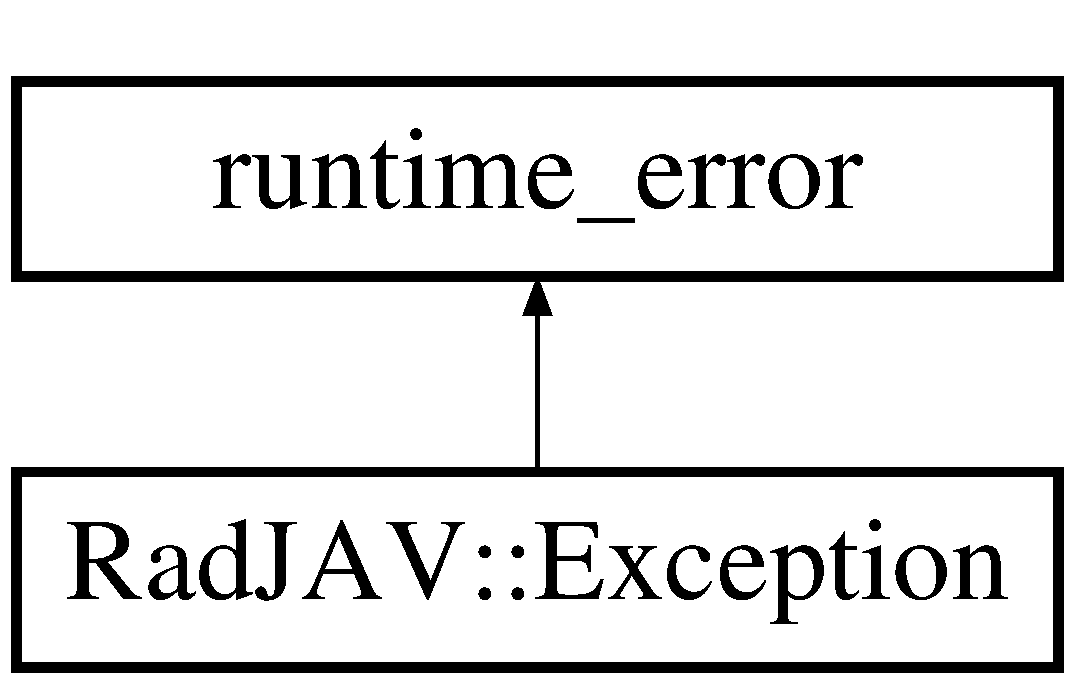
\includegraphics[height=2.000000cm]{class_rad_j_a_v_1_1_exception}
\end{center}
\end{figure}
\subsection*{Public Member Functions}
\begin{DoxyCompactItemize}
\item 
\mbox{\hyperlink{class_rad_j_a_v_1_1_exception_ac29a4a87089f239315155858aa2f9bad}{Exception}} (\mbox{\hyperlink{class_rad_j_a_v_1_1_string}{String}} message)
\item 
\mbox{\hyperlink{class_rad_j_a_v_1_1_string}{String}} \mbox{\hyperlink{class_rad_j_a_v_1_1_exception_ad996ff7a0fcb2b357beff4742cc759ea}{get\+Message}} ()
\end{DoxyCompactItemize}


\subsection{Constructor \& Destructor Documentation}
\mbox{\Hypertarget{class_rad_j_a_v_1_1_exception_ac29a4a87089f239315155858aa2f9bad}\label{class_rad_j_a_v_1_1_exception_ac29a4a87089f239315155858aa2f9bad}} 
\index{Rad\+J\+A\+V\+::\+Exception@{Rad\+J\+A\+V\+::\+Exception}!Exception@{Exception}}
\index{Exception@{Exception}!Rad\+J\+A\+V\+::\+Exception@{Rad\+J\+A\+V\+::\+Exception}}
\subsubsection{\texorpdfstring{Exception()}{Exception()}}
{\footnotesize\ttfamily Rad\+J\+A\+V\+::\+Exception\+::\+Exception (\begin{DoxyParamCaption}\item[{\mbox{\hyperlink{class_rad_j_a_v_1_1_string}{String}}}]{message }\end{DoxyParamCaption})\hspace{0.3cm}{\ttfamily [inline]}}



\subsection{Member Function Documentation}
\mbox{\Hypertarget{class_rad_j_a_v_1_1_exception_ad996ff7a0fcb2b357beff4742cc759ea}\label{class_rad_j_a_v_1_1_exception_ad996ff7a0fcb2b357beff4742cc759ea}} 
\index{Rad\+J\+A\+V\+::\+Exception@{Rad\+J\+A\+V\+::\+Exception}!get\+Message@{get\+Message}}
\index{get\+Message@{get\+Message}!Rad\+J\+A\+V\+::\+Exception@{Rad\+J\+A\+V\+::\+Exception}}
\subsubsection{\texorpdfstring{get\+Message()}{getMessage()}}
{\footnotesize\ttfamily \mbox{\hyperlink{class_rad_j_a_v_1_1_string}{String}} Rad\+J\+A\+V\+::\+Exception\+::get\+Message (\begin{DoxyParamCaption}{ }\end{DoxyParamCaption})\hspace{0.3cm}{\ttfamily [inline]}}



The documentation for this class was generated from the following file\+:\begin{DoxyCompactItemize}
\item 
include/\+Rad\+Jav/\mbox{\hyperlink{_rad_jav_exception_8h}{Rad\+Jav\+Exception.\+h}}\end{DoxyCompactItemize}

\hypertarget{class_rad_j_a_v_1_1_g_u_i_1_1_g_object}{}\section{Rad\+J\+AV\+:\+:G\+UI\+:\+:G\+Object Class Reference}
\label{class_rad_j_a_v_1_1_g_u_i_1_1_g_object}\index{Rad\+J\+A\+V\+::\+G\+U\+I\+::\+G\+Object@{Rad\+J\+A\+V\+::\+G\+U\+I\+::\+G\+Object}}


{\ttfamily \#include $<$Rad\+Jav\+G\+U\+I\+G\+Object.\+h$>$}

Inheritance diagram for Rad\+J\+AV\+:\+:G\+UI\+:\+:G\+Object\+:\begin{figure}[H]
\begin{center}
\leavevmode
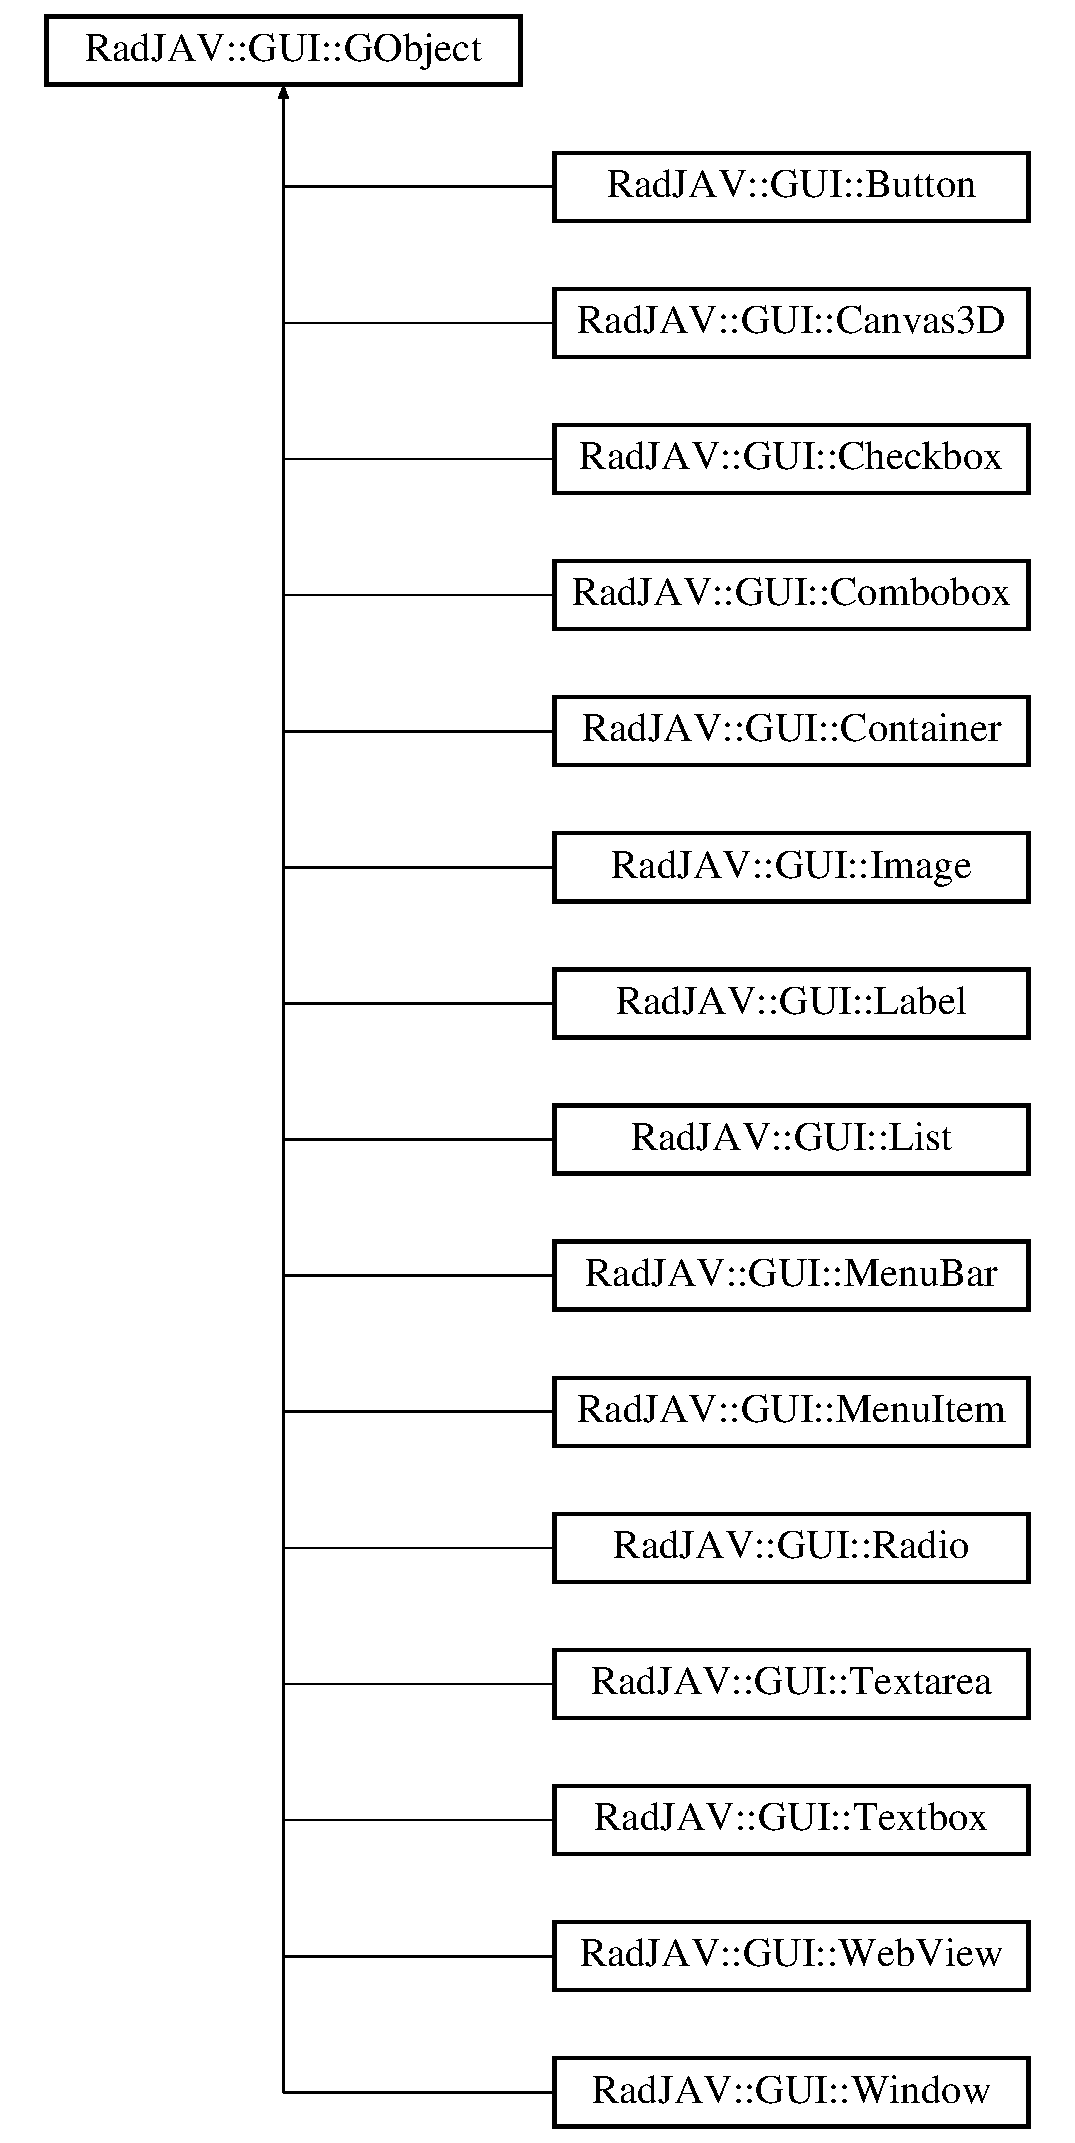
\includegraphics[height=2.000000cm]{class_rad_j_a_v_1_1_g_u_i_1_1_g_object}
\end{center}
\end{figure}
\subsection*{Public Member Functions}
\begin{DoxyCompactItemize}
\item 
\hyperlink{class_rad_j_a_v_1_1_g_u_i_1_1_g_object_a55ca56da5ee42b7b8dffdbf22024323f}{G\+Object} (\hyperlink{class_rad_j_a_v_1_1_string}{String} new\+Name)
\item 
\hyperlink{class_rad_j_a_v_1_1_g_u_i_1_1_g_object_a1aacac49c284797fab74ece1298fc3a5}{G\+Object} (\hyperlink{class_rad_j_a_v_1_1_string}{String} new\+Name, \hyperlink{class_rad_j_a_v_1_1_string}{String} new\+Text)
\item 
\hyperlink{class_rad_j_a_v_1_1_g_u_i_1_1_g_object_a354230117eeeda4b2fde9c114833dba6}{G\+Object} (\hyperlink{class_rad_j_a_v_1_1_string}{String} new\+Name, \hyperlink{class_rad_j_a_v_1_1_string}{String} new\+Text, std\+::shared\+\_\+ptr$<$ \hyperlink{class_rad_j_a_v_1_1_g_u_i_1_1_g_object}{G\+Object} $>$ new\+Parent)
\item 
virtual void \hyperlink{class_rad_j_a_v_1_1_g_u_i_1_1_g_object_a0758b7d4b69fc985c20c8dc680c8464c}{create} ()=0
\begin{DoxyCompactList}\small\item\em Create the object. \end{DoxyCompactList}\item 
virtual void \hyperlink{class_rad_j_a_v_1_1_g_u_i_1_1_g_object_a4fa92764a95242183fcb3758483d5d7d}{set\+Position} (R\+D\+E\+C\+I\+M\+AL x, R\+D\+E\+C\+I\+M\+AL y)
\begin{DoxyCompactList}\small\item\em Set the position of this object. \end{DoxyCompactList}\item 
virtual \hyperlink{class_rad_j_a_v_1_1_vector2}{Vector2} \hyperlink{class_rad_j_a_v_1_1_g_u_i_1_1_g_object_adc0cac980eb118e93aa39b5cd72c9602}{get\+Position} ()
\begin{DoxyCompactList}\small\item\em Get the position of this object. \end{DoxyCompactList}\item 
virtual void \hyperlink{class_rad_j_a_v_1_1_g_u_i_1_1_g_object_a2249e2abbb4cafb519512ec9c95f9d5e}{set\+Size} (R\+D\+E\+C\+I\+M\+AL width, R\+D\+E\+C\+I\+M\+AL height)
\begin{DoxyCompactList}\small\item\em Set the size of this object. \end{DoxyCompactList}\item 
virtual \hyperlink{class_rad_j_a_v_1_1_vector2}{Vector2} \hyperlink{class_rad_j_a_v_1_1_g_u_i_1_1_g_object_a330659366f5b734fc7d84a8a60ec24e5}{get\+Size} ()
\begin{DoxyCompactList}\small\item\em Get the size of this object. \end{DoxyCompactList}\item 
virtual R\+D\+E\+C\+I\+M\+AL \hyperlink{class_rad_j_a_v_1_1_g_u_i_1_1_g_object_a8143f4664e12b03dfe939cd9bf23d5eb}{get\+Width} ()
\begin{DoxyCompactList}\small\item\em Get the width of this object. \end{DoxyCompactList}\item 
virtual R\+D\+E\+C\+I\+M\+AL \hyperlink{class_rad_j_a_v_1_1_g_u_i_1_1_g_object_a333cb3617fcc8d3446c67ea12690d63f}{get\+Height} ()
\begin{DoxyCompactList}\small\item\em Get the height of this object. \end{DoxyCompactList}\item 
virtual void \hyperlink{class_rad_j_a_v_1_1_g_u_i_1_1_g_object_a361fe7962341e8d0562b39d28ad1b465}{set\+Text} (\hyperlink{class_rad_j_a_v_1_1_string}{String} new\+Text)=0
\begin{DoxyCompactList}\small\item\em Set the object\textquotesingle{}s text. \end{DoxyCompactList}\item 
virtual \hyperlink{class_rad_j_a_v_1_1_string}{String} \hyperlink{class_rad_j_a_v_1_1_g_u_i_1_1_g_object_a623610eb55210a2f88afbdeda31f088e}{get\+Text} ()=0
\begin{DoxyCompactList}\small\item\em Get the object\textquotesingle{}s text. \end{DoxyCompactList}\item 
virtual std\+::shared\+\_\+ptr$<$ \hyperlink{class_rad_j_a_v_1_1_g_u_i_1_1_g_object}{G\+Object} $>$ \hyperlink{class_rad_j_a_v_1_1_g_u_i_1_1_g_object_a81dfe857a4bd89de9214982d30a28ce5}{get\+Parent} ()
\begin{DoxyCompactList}\small\item\em Get the parent. \end{DoxyCompactList}\item 
virtual std\+::shared\+\_\+ptr$<$ \hyperlink{class_rad_j_a_v_1_1_g_u_i_1_1_g_object}{G\+Object} $>$ \hyperlink{class_rad_j_a_v_1_1_g_u_i_1_1_g_object_abdd66443a236cf9b0d6f76d826ce4565}{get\+G\+U\+I\+Object} ()
\begin{DoxyCompactList}\small\item\em Get OS level \hyperlink{namespace_rad_j_a_v_1_1_g_u_i}{G\+UI} object associated with this object. \end{DoxyCompactList}\item 
virtual void \hyperlink{class_rad_j_a_v_1_1_g_u_i_1_1_g_object_a108ec023dce72af50ce3bbe5fb61b394}{set\+Visibility} (bool new\+Visible)=0
\begin{DoxyCompactList}\small\item\em Set the visibility of this object. \end{DoxyCompactList}\item 
virtual bool \hyperlink{class_rad_j_a_v_1_1_g_u_i_1_1_g_object_a9b30394c246dc1cce788c93e48e6e00d}{get\+Visibility} ()=0
\begin{DoxyCompactList}\small\item\em Get the visibility of this object. \end{DoxyCompactList}\item 
virtual void \hyperlink{class_rad_j_a_v_1_1_g_u_i_1_1_g_object_acaa57b7783df4cdc6a2e2bab0eb783a9}{show} ()
\begin{DoxyCompactList}\small\item\em Show this object. \end{DoxyCompactList}\item 
virtual void \hyperlink{class_rad_j_a_v_1_1_g_u_i_1_1_g_object_a7b05cad20d34e3eb5fc411dbb4834f9a}{hide} ()
\begin{DoxyCompactList}\small\item\em Hide this object. \end{DoxyCompactList}\item 
virtual void \hyperlink{class_rad_j_a_v_1_1_g_u_i_1_1_g_object_a224cec9275e8e5197d813ac5996f713c}{on} (\hyperlink{class_rad_j_a_v_1_1_string}{String} event\+Name, std\+::function$<$ void()$>$ func)=0
\begin{DoxyCompactList}\small\item\em Calls a function when an event is triggered. \end{DoxyCompactList}\end{DoxyCompactItemize}
\subsection*{Protected Member Functions}
\begin{DoxyCompactItemize}
\item 
void \hyperlink{class_rad_j_a_v_1_1_g_u_i_1_1_g_object_ad4d38f180cae50247bd585ba4cf5e7ac}{finished\+Creating} (std\+::shared\+\_\+ptr$<$ void $>$ new\+Gui\+Object)
\begin{DoxyCompactList}\small\item\em Call when the object has finished creating. \end{DoxyCompactList}\end{DoxyCompactItemize}
\subsection*{Protected Attributes}
\begin{DoxyCompactItemize}
\item 
\hyperlink{class_rad_j_a_v_1_1_string}{String} \hyperlink{class_rad_j_a_v_1_1_g_u_i_1_1_g_object_ab9558e5a1d782f881930b297b2ee4ccc}{name}
\begin{DoxyCompactList}\small\item\em The name of this object. \end{DoxyCompactList}\item 
\hyperlink{class_rad_j_a_v_1_1_string}{String} \hyperlink{class_rad_j_a_v_1_1_g_u_i_1_1_g_object_a11b7855ac57a7bfc041b87f0cdd0abd3}{type}
\begin{DoxyCompactList}\small\item\em The type of object. \end{DoxyCompactList}\item 
std\+::shared\+\_\+ptr$<$ \hyperlink{class_rad_j_a_v_1_1_rectangle}{Rectangle} $>$ \hyperlink{class_rad_j_a_v_1_1_g_u_i_1_1_g_object_abfe4fed9fc8c89417082f6c39575b5a3}{transform}
\begin{DoxyCompactList}\small\item\em The transform of this object. \end{DoxyCompactList}\item 
bool \hyperlink{class_rad_j_a_v_1_1_g_u_i_1_1_g_object_a5c9f1e09ab9ed387d0b069e940beed72}{visible}
\begin{DoxyCompactList}\small\item\em The visibility of the object. \end{DoxyCompactList}\item 
\hyperlink{class_rad_j_a_v_1_1_string}{String} \hyperlink{class_rad_j_a_v_1_1_g_u_i_1_1_g_object_a1793a275a95be0b663a00be60f0b6db2}{text}
\begin{DoxyCompactList}\small\item\em The text associated with this object. \end{DoxyCompactList}\item 
std\+::shared\+\_\+ptr$<$ \hyperlink{class_rad_j_a_v_1_1_g_u_i_1_1_g_object}{G\+Object} $>$ \hyperlink{class_rad_j_a_v_1_1_g_u_i_1_1_g_object_aabe842f535f5eb754c7aac935d3dff0d}{parent}
\begin{DoxyCompactList}\small\item\em The parent of this object. \end{DoxyCompactList}\item 
std\+::shared\+\_\+ptr$<$ void $>$ \hyperlink{class_rad_j_a_v_1_1_g_u_i_1_1_g_object_acba108b6a5e5b4560b493c291cdbb7a3}{gui\+Object}
\begin{DoxyCompactList}\small\item\em The OS level \hyperlink{namespace_rad_j_a_v_1_1_g_u_i}{G\+UI} Object associated with this object. \end{DoxyCompactList}\end{DoxyCompactItemize}


\subsection{Constructor \& Destructor Documentation}
\index{Rad\+J\+A\+V\+::\+G\+U\+I\+::\+G\+Object@{Rad\+J\+A\+V\+::\+G\+U\+I\+::\+G\+Object}!G\+Object@{G\+Object}}
\index{G\+Object@{G\+Object}!Rad\+J\+A\+V\+::\+G\+U\+I\+::\+G\+Object@{Rad\+J\+A\+V\+::\+G\+U\+I\+::\+G\+Object}}
\subsubsection[{\texorpdfstring{G\+Object(\+String new\+Name)}{GObject(String newName)}}]{\setlength{\rightskip}{0pt plus 5cm}Rad\+J\+A\+V\+::\+G\+U\+I\+::\+G\+Object\+::\+G\+Object (
\begin{DoxyParamCaption}
\item[{{\bf String}}]{new\+Name}
\end{DoxyParamCaption}
)}\hypertarget{class_rad_j_a_v_1_1_g_u_i_1_1_g_object_a55ca56da5ee42b7b8dffdbf22024323f}{}\label{class_rad_j_a_v_1_1_g_u_i_1_1_g_object_a55ca56da5ee42b7b8dffdbf22024323f}
\index{Rad\+J\+A\+V\+::\+G\+U\+I\+::\+G\+Object@{Rad\+J\+A\+V\+::\+G\+U\+I\+::\+G\+Object}!G\+Object@{G\+Object}}
\index{G\+Object@{G\+Object}!Rad\+J\+A\+V\+::\+G\+U\+I\+::\+G\+Object@{Rad\+J\+A\+V\+::\+G\+U\+I\+::\+G\+Object}}
\subsubsection[{\texorpdfstring{G\+Object(\+String new\+Name, String new\+Text)}{GObject(String newName, String newText)}}]{\setlength{\rightskip}{0pt plus 5cm}Rad\+J\+A\+V\+::\+G\+U\+I\+::\+G\+Object\+::\+G\+Object (
\begin{DoxyParamCaption}
\item[{{\bf String}}]{new\+Name, }
\item[{{\bf String}}]{new\+Text}
\end{DoxyParamCaption}
)}\hypertarget{class_rad_j_a_v_1_1_g_u_i_1_1_g_object_a1aacac49c284797fab74ece1298fc3a5}{}\label{class_rad_j_a_v_1_1_g_u_i_1_1_g_object_a1aacac49c284797fab74ece1298fc3a5}
\index{Rad\+J\+A\+V\+::\+G\+U\+I\+::\+G\+Object@{Rad\+J\+A\+V\+::\+G\+U\+I\+::\+G\+Object}!G\+Object@{G\+Object}}
\index{G\+Object@{G\+Object}!Rad\+J\+A\+V\+::\+G\+U\+I\+::\+G\+Object@{Rad\+J\+A\+V\+::\+G\+U\+I\+::\+G\+Object}}
\subsubsection[{\texorpdfstring{G\+Object(\+String new\+Name, String new\+Text, std\+::shared\+\_\+ptr$<$ G\+Object $>$ new\+Parent)}{GObject(String newName, String newText, std::shared_ptr< GObject > newParent)}}]{\setlength{\rightskip}{0pt plus 5cm}Rad\+J\+A\+V\+::\+G\+U\+I\+::\+G\+Object\+::\+G\+Object (
\begin{DoxyParamCaption}
\item[{{\bf String}}]{new\+Name, }
\item[{{\bf String}}]{new\+Text, }
\item[{std\+::shared\+\_\+ptr$<$ {\bf G\+Object} $>$}]{new\+Parent}
\end{DoxyParamCaption}
)}\hypertarget{class_rad_j_a_v_1_1_g_u_i_1_1_g_object_a354230117eeeda4b2fde9c114833dba6}{}\label{class_rad_j_a_v_1_1_g_u_i_1_1_g_object_a354230117eeeda4b2fde9c114833dba6}


\subsection{Member Function Documentation}
\index{Rad\+J\+A\+V\+::\+G\+U\+I\+::\+G\+Object@{Rad\+J\+A\+V\+::\+G\+U\+I\+::\+G\+Object}!create@{create}}
\index{create@{create}!Rad\+J\+A\+V\+::\+G\+U\+I\+::\+G\+Object@{Rad\+J\+A\+V\+::\+G\+U\+I\+::\+G\+Object}}
\subsubsection[{\texorpdfstring{create()=0}{create()=0}}]{\setlength{\rightskip}{0pt plus 5cm}virtual void Rad\+J\+A\+V\+::\+G\+U\+I\+::\+G\+Object\+::create (
\begin{DoxyParamCaption}
{}
\end{DoxyParamCaption}
)\hspace{0.3cm}{\ttfamily [pure virtual]}}\hypertarget{class_rad_j_a_v_1_1_g_u_i_1_1_g_object_a0758b7d4b69fc985c20c8dc680c8464c}{}\label{class_rad_j_a_v_1_1_g_u_i_1_1_g_object_a0758b7d4b69fc985c20c8dc680c8464c}


Create the object. 



Implemented in \hyperlink{class_rad_j_a_v_1_1_g_u_i_1_1_window_a92bf59c30dd5b9f77d77a31f9a2f8982}{Rad\+J\+A\+V\+::\+G\+U\+I\+::\+Window}.

\index{Rad\+J\+A\+V\+::\+G\+U\+I\+::\+G\+Object@{Rad\+J\+A\+V\+::\+G\+U\+I\+::\+G\+Object}!finished\+Creating@{finished\+Creating}}
\index{finished\+Creating@{finished\+Creating}!Rad\+J\+A\+V\+::\+G\+U\+I\+::\+G\+Object@{Rad\+J\+A\+V\+::\+G\+U\+I\+::\+G\+Object}}
\subsubsection[{\texorpdfstring{finished\+Creating(std\+::shared\+\_\+ptr$<$ void $>$ new\+Gui\+Object)}{finishedCreating(std::shared_ptr< void > newGuiObject)}}]{\setlength{\rightskip}{0pt plus 5cm}void Rad\+J\+A\+V\+::\+G\+U\+I\+::\+G\+Object\+::finished\+Creating (
\begin{DoxyParamCaption}
\item[{std\+::shared\+\_\+ptr$<$ void $>$}]{new\+Gui\+Object}
\end{DoxyParamCaption}
)\hspace{0.3cm}{\ttfamily [inline]}, {\ttfamily [protected]}}\hypertarget{class_rad_j_a_v_1_1_g_u_i_1_1_g_object_ad4d38f180cae50247bd585ba4cf5e7ac}{}\label{class_rad_j_a_v_1_1_g_u_i_1_1_g_object_ad4d38f180cae50247bd585ba4cf5e7ac}


Call when the object has finished creating. 

\index{Rad\+J\+A\+V\+::\+G\+U\+I\+::\+G\+Object@{Rad\+J\+A\+V\+::\+G\+U\+I\+::\+G\+Object}!get\+G\+U\+I\+Object@{get\+G\+U\+I\+Object}}
\index{get\+G\+U\+I\+Object@{get\+G\+U\+I\+Object}!Rad\+J\+A\+V\+::\+G\+U\+I\+::\+G\+Object@{Rad\+J\+A\+V\+::\+G\+U\+I\+::\+G\+Object}}
\subsubsection[{\texorpdfstring{get\+G\+U\+I\+Object()}{getGUIObject()}}]{\setlength{\rightskip}{0pt plus 5cm}virtual std\+::shared\+\_\+ptr$<${\bf G\+Object}$>$ Rad\+J\+A\+V\+::\+G\+U\+I\+::\+G\+Object\+::get\+G\+U\+I\+Object (
\begin{DoxyParamCaption}
{}
\end{DoxyParamCaption}
)\hspace{0.3cm}{\ttfamily [inline]}, {\ttfamily [virtual]}}\hypertarget{class_rad_j_a_v_1_1_g_u_i_1_1_g_object_abdd66443a236cf9b0d6f76d826ce4565}{}\label{class_rad_j_a_v_1_1_g_u_i_1_1_g_object_abdd66443a236cf9b0d6f76d826ce4565}


Get OS level \hyperlink{namespace_rad_j_a_v_1_1_g_u_i}{G\+UI} object associated with this object. 

\index{Rad\+J\+A\+V\+::\+G\+U\+I\+::\+G\+Object@{Rad\+J\+A\+V\+::\+G\+U\+I\+::\+G\+Object}!get\+Height@{get\+Height}}
\index{get\+Height@{get\+Height}!Rad\+J\+A\+V\+::\+G\+U\+I\+::\+G\+Object@{Rad\+J\+A\+V\+::\+G\+U\+I\+::\+G\+Object}}
\subsubsection[{\texorpdfstring{get\+Height()}{getHeight()}}]{\setlength{\rightskip}{0pt plus 5cm}virtual R\+D\+E\+C\+I\+M\+AL Rad\+J\+A\+V\+::\+G\+U\+I\+::\+G\+Object\+::get\+Height (
\begin{DoxyParamCaption}
{}
\end{DoxyParamCaption}
)\hspace{0.3cm}{\ttfamily [inline]}, {\ttfamily [virtual]}}\hypertarget{class_rad_j_a_v_1_1_g_u_i_1_1_g_object_a333cb3617fcc8d3446c67ea12690d63f}{}\label{class_rad_j_a_v_1_1_g_u_i_1_1_g_object_a333cb3617fcc8d3446c67ea12690d63f}


Get the height of this object. 

\index{Rad\+J\+A\+V\+::\+G\+U\+I\+::\+G\+Object@{Rad\+J\+A\+V\+::\+G\+U\+I\+::\+G\+Object}!get\+Parent@{get\+Parent}}
\index{get\+Parent@{get\+Parent}!Rad\+J\+A\+V\+::\+G\+U\+I\+::\+G\+Object@{Rad\+J\+A\+V\+::\+G\+U\+I\+::\+G\+Object}}
\subsubsection[{\texorpdfstring{get\+Parent()}{getParent()}}]{\setlength{\rightskip}{0pt plus 5cm}virtual std\+::shared\+\_\+ptr$<${\bf G\+Object}$>$ Rad\+J\+A\+V\+::\+G\+U\+I\+::\+G\+Object\+::get\+Parent (
\begin{DoxyParamCaption}
{}
\end{DoxyParamCaption}
)\hspace{0.3cm}{\ttfamily [inline]}, {\ttfamily [virtual]}}\hypertarget{class_rad_j_a_v_1_1_g_u_i_1_1_g_object_a81dfe857a4bd89de9214982d30a28ce5}{}\label{class_rad_j_a_v_1_1_g_u_i_1_1_g_object_a81dfe857a4bd89de9214982d30a28ce5}


Get the parent. 

\index{Rad\+J\+A\+V\+::\+G\+U\+I\+::\+G\+Object@{Rad\+J\+A\+V\+::\+G\+U\+I\+::\+G\+Object}!get\+Position@{get\+Position}}
\index{get\+Position@{get\+Position}!Rad\+J\+A\+V\+::\+G\+U\+I\+::\+G\+Object@{Rad\+J\+A\+V\+::\+G\+U\+I\+::\+G\+Object}}
\subsubsection[{\texorpdfstring{get\+Position()}{getPosition()}}]{\setlength{\rightskip}{0pt plus 5cm}{\bf Vector2} Rad\+J\+A\+V\+::\+G\+U\+I\+::\+G\+Object\+::get\+Position (
\begin{DoxyParamCaption}
{}
\end{DoxyParamCaption}
)\hspace{0.3cm}{\ttfamily [virtual]}}\hypertarget{class_rad_j_a_v_1_1_g_u_i_1_1_g_object_adc0cac980eb118e93aa39b5cd72c9602}{}\label{class_rad_j_a_v_1_1_g_u_i_1_1_g_object_adc0cac980eb118e93aa39b5cd72c9602}


Get the position of this object. 

\index{Rad\+J\+A\+V\+::\+G\+U\+I\+::\+G\+Object@{Rad\+J\+A\+V\+::\+G\+U\+I\+::\+G\+Object}!get\+Size@{get\+Size}}
\index{get\+Size@{get\+Size}!Rad\+J\+A\+V\+::\+G\+U\+I\+::\+G\+Object@{Rad\+J\+A\+V\+::\+G\+U\+I\+::\+G\+Object}}
\subsubsection[{\texorpdfstring{get\+Size()}{getSize()}}]{\setlength{\rightskip}{0pt plus 5cm}{\bf Vector2} Rad\+J\+A\+V\+::\+G\+U\+I\+::\+G\+Object\+::get\+Size (
\begin{DoxyParamCaption}
{}
\end{DoxyParamCaption}
)\hspace{0.3cm}{\ttfamily [virtual]}}\hypertarget{class_rad_j_a_v_1_1_g_u_i_1_1_g_object_a330659366f5b734fc7d84a8a60ec24e5}{}\label{class_rad_j_a_v_1_1_g_u_i_1_1_g_object_a330659366f5b734fc7d84a8a60ec24e5}


Get the size of this object. 

\index{Rad\+J\+A\+V\+::\+G\+U\+I\+::\+G\+Object@{Rad\+J\+A\+V\+::\+G\+U\+I\+::\+G\+Object}!get\+Text@{get\+Text}}
\index{get\+Text@{get\+Text}!Rad\+J\+A\+V\+::\+G\+U\+I\+::\+G\+Object@{Rad\+J\+A\+V\+::\+G\+U\+I\+::\+G\+Object}}
\subsubsection[{\texorpdfstring{get\+Text()=0}{getText()=0}}]{\setlength{\rightskip}{0pt plus 5cm}virtual {\bf String} Rad\+J\+A\+V\+::\+G\+U\+I\+::\+G\+Object\+::get\+Text (
\begin{DoxyParamCaption}
{}
\end{DoxyParamCaption}
)\hspace{0.3cm}{\ttfamily [pure virtual]}}\hypertarget{class_rad_j_a_v_1_1_g_u_i_1_1_g_object_a623610eb55210a2f88afbdeda31f088e}{}\label{class_rad_j_a_v_1_1_g_u_i_1_1_g_object_a623610eb55210a2f88afbdeda31f088e}


Get the object\textquotesingle{}s text. 



Implemented in \hyperlink{class_rad_j_a_v_1_1_g_u_i_1_1_window_a91a0cb7a172dc0ff1e378706b033cf3d}{Rad\+J\+A\+V\+::\+G\+U\+I\+::\+Window}.

\index{Rad\+J\+A\+V\+::\+G\+U\+I\+::\+G\+Object@{Rad\+J\+A\+V\+::\+G\+U\+I\+::\+G\+Object}!get\+Visibility@{get\+Visibility}}
\index{get\+Visibility@{get\+Visibility}!Rad\+J\+A\+V\+::\+G\+U\+I\+::\+G\+Object@{Rad\+J\+A\+V\+::\+G\+U\+I\+::\+G\+Object}}
\subsubsection[{\texorpdfstring{get\+Visibility()=0}{getVisibility()=0}}]{\setlength{\rightskip}{0pt plus 5cm}virtual bool Rad\+J\+A\+V\+::\+G\+U\+I\+::\+G\+Object\+::get\+Visibility (
\begin{DoxyParamCaption}
{}
\end{DoxyParamCaption}
)\hspace{0.3cm}{\ttfamily [pure virtual]}}\hypertarget{class_rad_j_a_v_1_1_g_u_i_1_1_g_object_a9b30394c246dc1cce788c93e48e6e00d}{}\label{class_rad_j_a_v_1_1_g_u_i_1_1_g_object_a9b30394c246dc1cce788c93e48e6e00d}


Get the visibility of this object. 



Implemented in \hyperlink{class_rad_j_a_v_1_1_g_u_i_1_1_window_a4ddb8d5a94c7fcaadb1bed004c80561b}{Rad\+J\+A\+V\+::\+G\+U\+I\+::\+Window}.

\index{Rad\+J\+A\+V\+::\+G\+U\+I\+::\+G\+Object@{Rad\+J\+A\+V\+::\+G\+U\+I\+::\+G\+Object}!get\+Width@{get\+Width}}
\index{get\+Width@{get\+Width}!Rad\+J\+A\+V\+::\+G\+U\+I\+::\+G\+Object@{Rad\+J\+A\+V\+::\+G\+U\+I\+::\+G\+Object}}
\subsubsection[{\texorpdfstring{get\+Width()}{getWidth()}}]{\setlength{\rightskip}{0pt plus 5cm}virtual R\+D\+E\+C\+I\+M\+AL Rad\+J\+A\+V\+::\+G\+U\+I\+::\+G\+Object\+::get\+Width (
\begin{DoxyParamCaption}
{}
\end{DoxyParamCaption}
)\hspace{0.3cm}{\ttfamily [inline]}, {\ttfamily [virtual]}}\hypertarget{class_rad_j_a_v_1_1_g_u_i_1_1_g_object_a8143f4664e12b03dfe939cd9bf23d5eb}{}\label{class_rad_j_a_v_1_1_g_u_i_1_1_g_object_a8143f4664e12b03dfe939cd9bf23d5eb}


Get the width of this object. 

\index{Rad\+J\+A\+V\+::\+G\+U\+I\+::\+G\+Object@{Rad\+J\+A\+V\+::\+G\+U\+I\+::\+G\+Object}!hide@{hide}}
\index{hide@{hide}!Rad\+J\+A\+V\+::\+G\+U\+I\+::\+G\+Object@{Rad\+J\+A\+V\+::\+G\+U\+I\+::\+G\+Object}}
\subsubsection[{\texorpdfstring{hide()}{hide()}}]{\setlength{\rightskip}{0pt plus 5cm}virtual void Rad\+J\+A\+V\+::\+G\+U\+I\+::\+G\+Object\+::hide (
\begin{DoxyParamCaption}
{}
\end{DoxyParamCaption}
)\hspace{0.3cm}{\ttfamily [inline]}, {\ttfamily [virtual]}}\hypertarget{class_rad_j_a_v_1_1_g_u_i_1_1_g_object_a7b05cad20d34e3eb5fc411dbb4834f9a}{}\label{class_rad_j_a_v_1_1_g_u_i_1_1_g_object_a7b05cad20d34e3eb5fc411dbb4834f9a}


Hide this object. 

\index{Rad\+J\+A\+V\+::\+G\+U\+I\+::\+G\+Object@{Rad\+J\+A\+V\+::\+G\+U\+I\+::\+G\+Object}!on@{on}}
\index{on@{on}!Rad\+J\+A\+V\+::\+G\+U\+I\+::\+G\+Object@{Rad\+J\+A\+V\+::\+G\+U\+I\+::\+G\+Object}}
\subsubsection[{\texorpdfstring{on(\+String event\+Name, std\+::function$<$ void()$>$ func)=0}{on(String eventName, std::function< void()> func)=0}}]{\setlength{\rightskip}{0pt plus 5cm}virtual void Rad\+J\+A\+V\+::\+G\+U\+I\+::\+G\+Object\+::on (
\begin{DoxyParamCaption}
\item[{{\bf String}}]{event\+Name, }
\item[{std\+::function$<$ void()$>$}]{func}
\end{DoxyParamCaption}
)\hspace{0.3cm}{\ttfamily [pure virtual]}}\hypertarget{class_rad_j_a_v_1_1_g_u_i_1_1_g_object_a224cec9275e8e5197d813ac5996f713c}{}\label{class_rad_j_a_v_1_1_g_u_i_1_1_g_object_a224cec9275e8e5197d813ac5996f713c}


Calls a function when an event is triggered. 



Implemented in \hyperlink{class_rad_j_a_v_1_1_g_u_i_1_1_window_a0b9e73f35922418bd2a6c52d349b8bcf}{Rad\+J\+A\+V\+::\+G\+U\+I\+::\+Window}.

\index{Rad\+J\+A\+V\+::\+G\+U\+I\+::\+G\+Object@{Rad\+J\+A\+V\+::\+G\+U\+I\+::\+G\+Object}!set\+Position@{set\+Position}}
\index{set\+Position@{set\+Position}!Rad\+J\+A\+V\+::\+G\+U\+I\+::\+G\+Object@{Rad\+J\+A\+V\+::\+G\+U\+I\+::\+G\+Object}}
\subsubsection[{\texorpdfstring{set\+Position(\+R\+D\+E\+C\+I\+M\+A\+L x, R\+D\+E\+C\+I\+M\+A\+L y)}{setPosition(RDECIMAL x, RDECIMAL y)}}]{\setlength{\rightskip}{0pt plus 5cm}void Rad\+J\+A\+V\+::\+G\+U\+I\+::\+G\+Object\+::set\+Position (
\begin{DoxyParamCaption}
\item[{R\+D\+E\+C\+I\+M\+AL}]{x, }
\item[{R\+D\+E\+C\+I\+M\+AL}]{y}
\end{DoxyParamCaption}
)\hspace{0.3cm}{\ttfamily [virtual]}}\hypertarget{class_rad_j_a_v_1_1_g_u_i_1_1_g_object_a4fa92764a95242183fcb3758483d5d7d}{}\label{class_rad_j_a_v_1_1_g_u_i_1_1_g_object_a4fa92764a95242183fcb3758483d5d7d}


Set the position of this object. 

\index{Rad\+J\+A\+V\+::\+G\+U\+I\+::\+G\+Object@{Rad\+J\+A\+V\+::\+G\+U\+I\+::\+G\+Object}!set\+Size@{set\+Size}}
\index{set\+Size@{set\+Size}!Rad\+J\+A\+V\+::\+G\+U\+I\+::\+G\+Object@{Rad\+J\+A\+V\+::\+G\+U\+I\+::\+G\+Object}}
\subsubsection[{\texorpdfstring{set\+Size(\+R\+D\+E\+C\+I\+M\+A\+L width, R\+D\+E\+C\+I\+M\+A\+L height)}{setSize(RDECIMAL width, RDECIMAL height)}}]{\setlength{\rightskip}{0pt plus 5cm}void Rad\+J\+A\+V\+::\+G\+U\+I\+::\+G\+Object\+::set\+Size (
\begin{DoxyParamCaption}
\item[{R\+D\+E\+C\+I\+M\+AL}]{width, }
\item[{R\+D\+E\+C\+I\+M\+AL}]{height}
\end{DoxyParamCaption}
)\hspace{0.3cm}{\ttfamily [virtual]}}\hypertarget{class_rad_j_a_v_1_1_g_u_i_1_1_g_object_a2249e2abbb4cafb519512ec9c95f9d5e}{}\label{class_rad_j_a_v_1_1_g_u_i_1_1_g_object_a2249e2abbb4cafb519512ec9c95f9d5e}


Set the size of this object. 

\index{Rad\+J\+A\+V\+::\+G\+U\+I\+::\+G\+Object@{Rad\+J\+A\+V\+::\+G\+U\+I\+::\+G\+Object}!set\+Text@{set\+Text}}
\index{set\+Text@{set\+Text}!Rad\+J\+A\+V\+::\+G\+U\+I\+::\+G\+Object@{Rad\+J\+A\+V\+::\+G\+U\+I\+::\+G\+Object}}
\subsubsection[{\texorpdfstring{set\+Text(\+String new\+Text)=0}{setText(String newText)=0}}]{\setlength{\rightskip}{0pt plus 5cm}virtual void Rad\+J\+A\+V\+::\+G\+U\+I\+::\+G\+Object\+::set\+Text (
\begin{DoxyParamCaption}
\item[{{\bf String}}]{new\+Text}
\end{DoxyParamCaption}
)\hspace{0.3cm}{\ttfamily [pure virtual]}}\hypertarget{class_rad_j_a_v_1_1_g_u_i_1_1_g_object_a361fe7962341e8d0562b39d28ad1b465}{}\label{class_rad_j_a_v_1_1_g_u_i_1_1_g_object_a361fe7962341e8d0562b39d28ad1b465}


Set the object\textquotesingle{}s text. 



Implemented in \hyperlink{class_rad_j_a_v_1_1_g_u_i_1_1_window_acbc9c4caf87c4922bafa4b89dc2a9c03}{Rad\+J\+A\+V\+::\+G\+U\+I\+::\+Window}.

\index{Rad\+J\+A\+V\+::\+G\+U\+I\+::\+G\+Object@{Rad\+J\+A\+V\+::\+G\+U\+I\+::\+G\+Object}!set\+Visibility@{set\+Visibility}}
\index{set\+Visibility@{set\+Visibility}!Rad\+J\+A\+V\+::\+G\+U\+I\+::\+G\+Object@{Rad\+J\+A\+V\+::\+G\+U\+I\+::\+G\+Object}}
\subsubsection[{\texorpdfstring{set\+Visibility(bool new\+Visible)=0}{setVisibility(bool newVisible)=0}}]{\setlength{\rightskip}{0pt plus 5cm}virtual void Rad\+J\+A\+V\+::\+G\+U\+I\+::\+G\+Object\+::set\+Visibility (
\begin{DoxyParamCaption}
\item[{bool}]{new\+Visible}
\end{DoxyParamCaption}
)\hspace{0.3cm}{\ttfamily [pure virtual]}}\hypertarget{class_rad_j_a_v_1_1_g_u_i_1_1_g_object_a108ec023dce72af50ce3bbe5fb61b394}{}\label{class_rad_j_a_v_1_1_g_u_i_1_1_g_object_a108ec023dce72af50ce3bbe5fb61b394}


Set the visibility of this object. 



Implemented in \hyperlink{class_rad_j_a_v_1_1_g_u_i_1_1_window_a7e92748e13733aa6c2b15beaaa76ab55}{Rad\+J\+A\+V\+::\+G\+U\+I\+::\+Window}.

\index{Rad\+J\+A\+V\+::\+G\+U\+I\+::\+G\+Object@{Rad\+J\+A\+V\+::\+G\+U\+I\+::\+G\+Object}!show@{show}}
\index{show@{show}!Rad\+J\+A\+V\+::\+G\+U\+I\+::\+G\+Object@{Rad\+J\+A\+V\+::\+G\+U\+I\+::\+G\+Object}}
\subsubsection[{\texorpdfstring{show()}{show()}}]{\setlength{\rightskip}{0pt plus 5cm}virtual void Rad\+J\+A\+V\+::\+G\+U\+I\+::\+G\+Object\+::show (
\begin{DoxyParamCaption}
{}
\end{DoxyParamCaption}
)\hspace{0.3cm}{\ttfamily [inline]}, {\ttfamily [virtual]}}\hypertarget{class_rad_j_a_v_1_1_g_u_i_1_1_g_object_acaa57b7783df4cdc6a2e2bab0eb783a9}{}\label{class_rad_j_a_v_1_1_g_u_i_1_1_g_object_acaa57b7783df4cdc6a2e2bab0eb783a9}


Show this object. 



\subsection{Member Data Documentation}
\index{Rad\+J\+A\+V\+::\+G\+U\+I\+::\+G\+Object@{Rad\+J\+A\+V\+::\+G\+U\+I\+::\+G\+Object}!gui\+Object@{gui\+Object}}
\index{gui\+Object@{gui\+Object}!Rad\+J\+A\+V\+::\+G\+U\+I\+::\+G\+Object@{Rad\+J\+A\+V\+::\+G\+U\+I\+::\+G\+Object}}
\subsubsection[{\texorpdfstring{gui\+Object}{guiObject}}]{\setlength{\rightskip}{0pt plus 5cm}std\+::shared\+\_\+ptr$<$void$>$ Rad\+J\+A\+V\+::\+G\+U\+I\+::\+G\+Object\+::gui\+Object\hspace{0.3cm}{\ttfamily [protected]}}\hypertarget{class_rad_j_a_v_1_1_g_u_i_1_1_g_object_acba108b6a5e5b4560b493c291cdbb7a3}{}\label{class_rad_j_a_v_1_1_g_u_i_1_1_g_object_acba108b6a5e5b4560b493c291cdbb7a3}


The OS level \hyperlink{namespace_rad_j_a_v_1_1_g_u_i}{G\+UI} Object associated with this object. 

\index{Rad\+J\+A\+V\+::\+G\+U\+I\+::\+G\+Object@{Rad\+J\+A\+V\+::\+G\+U\+I\+::\+G\+Object}!name@{name}}
\index{name@{name}!Rad\+J\+A\+V\+::\+G\+U\+I\+::\+G\+Object@{Rad\+J\+A\+V\+::\+G\+U\+I\+::\+G\+Object}}
\subsubsection[{\texorpdfstring{name}{name}}]{\setlength{\rightskip}{0pt plus 5cm}{\bf String} Rad\+J\+A\+V\+::\+G\+U\+I\+::\+G\+Object\+::name\hspace{0.3cm}{\ttfamily [protected]}}\hypertarget{class_rad_j_a_v_1_1_g_u_i_1_1_g_object_ab9558e5a1d782f881930b297b2ee4ccc}{}\label{class_rad_j_a_v_1_1_g_u_i_1_1_g_object_ab9558e5a1d782f881930b297b2ee4ccc}


The name of this object. 

\index{Rad\+J\+A\+V\+::\+G\+U\+I\+::\+G\+Object@{Rad\+J\+A\+V\+::\+G\+U\+I\+::\+G\+Object}!parent@{parent}}
\index{parent@{parent}!Rad\+J\+A\+V\+::\+G\+U\+I\+::\+G\+Object@{Rad\+J\+A\+V\+::\+G\+U\+I\+::\+G\+Object}}
\subsubsection[{\texorpdfstring{parent}{parent}}]{\setlength{\rightskip}{0pt plus 5cm}std\+::shared\+\_\+ptr$<${\bf G\+Object}$>$ Rad\+J\+A\+V\+::\+G\+U\+I\+::\+G\+Object\+::parent\hspace{0.3cm}{\ttfamily [protected]}}\hypertarget{class_rad_j_a_v_1_1_g_u_i_1_1_g_object_aabe842f535f5eb754c7aac935d3dff0d}{}\label{class_rad_j_a_v_1_1_g_u_i_1_1_g_object_aabe842f535f5eb754c7aac935d3dff0d}


The parent of this object. 

\index{Rad\+J\+A\+V\+::\+G\+U\+I\+::\+G\+Object@{Rad\+J\+A\+V\+::\+G\+U\+I\+::\+G\+Object}!text@{text}}
\index{text@{text}!Rad\+J\+A\+V\+::\+G\+U\+I\+::\+G\+Object@{Rad\+J\+A\+V\+::\+G\+U\+I\+::\+G\+Object}}
\subsubsection[{\texorpdfstring{text}{text}}]{\setlength{\rightskip}{0pt plus 5cm}{\bf String} Rad\+J\+A\+V\+::\+G\+U\+I\+::\+G\+Object\+::text\hspace{0.3cm}{\ttfamily [protected]}}\hypertarget{class_rad_j_a_v_1_1_g_u_i_1_1_g_object_a1793a275a95be0b663a00be60f0b6db2}{}\label{class_rad_j_a_v_1_1_g_u_i_1_1_g_object_a1793a275a95be0b663a00be60f0b6db2}


The text associated with this object. 

\index{Rad\+J\+A\+V\+::\+G\+U\+I\+::\+G\+Object@{Rad\+J\+A\+V\+::\+G\+U\+I\+::\+G\+Object}!transform@{transform}}
\index{transform@{transform}!Rad\+J\+A\+V\+::\+G\+U\+I\+::\+G\+Object@{Rad\+J\+A\+V\+::\+G\+U\+I\+::\+G\+Object}}
\subsubsection[{\texorpdfstring{transform}{transform}}]{\setlength{\rightskip}{0pt plus 5cm}std\+::shared\+\_\+ptr$<${\bf Rectangle}$>$ Rad\+J\+A\+V\+::\+G\+U\+I\+::\+G\+Object\+::transform\hspace{0.3cm}{\ttfamily [protected]}}\hypertarget{class_rad_j_a_v_1_1_g_u_i_1_1_g_object_abfe4fed9fc8c89417082f6c39575b5a3}{}\label{class_rad_j_a_v_1_1_g_u_i_1_1_g_object_abfe4fed9fc8c89417082f6c39575b5a3}


The transform of this object. 

\index{Rad\+J\+A\+V\+::\+G\+U\+I\+::\+G\+Object@{Rad\+J\+A\+V\+::\+G\+U\+I\+::\+G\+Object}!type@{type}}
\index{type@{type}!Rad\+J\+A\+V\+::\+G\+U\+I\+::\+G\+Object@{Rad\+J\+A\+V\+::\+G\+U\+I\+::\+G\+Object}}
\subsubsection[{\texorpdfstring{type}{type}}]{\setlength{\rightskip}{0pt plus 5cm}{\bf String} Rad\+J\+A\+V\+::\+G\+U\+I\+::\+G\+Object\+::type\hspace{0.3cm}{\ttfamily [protected]}}\hypertarget{class_rad_j_a_v_1_1_g_u_i_1_1_g_object_a11b7855ac57a7bfc041b87f0cdd0abd3}{}\label{class_rad_j_a_v_1_1_g_u_i_1_1_g_object_a11b7855ac57a7bfc041b87f0cdd0abd3}


The type of object. 

\index{Rad\+J\+A\+V\+::\+G\+U\+I\+::\+G\+Object@{Rad\+J\+A\+V\+::\+G\+U\+I\+::\+G\+Object}!visible@{visible}}
\index{visible@{visible}!Rad\+J\+A\+V\+::\+G\+U\+I\+::\+G\+Object@{Rad\+J\+A\+V\+::\+G\+U\+I\+::\+G\+Object}}
\subsubsection[{\texorpdfstring{visible}{visible}}]{\setlength{\rightskip}{0pt plus 5cm}bool Rad\+J\+A\+V\+::\+G\+U\+I\+::\+G\+Object\+::visible\hspace{0.3cm}{\ttfamily [protected]}}\hypertarget{class_rad_j_a_v_1_1_g_u_i_1_1_g_object_a5c9f1e09ab9ed387d0b069e940beed72}{}\label{class_rad_j_a_v_1_1_g_u_i_1_1_g_object_a5c9f1e09ab9ed387d0b069e940beed72}


The visibility of the object. 



The documentation for this class was generated from the following files\+:\begin{DoxyCompactItemize}
\item 
include/\+Rad\+Jav/\hyperlink{_rad_jav_g_u_i_g_object_8h}{Rad\+Jav\+G\+U\+I\+G\+Object.\+h}\item 
src/\+Rad\+Jav/\hyperlink{_rad_jav_g_u_i_g_object_8cpp}{Rad\+Jav\+G\+U\+I\+G\+Object.\+cpp}\end{DoxyCompactItemize}

\hypertarget{class_rad_j_a_v_1_1_networking_1_1_i_pv4}{}\section{Rad\+J\+AV\+:\+:Networking\+:\+:I\+Pv4 Class Reference}
\label{class_rad_j_a_v_1_1_networking_1_1_i_pv4}\index{Rad\+J\+A\+V\+::\+Networking\+::\+I\+Pv4@{Rad\+J\+A\+V\+::\+Networking\+::\+I\+Pv4}}


{\ttfamily \#include $<$Rad\+Jav\+Networking.\+h$>$}

\subsection*{Public Member Functions}
\begin{DoxyCompactItemize}
\item 
\hyperlink{class_rad_j_a_v_1_1_networking_1_1_i_pv4_a5618bbf3d166d86ded140439fec1b82f}{I\+Pv4} ()
\item 
\hyperlink{class_rad_j_a_v_1_1_networking_1_1_i_pv4_ab139354fc0a0d28ddcae43dc53932ef3}{I\+Pv4} (\hyperlink{class_rad_j_a_v_1_1_string}{String} ip)
\item 
void \hyperlink{class_rad_j_a_v_1_1_networking_1_1_i_pv4_af1ad0c90ed3f6a590bfd7b1de617a699}{get\+I\+Pfrom\+String} (\hyperlink{class_rad_j_a_v_1_1_string}{String} line)
\item 
\hyperlink{class_rad_j_a_v_1_1_string}{String} \hyperlink{class_rad_j_a_v_1_1_networking_1_1_i_pv4_a6c418be8e5836120e69f32e051c1ca8b}{get\+String} ()
\item 
void \hyperlink{class_rad_j_a_v_1_1_networking_1_1_i_pv4_adb180130cd11789b4d2a9e3861e50357}{set} (unsigned short octet1, unsigned short octet2, unsigned short octet3, unsigned short octet4)
\item 
unsigned short $\ast$ \hyperlink{class_rad_j_a_v_1_1_networking_1_1_i_pv4_a685dcb26040092474de0f7b13f27a1ee}{get} ()
\item 
\hyperlink{class_rad_j_a_v_1_1_networking_1_1_i_pv4}{I\+Pv4} \& \hyperlink{class_rad_j_a_v_1_1_networking_1_1_i_pv4_a51d7c276754d08bdc3108eb1270e53ad}{operator=} (\hyperlink{class_rad_j_a_v_1_1_string}{String} ip)
\item 
bool \hyperlink{class_rad_j_a_v_1_1_networking_1_1_i_pv4_a09f3a2a9584caa6295f769a504c58892}{operator==} (\hyperlink{class_rad_j_a_v_1_1_networking_1_1_i_pv4}{I\+Pv4} ip)
\item 
bool \hyperlink{class_rad_j_a_v_1_1_networking_1_1_i_pv4_a7b8886f9baff97314612acda23c4e1ef}{operator==} (\hyperlink{class_rad_j_a_v_1_1_string}{String} ip)
\end{DoxyCompactItemize}
\subsection*{Static Public Member Functions}
\begin{DoxyCompactItemize}
\item 
static \hyperlink{class_rad_j_a_v_1_1_string}{String} \hyperlink{class_rad_j_a_v_1_1_networking_1_1_i_pv4_ae1a87ef33521fe67f22ec3971980eb4e}{get\+String} (\hyperlink{class_rad_j_a_v_1_1_networking_1_1_i_pv4}{I\+Pv4} ippass)
\item 
static \hyperlink{class_rad_j_a_v_1_1_networking_1_1_i_pv4}{I\+Pv4} \hyperlink{class_rad_j_a_v_1_1_networking_1_1_i_pv4_a2d3f283f6256911cbd69404dc204b059}{get\+IP} (\hyperlink{class_rad_j_a_v_1_1_string}{String} line)
\end{DoxyCompactItemize}
\subsection*{Protected Attributes}
\begin{DoxyCompactItemize}
\item 
unsigned short \hyperlink{class_rad_j_a_v_1_1_networking_1_1_i_pv4_afe984ab9f910d7936b42fbb34c428610}{octets} \mbox{[}4\mbox{]}
\end{DoxyCompactItemize}


\subsection{Detailed Description}
Represents an \hyperlink{class_rad_j_a_v_1_1_networking_1_1_i_pv4}{I\+Pv4} address. 

\subsection{Constructor \& Destructor Documentation}
\index{Rad\+J\+A\+V\+::\+Networking\+::\+I\+Pv4@{Rad\+J\+A\+V\+::\+Networking\+::\+I\+Pv4}!I\+Pv4@{I\+Pv4}}
\index{I\+Pv4@{I\+Pv4}!Rad\+J\+A\+V\+::\+Networking\+::\+I\+Pv4@{Rad\+J\+A\+V\+::\+Networking\+::\+I\+Pv4}}
\subsubsection[{\texorpdfstring{I\+Pv4()}{IPv4()}}]{\setlength{\rightskip}{0pt plus 5cm}Rad\+J\+A\+V\+::\+Networking\+::\+I\+Pv4\+::\+I\+Pv4 (
\begin{DoxyParamCaption}
{}
\end{DoxyParamCaption}
)}\hypertarget{class_rad_j_a_v_1_1_networking_1_1_i_pv4_a5618bbf3d166d86ded140439fec1b82f}{}\label{class_rad_j_a_v_1_1_networking_1_1_i_pv4_a5618bbf3d166d86ded140439fec1b82f}
\index{Rad\+J\+A\+V\+::\+Networking\+::\+I\+Pv4@{Rad\+J\+A\+V\+::\+Networking\+::\+I\+Pv4}!I\+Pv4@{I\+Pv4}}
\index{I\+Pv4@{I\+Pv4}!Rad\+J\+A\+V\+::\+Networking\+::\+I\+Pv4@{Rad\+J\+A\+V\+::\+Networking\+::\+I\+Pv4}}
\subsubsection[{\texorpdfstring{I\+Pv4(\+String ip)}{IPv4(String ip)}}]{\setlength{\rightskip}{0pt plus 5cm}Rad\+J\+A\+V\+::\+Networking\+::\+I\+Pv4\+::\+I\+Pv4 (
\begin{DoxyParamCaption}
\item[{{\bf String}}]{ip}
\end{DoxyParamCaption}
)}\hypertarget{class_rad_j_a_v_1_1_networking_1_1_i_pv4_ab139354fc0a0d28ddcae43dc53932ef3}{}\label{class_rad_j_a_v_1_1_networking_1_1_i_pv4_ab139354fc0a0d28ddcae43dc53932ef3}


\subsection{Member Function Documentation}
\index{Rad\+J\+A\+V\+::\+Networking\+::\+I\+Pv4@{Rad\+J\+A\+V\+::\+Networking\+::\+I\+Pv4}!get@{get}}
\index{get@{get}!Rad\+J\+A\+V\+::\+Networking\+::\+I\+Pv4@{Rad\+J\+A\+V\+::\+Networking\+::\+I\+Pv4}}
\subsubsection[{\texorpdfstring{get()}{get()}}]{\setlength{\rightskip}{0pt plus 5cm}unsigned short$\ast$ Rad\+J\+A\+V\+::\+Networking\+::\+I\+Pv4\+::get (
\begin{DoxyParamCaption}
{}
\end{DoxyParamCaption}
)\hspace{0.3cm}{\ttfamily [inline]}}\hypertarget{class_rad_j_a_v_1_1_networking_1_1_i_pv4_a685dcb26040092474de0f7b13f27a1ee}{}\label{class_rad_j_a_v_1_1_networking_1_1_i_pv4_a685dcb26040092474de0f7b13f27a1ee}
Get the octets of this IP. \index{Rad\+J\+A\+V\+::\+Networking\+::\+I\+Pv4@{Rad\+J\+A\+V\+::\+Networking\+::\+I\+Pv4}!get\+IP@{get\+IP}}
\index{get\+IP@{get\+IP}!Rad\+J\+A\+V\+::\+Networking\+::\+I\+Pv4@{Rad\+J\+A\+V\+::\+Networking\+::\+I\+Pv4}}
\subsubsection[{\texorpdfstring{get\+I\+P(\+String line)}{getIP(String line)}}]{\setlength{\rightskip}{0pt plus 5cm}{\bf I\+Pv4} Rad\+J\+A\+V\+::\+Networking\+::\+I\+Pv4\+::get\+IP (
\begin{DoxyParamCaption}
\item[{{\bf String}}]{line}
\end{DoxyParamCaption}
)\hspace{0.3cm}{\ttfamily [static]}}\hypertarget{class_rad_j_a_v_1_1_networking_1_1_i_pv4_a2d3f283f6256911cbd69404dc204b059}{}\label{class_rad_j_a_v_1_1_networking_1_1_i_pv4_a2d3f283f6256911cbd69404dc204b059}
Return an IP address as a string. \index{Rad\+J\+A\+V\+::\+Networking\+::\+I\+Pv4@{Rad\+J\+A\+V\+::\+Networking\+::\+I\+Pv4}!get\+I\+Pfrom\+String@{get\+I\+Pfrom\+String}}
\index{get\+I\+Pfrom\+String@{get\+I\+Pfrom\+String}!Rad\+J\+A\+V\+::\+Networking\+::\+I\+Pv4@{Rad\+J\+A\+V\+::\+Networking\+::\+I\+Pv4}}
\subsubsection[{\texorpdfstring{get\+I\+Pfrom\+String(\+String line)}{getIPfromString(String line)}}]{\setlength{\rightskip}{0pt plus 5cm}void Rad\+J\+A\+V\+::\+Networking\+::\+I\+Pv4\+::get\+I\+Pfrom\+String (
\begin{DoxyParamCaption}
\item[{{\bf String}}]{line}
\end{DoxyParamCaption}
)}\hypertarget{class_rad_j_a_v_1_1_networking_1_1_i_pv4_af1ad0c90ed3f6a590bfd7b1de617a699}{}\label{class_rad_j_a_v_1_1_networking_1_1_i_pv4_af1ad0c90ed3f6a590bfd7b1de617a699}
Get an IP address from a string. \index{Rad\+J\+A\+V\+::\+Networking\+::\+I\+Pv4@{Rad\+J\+A\+V\+::\+Networking\+::\+I\+Pv4}!get\+String@{get\+String}}
\index{get\+String@{get\+String}!Rad\+J\+A\+V\+::\+Networking\+::\+I\+Pv4@{Rad\+J\+A\+V\+::\+Networking\+::\+I\+Pv4}}
\subsubsection[{\texorpdfstring{get\+String()}{getString()}}]{\setlength{\rightskip}{0pt plus 5cm}{\bf String} Rad\+J\+A\+V\+::\+Networking\+::\+I\+Pv4\+::get\+String (
\begin{DoxyParamCaption}
{}
\end{DoxyParamCaption}
)}\hypertarget{class_rad_j_a_v_1_1_networking_1_1_i_pv4_a6c418be8e5836120e69f32e051c1ca8b}{}\label{class_rad_j_a_v_1_1_networking_1_1_i_pv4_a6c418be8e5836120e69f32e051c1ca8b}
Return this IP as a string. \index{Rad\+J\+A\+V\+::\+Networking\+::\+I\+Pv4@{Rad\+J\+A\+V\+::\+Networking\+::\+I\+Pv4}!get\+String@{get\+String}}
\index{get\+String@{get\+String}!Rad\+J\+A\+V\+::\+Networking\+::\+I\+Pv4@{Rad\+J\+A\+V\+::\+Networking\+::\+I\+Pv4}}
\subsubsection[{\texorpdfstring{get\+String(\+I\+Pv4 ippass)}{getString(IPv4 ippass)}}]{\setlength{\rightskip}{0pt plus 5cm}{\bf String} Rad\+J\+A\+V\+::\+Networking\+::\+I\+Pv4\+::get\+String (
\begin{DoxyParamCaption}
\item[{{\bf I\+Pv4}}]{ippass}
\end{DoxyParamCaption}
)\hspace{0.3cm}{\ttfamily [static]}}\hypertarget{class_rad_j_a_v_1_1_networking_1_1_i_pv4_ae1a87ef33521fe67f22ec3971980eb4e}{}\label{class_rad_j_a_v_1_1_networking_1_1_i_pv4_ae1a87ef33521fe67f22ec3971980eb4e}
Return an IP address as a string. \index{Rad\+J\+A\+V\+::\+Networking\+::\+I\+Pv4@{Rad\+J\+A\+V\+::\+Networking\+::\+I\+Pv4}!operator=@{operator=}}
\index{operator=@{operator=}!Rad\+J\+A\+V\+::\+Networking\+::\+I\+Pv4@{Rad\+J\+A\+V\+::\+Networking\+::\+I\+Pv4}}
\subsubsection[{\texorpdfstring{operator=(\+String ip)}{operator=(String ip)}}]{\setlength{\rightskip}{0pt plus 5cm}{\bf I\+Pv4} \& Rad\+J\+A\+V\+::\+Networking\+::\+I\+Pv4\+::operator= (
\begin{DoxyParamCaption}
\item[{{\bf String}}]{ip}
\end{DoxyParamCaption}
)}\hypertarget{class_rad_j_a_v_1_1_networking_1_1_i_pv4_a51d7c276754d08bdc3108eb1270e53ad}{}\label{class_rad_j_a_v_1_1_networking_1_1_i_pv4_a51d7c276754d08bdc3108eb1270e53ad}
\index{Rad\+J\+A\+V\+::\+Networking\+::\+I\+Pv4@{Rad\+J\+A\+V\+::\+Networking\+::\+I\+Pv4}!operator==@{operator==}}
\index{operator==@{operator==}!Rad\+J\+A\+V\+::\+Networking\+::\+I\+Pv4@{Rad\+J\+A\+V\+::\+Networking\+::\+I\+Pv4}}
\subsubsection[{\texorpdfstring{operator==(\+I\+Pv4 ip)}{operator==(IPv4 ip)}}]{\setlength{\rightskip}{0pt plus 5cm}bool Rad\+J\+A\+V\+::\+Networking\+::\+I\+Pv4\+::operator== (
\begin{DoxyParamCaption}
\item[{{\bf I\+Pv4}}]{ip}
\end{DoxyParamCaption}
)}\hypertarget{class_rad_j_a_v_1_1_networking_1_1_i_pv4_a09f3a2a9584caa6295f769a504c58892}{}\label{class_rad_j_a_v_1_1_networking_1_1_i_pv4_a09f3a2a9584caa6295f769a504c58892}
\index{Rad\+J\+A\+V\+::\+Networking\+::\+I\+Pv4@{Rad\+J\+A\+V\+::\+Networking\+::\+I\+Pv4}!operator==@{operator==}}
\index{operator==@{operator==}!Rad\+J\+A\+V\+::\+Networking\+::\+I\+Pv4@{Rad\+J\+A\+V\+::\+Networking\+::\+I\+Pv4}}
\subsubsection[{\texorpdfstring{operator==(\+String ip)}{operator==(String ip)}}]{\setlength{\rightskip}{0pt plus 5cm}bool Rad\+J\+A\+V\+::\+Networking\+::\+I\+Pv4\+::operator== (
\begin{DoxyParamCaption}
\item[{{\bf String}}]{ip}
\end{DoxyParamCaption}
)}\hypertarget{class_rad_j_a_v_1_1_networking_1_1_i_pv4_a7b8886f9baff97314612acda23c4e1ef}{}\label{class_rad_j_a_v_1_1_networking_1_1_i_pv4_a7b8886f9baff97314612acda23c4e1ef}
\index{Rad\+J\+A\+V\+::\+Networking\+::\+I\+Pv4@{Rad\+J\+A\+V\+::\+Networking\+::\+I\+Pv4}!set@{set}}
\index{set@{set}!Rad\+J\+A\+V\+::\+Networking\+::\+I\+Pv4@{Rad\+J\+A\+V\+::\+Networking\+::\+I\+Pv4}}
\subsubsection[{\texorpdfstring{set(unsigned short octet1, unsigned short octet2, unsigned short octet3, unsigned short octet4)}{set(unsigned short octet1, unsigned short octet2, unsigned short octet3, unsigned short octet4)}}]{\setlength{\rightskip}{0pt plus 5cm}void Rad\+J\+A\+V\+::\+Networking\+::\+I\+Pv4\+::set (
\begin{DoxyParamCaption}
\item[{unsigned short}]{octet1, }
\item[{unsigned short}]{octet2, }
\item[{unsigned short}]{octet3, }
\item[{unsigned short}]{octet4}
\end{DoxyParamCaption}
)\hspace{0.3cm}{\ttfamily [inline]}}\hypertarget{class_rad_j_a_v_1_1_networking_1_1_i_pv4_adb180130cd11789b4d2a9e3861e50357}{}\label{class_rad_j_a_v_1_1_networking_1_1_i_pv4_adb180130cd11789b4d2a9e3861e50357}
Set the octets of this IP. 

\subsection{Member Data Documentation}
\index{Rad\+J\+A\+V\+::\+Networking\+::\+I\+Pv4@{Rad\+J\+A\+V\+::\+Networking\+::\+I\+Pv4}!octets@{octets}}
\index{octets@{octets}!Rad\+J\+A\+V\+::\+Networking\+::\+I\+Pv4@{Rad\+J\+A\+V\+::\+Networking\+::\+I\+Pv4}}
\subsubsection[{\texorpdfstring{octets}{octets}}]{\setlength{\rightskip}{0pt plus 5cm}unsigned short Rad\+J\+A\+V\+::\+Networking\+::\+I\+Pv4\+::octets\mbox{[}4\mbox{]}\hspace{0.3cm}{\ttfamily [protected]}}\hypertarget{class_rad_j_a_v_1_1_networking_1_1_i_pv4_afe984ab9f910d7936b42fbb34c428610}{}\label{class_rad_j_a_v_1_1_networking_1_1_i_pv4_afe984ab9f910d7936b42fbb34c428610}


The documentation for this class was generated from the following files\+:\begin{DoxyCompactItemize}
\item 
include/\+Rad\+Jav/\hyperlink{_rad_jav_networking_8h}{Rad\+Jav\+Networking.\+h}\item 
src/\+Rad\+Jav/\hyperlink{_rad_jav_networking_8cpp}{Rad\+Jav\+Networking.\+cpp}\end{DoxyCompactItemize}

\hypertarget{class_rad_j_a_v_1_1_networking_1_1_i_pv6}{}\section{Rad\+J\+AV\+:\+:Networking\+:\+:I\+Pv6 Class Reference}
\label{class_rad_j_a_v_1_1_networking_1_1_i_pv6}\index{Rad\+J\+A\+V\+::\+Networking\+::\+I\+Pv6@{Rad\+J\+A\+V\+::\+Networking\+::\+I\+Pv6}}


{\ttfamily \#include $<$Rad\+Jav\+Networking.\+h$>$}

\subsection*{Public Member Functions}
\begin{DoxyCompactItemize}
\item 
\mbox{\hyperlink{class_rad_j_a_v_1_1_networking_1_1_i_pv6_a92678ca95c5de27e3eeb5e929a39774b}{I\+Pv6}} ()
\item 
\mbox{\hyperlink{class_rad_j_a_v_1_1_string}{String}} \mbox{\hyperlink{class_rad_j_a_v_1_1_networking_1_1_i_pv6_afb1cd31e07ca3da8f952207a509db5b8}{get\+String}} ()
\end{DoxyCompactItemize}
\subsection*{Public Attributes}
\begin{DoxyCompactItemize}
\item 
unsigned char \mbox{\hyperlink{class_rad_j_a_v_1_1_networking_1_1_i_pv6_afc515bb7d6bce74a4d39c900e41924d3}{octets}} \mbox{[}8\mbox{]}\mbox{[}4\mbox{]}
\end{DoxyCompactItemize}


\subsection{Detailed Description}
Represents an \mbox{\hyperlink{class_rad_j_a_v_1_1_networking_1_1_i_pv6}{I\+Pv6}} address. 

\subsection{Constructor \& Destructor Documentation}
\mbox{\Hypertarget{class_rad_j_a_v_1_1_networking_1_1_i_pv6_a92678ca95c5de27e3eeb5e929a39774b}\label{class_rad_j_a_v_1_1_networking_1_1_i_pv6_a92678ca95c5de27e3eeb5e929a39774b}} 
\index{Rad\+J\+A\+V\+::\+Networking\+::\+I\+Pv6@{Rad\+J\+A\+V\+::\+Networking\+::\+I\+Pv6}!I\+Pv6@{I\+Pv6}}
\index{I\+Pv6@{I\+Pv6}!Rad\+J\+A\+V\+::\+Networking\+::\+I\+Pv6@{Rad\+J\+A\+V\+::\+Networking\+::\+I\+Pv6}}
\subsubsection{\texorpdfstring{I\+Pv6()}{IPv6()}}
{\footnotesize\ttfamily Rad\+J\+A\+V\+::\+Networking\+::\+I\+Pv6\+::\+I\+Pv6 (\begin{DoxyParamCaption}{ }\end{DoxyParamCaption})}



\subsection{Member Function Documentation}
\mbox{\Hypertarget{class_rad_j_a_v_1_1_networking_1_1_i_pv6_afb1cd31e07ca3da8f952207a509db5b8}\label{class_rad_j_a_v_1_1_networking_1_1_i_pv6_afb1cd31e07ca3da8f952207a509db5b8}} 
\index{Rad\+J\+A\+V\+::\+Networking\+::\+I\+Pv6@{Rad\+J\+A\+V\+::\+Networking\+::\+I\+Pv6}!get\+String@{get\+String}}
\index{get\+String@{get\+String}!Rad\+J\+A\+V\+::\+Networking\+::\+I\+Pv6@{Rad\+J\+A\+V\+::\+Networking\+::\+I\+Pv6}}
\subsubsection{\texorpdfstring{get\+String()}{getString()}}
{\footnotesize\ttfamily \mbox{\hyperlink{class_rad_j_a_v_1_1_string}{String}} Rad\+J\+A\+V\+::\+Networking\+::\+I\+Pv6\+::get\+String (\begin{DoxyParamCaption}{ }\end{DoxyParamCaption})}

Return this IP as a string. 

\subsection{Member Data Documentation}
\mbox{\Hypertarget{class_rad_j_a_v_1_1_networking_1_1_i_pv6_afc515bb7d6bce74a4d39c900e41924d3}\label{class_rad_j_a_v_1_1_networking_1_1_i_pv6_afc515bb7d6bce74a4d39c900e41924d3}} 
\index{Rad\+J\+A\+V\+::\+Networking\+::\+I\+Pv6@{Rad\+J\+A\+V\+::\+Networking\+::\+I\+Pv6}!octets@{octets}}
\index{octets@{octets}!Rad\+J\+A\+V\+::\+Networking\+::\+I\+Pv6@{Rad\+J\+A\+V\+::\+Networking\+::\+I\+Pv6}}
\subsubsection{\texorpdfstring{octets}{octets}}
{\footnotesize\ttfamily unsigned char Rad\+J\+A\+V\+::\+Networking\+::\+I\+Pv6\+::octets\mbox{[}8\mbox{]}\mbox{[}4\mbox{]}}



The documentation for this class was generated from the following files\+:\begin{DoxyCompactItemize}
\item 
include/\+Rad\+Jav/\mbox{\hyperlink{_rad_jav_networking_8h}{Rad\+Jav\+Networking.\+h}}\item 
src/\+Rad\+Jav/\mbox{\hyperlink{_rad_jav_networking_8cpp}{Rad\+Jav\+Networking.\+cpp}}\end{DoxyCompactItemize}

\hypertarget{class_rad_j_a_v_1_1_javascript_engine}{}\section{Rad\+J\+AV\+:\+:Javascript\+Engine Class Reference}
\label{class_rad_j_a_v_1_1_javascript_engine}\index{Rad\+J\+A\+V\+::\+Javascript\+Engine@{Rad\+J\+A\+V\+::\+Javascript\+Engine}}


The javascript engine to be used.  




{\ttfamily \#include $<$Rad\+Jav\+Javascript\+Engine.\+h$>$}

Inheritance diagram for Rad\+J\+AV\+:\+:Javascript\+Engine\+:\begin{figure}[H]
\begin{center}
\leavevmode
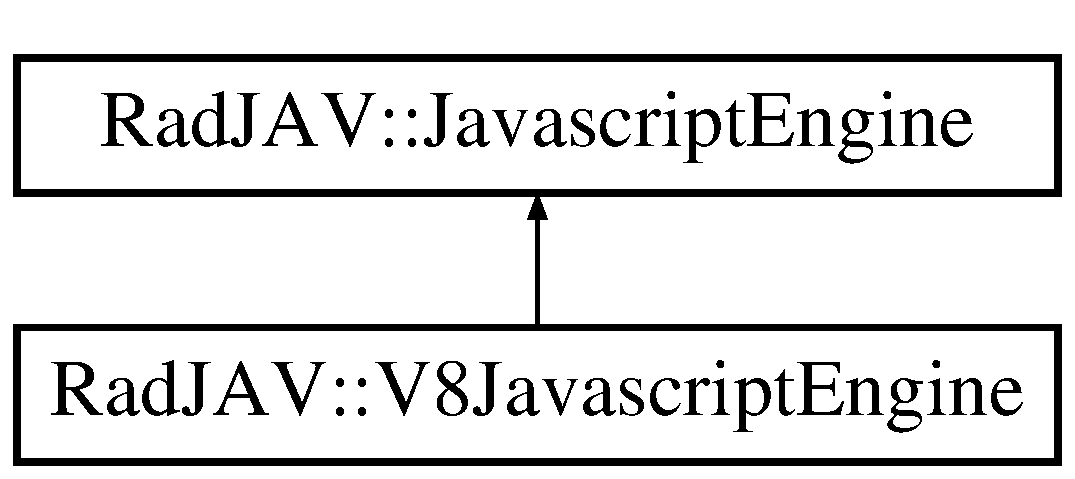
\includegraphics[height=2.000000cm]{class_rad_j_a_v_1_1_javascript_engine}
\end{center}
\end{figure}
\subsection*{Public Member Functions}
\begin{DoxyCompactItemize}
\item 
\mbox{\hyperlink{class_rad_j_a_v_1_1_javascript_engine_a148c454c66e90614abbc589e715b3f7c}{Javascript\+Engine}} ()
\item 
virtual void \mbox{\hyperlink{class_rad_j_a_v_1_1_javascript_engine_a11cc903f042db2b770183667ee36c6bf}{run\+Application}} (\mbox{\hyperlink{class_rad_j_a_v_1_1_string}{String}} application\+Source, \mbox{\hyperlink{class_rad_j_a_v_1_1_string}{String}} file\+Name)=0
\begin{DoxyCompactList}\small\item\em Run an application. \end{DoxyCompactList}\item 
virtual void \mbox{\hyperlink{class_rad_j_a_v_1_1_javascript_engine_a0a435f458e118a813c95ccb359d546e9}{run\+Application\+From\+File}} (\mbox{\hyperlink{class_rad_j_a_v_1_1_string}{String}} file)=0
\begin{DoxyCompactList}\small\item\em Run an application from a javascript file. \end{DoxyCompactList}\item 
virtual void \mbox{\hyperlink{class_rad_j_a_v_1_1_javascript_engine_a4cdc81e5c398f7f1a2ce3ff45f135792}{execute\+Script}} (\mbox{\hyperlink{class_rad_j_a_v_1_1_string}{String}} code, \mbox{\hyperlink{class_rad_j_a_v_1_1_string}{String}} file\+Name)=0
\begin{DoxyCompactList}\small\item\em Execute Javascript code. \end{DoxyCompactList}\item 
virtual void \mbox{\hyperlink{class_rad_j_a_v_1_1_javascript_engine_a91b208b07958c50ce906cd9f25eed669}{load\+Native\+Code}} ()=0
\begin{DoxyCompactList}\small\item\em Connect the native library to the Javascript library. \end{DoxyCompactList}\item 
virtual void \mbox{\hyperlink{class_rad_j_a_v_1_1_javascript_engine_a07709e2f1afb9f49444c6605a7a6122f}{collect\+Garbage}} ()=0
\begin{DoxyCompactList}\small\item\em Call the garbage collector. \end{DoxyCompactList}\item 
virtual void \mbox{\hyperlink{class_rad_j_a_v_1_1_javascript_engine_a76c00d87d65f69781e2dc4aa3143acac}{start3\+D\+Engine}} ()=0
\begin{DoxyCompactList}\small\item\em Start the 3d engine. \end{DoxyCompactList}\item 
virtual void \mbox{\hyperlink{class_rad_j_a_v_1_1_javascript_engine_a91ebe8029a9658f66d9c39356eea2d80}{blockchain\+Event}} (\mbox{\hyperlink{class_rad_j_a_v_1_1_string}{String}} event, \mbox{\hyperlink{class_rad_j_a_v_1_1_string}{String}} data\+Type=\char`\"{}null\char`\"{}, void $\ast$data=N\+U\+LL)=0
\begin{DoxyCompactList}\small\item\em A blockchain event has occurred, process it. \end{DoxyCompactList}\item 
virtual void \mbox{\hyperlink{class_rad_j_a_v_1_1_javascript_engine_abfbd3bff5d4eb0e36d3d18347495bbd7}{add\+Thread}} (\mbox{\hyperlink{class_rad_j_a_v_1_1_thread}{Thread}} $\ast$thread)=0
\begin{DoxyCompactList}\small\item\em Add a thread to be handled by the engine. \end{DoxyCompactList}\item 
virtual void \mbox{\hyperlink{class_rad_j_a_v_1_1_javascript_engine_afe08c6324e3958a5d3ec82fa9e0f1fd1}{remove\+Thread}} (\mbox{\hyperlink{class_rad_j_a_v_1_1_thread}{Thread}} $\ast$thread)=0
\begin{DoxyCompactList}\small\item\em Remove a thread. \end{DoxyCompactList}\item 
virtual void \mbox{\hyperlink{class_rad_j_a_v_1_1_javascript_engine_ab9f13c1928d6967122d0f9a6a026dc73}{throw\+Exception}} (\mbox{\hyperlink{class_rad_j_a_v_1_1_string}{String}} message)=0
\begin{DoxyCompactList}\small\item\em Throw a Javascript exception. \end{DoxyCompactList}\item 
virtual void \mbox{\hyperlink{class_rad_j_a_v_1_1_javascript_engine_a4a720b2e36ab737ab0b697e9b7317fb0}{exit}} (R\+J\+I\+NT exit\+Code)=0
\begin{DoxyCompactList}\small\item\em Shutdown the application entirely. \end{DoxyCompactList}\end{DoxyCompactItemize}
\subsection*{Public Attributes}
\begin{DoxyCompactItemize}
\item 
Ogre\+::\+Root $\ast$ \mbox{\hyperlink{class_rad_j_a_v_1_1_javascript_engine_af494f1d171ea6dbdcccdee1d03f0ca4e}{m\+Root}}
\end{DoxyCompactItemize}
\subsection*{Protected Attributes}
\begin{DoxyCompactItemize}
\item 
R\+J\+B\+O\+OL \mbox{\hyperlink{class_rad_j_a_v_1_1_javascript_engine_ab9d5626eb48dd87bba44eb8db6628cc4}{expose\+GC}}
\item 
R\+J\+B\+O\+OL \mbox{\hyperlink{class_rad_j_a_v_1_1_javascript_engine_ad24ee9119907ff362ac00f7394c665d8}{shutdown\+On\+Exception}}
\item 
R\+J\+B\+O\+OL \mbox{\hyperlink{class_rad_j_a_v_1_1_javascript_engine_ae32ec13d271fa8e9de7076bf19de5fae}{exceptions\+Display\+Message\+Box}}
\item 
R\+J\+B\+O\+OL \mbox{\hyperlink{class_rad_j_a_v_1_1_javascript_engine_a119dba6e5ced56e7c242129993b94556}{shutdown}}
\item 
R\+J\+B\+O\+OL \mbox{\hyperlink{class_rad_j_a_v_1_1_javascript_engine_a64acee3048eba4322c648cad00bc200e}{use\+Debugger}}
\item 
\mbox{\hyperlink{class_rad_j_a_v_1_1_array}{Array}}$<$ R\+J\+U\+L\+O\+NG $>$ \mbox{\hyperlink{class_rad_j_a_v_1_1_javascript_engine_aef0c33700408735d821031b2bcdc77cc}{remove\+Threads}}
\item 
\mbox{\hyperlink{namespace_rad_j_a_v_a7c83af3095bdd8035fd71ff008120f08}{Hash\+Map}}$<$ R\+J\+U\+L\+O\+NG, \mbox{\hyperlink{class_rad_j_a_v_1_1_thread}{Thread}} $\ast$ $>$ \mbox{\hyperlink{class_rad_j_a_v_1_1_javascript_engine_a5ed20d1c0b0bfa1608b5991c71dfd5e9}{threads}}
\end{DoxyCompactItemize}


\subsection{Detailed Description}
The javascript engine to be used. 

\subsection{Constructor \& Destructor Documentation}
\mbox{\Hypertarget{class_rad_j_a_v_1_1_javascript_engine_a148c454c66e90614abbc589e715b3f7c}\label{class_rad_j_a_v_1_1_javascript_engine_a148c454c66e90614abbc589e715b3f7c}} 
\index{Rad\+J\+A\+V\+::\+Javascript\+Engine@{Rad\+J\+A\+V\+::\+Javascript\+Engine}!Javascript\+Engine@{Javascript\+Engine}}
\index{Javascript\+Engine@{Javascript\+Engine}!Rad\+J\+A\+V\+::\+Javascript\+Engine@{Rad\+J\+A\+V\+::\+Javascript\+Engine}}
\subsubsection{\texorpdfstring{Javascript\+Engine()}{JavascriptEngine()}}
{\footnotesize\ttfamily Rad\+J\+A\+V\+::\+Javascript\+Engine\+::\+Javascript\+Engine (\begin{DoxyParamCaption}{ }\end{DoxyParamCaption})\hspace{0.3cm}{\ttfamily [inline]}}



\subsection{Member Function Documentation}
\mbox{\Hypertarget{class_rad_j_a_v_1_1_javascript_engine_abfbd3bff5d4eb0e36d3d18347495bbd7}\label{class_rad_j_a_v_1_1_javascript_engine_abfbd3bff5d4eb0e36d3d18347495bbd7}} 
\index{Rad\+J\+A\+V\+::\+Javascript\+Engine@{Rad\+J\+A\+V\+::\+Javascript\+Engine}!add\+Thread@{add\+Thread}}
\index{add\+Thread@{add\+Thread}!Rad\+J\+A\+V\+::\+Javascript\+Engine@{Rad\+J\+A\+V\+::\+Javascript\+Engine}}
\subsubsection{\texorpdfstring{add\+Thread()}{addThread()}}
{\footnotesize\ttfamily virtual void Rad\+J\+A\+V\+::\+Javascript\+Engine\+::add\+Thread (\begin{DoxyParamCaption}\item[{\mbox{\hyperlink{class_rad_j_a_v_1_1_thread}{Thread}} $\ast$}]{thread }\end{DoxyParamCaption})\hspace{0.3cm}{\ttfamily [pure virtual]}}



Add a thread to be handled by the engine. 



Implemented in \mbox{\hyperlink{class_rad_j_a_v_1_1_v8_javascript_engine_ab72b1bfbf3740039b0ae00008a5e4dd3}{Rad\+J\+A\+V\+::\+V8\+Javascript\+Engine}}.

\mbox{\Hypertarget{class_rad_j_a_v_1_1_javascript_engine_a91ebe8029a9658f66d9c39356eea2d80}\label{class_rad_j_a_v_1_1_javascript_engine_a91ebe8029a9658f66d9c39356eea2d80}} 
\index{Rad\+J\+A\+V\+::\+Javascript\+Engine@{Rad\+J\+A\+V\+::\+Javascript\+Engine}!blockchain\+Event@{blockchain\+Event}}
\index{blockchain\+Event@{blockchain\+Event}!Rad\+J\+A\+V\+::\+Javascript\+Engine@{Rad\+J\+A\+V\+::\+Javascript\+Engine}}
\subsubsection{\texorpdfstring{blockchain\+Event()}{blockchainEvent()}}
{\footnotesize\ttfamily virtual void Rad\+J\+A\+V\+::\+Javascript\+Engine\+::blockchain\+Event (\begin{DoxyParamCaption}\item[{\mbox{\hyperlink{class_rad_j_a_v_1_1_string}{String}}}]{event,  }\item[{\mbox{\hyperlink{class_rad_j_a_v_1_1_string}{String}}}]{data\+Type = {\ttfamily \char`\"{}null\char`\"{}},  }\item[{void $\ast$}]{data = {\ttfamily NULL} }\end{DoxyParamCaption})\hspace{0.3cm}{\ttfamily [pure virtual]}}



A blockchain event has occurred, process it. 



Implemented in \mbox{\hyperlink{class_rad_j_a_v_1_1_v8_javascript_engine_a13490748bc843ae2d2be22aa889e8e30}{Rad\+J\+A\+V\+::\+V8\+Javascript\+Engine}}.

\mbox{\Hypertarget{class_rad_j_a_v_1_1_javascript_engine_a07709e2f1afb9f49444c6605a7a6122f}\label{class_rad_j_a_v_1_1_javascript_engine_a07709e2f1afb9f49444c6605a7a6122f}} 
\index{Rad\+J\+A\+V\+::\+Javascript\+Engine@{Rad\+J\+A\+V\+::\+Javascript\+Engine}!collect\+Garbage@{collect\+Garbage}}
\index{collect\+Garbage@{collect\+Garbage}!Rad\+J\+A\+V\+::\+Javascript\+Engine@{Rad\+J\+A\+V\+::\+Javascript\+Engine}}
\subsubsection{\texorpdfstring{collect\+Garbage()}{collectGarbage()}}
{\footnotesize\ttfamily virtual void Rad\+J\+A\+V\+::\+Javascript\+Engine\+::collect\+Garbage (\begin{DoxyParamCaption}{ }\end{DoxyParamCaption})\hspace{0.3cm}{\ttfamily [pure virtual]}}



Call the garbage collector. 



Implemented in \mbox{\hyperlink{class_rad_j_a_v_1_1_v8_javascript_engine_ab9624aca14bbbcb2bb248d81efe8e402}{Rad\+J\+A\+V\+::\+V8\+Javascript\+Engine}}.

\mbox{\Hypertarget{class_rad_j_a_v_1_1_javascript_engine_a4cdc81e5c398f7f1a2ce3ff45f135792}\label{class_rad_j_a_v_1_1_javascript_engine_a4cdc81e5c398f7f1a2ce3ff45f135792}} 
\index{Rad\+J\+A\+V\+::\+Javascript\+Engine@{Rad\+J\+A\+V\+::\+Javascript\+Engine}!execute\+Script@{execute\+Script}}
\index{execute\+Script@{execute\+Script}!Rad\+J\+A\+V\+::\+Javascript\+Engine@{Rad\+J\+A\+V\+::\+Javascript\+Engine}}
\subsubsection{\texorpdfstring{execute\+Script()}{executeScript()}}
{\footnotesize\ttfamily virtual void Rad\+J\+A\+V\+::\+Javascript\+Engine\+::execute\+Script (\begin{DoxyParamCaption}\item[{\mbox{\hyperlink{class_rad_j_a_v_1_1_string}{String}}}]{code,  }\item[{\mbox{\hyperlink{class_rad_j_a_v_1_1_string}{String}}}]{file\+Name }\end{DoxyParamCaption})\hspace{0.3cm}{\ttfamily [pure virtual]}}



Execute Javascript code. 



Implemented in \mbox{\hyperlink{class_rad_j_a_v_1_1_v8_javascript_engine_ac45d45c9a25fe8f0f9e90fe21e8ef035}{Rad\+J\+A\+V\+::\+V8\+Javascript\+Engine}}.

\mbox{\Hypertarget{class_rad_j_a_v_1_1_javascript_engine_a4a720b2e36ab737ab0b697e9b7317fb0}\label{class_rad_j_a_v_1_1_javascript_engine_a4a720b2e36ab737ab0b697e9b7317fb0}} 
\index{Rad\+J\+A\+V\+::\+Javascript\+Engine@{Rad\+J\+A\+V\+::\+Javascript\+Engine}!exit@{exit}}
\index{exit@{exit}!Rad\+J\+A\+V\+::\+Javascript\+Engine@{Rad\+J\+A\+V\+::\+Javascript\+Engine}}
\subsubsection{\texorpdfstring{exit()}{exit()}}
{\footnotesize\ttfamily virtual void Rad\+J\+A\+V\+::\+Javascript\+Engine\+::exit (\begin{DoxyParamCaption}\item[{R\+J\+I\+NT}]{exit\+Code }\end{DoxyParamCaption})\hspace{0.3cm}{\ttfamily [pure virtual]}}



Shutdown the application entirely. 



Implemented in \mbox{\hyperlink{class_rad_j_a_v_1_1_v8_javascript_engine_a23fcc70cb6805867951748fd1c9706f1}{Rad\+J\+A\+V\+::\+V8\+Javascript\+Engine}}.

\mbox{\Hypertarget{class_rad_j_a_v_1_1_javascript_engine_a91b208b07958c50ce906cd9f25eed669}\label{class_rad_j_a_v_1_1_javascript_engine_a91b208b07958c50ce906cd9f25eed669}} 
\index{Rad\+J\+A\+V\+::\+Javascript\+Engine@{Rad\+J\+A\+V\+::\+Javascript\+Engine}!load\+Native\+Code@{load\+Native\+Code}}
\index{load\+Native\+Code@{load\+Native\+Code}!Rad\+J\+A\+V\+::\+Javascript\+Engine@{Rad\+J\+A\+V\+::\+Javascript\+Engine}}
\subsubsection{\texorpdfstring{load\+Native\+Code()}{loadNativeCode()}}
{\footnotesize\ttfamily virtual void Rad\+J\+A\+V\+::\+Javascript\+Engine\+::load\+Native\+Code (\begin{DoxyParamCaption}{ }\end{DoxyParamCaption})\hspace{0.3cm}{\ttfamily [pure virtual]}}



Connect the native library to the Javascript library. 



Implemented in \mbox{\hyperlink{class_rad_j_a_v_1_1_v8_javascript_engine_afd8d4baa780d5ee7a77754eb5ca52e4d}{Rad\+J\+A\+V\+::\+V8\+Javascript\+Engine}}.

\mbox{\Hypertarget{class_rad_j_a_v_1_1_javascript_engine_afe08c6324e3958a5d3ec82fa9e0f1fd1}\label{class_rad_j_a_v_1_1_javascript_engine_afe08c6324e3958a5d3ec82fa9e0f1fd1}} 
\index{Rad\+J\+A\+V\+::\+Javascript\+Engine@{Rad\+J\+A\+V\+::\+Javascript\+Engine}!remove\+Thread@{remove\+Thread}}
\index{remove\+Thread@{remove\+Thread}!Rad\+J\+A\+V\+::\+Javascript\+Engine@{Rad\+J\+A\+V\+::\+Javascript\+Engine}}
\subsubsection{\texorpdfstring{remove\+Thread()}{removeThread()}}
{\footnotesize\ttfamily virtual void Rad\+J\+A\+V\+::\+Javascript\+Engine\+::remove\+Thread (\begin{DoxyParamCaption}\item[{\mbox{\hyperlink{class_rad_j_a_v_1_1_thread}{Thread}} $\ast$}]{thread }\end{DoxyParamCaption})\hspace{0.3cm}{\ttfamily [pure virtual]}}



Remove a thread. 



Implemented in \mbox{\hyperlink{class_rad_j_a_v_1_1_v8_javascript_engine_a90a52c8c7d655d2e8e5e682d7618c2ab}{Rad\+J\+A\+V\+::\+V8\+Javascript\+Engine}}.

\mbox{\Hypertarget{class_rad_j_a_v_1_1_javascript_engine_a11cc903f042db2b770183667ee36c6bf}\label{class_rad_j_a_v_1_1_javascript_engine_a11cc903f042db2b770183667ee36c6bf}} 
\index{Rad\+J\+A\+V\+::\+Javascript\+Engine@{Rad\+J\+A\+V\+::\+Javascript\+Engine}!run\+Application@{run\+Application}}
\index{run\+Application@{run\+Application}!Rad\+J\+A\+V\+::\+Javascript\+Engine@{Rad\+J\+A\+V\+::\+Javascript\+Engine}}
\subsubsection{\texorpdfstring{run\+Application()}{runApplication()}}
{\footnotesize\ttfamily virtual void Rad\+J\+A\+V\+::\+Javascript\+Engine\+::run\+Application (\begin{DoxyParamCaption}\item[{\mbox{\hyperlink{class_rad_j_a_v_1_1_string}{String}}}]{application\+Source,  }\item[{\mbox{\hyperlink{class_rad_j_a_v_1_1_string}{String}}}]{file\+Name }\end{DoxyParamCaption})\hspace{0.3cm}{\ttfamily [pure virtual]}}



Run an application. 



Implemented in \mbox{\hyperlink{class_rad_j_a_v_1_1_v8_javascript_engine_af792154ac1ceaa6c65faf2409cea5014}{Rad\+J\+A\+V\+::\+V8\+Javascript\+Engine}}.

\mbox{\Hypertarget{class_rad_j_a_v_1_1_javascript_engine_a0a435f458e118a813c95ccb359d546e9}\label{class_rad_j_a_v_1_1_javascript_engine_a0a435f458e118a813c95ccb359d546e9}} 
\index{Rad\+J\+A\+V\+::\+Javascript\+Engine@{Rad\+J\+A\+V\+::\+Javascript\+Engine}!run\+Application\+From\+File@{run\+Application\+From\+File}}
\index{run\+Application\+From\+File@{run\+Application\+From\+File}!Rad\+J\+A\+V\+::\+Javascript\+Engine@{Rad\+J\+A\+V\+::\+Javascript\+Engine}}
\subsubsection{\texorpdfstring{run\+Application\+From\+File()}{runApplicationFromFile()}}
{\footnotesize\ttfamily virtual void Rad\+J\+A\+V\+::\+Javascript\+Engine\+::run\+Application\+From\+File (\begin{DoxyParamCaption}\item[{\mbox{\hyperlink{class_rad_j_a_v_1_1_string}{String}}}]{file }\end{DoxyParamCaption})\hspace{0.3cm}{\ttfamily [pure virtual]}}



Run an application from a javascript file. 



Implemented in \mbox{\hyperlink{class_rad_j_a_v_1_1_v8_javascript_engine_aa0d9d2f20abcf434f8986f7417ebcc3e}{Rad\+J\+A\+V\+::\+V8\+Javascript\+Engine}}.

\mbox{\Hypertarget{class_rad_j_a_v_1_1_javascript_engine_a76c00d87d65f69781e2dc4aa3143acac}\label{class_rad_j_a_v_1_1_javascript_engine_a76c00d87d65f69781e2dc4aa3143acac}} 
\index{Rad\+J\+A\+V\+::\+Javascript\+Engine@{Rad\+J\+A\+V\+::\+Javascript\+Engine}!start3\+D\+Engine@{start3\+D\+Engine}}
\index{start3\+D\+Engine@{start3\+D\+Engine}!Rad\+J\+A\+V\+::\+Javascript\+Engine@{Rad\+J\+A\+V\+::\+Javascript\+Engine}}
\subsubsection{\texorpdfstring{start3\+D\+Engine()}{start3DEngine()}}
{\footnotesize\ttfamily virtual void Rad\+J\+A\+V\+::\+Javascript\+Engine\+::start3\+D\+Engine (\begin{DoxyParamCaption}{ }\end{DoxyParamCaption})\hspace{0.3cm}{\ttfamily [pure virtual]}}



Start the 3d engine. 



Implemented in \mbox{\hyperlink{class_rad_j_a_v_1_1_v8_javascript_engine_ae2e4091f33966a1d722690bcd69f2cde}{Rad\+J\+A\+V\+::\+V8\+Javascript\+Engine}}.

\mbox{\Hypertarget{class_rad_j_a_v_1_1_javascript_engine_ab9f13c1928d6967122d0f9a6a026dc73}\label{class_rad_j_a_v_1_1_javascript_engine_ab9f13c1928d6967122d0f9a6a026dc73}} 
\index{Rad\+J\+A\+V\+::\+Javascript\+Engine@{Rad\+J\+A\+V\+::\+Javascript\+Engine}!throw\+Exception@{throw\+Exception}}
\index{throw\+Exception@{throw\+Exception}!Rad\+J\+A\+V\+::\+Javascript\+Engine@{Rad\+J\+A\+V\+::\+Javascript\+Engine}}
\subsubsection{\texorpdfstring{throw\+Exception()}{throwException()}}
{\footnotesize\ttfamily virtual void Rad\+J\+A\+V\+::\+Javascript\+Engine\+::throw\+Exception (\begin{DoxyParamCaption}\item[{\mbox{\hyperlink{class_rad_j_a_v_1_1_string}{String}}}]{message }\end{DoxyParamCaption})\hspace{0.3cm}{\ttfamily [pure virtual]}}



Throw a Javascript exception. 



Implemented in \mbox{\hyperlink{class_rad_j_a_v_1_1_v8_javascript_engine_a08ad9464e2efe78b0c84d32728b12632}{Rad\+J\+A\+V\+::\+V8\+Javascript\+Engine}}.



\subsection{Member Data Documentation}
\mbox{\Hypertarget{class_rad_j_a_v_1_1_javascript_engine_ae32ec13d271fa8e9de7076bf19de5fae}\label{class_rad_j_a_v_1_1_javascript_engine_ae32ec13d271fa8e9de7076bf19de5fae}} 
\index{Rad\+J\+A\+V\+::\+Javascript\+Engine@{Rad\+J\+A\+V\+::\+Javascript\+Engine}!exceptions\+Display\+Message\+Box@{exceptions\+Display\+Message\+Box}}
\index{exceptions\+Display\+Message\+Box@{exceptions\+Display\+Message\+Box}!Rad\+J\+A\+V\+::\+Javascript\+Engine@{Rad\+J\+A\+V\+::\+Javascript\+Engine}}
\subsubsection{\texorpdfstring{exceptions\+Display\+Message\+Box}{exceptionsDisplayMessageBox}}
{\footnotesize\ttfamily R\+J\+B\+O\+OL Rad\+J\+A\+V\+::\+Javascript\+Engine\+::exceptions\+Display\+Message\+Box\hspace{0.3cm}{\ttfamily [protected]}}

\mbox{\Hypertarget{class_rad_j_a_v_1_1_javascript_engine_ab9d5626eb48dd87bba44eb8db6628cc4}\label{class_rad_j_a_v_1_1_javascript_engine_ab9d5626eb48dd87bba44eb8db6628cc4}} 
\index{Rad\+J\+A\+V\+::\+Javascript\+Engine@{Rad\+J\+A\+V\+::\+Javascript\+Engine}!expose\+GC@{expose\+GC}}
\index{expose\+GC@{expose\+GC}!Rad\+J\+A\+V\+::\+Javascript\+Engine@{Rad\+J\+A\+V\+::\+Javascript\+Engine}}
\subsubsection{\texorpdfstring{expose\+GC}{exposeGC}}
{\footnotesize\ttfamily R\+J\+B\+O\+OL Rad\+J\+A\+V\+::\+Javascript\+Engine\+::expose\+GC\hspace{0.3cm}{\ttfamily [protected]}}

\mbox{\Hypertarget{class_rad_j_a_v_1_1_javascript_engine_af494f1d171ea6dbdcccdee1d03f0ca4e}\label{class_rad_j_a_v_1_1_javascript_engine_af494f1d171ea6dbdcccdee1d03f0ca4e}} 
\index{Rad\+J\+A\+V\+::\+Javascript\+Engine@{Rad\+J\+A\+V\+::\+Javascript\+Engine}!m\+Root@{m\+Root}}
\index{m\+Root@{m\+Root}!Rad\+J\+A\+V\+::\+Javascript\+Engine@{Rad\+J\+A\+V\+::\+Javascript\+Engine}}
\subsubsection{\texorpdfstring{m\+Root}{mRoot}}
{\footnotesize\ttfamily Ogre\+::\+Root$\ast$ Rad\+J\+A\+V\+::\+Javascript\+Engine\+::m\+Root}

\mbox{\Hypertarget{class_rad_j_a_v_1_1_javascript_engine_aef0c33700408735d821031b2bcdc77cc}\label{class_rad_j_a_v_1_1_javascript_engine_aef0c33700408735d821031b2bcdc77cc}} 
\index{Rad\+J\+A\+V\+::\+Javascript\+Engine@{Rad\+J\+A\+V\+::\+Javascript\+Engine}!remove\+Threads@{remove\+Threads}}
\index{remove\+Threads@{remove\+Threads}!Rad\+J\+A\+V\+::\+Javascript\+Engine@{Rad\+J\+A\+V\+::\+Javascript\+Engine}}
\subsubsection{\texorpdfstring{remove\+Threads}{removeThreads}}
{\footnotesize\ttfamily \mbox{\hyperlink{class_rad_j_a_v_1_1_array}{Array}}$<$R\+J\+U\+L\+O\+NG$>$ Rad\+J\+A\+V\+::\+Javascript\+Engine\+::remove\+Threads\hspace{0.3cm}{\ttfamily [protected]}}

\mbox{\Hypertarget{class_rad_j_a_v_1_1_javascript_engine_a119dba6e5ced56e7c242129993b94556}\label{class_rad_j_a_v_1_1_javascript_engine_a119dba6e5ced56e7c242129993b94556}} 
\index{Rad\+J\+A\+V\+::\+Javascript\+Engine@{Rad\+J\+A\+V\+::\+Javascript\+Engine}!shutdown@{shutdown}}
\index{shutdown@{shutdown}!Rad\+J\+A\+V\+::\+Javascript\+Engine@{Rad\+J\+A\+V\+::\+Javascript\+Engine}}
\subsubsection{\texorpdfstring{shutdown}{shutdown}}
{\footnotesize\ttfamily R\+J\+B\+O\+OL Rad\+J\+A\+V\+::\+Javascript\+Engine\+::shutdown\hspace{0.3cm}{\ttfamily [protected]}}

\mbox{\Hypertarget{class_rad_j_a_v_1_1_javascript_engine_ad24ee9119907ff362ac00f7394c665d8}\label{class_rad_j_a_v_1_1_javascript_engine_ad24ee9119907ff362ac00f7394c665d8}} 
\index{Rad\+J\+A\+V\+::\+Javascript\+Engine@{Rad\+J\+A\+V\+::\+Javascript\+Engine}!shutdown\+On\+Exception@{shutdown\+On\+Exception}}
\index{shutdown\+On\+Exception@{shutdown\+On\+Exception}!Rad\+J\+A\+V\+::\+Javascript\+Engine@{Rad\+J\+A\+V\+::\+Javascript\+Engine}}
\subsubsection{\texorpdfstring{shutdown\+On\+Exception}{shutdownOnException}}
{\footnotesize\ttfamily R\+J\+B\+O\+OL Rad\+J\+A\+V\+::\+Javascript\+Engine\+::shutdown\+On\+Exception\hspace{0.3cm}{\ttfamily [protected]}}

\mbox{\Hypertarget{class_rad_j_a_v_1_1_javascript_engine_a5ed20d1c0b0bfa1608b5991c71dfd5e9}\label{class_rad_j_a_v_1_1_javascript_engine_a5ed20d1c0b0bfa1608b5991c71dfd5e9}} 
\index{Rad\+J\+A\+V\+::\+Javascript\+Engine@{Rad\+J\+A\+V\+::\+Javascript\+Engine}!threads@{threads}}
\index{threads@{threads}!Rad\+J\+A\+V\+::\+Javascript\+Engine@{Rad\+J\+A\+V\+::\+Javascript\+Engine}}
\subsubsection{\texorpdfstring{threads}{threads}}
{\footnotesize\ttfamily \mbox{\hyperlink{namespace_rad_j_a_v_a7c83af3095bdd8035fd71ff008120f08}{Hash\+Map}}$<$R\+J\+U\+L\+O\+NG, \mbox{\hyperlink{class_rad_j_a_v_1_1_thread}{Thread}} $\ast$$>$ Rad\+J\+A\+V\+::\+Javascript\+Engine\+::threads\hspace{0.3cm}{\ttfamily [protected]}}

\mbox{\Hypertarget{class_rad_j_a_v_1_1_javascript_engine_a64acee3048eba4322c648cad00bc200e}\label{class_rad_j_a_v_1_1_javascript_engine_a64acee3048eba4322c648cad00bc200e}} 
\index{Rad\+J\+A\+V\+::\+Javascript\+Engine@{Rad\+J\+A\+V\+::\+Javascript\+Engine}!use\+Debugger@{use\+Debugger}}
\index{use\+Debugger@{use\+Debugger}!Rad\+J\+A\+V\+::\+Javascript\+Engine@{Rad\+J\+A\+V\+::\+Javascript\+Engine}}
\subsubsection{\texorpdfstring{use\+Debugger}{useDebugger}}
{\footnotesize\ttfamily R\+J\+B\+O\+OL Rad\+J\+A\+V\+::\+Javascript\+Engine\+::use\+Debugger\hspace{0.3cm}{\ttfamily [protected]}}



The documentation for this class was generated from the following file\+:\begin{DoxyCompactItemize}
\item 
include/\+Rad\+Jav/\mbox{\hyperlink{_rad_jav_javascript_engine_8h}{Rad\+Jav\+Javascript\+Engine.\+h}}\end{DoxyCompactItemize}

\hypertarget{class_rad_j_a_v_1_1_lang}{}\section{Rad\+J\+AV\+:\+:Lang Class Reference}
\label{class_rad_j_a_v_1_1_lang}\index{Rad\+J\+A\+V\+::\+Lang@{Rad\+J\+A\+V\+::\+Lang}}


The language to be used.  




{\ttfamily \#include $<$Rad\+Jav\+Lang.\+h$>$}

\subsection*{Public Member Functions}
\begin{DoxyCompactItemize}
\item 
\mbox{\hyperlink{class_rad_j_a_v_1_1_lang_a6ed1ecee6842cf5d4ffa0a5afcc8dbbc}{Lang}} (\mbox{\hyperlink{class_rad_j_a_v_1_1_string}{String}} lang\+Code)
\item 
void \mbox{\hyperlink{class_rad_j_a_v_1_1_lang_a38ebc57271ef3ffc4ed6aec7854360bf}{get\+String}} (\mbox{\hyperlink{class_rad_j_a_v_1_1_string}{String}} key)
\begin{DoxyCompactList}\small\item\em Get a string associated with a key. \end{DoxyCompactList}\end{DoxyCompactItemize}
\subsection*{Protected Attributes}
\begin{DoxyCompactItemize}
\item 
std\+::map$<$ \mbox{\hyperlink{class_rad_j_a_v_1_1_string}{String}}, \mbox{\hyperlink{class_rad_j_a_v_1_1_string}{String}} $>$ \mbox{\hyperlink{class_rad_j_a_v_1_1_lang_ae8341308089ef735fd294bbdd91c2f37}{lang}}
\end{DoxyCompactItemize}


\subsection{Detailed Description}
The language to be used. 

\subsection{Constructor \& Destructor Documentation}
\mbox{\Hypertarget{class_rad_j_a_v_1_1_lang_a6ed1ecee6842cf5d4ffa0a5afcc8dbbc}\label{class_rad_j_a_v_1_1_lang_a6ed1ecee6842cf5d4ffa0a5afcc8dbbc}} 
\index{Rad\+J\+A\+V\+::\+Lang@{Rad\+J\+A\+V\+::\+Lang}!Lang@{Lang}}
\index{Lang@{Lang}!Rad\+J\+A\+V\+::\+Lang@{Rad\+J\+A\+V\+::\+Lang}}
\subsubsection{\texorpdfstring{Lang()}{Lang()}}
{\footnotesize\ttfamily Rad\+J\+A\+V\+::\+Lang\+::\+Lang (\begin{DoxyParamCaption}\item[{\mbox{\hyperlink{class_rad_j_a_v_1_1_string}{String}}}]{lang\+Code }\end{DoxyParamCaption})}



\subsection{Member Function Documentation}
\mbox{\Hypertarget{class_rad_j_a_v_1_1_lang_a38ebc57271ef3ffc4ed6aec7854360bf}\label{class_rad_j_a_v_1_1_lang_a38ebc57271ef3ffc4ed6aec7854360bf}} 
\index{Rad\+J\+A\+V\+::\+Lang@{Rad\+J\+A\+V\+::\+Lang}!get\+String@{get\+String}}
\index{get\+String@{get\+String}!Rad\+J\+A\+V\+::\+Lang@{Rad\+J\+A\+V\+::\+Lang}}
\subsubsection{\texorpdfstring{get\+String()}{getString()}}
{\footnotesize\ttfamily void Rad\+J\+A\+V\+::\+Lang\+::get\+String (\begin{DoxyParamCaption}\item[{\mbox{\hyperlink{class_rad_j_a_v_1_1_string}{String}}}]{key }\end{DoxyParamCaption})}



Get a string associated with a key. 



\subsection{Member Data Documentation}
\mbox{\Hypertarget{class_rad_j_a_v_1_1_lang_ae8341308089ef735fd294bbdd91c2f37}\label{class_rad_j_a_v_1_1_lang_ae8341308089ef735fd294bbdd91c2f37}} 
\index{Rad\+J\+A\+V\+::\+Lang@{Rad\+J\+A\+V\+::\+Lang}!lang@{lang}}
\index{lang@{lang}!Rad\+J\+A\+V\+::\+Lang@{Rad\+J\+A\+V\+::\+Lang}}
\subsubsection{\texorpdfstring{lang}{lang}}
{\footnotesize\ttfamily std\+::map$<$\mbox{\hyperlink{class_rad_j_a_v_1_1_string}{String}}, \mbox{\hyperlink{class_rad_j_a_v_1_1_string}{String}}$>$ Rad\+J\+A\+V\+::\+Lang\+::lang\hspace{0.3cm}{\ttfamily [protected]}}



The documentation for this class was generated from the following files\+:\begin{DoxyCompactItemize}
\item 
include/\+Rad\+Jav/\mbox{\hyperlink{_rad_jav_lang_8h}{Rad\+Jav\+Lang.\+h}}\item 
src/\+Rad\+Jav/\mbox{\hyperlink{_rad_jav_lang_8cpp}{Rad\+Jav\+Lang.\+cpp}}\end{DoxyCompactItemize}

\hypertarget{class_rad_j_a_v_1_1_rad_jav}{}\section{Rad\+J\+AV\+:\+:Rad\+Jav Class Reference}
\label{class_rad_j_a_v_1_1_rad_jav}\index{Rad\+J\+A\+V\+::\+Rad\+Jav@{Rad\+J\+A\+V\+::\+Rad\+Jav}}


The main \mbox{\hyperlink{class_rad_j_a_v_1_1_rad_jav}{Rad\+Jav}} class, this class handles most if not all functionality.  




{\ttfamily \#include $<$Rad\+Jav.\+h$>$}

\subsection*{Static Public Member Functions}
\begin{DoxyCompactItemize}
\item 
static \mbox{\hyperlink{namespace_rad_j_a_v_a74e0b9a4c586a0346af4029e5a7e3d30}{Rad\+Jav\+Type}} \mbox{\hyperlink{class_rad_j_a_v_1_1_rad_jav_a04f3d51b1f677d8a832696a7f5b4bc6e}{initialize}} (\mbox{\hyperlink{class_rad_j_a_v_1_1_array}{Array}}$<$ \mbox{\hyperlink{class_rad_j_a_v_1_1_string}{String}} $>$ new\+Args, \mbox{\hyperlink{class_rad_j_a_v_1_1wx_widgets_rad_jav}{wx\+Widgets\+Rad\+Jav}} $\ast$new\+App=N\+U\+LL, bool initialize\+Wx\+Widgets=true)
\begin{DoxyCompactList}\small\item\em Start \mbox{\hyperlink{class_rad_j_a_v_1_1_rad_jav}{Rad\+Jav}}. \end{DoxyCompactList}\item 
static \mbox{\hyperlink{class_rad_j_a_v_1_1wx_widgets_rad_jav}{wx\+Widgets\+Rad\+Jav}} $\ast$ \mbox{\hyperlink{class_rad_j_a_v_1_1_rad_jav_a524921ac787c2c33cd9d76e6f89bac67}{getwx\+Widgets\+App}} ()
\begin{DoxyCompactList}\small\item\em Get the wx\+Widgets system. \end{DoxyCompactList}\item 
static \mbox{\hyperlink{namespace_rad_j_a_v_a74e0b9a4c586a0346af4029e5a7e3d30}{Rad\+Jav\+Type}} \mbox{\hyperlink{class_rad_j_a_v_1_1_rad_jav_a0403392e138a7a7ed4b486fc881a1322}{initialize}} (\mbox{\hyperlink{class_rad_j_a_v_1_1_array}{Array}}$<$ \mbox{\hyperlink{class_rad_j_a_v_1_1_string}{String}} $>$ new\+Args)
\begin{DoxyCompactList}\small\item\em Start \mbox{\hyperlink{class_rad_j_a_v_1_1_rad_jav}{Rad\+Jav}}. \end{DoxyCompactList}\item 
static void \mbox{\hyperlink{class_rad_j_a_v_1_1_rad_jav_af1824373c48cbb29dcf9e6047ec97d78}{setup\+Console\+Output}} ()
\begin{DoxyCompactList}\small\item\em Setup console output. \end{DoxyCompactList}\item 
static void \mbox{\hyperlink{class_rad_j_a_v_1_1_rad_jav_aee26bfc80b2d79f1fd8f1be00078dae9}{run\+Event\+Loop}} ()
\begin{DoxyCompactList}\small\item\em Run the event loop indefinitely. \end{DoxyCompactList}\item 
static void \mbox{\hyperlink{class_rad_j_a_v_1_1_rad_jav_a59eb027192379f310cbc66db108b075f}{run\+Event\+Loop\+Single\+Step}} ()
\begin{DoxyCompactList}\small\item\em Run a single step in the event loop. \end{DoxyCompactList}\item 
static void \mbox{\hyperlink{class_rad_j_a_v_1_1_rad_jav_a6dabcf8258dfb10b1c9a785e20add79c}{shutdown}} ()
\begin{DoxyCompactList}\small\item\em Shut down and stop all applications. \end{DoxyCompactList}\item 
static void \mbox{\hyperlink{class_rad_j_a_v_1_1_rad_jav_a7e80e2833cf8f3e223659f0ef3f270ab}{run\+Application}} (\mbox{\hyperlink{class_rad_j_a_v_1_1_string}{String}} application, \mbox{\hyperlink{class_rad_j_a_v_1_1_string}{String}} file\+Name)
\begin{DoxyCompactList}\small\item\em Run an application. \end{DoxyCompactList}\item 
static void \mbox{\hyperlink{class_rad_j_a_v_1_1_rad_jav_a293b050fb802c1d1c1112895388c9c7c}{run\+Application\+From\+File}} (\mbox{\hyperlink{class_rad_j_a_v_1_1_string}{String}} file)
\begin{DoxyCompactList}\small\item\em Run an application from a javascript file. \end{DoxyCompactList}\item 
static void \mbox{\hyperlink{class_rad_j_a_v_1_1_rad_jav_a70ed4cb4f4b341770046193fcf5118dd}{show\+Message\+Box}} (\mbox{\hyperlink{class_rad_j_a_v_1_1_string}{String}} message, \mbox{\hyperlink{class_rad_j_a_v_1_1_string}{String}} title)
\begin{DoxyCompactList}\small\item\em Show a message box. \end{DoxyCompactList}\item 
static void \mbox{\hyperlink{class_rad_j_a_v_1_1_rad_jav_ab91e1d55577183ed105e393c06df6374}{show\+Error}} (\mbox{\hyperlink{class_rad_j_a_v_1_1_string}{String}} message, R\+J\+B\+O\+OL \mbox{\hyperlink{class_rad_j_a_v_1_1_rad_jav_a70ed4cb4f4b341770046193fcf5118dd}{show\+Message\+Box}}=false)
\begin{DoxyCompactList}\small\item\em Show an error message. \end{DoxyCompactList}\item 
static void \mbox{\hyperlink{class_rad_j_a_v_1_1_rad_jav_aa06bae2f115631a90a2426d818499049}{print\+To\+Output\+Window}} (\mbox{\hyperlink{class_rad_j_a_v_1_1_string}{String}} message)
\item 
static void \mbox{\hyperlink{class_rad_j_a_v_1_1_rad_jav_a0f461b48e84744a69df4ff30dbf7d302}{log\+New\+Memory\+Alloc}} (\mbox{\hyperlink{class_rad_j_a_v_1_1_memory_alloc_log}{Memory\+Alloc\+Log}} alloc)
\item 
static void \mbox{\hyperlink{class_rad_j_a_v_1_1_rad_jav_a6226fe15f13446edc493596b6c029cb7}{remove\+Memory\+Alloc}} (\mbox{\hyperlink{class_rad_j_a_v_1_1_memory_alloc_log}{Memory\+Alloc\+Log}} alloc)
\item 
static \mbox{\hyperlink{class_rad_j_a_v_1_1_string}{String}} \mbox{\hyperlink{class_rad_j_a_v_1_1_rad_jav_a26e6e428425568f87a7ac59e2eef5359}{report\+Memory\+Leaks}} ()
\end{DoxyCompactItemize}
\subsection*{Static Public Attributes}
\begin{DoxyCompactItemize}
\item 
static \mbox{\hyperlink{class_rad_j_a_v_1_1_lang}{Lang}} $\ast$ \mbox{\hyperlink{class_rad_j_a_v_1_1_rad_jav_ac27c2fc21e98d8961c7e98099b71c4f3}{lang}} = N\+U\+LL
\begin{DoxyCompactList}\small\item\em Handles strings from languages. \end{DoxyCompactList}\item 
static \mbox{\hyperlink{class_rad_j_a_v_1_1_theme}{Theme}} $\ast$ \mbox{\hyperlink{class_rad_j_a_v_1_1_rad_jav_ace6c4f9cb9d0d9c248986feeea31150e}{theme}} = N\+U\+LL
\begin{DoxyCompactList}\small\item\em Handles the loaded \mbox{\hyperlink{class_rad_j_a_v_1_1_theme}{Theme}}. \end{DoxyCompactList}\item 
static \mbox{\hyperlink{class_rad_j_a_v_1_1wx_widgets_rad_jav}{wx\+Widgets\+Rad\+Jav}} $\ast$ \mbox{\hyperlink{class_rad_j_a_v_1_1_rad_jav_aa7084f6f5e9bfddf213a16c06878cb36}{app}} = N\+U\+LL
\begin{DoxyCompactList}\small\item\em The \mbox{\hyperlink{namespace_rad_j_a_v_1_1_g_u_i}{G\+UI}} system used to display the \mbox{\hyperlink{namespace_rad_j_a_v_1_1_g_u_i}{G\+UI}}. \end{DoxyCompactList}\item 
static \mbox{\hyperlink{class_rad_j_a_v_1_1_javascript_engine}{Javascript\+Engine}} $\ast$ \mbox{\hyperlink{class_rad_j_a_v_1_1_rad_jav_aa80128a74f47d969173d2e7946e0ae6c}{javascript\+Engine}} = N\+U\+LL
\begin{DoxyCompactList}\small\item\em The javascript engine used to execute applications. \end{DoxyCompactList}\item 
static \mbox{\hyperlink{class_rad_j_a_v_1_1_array}{Array}}$<$ \mbox{\hyperlink{class_rad_j_a_v_1_1_string}{String}} $>$ \mbox{\hyperlink{class_rad_j_a_v_1_1_rad_jav_a8a4b1ccb076b4ffa84b285d8c1d1e050}{arguments}}
\begin{DoxyCompactList}\small\item\em The command line arguments used to start \mbox{\hyperlink{class_rad_j_a_v_1_1_rad_jav}{Rad\+Jav}}. \end{DoxyCompactList}\item 
static \mbox{\hyperlink{namespace_rad_j_a_v_a7c83af3095bdd8035fd71ff008120f08}{Hash\+Map}}$<$ size\+\_\+t, \mbox{\hyperlink{class_rad_j_a_v_1_1_memory_alloc_log}{Memory\+Alloc\+Log}} $>$ \mbox{\hyperlink{class_rad_j_a_v_1_1_rad_jav_abb9c47c4a37be67599ee136f9fbbd33e}{memory\+Allocs}}
\begin{DoxyCompactList}\small\item\em Memory allocations made during debug. \end{DoxyCompactList}\end{DoxyCompactItemize}


\subsection{Detailed Description}
The main \mbox{\hyperlink{class_rad_j_a_v_1_1_rad_jav}{Rad\+Jav}} class, this class handles most if not all functionality. 

\subsection{Member Function Documentation}
\mbox{\Hypertarget{class_rad_j_a_v_1_1_rad_jav_a524921ac787c2c33cd9d76e6f89bac67}\label{class_rad_j_a_v_1_1_rad_jav_a524921ac787c2c33cd9d76e6f89bac67}} 
\index{Rad\+J\+A\+V\+::\+Rad\+Jav@{Rad\+J\+A\+V\+::\+Rad\+Jav}!getwx\+Widgets\+App@{getwx\+Widgets\+App}}
\index{getwx\+Widgets\+App@{getwx\+Widgets\+App}!Rad\+J\+A\+V\+::\+Rad\+Jav@{Rad\+J\+A\+V\+::\+Rad\+Jav}}
\subsubsection{\texorpdfstring{getwx\+Widgets\+App()}{getwxWidgetsApp()}}
{\footnotesize\ttfamily static \mbox{\hyperlink{class_rad_j_a_v_1_1wx_widgets_rad_jav}{wx\+Widgets\+Rad\+Jav}}$\ast$ Rad\+J\+A\+V\+::\+Rad\+Jav\+::getwx\+Widgets\+App (\begin{DoxyParamCaption}{ }\end{DoxyParamCaption})\hspace{0.3cm}{\ttfamily [inline]}, {\ttfamily [static]}}



Get the wx\+Widgets system. 

\mbox{\Hypertarget{class_rad_j_a_v_1_1_rad_jav_a04f3d51b1f677d8a832696a7f5b4bc6e}\label{class_rad_j_a_v_1_1_rad_jav_a04f3d51b1f677d8a832696a7f5b4bc6e}} 
\index{Rad\+J\+A\+V\+::\+Rad\+Jav@{Rad\+J\+A\+V\+::\+Rad\+Jav}!initialize@{initialize}}
\index{initialize@{initialize}!Rad\+J\+A\+V\+::\+Rad\+Jav@{Rad\+J\+A\+V\+::\+Rad\+Jav}}
\subsubsection{\texorpdfstring{initialize()}{initialize()}\hspace{0.1cm}{\footnotesize\ttfamily [1/2]}}
{\footnotesize\ttfamily \mbox{\hyperlink{namespace_rad_j_a_v_a74e0b9a4c586a0346af4029e5a7e3d30}{Rad\+Jav\+Type}} Rad\+J\+A\+V\+::\+Rad\+Jav\+::initialize (\begin{DoxyParamCaption}\item[{\mbox{\hyperlink{class_rad_j_a_v_1_1_array}{Array}}$<$ \mbox{\hyperlink{class_rad_j_a_v_1_1_string}{String}} $>$}]{new\+Args,  }\item[{\mbox{\hyperlink{class_rad_j_a_v_1_1wx_widgets_rad_jav}{wx\+Widgets\+Rad\+Jav}} $\ast$}]{new\+App = {\ttfamily NULL},  }\item[{bool}]{initialize\+Wx\+Widgets = {\ttfamily true} }\end{DoxyParamCaption})\hspace{0.3cm}{\ttfamily [static]}}



Start \mbox{\hyperlink{class_rad_j_a_v_1_1_rad_jav}{Rad\+Jav}}. 

\mbox{\Hypertarget{class_rad_j_a_v_1_1_rad_jav_a0403392e138a7a7ed4b486fc881a1322}\label{class_rad_j_a_v_1_1_rad_jav_a0403392e138a7a7ed4b486fc881a1322}} 
\index{Rad\+J\+A\+V\+::\+Rad\+Jav@{Rad\+J\+A\+V\+::\+Rad\+Jav}!initialize@{initialize}}
\index{initialize@{initialize}!Rad\+J\+A\+V\+::\+Rad\+Jav@{Rad\+J\+A\+V\+::\+Rad\+Jav}}
\subsubsection{\texorpdfstring{initialize()}{initialize()}\hspace{0.1cm}{\footnotesize\ttfamily [2/2]}}
{\footnotesize\ttfamily \mbox{\hyperlink{namespace_rad_j_a_v_a74e0b9a4c586a0346af4029e5a7e3d30}{Rad\+Jav\+Type}} Rad\+J\+A\+V\+::\+Rad\+Jav\+::initialize (\begin{DoxyParamCaption}\item[{\mbox{\hyperlink{class_rad_j_a_v_1_1_array}{Array}}$<$ \mbox{\hyperlink{class_rad_j_a_v_1_1_string}{String}} $>$}]{new\+Args }\end{DoxyParamCaption})\hspace{0.3cm}{\ttfamily [static]}}



Start \mbox{\hyperlink{class_rad_j_a_v_1_1_rad_jav}{Rad\+Jav}}. 

\mbox{\Hypertarget{class_rad_j_a_v_1_1_rad_jav_a0f461b48e84744a69df4ff30dbf7d302}\label{class_rad_j_a_v_1_1_rad_jav_a0f461b48e84744a69df4ff30dbf7d302}} 
\index{Rad\+J\+A\+V\+::\+Rad\+Jav@{Rad\+J\+A\+V\+::\+Rad\+Jav}!log\+New\+Memory\+Alloc@{log\+New\+Memory\+Alloc}}
\index{log\+New\+Memory\+Alloc@{log\+New\+Memory\+Alloc}!Rad\+J\+A\+V\+::\+Rad\+Jav@{Rad\+J\+A\+V\+::\+Rad\+Jav}}
\subsubsection{\texorpdfstring{log\+New\+Memory\+Alloc()}{logNewMemoryAlloc()}}
{\footnotesize\ttfamily void Rad\+J\+A\+V\+::\+Rad\+Jav\+::log\+New\+Memory\+Alloc (\begin{DoxyParamCaption}\item[{\mbox{\hyperlink{class_rad_j_a_v_1_1_memory_alloc_log}{Memory\+Alloc\+Log}}}]{alloc }\end{DoxyParamCaption})\hspace{0.3cm}{\ttfamily [static]}}

\mbox{\Hypertarget{class_rad_j_a_v_1_1_rad_jav_aa06bae2f115631a90a2426d818499049}\label{class_rad_j_a_v_1_1_rad_jav_aa06bae2f115631a90a2426d818499049}} 
\index{Rad\+J\+A\+V\+::\+Rad\+Jav@{Rad\+J\+A\+V\+::\+Rad\+Jav}!print\+To\+Output\+Window@{print\+To\+Output\+Window}}
\index{print\+To\+Output\+Window@{print\+To\+Output\+Window}!Rad\+J\+A\+V\+::\+Rad\+Jav@{Rad\+J\+A\+V\+::\+Rad\+Jav}}
\subsubsection{\texorpdfstring{print\+To\+Output\+Window()}{printToOutputWindow()}}
{\footnotesize\ttfamily void Rad\+J\+A\+V\+::\+Rad\+Jav\+::print\+To\+Output\+Window (\begin{DoxyParamCaption}\item[{\mbox{\hyperlink{class_rad_j_a_v_1_1_string}{String}}}]{message }\end{DoxyParamCaption})\hspace{0.3cm}{\ttfamily [static]}}

Primarily for Visual Studio debugging. This will print to the output window, or to the console if on another platform. \mbox{\Hypertarget{class_rad_j_a_v_1_1_rad_jav_a6226fe15f13446edc493596b6c029cb7}\label{class_rad_j_a_v_1_1_rad_jav_a6226fe15f13446edc493596b6c029cb7}} 
\index{Rad\+J\+A\+V\+::\+Rad\+Jav@{Rad\+J\+A\+V\+::\+Rad\+Jav}!remove\+Memory\+Alloc@{remove\+Memory\+Alloc}}
\index{remove\+Memory\+Alloc@{remove\+Memory\+Alloc}!Rad\+J\+A\+V\+::\+Rad\+Jav@{Rad\+J\+A\+V\+::\+Rad\+Jav}}
\subsubsection{\texorpdfstring{remove\+Memory\+Alloc()}{removeMemoryAlloc()}}
{\footnotesize\ttfamily void Rad\+J\+A\+V\+::\+Rad\+Jav\+::remove\+Memory\+Alloc (\begin{DoxyParamCaption}\item[{\mbox{\hyperlink{class_rad_j_a_v_1_1_memory_alloc_log}{Memory\+Alloc\+Log}}}]{alloc }\end{DoxyParamCaption})\hspace{0.3cm}{\ttfamily [static]}}

\mbox{\Hypertarget{class_rad_j_a_v_1_1_rad_jav_a26e6e428425568f87a7ac59e2eef5359}\label{class_rad_j_a_v_1_1_rad_jav_a26e6e428425568f87a7ac59e2eef5359}} 
\index{Rad\+J\+A\+V\+::\+Rad\+Jav@{Rad\+J\+A\+V\+::\+Rad\+Jav}!report\+Memory\+Leaks@{report\+Memory\+Leaks}}
\index{report\+Memory\+Leaks@{report\+Memory\+Leaks}!Rad\+J\+A\+V\+::\+Rad\+Jav@{Rad\+J\+A\+V\+::\+Rad\+Jav}}
\subsubsection{\texorpdfstring{report\+Memory\+Leaks()}{reportMemoryLeaks()}}
{\footnotesize\ttfamily \mbox{\hyperlink{class_rad_j_a_v_1_1_string}{String}} Rad\+J\+A\+V\+::\+Rad\+Jav\+::report\+Memory\+Leaks (\begin{DoxyParamCaption}{ }\end{DoxyParamCaption})\hspace{0.3cm}{\ttfamily [static]}}

\mbox{\Hypertarget{class_rad_j_a_v_1_1_rad_jav_a7e80e2833cf8f3e223659f0ef3f270ab}\label{class_rad_j_a_v_1_1_rad_jav_a7e80e2833cf8f3e223659f0ef3f270ab}} 
\index{Rad\+J\+A\+V\+::\+Rad\+Jav@{Rad\+J\+A\+V\+::\+Rad\+Jav}!run\+Application@{run\+Application}}
\index{run\+Application@{run\+Application}!Rad\+J\+A\+V\+::\+Rad\+Jav@{Rad\+J\+A\+V\+::\+Rad\+Jav}}
\subsubsection{\texorpdfstring{run\+Application()}{runApplication()}}
{\footnotesize\ttfamily void Rad\+J\+A\+V\+::\+Rad\+Jav\+::run\+Application (\begin{DoxyParamCaption}\item[{\mbox{\hyperlink{class_rad_j_a_v_1_1_string}{String}}}]{application,  }\item[{\mbox{\hyperlink{class_rad_j_a_v_1_1_string}{String}}}]{file\+Name }\end{DoxyParamCaption})\hspace{0.3cm}{\ttfamily [static]}}



Run an application. 

\mbox{\Hypertarget{class_rad_j_a_v_1_1_rad_jav_a293b050fb802c1d1c1112895388c9c7c}\label{class_rad_j_a_v_1_1_rad_jav_a293b050fb802c1d1c1112895388c9c7c}} 
\index{Rad\+J\+A\+V\+::\+Rad\+Jav@{Rad\+J\+A\+V\+::\+Rad\+Jav}!run\+Application\+From\+File@{run\+Application\+From\+File}}
\index{run\+Application\+From\+File@{run\+Application\+From\+File}!Rad\+J\+A\+V\+::\+Rad\+Jav@{Rad\+J\+A\+V\+::\+Rad\+Jav}}
\subsubsection{\texorpdfstring{run\+Application\+From\+File()}{runApplicationFromFile()}}
{\footnotesize\ttfamily void Rad\+J\+A\+V\+::\+Rad\+Jav\+::run\+Application\+From\+File (\begin{DoxyParamCaption}\item[{\mbox{\hyperlink{class_rad_j_a_v_1_1_string}{String}}}]{file }\end{DoxyParamCaption})\hspace{0.3cm}{\ttfamily [static]}}



Run an application from a javascript file. 

\mbox{\Hypertarget{class_rad_j_a_v_1_1_rad_jav_aee26bfc80b2d79f1fd8f1be00078dae9}\label{class_rad_j_a_v_1_1_rad_jav_aee26bfc80b2d79f1fd8f1be00078dae9}} 
\index{Rad\+J\+A\+V\+::\+Rad\+Jav@{Rad\+J\+A\+V\+::\+Rad\+Jav}!run\+Event\+Loop@{run\+Event\+Loop}}
\index{run\+Event\+Loop@{run\+Event\+Loop}!Rad\+J\+A\+V\+::\+Rad\+Jav@{Rad\+J\+A\+V\+::\+Rad\+Jav}}
\subsubsection{\texorpdfstring{run\+Event\+Loop()}{runEventLoop()}}
{\footnotesize\ttfamily void Rad\+J\+A\+V\+::\+Rad\+Jav\+::run\+Event\+Loop (\begin{DoxyParamCaption}{ }\end{DoxyParamCaption})\hspace{0.3cm}{\ttfamily [static]}}



Run the event loop indefinitely. 

\mbox{\Hypertarget{class_rad_j_a_v_1_1_rad_jav_a59eb027192379f310cbc66db108b075f}\label{class_rad_j_a_v_1_1_rad_jav_a59eb027192379f310cbc66db108b075f}} 
\index{Rad\+J\+A\+V\+::\+Rad\+Jav@{Rad\+J\+A\+V\+::\+Rad\+Jav}!run\+Event\+Loop\+Single\+Step@{run\+Event\+Loop\+Single\+Step}}
\index{run\+Event\+Loop\+Single\+Step@{run\+Event\+Loop\+Single\+Step}!Rad\+J\+A\+V\+::\+Rad\+Jav@{Rad\+J\+A\+V\+::\+Rad\+Jav}}
\subsubsection{\texorpdfstring{run\+Event\+Loop\+Single\+Step()}{runEventLoopSingleStep()}}
{\footnotesize\ttfamily void Rad\+J\+A\+V\+::\+Rad\+Jav\+::run\+Event\+Loop\+Single\+Step (\begin{DoxyParamCaption}{ }\end{DoxyParamCaption})\hspace{0.3cm}{\ttfamily [static]}}



Run a single step in the event loop. 

\mbox{\Hypertarget{class_rad_j_a_v_1_1_rad_jav_af1824373c48cbb29dcf9e6047ec97d78}\label{class_rad_j_a_v_1_1_rad_jav_af1824373c48cbb29dcf9e6047ec97d78}} 
\index{Rad\+J\+A\+V\+::\+Rad\+Jav@{Rad\+J\+A\+V\+::\+Rad\+Jav}!setup\+Console\+Output@{setup\+Console\+Output}}
\index{setup\+Console\+Output@{setup\+Console\+Output}!Rad\+J\+A\+V\+::\+Rad\+Jav@{Rad\+J\+A\+V\+::\+Rad\+Jav}}
\subsubsection{\texorpdfstring{setup\+Console\+Output()}{setupConsoleOutput()}}
{\footnotesize\ttfamily void Rad\+J\+A\+V\+::\+Rad\+Jav\+::setup\+Console\+Output (\begin{DoxyParamCaption}{ }\end{DoxyParamCaption})\hspace{0.3cm}{\ttfamily [static]}}



Setup console output. 

\mbox{\Hypertarget{class_rad_j_a_v_1_1_rad_jav_ab91e1d55577183ed105e393c06df6374}\label{class_rad_j_a_v_1_1_rad_jav_ab91e1d55577183ed105e393c06df6374}} 
\index{Rad\+J\+A\+V\+::\+Rad\+Jav@{Rad\+J\+A\+V\+::\+Rad\+Jav}!show\+Error@{show\+Error}}
\index{show\+Error@{show\+Error}!Rad\+J\+A\+V\+::\+Rad\+Jav@{Rad\+J\+A\+V\+::\+Rad\+Jav}}
\subsubsection{\texorpdfstring{show\+Error()}{showError()}}
{\footnotesize\ttfamily void Rad\+J\+A\+V\+::\+Rad\+Jav\+::show\+Error (\begin{DoxyParamCaption}\item[{\mbox{\hyperlink{class_rad_j_a_v_1_1_string}{String}}}]{message,  }\item[{R\+J\+B\+O\+OL}]{show\+Message\+Box = {\ttfamily false} }\end{DoxyParamCaption})\hspace{0.3cm}{\ttfamily [static]}}



Show an error message. 

\mbox{\Hypertarget{class_rad_j_a_v_1_1_rad_jav_a70ed4cb4f4b341770046193fcf5118dd}\label{class_rad_j_a_v_1_1_rad_jav_a70ed4cb4f4b341770046193fcf5118dd}} 
\index{Rad\+J\+A\+V\+::\+Rad\+Jav@{Rad\+J\+A\+V\+::\+Rad\+Jav}!show\+Message\+Box@{show\+Message\+Box}}
\index{show\+Message\+Box@{show\+Message\+Box}!Rad\+J\+A\+V\+::\+Rad\+Jav@{Rad\+J\+A\+V\+::\+Rad\+Jav}}
\subsubsection{\texorpdfstring{show\+Message\+Box()}{showMessageBox()}}
{\footnotesize\ttfamily void Rad\+J\+A\+V\+::\+Rad\+Jav\+::show\+Message\+Box (\begin{DoxyParamCaption}\item[{\mbox{\hyperlink{class_rad_j_a_v_1_1_string}{String}}}]{message,  }\item[{\mbox{\hyperlink{class_rad_j_a_v_1_1_string}{String}}}]{title }\end{DoxyParamCaption})\hspace{0.3cm}{\ttfamily [static]}}



Show a message box. 

\mbox{\Hypertarget{class_rad_j_a_v_1_1_rad_jav_a6dabcf8258dfb10b1c9a785e20add79c}\label{class_rad_j_a_v_1_1_rad_jav_a6dabcf8258dfb10b1c9a785e20add79c}} 
\index{Rad\+J\+A\+V\+::\+Rad\+Jav@{Rad\+J\+A\+V\+::\+Rad\+Jav}!shutdown@{shutdown}}
\index{shutdown@{shutdown}!Rad\+J\+A\+V\+::\+Rad\+Jav@{Rad\+J\+A\+V\+::\+Rad\+Jav}}
\subsubsection{\texorpdfstring{shutdown()}{shutdown()}}
{\footnotesize\ttfamily void Rad\+J\+A\+V\+::\+Rad\+Jav\+::shutdown (\begin{DoxyParamCaption}{ }\end{DoxyParamCaption})\hspace{0.3cm}{\ttfamily [static]}}



Shut down and stop all applications. 



\subsection{Member Data Documentation}
\mbox{\Hypertarget{class_rad_j_a_v_1_1_rad_jav_aa7084f6f5e9bfddf213a16c06878cb36}\label{class_rad_j_a_v_1_1_rad_jav_aa7084f6f5e9bfddf213a16c06878cb36}} 
\index{Rad\+J\+A\+V\+::\+Rad\+Jav@{Rad\+J\+A\+V\+::\+Rad\+Jav}!app@{app}}
\index{app@{app}!Rad\+J\+A\+V\+::\+Rad\+Jav@{Rad\+J\+A\+V\+::\+Rad\+Jav}}
\subsubsection{\texorpdfstring{app}{app}}
{\footnotesize\ttfamily \mbox{\hyperlink{class_rad_j_a_v_1_1wx_widgets_rad_jav}{wx\+Widgets\+Rad\+Jav}} $\ast$ Rad\+J\+A\+V\+::\+Rad\+Jav\+::app = N\+U\+LL\hspace{0.3cm}{\ttfamily [static]}}



The \mbox{\hyperlink{namespace_rad_j_a_v_1_1_g_u_i}{G\+UI}} system used to display the \mbox{\hyperlink{namespace_rad_j_a_v_1_1_g_u_i}{G\+UI}}. 

\mbox{\Hypertarget{class_rad_j_a_v_1_1_rad_jav_a8a4b1ccb076b4ffa84b285d8c1d1e050}\label{class_rad_j_a_v_1_1_rad_jav_a8a4b1ccb076b4ffa84b285d8c1d1e050}} 
\index{Rad\+J\+A\+V\+::\+Rad\+Jav@{Rad\+J\+A\+V\+::\+Rad\+Jav}!arguments@{arguments}}
\index{arguments@{arguments}!Rad\+J\+A\+V\+::\+Rad\+Jav@{Rad\+J\+A\+V\+::\+Rad\+Jav}}
\subsubsection{\texorpdfstring{arguments}{arguments}}
{\footnotesize\ttfamily \mbox{\hyperlink{class_rad_j_a_v_1_1_array}{Array}}$<$ \mbox{\hyperlink{class_rad_j_a_v_1_1_string}{String}} $>$ Rad\+J\+A\+V\+::\+Rad\+Jav\+::arguments\hspace{0.3cm}{\ttfamily [static]}}



The command line arguments used to start \mbox{\hyperlink{class_rad_j_a_v_1_1_rad_jav}{Rad\+Jav}}. 

\mbox{\Hypertarget{class_rad_j_a_v_1_1_rad_jav_aa80128a74f47d969173d2e7946e0ae6c}\label{class_rad_j_a_v_1_1_rad_jav_aa80128a74f47d969173d2e7946e0ae6c}} 
\index{Rad\+J\+A\+V\+::\+Rad\+Jav@{Rad\+J\+A\+V\+::\+Rad\+Jav}!javascript\+Engine@{javascript\+Engine}}
\index{javascript\+Engine@{javascript\+Engine}!Rad\+J\+A\+V\+::\+Rad\+Jav@{Rad\+J\+A\+V\+::\+Rad\+Jav}}
\subsubsection{\texorpdfstring{javascript\+Engine}{javascriptEngine}}
{\footnotesize\ttfamily \mbox{\hyperlink{class_rad_j_a_v_1_1_javascript_engine}{Javascript\+Engine}} $\ast$ Rad\+J\+A\+V\+::\+Rad\+Jav\+::javascript\+Engine = N\+U\+LL\hspace{0.3cm}{\ttfamily [static]}}



The javascript engine used to execute applications. 

\mbox{\Hypertarget{class_rad_j_a_v_1_1_rad_jav_ac27c2fc21e98d8961c7e98099b71c4f3}\label{class_rad_j_a_v_1_1_rad_jav_ac27c2fc21e98d8961c7e98099b71c4f3}} 
\index{Rad\+J\+A\+V\+::\+Rad\+Jav@{Rad\+J\+A\+V\+::\+Rad\+Jav}!lang@{lang}}
\index{lang@{lang}!Rad\+J\+A\+V\+::\+Rad\+Jav@{Rad\+J\+A\+V\+::\+Rad\+Jav}}
\subsubsection{\texorpdfstring{lang}{lang}}
{\footnotesize\ttfamily \mbox{\hyperlink{class_rad_j_a_v_1_1_lang}{Lang}} $\ast$ Rad\+J\+A\+V\+::\+Rad\+Jav\+::lang = N\+U\+LL\hspace{0.3cm}{\ttfamily [static]}}



Handles strings from languages. 

\mbox{\Hypertarget{class_rad_j_a_v_1_1_rad_jav_abb9c47c4a37be67599ee136f9fbbd33e}\label{class_rad_j_a_v_1_1_rad_jav_abb9c47c4a37be67599ee136f9fbbd33e}} 
\index{Rad\+J\+A\+V\+::\+Rad\+Jav@{Rad\+J\+A\+V\+::\+Rad\+Jav}!memory\+Allocs@{memory\+Allocs}}
\index{memory\+Allocs@{memory\+Allocs}!Rad\+J\+A\+V\+::\+Rad\+Jav@{Rad\+J\+A\+V\+::\+Rad\+Jav}}
\subsubsection{\texorpdfstring{memory\+Allocs}{memoryAllocs}}
{\footnotesize\ttfamily \mbox{\hyperlink{namespace_rad_j_a_v_a7c83af3095bdd8035fd71ff008120f08}{Hash\+Map}}$<$ size\+\_\+t, \mbox{\hyperlink{class_rad_j_a_v_1_1_memory_alloc_log}{Memory\+Alloc\+Log}} $>$ Rad\+J\+A\+V\+::\+Rad\+Jav\+::memory\+Allocs\hspace{0.3cm}{\ttfamily [static]}}



Memory allocations made during debug. 

\mbox{\Hypertarget{class_rad_j_a_v_1_1_rad_jav_ace6c4f9cb9d0d9c248986feeea31150e}\label{class_rad_j_a_v_1_1_rad_jav_ace6c4f9cb9d0d9c248986feeea31150e}} 
\index{Rad\+J\+A\+V\+::\+Rad\+Jav@{Rad\+J\+A\+V\+::\+Rad\+Jav}!theme@{theme}}
\index{theme@{theme}!Rad\+J\+A\+V\+::\+Rad\+Jav@{Rad\+J\+A\+V\+::\+Rad\+Jav}}
\subsubsection{\texorpdfstring{theme}{theme}}
{\footnotesize\ttfamily \mbox{\hyperlink{class_rad_j_a_v_1_1_theme}{Theme}} $\ast$ Rad\+J\+A\+V\+::\+Rad\+Jav\+::theme = N\+U\+LL\hspace{0.3cm}{\ttfamily [static]}}



Handles the loaded \mbox{\hyperlink{class_rad_j_a_v_1_1_theme}{Theme}}. 



The documentation for this class was generated from the following files\+:\begin{DoxyCompactItemize}
\item 
include/\+Rad\+Jav/\mbox{\hyperlink{_rad_jav_8h}{Rad\+Jav.\+h}}\item 
src/\+Rad\+Jav/\mbox{\hyperlink{_rad_jav_8cpp}{Rad\+Jav.\+cpp}}\end{DoxyCompactItemize}

\hypertarget{class_rad_j_a_v_1_1_rectangle}{}\section{Rad\+J\+AV\+:\+:Rectangle Class Reference}
\label{class_rad_j_a_v_1_1_rectangle}\index{Rad\+J\+A\+V\+::\+Rectangle@{Rad\+J\+A\+V\+::\+Rectangle}}


{\ttfamily \#include $<$Rad\+Jav\+Rectangle.\+h$>$}

\subsection*{Public Member Functions}
\begin{DoxyCompactItemize}
\item 
\hyperlink{class_rad_j_a_v_1_1_rectangle_aecc27ad8caf4167c8b315e84c0c014db}{Rectangle} (R\+D\+E\+C\+I\+M\+AL newX=0.\+0, R\+D\+E\+C\+I\+M\+AL newY=0.\+0, R\+D\+E\+C\+I\+M\+AL newW=0.\+0, R\+D\+E\+C\+I\+M\+AL newH=0.\+0)
\item 
void \hyperlink{class_rad_j_a_v_1_1_rectangle_ace76e0b8faf6bf65240bf21d34fd7ee3}{set\+Position} (\hyperlink{class_rad_j_a_v_1_1_vector2}{Vector2} position)
\begin{DoxyCompactList}\small\item\em Set the position of this object. \end{DoxyCompactList}\item 
void \hyperlink{class_rad_j_a_v_1_1_rectangle_af356e5804053c3cc6efb24587679e3ed}{set\+Position} (R\+D\+E\+C\+I\+M\+AL newX, R\+D\+E\+C\+I\+M\+AL newY)
\begin{DoxyCompactList}\small\item\em Set the position of this object. \end{DoxyCompactList}\item 
\hyperlink{class_rad_j_a_v_1_1_vector2}{Vector2} \hyperlink{class_rad_j_a_v_1_1_rectangle_a0309b7e4a189b1ae82971af5fd67dcf4}{get\+Position} ()
\begin{DoxyCompactList}\small\item\em Get the position of this object. \end{DoxyCompactList}\item 
void \hyperlink{class_rad_j_a_v_1_1_rectangle_a2ab9fdf336708ee8c98e997c740b16cb}{set\+Size} (\hyperlink{class_rad_j_a_v_1_1_vector2}{Vector2} size)
\begin{DoxyCompactList}\small\item\em Set the size of this object. \end{DoxyCompactList}\item 
void \hyperlink{class_rad_j_a_v_1_1_rectangle_a0c7a61678b2d5b3b91207982f4895739}{set\+Size} (R\+D\+E\+C\+I\+M\+AL new\+Width, R\+D\+E\+C\+I\+M\+AL new\+Height)
\begin{DoxyCompactList}\small\item\em Set the size of this object. \end{DoxyCompactList}\item 
\hyperlink{class_rad_j_a_v_1_1_vector2}{Vector2} \hyperlink{class_rad_j_a_v_1_1_rectangle_aa7bc2edf2684ff541d2c82ad68372052}{get\+Size} ()
\begin{DoxyCompactList}\small\item\em Get the size of this object. \end{DoxyCompactList}\item 
bool \hyperlink{class_rad_j_a_v_1_1_rectangle_af111b7ca5c7ad9a400e1fddd80a919a7}{point\+Inside} (\hyperlink{class_rad_j_a_v_1_1_vector2}{Vector2} point)
\begin{DoxyCompactList}\small\item\em Check if a point is inside this object. \end{DoxyCompactList}\item 
bool \hyperlink{class_rad_j_a_v_1_1_rectangle_a2fe4cad690dd6c578955b67603f0d4b6}{point\+Inside} (R\+D\+E\+C\+I\+M\+AL pointX, R\+D\+E\+C\+I\+M\+AL pointY)
\begin{DoxyCompactList}\small\item\em Check if a point is inside this object. \end{DoxyCompactList}\item 
bool \hyperlink{class_rad_j_a_v_1_1_rectangle_a882ff8fd44095579f67dae65683d39e9}{x\+Inside} (R\+D\+E\+C\+I\+M\+AL pointX)
\begin{DoxyCompactList}\small\item\em Check if a x coordinate is inside this rectangle. \end{DoxyCompactList}\item 
bool \hyperlink{class_rad_j_a_v_1_1_rectangle_a59e72a4528f53e3eccf79cac079bb732}{y\+Inside} (R\+D\+E\+C\+I\+M\+AL pointY)
\begin{DoxyCompactList}\small\item\em Check if a y coordinate is inside this rectangle. \end{DoxyCompactList}\end{DoxyCompactItemize}
\subsection*{Protected Attributes}
\begin{DoxyCompactItemize}
\item 
R\+D\+E\+C\+I\+M\+AL \hyperlink{class_rad_j_a_v_1_1_rectangle_a4dbccb2aa36d79f389657c68c0f70a99}{x}
\item 
R\+D\+E\+C\+I\+M\+AL \hyperlink{class_rad_j_a_v_1_1_rectangle_a92ea570496c2caaf280a693614fecb86}{y}
\item 
R\+D\+E\+C\+I\+M\+AL \hyperlink{class_rad_j_a_v_1_1_rectangle_a7baf5d70b68e364ee417c692cf6bec61}{width}
\item 
R\+D\+E\+C\+I\+M\+AL \hyperlink{class_rad_j_a_v_1_1_rectangle_a3f5bae2a345bed478f227494a38468b4}{height}
\item 
R\+D\+E\+C\+I\+M\+AL \hyperlink{class_rad_j_a_v_1_1_rectangle_a8992648a2c9eee1c6929d4d65a8920c4}{top}
\item 
R\+D\+E\+C\+I\+M\+AL \hyperlink{class_rad_j_a_v_1_1_rectangle_ab1d0f6fc2909bdc20b50e5bd720a2e24}{bottom}
\item 
R\+D\+E\+C\+I\+M\+AL \hyperlink{class_rad_j_a_v_1_1_rectangle_addd1ddc19a667e22ced75ebba1c2a87d}{left}
\item 
R\+D\+E\+C\+I\+M\+AL \hyperlink{class_rad_j_a_v_1_1_rectangle_a5f07763ee74078c7c73e4b70c300d72d}{right}
\end{DoxyCompactItemize}


\subsection{Constructor \& Destructor Documentation}
\index{Rad\+J\+A\+V\+::\+Rectangle@{Rad\+J\+A\+V\+::\+Rectangle}!Rectangle@{Rectangle}}
\index{Rectangle@{Rectangle}!Rad\+J\+A\+V\+::\+Rectangle@{Rad\+J\+A\+V\+::\+Rectangle}}
\subsubsection[{\texorpdfstring{Rectangle(\+R\+D\+E\+C\+I\+M\+A\+L new\+X=0.\+0, R\+D\+E\+C\+I\+M\+A\+L new\+Y=0.\+0, R\+D\+E\+C\+I\+M\+A\+L new\+W=0.\+0, R\+D\+E\+C\+I\+M\+A\+L new\+H=0.\+0)}{Rectangle(RDECIMAL newX=0.0, RDECIMAL newY=0.0, RDECIMAL newW=0.0, RDECIMAL newH=0.0)}}]{\setlength{\rightskip}{0pt plus 5cm}Rad\+J\+A\+V\+::\+Rectangle\+::\+Rectangle (
\begin{DoxyParamCaption}
\item[{R\+D\+E\+C\+I\+M\+AL}]{newX = {\ttfamily 0.0}, }
\item[{R\+D\+E\+C\+I\+M\+AL}]{newY = {\ttfamily 0.0}, }
\item[{R\+D\+E\+C\+I\+M\+AL}]{newW = {\ttfamily 0.0}, }
\item[{R\+D\+E\+C\+I\+M\+AL}]{newH = {\ttfamily 0.0}}
\end{DoxyParamCaption}
)}\hypertarget{class_rad_j_a_v_1_1_rectangle_aecc27ad8caf4167c8b315e84c0c014db}{}\label{class_rad_j_a_v_1_1_rectangle_aecc27ad8caf4167c8b315e84c0c014db}


\subsection{Member Function Documentation}
\index{Rad\+J\+A\+V\+::\+Rectangle@{Rad\+J\+A\+V\+::\+Rectangle}!get\+Position@{get\+Position}}
\index{get\+Position@{get\+Position}!Rad\+J\+A\+V\+::\+Rectangle@{Rad\+J\+A\+V\+::\+Rectangle}}
\subsubsection[{\texorpdfstring{get\+Position()}{getPosition()}}]{\setlength{\rightskip}{0pt plus 5cm}{\bf Vector2} Rad\+J\+A\+V\+::\+Rectangle\+::get\+Position (
\begin{DoxyParamCaption}
{}
\end{DoxyParamCaption}
)\hspace{0.3cm}{\ttfamily [inline]}}\hypertarget{class_rad_j_a_v_1_1_rectangle_a0309b7e4a189b1ae82971af5fd67dcf4}{}\label{class_rad_j_a_v_1_1_rectangle_a0309b7e4a189b1ae82971af5fd67dcf4}


Get the position of this object. 

\index{Rad\+J\+A\+V\+::\+Rectangle@{Rad\+J\+A\+V\+::\+Rectangle}!get\+Size@{get\+Size}}
\index{get\+Size@{get\+Size}!Rad\+J\+A\+V\+::\+Rectangle@{Rad\+J\+A\+V\+::\+Rectangle}}
\subsubsection[{\texorpdfstring{get\+Size()}{getSize()}}]{\setlength{\rightskip}{0pt plus 5cm}{\bf Vector2} Rad\+J\+A\+V\+::\+Rectangle\+::get\+Size (
\begin{DoxyParamCaption}
{}
\end{DoxyParamCaption}
)\hspace{0.3cm}{\ttfamily [inline]}}\hypertarget{class_rad_j_a_v_1_1_rectangle_aa7bc2edf2684ff541d2c82ad68372052}{}\label{class_rad_j_a_v_1_1_rectangle_aa7bc2edf2684ff541d2c82ad68372052}


Get the size of this object. 

\index{Rad\+J\+A\+V\+::\+Rectangle@{Rad\+J\+A\+V\+::\+Rectangle}!point\+Inside@{point\+Inside}}
\index{point\+Inside@{point\+Inside}!Rad\+J\+A\+V\+::\+Rectangle@{Rad\+J\+A\+V\+::\+Rectangle}}
\subsubsection[{\texorpdfstring{point\+Inside(\+Vector2 point)}{pointInside(Vector2 point)}}]{\setlength{\rightskip}{0pt plus 5cm}bool Rad\+J\+A\+V\+::\+Rectangle\+::point\+Inside (
\begin{DoxyParamCaption}
\item[{{\bf Vector2}}]{point}
\end{DoxyParamCaption}
)}\hypertarget{class_rad_j_a_v_1_1_rectangle_af111b7ca5c7ad9a400e1fddd80a919a7}{}\label{class_rad_j_a_v_1_1_rectangle_af111b7ca5c7ad9a400e1fddd80a919a7}


Check if a point is inside this object. 

\index{Rad\+J\+A\+V\+::\+Rectangle@{Rad\+J\+A\+V\+::\+Rectangle}!point\+Inside@{point\+Inside}}
\index{point\+Inside@{point\+Inside}!Rad\+J\+A\+V\+::\+Rectangle@{Rad\+J\+A\+V\+::\+Rectangle}}
\subsubsection[{\texorpdfstring{point\+Inside(\+R\+D\+E\+C\+I\+M\+A\+L point\+X, R\+D\+E\+C\+I\+M\+A\+L point\+Y)}{pointInside(RDECIMAL pointX, RDECIMAL pointY)}}]{\setlength{\rightskip}{0pt plus 5cm}bool Rad\+J\+A\+V\+::\+Rectangle\+::point\+Inside (
\begin{DoxyParamCaption}
\item[{R\+D\+E\+C\+I\+M\+AL}]{pointX, }
\item[{R\+D\+E\+C\+I\+M\+AL}]{pointY}
\end{DoxyParamCaption}
)}\hypertarget{class_rad_j_a_v_1_1_rectangle_a2fe4cad690dd6c578955b67603f0d4b6}{}\label{class_rad_j_a_v_1_1_rectangle_a2fe4cad690dd6c578955b67603f0d4b6}


Check if a point is inside this object. 

\index{Rad\+J\+A\+V\+::\+Rectangle@{Rad\+J\+A\+V\+::\+Rectangle}!set\+Position@{set\+Position}}
\index{set\+Position@{set\+Position}!Rad\+J\+A\+V\+::\+Rectangle@{Rad\+J\+A\+V\+::\+Rectangle}}
\subsubsection[{\texorpdfstring{set\+Position(\+Vector2 position)}{setPosition(Vector2 position)}}]{\setlength{\rightskip}{0pt plus 5cm}void Rad\+J\+A\+V\+::\+Rectangle\+::set\+Position (
\begin{DoxyParamCaption}
\item[{{\bf Vector2}}]{position}
\end{DoxyParamCaption}
)}\hypertarget{class_rad_j_a_v_1_1_rectangle_ace76e0b8faf6bf65240bf21d34fd7ee3}{}\label{class_rad_j_a_v_1_1_rectangle_ace76e0b8faf6bf65240bf21d34fd7ee3}


Set the position of this object. 

\index{Rad\+J\+A\+V\+::\+Rectangle@{Rad\+J\+A\+V\+::\+Rectangle}!set\+Position@{set\+Position}}
\index{set\+Position@{set\+Position}!Rad\+J\+A\+V\+::\+Rectangle@{Rad\+J\+A\+V\+::\+Rectangle}}
\subsubsection[{\texorpdfstring{set\+Position(\+R\+D\+E\+C\+I\+M\+A\+L new\+X, R\+D\+E\+C\+I\+M\+A\+L new\+Y)}{setPosition(RDECIMAL newX, RDECIMAL newY)}}]{\setlength{\rightskip}{0pt plus 5cm}void Rad\+J\+A\+V\+::\+Rectangle\+::set\+Position (
\begin{DoxyParamCaption}
\item[{R\+D\+E\+C\+I\+M\+AL}]{newX, }
\item[{R\+D\+E\+C\+I\+M\+AL}]{newY}
\end{DoxyParamCaption}
)}\hypertarget{class_rad_j_a_v_1_1_rectangle_af356e5804053c3cc6efb24587679e3ed}{}\label{class_rad_j_a_v_1_1_rectangle_af356e5804053c3cc6efb24587679e3ed}


Set the position of this object. 

\index{Rad\+J\+A\+V\+::\+Rectangle@{Rad\+J\+A\+V\+::\+Rectangle}!set\+Size@{set\+Size}}
\index{set\+Size@{set\+Size}!Rad\+J\+A\+V\+::\+Rectangle@{Rad\+J\+A\+V\+::\+Rectangle}}
\subsubsection[{\texorpdfstring{set\+Size(\+Vector2 size)}{setSize(Vector2 size)}}]{\setlength{\rightskip}{0pt plus 5cm}void Rad\+J\+A\+V\+::\+Rectangle\+::set\+Size (
\begin{DoxyParamCaption}
\item[{{\bf Vector2}}]{size}
\end{DoxyParamCaption}
)}\hypertarget{class_rad_j_a_v_1_1_rectangle_a2ab9fdf336708ee8c98e997c740b16cb}{}\label{class_rad_j_a_v_1_1_rectangle_a2ab9fdf336708ee8c98e997c740b16cb}


Set the size of this object. 

\index{Rad\+J\+A\+V\+::\+Rectangle@{Rad\+J\+A\+V\+::\+Rectangle}!set\+Size@{set\+Size}}
\index{set\+Size@{set\+Size}!Rad\+J\+A\+V\+::\+Rectangle@{Rad\+J\+A\+V\+::\+Rectangle}}
\subsubsection[{\texorpdfstring{set\+Size(\+R\+D\+E\+C\+I\+M\+A\+L new\+Width, R\+D\+E\+C\+I\+M\+A\+L new\+Height)}{setSize(RDECIMAL newWidth, RDECIMAL newHeight)}}]{\setlength{\rightskip}{0pt plus 5cm}void Rad\+J\+A\+V\+::\+Rectangle\+::set\+Size (
\begin{DoxyParamCaption}
\item[{R\+D\+E\+C\+I\+M\+AL}]{new\+Width, }
\item[{R\+D\+E\+C\+I\+M\+AL}]{new\+Height}
\end{DoxyParamCaption}
)}\hypertarget{class_rad_j_a_v_1_1_rectangle_a0c7a61678b2d5b3b91207982f4895739}{}\label{class_rad_j_a_v_1_1_rectangle_a0c7a61678b2d5b3b91207982f4895739}


Set the size of this object. 

\index{Rad\+J\+A\+V\+::\+Rectangle@{Rad\+J\+A\+V\+::\+Rectangle}!x\+Inside@{x\+Inside}}
\index{x\+Inside@{x\+Inside}!Rad\+J\+A\+V\+::\+Rectangle@{Rad\+J\+A\+V\+::\+Rectangle}}
\subsubsection[{\texorpdfstring{x\+Inside(\+R\+D\+E\+C\+I\+M\+A\+L point\+X)}{xInside(RDECIMAL pointX)}}]{\setlength{\rightskip}{0pt plus 5cm}bool Rad\+J\+A\+V\+::\+Rectangle\+::x\+Inside (
\begin{DoxyParamCaption}
\item[{R\+D\+E\+C\+I\+M\+AL}]{pointX}
\end{DoxyParamCaption}
)}\hypertarget{class_rad_j_a_v_1_1_rectangle_a882ff8fd44095579f67dae65683d39e9}{}\label{class_rad_j_a_v_1_1_rectangle_a882ff8fd44095579f67dae65683d39e9}


Check if a x coordinate is inside this rectangle. 

\index{Rad\+J\+A\+V\+::\+Rectangle@{Rad\+J\+A\+V\+::\+Rectangle}!y\+Inside@{y\+Inside}}
\index{y\+Inside@{y\+Inside}!Rad\+J\+A\+V\+::\+Rectangle@{Rad\+J\+A\+V\+::\+Rectangle}}
\subsubsection[{\texorpdfstring{y\+Inside(\+R\+D\+E\+C\+I\+M\+A\+L point\+Y)}{yInside(RDECIMAL pointY)}}]{\setlength{\rightskip}{0pt plus 5cm}bool Rad\+J\+A\+V\+::\+Rectangle\+::y\+Inside (
\begin{DoxyParamCaption}
\item[{R\+D\+E\+C\+I\+M\+AL}]{pointY}
\end{DoxyParamCaption}
)}\hypertarget{class_rad_j_a_v_1_1_rectangle_a59e72a4528f53e3eccf79cac079bb732}{}\label{class_rad_j_a_v_1_1_rectangle_a59e72a4528f53e3eccf79cac079bb732}


Check if a y coordinate is inside this rectangle. 



\subsection{Member Data Documentation}
\index{Rad\+J\+A\+V\+::\+Rectangle@{Rad\+J\+A\+V\+::\+Rectangle}!bottom@{bottom}}
\index{bottom@{bottom}!Rad\+J\+A\+V\+::\+Rectangle@{Rad\+J\+A\+V\+::\+Rectangle}}
\subsubsection[{\texorpdfstring{bottom}{bottom}}]{\setlength{\rightskip}{0pt plus 5cm}R\+D\+E\+C\+I\+M\+AL Rad\+J\+A\+V\+::\+Rectangle\+::bottom\hspace{0.3cm}{\ttfamily [protected]}}\hypertarget{class_rad_j_a_v_1_1_rectangle_ab1d0f6fc2909bdc20b50e5bd720a2e24}{}\label{class_rad_j_a_v_1_1_rectangle_ab1d0f6fc2909bdc20b50e5bd720a2e24}
\index{Rad\+J\+A\+V\+::\+Rectangle@{Rad\+J\+A\+V\+::\+Rectangle}!height@{height}}
\index{height@{height}!Rad\+J\+A\+V\+::\+Rectangle@{Rad\+J\+A\+V\+::\+Rectangle}}
\subsubsection[{\texorpdfstring{height}{height}}]{\setlength{\rightskip}{0pt plus 5cm}R\+D\+E\+C\+I\+M\+AL Rad\+J\+A\+V\+::\+Rectangle\+::height\hspace{0.3cm}{\ttfamily [protected]}}\hypertarget{class_rad_j_a_v_1_1_rectangle_a3f5bae2a345bed478f227494a38468b4}{}\label{class_rad_j_a_v_1_1_rectangle_a3f5bae2a345bed478f227494a38468b4}
\index{Rad\+J\+A\+V\+::\+Rectangle@{Rad\+J\+A\+V\+::\+Rectangle}!left@{left}}
\index{left@{left}!Rad\+J\+A\+V\+::\+Rectangle@{Rad\+J\+A\+V\+::\+Rectangle}}
\subsubsection[{\texorpdfstring{left}{left}}]{\setlength{\rightskip}{0pt plus 5cm}R\+D\+E\+C\+I\+M\+AL Rad\+J\+A\+V\+::\+Rectangle\+::left\hspace{0.3cm}{\ttfamily [protected]}}\hypertarget{class_rad_j_a_v_1_1_rectangle_addd1ddc19a667e22ced75ebba1c2a87d}{}\label{class_rad_j_a_v_1_1_rectangle_addd1ddc19a667e22ced75ebba1c2a87d}
\index{Rad\+J\+A\+V\+::\+Rectangle@{Rad\+J\+A\+V\+::\+Rectangle}!right@{right}}
\index{right@{right}!Rad\+J\+A\+V\+::\+Rectangle@{Rad\+J\+A\+V\+::\+Rectangle}}
\subsubsection[{\texorpdfstring{right}{right}}]{\setlength{\rightskip}{0pt plus 5cm}R\+D\+E\+C\+I\+M\+AL Rad\+J\+A\+V\+::\+Rectangle\+::right\hspace{0.3cm}{\ttfamily [protected]}}\hypertarget{class_rad_j_a_v_1_1_rectangle_a5f07763ee74078c7c73e4b70c300d72d}{}\label{class_rad_j_a_v_1_1_rectangle_a5f07763ee74078c7c73e4b70c300d72d}
\index{Rad\+J\+A\+V\+::\+Rectangle@{Rad\+J\+A\+V\+::\+Rectangle}!top@{top}}
\index{top@{top}!Rad\+J\+A\+V\+::\+Rectangle@{Rad\+J\+A\+V\+::\+Rectangle}}
\subsubsection[{\texorpdfstring{top}{top}}]{\setlength{\rightskip}{0pt plus 5cm}R\+D\+E\+C\+I\+M\+AL Rad\+J\+A\+V\+::\+Rectangle\+::top\hspace{0.3cm}{\ttfamily [protected]}}\hypertarget{class_rad_j_a_v_1_1_rectangle_a8992648a2c9eee1c6929d4d65a8920c4}{}\label{class_rad_j_a_v_1_1_rectangle_a8992648a2c9eee1c6929d4d65a8920c4}
\index{Rad\+J\+A\+V\+::\+Rectangle@{Rad\+J\+A\+V\+::\+Rectangle}!width@{width}}
\index{width@{width}!Rad\+J\+A\+V\+::\+Rectangle@{Rad\+J\+A\+V\+::\+Rectangle}}
\subsubsection[{\texorpdfstring{width}{width}}]{\setlength{\rightskip}{0pt plus 5cm}R\+D\+E\+C\+I\+M\+AL Rad\+J\+A\+V\+::\+Rectangle\+::width\hspace{0.3cm}{\ttfamily [protected]}}\hypertarget{class_rad_j_a_v_1_1_rectangle_a7baf5d70b68e364ee417c692cf6bec61}{}\label{class_rad_j_a_v_1_1_rectangle_a7baf5d70b68e364ee417c692cf6bec61}
\index{Rad\+J\+A\+V\+::\+Rectangle@{Rad\+J\+A\+V\+::\+Rectangle}!x@{x}}
\index{x@{x}!Rad\+J\+A\+V\+::\+Rectangle@{Rad\+J\+A\+V\+::\+Rectangle}}
\subsubsection[{\texorpdfstring{x}{x}}]{\setlength{\rightskip}{0pt plus 5cm}R\+D\+E\+C\+I\+M\+AL Rad\+J\+A\+V\+::\+Rectangle\+::x\hspace{0.3cm}{\ttfamily [protected]}}\hypertarget{class_rad_j_a_v_1_1_rectangle_a4dbccb2aa36d79f389657c68c0f70a99}{}\label{class_rad_j_a_v_1_1_rectangle_a4dbccb2aa36d79f389657c68c0f70a99}
\index{Rad\+J\+A\+V\+::\+Rectangle@{Rad\+J\+A\+V\+::\+Rectangle}!y@{y}}
\index{y@{y}!Rad\+J\+A\+V\+::\+Rectangle@{Rad\+J\+A\+V\+::\+Rectangle}}
\subsubsection[{\texorpdfstring{y}{y}}]{\setlength{\rightskip}{0pt plus 5cm}R\+D\+E\+C\+I\+M\+AL Rad\+J\+A\+V\+::\+Rectangle\+::y\hspace{0.3cm}{\ttfamily [protected]}}\hypertarget{class_rad_j_a_v_1_1_rectangle_a92ea570496c2caaf280a693614fecb86}{}\label{class_rad_j_a_v_1_1_rectangle_a92ea570496c2caaf280a693614fecb86}


The documentation for this class was generated from the following files\+:\begin{DoxyCompactItemize}
\item 
include/\+Rad\+Jav/\hyperlink{_rad_jav_rectangle_8h}{Rad\+Jav\+Rectangle.\+h}\item 
src/\+Rad\+Jav/\hyperlink{_rad_jav_rectangle_8cpp}{Rad\+Jav\+Rectangle.\+cpp}\end{DoxyCompactItemize}

\hypertarget{class_rad_j_a_v_1_1_string}{}\section{Rad\+J\+AV\+:\+:String Class Reference}
\label{class_rad_j_a_v_1_1_string}\index{Rad\+J\+A\+V\+::\+String@{Rad\+J\+A\+V\+::\+String}}


{\ttfamily \#include $<$Rad\+Jav\+String.\+h$>$}

Inheritance diagram for Rad\+J\+AV\+:\+:String\+:\begin{figure}[H]
\begin{center}
\leavevmode
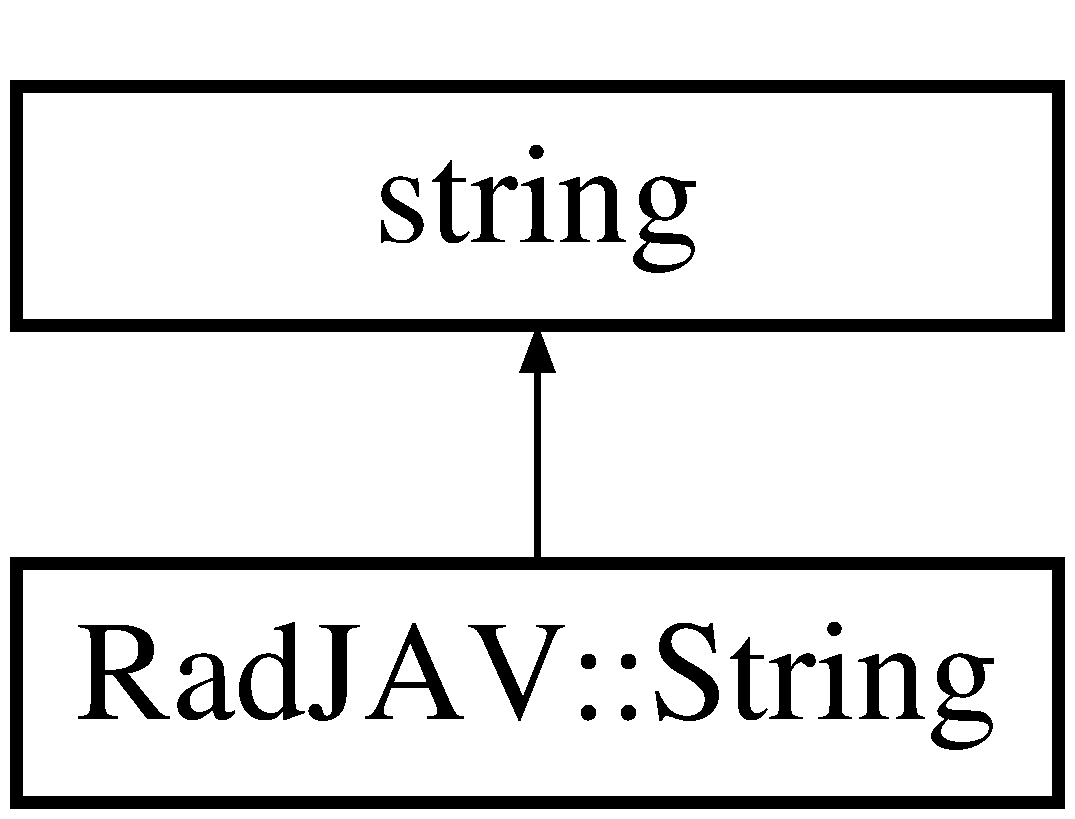
\includegraphics[height=2.000000cm]{class_rad_j_a_v_1_1_string}
\end{center}
\end{figure}
\subsection*{Public Member Functions}
\begin{DoxyCompactItemize}
\item 
\hyperlink{class_rad_j_a_v_1_1_string_a985090598133e2119dce64b79b176250}{String} ()
\item 
\hyperlink{class_rad_j_a_v_1_1_string_ab80c5e67a1b9c5bd24e75abfa0c8c77e}{String} (std\+::string str)
\item 
\hyperlink{class_rad_j_a_v_1_1_string_ac73be9671464715f5f461b242896ee0e}{String} (int value)
\item 
\hyperlink{class_rad_j_a_v_1_1_string_abdf12af39be1b08362731678b1edbf9c}{String} (const \hyperlink{class_rad_j_a_v_1_1_string}{String} \&str)
\item 
\hyperlink{class_rad_j_a_v_1_1_string_ab223546fa6dfdb4d6d5b80e846ab9642}{String} (const \hyperlink{class_rad_j_a_v_1_1_string}{String} \&str, size\+\_\+t pos, size\+\_\+t len=npos)
\item 
\hyperlink{class_rad_j_a_v_1_1_string_a56172a9c1c2e45232ed90cb4e79a9875}{String} (const char $\ast$str)
\item 
\hyperlink{class_rad_j_a_v_1_1_string_a71f9c004439cc655fe780c437d45c3d3}{String} (const char $\ast$str, size\+\_\+t len)
\item 
\hyperlink{class_rad_j_a_v_1_1_string_a37ca615c93d4853a3f6840fc3e29624e}{String} (size\+\_\+t len, char c)
\item 
{\footnotesize template$<$class Input\+Iterator $>$ }\\\hyperlink{class_rad_j_a_v_1_1_string_a028d4f2e378a4e60468e974cc7c1e81d}{String} (Input\+Iterator first, Input\+Iterator last)
\item 
std\+::vector$<$ \hyperlink{class_rad_j_a_v_1_1_string}{String} $>$ \hyperlink{class_rad_j_a_v_1_1_string_ad5550975cd1e484edf996381407a21e9}{split} (\hyperlink{class_rad_j_a_v_1_1_string}{String} delimiter)
\begin{DoxyCompactList}\small\item\em Split a string into an array of substrings seperated by a delimiter. \end{DoxyCompactList}\item 
std\+::vector$<$ \hyperlink{class_rad_j_a_v_1_1_string}{String} $>$ \hyperlink{class_rad_j_a_v_1_1_string_a7b5314ad977b2ab1c2d9452ed3103975}{split\+With\+Exceptions} (\hyperlink{class_rad_j_a_v_1_1_string}{String} delimiter, std\+::vector$<$ int $>$ exceptions\+Begin, std\+::vector$<$ int $>$ exceptions\+End)
\begin{DoxyCompactList}\small\item\em Split a string into an array of substrings seperated by a delimiter. \end{DoxyCompactList}\item 
\hyperlink{class_rad_j_a_v_1_1_string}{String} \hyperlink{class_rad_j_a_v_1_1_string_ab0343311b565d55201e97980f29c694d}{remove\+Whitespaces} ()
\begin{DoxyCompactList}\small\item\em Remove all whitespaces from a string. \end{DoxyCompactList}\item 
\hyperlink{class_rad_j_a_v_1_1_string}{String} \hyperlink{class_rad_j_a_v_1_1_string_a7b680e0853e2e221a7728b224ef3f2fe}{to\+Lower\+Case} ()
\begin{DoxyCompactList}\small\item\em Make a string lowercase. \end{DoxyCompactList}\item 
\hyperlink{class_rad_j_a_v_1_1_string}{String} \hyperlink{class_rad_j_a_v_1_1_string_a02e8c3b12ea21ce39d861050ee02627a}{to\+Upper\+Case} ()
\begin{DoxyCompactList}\small\item\em Make a string uppercase. \end{DoxyCompactList}\item 
bool \hyperlink{class_rad_j_a_v_1_1_string_a8f4fec14c1752e3edb811a6e6f9c99ce}{is\+Int} ()
\begin{DoxyCompactList}\small\item\em Check if a string is a valid integer. \end{DoxyCompactList}\item 
bool \hyperlink{class_rad_j_a_v_1_1_string_a51e463c671c993ce10184f68dac050d0}{is\+Double} ()
\begin{DoxyCompactList}\small\item\em Check if the string contains a double. \end{DoxyCompactList}\item 
bool \hyperlink{class_rad_j_a_v_1_1_string_a3fdf5f2aef734fffa2d23964668641be}{is\+Float} ()
\begin{DoxyCompactList}\small\item\em Check if the string contains a float. \end{DoxyCompactList}\item 
bool \hyperlink{class_rad_j_a_v_1_1_string_a07cb003b91b01e8dd78a7b534bdad243}{is\+Bool} (bool case\+Sensitive=false)
\begin{DoxyCompactList}\small\item\em Check if the string contains a boolean. \end{DoxyCompactList}\item 
\hyperlink{class_rad_j_a_v_1_1_string}{String} \hyperlink{class_rad_j_a_v_1_1_string_a8631dd8fc8ed789ab959315f7e73ddb4}{replace\+All} (\hyperlink{class_rad_j_a_v_1_1_string}{String} find, \hyperlink{class_rad_j_a_v_1_1_string}{String} replace\+With)
\begin{DoxyCompactList}\small\item\em Replace a string with another string. \end{DoxyCompactList}\end{DoxyCompactItemize}
\subsection*{Static Public Member Functions}
\begin{DoxyCompactItemize}
\item 
static \hyperlink{class_rad_j_a_v_1_1_string}{String} \hyperlink{class_rad_j_a_v_1_1_string_a6062497071348a2d203341c2f650085d}{from\+Int} (int i\+Integer)
\begin{DoxyCompactList}\small\item\em Convert an int into a string. \end{DoxyCompactList}\item 
static \hyperlink{class_rad_j_a_v_1_1_string}{String} \hyperlink{class_rad_j_a_v_1_1_string_a037777a57b94a36a6f55cc88d5a1b647}{from\+Long} (long value)
\begin{DoxyCompactList}\small\item\em Convert a long into a string. \end{DoxyCompactList}\item 
static \hyperlink{class_rad_j_a_v_1_1_string}{String} \hyperlink{class_rad_j_a_v_1_1_string_a8dafc3ee64efa449f35add3f598f0281}{from\+Unsigned\+Long} (unsigned long value)
\begin{DoxyCompactList}\small\item\em Convert an unsigned long into a string. \end{DoxyCompactList}\item 
static \hyperlink{class_rad_j_a_v_1_1_string}{String} \hyperlink{class_rad_j_a_v_1_1_string_a5501161ff54528c58720c23a30397519}{from\+Double} (double d\+Double)
\begin{DoxyCompactList}\small\item\em Convert a double into a string. \end{DoxyCompactList}\item 
static \hyperlink{class_rad_j_a_v_1_1_string}{String} \hyperlink{class_rad_j_a_v_1_1_string_a2dd011b85984bd4c4199b5fa07b24c6a}{from\+Float} (float f\+Float)
\begin{DoxyCompactList}\small\item\em Convert a float into a string. \end{DoxyCompactList}\item 
static \hyperlink{class_rad_j_a_v_1_1_string}{String} \hyperlink{class_rad_j_a_v_1_1_string_a169239aca74c7cb7fcee2f80cf868f62}{from\+Boolean} (bool b\+Bool)
\begin{DoxyCompactList}\small\item\em Convert a boolean into a string. \end{DoxyCompactList}\end{DoxyCompactItemize}


\subsection{Constructor \& Destructor Documentation}
\index{Rad\+J\+A\+V\+::\+String@{Rad\+J\+A\+V\+::\+String}!String@{String}}
\index{String@{String}!Rad\+J\+A\+V\+::\+String@{Rad\+J\+A\+V\+::\+String}}
\subsubsection[{\texorpdfstring{String()}{String()}}]{\setlength{\rightskip}{0pt plus 5cm}Rad\+J\+A\+V\+::\+String\+::\+String (
\begin{DoxyParamCaption}
{}
\end{DoxyParamCaption}
)\hspace{0.3cm}{\ttfamily [inline]}}\hypertarget{class_rad_j_a_v_1_1_string_a985090598133e2119dce64b79b176250}{}\label{class_rad_j_a_v_1_1_string_a985090598133e2119dce64b79b176250}
\index{Rad\+J\+A\+V\+::\+String@{Rad\+J\+A\+V\+::\+String}!String@{String}}
\index{String@{String}!Rad\+J\+A\+V\+::\+String@{Rad\+J\+A\+V\+::\+String}}
\subsubsection[{\texorpdfstring{String(std\+::string str)}{String(std::string str)}}]{\setlength{\rightskip}{0pt plus 5cm}Rad\+J\+A\+V\+::\+String\+::\+String (
\begin{DoxyParamCaption}
\item[{std\+::string}]{str}
\end{DoxyParamCaption}
)\hspace{0.3cm}{\ttfamily [inline]}}\hypertarget{class_rad_j_a_v_1_1_string_ab80c5e67a1b9c5bd24e75abfa0c8c77e}{}\label{class_rad_j_a_v_1_1_string_ab80c5e67a1b9c5bd24e75abfa0c8c77e}
\index{Rad\+J\+A\+V\+::\+String@{Rad\+J\+A\+V\+::\+String}!String@{String}}
\index{String@{String}!Rad\+J\+A\+V\+::\+String@{Rad\+J\+A\+V\+::\+String}}
\subsubsection[{\texorpdfstring{String(int value)}{String(int value)}}]{\setlength{\rightskip}{0pt plus 5cm}Rad\+J\+A\+V\+::\+String\+::\+String (
\begin{DoxyParamCaption}
\item[{int}]{value}
\end{DoxyParamCaption}
)\hspace{0.3cm}{\ttfamily [inline]}}\hypertarget{class_rad_j_a_v_1_1_string_ac73be9671464715f5f461b242896ee0e}{}\label{class_rad_j_a_v_1_1_string_ac73be9671464715f5f461b242896ee0e}
\index{Rad\+J\+A\+V\+::\+String@{Rad\+J\+A\+V\+::\+String}!String@{String}}
\index{String@{String}!Rad\+J\+A\+V\+::\+String@{Rad\+J\+A\+V\+::\+String}}
\subsubsection[{\texorpdfstring{String(const String \&str)}{String(const String &str)}}]{\setlength{\rightskip}{0pt plus 5cm}Rad\+J\+A\+V\+::\+String\+::\+String (
\begin{DoxyParamCaption}
\item[{const {\bf String} \&}]{str}
\end{DoxyParamCaption}
)\hspace{0.3cm}{\ttfamily [inline]}}\hypertarget{class_rad_j_a_v_1_1_string_abdf12af39be1b08362731678b1edbf9c}{}\label{class_rad_j_a_v_1_1_string_abdf12af39be1b08362731678b1edbf9c}
\index{Rad\+J\+A\+V\+::\+String@{Rad\+J\+A\+V\+::\+String}!String@{String}}
\index{String@{String}!Rad\+J\+A\+V\+::\+String@{Rad\+J\+A\+V\+::\+String}}
\subsubsection[{\texorpdfstring{String(const String \&str, size\+\_\+t pos, size\+\_\+t len=npos)}{String(const String &str, size_t pos, size_t len=npos)}}]{\setlength{\rightskip}{0pt plus 5cm}Rad\+J\+A\+V\+::\+String\+::\+String (
\begin{DoxyParamCaption}
\item[{const {\bf String} \&}]{str, }
\item[{size\+\_\+t}]{pos, }
\item[{size\+\_\+t}]{len = {\ttfamily npos}}
\end{DoxyParamCaption}
)\hspace{0.3cm}{\ttfamily [inline]}}\hypertarget{class_rad_j_a_v_1_1_string_ab223546fa6dfdb4d6d5b80e846ab9642}{}\label{class_rad_j_a_v_1_1_string_ab223546fa6dfdb4d6d5b80e846ab9642}
\index{Rad\+J\+A\+V\+::\+String@{Rad\+J\+A\+V\+::\+String}!String@{String}}
\index{String@{String}!Rad\+J\+A\+V\+::\+String@{Rad\+J\+A\+V\+::\+String}}
\subsubsection[{\texorpdfstring{String(const char $\ast$str)}{String(const char *str)}}]{\setlength{\rightskip}{0pt plus 5cm}Rad\+J\+A\+V\+::\+String\+::\+String (
\begin{DoxyParamCaption}
\item[{const char $\ast$}]{str}
\end{DoxyParamCaption}
)\hspace{0.3cm}{\ttfamily [inline]}}\hypertarget{class_rad_j_a_v_1_1_string_a56172a9c1c2e45232ed90cb4e79a9875}{}\label{class_rad_j_a_v_1_1_string_a56172a9c1c2e45232ed90cb4e79a9875}
\index{Rad\+J\+A\+V\+::\+String@{Rad\+J\+A\+V\+::\+String}!String@{String}}
\index{String@{String}!Rad\+J\+A\+V\+::\+String@{Rad\+J\+A\+V\+::\+String}}
\subsubsection[{\texorpdfstring{String(const char $\ast$str, size\+\_\+t len)}{String(const char *str, size_t len)}}]{\setlength{\rightskip}{0pt plus 5cm}Rad\+J\+A\+V\+::\+String\+::\+String (
\begin{DoxyParamCaption}
\item[{const char $\ast$}]{str, }
\item[{size\+\_\+t}]{len}
\end{DoxyParamCaption}
)\hspace{0.3cm}{\ttfamily [inline]}}\hypertarget{class_rad_j_a_v_1_1_string_a71f9c004439cc655fe780c437d45c3d3}{}\label{class_rad_j_a_v_1_1_string_a71f9c004439cc655fe780c437d45c3d3}
\index{Rad\+J\+A\+V\+::\+String@{Rad\+J\+A\+V\+::\+String}!String@{String}}
\index{String@{String}!Rad\+J\+A\+V\+::\+String@{Rad\+J\+A\+V\+::\+String}}
\subsubsection[{\texorpdfstring{String(size\+\_\+t len, char c)}{String(size_t len, char c)}}]{\setlength{\rightskip}{0pt plus 5cm}Rad\+J\+A\+V\+::\+String\+::\+String (
\begin{DoxyParamCaption}
\item[{size\+\_\+t}]{len, }
\item[{char}]{c}
\end{DoxyParamCaption}
)\hspace{0.3cm}{\ttfamily [inline]}}\hypertarget{class_rad_j_a_v_1_1_string_a37ca615c93d4853a3f6840fc3e29624e}{}\label{class_rad_j_a_v_1_1_string_a37ca615c93d4853a3f6840fc3e29624e}
\index{Rad\+J\+A\+V\+::\+String@{Rad\+J\+A\+V\+::\+String}!String@{String}}
\index{String@{String}!Rad\+J\+A\+V\+::\+String@{Rad\+J\+A\+V\+::\+String}}
\subsubsection[{\texorpdfstring{String(\+Input\+Iterator first, Input\+Iterator last)}{String(InputIterator first, InputIterator last)}}]{\setlength{\rightskip}{0pt plus 5cm}template$<$class Input\+Iterator $>$ Rad\+J\+A\+V\+::\+String\+::\+String (
\begin{DoxyParamCaption}
\item[{Input\+Iterator}]{first, }
\item[{Input\+Iterator}]{last}
\end{DoxyParamCaption}
)\hspace{0.3cm}{\ttfamily [inline]}}\hypertarget{class_rad_j_a_v_1_1_string_a028d4f2e378a4e60468e974cc7c1e81d}{}\label{class_rad_j_a_v_1_1_string_a028d4f2e378a4e60468e974cc7c1e81d}


\subsection{Member Function Documentation}
\index{Rad\+J\+A\+V\+::\+String@{Rad\+J\+A\+V\+::\+String}!from\+Boolean@{from\+Boolean}}
\index{from\+Boolean@{from\+Boolean}!Rad\+J\+A\+V\+::\+String@{Rad\+J\+A\+V\+::\+String}}
\subsubsection[{\texorpdfstring{from\+Boolean(bool b\+Bool)}{fromBoolean(bool bBool)}}]{\setlength{\rightskip}{0pt plus 5cm}{\bf String} Rad\+J\+A\+V\+::\+String\+::from\+Boolean (
\begin{DoxyParamCaption}
\item[{bool}]{b\+Bool}
\end{DoxyParamCaption}
)\hspace{0.3cm}{\ttfamily [static]}}\hypertarget{class_rad_j_a_v_1_1_string_a169239aca74c7cb7fcee2f80cf868f62}{}\label{class_rad_j_a_v_1_1_string_a169239aca74c7cb7fcee2f80cf868f62}


Convert a boolean into a string. 

\index{Rad\+J\+A\+V\+::\+String@{Rad\+J\+A\+V\+::\+String}!from\+Double@{from\+Double}}
\index{from\+Double@{from\+Double}!Rad\+J\+A\+V\+::\+String@{Rad\+J\+A\+V\+::\+String}}
\subsubsection[{\texorpdfstring{from\+Double(double d\+Double)}{fromDouble(double dDouble)}}]{\setlength{\rightskip}{0pt plus 5cm}{\bf String} Rad\+J\+A\+V\+::\+String\+::from\+Double (
\begin{DoxyParamCaption}
\item[{double}]{d\+Double}
\end{DoxyParamCaption}
)\hspace{0.3cm}{\ttfamily [static]}}\hypertarget{class_rad_j_a_v_1_1_string_a5501161ff54528c58720c23a30397519}{}\label{class_rad_j_a_v_1_1_string_a5501161ff54528c58720c23a30397519}


Convert a double into a string. 

\index{Rad\+J\+A\+V\+::\+String@{Rad\+J\+A\+V\+::\+String}!from\+Float@{from\+Float}}
\index{from\+Float@{from\+Float}!Rad\+J\+A\+V\+::\+String@{Rad\+J\+A\+V\+::\+String}}
\subsubsection[{\texorpdfstring{from\+Float(float f\+Float)}{fromFloat(float fFloat)}}]{\setlength{\rightskip}{0pt plus 5cm}{\bf String} Rad\+J\+A\+V\+::\+String\+::from\+Float (
\begin{DoxyParamCaption}
\item[{float}]{f\+Float}
\end{DoxyParamCaption}
)\hspace{0.3cm}{\ttfamily [static]}}\hypertarget{class_rad_j_a_v_1_1_string_a2dd011b85984bd4c4199b5fa07b24c6a}{}\label{class_rad_j_a_v_1_1_string_a2dd011b85984bd4c4199b5fa07b24c6a}


Convert a float into a string. 

\index{Rad\+J\+A\+V\+::\+String@{Rad\+J\+A\+V\+::\+String}!from\+Int@{from\+Int}}
\index{from\+Int@{from\+Int}!Rad\+J\+A\+V\+::\+String@{Rad\+J\+A\+V\+::\+String}}
\subsubsection[{\texorpdfstring{from\+Int(int i\+Integer)}{fromInt(int iInteger)}}]{\setlength{\rightskip}{0pt plus 5cm}{\bf String} Rad\+J\+A\+V\+::\+String\+::from\+Int (
\begin{DoxyParamCaption}
\item[{int}]{i\+Integer}
\end{DoxyParamCaption}
)\hspace{0.3cm}{\ttfamily [static]}}\hypertarget{class_rad_j_a_v_1_1_string_a6062497071348a2d203341c2f650085d}{}\label{class_rad_j_a_v_1_1_string_a6062497071348a2d203341c2f650085d}


Convert an int into a string. 

\index{Rad\+J\+A\+V\+::\+String@{Rad\+J\+A\+V\+::\+String}!from\+Long@{from\+Long}}
\index{from\+Long@{from\+Long}!Rad\+J\+A\+V\+::\+String@{Rad\+J\+A\+V\+::\+String}}
\subsubsection[{\texorpdfstring{from\+Long(long value)}{fromLong(long value)}}]{\setlength{\rightskip}{0pt plus 5cm}{\bf String} Rad\+J\+A\+V\+::\+String\+::from\+Long (
\begin{DoxyParamCaption}
\item[{long}]{value}
\end{DoxyParamCaption}
)\hspace{0.3cm}{\ttfamily [static]}}\hypertarget{class_rad_j_a_v_1_1_string_a037777a57b94a36a6f55cc88d5a1b647}{}\label{class_rad_j_a_v_1_1_string_a037777a57b94a36a6f55cc88d5a1b647}


Convert a long into a string. 

\index{Rad\+J\+A\+V\+::\+String@{Rad\+J\+A\+V\+::\+String}!from\+Unsigned\+Long@{from\+Unsigned\+Long}}
\index{from\+Unsigned\+Long@{from\+Unsigned\+Long}!Rad\+J\+A\+V\+::\+String@{Rad\+J\+A\+V\+::\+String}}
\subsubsection[{\texorpdfstring{from\+Unsigned\+Long(unsigned long value)}{fromUnsignedLong(unsigned long value)}}]{\setlength{\rightskip}{0pt plus 5cm}{\bf String} Rad\+J\+A\+V\+::\+String\+::from\+Unsigned\+Long (
\begin{DoxyParamCaption}
\item[{unsigned long}]{value}
\end{DoxyParamCaption}
)\hspace{0.3cm}{\ttfamily [static]}}\hypertarget{class_rad_j_a_v_1_1_string_a8dafc3ee64efa449f35add3f598f0281}{}\label{class_rad_j_a_v_1_1_string_a8dafc3ee64efa449f35add3f598f0281}


Convert an unsigned long into a string. 

\index{Rad\+J\+A\+V\+::\+String@{Rad\+J\+A\+V\+::\+String}!is\+Bool@{is\+Bool}}
\index{is\+Bool@{is\+Bool}!Rad\+J\+A\+V\+::\+String@{Rad\+J\+A\+V\+::\+String}}
\subsubsection[{\texorpdfstring{is\+Bool(bool case\+Sensitive=false)}{isBool(bool caseSensitive=false)}}]{\setlength{\rightskip}{0pt plus 5cm}bool Rad\+J\+A\+V\+::\+String\+::is\+Bool (
\begin{DoxyParamCaption}
\item[{bool}]{case\+Sensitive = {\ttfamily false}}
\end{DoxyParamCaption}
)}\hypertarget{class_rad_j_a_v_1_1_string_a07cb003b91b01e8dd78a7b534bdad243}{}\label{class_rad_j_a_v_1_1_string_a07cb003b91b01e8dd78a7b534bdad243}


Check if the string contains a boolean. 

\index{Rad\+J\+A\+V\+::\+String@{Rad\+J\+A\+V\+::\+String}!is\+Double@{is\+Double}}
\index{is\+Double@{is\+Double}!Rad\+J\+A\+V\+::\+String@{Rad\+J\+A\+V\+::\+String}}
\subsubsection[{\texorpdfstring{is\+Double()}{isDouble()}}]{\setlength{\rightskip}{0pt plus 5cm}bool Rad\+J\+A\+V\+::\+String\+::is\+Double (
\begin{DoxyParamCaption}
{}
\end{DoxyParamCaption}
)}\hypertarget{class_rad_j_a_v_1_1_string_a51e463c671c993ce10184f68dac050d0}{}\label{class_rad_j_a_v_1_1_string_a51e463c671c993ce10184f68dac050d0}


Check if the string contains a double. 

\index{Rad\+J\+A\+V\+::\+String@{Rad\+J\+A\+V\+::\+String}!is\+Float@{is\+Float}}
\index{is\+Float@{is\+Float}!Rad\+J\+A\+V\+::\+String@{Rad\+J\+A\+V\+::\+String}}
\subsubsection[{\texorpdfstring{is\+Float()}{isFloat()}}]{\setlength{\rightskip}{0pt plus 5cm}bool Rad\+J\+A\+V\+::\+String\+::is\+Float (
\begin{DoxyParamCaption}
{}
\end{DoxyParamCaption}
)}\hypertarget{class_rad_j_a_v_1_1_string_a3fdf5f2aef734fffa2d23964668641be}{}\label{class_rad_j_a_v_1_1_string_a3fdf5f2aef734fffa2d23964668641be}


Check if the string contains a float. 

\index{Rad\+J\+A\+V\+::\+String@{Rad\+J\+A\+V\+::\+String}!is\+Int@{is\+Int}}
\index{is\+Int@{is\+Int}!Rad\+J\+A\+V\+::\+String@{Rad\+J\+A\+V\+::\+String}}
\subsubsection[{\texorpdfstring{is\+Int()}{isInt()}}]{\setlength{\rightskip}{0pt plus 5cm}bool Rad\+J\+A\+V\+::\+String\+::is\+Int (
\begin{DoxyParamCaption}
{}
\end{DoxyParamCaption}
)}\hypertarget{class_rad_j_a_v_1_1_string_a8f4fec14c1752e3edb811a6e6f9c99ce}{}\label{class_rad_j_a_v_1_1_string_a8f4fec14c1752e3edb811a6e6f9c99ce}


Check if a string is a valid integer. 

\index{Rad\+J\+A\+V\+::\+String@{Rad\+J\+A\+V\+::\+String}!remove\+Whitespaces@{remove\+Whitespaces}}
\index{remove\+Whitespaces@{remove\+Whitespaces}!Rad\+J\+A\+V\+::\+String@{Rad\+J\+A\+V\+::\+String}}
\subsubsection[{\texorpdfstring{remove\+Whitespaces()}{removeWhitespaces()}}]{\setlength{\rightskip}{0pt plus 5cm}{\bf String} Rad\+J\+A\+V\+::\+String\+::remove\+Whitespaces (
\begin{DoxyParamCaption}
{}
\end{DoxyParamCaption}
)}\hypertarget{class_rad_j_a_v_1_1_string_ab0343311b565d55201e97980f29c694d}{}\label{class_rad_j_a_v_1_1_string_ab0343311b565d55201e97980f29c694d}


Remove all whitespaces from a string. 

\index{Rad\+J\+A\+V\+::\+String@{Rad\+J\+A\+V\+::\+String}!replace\+All@{replace\+All}}
\index{replace\+All@{replace\+All}!Rad\+J\+A\+V\+::\+String@{Rad\+J\+A\+V\+::\+String}}
\subsubsection[{\texorpdfstring{replace\+All(\+String find, String replace\+With)}{replaceAll(String find, String replaceWith)}}]{\setlength{\rightskip}{0pt plus 5cm}{\bf String} Rad\+J\+A\+V\+::\+String\+::replace\+All (
\begin{DoxyParamCaption}
\item[{{\bf String}}]{find, }
\item[{{\bf String}}]{replace\+With}
\end{DoxyParamCaption}
)}\hypertarget{class_rad_j_a_v_1_1_string_a8631dd8fc8ed789ab959315f7e73ddb4}{}\label{class_rad_j_a_v_1_1_string_a8631dd8fc8ed789ab959315f7e73ddb4}


Replace a string with another string. 

\index{Rad\+J\+A\+V\+::\+String@{Rad\+J\+A\+V\+::\+String}!split@{split}}
\index{split@{split}!Rad\+J\+A\+V\+::\+String@{Rad\+J\+A\+V\+::\+String}}
\subsubsection[{\texorpdfstring{split(\+String delimiter)}{split(String delimiter)}}]{\setlength{\rightskip}{0pt plus 5cm}std\+::vector$<$ {\bf String} $>$ Rad\+J\+A\+V\+::\+String\+::split (
\begin{DoxyParamCaption}
\item[{{\bf String}}]{delimiter}
\end{DoxyParamCaption}
)}\hypertarget{class_rad_j_a_v_1_1_string_ad5550975cd1e484edf996381407a21e9}{}\label{class_rad_j_a_v_1_1_string_ad5550975cd1e484edf996381407a21e9}


Split a string into an array of substrings seperated by a delimiter. 

\index{Rad\+J\+A\+V\+::\+String@{Rad\+J\+A\+V\+::\+String}!split\+With\+Exceptions@{split\+With\+Exceptions}}
\index{split\+With\+Exceptions@{split\+With\+Exceptions}!Rad\+J\+A\+V\+::\+String@{Rad\+J\+A\+V\+::\+String}}
\subsubsection[{\texorpdfstring{split\+With\+Exceptions(\+String delimiter, std\+::vector$<$ int $>$ exceptions\+Begin, std\+::vector$<$ int $>$ exceptions\+End)}{splitWithExceptions(String delimiter, std::vector< int > exceptionsBegin, std::vector< int > exceptionsEnd)}}]{\setlength{\rightskip}{0pt plus 5cm}std\+::vector$<$ {\bf String} $>$ Rad\+J\+A\+V\+::\+String\+::split\+With\+Exceptions (
\begin{DoxyParamCaption}
\item[{{\bf String}}]{delimiter, }
\item[{std\+::vector$<$ int $>$}]{exceptions\+Begin, }
\item[{std\+::vector$<$ int $>$}]{exceptions\+End}
\end{DoxyParamCaption}
)}\hypertarget{class_rad_j_a_v_1_1_string_a7b5314ad977b2ab1c2d9452ed3103975}{}\label{class_rad_j_a_v_1_1_string_a7b5314ad977b2ab1c2d9452ed3103975}


Split a string into an array of substrings seperated by a delimiter. 

\index{Rad\+J\+A\+V\+::\+String@{Rad\+J\+A\+V\+::\+String}!to\+Lower\+Case@{to\+Lower\+Case}}
\index{to\+Lower\+Case@{to\+Lower\+Case}!Rad\+J\+A\+V\+::\+String@{Rad\+J\+A\+V\+::\+String}}
\subsubsection[{\texorpdfstring{to\+Lower\+Case()}{toLowerCase()}}]{\setlength{\rightskip}{0pt plus 5cm}{\bf String} Rad\+J\+A\+V\+::\+String\+::to\+Lower\+Case (
\begin{DoxyParamCaption}
{}
\end{DoxyParamCaption}
)}\hypertarget{class_rad_j_a_v_1_1_string_a7b680e0853e2e221a7728b224ef3f2fe}{}\label{class_rad_j_a_v_1_1_string_a7b680e0853e2e221a7728b224ef3f2fe}


Make a string lowercase. 

\index{Rad\+J\+A\+V\+::\+String@{Rad\+J\+A\+V\+::\+String}!to\+Upper\+Case@{to\+Upper\+Case}}
\index{to\+Upper\+Case@{to\+Upper\+Case}!Rad\+J\+A\+V\+::\+String@{Rad\+J\+A\+V\+::\+String}}
\subsubsection[{\texorpdfstring{to\+Upper\+Case()}{toUpperCase()}}]{\setlength{\rightskip}{0pt plus 5cm}{\bf String} Rad\+J\+A\+V\+::\+String\+::to\+Upper\+Case (
\begin{DoxyParamCaption}
{}
\end{DoxyParamCaption}
)}\hypertarget{class_rad_j_a_v_1_1_string_a02e8c3b12ea21ce39d861050ee02627a}{}\label{class_rad_j_a_v_1_1_string_a02e8c3b12ea21ce39d861050ee02627a}


Make a string uppercase. 



The documentation for this class was generated from the following files\+:\begin{DoxyCompactItemize}
\item 
include/\+Rad\+Jav/\hyperlink{_rad_jav_string_8h}{Rad\+Jav\+String.\+h}\item 
src/\+Rad\+Jav/\hyperlink{_rad_jav_string_8cpp}{Rad\+Jav\+String.\+cpp}\end{DoxyCompactItemize}

\hypertarget{class_rad_j_a_v_1_1_networking_1_1_t_c_p_connection}{}\section{Rad\+J\+AV\+:\+:Networking\+:\+:T\+C\+P\+Connection Class Reference}
\label{class_rad_j_a_v_1_1_networking_1_1_t_c_p_connection}\index{Rad\+J\+A\+V\+::\+Networking\+::\+T\+C\+P\+Connection@{Rad\+J\+A\+V\+::\+Networking\+::\+T\+C\+P\+Connection}}


Represents a T\+CP connection.  




{\ttfamily \#include $<$Rad\+Jav\+Networking.\+h$>$}

\subsection*{Public Member Functions}
\begin{DoxyCompactItemize}
\item 
\hyperlink{class_rad_j_a_v_1_1_networking_1_1_t_c_p_connection_a0fab77382e716af1b1c425f9d5102fc2}{T\+C\+P\+Connection} (\hyperlink{class_rad_j_a_v_1_1_networking_1_1_i_pv4}{I\+Pv4} ip)
\item 
\hyperlink{class_rad_j_a_v_1_1_networking_1_1_t_c_p_connection_ae181a2c7528971d495bcefaf437729a5}{T\+C\+P\+Connection} (\hyperlink{class_rad_j_a_v_1_1_networking_1_1_i_pv6}{I\+Pv6} ip)
\item 
int \hyperlink{class_rad_j_a_v_1_1_networking_1_1_t_c_p_connection_ab3753143cc5c17927826650189c4760a}{get\+Connection\+Type} ()
\begin{DoxyCompactList}\small\item\em Get the type of T\+CP connection that\textquotesingle{}s used. \end{DoxyCompactList}\item 
\hyperlink{class_rad_j_a_v_1_1_networking_1_1_i_pv4}{I\+Pv4} \hyperlink{class_rad_j_a_v_1_1_networking_1_1_t_c_p_connection_afe488c0f221c460086b7b8e11e9c9163}{get\+I\+Pv4} ()
\begin{DoxyCompactList}\small\item\em Get the T\+C\+Pv4 address being used. \end{DoxyCompactList}\item 
\hyperlink{class_rad_j_a_v_1_1_networking_1_1_i_pv6}{I\+Pv6} \hyperlink{class_rad_j_a_v_1_1_networking_1_1_t_c_p_connection_a49cbcbef604c97fb4381d7e2982e355e}{get\+I\+Pv6} ()
\begin{DoxyCompactList}\small\item\em Get the T\+C\+Pv6 address being used. \end{DoxyCompactList}\item 
unsigned int \hyperlink{class_rad_j_a_v_1_1_networking_1_1_t_c_p_connection_a79c163ef7d1d0d1ed4179e9dab39cb2f}{get\+Id} ()
\begin{DoxyCompactList}\small\item\em Get connection id. \end{DoxyCompactList}\item 
\hyperlink{class_rad_j_a_v_1_1_string}{String} \hyperlink{class_rad_j_a_v_1_1_networking_1_1_t_c_p_connection_a380090258c8b5aa6c2f9b0b7c0bec24c}{get\+IP} ()
\begin{DoxyCompactList}\small\item\em Get the IP as a string. \end{DoxyCompactList}\end{DoxyCompactItemize}
\subsection*{Protected Member Functions}
\begin{DoxyCompactItemize}
\item 
unsigned int \hyperlink{class_rad_j_a_v_1_1_networking_1_1_t_c_p_connection_a13ed8b099258871e241e52b14d568073}{get\+New\+Id} ()
\end{DoxyCompactItemize}
\subsection*{Protected Attributes}
\begin{DoxyCompactItemize}
\item 
unsigned int \hyperlink{class_rad_j_a_v_1_1_networking_1_1_t_c_p_connection_ac513874994cf8b03127b001e5a7094bd}{id}
\item 
int \hyperlink{class_rad_j_a_v_1_1_networking_1_1_t_c_p_connection_ae24db0c9dac2a7ae3c41afd17ff65d80}{connection\+Type}
\item 
\hyperlink{class_rad_j_a_v_1_1_networking_1_1_i_pv4}{I\+Pv4} \hyperlink{class_rad_j_a_v_1_1_networking_1_1_t_c_p_connection_a2dc53527dc30118419d87d2934d032ae}{ipv4}
\item 
\hyperlink{class_rad_j_a_v_1_1_networking_1_1_i_pv6}{I\+Pv6} \hyperlink{class_rad_j_a_v_1_1_networking_1_1_t_c_p_connection_a3ddda74035ec41a86c9431c084cd0097}{ipv6}
\end{DoxyCompactItemize}
\subsection*{Static Protected Attributes}
\begin{DoxyCompactItemize}
\item 
static int \hyperlink{class_rad_j_a_v_1_1_networking_1_1_t_c_p_connection_a342f7c52a3e4c2567b8263f68109ffcb}{num\+Connections} = 0
\end{DoxyCompactItemize}


\subsection{Detailed Description}
Represents a T\+CP connection. 

\subsection{Constructor \& Destructor Documentation}
\index{Rad\+J\+A\+V\+::\+Networking\+::\+T\+C\+P\+Connection@{Rad\+J\+A\+V\+::\+Networking\+::\+T\+C\+P\+Connection}!T\+C\+P\+Connection@{T\+C\+P\+Connection}}
\index{T\+C\+P\+Connection@{T\+C\+P\+Connection}!Rad\+J\+A\+V\+::\+Networking\+::\+T\+C\+P\+Connection@{Rad\+J\+A\+V\+::\+Networking\+::\+T\+C\+P\+Connection}}
\subsubsection[{\texorpdfstring{T\+C\+P\+Connection(\+I\+Pv4 ip)}{TCPConnection(IPv4 ip)}}]{\setlength{\rightskip}{0pt plus 5cm}Rad\+J\+A\+V\+::\+Networking\+::\+T\+C\+P\+Connection\+::\+T\+C\+P\+Connection (
\begin{DoxyParamCaption}
\item[{{\bf I\+Pv4}}]{ip}
\end{DoxyParamCaption}
)\hspace{0.3cm}{\ttfamily [inline]}}\hypertarget{class_rad_j_a_v_1_1_networking_1_1_t_c_p_connection_a0fab77382e716af1b1c425f9d5102fc2}{}\label{class_rad_j_a_v_1_1_networking_1_1_t_c_p_connection_a0fab77382e716af1b1c425f9d5102fc2}
\index{Rad\+J\+A\+V\+::\+Networking\+::\+T\+C\+P\+Connection@{Rad\+J\+A\+V\+::\+Networking\+::\+T\+C\+P\+Connection}!T\+C\+P\+Connection@{T\+C\+P\+Connection}}
\index{T\+C\+P\+Connection@{T\+C\+P\+Connection}!Rad\+J\+A\+V\+::\+Networking\+::\+T\+C\+P\+Connection@{Rad\+J\+A\+V\+::\+Networking\+::\+T\+C\+P\+Connection}}
\subsubsection[{\texorpdfstring{T\+C\+P\+Connection(\+I\+Pv6 ip)}{TCPConnection(IPv6 ip)}}]{\setlength{\rightskip}{0pt plus 5cm}Rad\+J\+A\+V\+::\+Networking\+::\+T\+C\+P\+Connection\+::\+T\+C\+P\+Connection (
\begin{DoxyParamCaption}
\item[{{\bf I\+Pv6}}]{ip}
\end{DoxyParamCaption}
)\hspace{0.3cm}{\ttfamily [inline]}}\hypertarget{class_rad_j_a_v_1_1_networking_1_1_t_c_p_connection_ae181a2c7528971d495bcefaf437729a5}{}\label{class_rad_j_a_v_1_1_networking_1_1_t_c_p_connection_ae181a2c7528971d495bcefaf437729a5}


\subsection{Member Function Documentation}
\index{Rad\+J\+A\+V\+::\+Networking\+::\+T\+C\+P\+Connection@{Rad\+J\+A\+V\+::\+Networking\+::\+T\+C\+P\+Connection}!get\+Connection\+Type@{get\+Connection\+Type}}
\index{get\+Connection\+Type@{get\+Connection\+Type}!Rad\+J\+A\+V\+::\+Networking\+::\+T\+C\+P\+Connection@{Rad\+J\+A\+V\+::\+Networking\+::\+T\+C\+P\+Connection}}
\subsubsection[{\texorpdfstring{get\+Connection\+Type()}{getConnectionType()}}]{\setlength{\rightskip}{0pt plus 5cm}int Rad\+J\+A\+V\+::\+Networking\+::\+T\+C\+P\+Connection\+::get\+Connection\+Type (
\begin{DoxyParamCaption}
{}
\end{DoxyParamCaption}
)\hspace{0.3cm}{\ttfamily [inline]}}\hypertarget{class_rad_j_a_v_1_1_networking_1_1_t_c_p_connection_ab3753143cc5c17927826650189c4760a}{}\label{class_rad_j_a_v_1_1_networking_1_1_t_c_p_connection_ab3753143cc5c17927826650189c4760a}


Get the type of T\+CP connection that\textquotesingle{}s used. 

\index{Rad\+J\+A\+V\+::\+Networking\+::\+T\+C\+P\+Connection@{Rad\+J\+A\+V\+::\+Networking\+::\+T\+C\+P\+Connection}!get\+Id@{get\+Id}}
\index{get\+Id@{get\+Id}!Rad\+J\+A\+V\+::\+Networking\+::\+T\+C\+P\+Connection@{Rad\+J\+A\+V\+::\+Networking\+::\+T\+C\+P\+Connection}}
\subsubsection[{\texorpdfstring{get\+Id()}{getId()}}]{\setlength{\rightskip}{0pt plus 5cm}unsigned int Rad\+J\+A\+V\+::\+Networking\+::\+T\+C\+P\+Connection\+::get\+Id (
\begin{DoxyParamCaption}
{}
\end{DoxyParamCaption}
)\hspace{0.3cm}{\ttfamily [inline]}}\hypertarget{class_rad_j_a_v_1_1_networking_1_1_t_c_p_connection_a79c163ef7d1d0d1ed4179e9dab39cb2f}{}\label{class_rad_j_a_v_1_1_networking_1_1_t_c_p_connection_a79c163ef7d1d0d1ed4179e9dab39cb2f}


Get connection id. 

\index{Rad\+J\+A\+V\+::\+Networking\+::\+T\+C\+P\+Connection@{Rad\+J\+A\+V\+::\+Networking\+::\+T\+C\+P\+Connection}!get\+IP@{get\+IP}}
\index{get\+IP@{get\+IP}!Rad\+J\+A\+V\+::\+Networking\+::\+T\+C\+P\+Connection@{Rad\+J\+A\+V\+::\+Networking\+::\+T\+C\+P\+Connection}}
\subsubsection[{\texorpdfstring{get\+I\+P()}{getIP()}}]{\setlength{\rightskip}{0pt plus 5cm}{\bf String} Rad\+J\+A\+V\+::\+Networking\+::\+T\+C\+P\+Connection\+::get\+IP (
\begin{DoxyParamCaption}
{}
\end{DoxyParamCaption}
)\hspace{0.3cm}{\ttfamily [inline]}}\hypertarget{class_rad_j_a_v_1_1_networking_1_1_t_c_p_connection_a380090258c8b5aa6c2f9b0b7c0bec24c}{}\label{class_rad_j_a_v_1_1_networking_1_1_t_c_p_connection_a380090258c8b5aa6c2f9b0b7c0bec24c}


Get the IP as a string. 

\index{Rad\+J\+A\+V\+::\+Networking\+::\+T\+C\+P\+Connection@{Rad\+J\+A\+V\+::\+Networking\+::\+T\+C\+P\+Connection}!get\+I\+Pv4@{get\+I\+Pv4}}
\index{get\+I\+Pv4@{get\+I\+Pv4}!Rad\+J\+A\+V\+::\+Networking\+::\+T\+C\+P\+Connection@{Rad\+J\+A\+V\+::\+Networking\+::\+T\+C\+P\+Connection}}
\subsubsection[{\texorpdfstring{get\+I\+Pv4()}{getIPv4()}}]{\setlength{\rightskip}{0pt plus 5cm}{\bf I\+Pv4} Rad\+J\+A\+V\+::\+Networking\+::\+T\+C\+P\+Connection\+::get\+I\+Pv4 (
\begin{DoxyParamCaption}
{}
\end{DoxyParamCaption}
)\hspace{0.3cm}{\ttfamily [inline]}}\hypertarget{class_rad_j_a_v_1_1_networking_1_1_t_c_p_connection_afe488c0f221c460086b7b8e11e9c9163}{}\label{class_rad_j_a_v_1_1_networking_1_1_t_c_p_connection_afe488c0f221c460086b7b8e11e9c9163}


Get the T\+C\+Pv4 address being used. 

\index{Rad\+J\+A\+V\+::\+Networking\+::\+T\+C\+P\+Connection@{Rad\+J\+A\+V\+::\+Networking\+::\+T\+C\+P\+Connection}!get\+I\+Pv6@{get\+I\+Pv6}}
\index{get\+I\+Pv6@{get\+I\+Pv6}!Rad\+J\+A\+V\+::\+Networking\+::\+T\+C\+P\+Connection@{Rad\+J\+A\+V\+::\+Networking\+::\+T\+C\+P\+Connection}}
\subsubsection[{\texorpdfstring{get\+I\+Pv6()}{getIPv6()}}]{\setlength{\rightskip}{0pt plus 5cm}{\bf I\+Pv6} Rad\+J\+A\+V\+::\+Networking\+::\+T\+C\+P\+Connection\+::get\+I\+Pv6 (
\begin{DoxyParamCaption}
{}
\end{DoxyParamCaption}
)\hspace{0.3cm}{\ttfamily [inline]}}\hypertarget{class_rad_j_a_v_1_1_networking_1_1_t_c_p_connection_a49cbcbef604c97fb4381d7e2982e355e}{}\label{class_rad_j_a_v_1_1_networking_1_1_t_c_p_connection_a49cbcbef604c97fb4381d7e2982e355e}


Get the T\+C\+Pv6 address being used. 

\index{Rad\+J\+A\+V\+::\+Networking\+::\+T\+C\+P\+Connection@{Rad\+J\+A\+V\+::\+Networking\+::\+T\+C\+P\+Connection}!get\+New\+Id@{get\+New\+Id}}
\index{get\+New\+Id@{get\+New\+Id}!Rad\+J\+A\+V\+::\+Networking\+::\+T\+C\+P\+Connection@{Rad\+J\+A\+V\+::\+Networking\+::\+T\+C\+P\+Connection}}
\subsubsection[{\texorpdfstring{get\+New\+Id()}{getNewId()}}]{\setlength{\rightskip}{0pt plus 5cm}unsigned int Rad\+J\+A\+V\+::\+Networking\+::\+T\+C\+P\+Connection\+::get\+New\+Id (
\begin{DoxyParamCaption}
{}
\end{DoxyParamCaption}
)\hspace{0.3cm}{\ttfamily [inline]}, {\ttfamily [protected]}}\hypertarget{class_rad_j_a_v_1_1_networking_1_1_t_c_p_connection_a13ed8b099258871e241e52b14d568073}{}\label{class_rad_j_a_v_1_1_networking_1_1_t_c_p_connection_a13ed8b099258871e241e52b14d568073}


\subsection{Member Data Documentation}
\index{Rad\+J\+A\+V\+::\+Networking\+::\+T\+C\+P\+Connection@{Rad\+J\+A\+V\+::\+Networking\+::\+T\+C\+P\+Connection}!connection\+Type@{connection\+Type}}
\index{connection\+Type@{connection\+Type}!Rad\+J\+A\+V\+::\+Networking\+::\+T\+C\+P\+Connection@{Rad\+J\+A\+V\+::\+Networking\+::\+T\+C\+P\+Connection}}
\subsubsection[{\texorpdfstring{connection\+Type}{connectionType}}]{\setlength{\rightskip}{0pt plus 5cm}int Rad\+J\+A\+V\+::\+Networking\+::\+T\+C\+P\+Connection\+::connection\+Type\hspace{0.3cm}{\ttfamily [protected]}}\hypertarget{class_rad_j_a_v_1_1_networking_1_1_t_c_p_connection_ae24db0c9dac2a7ae3c41afd17ff65d80}{}\label{class_rad_j_a_v_1_1_networking_1_1_t_c_p_connection_ae24db0c9dac2a7ae3c41afd17ff65d80}
\index{Rad\+J\+A\+V\+::\+Networking\+::\+T\+C\+P\+Connection@{Rad\+J\+A\+V\+::\+Networking\+::\+T\+C\+P\+Connection}!id@{id}}
\index{id@{id}!Rad\+J\+A\+V\+::\+Networking\+::\+T\+C\+P\+Connection@{Rad\+J\+A\+V\+::\+Networking\+::\+T\+C\+P\+Connection}}
\subsubsection[{\texorpdfstring{id}{id}}]{\setlength{\rightskip}{0pt plus 5cm}unsigned int Rad\+J\+A\+V\+::\+Networking\+::\+T\+C\+P\+Connection\+::id\hspace{0.3cm}{\ttfamily [protected]}}\hypertarget{class_rad_j_a_v_1_1_networking_1_1_t_c_p_connection_ac513874994cf8b03127b001e5a7094bd}{}\label{class_rad_j_a_v_1_1_networking_1_1_t_c_p_connection_ac513874994cf8b03127b001e5a7094bd}
\index{Rad\+J\+A\+V\+::\+Networking\+::\+T\+C\+P\+Connection@{Rad\+J\+A\+V\+::\+Networking\+::\+T\+C\+P\+Connection}!ipv4@{ipv4}}
\index{ipv4@{ipv4}!Rad\+J\+A\+V\+::\+Networking\+::\+T\+C\+P\+Connection@{Rad\+J\+A\+V\+::\+Networking\+::\+T\+C\+P\+Connection}}
\subsubsection[{\texorpdfstring{ipv4}{ipv4}}]{\setlength{\rightskip}{0pt plus 5cm}{\bf I\+Pv4} Rad\+J\+A\+V\+::\+Networking\+::\+T\+C\+P\+Connection\+::ipv4\hspace{0.3cm}{\ttfamily [protected]}}\hypertarget{class_rad_j_a_v_1_1_networking_1_1_t_c_p_connection_a2dc53527dc30118419d87d2934d032ae}{}\label{class_rad_j_a_v_1_1_networking_1_1_t_c_p_connection_a2dc53527dc30118419d87d2934d032ae}
\index{Rad\+J\+A\+V\+::\+Networking\+::\+T\+C\+P\+Connection@{Rad\+J\+A\+V\+::\+Networking\+::\+T\+C\+P\+Connection}!ipv6@{ipv6}}
\index{ipv6@{ipv6}!Rad\+J\+A\+V\+::\+Networking\+::\+T\+C\+P\+Connection@{Rad\+J\+A\+V\+::\+Networking\+::\+T\+C\+P\+Connection}}
\subsubsection[{\texorpdfstring{ipv6}{ipv6}}]{\setlength{\rightskip}{0pt plus 5cm}{\bf I\+Pv6} Rad\+J\+A\+V\+::\+Networking\+::\+T\+C\+P\+Connection\+::ipv6\hspace{0.3cm}{\ttfamily [protected]}}\hypertarget{class_rad_j_a_v_1_1_networking_1_1_t_c_p_connection_a3ddda74035ec41a86c9431c084cd0097}{}\label{class_rad_j_a_v_1_1_networking_1_1_t_c_p_connection_a3ddda74035ec41a86c9431c084cd0097}
\index{Rad\+J\+A\+V\+::\+Networking\+::\+T\+C\+P\+Connection@{Rad\+J\+A\+V\+::\+Networking\+::\+T\+C\+P\+Connection}!num\+Connections@{num\+Connections}}
\index{num\+Connections@{num\+Connections}!Rad\+J\+A\+V\+::\+Networking\+::\+T\+C\+P\+Connection@{Rad\+J\+A\+V\+::\+Networking\+::\+T\+C\+P\+Connection}}
\subsubsection[{\texorpdfstring{num\+Connections}{numConnections}}]{\setlength{\rightskip}{0pt plus 5cm}int R\+A\+D\+J\+A\+V\+\_\+\+E\+X\+P\+O\+RT Rad\+J\+A\+V\+::\+Networking\+::\+T\+C\+P\+Connection\+::num\+Connections = 0\hspace{0.3cm}{\ttfamily [static]}, {\ttfamily [protected]}}\hypertarget{class_rad_j_a_v_1_1_networking_1_1_t_c_p_connection_a342f7c52a3e4c2567b8263f68109ffcb}{}\label{class_rad_j_a_v_1_1_networking_1_1_t_c_p_connection_a342f7c52a3e4c2567b8263f68109ffcb}


The documentation for this class was generated from the following files\+:\begin{DoxyCompactItemize}
\item 
include/\+Rad\+Jav/\hyperlink{_rad_jav_networking_8h}{Rad\+Jav\+Networking.\+h}\item 
src/\+Rad\+Jav/\hyperlink{_rad_jav_networking_8cpp}{Rad\+Jav\+Networking.\+cpp}\end{DoxyCompactItemize}

\hypertarget{class_rad_j_a_v_1_1_networking_1_1_tcpip_client}{}\section{Rad\+J\+AV\+:\+:Networking\+:\+:Tcpip\+Client Class Reference}
\label{class_rad_j_a_v_1_1_networking_1_1_tcpip_client}\index{Rad\+J\+A\+V\+::\+Networking\+::\+Tcpip\+Client@{Rad\+J\+A\+V\+::\+Networking\+::\+Tcpip\+Client}}


{\ttfamily \#include $<$Rad\+Jav\+Networking.\+h$>$}

Inheritance diagram for Rad\+J\+AV\+:\+:Networking\+:\+:Tcpip\+Client\+:\begin{figure}[H]
\begin{center}
\leavevmode
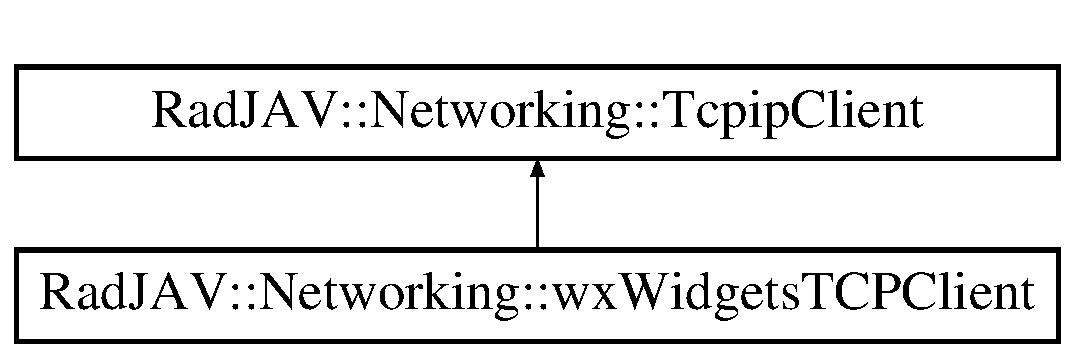
\includegraphics[height=2.000000cm]{class_rad_j_a_v_1_1_networking_1_1_tcpip_client}
\end{center}
\end{figure}
\subsection*{Public Member Functions}
\begin{DoxyCompactItemize}
\item 
\hyperlink{class_rad_j_a_v_1_1_networking_1_1_tcpip_client_aae23fc057bdef796ad8536ddfe9d23f2}{Tcpip\+Client} ()
\item 
virtual bool \hyperlink{class_rad_j_a_v_1_1_networking_1_1_tcpip_client_aba21f2a319d4268bdf04525b1e35ccab}{init} (unsigned short port)=0
\begin{DoxyCompactList}\small\item\em Start the server. \end{DoxyCompactList}\item 
virtual bool \hyperlink{class_rad_j_a_v_1_1_networking_1_1_tcpip_client_ade2497881107c14dd0b3a32ff1f6f669}{connect\+With\+Blocking} (\hyperlink{class_rad_j_a_v_1_1_string}{String} str\+Connect\+To)=0
\begin{DoxyCompactList}\small\item\em Connect to a server while locking the thread. \end{DoxyCompactList}\item 
virtual bool \hyperlink{class_rad_j_a_v_1_1_networking_1_1_tcpip_client_a2125d436db16091fe9c60ed30b34c56e}{connect\+Without\+Blocking} (\hyperlink{class_rad_j_a_v_1_1_string}{String} str\+Connect\+To)=0
\begin{DoxyCompactList}\small\item\em Connect to a server without locking the thread. \end{DoxyCompactList}\item 
virtual bool \hyperlink{class_rad_j_a_v_1_1_networking_1_1_tcpip_client_a0b8da5667dd8c42e8fb358e35b4c8f96}{send\+Float} (float f\+Float)=0
\begin{DoxyCompactList}\small\item\em Send a float to the server. \end{DoxyCompactList}\item 
virtual bool \hyperlink{class_rad_j_a_v_1_1_networking_1_1_tcpip_client_a5f058b50cc9da6de81da6b9f02f2ca24}{send\+Double} (double d\+Double)=0
\begin{DoxyCompactList}\small\item\em Send a double to the server. \end{DoxyCompactList}\item 
virtual bool \hyperlink{class_rad_j_a_v_1_1_networking_1_1_tcpip_client_a55e9334efa84818084a55b8121faaf2f}{send\+Int} (int i\+Int)=0
\begin{DoxyCompactList}\small\item\em Send an int to the server. \end{DoxyCompactList}\item 
virtual bool \hyperlink{class_rad_j_a_v_1_1_networking_1_1_tcpip_client_a2ec37c58d5b4bc9f5460d972a692c52a}{send\+U\+Int} (unsigned int ui\+Int)=0
\begin{DoxyCompactList}\small\item\em Send an unsigned int to the server. \end{DoxyCompactList}\item 
virtual bool \hyperlink{class_rad_j_a_v_1_1_networking_1_1_tcpip_client_aceb6808d0f664dca25ebd56ca1d487ed}{send\+Long} (long l\+Long)=0
\begin{DoxyCompactList}\small\item\em Send a long to the server. \end{DoxyCompactList}\item 
virtual bool \hyperlink{class_rad_j_a_v_1_1_networking_1_1_tcpip_client_a0d74f790e410fbecba34e53d4d47ad9f}{send\+U\+Long} (unsigned long ul\+Long)=0
\begin{DoxyCompactList}\small\item\em Send an unsigned long to the server. \end{DoxyCompactList}\item 
virtual bool \hyperlink{class_rad_j_a_v_1_1_networking_1_1_tcpip_client_ab9d07bcc1dc53c68a1f65bce0fdf613b}{send\+Short} (short s\+Short)=0
\begin{DoxyCompactList}\small\item\em Send a short to the server. \end{DoxyCompactList}\item 
virtual bool \hyperlink{class_rad_j_a_v_1_1_networking_1_1_tcpip_client_a47f22ef4c7e7a8b5a938b8f567eee0ee}{send\+U\+Short} (unsigned short us\+Short)=0
\begin{DoxyCompactList}\small\item\em Send an unsigned short to the server. \end{DoxyCompactList}\item 
virtual bool \hyperlink{class_rad_j_a_v_1_1_networking_1_1_tcpip_client_a03068a5be5c7a1482aacf0c706ad3d9d}{send\+Char} (char c\+Char)=0
\begin{DoxyCompactList}\small\item\em Send a char to the server. \end{DoxyCompactList}\item 
virtual bool \hyperlink{class_rad_j_a_v_1_1_networking_1_1_tcpip_client_a27e9adfc9d218a82cca52bdbe50c8ebf}{send\+U\+Char} (unsigned char uc\+Char)=0
\begin{DoxyCompactList}\small\item\em Send an unsigned char to the server. \end{DoxyCompactList}\item 
virtual bool \hyperlink{class_rad_j_a_v_1_1_networking_1_1_tcpip_client_abb5360e05cb078ed7cdc42bc70ffc3ab}{send\+String} (\hyperlink{class_rad_j_a_v_1_1_string}{String} line)=0
\begin{DoxyCompactList}\small\item\em Send a string to the server. \end{DoxyCompactList}\item 
bool \hyperlink{class_rad_j_a_v_1_1_networking_1_1_tcpip_client_a91ea7348351c25b23e318088f3dad2a8}{H\+T\+T\+P\+Send\+G\+ET} (\hyperlink{class_rad_j_a_v_1_1_string}{String} str\+Retrieve, \hyperlink{class_rad_j_a_v_1_1_string}{String} str\+Headers=\char`\"{}\char`\"{})
\begin{DoxyCompactList}\small\item\em Send an H\+T\+TP request get to the server. \end{DoxyCompactList}\item 
bool \hyperlink{class_rad_j_a_v_1_1_networking_1_1_tcpip_client_aa4b9f535d3b34da9bcfede602b1b09ef}{H\+T\+T\+P\+Send\+P\+O\+ST} (\hyperlink{class_rad_j_a_v_1_1_string}{String} str\+Retrieve, \hyperlink{class_rad_j_a_v_1_1_string}{String} line, \hyperlink{class_rad_j_a_v_1_1_string}{String} str\+Headers, \hyperlink{class_rad_j_a_v_1_1_string}{String} str\+Auth=\char`\"{}\char`\"{})
\begin{DoxyCompactList}\small\item\em Send an H\+T\+TP post request get to the server. \end{DoxyCompactList}\item 
bool \hyperlink{class_rad_j_a_v_1_1_networking_1_1_tcpip_client_a396c8c2729b10ece40ff82b733a89cc0}{H\+T\+T\+P\+Send\+P\+O\+ST} (\hyperlink{class_rad_j_a_v_1_1_string}{String} str\+Content\+Type, \hyperlink{class_rad_j_a_v_1_1_string}{String} str\+Retrieve, \hyperlink{class_rad_j_a_v_1_1_string}{String} line, \hyperlink{class_rad_j_a_v_1_1_string}{String} str\+Headers, \hyperlink{class_rad_j_a_v_1_1_string}{String} str\+Auth=\char`\"{}\char`\"{})
\begin{DoxyCompactList}\small\item\em Send an H\+T\+TP post request get to the server. \end{DoxyCompactList}\item 
\hyperlink{class_rad_j_a_v_1_1_string}{String} \hyperlink{class_rad_j_a_v_1_1_networking_1_1_tcpip_client_ae462f01cc5fbb9bfed9617857015002b}{H\+T\+T\+P\+Parse\+Request} (\hyperlink{class_rad_j_a_v_1_1_string}{String} str\+Content, \hyperlink{class_rad_j_a_v_1_1_string}{String} str\+New\+Line)
\begin{DoxyCompactList}\small\item\em Parse an H\+T\+TP request. \end{DoxyCompactList}\item 
virtual \hyperlink{class_rad_j_a_v_1_1_networking_1_1_t_c_p_response}{T\+C\+P\+Response}$<$ float $>$ \hyperlink{class_rad_j_a_v_1_1_networking_1_1_tcpip_client_acb02176a777a6f3dd05bf48c51e40c7b}{recv\+Float} ()=0
\begin{DoxyCompactList}\small\item\em Receive a float from the server. \end{DoxyCompactList}\item 
virtual \hyperlink{class_rad_j_a_v_1_1_networking_1_1_t_c_p_response}{T\+C\+P\+Response}$<$ double $>$ \hyperlink{class_rad_j_a_v_1_1_networking_1_1_tcpip_client_ab29ea3c5ca1efc4f2d21f724fbadf068}{recv\+Double} ()=0
\begin{DoxyCompactList}\small\item\em Receive a double from the server. \end{DoxyCompactList}\item 
virtual \hyperlink{class_rad_j_a_v_1_1_networking_1_1_t_c_p_response}{T\+C\+P\+Response}$<$ int $>$ \hyperlink{class_rad_j_a_v_1_1_networking_1_1_tcpip_client_a603ea8bc629629e78de34a9fed9ae762}{recv\+Int} ()=0
\begin{DoxyCompactList}\small\item\em Receive an int from the server. \end{DoxyCompactList}\item 
virtual \hyperlink{class_rad_j_a_v_1_1_networking_1_1_t_c_p_response}{T\+C\+P\+Response}$<$ unsigned int $>$ \hyperlink{class_rad_j_a_v_1_1_networking_1_1_tcpip_client_a6baae414514a4577b6e931c7a8b621fa}{recv\+U\+Int} ()=0
\begin{DoxyCompactList}\small\item\em Receive an unsigned int from the server. \end{DoxyCompactList}\item 
virtual \hyperlink{class_rad_j_a_v_1_1_networking_1_1_t_c_p_response}{T\+C\+P\+Response}$<$ long $>$ \hyperlink{class_rad_j_a_v_1_1_networking_1_1_tcpip_client_a3c569e6a3da7e9925647af11a2f6e67e}{recv\+Long} ()=0
\begin{DoxyCompactList}\small\item\em Receive a long from the server. \end{DoxyCompactList}\item 
virtual \hyperlink{class_rad_j_a_v_1_1_networking_1_1_t_c_p_response}{T\+C\+P\+Response}$<$ unsigned long $>$ \hyperlink{class_rad_j_a_v_1_1_networking_1_1_tcpip_client_af87bb449baef6ea793babd5b11cd28e7}{recv\+U\+Long} ()=0
\begin{DoxyCompactList}\small\item\em Receive an unsigned long from the server. \end{DoxyCompactList}\item 
virtual \hyperlink{class_rad_j_a_v_1_1_networking_1_1_t_c_p_response}{T\+C\+P\+Response}$<$ short $>$ \hyperlink{class_rad_j_a_v_1_1_networking_1_1_tcpip_client_a8dad9172da96083b5317d28522f47cba}{recv\+Short} ()=0
\begin{DoxyCompactList}\small\item\em Receive a short from the server. \end{DoxyCompactList}\item 
virtual \hyperlink{class_rad_j_a_v_1_1_networking_1_1_t_c_p_response}{T\+C\+P\+Response}$<$ unsigned short $>$ \hyperlink{class_rad_j_a_v_1_1_networking_1_1_tcpip_client_a85dd74424b331ea12115a2f85a9d2d5b}{recv\+U\+Short} ()=0
\begin{DoxyCompactList}\small\item\em Receive an unsigned short from the server. \end{DoxyCompactList}\item 
virtual \hyperlink{class_rad_j_a_v_1_1_networking_1_1_t_c_p_response}{T\+C\+P\+Response}$<$ char $>$ \hyperlink{class_rad_j_a_v_1_1_networking_1_1_tcpip_client_a831adf67f900d6bb5f57a38b800843b6}{recv\+Char} ()=0
\begin{DoxyCompactList}\small\item\em Receive a char from the server. \end{DoxyCompactList}\item 
virtual \hyperlink{class_rad_j_a_v_1_1_networking_1_1_t_c_p_response}{T\+C\+P\+Response}$<$ unsigned char $>$ \hyperlink{class_rad_j_a_v_1_1_networking_1_1_tcpip_client_aae09d9ff1d6c436b3a624bc94afce148}{recv\+U\+Char} ()=0
\begin{DoxyCompactList}\small\item\em Receive an unsigned char from the server. \end{DoxyCompactList}\item 
virtual \hyperlink{class_rad_j_a_v_1_1_networking_1_1_t_c_p_response}{T\+C\+P\+Response}$<$ char $\ast$ $>$ \hyperlink{class_rad_j_a_v_1_1_networking_1_1_tcpip_client_a595f73382914bb43e70db21bd9f3977a}{recv\+String} (int i\+Length)=0
\begin{DoxyCompactList}\small\item\em Receive a char string from the server. \end{DoxyCompactList}\item 
virtual \hyperlink{class_rad_j_a_v_1_1_networking_1_1_t_c_p_response}{T\+C\+P\+Response}$<$ \hyperlink{class_rad_j_a_v_1_1_string}{String} $>$ \hyperlink{class_rad_j_a_v_1_1_networking_1_1_tcpip_client_ae6ab4734a0461ffe393f6ff2302c0dbe}{recv\+String} ()=0
\begin{DoxyCompactList}\small\item\em Receive a string from the server. \end{DoxyCompactList}\item 
std\+::shared\+\_\+ptr$<$ \hyperlink{class_rad_j_a_v_1_1_networking_1_1_t_c_p_connection}{T\+C\+P\+Connection} $>$ \hyperlink{class_rad_j_a_v_1_1_networking_1_1_tcpip_client_a197d35a074998e466226ea7e43dae060}{get\+Server\+Connection} ()
\begin{DoxyCompactList}\small\item\em Get the connection to the server. \end{DoxyCompactList}\item 
\hyperlink{class_rad_j_a_v_1_1_string}{String} \hyperlink{class_rad_j_a_v_1_1_networking_1_1_tcpip_client_ae03a4a7b2e26c9cf5dbcd788a4694c47}{get\+Server\+IP} ()
\begin{DoxyCompactList}\small\item\em Get the server\textquotesingle{}s ip. \end{DoxyCompactList}\item 
unsigned short \hyperlink{class_rad_j_a_v_1_1_networking_1_1_tcpip_client_a781d9448692dec592e0bf1fa5814a74a}{get\+Port} ()
\begin{DoxyCompactList}\small\item\em Get the port being used. \end{DoxyCompactList}\item 
\hyperlink{class_rad_j_a_v_1_1_string}{String} \hyperlink{class_rad_j_a_v_1_1_networking_1_1_tcpip_client_a06e1ade9aa23df4d251beb2eb96cff4d}{get\+Last\+Error} ()
\begin{DoxyCompactList}\small\item\em Get the last error. \end{DoxyCompactList}\item 
virtual bool \hyperlink{class_rad_j_a_v_1_1_networking_1_1_tcpip_client_a2da2c8b5f71f1d4f16e727d43e26fef8}{close} ()=0
\begin{DoxyCompactList}\small\item\em Close the connection to the server. \end{DoxyCompactList}\end{DoxyCompactItemize}


\subsection{Constructor \& Destructor Documentation}
\index{Rad\+J\+A\+V\+::\+Networking\+::\+Tcpip\+Client@{Rad\+J\+A\+V\+::\+Networking\+::\+Tcpip\+Client}!Tcpip\+Client@{Tcpip\+Client}}
\index{Tcpip\+Client@{Tcpip\+Client}!Rad\+J\+A\+V\+::\+Networking\+::\+Tcpip\+Client@{Rad\+J\+A\+V\+::\+Networking\+::\+Tcpip\+Client}}
\subsubsection[{\texorpdfstring{Tcpip\+Client()}{TcpipClient()}}]{\setlength{\rightskip}{0pt plus 5cm}Rad\+J\+A\+V\+::\+Networking\+::\+Tcpip\+Client\+::\+Tcpip\+Client (
\begin{DoxyParamCaption}
{}
\end{DoxyParamCaption}
)}\hypertarget{class_rad_j_a_v_1_1_networking_1_1_tcpip_client_aae23fc057bdef796ad8536ddfe9d23f2}{}\label{class_rad_j_a_v_1_1_networking_1_1_tcpip_client_aae23fc057bdef796ad8536ddfe9d23f2}


\subsection{Member Function Documentation}
\index{Rad\+J\+A\+V\+::\+Networking\+::\+Tcpip\+Client@{Rad\+J\+A\+V\+::\+Networking\+::\+Tcpip\+Client}!close@{close}}
\index{close@{close}!Rad\+J\+A\+V\+::\+Networking\+::\+Tcpip\+Client@{Rad\+J\+A\+V\+::\+Networking\+::\+Tcpip\+Client}}
\subsubsection[{\texorpdfstring{close()=0}{close()=0}}]{\setlength{\rightskip}{0pt plus 5cm}virtual bool Rad\+J\+A\+V\+::\+Networking\+::\+Tcpip\+Client\+::close (
\begin{DoxyParamCaption}
{}
\end{DoxyParamCaption}
)\hspace{0.3cm}{\ttfamily [pure virtual]}}\hypertarget{class_rad_j_a_v_1_1_networking_1_1_tcpip_client_a2da2c8b5f71f1d4f16e727d43e26fef8}{}\label{class_rad_j_a_v_1_1_networking_1_1_tcpip_client_a2da2c8b5f71f1d4f16e727d43e26fef8}


Close the connection to the server. 

\index{Rad\+J\+A\+V\+::\+Networking\+::\+Tcpip\+Client@{Rad\+J\+A\+V\+::\+Networking\+::\+Tcpip\+Client}!connect\+With\+Blocking@{connect\+With\+Blocking}}
\index{connect\+With\+Blocking@{connect\+With\+Blocking}!Rad\+J\+A\+V\+::\+Networking\+::\+Tcpip\+Client@{Rad\+J\+A\+V\+::\+Networking\+::\+Tcpip\+Client}}
\subsubsection[{\texorpdfstring{connect\+With\+Blocking(\+String str\+Connect\+To)=0}{connectWithBlocking(String strConnectTo)=0}}]{\setlength{\rightskip}{0pt plus 5cm}virtual bool Rad\+J\+A\+V\+::\+Networking\+::\+Tcpip\+Client\+::connect\+With\+Blocking (
\begin{DoxyParamCaption}
\item[{{\bf String}}]{str\+Connect\+To}
\end{DoxyParamCaption}
)\hspace{0.3cm}{\ttfamily [pure virtual]}}\hypertarget{class_rad_j_a_v_1_1_networking_1_1_tcpip_client_ade2497881107c14dd0b3a32ff1f6f669}{}\label{class_rad_j_a_v_1_1_networking_1_1_tcpip_client_ade2497881107c14dd0b3a32ff1f6f669}


Connect to a server while locking the thread. 

\index{Rad\+J\+A\+V\+::\+Networking\+::\+Tcpip\+Client@{Rad\+J\+A\+V\+::\+Networking\+::\+Tcpip\+Client}!connect\+Without\+Blocking@{connect\+Without\+Blocking}}
\index{connect\+Without\+Blocking@{connect\+Without\+Blocking}!Rad\+J\+A\+V\+::\+Networking\+::\+Tcpip\+Client@{Rad\+J\+A\+V\+::\+Networking\+::\+Tcpip\+Client}}
\subsubsection[{\texorpdfstring{connect\+Without\+Blocking(\+String str\+Connect\+To)=0}{connectWithoutBlocking(String strConnectTo)=0}}]{\setlength{\rightskip}{0pt plus 5cm}virtual bool Rad\+J\+A\+V\+::\+Networking\+::\+Tcpip\+Client\+::connect\+Without\+Blocking (
\begin{DoxyParamCaption}
\item[{{\bf String}}]{str\+Connect\+To}
\end{DoxyParamCaption}
)\hspace{0.3cm}{\ttfamily [pure virtual]}}\hypertarget{class_rad_j_a_v_1_1_networking_1_1_tcpip_client_a2125d436db16091fe9c60ed30b34c56e}{}\label{class_rad_j_a_v_1_1_networking_1_1_tcpip_client_a2125d436db16091fe9c60ed30b34c56e}


Connect to a server without locking the thread. 

\index{Rad\+J\+A\+V\+::\+Networking\+::\+Tcpip\+Client@{Rad\+J\+A\+V\+::\+Networking\+::\+Tcpip\+Client}!get\+Last\+Error@{get\+Last\+Error}}
\index{get\+Last\+Error@{get\+Last\+Error}!Rad\+J\+A\+V\+::\+Networking\+::\+Tcpip\+Client@{Rad\+J\+A\+V\+::\+Networking\+::\+Tcpip\+Client}}
\subsubsection[{\texorpdfstring{get\+Last\+Error()}{getLastError()}}]{\setlength{\rightskip}{0pt plus 5cm}{\bf String} Rad\+J\+A\+V\+::\+Networking\+::\+Tcpip\+Client\+::get\+Last\+Error (
\begin{DoxyParamCaption}
{}
\end{DoxyParamCaption}
)}\hypertarget{class_rad_j_a_v_1_1_networking_1_1_tcpip_client_a06e1ade9aa23df4d251beb2eb96cff4d}{}\label{class_rad_j_a_v_1_1_networking_1_1_tcpip_client_a06e1ade9aa23df4d251beb2eb96cff4d}


Get the last error. 

\index{Rad\+J\+A\+V\+::\+Networking\+::\+Tcpip\+Client@{Rad\+J\+A\+V\+::\+Networking\+::\+Tcpip\+Client}!get\+Port@{get\+Port}}
\index{get\+Port@{get\+Port}!Rad\+J\+A\+V\+::\+Networking\+::\+Tcpip\+Client@{Rad\+J\+A\+V\+::\+Networking\+::\+Tcpip\+Client}}
\subsubsection[{\texorpdfstring{get\+Port()}{getPort()}}]{\setlength{\rightskip}{0pt plus 5cm}unsigned short Rad\+J\+A\+V\+::\+Networking\+::\+Tcpip\+Client\+::get\+Port (
\begin{DoxyParamCaption}
{}
\end{DoxyParamCaption}
)}\hypertarget{class_rad_j_a_v_1_1_networking_1_1_tcpip_client_a781d9448692dec592e0bf1fa5814a74a}{}\label{class_rad_j_a_v_1_1_networking_1_1_tcpip_client_a781d9448692dec592e0bf1fa5814a74a}


Get the port being used. 

\index{Rad\+J\+A\+V\+::\+Networking\+::\+Tcpip\+Client@{Rad\+J\+A\+V\+::\+Networking\+::\+Tcpip\+Client}!get\+Server\+Connection@{get\+Server\+Connection}}
\index{get\+Server\+Connection@{get\+Server\+Connection}!Rad\+J\+A\+V\+::\+Networking\+::\+Tcpip\+Client@{Rad\+J\+A\+V\+::\+Networking\+::\+Tcpip\+Client}}
\subsubsection[{\texorpdfstring{get\+Server\+Connection()}{getServerConnection()}}]{\setlength{\rightskip}{0pt plus 5cm}std\+::shared\+\_\+ptr$<$ {\bf T\+C\+P\+Connection} $>$ Rad\+J\+A\+V\+::\+Networking\+::\+Tcpip\+Client\+::get\+Server\+Connection (
\begin{DoxyParamCaption}
{}
\end{DoxyParamCaption}
)}\hypertarget{class_rad_j_a_v_1_1_networking_1_1_tcpip_client_a197d35a074998e466226ea7e43dae060}{}\label{class_rad_j_a_v_1_1_networking_1_1_tcpip_client_a197d35a074998e466226ea7e43dae060}


Get the connection to the server. 

\index{Rad\+J\+A\+V\+::\+Networking\+::\+Tcpip\+Client@{Rad\+J\+A\+V\+::\+Networking\+::\+Tcpip\+Client}!get\+Server\+IP@{get\+Server\+IP}}
\index{get\+Server\+IP@{get\+Server\+IP}!Rad\+J\+A\+V\+::\+Networking\+::\+Tcpip\+Client@{Rad\+J\+A\+V\+::\+Networking\+::\+Tcpip\+Client}}
\subsubsection[{\texorpdfstring{get\+Server\+I\+P()}{getServerIP()}}]{\setlength{\rightskip}{0pt plus 5cm}{\bf String} Rad\+J\+A\+V\+::\+Networking\+::\+Tcpip\+Client\+::get\+Server\+IP (
\begin{DoxyParamCaption}
{}
\end{DoxyParamCaption}
)}\hypertarget{class_rad_j_a_v_1_1_networking_1_1_tcpip_client_ae03a4a7b2e26c9cf5dbcd788a4694c47}{}\label{class_rad_j_a_v_1_1_networking_1_1_tcpip_client_ae03a4a7b2e26c9cf5dbcd788a4694c47}


Get the server\textquotesingle{}s ip. 

\index{Rad\+J\+A\+V\+::\+Networking\+::\+Tcpip\+Client@{Rad\+J\+A\+V\+::\+Networking\+::\+Tcpip\+Client}!H\+T\+T\+P\+Parse\+Request@{H\+T\+T\+P\+Parse\+Request}}
\index{H\+T\+T\+P\+Parse\+Request@{H\+T\+T\+P\+Parse\+Request}!Rad\+J\+A\+V\+::\+Networking\+::\+Tcpip\+Client@{Rad\+J\+A\+V\+::\+Networking\+::\+Tcpip\+Client}}
\subsubsection[{\texorpdfstring{H\+T\+T\+P\+Parse\+Request(\+String str\+Content, String str\+New\+Line)}{HTTPParseRequest(String strContent, String strNewLine)}}]{\setlength{\rightskip}{0pt plus 5cm}{\bf String} Rad\+J\+A\+V\+::\+Networking\+::\+Tcpip\+Client\+::\+H\+T\+T\+P\+Parse\+Request (
\begin{DoxyParamCaption}
\item[{{\bf String}}]{str\+Content, }
\item[{{\bf String}}]{str\+New\+Line}
\end{DoxyParamCaption}
)}\hypertarget{class_rad_j_a_v_1_1_networking_1_1_tcpip_client_ae462f01cc5fbb9bfed9617857015002b}{}\label{class_rad_j_a_v_1_1_networking_1_1_tcpip_client_ae462f01cc5fbb9bfed9617857015002b}


Parse an H\+T\+TP request. 

\index{Rad\+J\+A\+V\+::\+Networking\+::\+Tcpip\+Client@{Rad\+J\+A\+V\+::\+Networking\+::\+Tcpip\+Client}!H\+T\+T\+P\+Send\+G\+ET@{H\+T\+T\+P\+Send\+G\+ET}}
\index{H\+T\+T\+P\+Send\+G\+ET@{H\+T\+T\+P\+Send\+G\+ET}!Rad\+J\+A\+V\+::\+Networking\+::\+Tcpip\+Client@{Rad\+J\+A\+V\+::\+Networking\+::\+Tcpip\+Client}}
\subsubsection[{\texorpdfstring{H\+T\+T\+P\+Send\+G\+E\+T(\+String str\+Retrieve, String str\+Headers="""")}{HTTPSendGET(String strRetrieve, String strHeaders="")}}]{\setlength{\rightskip}{0pt plus 5cm}bool Rad\+J\+A\+V\+::\+Networking\+::\+Tcpip\+Client\+::\+H\+T\+T\+P\+Send\+G\+ET (
\begin{DoxyParamCaption}
\item[{{\bf String}}]{str\+Retrieve, }
\item[{{\bf String}}]{str\+Headers = {\ttfamily \char`\"{}\char`\"{}}}
\end{DoxyParamCaption}
)}\hypertarget{class_rad_j_a_v_1_1_networking_1_1_tcpip_client_a91ea7348351c25b23e318088f3dad2a8}{}\label{class_rad_j_a_v_1_1_networking_1_1_tcpip_client_a91ea7348351c25b23e318088f3dad2a8}


Send an H\+T\+TP request get to the server. 

\index{Rad\+J\+A\+V\+::\+Networking\+::\+Tcpip\+Client@{Rad\+J\+A\+V\+::\+Networking\+::\+Tcpip\+Client}!H\+T\+T\+P\+Send\+P\+O\+ST@{H\+T\+T\+P\+Send\+P\+O\+ST}}
\index{H\+T\+T\+P\+Send\+P\+O\+ST@{H\+T\+T\+P\+Send\+P\+O\+ST}!Rad\+J\+A\+V\+::\+Networking\+::\+Tcpip\+Client@{Rad\+J\+A\+V\+::\+Networking\+::\+Tcpip\+Client}}
\subsubsection[{\texorpdfstring{H\+T\+T\+P\+Send\+P\+O\+S\+T(\+String str\+Retrieve, String line, String str\+Headers, String str\+Auth="""")}{HTTPSendPOST(String strRetrieve, String line, String strHeaders, String strAuth="")}}]{\setlength{\rightskip}{0pt plus 5cm}bool Rad\+J\+A\+V\+::\+Networking\+::\+Tcpip\+Client\+::\+H\+T\+T\+P\+Send\+P\+O\+ST (
\begin{DoxyParamCaption}
\item[{{\bf String}}]{str\+Retrieve, }
\item[{{\bf String}}]{line, }
\item[{{\bf String}}]{str\+Headers, }
\item[{{\bf String}}]{str\+Auth = {\ttfamily \char`\"{}\char`\"{}}}
\end{DoxyParamCaption}
)}\hypertarget{class_rad_j_a_v_1_1_networking_1_1_tcpip_client_aa4b9f535d3b34da9bcfede602b1b09ef}{}\label{class_rad_j_a_v_1_1_networking_1_1_tcpip_client_aa4b9f535d3b34da9bcfede602b1b09ef}


Send an H\+T\+TP post request get to the server. 

\index{Rad\+J\+A\+V\+::\+Networking\+::\+Tcpip\+Client@{Rad\+J\+A\+V\+::\+Networking\+::\+Tcpip\+Client}!H\+T\+T\+P\+Send\+P\+O\+ST@{H\+T\+T\+P\+Send\+P\+O\+ST}}
\index{H\+T\+T\+P\+Send\+P\+O\+ST@{H\+T\+T\+P\+Send\+P\+O\+ST}!Rad\+J\+A\+V\+::\+Networking\+::\+Tcpip\+Client@{Rad\+J\+A\+V\+::\+Networking\+::\+Tcpip\+Client}}
\subsubsection[{\texorpdfstring{H\+T\+T\+P\+Send\+P\+O\+S\+T(\+String str\+Content\+Type, String str\+Retrieve, String line, String str\+Headers, String str\+Auth="""")}{HTTPSendPOST(String strContentType, String strRetrieve, String line, String strHeaders, String strAuth="")}}]{\setlength{\rightskip}{0pt plus 5cm}bool Rad\+J\+A\+V\+::\+Networking\+::\+Tcpip\+Client\+::\+H\+T\+T\+P\+Send\+P\+O\+ST (
\begin{DoxyParamCaption}
\item[{{\bf String}}]{str\+Content\+Type, }
\item[{{\bf String}}]{str\+Retrieve, }
\item[{{\bf String}}]{line, }
\item[{{\bf String}}]{str\+Headers, }
\item[{{\bf String}}]{str\+Auth = {\ttfamily \char`\"{}\char`\"{}}}
\end{DoxyParamCaption}
)}\hypertarget{class_rad_j_a_v_1_1_networking_1_1_tcpip_client_a396c8c2729b10ece40ff82b733a89cc0}{}\label{class_rad_j_a_v_1_1_networking_1_1_tcpip_client_a396c8c2729b10ece40ff82b733a89cc0}


Send an H\+T\+TP post request get to the server. 

\index{Rad\+J\+A\+V\+::\+Networking\+::\+Tcpip\+Client@{Rad\+J\+A\+V\+::\+Networking\+::\+Tcpip\+Client}!init@{init}}
\index{init@{init}!Rad\+J\+A\+V\+::\+Networking\+::\+Tcpip\+Client@{Rad\+J\+A\+V\+::\+Networking\+::\+Tcpip\+Client}}
\subsubsection[{\texorpdfstring{init(unsigned short port)=0}{init(unsigned short port)=0}}]{\setlength{\rightskip}{0pt plus 5cm}virtual bool Rad\+J\+A\+V\+::\+Networking\+::\+Tcpip\+Client\+::init (
\begin{DoxyParamCaption}
\item[{unsigned short}]{port}
\end{DoxyParamCaption}
)\hspace{0.3cm}{\ttfamily [pure virtual]}}\hypertarget{class_rad_j_a_v_1_1_networking_1_1_tcpip_client_aba21f2a319d4268bdf04525b1e35ccab}{}\label{class_rad_j_a_v_1_1_networking_1_1_tcpip_client_aba21f2a319d4268bdf04525b1e35ccab}


Start the server. 

\index{Rad\+J\+A\+V\+::\+Networking\+::\+Tcpip\+Client@{Rad\+J\+A\+V\+::\+Networking\+::\+Tcpip\+Client}!recv\+Char@{recv\+Char}}
\index{recv\+Char@{recv\+Char}!Rad\+J\+A\+V\+::\+Networking\+::\+Tcpip\+Client@{Rad\+J\+A\+V\+::\+Networking\+::\+Tcpip\+Client}}
\subsubsection[{\texorpdfstring{recv\+Char()=0}{recvChar()=0}}]{\setlength{\rightskip}{0pt plus 5cm}virtual {\bf T\+C\+P\+Response}$<$char$>$ Rad\+J\+A\+V\+::\+Networking\+::\+Tcpip\+Client\+::recv\+Char (
\begin{DoxyParamCaption}
{}
\end{DoxyParamCaption}
)\hspace{0.3cm}{\ttfamily [pure virtual]}}\hypertarget{class_rad_j_a_v_1_1_networking_1_1_tcpip_client_a831adf67f900d6bb5f57a38b800843b6}{}\label{class_rad_j_a_v_1_1_networking_1_1_tcpip_client_a831adf67f900d6bb5f57a38b800843b6}


Receive a char from the server. 

\index{Rad\+J\+A\+V\+::\+Networking\+::\+Tcpip\+Client@{Rad\+J\+A\+V\+::\+Networking\+::\+Tcpip\+Client}!recv\+Double@{recv\+Double}}
\index{recv\+Double@{recv\+Double}!Rad\+J\+A\+V\+::\+Networking\+::\+Tcpip\+Client@{Rad\+J\+A\+V\+::\+Networking\+::\+Tcpip\+Client}}
\subsubsection[{\texorpdfstring{recv\+Double()=0}{recvDouble()=0}}]{\setlength{\rightskip}{0pt plus 5cm}virtual {\bf T\+C\+P\+Response}$<$double$>$ Rad\+J\+A\+V\+::\+Networking\+::\+Tcpip\+Client\+::recv\+Double (
\begin{DoxyParamCaption}
{}
\end{DoxyParamCaption}
)\hspace{0.3cm}{\ttfamily [pure virtual]}}\hypertarget{class_rad_j_a_v_1_1_networking_1_1_tcpip_client_ab29ea3c5ca1efc4f2d21f724fbadf068}{}\label{class_rad_j_a_v_1_1_networking_1_1_tcpip_client_ab29ea3c5ca1efc4f2d21f724fbadf068}


Receive a double from the server. 

\index{Rad\+J\+A\+V\+::\+Networking\+::\+Tcpip\+Client@{Rad\+J\+A\+V\+::\+Networking\+::\+Tcpip\+Client}!recv\+Float@{recv\+Float}}
\index{recv\+Float@{recv\+Float}!Rad\+J\+A\+V\+::\+Networking\+::\+Tcpip\+Client@{Rad\+J\+A\+V\+::\+Networking\+::\+Tcpip\+Client}}
\subsubsection[{\texorpdfstring{recv\+Float()=0}{recvFloat()=0}}]{\setlength{\rightskip}{0pt plus 5cm}virtual {\bf T\+C\+P\+Response}$<$float$>$ Rad\+J\+A\+V\+::\+Networking\+::\+Tcpip\+Client\+::recv\+Float (
\begin{DoxyParamCaption}
{}
\end{DoxyParamCaption}
)\hspace{0.3cm}{\ttfamily [pure virtual]}}\hypertarget{class_rad_j_a_v_1_1_networking_1_1_tcpip_client_acb02176a777a6f3dd05bf48c51e40c7b}{}\label{class_rad_j_a_v_1_1_networking_1_1_tcpip_client_acb02176a777a6f3dd05bf48c51e40c7b}


Receive a float from the server. 

\index{Rad\+J\+A\+V\+::\+Networking\+::\+Tcpip\+Client@{Rad\+J\+A\+V\+::\+Networking\+::\+Tcpip\+Client}!recv\+Int@{recv\+Int}}
\index{recv\+Int@{recv\+Int}!Rad\+J\+A\+V\+::\+Networking\+::\+Tcpip\+Client@{Rad\+J\+A\+V\+::\+Networking\+::\+Tcpip\+Client}}
\subsubsection[{\texorpdfstring{recv\+Int()=0}{recvInt()=0}}]{\setlength{\rightskip}{0pt plus 5cm}virtual {\bf T\+C\+P\+Response}$<$int$>$ Rad\+J\+A\+V\+::\+Networking\+::\+Tcpip\+Client\+::recv\+Int (
\begin{DoxyParamCaption}
{}
\end{DoxyParamCaption}
)\hspace{0.3cm}{\ttfamily [pure virtual]}}\hypertarget{class_rad_j_a_v_1_1_networking_1_1_tcpip_client_a603ea8bc629629e78de34a9fed9ae762}{}\label{class_rad_j_a_v_1_1_networking_1_1_tcpip_client_a603ea8bc629629e78de34a9fed9ae762}


Receive an int from the server. 

\index{Rad\+J\+A\+V\+::\+Networking\+::\+Tcpip\+Client@{Rad\+J\+A\+V\+::\+Networking\+::\+Tcpip\+Client}!recv\+Long@{recv\+Long}}
\index{recv\+Long@{recv\+Long}!Rad\+J\+A\+V\+::\+Networking\+::\+Tcpip\+Client@{Rad\+J\+A\+V\+::\+Networking\+::\+Tcpip\+Client}}
\subsubsection[{\texorpdfstring{recv\+Long()=0}{recvLong()=0}}]{\setlength{\rightskip}{0pt plus 5cm}virtual {\bf T\+C\+P\+Response}$<$long$>$ Rad\+J\+A\+V\+::\+Networking\+::\+Tcpip\+Client\+::recv\+Long (
\begin{DoxyParamCaption}
{}
\end{DoxyParamCaption}
)\hspace{0.3cm}{\ttfamily [pure virtual]}}\hypertarget{class_rad_j_a_v_1_1_networking_1_1_tcpip_client_a3c569e6a3da7e9925647af11a2f6e67e}{}\label{class_rad_j_a_v_1_1_networking_1_1_tcpip_client_a3c569e6a3da7e9925647af11a2f6e67e}


Receive a long from the server. 

\index{Rad\+J\+A\+V\+::\+Networking\+::\+Tcpip\+Client@{Rad\+J\+A\+V\+::\+Networking\+::\+Tcpip\+Client}!recv\+Short@{recv\+Short}}
\index{recv\+Short@{recv\+Short}!Rad\+J\+A\+V\+::\+Networking\+::\+Tcpip\+Client@{Rad\+J\+A\+V\+::\+Networking\+::\+Tcpip\+Client}}
\subsubsection[{\texorpdfstring{recv\+Short()=0}{recvShort()=0}}]{\setlength{\rightskip}{0pt plus 5cm}virtual {\bf T\+C\+P\+Response}$<$short$>$ Rad\+J\+A\+V\+::\+Networking\+::\+Tcpip\+Client\+::recv\+Short (
\begin{DoxyParamCaption}
{}
\end{DoxyParamCaption}
)\hspace{0.3cm}{\ttfamily [pure virtual]}}\hypertarget{class_rad_j_a_v_1_1_networking_1_1_tcpip_client_a8dad9172da96083b5317d28522f47cba}{}\label{class_rad_j_a_v_1_1_networking_1_1_tcpip_client_a8dad9172da96083b5317d28522f47cba}


Receive a short from the server. 

\index{Rad\+J\+A\+V\+::\+Networking\+::\+Tcpip\+Client@{Rad\+J\+A\+V\+::\+Networking\+::\+Tcpip\+Client}!recv\+String@{recv\+String}}
\index{recv\+String@{recv\+String}!Rad\+J\+A\+V\+::\+Networking\+::\+Tcpip\+Client@{Rad\+J\+A\+V\+::\+Networking\+::\+Tcpip\+Client}}
\subsubsection[{\texorpdfstring{recv\+String(int i\+Length)=0}{recvString(int iLength)=0}}]{\setlength{\rightskip}{0pt plus 5cm}virtual {\bf T\+C\+P\+Response}$<$char $\ast$$>$ Rad\+J\+A\+V\+::\+Networking\+::\+Tcpip\+Client\+::recv\+String (
\begin{DoxyParamCaption}
\item[{int}]{i\+Length}
\end{DoxyParamCaption}
)\hspace{0.3cm}{\ttfamily [pure virtual]}}\hypertarget{class_rad_j_a_v_1_1_networking_1_1_tcpip_client_a595f73382914bb43e70db21bd9f3977a}{}\label{class_rad_j_a_v_1_1_networking_1_1_tcpip_client_a595f73382914bb43e70db21bd9f3977a}


Receive a char string from the server. 

\index{Rad\+J\+A\+V\+::\+Networking\+::\+Tcpip\+Client@{Rad\+J\+A\+V\+::\+Networking\+::\+Tcpip\+Client}!recv\+String@{recv\+String}}
\index{recv\+String@{recv\+String}!Rad\+J\+A\+V\+::\+Networking\+::\+Tcpip\+Client@{Rad\+J\+A\+V\+::\+Networking\+::\+Tcpip\+Client}}
\subsubsection[{\texorpdfstring{recv\+String()=0}{recvString()=0}}]{\setlength{\rightskip}{0pt plus 5cm}virtual {\bf T\+C\+P\+Response}$<${\bf String}$>$ Rad\+J\+A\+V\+::\+Networking\+::\+Tcpip\+Client\+::recv\+String (
\begin{DoxyParamCaption}
{}
\end{DoxyParamCaption}
)\hspace{0.3cm}{\ttfamily [pure virtual]}}\hypertarget{class_rad_j_a_v_1_1_networking_1_1_tcpip_client_ae6ab4734a0461ffe393f6ff2302c0dbe}{}\label{class_rad_j_a_v_1_1_networking_1_1_tcpip_client_ae6ab4734a0461ffe393f6ff2302c0dbe}


Receive a string from the server. 

\index{Rad\+J\+A\+V\+::\+Networking\+::\+Tcpip\+Client@{Rad\+J\+A\+V\+::\+Networking\+::\+Tcpip\+Client}!recv\+U\+Char@{recv\+U\+Char}}
\index{recv\+U\+Char@{recv\+U\+Char}!Rad\+J\+A\+V\+::\+Networking\+::\+Tcpip\+Client@{Rad\+J\+A\+V\+::\+Networking\+::\+Tcpip\+Client}}
\subsubsection[{\texorpdfstring{recv\+U\+Char()=0}{recvUChar()=0}}]{\setlength{\rightskip}{0pt plus 5cm}virtual {\bf T\+C\+P\+Response}$<$unsigned char$>$ Rad\+J\+A\+V\+::\+Networking\+::\+Tcpip\+Client\+::recv\+U\+Char (
\begin{DoxyParamCaption}
{}
\end{DoxyParamCaption}
)\hspace{0.3cm}{\ttfamily [pure virtual]}}\hypertarget{class_rad_j_a_v_1_1_networking_1_1_tcpip_client_aae09d9ff1d6c436b3a624bc94afce148}{}\label{class_rad_j_a_v_1_1_networking_1_1_tcpip_client_aae09d9ff1d6c436b3a624bc94afce148}


Receive an unsigned char from the server. 

\index{Rad\+J\+A\+V\+::\+Networking\+::\+Tcpip\+Client@{Rad\+J\+A\+V\+::\+Networking\+::\+Tcpip\+Client}!recv\+U\+Int@{recv\+U\+Int}}
\index{recv\+U\+Int@{recv\+U\+Int}!Rad\+J\+A\+V\+::\+Networking\+::\+Tcpip\+Client@{Rad\+J\+A\+V\+::\+Networking\+::\+Tcpip\+Client}}
\subsubsection[{\texorpdfstring{recv\+U\+Int()=0}{recvUInt()=0}}]{\setlength{\rightskip}{0pt plus 5cm}virtual {\bf T\+C\+P\+Response}$<$unsigned int$>$ Rad\+J\+A\+V\+::\+Networking\+::\+Tcpip\+Client\+::recv\+U\+Int (
\begin{DoxyParamCaption}
{}
\end{DoxyParamCaption}
)\hspace{0.3cm}{\ttfamily [pure virtual]}}\hypertarget{class_rad_j_a_v_1_1_networking_1_1_tcpip_client_a6baae414514a4577b6e931c7a8b621fa}{}\label{class_rad_j_a_v_1_1_networking_1_1_tcpip_client_a6baae414514a4577b6e931c7a8b621fa}


Receive an unsigned int from the server. 

\index{Rad\+J\+A\+V\+::\+Networking\+::\+Tcpip\+Client@{Rad\+J\+A\+V\+::\+Networking\+::\+Tcpip\+Client}!recv\+U\+Long@{recv\+U\+Long}}
\index{recv\+U\+Long@{recv\+U\+Long}!Rad\+J\+A\+V\+::\+Networking\+::\+Tcpip\+Client@{Rad\+J\+A\+V\+::\+Networking\+::\+Tcpip\+Client}}
\subsubsection[{\texorpdfstring{recv\+U\+Long()=0}{recvULong()=0}}]{\setlength{\rightskip}{0pt plus 5cm}virtual {\bf T\+C\+P\+Response}$<$unsigned long$>$ Rad\+J\+A\+V\+::\+Networking\+::\+Tcpip\+Client\+::recv\+U\+Long (
\begin{DoxyParamCaption}
{}
\end{DoxyParamCaption}
)\hspace{0.3cm}{\ttfamily [pure virtual]}}\hypertarget{class_rad_j_a_v_1_1_networking_1_1_tcpip_client_af87bb449baef6ea793babd5b11cd28e7}{}\label{class_rad_j_a_v_1_1_networking_1_1_tcpip_client_af87bb449baef6ea793babd5b11cd28e7}


Receive an unsigned long from the server. 

\index{Rad\+J\+A\+V\+::\+Networking\+::\+Tcpip\+Client@{Rad\+J\+A\+V\+::\+Networking\+::\+Tcpip\+Client}!recv\+U\+Short@{recv\+U\+Short}}
\index{recv\+U\+Short@{recv\+U\+Short}!Rad\+J\+A\+V\+::\+Networking\+::\+Tcpip\+Client@{Rad\+J\+A\+V\+::\+Networking\+::\+Tcpip\+Client}}
\subsubsection[{\texorpdfstring{recv\+U\+Short()=0}{recvUShort()=0}}]{\setlength{\rightskip}{0pt plus 5cm}virtual {\bf T\+C\+P\+Response}$<$unsigned short$>$ Rad\+J\+A\+V\+::\+Networking\+::\+Tcpip\+Client\+::recv\+U\+Short (
\begin{DoxyParamCaption}
{}
\end{DoxyParamCaption}
)\hspace{0.3cm}{\ttfamily [pure virtual]}}\hypertarget{class_rad_j_a_v_1_1_networking_1_1_tcpip_client_a85dd74424b331ea12115a2f85a9d2d5b}{}\label{class_rad_j_a_v_1_1_networking_1_1_tcpip_client_a85dd74424b331ea12115a2f85a9d2d5b}


Receive an unsigned short from the server. 

\index{Rad\+J\+A\+V\+::\+Networking\+::\+Tcpip\+Client@{Rad\+J\+A\+V\+::\+Networking\+::\+Tcpip\+Client}!send\+Char@{send\+Char}}
\index{send\+Char@{send\+Char}!Rad\+J\+A\+V\+::\+Networking\+::\+Tcpip\+Client@{Rad\+J\+A\+V\+::\+Networking\+::\+Tcpip\+Client}}
\subsubsection[{\texorpdfstring{send\+Char(char c\+Char)=0}{sendChar(char cChar)=0}}]{\setlength{\rightskip}{0pt plus 5cm}virtual bool Rad\+J\+A\+V\+::\+Networking\+::\+Tcpip\+Client\+::send\+Char (
\begin{DoxyParamCaption}
\item[{char}]{c\+Char}
\end{DoxyParamCaption}
)\hspace{0.3cm}{\ttfamily [pure virtual]}}\hypertarget{class_rad_j_a_v_1_1_networking_1_1_tcpip_client_a03068a5be5c7a1482aacf0c706ad3d9d}{}\label{class_rad_j_a_v_1_1_networking_1_1_tcpip_client_a03068a5be5c7a1482aacf0c706ad3d9d}


Send a char to the server. 



Implemented in \hyperlink{class_rad_j_a_v_1_1_networking_1_1wx_widgets_t_c_p_client_a3fdaa69183625a5555d99da0a32c6700}{Rad\+J\+A\+V\+::\+Networking\+::wx\+Widgets\+T\+C\+P\+Client}.

\index{Rad\+J\+A\+V\+::\+Networking\+::\+Tcpip\+Client@{Rad\+J\+A\+V\+::\+Networking\+::\+Tcpip\+Client}!send\+Double@{send\+Double}}
\index{send\+Double@{send\+Double}!Rad\+J\+A\+V\+::\+Networking\+::\+Tcpip\+Client@{Rad\+J\+A\+V\+::\+Networking\+::\+Tcpip\+Client}}
\subsubsection[{\texorpdfstring{send\+Double(double d\+Double)=0}{sendDouble(double dDouble)=0}}]{\setlength{\rightskip}{0pt plus 5cm}virtual bool Rad\+J\+A\+V\+::\+Networking\+::\+Tcpip\+Client\+::send\+Double (
\begin{DoxyParamCaption}
\item[{double}]{d\+Double}
\end{DoxyParamCaption}
)\hspace{0.3cm}{\ttfamily [pure virtual]}}\hypertarget{class_rad_j_a_v_1_1_networking_1_1_tcpip_client_a5f058b50cc9da6de81da6b9f02f2ca24}{}\label{class_rad_j_a_v_1_1_networking_1_1_tcpip_client_a5f058b50cc9da6de81da6b9f02f2ca24}


Send a double to the server. 



Implemented in \hyperlink{class_rad_j_a_v_1_1_networking_1_1wx_widgets_t_c_p_client_afb57ef92f150833532015d14475a5ae1}{Rad\+J\+A\+V\+::\+Networking\+::wx\+Widgets\+T\+C\+P\+Client}.

\index{Rad\+J\+A\+V\+::\+Networking\+::\+Tcpip\+Client@{Rad\+J\+A\+V\+::\+Networking\+::\+Tcpip\+Client}!send\+Float@{send\+Float}}
\index{send\+Float@{send\+Float}!Rad\+J\+A\+V\+::\+Networking\+::\+Tcpip\+Client@{Rad\+J\+A\+V\+::\+Networking\+::\+Tcpip\+Client}}
\subsubsection[{\texorpdfstring{send\+Float(float f\+Float)=0}{sendFloat(float fFloat)=0}}]{\setlength{\rightskip}{0pt plus 5cm}virtual bool Rad\+J\+A\+V\+::\+Networking\+::\+Tcpip\+Client\+::send\+Float (
\begin{DoxyParamCaption}
\item[{float}]{f\+Float}
\end{DoxyParamCaption}
)\hspace{0.3cm}{\ttfamily [pure virtual]}}\hypertarget{class_rad_j_a_v_1_1_networking_1_1_tcpip_client_a0b8da5667dd8c42e8fb358e35b4c8f96}{}\label{class_rad_j_a_v_1_1_networking_1_1_tcpip_client_a0b8da5667dd8c42e8fb358e35b4c8f96}


Send a float to the server. 



Implemented in \hyperlink{class_rad_j_a_v_1_1_networking_1_1wx_widgets_t_c_p_client_ad683dafeb275ab9b1dd60bcd1f177107}{Rad\+J\+A\+V\+::\+Networking\+::wx\+Widgets\+T\+C\+P\+Client}.

\index{Rad\+J\+A\+V\+::\+Networking\+::\+Tcpip\+Client@{Rad\+J\+A\+V\+::\+Networking\+::\+Tcpip\+Client}!send\+Int@{send\+Int}}
\index{send\+Int@{send\+Int}!Rad\+J\+A\+V\+::\+Networking\+::\+Tcpip\+Client@{Rad\+J\+A\+V\+::\+Networking\+::\+Tcpip\+Client}}
\subsubsection[{\texorpdfstring{send\+Int(int i\+Int)=0}{sendInt(int iInt)=0}}]{\setlength{\rightskip}{0pt plus 5cm}virtual bool Rad\+J\+A\+V\+::\+Networking\+::\+Tcpip\+Client\+::send\+Int (
\begin{DoxyParamCaption}
\item[{int}]{i\+Int}
\end{DoxyParamCaption}
)\hspace{0.3cm}{\ttfamily [pure virtual]}}\hypertarget{class_rad_j_a_v_1_1_networking_1_1_tcpip_client_a55e9334efa84818084a55b8121faaf2f}{}\label{class_rad_j_a_v_1_1_networking_1_1_tcpip_client_a55e9334efa84818084a55b8121faaf2f}


Send an int to the server. 



Implemented in \hyperlink{class_rad_j_a_v_1_1_networking_1_1wx_widgets_t_c_p_client_a8463c6778160ef13bfd87dac47676614}{Rad\+J\+A\+V\+::\+Networking\+::wx\+Widgets\+T\+C\+P\+Client}.

\index{Rad\+J\+A\+V\+::\+Networking\+::\+Tcpip\+Client@{Rad\+J\+A\+V\+::\+Networking\+::\+Tcpip\+Client}!send\+Long@{send\+Long}}
\index{send\+Long@{send\+Long}!Rad\+J\+A\+V\+::\+Networking\+::\+Tcpip\+Client@{Rad\+J\+A\+V\+::\+Networking\+::\+Tcpip\+Client}}
\subsubsection[{\texorpdfstring{send\+Long(long l\+Long)=0}{sendLong(long lLong)=0}}]{\setlength{\rightskip}{0pt plus 5cm}virtual bool Rad\+J\+A\+V\+::\+Networking\+::\+Tcpip\+Client\+::send\+Long (
\begin{DoxyParamCaption}
\item[{long}]{l\+Long}
\end{DoxyParamCaption}
)\hspace{0.3cm}{\ttfamily [pure virtual]}}\hypertarget{class_rad_j_a_v_1_1_networking_1_1_tcpip_client_aceb6808d0f664dca25ebd56ca1d487ed}{}\label{class_rad_j_a_v_1_1_networking_1_1_tcpip_client_aceb6808d0f664dca25ebd56ca1d487ed}


Send a long to the server. 



Implemented in \hyperlink{class_rad_j_a_v_1_1_networking_1_1wx_widgets_t_c_p_client_aaa40b254965bfc2b4d3b27877602da9c}{Rad\+J\+A\+V\+::\+Networking\+::wx\+Widgets\+T\+C\+P\+Client}.

\index{Rad\+J\+A\+V\+::\+Networking\+::\+Tcpip\+Client@{Rad\+J\+A\+V\+::\+Networking\+::\+Tcpip\+Client}!send\+Short@{send\+Short}}
\index{send\+Short@{send\+Short}!Rad\+J\+A\+V\+::\+Networking\+::\+Tcpip\+Client@{Rad\+J\+A\+V\+::\+Networking\+::\+Tcpip\+Client}}
\subsubsection[{\texorpdfstring{send\+Short(short s\+Short)=0}{sendShort(short sShort)=0}}]{\setlength{\rightskip}{0pt plus 5cm}virtual bool Rad\+J\+A\+V\+::\+Networking\+::\+Tcpip\+Client\+::send\+Short (
\begin{DoxyParamCaption}
\item[{short}]{s\+Short}
\end{DoxyParamCaption}
)\hspace{0.3cm}{\ttfamily [pure virtual]}}\hypertarget{class_rad_j_a_v_1_1_networking_1_1_tcpip_client_ab9d07bcc1dc53c68a1f65bce0fdf613b}{}\label{class_rad_j_a_v_1_1_networking_1_1_tcpip_client_ab9d07bcc1dc53c68a1f65bce0fdf613b}


Send a short to the server. 



Implemented in \hyperlink{class_rad_j_a_v_1_1_networking_1_1wx_widgets_t_c_p_client_afeb26d6478b3c8f869f67c41e3105bec}{Rad\+J\+A\+V\+::\+Networking\+::wx\+Widgets\+T\+C\+P\+Client}.

\index{Rad\+J\+A\+V\+::\+Networking\+::\+Tcpip\+Client@{Rad\+J\+A\+V\+::\+Networking\+::\+Tcpip\+Client}!send\+String@{send\+String}}
\index{send\+String@{send\+String}!Rad\+J\+A\+V\+::\+Networking\+::\+Tcpip\+Client@{Rad\+J\+A\+V\+::\+Networking\+::\+Tcpip\+Client}}
\subsubsection[{\texorpdfstring{send\+String(\+String line)=0}{sendString(String line)=0}}]{\setlength{\rightskip}{0pt plus 5cm}virtual bool Rad\+J\+A\+V\+::\+Networking\+::\+Tcpip\+Client\+::send\+String (
\begin{DoxyParamCaption}
\item[{{\bf String}}]{line}
\end{DoxyParamCaption}
)\hspace{0.3cm}{\ttfamily [pure virtual]}}\hypertarget{class_rad_j_a_v_1_1_networking_1_1_tcpip_client_abb5360e05cb078ed7cdc42bc70ffc3ab}{}\label{class_rad_j_a_v_1_1_networking_1_1_tcpip_client_abb5360e05cb078ed7cdc42bc70ffc3ab}


Send a string to the server. 



Implemented in \hyperlink{class_rad_j_a_v_1_1_networking_1_1wx_widgets_t_c_p_client_a2282375d71da7b7d38ef06a977e46827}{Rad\+J\+A\+V\+::\+Networking\+::wx\+Widgets\+T\+C\+P\+Client}.

\index{Rad\+J\+A\+V\+::\+Networking\+::\+Tcpip\+Client@{Rad\+J\+A\+V\+::\+Networking\+::\+Tcpip\+Client}!send\+U\+Char@{send\+U\+Char}}
\index{send\+U\+Char@{send\+U\+Char}!Rad\+J\+A\+V\+::\+Networking\+::\+Tcpip\+Client@{Rad\+J\+A\+V\+::\+Networking\+::\+Tcpip\+Client}}
\subsubsection[{\texorpdfstring{send\+U\+Char(unsigned char uc\+Char)=0}{sendUChar(unsigned char ucChar)=0}}]{\setlength{\rightskip}{0pt plus 5cm}virtual bool Rad\+J\+A\+V\+::\+Networking\+::\+Tcpip\+Client\+::send\+U\+Char (
\begin{DoxyParamCaption}
\item[{unsigned char}]{uc\+Char}
\end{DoxyParamCaption}
)\hspace{0.3cm}{\ttfamily [pure virtual]}}\hypertarget{class_rad_j_a_v_1_1_networking_1_1_tcpip_client_a27e9adfc9d218a82cca52bdbe50c8ebf}{}\label{class_rad_j_a_v_1_1_networking_1_1_tcpip_client_a27e9adfc9d218a82cca52bdbe50c8ebf}


Send an unsigned char to the server. 



Implemented in \hyperlink{class_rad_j_a_v_1_1_networking_1_1wx_widgets_t_c_p_client_ae50f5c377cd8116159f7afa5e7f0bbd5}{Rad\+J\+A\+V\+::\+Networking\+::wx\+Widgets\+T\+C\+P\+Client}.

\index{Rad\+J\+A\+V\+::\+Networking\+::\+Tcpip\+Client@{Rad\+J\+A\+V\+::\+Networking\+::\+Tcpip\+Client}!send\+U\+Int@{send\+U\+Int}}
\index{send\+U\+Int@{send\+U\+Int}!Rad\+J\+A\+V\+::\+Networking\+::\+Tcpip\+Client@{Rad\+J\+A\+V\+::\+Networking\+::\+Tcpip\+Client}}
\subsubsection[{\texorpdfstring{send\+U\+Int(unsigned int ui\+Int)=0}{sendUInt(unsigned int uiInt)=0}}]{\setlength{\rightskip}{0pt plus 5cm}virtual bool Rad\+J\+A\+V\+::\+Networking\+::\+Tcpip\+Client\+::send\+U\+Int (
\begin{DoxyParamCaption}
\item[{unsigned int}]{ui\+Int}
\end{DoxyParamCaption}
)\hspace{0.3cm}{\ttfamily [pure virtual]}}\hypertarget{class_rad_j_a_v_1_1_networking_1_1_tcpip_client_a2ec37c58d5b4bc9f5460d972a692c52a}{}\label{class_rad_j_a_v_1_1_networking_1_1_tcpip_client_a2ec37c58d5b4bc9f5460d972a692c52a}


Send an unsigned int to the server. 



Implemented in \hyperlink{class_rad_j_a_v_1_1_networking_1_1wx_widgets_t_c_p_client_a4dd19f4c7b18c6599972f238f6021580}{Rad\+J\+A\+V\+::\+Networking\+::wx\+Widgets\+T\+C\+P\+Client}.

\index{Rad\+J\+A\+V\+::\+Networking\+::\+Tcpip\+Client@{Rad\+J\+A\+V\+::\+Networking\+::\+Tcpip\+Client}!send\+U\+Long@{send\+U\+Long}}
\index{send\+U\+Long@{send\+U\+Long}!Rad\+J\+A\+V\+::\+Networking\+::\+Tcpip\+Client@{Rad\+J\+A\+V\+::\+Networking\+::\+Tcpip\+Client}}
\subsubsection[{\texorpdfstring{send\+U\+Long(unsigned long ul\+Long)=0}{sendULong(unsigned long ulLong)=0}}]{\setlength{\rightskip}{0pt plus 5cm}virtual bool Rad\+J\+A\+V\+::\+Networking\+::\+Tcpip\+Client\+::send\+U\+Long (
\begin{DoxyParamCaption}
\item[{unsigned long}]{ul\+Long}
\end{DoxyParamCaption}
)\hspace{0.3cm}{\ttfamily [pure virtual]}}\hypertarget{class_rad_j_a_v_1_1_networking_1_1_tcpip_client_a0d74f790e410fbecba34e53d4d47ad9f}{}\label{class_rad_j_a_v_1_1_networking_1_1_tcpip_client_a0d74f790e410fbecba34e53d4d47ad9f}


Send an unsigned long to the server. 



Implemented in \hyperlink{class_rad_j_a_v_1_1_networking_1_1wx_widgets_t_c_p_client_a8440ad8c4446f1525329cfe40d630ead}{Rad\+J\+A\+V\+::\+Networking\+::wx\+Widgets\+T\+C\+P\+Client}.

\index{Rad\+J\+A\+V\+::\+Networking\+::\+Tcpip\+Client@{Rad\+J\+A\+V\+::\+Networking\+::\+Tcpip\+Client}!send\+U\+Short@{send\+U\+Short}}
\index{send\+U\+Short@{send\+U\+Short}!Rad\+J\+A\+V\+::\+Networking\+::\+Tcpip\+Client@{Rad\+J\+A\+V\+::\+Networking\+::\+Tcpip\+Client}}
\subsubsection[{\texorpdfstring{send\+U\+Short(unsigned short us\+Short)=0}{sendUShort(unsigned short usShort)=0}}]{\setlength{\rightskip}{0pt plus 5cm}virtual bool Rad\+J\+A\+V\+::\+Networking\+::\+Tcpip\+Client\+::send\+U\+Short (
\begin{DoxyParamCaption}
\item[{unsigned short}]{us\+Short}
\end{DoxyParamCaption}
)\hspace{0.3cm}{\ttfamily [pure virtual]}}\hypertarget{class_rad_j_a_v_1_1_networking_1_1_tcpip_client_a47f22ef4c7e7a8b5a938b8f567eee0ee}{}\label{class_rad_j_a_v_1_1_networking_1_1_tcpip_client_a47f22ef4c7e7a8b5a938b8f567eee0ee}


Send an unsigned short to the server. 



Implemented in \hyperlink{class_rad_j_a_v_1_1_networking_1_1wx_widgets_t_c_p_client_a909ddced28c91178cfc77be15e79751d}{Rad\+J\+A\+V\+::\+Networking\+::wx\+Widgets\+T\+C\+P\+Client}.



The documentation for this class was generated from the following files\+:\begin{DoxyCompactItemize}
\item 
include/\+Rad\+Jav/\hyperlink{_rad_jav_networking_8h}{Rad\+Jav\+Networking.\+h}\item 
src/\+Rad\+Jav/\hyperlink{_rad_jav_networking_8cpp}{Rad\+Jav\+Networking.\+cpp}\end{DoxyCompactItemize}

\hypertarget{class_rad_j_a_v_1_1_networking_1_1_tcpip_server}{}\section{Rad\+J\+AV\+:\+:Networking\+:\+:Tcpip\+Server Class Reference}
\label{class_rad_j_a_v_1_1_networking_1_1_tcpip_server}\index{Rad\+J\+A\+V\+::\+Networking\+::\+Tcpip\+Server@{Rad\+J\+A\+V\+::\+Networking\+::\+Tcpip\+Server}}


{\ttfamily \#include $<$Rad\+Jav\+Networking.\+h$>$}

Inheritance diagram for Rad\+J\+AV\+:\+:Networking\+:\+:Tcpip\+Server\+:\begin{figure}[H]
\begin{center}
\leavevmode
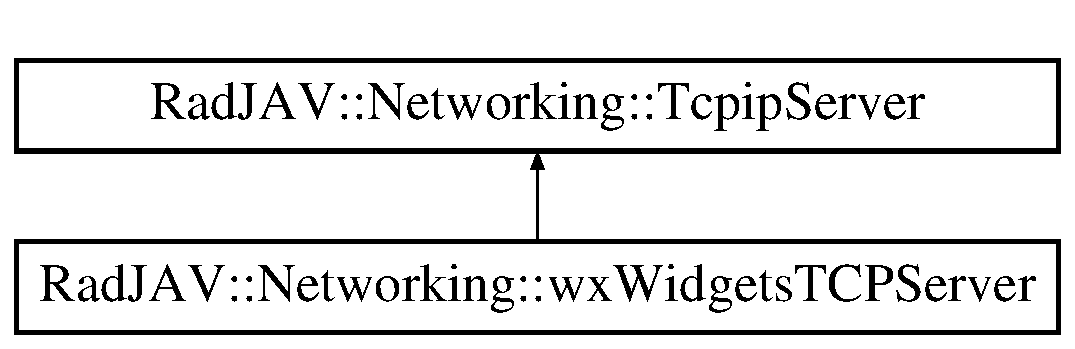
\includegraphics[height=2.000000cm]{class_rad_j_a_v_1_1_networking_1_1_tcpip_server}
\end{center}
\end{figure}
\subsection*{Public Member Functions}
\begin{DoxyCompactItemize}
\item 
\hyperlink{class_rad_j_a_v_1_1_networking_1_1_tcpip_server_ad7121698db184467e9439fe062b5d35a}{Tcpip\+Server} ()
\item 
virtual bool \hyperlink{class_rad_j_a_v_1_1_networking_1_1_tcpip_server_a3d67bcb55aae5c4cc937113c2def86b9}{init} (unsigned short new\+Port)=0
\begin{DoxyCompactList}\small\item\em Start the server. \end{DoxyCompactList}\item 
virtual bool \hyperlink{class_rad_j_a_v_1_1_networking_1_1_tcpip_server_a53555ae267a5f3d6ac8aafbb7a567ee9}{accept\+With\+Blocking} ()=0
\item 
virtual bool \hyperlink{class_rad_j_a_v_1_1_networking_1_1_tcpip_server_a3d7ea19180509cffa6d4ee802767ca90}{accept\+Without\+Blocking} ()=0
\item 
virtual bool \hyperlink{class_rad_j_a_v_1_1_networking_1_1_tcpip_server_a010c397f06fd6b6344fed2957082cc94}{send\+Float\+To\+All} (float f\+Float, std\+::vector$<$ unsigned int $>$ except=std\+::vector$<$ unsigned int $>$())=0
\item 
virtual bool \hyperlink{class_rad_j_a_v_1_1_networking_1_1_tcpip_server_af853c22dbaed2cebcfa9eb434bf0bca3}{send\+Float} (unsigned int id, float f\+Float)=0
\item 
virtual bool \hyperlink{class_rad_j_a_v_1_1_networking_1_1_tcpip_server_a898cff16cd54978e362100333e29fb50}{send\+Double\+To\+All} (double d\+Double, std\+::vector$<$ unsigned int $>$ except=std\+::vector$<$ unsigned int $>$())=0
\item 
virtual bool \hyperlink{class_rad_j_a_v_1_1_networking_1_1_tcpip_server_a0fd3de45f41e253be2228f18f244853d}{send\+Double} (unsigned int id, double d\+Double)=0
\item 
virtual bool \hyperlink{class_rad_j_a_v_1_1_networking_1_1_tcpip_server_a50b7f5fd03623836a5ee82e8389ed66f}{send\+Int\+To\+All} (int i\+Int, std\+::vector$<$ unsigned int $>$ except=std\+::vector$<$ unsigned int $>$())=0
\item 
virtual bool \hyperlink{class_rad_j_a_v_1_1_networking_1_1_tcpip_server_a815323e68b2d921e324292295a9fcb67}{send\+Int} (unsigned int id, int i\+Int)=0
\item 
virtual bool \hyperlink{class_rad_j_a_v_1_1_networking_1_1_tcpip_server_a6e60288010a4560fc00a4035e1c2a470}{send\+U\+Int\+To\+All} (unsigned int ui\+Int, std\+::vector$<$ unsigned int $>$ except=std\+::vector$<$ unsigned int $>$())=0
\item 
virtual bool \hyperlink{class_rad_j_a_v_1_1_networking_1_1_tcpip_server_a465d9c6e6611f015c566acc890f22e4e}{send\+U\+Int} (unsigned int id, unsigned int ui\+Int)=0
\item 
virtual bool \hyperlink{class_rad_j_a_v_1_1_networking_1_1_tcpip_server_a127b99aa98eb1d48001376a33190e81a}{send\+Long\+To\+All} (long l\+Long, std\+::vector$<$ unsigned int $>$ except=std\+::vector$<$ unsigned int $>$())=0
\item 
virtual bool \hyperlink{class_rad_j_a_v_1_1_networking_1_1_tcpip_server_a9daf0399b1b6cd1226221d0d8bde7993}{send\+Long} (unsigned int id, long l\+Long)=0
\item 
virtual bool \hyperlink{class_rad_j_a_v_1_1_networking_1_1_tcpip_server_ab87680c4aa41a1cd7bb7b9e56bc0e344}{send\+U\+Long\+To\+All} (unsigned long ul\+Long, std\+::vector$<$ unsigned int $>$ except=std\+::vector$<$ unsigned int $>$())=0
\item 
virtual bool \hyperlink{class_rad_j_a_v_1_1_networking_1_1_tcpip_server_aafae1fc2ff43ed3c66d721b88fc9d9b0}{send\+U\+Long} (unsigned int id, unsigned long ul\+Long)=0
\item 
virtual bool \hyperlink{class_rad_j_a_v_1_1_networking_1_1_tcpip_server_a10114a421a940cc5da3b54a10f732e30}{send\+Short\+To\+All} (short s\+Short, std\+::vector$<$ unsigned int $>$ except=std\+::vector$<$ unsigned int $>$())=0
\item 
virtual bool \hyperlink{class_rad_j_a_v_1_1_networking_1_1_tcpip_server_aaa24c728d0eb2066938c762d24927568}{send\+Short} (unsigned int id, short s\+Short)=0
\item 
virtual bool \hyperlink{class_rad_j_a_v_1_1_networking_1_1_tcpip_server_ae883e39f5bde3d790a47faa29f79b49d}{send\+U\+Short\+To\+All} (unsigned short us\+Short, std\+::vector$<$ unsigned int $>$ except=std\+::vector$<$ unsigned int $>$())=0
\item 
virtual bool \hyperlink{class_rad_j_a_v_1_1_networking_1_1_tcpip_server_a0e2f2edd1580ae9bc37667ed6f85554e}{send\+U\+Short} (unsigned int id, unsigned short us\+Short)=0
\item 
virtual bool \hyperlink{class_rad_j_a_v_1_1_networking_1_1_tcpip_server_a870b35e5674485806030587fa5e80cf7}{send\+Char\+To\+All} (char c\+Char, std\+::vector$<$ unsigned int $>$ except=std\+::vector$<$ unsigned int $>$())=0
\item 
virtual bool \hyperlink{class_rad_j_a_v_1_1_networking_1_1_tcpip_server_a2004f9c706b743af1555a487b8d5e980}{send\+Char} (unsigned int id, char c\+Char)=0
\item 
virtual bool \hyperlink{class_rad_j_a_v_1_1_networking_1_1_tcpip_server_a9dcb14e9366e92436de6c604722424f1}{send\+U\+Char\+To\+All} (unsigned char uc\+Char, std\+::vector$<$ unsigned int $>$ except=std\+::vector$<$ unsigned int $>$())=0
\item 
virtual bool \hyperlink{class_rad_j_a_v_1_1_networking_1_1_tcpip_server_a5fee9e1d19e38a5c88773d664d9b5641}{send\+U\+Char} (unsigned int id, unsigned char uc\+Char)=0
\item 
virtual bool \hyperlink{class_rad_j_a_v_1_1_networking_1_1_tcpip_server_a4259c3a04b3b0eb6ffaf175f5a779b2b}{send\+String\+To\+All} (\hyperlink{class_rad_j_a_v_1_1_string}{String} line, std\+::vector$<$ unsigned int $>$ except=std\+::vector$<$ unsigned int $>$())=0
\item 
virtual bool \hyperlink{class_rad_j_a_v_1_1_networking_1_1_tcpip_server_a009afc6e3d61e200109d39f90a692cc9}{send\+String} (unsigned int id, \hyperlink{class_rad_j_a_v_1_1_string}{String} line)=0
\item 
virtual std\+::vector$<$ \hyperlink{class_rad_j_a_v_1_1_networking_1_1_t_c_p_response}{T\+C\+P\+Response}$<$ float $>$ $>$ \hyperlink{class_rad_j_a_v_1_1_networking_1_1_tcpip_server_a99113c9c8db6b16c804c8efefd0fedae}{recv\+Float} ()=0
\begin{DoxyCompactList}\small\item\em Receive an array of floats from the connected clients. \end{DoxyCompactList}\item 
virtual std\+::vector$<$ \hyperlink{class_rad_j_a_v_1_1_networking_1_1_t_c_p_response}{T\+C\+P\+Response}$<$ double $>$ $>$ \hyperlink{class_rad_j_a_v_1_1_networking_1_1_tcpip_server_a42628f9e5e784604d970fea3fce7d5c9}{recv\+Double} ()=0
\begin{DoxyCompactList}\small\item\em Receive an array of doubles from the connected clients. \end{DoxyCompactList}\item 
virtual std\+::vector$<$ \hyperlink{class_rad_j_a_v_1_1_networking_1_1_t_c_p_response}{T\+C\+P\+Response}$<$ int $>$ $>$ \hyperlink{class_rad_j_a_v_1_1_networking_1_1_tcpip_server_a728b63e038645a7da857c1e1e628a249}{recv\+Int} ()=0
\begin{DoxyCompactList}\small\item\em Receive an array of ints from the connected clients. \end{DoxyCompactList}\item 
virtual std\+::vector$<$ \hyperlink{class_rad_j_a_v_1_1_networking_1_1_t_c_p_response}{T\+C\+P\+Response}$<$ unsigned int $>$ $>$ \hyperlink{class_rad_j_a_v_1_1_networking_1_1_tcpip_server_a05ea2d808e273d6e2cd4561df51323a7}{recv\+U\+Int} ()=0
\begin{DoxyCompactList}\small\item\em Receive an array of unsigned ints from the connected clients. \end{DoxyCompactList}\item 
virtual std\+::vector$<$ \hyperlink{class_rad_j_a_v_1_1_networking_1_1_t_c_p_response}{T\+C\+P\+Response}$<$ long $>$ $>$ \hyperlink{class_rad_j_a_v_1_1_networking_1_1_tcpip_server_aaf828d5448e9ef57b7f5c3748941fb9d}{recv\+Long} ()=0
\begin{DoxyCompactList}\small\item\em Receive an array of longs from the connected clients. \end{DoxyCompactList}\item 
virtual std\+::vector$<$ \hyperlink{class_rad_j_a_v_1_1_networking_1_1_t_c_p_response}{T\+C\+P\+Response}$<$ unsigned long $>$ $>$ \hyperlink{class_rad_j_a_v_1_1_networking_1_1_tcpip_server_abc20c6804ca546955ce5e9e4e7c3f55c}{recv\+U\+Long} ()=0
\begin{DoxyCompactList}\small\item\em Receive an array of unsigned longs from the connected clients. \end{DoxyCompactList}\item 
virtual std\+::vector$<$ \hyperlink{class_rad_j_a_v_1_1_networking_1_1_t_c_p_response}{T\+C\+P\+Response}$<$ short $>$ $>$ \hyperlink{class_rad_j_a_v_1_1_networking_1_1_tcpip_server_a398843f8da75d99ed5ff5c10b5504304}{recv\+Short} ()=0
\begin{DoxyCompactList}\small\item\em Receive an array of shorts from the connected clients. \end{DoxyCompactList}\item 
virtual std\+::vector$<$ \hyperlink{class_rad_j_a_v_1_1_networking_1_1_t_c_p_response}{T\+C\+P\+Response}$<$ unsigned short $>$ $>$ \hyperlink{class_rad_j_a_v_1_1_networking_1_1_tcpip_server_a506ef837d82be03aa3c6bb1c6b44bfc1}{recv\+U\+Short} ()=0
\begin{DoxyCompactList}\small\item\em Receive an array of unsigned shorts from the connected clients. \end{DoxyCompactList}\item 
virtual std\+::vector$<$ \hyperlink{class_rad_j_a_v_1_1_networking_1_1_t_c_p_response}{T\+C\+P\+Response}$<$ char $>$ $>$ \hyperlink{class_rad_j_a_v_1_1_networking_1_1_tcpip_server_a1e9b75bd3eccf46033d3c3b0a14c4ced}{recv\+Char} ()=0
\begin{DoxyCompactList}\small\item\em Receive an array of chars from the connected clients. \end{DoxyCompactList}\item 
virtual std\+::vector$<$ \hyperlink{class_rad_j_a_v_1_1_networking_1_1_t_c_p_response}{T\+C\+P\+Response}$<$ unsigned char $>$ $>$ \hyperlink{class_rad_j_a_v_1_1_networking_1_1_tcpip_server_ac4d92ac7eb86c234f4f46cb7c794c917}{recv\+U\+Char} ()=0
\begin{DoxyCompactList}\small\item\em Receive an array of unsigned chars from the connected clients. \end{DoxyCompactList}\item 
virtual std\+::vector$<$ \hyperlink{class_rad_j_a_v_1_1_networking_1_1_t_c_p_response}{T\+C\+P\+Response}$<$ char $\ast$ $>$ $>$ \hyperlink{class_rad_j_a_v_1_1_networking_1_1_tcpip_server_a20703e81091a1823c8d9f62c28785e48}{recv\+String} (int i\+Length)=0
\begin{DoxyCompactList}\small\item\em Receive a char array from the connected clients. \end{DoxyCompactList}\item 
virtual std\+::vector$<$ \hyperlink{class_rad_j_a_v_1_1_networking_1_1_t_c_p_response}{T\+C\+P\+Response}$<$ \hyperlink{class_rad_j_a_v_1_1_string}{String} $>$ $>$ \hyperlink{class_rad_j_a_v_1_1_networking_1_1_tcpip_server_a167e4f5fd04b01e43a00f99fd1227ce5}{recv\+String} ()=0
\begin{DoxyCompactList}\small\item\em Receive an array of strings from the connected clients. \end{DoxyCompactList}\item 
std\+::vector$<$ std\+::shared\+\_\+ptr$<$ \hyperlink{class_rad_j_a_v_1_1_networking_1_1_t_c_p_connection}{T\+C\+P\+Connection} $>$ $>$ \hyperlink{class_rad_j_a_v_1_1_networking_1_1_tcpip_server_a02492cac1eaf4ac14d2457666621fae5}{get\+Connected\+Clients} ()
\begin{DoxyCompactList}\small\item\em Get the connected clients. \end{DoxyCompactList}\item 
std\+::shared\+\_\+ptr$<$ \hyperlink{class_rad_j_a_v_1_1_networking_1_1_t_c_p_connection}{T\+C\+P\+Connection} $>$ \hyperlink{class_rad_j_a_v_1_1_networking_1_1_tcpip_server_a237daa6d6defd83bf690017edeea28ce}{get\+T\+C\+P\+Connection} (unsigned int id)
\begin{DoxyCompactList}\small\item\em Get the \hyperlink{class_rad_j_a_v_1_1_networking_1_1_t_c_p_connection}{T\+C\+P\+Connection} associated with a client id. \end{DoxyCompactList}\item 
\hyperlink{class_rad_j_a_v_1_1_string}{String} \hyperlink{class_rad_j_a_v_1_1_networking_1_1_tcpip_server_afd97d2780d61004d2a790f7f63cc4ed7}{get\+IP} (unsigned int id)
\begin{DoxyCompactList}\small\item\em Get the IP address of a connected client. \end{DoxyCompactList}\item 
std\+::shared\+\_\+ptr$<$ \hyperlink{class_rad_j_a_v_1_1_networking_1_1_t_c_p_connection}{T\+C\+P\+Connection} $>$ \hyperlink{class_rad_j_a_v_1_1_networking_1_1_tcpip_server_ab3161184633ef9072ba431ca45c408a9}{get\+Last\+T\+C\+P\+Connection} ()
\begin{DoxyCompactList}\small\item\em Get the last connected client\textquotesingle{}s \hyperlink{class_rad_j_a_v_1_1_networking_1_1_t_c_p_connection}{T\+C\+P\+Connection}. \end{DoxyCompactList}\item 
unsigned int \hyperlink{class_rad_j_a_v_1_1_networking_1_1_tcpip_server_a84eba14d877a68c241487cfc0a6d9031}{get\+Num\+Connected} ()
\begin{DoxyCompactList}\small\item\em Get the number of connected clients. \end{DoxyCompactList}\item 
unsigned short \hyperlink{class_rad_j_a_v_1_1_networking_1_1_tcpip_server_a27aecbe03f731d38e635dc1e8cbe7130}{get\+Port} ()
\begin{DoxyCompactList}\small\item\em Get the port being used. \end{DoxyCompactList}\item 
\hyperlink{class_rad_j_a_v_1_1_string}{String} \hyperlink{class_rad_j_a_v_1_1_networking_1_1_tcpip_server_a08fbc1566fc5e913bccdb1d4e392bdd5}{get\+Last\+Error} ()
\begin{DoxyCompactList}\small\item\em Get the last error thrown. \end{DoxyCompactList}\item 
std\+::vector$<$ unsigned int $>$ \hyperlink{class_rad_j_a_v_1_1_networking_1_1_tcpip_server_af5f40a952e032ff6e403e42525efe918}{get\+Last\+Received\+From\+List} ()
\item 
virtual bool \hyperlink{class_rad_j_a_v_1_1_networking_1_1_tcpip_server_a58c5ca09e1e7d121905b07eae252436c}{is\+Socket\+Open} (unsigned int id)=0
\begin{DoxyCompactList}\small\item\em Checks to see if the socket is open to a connected client. \end{DoxyCompactList}\item 
virtual bool \hyperlink{class_rad_j_a_v_1_1_networking_1_1_tcpip_server_a70d83ea527d47572c39f6e1f9a74ddd1}{close\+Client} (unsigned int id)=0
\begin{DoxyCompactList}\small\item\em Closes the connection to a connected client. \end{DoxyCompactList}\item 
virtual bool \hyperlink{class_rad_j_a_v_1_1_networking_1_1_tcpip_server_adc98bbb81534697c37b6c30662fe43dc}{close} ()=0
\begin{DoxyCompactList}\small\item\em Closes all connections with all clients and shuts down the server. \end{DoxyCompactList}\end{DoxyCompactItemize}


\subsection{Detailed Description}
Start a T\+C\+P/\+IP server. 

\subsection{Constructor \& Destructor Documentation}
\index{Rad\+J\+A\+V\+::\+Networking\+::\+Tcpip\+Server@{Rad\+J\+A\+V\+::\+Networking\+::\+Tcpip\+Server}!Tcpip\+Server@{Tcpip\+Server}}
\index{Tcpip\+Server@{Tcpip\+Server}!Rad\+J\+A\+V\+::\+Networking\+::\+Tcpip\+Server@{Rad\+J\+A\+V\+::\+Networking\+::\+Tcpip\+Server}}
\subsubsection[{\texorpdfstring{Tcpip\+Server()}{TcpipServer()}}]{\setlength{\rightskip}{0pt plus 5cm}Rad\+J\+A\+V\+::\+Networking\+::\+Tcpip\+Server\+::\+Tcpip\+Server (
\begin{DoxyParamCaption}
{}
\end{DoxyParamCaption}
)}\hypertarget{class_rad_j_a_v_1_1_networking_1_1_tcpip_server_ad7121698db184467e9439fe062b5d35a}{}\label{class_rad_j_a_v_1_1_networking_1_1_tcpip_server_ad7121698db184467e9439fe062b5d35a}


\subsection{Member Function Documentation}
\index{Rad\+J\+A\+V\+::\+Networking\+::\+Tcpip\+Server@{Rad\+J\+A\+V\+::\+Networking\+::\+Tcpip\+Server}!accept\+With\+Blocking@{accept\+With\+Blocking}}
\index{accept\+With\+Blocking@{accept\+With\+Blocking}!Rad\+J\+A\+V\+::\+Networking\+::\+Tcpip\+Server@{Rad\+J\+A\+V\+::\+Networking\+::\+Tcpip\+Server}}
\subsubsection[{\texorpdfstring{accept\+With\+Blocking()=0}{acceptWithBlocking()=0}}]{\setlength{\rightskip}{0pt plus 5cm}virtual bool Rad\+J\+A\+V\+::\+Networking\+::\+Tcpip\+Server\+::accept\+With\+Blocking (
\begin{DoxyParamCaption}
{}
\end{DoxyParamCaption}
)\hspace{0.3cm}{\ttfamily [pure virtual]}}\hypertarget{class_rad_j_a_v_1_1_networking_1_1_tcpip_server_a53555ae267a5f3d6ac8aafbb7a567ee9}{}\label{class_rad_j_a_v_1_1_networking_1_1_tcpip_server_a53555ae267a5f3d6ac8aafbb7a567ee9}
Listen for connections and lock the current thread. 

Implemented in \hyperlink{class_rad_j_a_v_1_1_networking_1_1wx_widgets_t_c_p_server_a09b2a943dc69cab1aa3bf1573a8f72c1}{Rad\+J\+A\+V\+::\+Networking\+::wx\+Widgets\+T\+C\+P\+Server}.

\index{Rad\+J\+A\+V\+::\+Networking\+::\+Tcpip\+Server@{Rad\+J\+A\+V\+::\+Networking\+::\+Tcpip\+Server}!accept\+Without\+Blocking@{accept\+Without\+Blocking}}
\index{accept\+Without\+Blocking@{accept\+Without\+Blocking}!Rad\+J\+A\+V\+::\+Networking\+::\+Tcpip\+Server@{Rad\+J\+A\+V\+::\+Networking\+::\+Tcpip\+Server}}
\subsubsection[{\texorpdfstring{accept\+Without\+Blocking()=0}{acceptWithoutBlocking()=0}}]{\setlength{\rightskip}{0pt plus 5cm}virtual bool Rad\+J\+A\+V\+::\+Networking\+::\+Tcpip\+Server\+::accept\+Without\+Blocking (
\begin{DoxyParamCaption}
{}
\end{DoxyParamCaption}
)\hspace{0.3cm}{\ttfamily [pure virtual]}}\hypertarget{class_rad_j_a_v_1_1_networking_1_1_tcpip_server_a3d7ea19180509cffa6d4ee802767ca90}{}\label{class_rad_j_a_v_1_1_networking_1_1_tcpip_server_a3d7ea19180509cffa6d4ee802767ca90}
Listen for connections and do not lock the current thread. 

Implemented in \hyperlink{class_rad_j_a_v_1_1_networking_1_1wx_widgets_t_c_p_server_a1e78417fa012bebbc21fbcf8557c8008}{Rad\+J\+A\+V\+::\+Networking\+::wx\+Widgets\+T\+C\+P\+Server}.

\index{Rad\+J\+A\+V\+::\+Networking\+::\+Tcpip\+Server@{Rad\+J\+A\+V\+::\+Networking\+::\+Tcpip\+Server}!close@{close}}
\index{close@{close}!Rad\+J\+A\+V\+::\+Networking\+::\+Tcpip\+Server@{Rad\+J\+A\+V\+::\+Networking\+::\+Tcpip\+Server}}
\subsubsection[{\texorpdfstring{close()=0}{close()=0}}]{\setlength{\rightskip}{0pt plus 5cm}virtual bool Rad\+J\+A\+V\+::\+Networking\+::\+Tcpip\+Server\+::close (
\begin{DoxyParamCaption}
{}
\end{DoxyParamCaption}
)\hspace{0.3cm}{\ttfamily [pure virtual]}}\hypertarget{class_rad_j_a_v_1_1_networking_1_1_tcpip_server_adc98bbb81534697c37b6c30662fe43dc}{}\label{class_rad_j_a_v_1_1_networking_1_1_tcpip_server_adc98bbb81534697c37b6c30662fe43dc}


Closes all connections with all clients and shuts down the server. 

\index{Rad\+J\+A\+V\+::\+Networking\+::\+Tcpip\+Server@{Rad\+J\+A\+V\+::\+Networking\+::\+Tcpip\+Server}!close\+Client@{close\+Client}}
\index{close\+Client@{close\+Client}!Rad\+J\+A\+V\+::\+Networking\+::\+Tcpip\+Server@{Rad\+J\+A\+V\+::\+Networking\+::\+Tcpip\+Server}}
\subsubsection[{\texorpdfstring{close\+Client(unsigned int id)=0}{closeClient(unsigned int id)=0}}]{\setlength{\rightskip}{0pt plus 5cm}virtual bool Rad\+J\+A\+V\+::\+Networking\+::\+Tcpip\+Server\+::close\+Client (
\begin{DoxyParamCaption}
\item[{unsigned int}]{id}
\end{DoxyParamCaption}
)\hspace{0.3cm}{\ttfamily [pure virtual]}}\hypertarget{class_rad_j_a_v_1_1_networking_1_1_tcpip_server_a70d83ea527d47572c39f6e1f9a74ddd1}{}\label{class_rad_j_a_v_1_1_networking_1_1_tcpip_server_a70d83ea527d47572c39f6e1f9a74ddd1}


Closes the connection to a connected client. 

\index{Rad\+J\+A\+V\+::\+Networking\+::\+Tcpip\+Server@{Rad\+J\+A\+V\+::\+Networking\+::\+Tcpip\+Server}!get\+Connected\+Clients@{get\+Connected\+Clients}}
\index{get\+Connected\+Clients@{get\+Connected\+Clients}!Rad\+J\+A\+V\+::\+Networking\+::\+Tcpip\+Server@{Rad\+J\+A\+V\+::\+Networking\+::\+Tcpip\+Server}}
\subsubsection[{\texorpdfstring{get\+Connected\+Clients()}{getConnectedClients()}}]{\setlength{\rightskip}{0pt plus 5cm}std\+::vector$<$ std\+::shared\+\_\+ptr$<$ {\bf T\+C\+P\+Connection} $>$ $>$ Rad\+J\+A\+V\+::\+Networking\+::\+Tcpip\+Server\+::get\+Connected\+Clients (
\begin{DoxyParamCaption}
{}
\end{DoxyParamCaption}
)}\hypertarget{class_rad_j_a_v_1_1_networking_1_1_tcpip_server_a02492cac1eaf4ac14d2457666621fae5}{}\label{class_rad_j_a_v_1_1_networking_1_1_tcpip_server_a02492cac1eaf4ac14d2457666621fae5}


Get the connected clients. 

\index{Rad\+J\+A\+V\+::\+Networking\+::\+Tcpip\+Server@{Rad\+J\+A\+V\+::\+Networking\+::\+Tcpip\+Server}!get\+IP@{get\+IP}}
\index{get\+IP@{get\+IP}!Rad\+J\+A\+V\+::\+Networking\+::\+Tcpip\+Server@{Rad\+J\+A\+V\+::\+Networking\+::\+Tcpip\+Server}}
\subsubsection[{\texorpdfstring{get\+I\+P(unsigned int id)}{getIP(unsigned int id)}}]{\setlength{\rightskip}{0pt plus 5cm}{\bf String} Rad\+J\+A\+V\+::\+Networking\+::\+Tcpip\+Server\+::get\+IP (
\begin{DoxyParamCaption}
\item[{unsigned int}]{id}
\end{DoxyParamCaption}
)}\hypertarget{class_rad_j_a_v_1_1_networking_1_1_tcpip_server_afd97d2780d61004d2a790f7f63cc4ed7}{}\label{class_rad_j_a_v_1_1_networking_1_1_tcpip_server_afd97d2780d61004d2a790f7f63cc4ed7}


Get the IP address of a connected client. 

\index{Rad\+J\+A\+V\+::\+Networking\+::\+Tcpip\+Server@{Rad\+J\+A\+V\+::\+Networking\+::\+Tcpip\+Server}!get\+Last\+Error@{get\+Last\+Error}}
\index{get\+Last\+Error@{get\+Last\+Error}!Rad\+J\+A\+V\+::\+Networking\+::\+Tcpip\+Server@{Rad\+J\+A\+V\+::\+Networking\+::\+Tcpip\+Server}}
\subsubsection[{\texorpdfstring{get\+Last\+Error()}{getLastError()}}]{\setlength{\rightskip}{0pt plus 5cm}{\bf String} Rad\+J\+A\+V\+::\+Networking\+::\+Tcpip\+Server\+::get\+Last\+Error (
\begin{DoxyParamCaption}
{}
\end{DoxyParamCaption}
)}\hypertarget{class_rad_j_a_v_1_1_networking_1_1_tcpip_server_a08fbc1566fc5e913bccdb1d4e392bdd5}{}\label{class_rad_j_a_v_1_1_networking_1_1_tcpip_server_a08fbc1566fc5e913bccdb1d4e392bdd5}


Get the last error thrown. 

\index{Rad\+J\+A\+V\+::\+Networking\+::\+Tcpip\+Server@{Rad\+J\+A\+V\+::\+Networking\+::\+Tcpip\+Server}!get\+Last\+Received\+From\+List@{get\+Last\+Received\+From\+List}}
\index{get\+Last\+Received\+From\+List@{get\+Last\+Received\+From\+List}!Rad\+J\+A\+V\+::\+Networking\+::\+Tcpip\+Server@{Rad\+J\+A\+V\+::\+Networking\+::\+Tcpip\+Server}}
\subsubsection[{\texorpdfstring{get\+Last\+Received\+From\+List()}{getLastReceivedFromList()}}]{\setlength{\rightskip}{0pt plus 5cm}std\+::vector$<$ unsigned int $>$ Rad\+J\+A\+V\+::\+Networking\+::\+Tcpip\+Server\+::get\+Last\+Received\+From\+List (
\begin{DoxyParamCaption}
{}
\end{DoxyParamCaption}
)}\hypertarget{class_rad_j_a_v_1_1_networking_1_1_tcpip_server_af5f40a952e032ff6e403e42525efe918}{}\label{class_rad_j_a_v_1_1_networking_1_1_tcpip_server_af5f40a952e032ff6e403e42525efe918}
\index{Rad\+J\+A\+V\+::\+Networking\+::\+Tcpip\+Server@{Rad\+J\+A\+V\+::\+Networking\+::\+Tcpip\+Server}!get\+Last\+T\+C\+P\+Connection@{get\+Last\+T\+C\+P\+Connection}}
\index{get\+Last\+T\+C\+P\+Connection@{get\+Last\+T\+C\+P\+Connection}!Rad\+J\+A\+V\+::\+Networking\+::\+Tcpip\+Server@{Rad\+J\+A\+V\+::\+Networking\+::\+Tcpip\+Server}}
\subsubsection[{\texorpdfstring{get\+Last\+T\+C\+P\+Connection()}{getLastTCPConnection()}}]{\setlength{\rightskip}{0pt plus 5cm}std\+::shared\+\_\+ptr$<$ {\bf T\+C\+P\+Connection} $>$ Rad\+J\+A\+V\+::\+Networking\+::\+Tcpip\+Server\+::get\+Last\+T\+C\+P\+Connection (
\begin{DoxyParamCaption}
{}
\end{DoxyParamCaption}
)}\hypertarget{class_rad_j_a_v_1_1_networking_1_1_tcpip_server_ab3161184633ef9072ba431ca45c408a9}{}\label{class_rad_j_a_v_1_1_networking_1_1_tcpip_server_ab3161184633ef9072ba431ca45c408a9}


Get the last connected client\textquotesingle{}s \hyperlink{class_rad_j_a_v_1_1_networking_1_1_t_c_p_connection}{T\+C\+P\+Connection}. 

\index{Rad\+J\+A\+V\+::\+Networking\+::\+Tcpip\+Server@{Rad\+J\+A\+V\+::\+Networking\+::\+Tcpip\+Server}!get\+Num\+Connected@{get\+Num\+Connected}}
\index{get\+Num\+Connected@{get\+Num\+Connected}!Rad\+J\+A\+V\+::\+Networking\+::\+Tcpip\+Server@{Rad\+J\+A\+V\+::\+Networking\+::\+Tcpip\+Server}}
\subsubsection[{\texorpdfstring{get\+Num\+Connected()}{getNumConnected()}}]{\setlength{\rightskip}{0pt plus 5cm}unsigned int Rad\+J\+A\+V\+::\+Networking\+::\+Tcpip\+Server\+::get\+Num\+Connected (
\begin{DoxyParamCaption}
{}
\end{DoxyParamCaption}
)}\hypertarget{class_rad_j_a_v_1_1_networking_1_1_tcpip_server_a84eba14d877a68c241487cfc0a6d9031}{}\label{class_rad_j_a_v_1_1_networking_1_1_tcpip_server_a84eba14d877a68c241487cfc0a6d9031}


Get the number of connected clients. 

\index{Rad\+J\+A\+V\+::\+Networking\+::\+Tcpip\+Server@{Rad\+J\+A\+V\+::\+Networking\+::\+Tcpip\+Server}!get\+Port@{get\+Port}}
\index{get\+Port@{get\+Port}!Rad\+J\+A\+V\+::\+Networking\+::\+Tcpip\+Server@{Rad\+J\+A\+V\+::\+Networking\+::\+Tcpip\+Server}}
\subsubsection[{\texorpdfstring{get\+Port()}{getPort()}}]{\setlength{\rightskip}{0pt plus 5cm}unsigned short Rad\+J\+A\+V\+::\+Networking\+::\+Tcpip\+Server\+::get\+Port (
\begin{DoxyParamCaption}
{}
\end{DoxyParamCaption}
)}\hypertarget{class_rad_j_a_v_1_1_networking_1_1_tcpip_server_a27aecbe03f731d38e635dc1e8cbe7130}{}\label{class_rad_j_a_v_1_1_networking_1_1_tcpip_server_a27aecbe03f731d38e635dc1e8cbe7130}


Get the port being used. 

\index{Rad\+J\+A\+V\+::\+Networking\+::\+Tcpip\+Server@{Rad\+J\+A\+V\+::\+Networking\+::\+Tcpip\+Server}!get\+T\+C\+P\+Connection@{get\+T\+C\+P\+Connection}}
\index{get\+T\+C\+P\+Connection@{get\+T\+C\+P\+Connection}!Rad\+J\+A\+V\+::\+Networking\+::\+Tcpip\+Server@{Rad\+J\+A\+V\+::\+Networking\+::\+Tcpip\+Server}}
\subsubsection[{\texorpdfstring{get\+T\+C\+P\+Connection(unsigned int id)}{getTCPConnection(unsigned int id)}}]{\setlength{\rightskip}{0pt plus 5cm}std\+::shared\+\_\+ptr$<$ {\bf T\+C\+P\+Connection} $>$ Rad\+J\+A\+V\+::\+Networking\+::\+Tcpip\+Server\+::get\+T\+C\+P\+Connection (
\begin{DoxyParamCaption}
\item[{unsigned int}]{id}
\end{DoxyParamCaption}
)}\hypertarget{class_rad_j_a_v_1_1_networking_1_1_tcpip_server_a237daa6d6defd83bf690017edeea28ce}{}\label{class_rad_j_a_v_1_1_networking_1_1_tcpip_server_a237daa6d6defd83bf690017edeea28ce}


Get the \hyperlink{class_rad_j_a_v_1_1_networking_1_1_t_c_p_connection}{T\+C\+P\+Connection} associated with a client id. 

\index{Rad\+J\+A\+V\+::\+Networking\+::\+Tcpip\+Server@{Rad\+J\+A\+V\+::\+Networking\+::\+Tcpip\+Server}!init@{init}}
\index{init@{init}!Rad\+J\+A\+V\+::\+Networking\+::\+Tcpip\+Server@{Rad\+J\+A\+V\+::\+Networking\+::\+Tcpip\+Server}}
\subsubsection[{\texorpdfstring{init(unsigned short new\+Port)=0}{init(unsigned short newPort)=0}}]{\setlength{\rightskip}{0pt plus 5cm}virtual bool Rad\+J\+A\+V\+::\+Networking\+::\+Tcpip\+Server\+::init (
\begin{DoxyParamCaption}
\item[{unsigned short}]{new\+Port}
\end{DoxyParamCaption}
)\hspace{0.3cm}{\ttfamily [pure virtual]}}\hypertarget{class_rad_j_a_v_1_1_networking_1_1_tcpip_server_a3d67bcb55aae5c4cc937113c2def86b9}{}\label{class_rad_j_a_v_1_1_networking_1_1_tcpip_server_a3d67bcb55aae5c4cc937113c2def86b9}


Start the server. 



Implemented in \hyperlink{class_rad_j_a_v_1_1_networking_1_1wx_widgets_t_c_p_server_aa0c34e3462f10c401629f9cea3a113a4}{Rad\+J\+A\+V\+::\+Networking\+::wx\+Widgets\+T\+C\+P\+Server}.

\index{Rad\+J\+A\+V\+::\+Networking\+::\+Tcpip\+Server@{Rad\+J\+A\+V\+::\+Networking\+::\+Tcpip\+Server}!is\+Socket\+Open@{is\+Socket\+Open}}
\index{is\+Socket\+Open@{is\+Socket\+Open}!Rad\+J\+A\+V\+::\+Networking\+::\+Tcpip\+Server@{Rad\+J\+A\+V\+::\+Networking\+::\+Tcpip\+Server}}
\subsubsection[{\texorpdfstring{is\+Socket\+Open(unsigned int id)=0}{isSocketOpen(unsigned int id)=0}}]{\setlength{\rightskip}{0pt plus 5cm}virtual bool Rad\+J\+A\+V\+::\+Networking\+::\+Tcpip\+Server\+::is\+Socket\+Open (
\begin{DoxyParamCaption}
\item[{unsigned int}]{id}
\end{DoxyParamCaption}
)\hspace{0.3cm}{\ttfamily [pure virtual]}}\hypertarget{class_rad_j_a_v_1_1_networking_1_1_tcpip_server_a58c5ca09e1e7d121905b07eae252436c}{}\label{class_rad_j_a_v_1_1_networking_1_1_tcpip_server_a58c5ca09e1e7d121905b07eae252436c}


Checks to see if the socket is open to a connected client. 

\index{Rad\+J\+A\+V\+::\+Networking\+::\+Tcpip\+Server@{Rad\+J\+A\+V\+::\+Networking\+::\+Tcpip\+Server}!recv\+Char@{recv\+Char}}
\index{recv\+Char@{recv\+Char}!Rad\+J\+A\+V\+::\+Networking\+::\+Tcpip\+Server@{Rad\+J\+A\+V\+::\+Networking\+::\+Tcpip\+Server}}
\subsubsection[{\texorpdfstring{recv\+Char()=0}{recvChar()=0}}]{\setlength{\rightskip}{0pt plus 5cm}virtual std\+::vector$<$ {\bf T\+C\+P\+Response}$<$char$>$ $>$ Rad\+J\+A\+V\+::\+Networking\+::\+Tcpip\+Server\+::recv\+Char (
\begin{DoxyParamCaption}
{}
\end{DoxyParamCaption}
)\hspace{0.3cm}{\ttfamily [pure virtual]}}\hypertarget{class_rad_j_a_v_1_1_networking_1_1_tcpip_server_a1e9b75bd3eccf46033d3c3b0a14c4ced}{}\label{class_rad_j_a_v_1_1_networking_1_1_tcpip_server_a1e9b75bd3eccf46033d3c3b0a14c4ced}


Receive an array of chars from the connected clients. 



Implemented in \hyperlink{class_rad_j_a_v_1_1_networking_1_1wx_widgets_t_c_p_server_ae964ef6ac1547ac313d8ab580ae3f7b4}{Rad\+J\+A\+V\+::\+Networking\+::wx\+Widgets\+T\+C\+P\+Server}.

\index{Rad\+J\+A\+V\+::\+Networking\+::\+Tcpip\+Server@{Rad\+J\+A\+V\+::\+Networking\+::\+Tcpip\+Server}!recv\+Double@{recv\+Double}}
\index{recv\+Double@{recv\+Double}!Rad\+J\+A\+V\+::\+Networking\+::\+Tcpip\+Server@{Rad\+J\+A\+V\+::\+Networking\+::\+Tcpip\+Server}}
\subsubsection[{\texorpdfstring{recv\+Double()=0}{recvDouble()=0}}]{\setlength{\rightskip}{0pt plus 5cm}virtual std\+::vector$<$ {\bf T\+C\+P\+Response}$<$double$>$ $>$ Rad\+J\+A\+V\+::\+Networking\+::\+Tcpip\+Server\+::recv\+Double (
\begin{DoxyParamCaption}
{}
\end{DoxyParamCaption}
)\hspace{0.3cm}{\ttfamily [pure virtual]}}\hypertarget{class_rad_j_a_v_1_1_networking_1_1_tcpip_server_a42628f9e5e784604d970fea3fce7d5c9}{}\label{class_rad_j_a_v_1_1_networking_1_1_tcpip_server_a42628f9e5e784604d970fea3fce7d5c9}


Receive an array of doubles from the connected clients. 



Implemented in \hyperlink{class_rad_j_a_v_1_1_networking_1_1wx_widgets_t_c_p_server_a1c445d2b459e6a249ec132da08f230bd}{Rad\+J\+A\+V\+::\+Networking\+::wx\+Widgets\+T\+C\+P\+Server}.

\index{Rad\+J\+A\+V\+::\+Networking\+::\+Tcpip\+Server@{Rad\+J\+A\+V\+::\+Networking\+::\+Tcpip\+Server}!recv\+Float@{recv\+Float}}
\index{recv\+Float@{recv\+Float}!Rad\+J\+A\+V\+::\+Networking\+::\+Tcpip\+Server@{Rad\+J\+A\+V\+::\+Networking\+::\+Tcpip\+Server}}
\subsubsection[{\texorpdfstring{recv\+Float()=0}{recvFloat()=0}}]{\setlength{\rightskip}{0pt plus 5cm}virtual std\+::vector$<$ {\bf T\+C\+P\+Response}$<$float$>$ $>$ Rad\+J\+A\+V\+::\+Networking\+::\+Tcpip\+Server\+::recv\+Float (
\begin{DoxyParamCaption}
{}
\end{DoxyParamCaption}
)\hspace{0.3cm}{\ttfamily [pure virtual]}}\hypertarget{class_rad_j_a_v_1_1_networking_1_1_tcpip_server_a99113c9c8db6b16c804c8efefd0fedae}{}\label{class_rad_j_a_v_1_1_networking_1_1_tcpip_server_a99113c9c8db6b16c804c8efefd0fedae}


Receive an array of floats from the connected clients. 



Implemented in \hyperlink{class_rad_j_a_v_1_1_networking_1_1wx_widgets_t_c_p_server_a25f1060df172b7ac485c062d5598ee04}{Rad\+J\+A\+V\+::\+Networking\+::wx\+Widgets\+T\+C\+P\+Server}.

\index{Rad\+J\+A\+V\+::\+Networking\+::\+Tcpip\+Server@{Rad\+J\+A\+V\+::\+Networking\+::\+Tcpip\+Server}!recv\+Int@{recv\+Int}}
\index{recv\+Int@{recv\+Int}!Rad\+J\+A\+V\+::\+Networking\+::\+Tcpip\+Server@{Rad\+J\+A\+V\+::\+Networking\+::\+Tcpip\+Server}}
\subsubsection[{\texorpdfstring{recv\+Int()=0}{recvInt()=0}}]{\setlength{\rightskip}{0pt plus 5cm}virtual std\+::vector$<$ {\bf T\+C\+P\+Response}$<$int$>$ $>$ Rad\+J\+A\+V\+::\+Networking\+::\+Tcpip\+Server\+::recv\+Int (
\begin{DoxyParamCaption}
{}
\end{DoxyParamCaption}
)\hspace{0.3cm}{\ttfamily [pure virtual]}}\hypertarget{class_rad_j_a_v_1_1_networking_1_1_tcpip_server_a728b63e038645a7da857c1e1e628a249}{}\label{class_rad_j_a_v_1_1_networking_1_1_tcpip_server_a728b63e038645a7da857c1e1e628a249}


Receive an array of ints from the connected clients. 



Implemented in \hyperlink{class_rad_j_a_v_1_1_networking_1_1wx_widgets_t_c_p_server_a141060e567ebda7607cf74fe086a8e4c}{Rad\+J\+A\+V\+::\+Networking\+::wx\+Widgets\+T\+C\+P\+Server}.

\index{Rad\+J\+A\+V\+::\+Networking\+::\+Tcpip\+Server@{Rad\+J\+A\+V\+::\+Networking\+::\+Tcpip\+Server}!recv\+Long@{recv\+Long}}
\index{recv\+Long@{recv\+Long}!Rad\+J\+A\+V\+::\+Networking\+::\+Tcpip\+Server@{Rad\+J\+A\+V\+::\+Networking\+::\+Tcpip\+Server}}
\subsubsection[{\texorpdfstring{recv\+Long()=0}{recvLong()=0}}]{\setlength{\rightskip}{0pt plus 5cm}virtual std\+::vector$<$ {\bf T\+C\+P\+Response}$<$long$>$ $>$ Rad\+J\+A\+V\+::\+Networking\+::\+Tcpip\+Server\+::recv\+Long (
\begin{DoxyParamCaption}
{}
\end{DoxyParamCaption}
)\hspace{0.3cm}{\ttfamily [pure virtual]}}\hypertarget{class_rad_j_a_v_1_1_networking_1_1_tcpip_server_aaf828d5448e9ef57b7f5c3748941fb9d}{}\label{class_rad_j_a_v_1_1_networking_1_1_tcpip_server_aaf828d5448e9ef57b7f5c3748941fb9d}


Receive an array of longs from the connected clients. 



Implemented in \hyperlink{class_rad_j_a_v_1_1_networking_1_1wx_widgets_t_c_p_server_aa52be52a0a3aaec2402f838ce39d734d}{Rad\+J\+A\+V\+::\+Networking\+::wx\+Widgets\+T\+C\+P\+Server}.

\index{Rad\+J\+A\+V\+::\+Networking\+::\+Tcpip\+Server@{Rad\+J\+A\+V\+::\+Networking\+::\+Tcpip\+Server}!recv\+Short@{recv\+Short}}
\index{recv\+Short@{recv\+Short}!Rad\+J\+A\+V\+::\+Networking\+::\+Tcpip\+Server@{Rad\+J\+A\+V\+::\+Networking\+::\+Tcpip\+Server}}
\subsubsection[{\texorpdfstring{recv\+Short()=0}{recvShort()=0}}]{\setlength{\rightskip}{0pt plus 5cm}virtual std\+::vector$<$ {\bf T\+C\+P\+Response}$<$short$>$ $>$ Rad\+J\+A\+V\+::\+Networking\+::\+Tcpip\+Server\+::recv\+Short (
\begin{DoxyParamCaption}
{}
\end{DoxyParamCaption}
)\hspace{0.3cm}{\ttfamily [pure virtual]}}\hypertarget{class_rad_j_a_v_1_1_networking_1_1_tcpip_server_a398843f8da75d99ed5ff5c10b5504304}{}\label{class_rad_j_a_v_1_1_networking_1_1_tcpip_server_a398843f8da75d99ed5ff5c10b5504304}


Receive an array of shorts from the connected clients. 



Implemented in \hyperlink{class_rad_j_a_v_1_1_networking_1_1wx_widgets_t_c_p_server_a28d61fa54cb79db09a4877832e3488ed}{Rad\+J\+A\+V\+::\+Networking\+::wx\+Widgets\+T\+C\+P\+Server}.

\index{Rad\+J\+A\+V\+::\+Networking\+::\+Tcpip\+Server@{Rad\+J\+A\+V\+::\+Networking\+::\+Tcpip\+Server}!recv\+String@{recv\+String}}
\index{recv\+String@{recv\+String}!Rad\+J\+A\+V\+::\+Networking\+::\+Tcpip\+Server@{Rad\+J\+A\+V\+::\+Networking\+::\+Tcpip\+Server}}
\subsubsection[{\texorpdfstring{recv\+String(int i\+Length)=0}{recvString(int iLength)=0}}]{\setlength{\rightskip}{0pt plus 5cm}virtual std\+::vector$<$ {\bf T\+C\+P\+Response}$<$char $\ast$$>$ $>$ Rad\+J\+A\+V\+::\+Networking\+::\+Tcpip\+Server\+::recv\+String (
\begin{DoxyParamCaption}
\item[{int}]{i\+Length}
\end{DoxyParamCaption}
)\hspace{0.3cm}{\ttfamily [pure virtual]}}\hypertarget{class_rad_j_a_v_1_1_networking_1_1_tcpip_server_a20703e81091a1823c8d9f62c28785e48}{}\label{class_rad_j_a_v_1_1_networking_1_1_tcpip_server_a20703e81091a1823c8d9f62c28785e48}


Receive a char array from the connected clients. 



Implemented in \hyperlink{class_rad_j_a_v_1_1_networking_1_1wx_widgets_t_c_p_server_a6b3ea7891f3111f89cd1610a9b1db15d}{Rad\+J\+A\+V\+::\+Networking\+::wx\+Widgets\+T\+C\+P\+Server}.

\index{Rad\+J\+A\+V\+::\+Networking\+::\+Tcpip\+Server@{Rad\+J\+A\+V\+::\+Networking\+::\+Tcpip\+Server}!recv\+String@{recv\+String}}
\index{recv\+String@{recv\+String}!Rad\+J\+A\+V\+::\+Networking\+::\+Tcpip\+Server@{Rad\+J\+A\+V\+::\+Networking\+::\+Tcpip\+Server}}
\subsubsection[{\texorpdfstring{recv\+String()=0}{recvString()=0}}]{\setlength{\rightskip}{0pt plus 5cm}virtual std\+::vector$<$ {\bf T\+C\+P\+Response}$<${\bf String}$>$ $>$ Rad\+J\+A\+V\+::\+Networking\+::\+Tcpip\+Server\+::recv\+String (
\begin{DoxyParamCaption}
{}
\end{DoxyParamCaption}
)\hspace{0.3cm}{\ttfamily [pure virtual]}}\hypertarget{class_rad_j_a_v_1_1_networking_1_1_tcpip_server_a167e4f5fd04b01e43a00f99fd1227ce5}{}\label{class_rad_j_a_v_1_1_networking_1_1_tcpip_server_a167e4f5fd04b01e43a00f99fd1227ce5}


Receive an array of strings from the connected clients. 



Implemented in \hyperlink{class_rad_j_a_v_1_1_networking_1_1wx_widgets_t_c_p_server_ac33b6977b1d527476c8f95eb91464fd9}{Rad\+J\+A\+V\+::\+Networking\+::wx\+Widgets\+T\+C\+P\+Server}.

\index{Rad\+J\+A\+V\+::\+Networking\+::\+Tcpip\+Server@{Rad\+J\+A\+V\+::\+Networking\+::\+Tcpip\+Server}!recv\+U\+Char@{recv\+U\+Char}}
\index{recv\+U\+Char@{recv\+U\+Char}!Rad\+J\+A\+V\+::\+Networking\+::\+Tcpip\+Server@{Rad\+J\+A\+V\+::\+Networking\+::\+Tcpip\+Server}}
\subsubsection[{\texorpdfstring{recv\+U\+Char()=0}{recvUChar()=0}}]{\setlength{\rightskip}{0pt plus 5cm}virtual std\+::vector$<$ {\bf T\+C\+P\+Response}$<$unsigned char$>$ $>$ Rad\+J\+A\+V\+::\+Networking\+::\+Tcpip\+Server\+::recv\+U\+Char (
\begin{DoxyParamCaption}
{}
\end{DoxyParamCaption}
)\hspace{0.3cm}{\ttfamily [pure virtual]}}\hypertarget{class_rad_j_a_v_1_1_networking_1_1_tcpip_server_ac4d92ac7eb86c234f4f46cb7c794c917}{}\label{class_rad_j_a_v_1_1_networking_1_1_tcpip_server_ac4d92ac7eb86c234f4f46cb7c794c917}


Receive an array of unsigned chars from the connected clients. 



Implemented in \hyperlink{class_rad_j_a_v_1_1_networking_1_1wx_widgets_t_c_p_server_ab4f0c794a4711e14b805f0ffde01160c}{Rad\+J\+A\+V\+::\+Networking\+::wx\+Widgets\+T\+C\+P\+Server}.

\index{Rad\+J\+A\+V\+::\+Networking\+::\+Tcpip\+Server@{Rad\+J\+A\+V\+::\+Networking\+::\+Tcpip\+Server}!recv\+U\+Int@{recv\+U\+Int}}
\index{recv\+U\+Int@{recv\+U\+Int}!Rad\+J\+A\+V\+::\+Networking\+::\+Tcpip\+Server@{Rad\+J\+A\+V\+::\+Networking\+::\+Tcpip\+Server}}
\subsubsection[{\texorpdfstring{recv\+U\+Int()=0}{recvUInt()=0}}]{\setlength{\rightskip}{0pt plus 5cm}virtual std\+::vector$<$ {\bf T\+C\+P\+Response}$<$unsigned int$>$ $>$ Rad\+J\+A\+V\+::\+Networking\+::\+Tcpip\+Server\+::recv\+U\+Int (
\begin{DoxyParamCaption}
{}
\end{DoxyParamCaption}
)\hspace{0.3cm}{\ttfamily [pure virtual]}}\hypertarget{class_rad_j_a_v_1_1_networking_1_1_tcpip_server_a05ea2d808e273d6e2cd4561df51323a7}{}\label{class_rad_j_a_v_1_1_networking_1_1_tcpip_server_a05ea2d808e273d6e2cd4561df51323a7}


Receive an array of unsigned ints from the connected clients. 



Implemented in \hyperlink{class_rad_j_a_v_1_1_networking_1_1wx_widgets_t_c_p_server_aefa435e65eef2200e74f1fd903447071}{Rad\+J\+A\+V\+::\+Networking\+::wx\+Widgets\+T\+C\+P\+Server}.

\index{Rad\+J\+A\+V\+::\+Networking\+::\+Tcpip\+Server@{Rad\+J\+A\+V\+::\+Networking\+::\+Tcpip\+Server}!recv\+U\+Long@{recv\+U\+Long}}
\index{recv\+U\+Long@{recv\+U\+Long}!Rad\+J\+A\+V\+::\+Networking\+::\+Tcpip\+Server@{Rad\+J\+A\+V\+::\+Networking\+::\+Tcpip\+Server}}
\subsubsection[{\texorpdfstring{recv\+U\+Long()=0}{recvULong()=0}}]{\setlength{\rightskip}{0pt plus 5cm}virtual std\+::vector$<$ {\bf T\+C\+P\+Response}$<$unsigned long$>$ $>$ Rad\+J\+A\+V\+::\+Networking\+::\+Tcpip\+Server\+::recv\+U\+Long (
\begin{DoxyParamCaption}
{}
\end{DoxyParamCaption}
)\hspace{0.3cm}{\ttfamily [pure virtual]}}\hypertarget{class_rad_j_a_v_1_1_networking_1_1_tcpip_server_abc20c6804ca546955ce5e9e4e7c3f55c}{}\label{class_rad_j_a_v_1_1_networking_1_1_tcpip_server_abc20c6804ca546955ce5e9e4e7c3f55c}


Receive an array of unsigned longs from the connected clients. 



Implemented in \hyperlink{class_rad_j_a_v_1_1_networking_1_1wx_widgets_t_c_p_server_a9330de8d1fe3d184006cbcfb3c88e87f}{Rad\+J\+A\+V\+::\+Networking\+::wx\+Widgets\+T\+C\+P\+Server}.

\index{Rad\+J\+A\+V\+::\+Networking\+::\+Tcpip\+Server@{Rad\+J\+A\+V\+::\+Networking\+::\+Tcpip\+Server}!recv\+U\+Short@{recv\+U\+Short}}
\index{recv\+U\+Short@{recv\+U\+Short}!Rad\+J\+A\+V\+::\+Networking\+::\+Tcpip\+Server@{Rad\+J\+A\+V\+::\+Networking\+::\+Tcpip\+Server}}
\subsubsection[{\texorpdfstring{recv\+U\+Short()=0}{recvUShort()=0}}]{\setlength{\rightskip}{0pt plus 5cm}virtual std\+::vector$<$ {\bf T\+C\+P\+Response}$<$unsigned short$>$ $>$ Rad\+J\+A\+V\+::\+Networking\+::\+Tcpip\+Server\+::recv\+U\+Short (
\begin{DoxyParamCaption}
{}
\end{DoxyParamCaption}
)\hspace{0.3cm}{\ttfamily [pure virtual]}}\hypertarget{class_rad_j_a_v_1_1_networking_1_1_tcpip_server_a506ef837d82be03aa3c6bb1c6b44bfc1}{}\label{class_rad_j_a_v_1_1_networking_1_1_tcpip_server_a506ef837d82be03aa3c6bb1c6b44bfc1}


Receive an array of unsigned shorts from the connected clients. 



Implemented in \hyperlink{class_rad_j_a_v_1_1_networking_1_1wx_widgets_t_c_p_server_ad7440dbd5ac95f86a7da35306af67174}{Rad\+J\+A\+V\+::\+Networking\+::wx\+Widgets\+T\+C\+P\+Server}.

\index{Rad\+J\+A\+V\+::\+Networking\+::\+Tcpip\+Server@{Rad\+J\+A\+V\+::\+Networking\+::\+Tcpip\+Server}!send\+Char@{send\+Char}}
\index{send\+Char@{send\+Char}!Rad\+J\+A\+V\+::\+Networking\+::\+Tcpip\+Server@{Rad\+J\+A\+V\+::\+Networking\+::\+Tcpip\+Server}}
\subsubsection[{\texorpdfstring{send\+Char(unsigned int id, char c\+Char)=0}{sendChar(unsigned int id, char cChar)=0}}]{\setlength{\rightskip}{0pt plus 5cm}virtual bool Rad\+J\+A\+V\+::\+Networking\+::\+Tcpip\+Server\+::send\+Char (
\begin{DoxyParamCaption}
\item[{unsigned int}]{id, }
\item[{char}]{c\+Char}
\end{DoxyParamCaption}
)\hspace{0.3cm}{\ttfamily [pure virtual]}}\hypertarget{class_rad_j_a_v_1_1_networking_1_1_tcpip_server_a2004f9c706b743af1555a487b8d5e980}{}\label{class_rad_j_a_v_1_1_networking_1_1_tcpip_server_a2004f9c706b743af1555a487b8d5e980}
Send a char to a specific connected client. \index{Rad\+J\+A\+V\+::\+Networking\+::\+Tcpip\+Server@{Rad\+J\+A\+V\+::\+Networking\+::\+Tcpip\+Server}!send\+Char\+To\+All@{send\+Char\+To\+All}}
\index{send\+Char\+To\+All@{send\+Char\+To\+All}!Rad\+J\+A\+V\+::\+Networking\+::\+Tcpip\+Server@{Rad\+J\+A\+V\+::\+Networking\+::\+Tcpip\+Server}}
\subsubsection[{\texorpdfstring{send\+Char\+To\+All(char c\+Char, std\+::vector$<$ unsigned int $>$ except=std\+::vector$<$ unsigned int $>$())=0}{sendCharToAll(char cChar, std::vector< unsigned int > except=std::vector< unsigned int >())=0}}]{\setlength{\rightskip}{0pt plus 5cm}virtual bool Rad\+J\+A\+V\+::\+Networking\+::\+Tcpip\+Server\+::send\+Char\+To\+All (
\begin{DoxyParamCaption}
\item[{char}]{c\+Char, }
\item[{std\+::vector$<$ unsigned int $>$}]{except = {\ttfamily std\+:\+:vector$<$~unsigned~int~$>$()}}
\end{DoxyParamCaption}
)\hspace{0.3cm}{\ttfamily [pure virtual]}}\hypertarget{class_rad_j_a_v_1_1_networking_1_1_tcpip_server_a870b35e5674485806030587fa5e80cf7}{}\label{class_rad_j_a_v_1_1_networking_1_1_tcpip_server_a870b35e5674485806030587fa5e80cf7}
Send a char to all connected clients. You can exempt some clients from receiving as well. 

Implemented in \hyperlink{class_rad_j_a_v_1_1_networking_1_1wx_widgets_t_c_p_server_aa6f6b6b62002a95f65ed1746a25d3048}{Rad\+J\+A\+V\+::\+Networking\+::wx\+Widgets\+T\+C\+P\+Server}.

\index{Rad\+J\+A\+V\+::\+Networking\+::\+Tcpip\+Server@{Rad\+J\+A\+V\+::\+Networking\+::\+Tcpip\+Server}!send\+Double@{send\+Double}}
\index{send\+Double@{send\+Double}!Rad\+J\+A\+V\+::\+Networking\+::\+Tcpip\+Server@{Rad\+J\+A\+V\+::\+Networking\+::\+Tcpip\+Server}}
\subsubsection[{\texorpdfstring{send\+Double(unsigned int id, double d\+Double)=0}{sendDouble(unsigned int id, double dDouble)=0}}]{\setlength{\rightskip}{0pt plus 5cm}virtual bool Rad\+J\+A\+V\+::\+Networking\+::\+Tcpip\+Server\+::send\+Double (
\begin{DoxyParamCaption}
\item[{unsigned int}]{id, }
\item[{double}]{d\+Double}
\end{DoxyParamCaption}
)\hspace{0.3cm}{\ttfamily [pure virtual]}}\hypertarget{class_rad_j_a_v_1_1_networking_1_1_tcpip_server_a0fd3de45f41e253be2228f18f244853d}{}\label{class_rad_j_a_v_1_1_networking_1_1_tcpip_server_a0fd3de45f41e253be2228f18f244853d}
Send a double to a specific connected client. \index{Rad\+J\+A\+V\+::\+Networking\+::\+Tcpip\+Server@{Rad\+J\+A\+V\+::\+Networking\+::\+Tcpip\+Server}!send\+Double\+To\+All@{send\+Double\+To\+All}}
\index{send\+Double\+To\+All@{send\+Double\+To\+All}!Rad\+J\+A\+V\+::\+Networking\+::\+Tcpip\+Server@{Rad\+J\+A\+V\+::\+Networking\+::\+Tcpip\+Server}}
\subsubsection[{\texorpdfstring{send\+Double\+To\+All(double d\+Double, std\+::vector$<$ unsigned int $>$ except=std\+::vector$<$ unsigned int $>$())=0}{sendDoubleToAll(double dDouble, std::vector< unsigned int > except=std::vector< unsigned int >())=0}}]{\setlength{\rightskip}{0pt plus 5cm}virtual bool Rad\+J\+A\+V\+::\+Networking\+::\+Tcpip\+Server\+::send\+Double\+To\+All (
\begin{DoxyParamCaption}
\item[{double}]{d\+Double, }
\item[{std\+::vector$<$ unsigned int $>$}]{except = {\ttfamily std\+:\+:vector$<$~unsigned~int~$>$()}}
\end{DoxyParamCaption}
)\hspace{0.3cm}{\ttfamily [pure virtual]}}\hypertarget{class_rad_j_a_v_1_1_networking_1_1_tcpip_server_a898cff16cd54978e362100333e29fb50}{}\label{class_rad_j_a_v_1_1_networking_1_1_tcpip_server_a898cff16cd54978e362100333e29fb50}
Send a double to all connected clients. You can exempt some clients from receiving as well. 

Implemented in \hyperlink{class_rad_j_a_v_1_1_networking_1_1wx_widgets_t_c_p_server_a0a575ffac3793d7713d1ba30a64f79e8}{Rad\+J\+A\+V\+::\+Networking\+::wx\+Widgets\+T\+C\+P\+Server}.

\index{Rad\+J\+A\+V\+::\+Networking\+::\+Tcpip\+Server@{Rad\+J\+A\+V\+::\+Networking\+::\+Tcpip\+Server}!send\+Float@{send\+Float}}
\index{send\+Float@{send\+Float}!Rad\+J\+A\+V\+::\+Networking\+::\+Tcpip\+Server@{Rad\+J\+A\+V\+::\+Networking\+::\+Tcpip\+Server}}
\subsubsection[{\texorpdfstring{send\+Float(unsigned int id, float f\+Float)=0}{sendFloat(unsigned int id, float fFloat)=0}}]{\setlength{\rightskip}{0pt plus 5cm}virtual bool Rad\+J\+A\+V\+::\+Networking\+::\+Tcpip\+Server\+::send\+Float (
\begin{DoxyParamCaption}
\item[{unsigned int}]{id, }
\item[{float}]{f\+Float}
\end{DoxyParamCaption}
)\hspace{0.3cm}{\ttfamily [pure virtual]}}\hypertarget{class_rad_j_a_v_1_1_networking_1_1_tcpip_server_af853c22dbaed2cebcfa9eb434bf0bca3}{}\label{class_rad_j_a_v_1_1_networking_1_1_tcpip_server_af853c22dbaed2cebcfa9eb434bf0bca3}
Send a float to a specific connected client. \index{Rad\+J\+A\+V\+::\+Networking\+::\+Tcpip\+Server@{Rad\+J\+A\+V\+::\+Networking\+::\+Tcpip\+Server}!send\+Float\+To\+All@{send\+Float\+To\+All}}
\index{send\+Float\+To\+All@{send\+Float\+To\+All}!Rad\+J\+A\+V\+::\+Networking\+::\+Tcpip\+Server@{Rad\+J\+A\+V\+::\+Networking\+::\+Tcpip\+Server}}
\subsubsection[{\texorpdfstring{send\+Float\+To\+All(float f\+Float, std\+::vector$<$ unsigned int $>$ except=std\+::vector$<$ unsigned int $>$())=0}{sendFloatToAll(float fFloat, std::vector< unsigned int > except=std::vector< unsigned int >())=0}}]{\setlength{\rightskip}{0pt plus 5cm}virtual bool Rad\+J\+A\+V\+::\+Networking\+::\+Tcpip\+Server\+::send\+Float\+To\+All (
\begin{DoxyParamCaption}
\item[{float}]{f\+Float, }
\item[{std\+::vector$<$ unsigned int $>$}]{except = {\ttfamily std\+:\+:vector$<$~unsigned~int~$>$()}}
\end{DoxyParamCaption}
)\hspace{0.3cm}{\ttfamily [pure virtual]}}\hypertarget{class_rad_j_a_v_1_1_networking_1_1_tcpip_server_a010c397f06fd6b6344fed2957082cc94}{}\label{class_rad_j_a_v_1_1_networking_1_1_tcpip_server_a010c397f06fd6b6344fed2957082cc94}
Send a float to all connected clients. You can exempt some clients from receiving as well. 

Implemented in \hyperlink{class_rad_j_a_v_1_1_networking_1_1wx_widgets_t_c_p_server_a42d29962406a990eeeaa97014fae1921}{Rad\+J\+A\+V\+::\+Networking\+::wx\+Widgets\+T\+C\+P\+Server}.

\index{Rad\+J\+A\+V\+::\+Networking\+::\+Tcpip\+Server@{Rad\+J\+A\+V\+::\+Networking\+::\+Tcpip\+Server}!send\+Int@{send\+Int}}
\index{send\+Int@{send\+Int}!Rad\+J\+A\+V\+::\+Networking\+::\+Tcpip\+Server@{Rad\+J\+A\+V\+::\+Networking\+::\+Tcpip\+Server}}
\subsubsection[{\texorpdfstring{send\+Int(unsigned int id, int i\+Int)=0}{sendInt(unsigned int id, int iInt)=0}}]{\setlength{\rightskip}{0pt plus 5cm}virtual bool Rad\+J\+A\+V\+::\+Networking\+::\+Tcpip\+Server\+::send\+Int (
\begin{DoxyParamCaption}
\item[{unsigned int}]{id, }
\item[{int}]{i\+Int}
\end{DoxyParamCaption}
)\hspace{0.3cm}{\ttfamily [pure virtual]}}\hypertarget{class_rad_j_a_v_1_1_networking_1_1_tcpip_server_a815323e68b2d921e324292295a9fcb67}{}\label{class_rad_j_a_v_1_1_networking_1_1_tcpip_server_a815323e68b2d921e324292295a9fcb67}
Send an integer to a specific connected client. \index{Rad\+J\+A\+V\+::\+Networking\+::\+Tcpip\+Server@{Rad\+J\+A\+V\+::\+Networking\+::\+Tcpip\+Server}!send\+Int\+To\+All@{send\+Int\+To\+All}}
\index{send\+Int\+To\+All@{send\+Int\+To\+All}!Rad\+J\+A\+V\+::\+Networking\+::\+Tcpip\+Server@{Rad\+J\+A\+V\+::\+Networking\+::\+Tcpip\+Server}}
\subsubsection[{\texorpdfstring{send\+Int\+To\+All(int i\+Int, std\+::vector$<$ unsigned int $>$ except=std\+::vector$<$ unsigned int $>$())=0}{sendIntToAll(int iInt, std::vector< unsigned int > except=std::vector< unsigned int >())=0}}]{\setlength{\rightskip}{0pt plus 5cm}virtual bool Rad\+J\+A\+V\+::\+Networking\+::\+Tcpip\+Server\+::send\+Int\+To\+All (
\begin{DoxyParamCaption}
\item[{int}]{i\+Int, }
\item[{std\+::vector$<$ unsigned int $>$}]{except = {\ttfamily std\+:\+:vector$<$~unsigned~int~$>$()}}
\end{DoxyParamCaption}
)\hspace{0.3cm}{\ttfamily [pure virtual]}}\hypertarget{class_rad_j_a_v_1_1_networking_1_1_tcpip_server_a50b7f5fd03623836a5ee82e8389ed66f}{}\label{class_rad_j_a_v_1_1_networking_1_1_tcpip_server_a50b7f5fd03623836a5ee82e8389ed66f}
Send an integer to all connected clients. You can exempt some clients from receiving as well. 

Implemented in \hyperlink{class_rad_j_a_v_1_1_networking_1_1wx_widgets_t_c_p_server_a88939471a8291c875699b5c21897be8f}{Rad\+J\+A\+V\+::\+Networking\+::wx\+Widgets\+T\+C\+P\+Server}.

\index{Rad\+J\+A\+V\+::\+Networking\+::\+Tcpip\+Server@{Rad\+J\+A\+V\+::\+Networking\+::\+Tcpip\+Server}!send\+Long@{send\+Long}}
\index{send\+Long@{send\+Long}!Rad\+J\+A\+V\+::\+Networking\+::\+Tcpip\+Server@{Rad\+J\+A\+V\+::\+Networking\+::\+Tcpip\+Server}}
\subsubsection[{\texorpdfstring{send\+Long(unsigned int id, long l\+Long)=0}{sendLong(unsigned int id, long lLong)=0}}]{\setlength{\rightskip}{0pt plus 5cm}virtual bool Rad\+J\+A\+V\+::\+Networking\+::\+Tcpip\+Server\+::send\+Long (
\begin{DoxyParamCaption}
\item[{unsigned int}]{id, }
\item[{long}]{l\+Long}
\end{DoxyParamCaption}
)\hspace{0.3cm}{\ttfamily [pure virtual]}}\hypertarget{class_rad_j_a_v_1_1_networking_1_1_tcpip_server_a9daf0399b1b6cd1226221d0d8bde7993}{}\label{class_rad_j_a_v_1_1_networking_1_1_tcpip_server_a9daf0399b1b6cd1226221d0d8bde7993}
Send a long to a specific connected client. \index{Rad\+J\+A\+V\+::\+Networking\+::\+Tcpip\+Server@{Rad\+J\+A\+V\+::\+Networking\+::\+Tcpip\+Server}!send\+Long\+To\+All@{send\+Long\+To\+All}}
\index{send\+Long\+To\+All@{send\+Long\+To\+All}!Rad\+J\+A\+V\+::\+Networking\+::\+Tcpip\+Server@{Rad\+J\+A\+V\+::\+Networking\+::\+Tcpip\+Server}}
\subsubsection[{\texorpdfstring{send\+Long\+To\+All(long l\+Long, std\+::vector$<$ unsigned int $>$ except=std\+::vector$<$ unsigned int $>$())=0}{sendLongToAll(long lLong, std::vector< unsigned int > except=std::vector< unsigned int >())=0}}]{\setlength{\rightskip}{0pt plus 5cm}virtual bool Rad\+J\+A\+V\+::\+Networking\+::\+Tcpip\+Server\+::send\+Long\+To\+All (
\begin{DoxyParamCaption}
\item[{long}]{l\+Long, }
\item[{std\+::vector$<$ unsigned int $>$}]{except = {\ttfamily std\+:\+:vector$<$~unsigned~int~$>$()}}
\end{DoxyParamCaption}
)\hspace{0.3cm}{\ttfamily [pure virtual]}}\hypertarget{class_rad_j_a_v_1_1_networking_1_1_tcpip_server_a127b99aa98eb1d48001376a33190e81a}{}\label{class_rad_j_a_v_1_1_networking_1_1_tcpip_server_a127b99aa98eb1d48001376a33190e81a}
Send a long to all connected clients. You can exempt some clients from receiving as well. 

Implemented in \hyperlink{class_rad_j_a_v_1_1_networking_1_1wx_widgets_t_c_p_server_a6a86177efba9d0d84ed34358b7d417a7}{Rad\+J\+A\+V\+::\+Networking\+::wx\+Widgets\+T\+C\+P\+Server}.

\index{Rad\+J\+A\+V\+::\+Networking\+::\+Tcpip\+Server@{Rad\+J\+A\+V\+::\+Networking\+::\+Tcpip\+Server}!send\+Short@{send\+Short}}
\index{send\+Short@{send\+Short}!Rad\+J\+A\+V\+::\+Networking\+::\+Tcpip\+Server@{Rad\+J\+A\+V\+::\+Networking\+::\+Tcpip\+Server}}
\subsubsection[{\texorpdfstring{send\+Short(unsigned int id, short s\+Short)=0}{sendShort(unsigned int id, short sShort)=0}}]{\setlength{\rightskip}{0pt plus 5cm}virtual bool Rad\+J\+A\+V\+::\+Networking\+::\+Tcpip\+Server\+::send\+Short (
\begin{DoxyParamCaption}
\item[{unsigned int}]{id, }
\item[{short}]{s\+Short}
\end{DoxyParamCaption}
)\hspace{0.3cm}{\ttfamily [pure virtual]}}\hypertarget{class_rad_j_a_v_1_1_networking_1_1_tcpip_server_aaa24c728d0eb2066938c762d24927568}{}\label{class_rad_j_a_v_1_1_networking_1_1_tcpip_server_aaa24c728d0eb2066938c762d24927568}
Send a short to a specific connected client. \index{Rad\+J\+A\+V\+::\+Networking\+::\+Tcpip\+Server@{Rad\+J\+A\+V\+::\+Networking\+::\+Tcpip\+Server}!send\+Short\+To\+All@{send\+Short\+To\+All}}
\index{send\+Short\+To\+All@{send\+Short\+To\+All}!Rad\+J\+A\+V\+::\+Networking\+::\+Tcpip\+Server@{Rad\+J\+A\+V\+::\+Networking\+::\+Tcpip\+Server}}
\subsubsection[{\texorpdfstring{send\+Short\+To\+All(short s\+Short, std\+::vector$<$ unsigned int $>$ except=std\+::vector$<$ unsigned int $>$())=0}{sendShortToAll(short sShort, std::vector< unsigned int > except=std::vector< unsigned int >())=0}}]{\setlength{\rightskip}{0pt plus 5cm}virtual bool Rad\+J\+A\+V\+::\+Networking\+::\+Tcpip\+Server\+::send\+Short\+To\+All (
\begin{DoxyParamCaption}
\item[{short}]{s\+Short, }
\item[{std\+::vector$<$ unsigned int $>$}]{except = {\ttfamily std\+:\+:vector$<$~unsigned~int~$>$()}}
\end{DoxyParamCaption}
)\hspace{0.3cm}{\ttfamily [pure virtual]}}\hypertarget{class_rad_j_a_v_1_1_networking_1_1_tcpip_server_a10114a421a940cc5da3b54a10f732e30}{}\label{class_rad_j_a_v_1_1_networking_1_1_tcpip_server_a10114a421a940cc5da3b54a10f732e30}
Send a short to all connected clients. You can exempt some clients from receiving as well. 

Implemented in \hyperlink{class_rad_j_a_v_1_1_networking_1_1wx_widgets_t_c_p_server_a6d6fb3552b75634646d525d2c23e4904}{Rad\+J\+A\+V\+::\+Networking\+::wx\+Widgets\+T\+C\+P\+Server}.

\index{Rad\+J\+A\+V\+::\+Networking\+::\+Tcpip\+Server@{Rad\+J\+A\+V\+::\+Networking\+::\+Tcpip\+Server}!send\+String@{send\+String}}
\index{send\+String@{send\+String}!Rad\+J\+A\+V\+::\+Networking\+::\+Tcpip\+Server@{Rad\+J\+A\+V\+::\+Networking\+::\+Tcpip\+Server}}
\subsubsection[{\texorpdfstring{send\+String(unsigned int id, String line)=0}{sendString(unsigned int id, String line)=0}}]{\setlength{\rightskip}{0pt plus 5cm}virtual bool Rad\+J\+A\+V\+::\+Networking\+::\+Tcpip\+Server\+::send\+String (
\begin{DoxyParamCaption}
\item[{unsigned int}]{id, }
\item[{{\bf String}}]{line}
\end{DoxyParamCaption}
)\hspace{0.3cm}{\ttfamily [pure virtual]}}\hypertarget{class_rad_j_a_v_1_1_networking_1_1_tcpip_server_a009afc6e3d61e200109d39f90a692cc9}{}\label{class_rad_j_a_v_1_1_networking_1_1_tcpip_server_a009afc6e3d61e200109d39f90a692cc9}
Send a string to a specific connected client. \index{Rad\+J\+A\+V\+::\+Networking\+::\+Tcpip\+Server@{Rad\+J\+A\+V\+::\+Networking\+::\+Tcpip\+Server}!send\+String\+To\+All@{send\+String\+To\+All}}
\index{send\+String\+To\+All@{send\+String\+To\+All}!Rad\+J\+A\+V\+::\+Networking\+::\+Tcpip\+Server@{Rad\+J\+A\+V\+::\+Networking\+::\+Tcpip\+Server}}
\subsubsection[{\texorpdfstring{send\+String\+To\+All(\+String line, std\+::vector$<$ unsigned int $>$ except=std\+::vector$<$ unsigned int $>$())=0}{sendStringToAll(String line, std::vector< unsigned int > except=std::vector< unsigned int >())=0}}]{\setlength{\rightskip}{0pt plus 5cm}virtual bool Rad\+J\+A\+V\+::\+Networking\+::\+Tcpip\+Server\+::send\+String\+To\+All (
\begin{DoxyParamCaption}
\item[{{\bf String}}]{line, }
\item[{std\+::vector$<$ unsigned int $>$}]{except = {\ttfamily std\+:\+:vector$<$~unsigned~int~$>$()}}
\end{DoxyParamCaption}
)\hspace{0.3cm}{\ttfamily [pure virtual]}}\hypertarget{class_rad_j_a_v_1_1_networking_1_1_tcpip_server_a4259c3a04b3b0eb6ffaf175f5a779b2b}{}\label{class_rad_j_a_v_1_1_networking_1_1_tcpip_server_a4259c3a04b3b0eb6ffaf175f5a779b2b}
Send a string to all connected clients. You can exempt some clients from receiving as well. 

Implemented in \hyperlink{class_rad_j_a_v_1_1_networking_1_1wx_widgets_t_c_p_server_ab94fd4375ec2d5a37951b9004bd8cdae}{Rad\+J\+A\+V\+::\+Networking\+::wx\+Widgets\+T\+C\+P\+Server}.

\index{Rad\+J\+A\+V\+::\+Networking\+::\+Tcpip\+Server@{Rad\+J\+A\+V\+::\+Networking\+::\+Tcpip\+Server}!send\+U\+Char@{send\+U\+Char}}
\index{send\+U\+Char@{send\+U\+Char}!Rad\+J\+A\+V\+::\+Networking\+::\+Tcpip\+Server@{Rad\+J\+A\+V\+::\+Networking\+::\+Tcpip\+Server}}
\subsubsection[{\texorpdfstring{send\+U\+Char(unsigned int id, unsigned char uc\+Char)=0}{sendUChar(unsigned int id, unsigned char ucChar)=0}}]{\setlength{\rightskip}{0pt plus 5cm}virtual bool Rad\+J\+A\+V\+::\+Networking\+::\+Tcpip\+Server\+::send\+U\+Char (
\begin{DoxyParamCaption}
\item[{unsigned int}]{id, }
\item[{unsigned char}]{uc\+Char}
\end{DoxyParamCaption}
)\hspace{0.3cm}{\ttfamily [pure virtual]}}\hypertarget{class_rad_j_a_v_1_1_networking_1_1_tcpip_server_a5fee9e1d19e38a5c88773d664d9b5641}{}\label{class_rad_j_a_v_1_1_networking_1_1_tcpip_server_a5fee9e1d19e38a5c88773d664d9b5641}
Send an unsigned char to a specific connected client. \index{Rad\+J\+A\+V\+::\+Networking\+::\+Tcpip\+Server@{Rad\+J\+A\+V\+::\+Networking\+::\+Tcpip\+Server}!send\+U\+Char\+To\+All@{send\+U\+Char\+To\+All}}
\index{send\+U\+Char\+To\+All@{send\+U\+Char\+To\+All}!Rad\+J\+A\+V\+::\+Networking\+::\+Tcpip\+Server@{Rad\+J\+A\+V\+::\+Networking\+::\+Tcpip\+Server}}
\subsubsection[{\texorpdfstring{send\+U\+Char\+To\+All(unsigned char uc\+Char, std\+::vector$<$ unsigned int $>$ except=std\+::vector$<$ unsigned int $>$())=0}{sendUCharToAll(unsigned char ucChar, std::vector< unsigned int > except=std::vector< unsigned int >())=0}}]{\setlength{\rightskip}{0pt plus 5cm}virtual bool Rad\+J\+A\+V\+::\+Networking\+::\+Tcpip\+Server\+::send\+U\+Char\+To\+All (
\begin{DoxyParamCaption}
\item[{unsigned char}]{uc\+Char, }
\item[{std\+::vector$<$ unsigned int $>$}]{except = {\ttfamily std\+:\+:vector$<$~unsigned~int~$>$()}}
\end{DoxyParamCaption}
)\hspace{0.3cm}{\ttfamily [pure virtual]}}\hypertarget{class_rad_j_a_v_1_1_networking_1_1_tcpip_server_a9dcb14e9366e92436de6c604722424f1}{}\label{class_rad_j_a_v_1_1_networking_1_1_tcpip_server_a9dcb14e9366e92436de6c604722424f1}
Send an unsigned char to all connected clients. You can exempt some clients from receiving as well. 

Implemented in \hyperlink{class_rad_j_a_v_1_1_networking_1_1wx_widgets_t_c_p_server_a74a6dd1c944b3781e2ed286f14d79813}{Rad\+J\+A\+V\+::\+Networking\+::wx\+Widgets\+T\+C\+P\+Server}.

\index{Rad\+J\+A\+V\+::\+Networking\+::\+Tcpip\+Server@{Rad\+J\+A\+V\+::\+Networking\+::\+Tcpip\+Server}!send\+U\+Int@{send\+U\+Int}}
\index{send\+U\+Int@{send\+U\+Int}!Rad\+J\+A\+V\+::\+Networking\+::\+Tcpip\+Server@{Rad\+J\+A\+V\+::\+Networking\+::\+Tcpip\+Server}}
\subsubsection[{\texorpdfstring{send\+U\+Int(unsigned int id, unsigned int ui\+Int)=0}{sendUInt(unsigned int id, unsigned int uiInt)=0}}]{\setlength{\rightskip}{0pt plus 5cm}virtual bool Rad\+J\+A\+V\+::\+Networking\+::\+Tcpip\+Server\+::send\+U\+Int (
\begin{DoxyParamCaption}
\item[{unsigned int}]{id, }
\item[{unsigned int}]{ui\+Int}
\end{DoxyParamCaption}
)\hspace{0.3cm}{\ttfamily [pure virtual]}}\hypertarget{class_rad_j_a_v_1_1_networking_1_1_tcpip_server_a465d9c6e6611f015c566acc890f22e4e}{}\label{class_rad_j_a_v_1_1_networking_1_1_tcpip_server_a465d9c6e6611f015c566acc890f22e4e}
Send an unsigned integer to a specific connected client. \index{Rad\+J\+A\+V\+::\+Networking\+::\+Tcpip\+Server@{Rad\+J\+A\+V\+::\+Networking\+::\+Tcpip\+Server}!send\+U\+Int\+To\+All@{send\+U\+Int\+To\+All}}
\index{send\+U\+Int\+To\+All@{send\+U\+Int\+To\+All}!Rad\+J\+A\+V\+::\+Networking\+::\+Tcpip\+Server@{Rad\+J\+A\+V\+::\+Networking\+::\+Tcpip\+Server}}
\subsubsection[{\texorpdfstring{send\+U\+Int\+To\+All(unsigned int ui\+Int, std\+::vector$<$ unsigned int $>$ except=std\+::vector$<$ unsigned int $>$())=0}{sendUIntToAll(unsigned int uiInt, std::vector< unsigned int > except=std::vector< unsigned int >())=0}}]{\setlength{\rightskip}{0pt plus 5cm}virtual bool Rad\+J\+A\+V\+::\+Networking\+::\+Tcpip\+Server\+::send\+U\+Int\+To\+All (
\begin{DoxyParamCaption}
\item[{unsigned int}]{ui\+Int, }
\item[{std\+::vector$<$ unsigned int $>$}]{except = {\ttfamily std\+:\+:vector$<$~unsigned~int~$>$()}}
\end{DoxyParamCaption}
)\hspace{0.3cm}{\ttfamily [pure virtual]}}\hypertarget{class_rad_j_a_v_1_1_networking_1_1_tcpip_server_a6e60288010a4560fc00a4035e1c2a470}{}\label{class_rad_j_a_v_1_1_networking_1_1_tcpip_server_a6e60288010a4560fc00a4035e1c2a470}
Send an unsigned integer to all connected clients. You can exempt some clients from receiving as well. 

Implemented in \hyperlink{class_rad_j_a_v_1_1_networking_1_1wx_widgets_t_c_p_server_a47832f18cdf7bee7b162c65986042041}{Rad\+J\+A\+V\+::\+Networking\+::wx\+Widgets\+T\+C\+P\+Server}.

\index{Rad\+J\+A\+V\+::\+Networking\+::\+Tcpip\+Server@{Rad\+J\+A\+V\+::\+Networking\+::\+Tcpip\+Server}!send\+U\+Long@{send\+U\+Long}}
\index{send\+U\+Long@{send\+U\+Long}!Rad\+J\+A\+V\+::\+Networking\+::\+Tcpip\+Server@{Rad\+J\+A\+V\+::\+Networking\+::\+Tcpip\+Server}}
\subsubsection[{\texorpdfstring{send\+U\+Long(unsigned int id, unsigned long ul\+Long)=0}{sendULong(unsigned int id, unsigned long ulLong)=0}}]{\setlength{\rightskip}{0pt plus 5cm}virtual bool Rad\+J\+A\+V\+::\+Networking\+::\+Tcpip\+Server\+::send\+U\+Long (
\begin{DoxyParamCaption}
\item[{unsigned int}]{id, }
\item[{unsigned long}]{ul\+Long}
\end{DoxyParamCaption}
)\hspace{0.3cm}{\ttfamily [pure virtual]}}\hypertarget{class_rad_j_a_v_1_1_networking_1_1_tcpip_server_aafae1fc2ff43ed3c66d721b88fc9d9b0}{}\label{class_rad_j_a_v_1_1_networking_1_1_tcpip_server_aafae1fc2ff43ed3c66d721b88fc9d9b0}
Send an unsigned long to a specific connected client. \index{Rad\+J\+A\+V\+::\+Networking\+::\+Tcpip\+Server@{Rad\+J\+A\+V\+::\+Networking\+::\+Tcpip\+Server}!send\+U\+Long\+To\+All@{send\+U\+Long\+To\+All}}
\index{send\+U\+Long\+To\+All@{send\+U\+Long\+To\+All}!Rad\+J\+A\+V\+::\+Networking\+::\+Tcpip\+Server@{Rad\+J\+A\+V\+::\+Networking\+::\+Tcpip\+Server}}
\subsubsection[{\texorpdfstring{send\+U\+Long\+To\+All(unsigned long ul\+Long, std\+::vector$<$ unsigned int $>$ except=std\+::vector$<$ unsigned int $>$())=0}{sendULongToAll(unsigned long ulLong, std::vector< unsigned int > except=std::vector< unsigned int >())=0}}]{\setlength{\rightskip}{0pt plus 5cm}virtual bool Rad\+J\+A\+V\+::\+Networking\+::\+Tcpip\+Server\+::send\+U\+Long\+To\+All (
\begin{DoxyParamCaption}
\item[{unsigned long}]{ul\+Long, }
\item[{std\+::vector$<$ unsigned int $>$}]{except = {\ttfamily std\+:\+:vector$<$~unsigned~int~$>$()}}
\end{DoxyParamCaption}
)\hspace{0.3cm}{\ttfamily [pure virtual]}}\hypertarget{class_rad_j_a_v_1_1_networking_1_1_tcpip_server_ab87680c4aa41a1cd7bb7b9e56bc0e344}{}\label{class_rad_j_a_v_1_1_networking_1_1_tcpip_server_ab87680c4aa41a1cd7bb7b9e56bc0e344}
Send an unsigned long to all connected clients. You can exempt some clients from receiving as well. 

Implemented in \hyperlink{class_rad_j_a_v_1_1_networking_1_1wx_widgets_t_c_p_server_afce0d88374bfbd8ed5bc1f0eb67669d3}{Rad\+J\+A\+V\+::\+Networking\+::wx\+Widgets\+T\+C\+P\+Server}.

\index{Rad\+J\+A\+V\+::\+Networking\+::\+Tcpip\+Server@{Rad\+J\+A\+V\+::\+Networking\+::\+Tcpip\+Server}!send\+U\+Short@{send\+U\+Short}}
\index{send\+U\+Short@{send\+U\+Short}!Rad\+J\+A\+V\+::\+Networking\+::\+Tcpip\+Server@{Rad\+J\+A\+V\+::\+Networking\+::\+Tcpip\+Server}}
\subsubsection[{\texorpdfstring{send\+U\+Short(unsigned int id, unsigned short us\+Short)=0}{sendUShort(unsigned int id, unsigned short usShort)=0}}]{\setlength{\rightskip}{0pt plus 5cm}virtual bool Rad\+J\+A\+V\+::\+Networking\+::\+Tcpip\+Server\+::send\+U\+Short (
\begin{DoxyParamCaption}
\item[{unsigned int}]{id, }
\item[{unsigned short}]{us\+Short}
\end{DoxyParamCaption}
)\hspace{0.3cm}{\ttfamily [pure virtual]}}\hypertarget{class_rad_j_a_v_1_1_networking_1_1_tcpip_server_a0e2f2edd1580ae9bc37667ed6f85554e}{}\label{class_rad_j_a_v_1_1_networking_1_1_tcpip_server_a0e2f2edd1580ae9bc37667ed6f85554e}
Send an unsigned short to a specific connected client. \index{Rad\+J\+A\+V\+::\+Networking\+::\+Tcpip\+Server@{Rad\+J\+A\+V\+::\+Networking\+::\+Tcpip\+Server}!send\+U\+Short\+To\+All@{send\+U\+Short\+To\+All}}
\index{send\+U\+Short\+To\+All@{send\+U\+Short\+To\+All}!Rad\+J\+A\+V\+::\+Networking\+::\+Tcpip\+Server@{Rad\+J\+A\+V\+::\+Networking\+::\+Tcpip\+Server}}
\subsubsection[{\texorpdfstring{send\+U\+Short\+To\+All(unsigned short us\+Short, std\+::vector$<$ unsigned int $>$ except=std\+::vector$<$ unsigned int $>$())=0}{sendUShortToAll(unsigned short usShort, std::vector< unsigned int > except=std::vector< unsigned int >())=0}}]{\setlength{\rightskip}{0pt plus 5cm}virtual bool Rad\+J\+A\+V\+::\+Networking\+::\+Tcpip\+Server\+::send\+U\+Short\+To\+All (
\begin{DoxyParamCaption}
\item[{unsigned short}]{us\+Short, }
\item[{std\+::vector$<$ unsigned int $>$}]{except = {\ttfamily std\+:\+:vector$<$~unsigned~int~$>$()}}
\end{DoxyParamCaption}
)\hspace{0.3cm}{\ttfamily [pure virtual]}}\hypertarget{class_rad_j_a_v_1_1_networking_1_1_tcpip_server_ae883e39f5bde3d790a47faa29f79b49d}{}\label{class_rad_j_a_v_1_1_networking_1_1_tcpip_server_ae883e39f5bde3d790a47faa29f79b49d}
Send an unsigned short to all connected clients. You can exempt some clients from receiving as well. 

Implemented in \hyperlink{class_rad_j_a_v_1_1_networking_1_1wx_widgets_t_c_p_server_a5f4d94b2c8d1972c3b01c6de0eee3fc6}{Rad\+J\+A\+V\+::\+Networking\+::wx\+Widgets\+T\+C\+P\+Server}.



The documentation for this class was generated from the following files\+:\begin{DoxyCompactItemize}
\item 
include/\+Rad\+Jav/\hyperlink{_rad_jav_networking_8h}{Rad\+Jav\+Networking.\+h}\item 
src/\+Rad\+Jav/\hyperlink{_rad_jav_networking_8cpp}{Rad\+Jav\+Networking.\+cpp}\end{DoxyCompactItemize}

\hypertarget{class_rad_j_a_v_1_1_networking_1_1_t_c_p_response}{}\section{Rad\+J\+AV\+:\+:Networking\+:\+:T\+C\+P\+Response$<$ Data\+Type $>$ Class Template Reference}
\label{class_rad_j_a_v_1_1_networking_1_1_t_c_p_response}\index{Rad\+J\+A\+V\+::\+Networking\+::\+T\+C\+P\+Response$<$ Data\+Type $>$@{Rad\+J\+A\+V\+::\+Networking\+::\+T\+C\+P\+Response$<$ Data\+Type $>$}}


Represents a T\+CP response.  




{\ttfamily \#include $<$Rad\+Jav\+Networking.\+h$>$}

\subsection*{Public Attributes}
\begin{DoxyCompactItemize}
\item 
std\+::shared\+\_\+ptr$<$ \mbox{\hyperlink{class_rad_j_a_v_1_1_networking_1_1_t_c_p_connection}{T\+C\+P\+Connection}} $>$ \mbox{\hyperlink{class_rad_j_a_v_1_1_networking_1_1_t_c_p_response_a256974dab7fab1800d974135d8aa1f47}{from\+Connection}}
\item 
Data\+Type \mbox{\hyperlink{class_rad_j_a_v_1_1_networking_1_1_t_c_p_response_ae5bd39a2e169a0f19e16614c6f76de8d}{data}}
\end{DoxyCompactItemize}


\subsection{Detailed Description}
\subsubsection*{template$<$typename Data\+Type$>$\newline
class Rad\+J\+A\+V\+::\+Networking\+::\+T\+C\+P\+Response$<$ Data\+Type $>$}

Represents a T\+CP response. 

\subsection{Member Data Documentation}
\mbox{\Hypertarget{class_rad_j_a_v_1_1_networking_1_1_t_c_p_response_ae5bd39a2e169a0f19e16614c6f76de8d}\label{class_rad_j_a_v_1_1_networking_1_1_t_c_p_response_ae5bd39a2e169a0f19e16614c6f76de8d}} 
\index{Rad\+J\+A\+V\+::\+Networking\+::\+T\+C\+P\+Response@{Rad\+J\+A\+V\+::\+Networking\+::\+T\+C\+P\+Response}!data@{data}}
\index{data@{data}!Rad\+J\+A\+V\+::\+Networking\+::\+T\+C\+P\+Response@{Rad\+J\+A\+V\+::\+Networking\+::\+T\+C\+P\+Response}}
\subsubsection{\texorpdfstring{data}{data}}
{\footnotesize\ttfamily template$<$typename Data\+Type $>$ \\
Data\+Type \mbox{\hyperlink{class_rad_j_a_v_1_1_networking_1_1_t_c_p_response}{Rad\+J\+A\+V\+::\+Networking\+::\+T\+C\+P\+Response}}$<$ Data\+Type $>$\+::data}

\mbox{\Hypertarget{class_rad_j_a_v_1_1_networking_1_1_t_c_p_response_a256974dab7fab1800d974135d8aa1f47}\label{class_rad_j_a_v_1_1_networking_1_1_t_c_p_response_a256974dab7fab1800d974135d8aa1f47}} 
\index{Rad\+J\+A\+V\+::\+Networking\+::\+T\+C\+P\+Response@{Rad\+J\+A\+V\+::\+Networking\+::\+T\+C\+P\+Response}!from\+Connection@{from\+Connection}}
\index{from\+Connection@{from\+Connection}!Rad\+J\+A\+V\+::\+Networking\+::\+T\+C\+P\+Response@{Rad\+J\+A\+V\+::\+Networking\+::\+T\+C\+P\+Response}}
\subsubsection{\texorpdfstring{from\+Connection}{fromConnection}}
{\footnotesize\ttfamily template$<$typename Data\+Type $>$ \\
std\+::shared\+\_\+ptr$<$\mbox{\hyperlink{class_rad_j_a_v_1_1_networking_1_1_t_c_p_connection}{T\+C\+P\+Connection}}$>$ \mbox{\hyperlink{class_rad_j_a_v_1_1_networking_1_1_t_c_p_response}{Rad\+J\+A\+V\+::\+Networking\+::\+T\+C\+P\+Response}}$<$ Data\+Type $>$\+::from\+Connection}



The documentation for this class was generated from the following file\+:\begin{DoxyCompactItemize}
\item 
include/\+Rad\+Jav/\mbox{\hyperlink{_rad_jav_networking_8h}{Rad\+Jav\+Networking.\+h}}\end{DoxyCompactItemize}

\hypertarget{class_rad_j_a_v_1_1_theme}{}\section{Rad\+J\+AV\+:\+:Theme Class Reference}
\label{class_rad_j_a_v_1_1_theme}\index{Rad\+J\+A\+V\+::\+Theme@{Rad\+J\+A\+V\+::\+Theme}}


A \hyperlink{class_rad_j_a_v_1_1_rad_jav}{Rad\+Jav} theme.  




{\ttfamily \#include $<$Rad\+Jav\+Theme.\+h$>$}

\subsection*{Public Member Functions}
\begin{DoxyCompactItemize}
\item 
\hyperlink{class_rad_j_a_v_1_1_theme_aa76ed51d5d7f3597b46d9b3359314de7}{Theme} ()
\begin{DoxyCompactList}\small\item\em Load the built-\/in default theme. \end{DoxyCompactList}\item 
\hyperlink{class_rad_j_a_v_1_1_theme_ad34f8c161ddb2f69bd182b36609211ce}{Theme} (\hyperlink{class_rad_j_a_v_1_1_string}{String} theme\+Path)
\begin{DoxyCompactList}\small\item\em Load a theme at a path. \end{DoxyCompactList}\end{DoxyCompactItemize}
\subsection*{Protected Member Functions}
\begin{DoxyCompactItemize}
\item 
void \hyperlink{class_rad_j_a_v_1_1_theme_ad94d2f3048ae0289215c18126bc2187e}{load\+Theme} ()
\end{DoxyCompactItemize}
\subsection*{Protected Attributes}
\begin{DoxyCompactItemize}
\item 
\hyperlink{class_rad_j_a_v_1_1_string}{String} \hyperlink{class_rad_j_a_v_1_1_theme_af6fa94694f2e03b411c05e57794c7898}{name}
\begin{DoxyCompactList}\small\item\em The name of the theme. \end{DoxyCompactList}\item 
\hyperlink{class_rad_j_a_v_1_1_string}{String} \hyperlink{class_rad_j_a_v_1_1_theme_a7cd795ecd11078a8416415cee5aec2f3}{version}
\begin{DoxyCompactList}\small\item\em The theme\textquotesingle{}s version. \end{DoxyCompactList}\item 
\hyperlink{class_rad_j_a_v_1_1_string}{String} \hyperlink{class_rad_j_a_v_1_1_theme_adc47f93cb07dbc0ccbd65ad10b85872a}{author}
\begin{DoxyCompactList}\small\item\em The theme\textquotesingle{}s author. \end{DoxyCompactList}\item 
std\+::shared\+\_\+ptr$<$ tm $>$ \hyperlink{class_rad_j_a_v_1_1_theme_a7b0be4a5c8a067898446158325e36615}{last\+Updated}
\begin{DoxyCompactList}\small\item\em The theme\textquotesingle{}s last update date. \end{DoxyCompactList}\item 
\hyperlink{class_rad_j_a_v_1_1_string}{String} \hyperlink{class_rad_j_a_v_1_1_theme_a87b0854f11d9f9ab8e2743933ff1d861}{description}
\begin{DoxyCompactList}\small\item\em The theme\textquotesingle{}s description. \end{DoxyCompactList}\item 
\hyperlink{class_rad_j_a_v_1_1_string}{String} \hyperlink{class_rad_j_a_v_1_1_theme_aa67c5693e612bc33cf9b7b6d7548c4fc}{path}
\begin{DoxyCompactList}\small\item\em The path to this theme. \end{DoxyCompactList}\end{DoxyCompactItemize}


\subsection{Detailed Description}
A \hyperlink{class_rad_j_a_v_1_1_rad_jav}{Rad\+Jav} theme. 

\subsection{Constructor \& Destructor Documentation}
\index{Rad\+J\+A\+V\+::\+Theme@{Rad\+J\+A\+V\+::\+Theme}!Theme@{Theme}}
\index{Theme@{Theme}!Rad\+J\+A\+V\+::\+Theme@{Rad\+J\+A\+V\+::\+Theme}}
\subsubsection[{\texorpdfstring{Theme()}{Theme()}}]{\setlength{\rightskip}{0pt plus 5cm}Rad\+J\+A\+V\+::\+Theme\+::\+Theme (
\begin{DoxyParamCaption}
{}
\end{DoxyParamCaption}
)}\hypertarget{class_rad_j_a_v_1_1_theme_aa76ed51d5d7f3597b46d9b3359314de7}{}\label{class_rad_j_a_v_1_1_theme_aa76ed51d5d7f3597b46d9b3359314de7}


Load the built-\/in default theme. 

\index{Rad\+J\+A\+V\+::\+Theme@{Rad\+J\+A\+V\+::\+Theme}!Theme@{Theme}}
\index{Theme@{Theme}!Rad\+J\+A\+V\+::\+Theme@{Rad\+J\+A\+V\+::\+Theme}}
\subsubsection[{\texorpdfstring{Theme(\+String theme\+Path)}{Theme(String themePath)}}]{\setlength{\rightskip}{0pt plus 5cm}Rad\+J\+A\+V\+::\+Theme\+::\+Theme (
\begin{DoxyParamCaption}
\item[{{\bf String}}]{theme\+Path}
\end{DoxyParamCaption}
)}\hypertarget{class_rad_j_a_v_1_1_theme_ad34f8c161ddb2f69bd182b36609211ce}{}\label{class_rad_j_a_v_1_1_theme_ad34f8c161ddb2f69bd182b36609211ce}


Load a theme at a path. 



\subsection{Member Function Documentation}
\index{Rad\+J\+A\+V\+::\+Theme@{Rad\+J\+A\+V\+::\+Theme}!load\+Theme@{load\+Theme}}
\index{load\+Theme@{load\+Theme}!Rad\+J\+A\+V\+::\+Theme@{Rad\+J\+A\+V\+::\+Theme}}
\subsubsection[{\texorpdfstring{load\+Theme()}{loadTheme()}}]{\setlength{\rightskip}{0pt plus 5cm}void Rad\+J\+A\+V\+::\+Theme\+::load\+Theme (
\begin{DoxyParamCaption}
{}
\end{DoxyParamCaption}
)\hspace{0.3cm}{\ttfamily [protected]}}\hypertarget{class_rad_j_a_v_1_1_theme_ad94d2f3048ae0289215c18126bc2187e}{}\label{class_rad_j_a_v_1_1_theme_ad94d2f3048ae0289215c18126bc2187e}
\begin{DoxyRefDesc}{Todo}
\item[\hyperlink{todo__todo000001}{Todo}]Load the theme from a dynamic library. \end{DoxyRefDesc}


\subsection{Member Data Documentation}
\index{Rad\+J\+A\+V\+::\+Theme@{Rad\+J\+A\+V\+::\+Theme}!author@{author}}
\index{author@{author}!Rad\+J\+A\+V\+::\+Theme@{Rad\+J\+A\+V\+::\+Theme}}
\subsubsection[{\texorpdfstring{author}{author}}]{\setlength{\rightskip}{0pt plus 5cm}{\bf String} Rad\+J\+A\+V\+::\+Theme\+::author\hspace{0.3cm}{\ttfamily [protected]}}\hypertarget{class_rad_j_a_v_1_1_theme_adc47f93cb07dbc0ccbd65ad10b85872a}{}\label{class_rad_j_a_v_1_1_theme_adc47f93cb07dbc0ccbd65ad10b85872a}


The theme\textquotesingle{}s author. 

\index{Rad\+J\+A\+V\+::\+Theme@{Rad\+J\+A\+V\+::\+Theme}!description@{description}}
\index{description@{description}!Rad\+J\+A\+V\+::\+Theme@{Rad\+J\+A\+V\+::\+Theme}}
\subsubsection[{\texorpdfstring{description}{description}}]{\setlength{\rightskip}{0pt plus 5cm}{\bf String} Rad\+J\+A\+V\+::\+Theme\+::description\hspace{0.3cm}{\ttfamily [protected]}}\hypertarget{class_rad_j_a_v_1_1_theme_a87b0854f11d9f9ab8e2743933ff1d861}{}\label{class_rad_j_a_v_1_1_theme_a87b0854f11d9f9ab8e2743933ff1d861}


The theme\textquotesingle{}s description. 

\index{Rad\+J\+A\+V\+::\+Theme@{Rad\+J\+A\+V\+::\+Theme}!last\+Updated@{last\+Updated}}
\index{last\+Updated@{last\+Updated}!Rad\+J\+A\+V\+::\+Theme@{Rad\+J\+A\+V\+::\+Theme}}
\subsubsection[{\texorpdfstring{last\+Updated}{lastUpdated}}]{\setlength{\rightskip}{0pt plus 5cm}std\+::shared\+\_\+ptr$<$tm$>$ Rad\+J\+A\+V\+::\+Theme\+::last\+Updated\hspace{0.3cm}{\ttfamily [protected]}}\hypertarget{class_rad_j_a_v_1_1_theme_a7b0be4a5c8a067898446158325e36615}{}\label{class_rad_j_a_v_1_1_theme_a7b0be4a5c8a067898446158325e36615}


The theme\textquotesingle{}s last update date. 

\index{Rad\+J\+A\+V\+::\+Theme@{Rad\+J\+A\+V\+::\+Theme}!name@{name}}
\index{name@{name}!Rad\+J\+A\+V\+::\+Theme@{Rad\+J\+A\+V\+::\+Theme}}
\subsubsection[{\texorpdfstring{name}{name}}]{\setlength{\rightskip}{0pt plus 5cm}{\bf String} Rad\+J\+A\+V\+::\+Theme\+::name\hspace{0.3cm}{\ttfamily [protected]}}\hypertarget{class_rad_j_a_v_1_1_theme_af6fa94694f2e03b411c05e57794c7898}{}\label{class_rad_j_a_v_1_1_theme_af6fa94694f2e03b411c05e57794c7898}


The name of the theme. 

\index{Rad\+J\+A\+V\+::\+Theme@{Rad\+J\+A\+V\+::\+Theme}!path@{path}}
\index{path@{path}!Rad\+J\+A\+V\+::\+Theme@{Rad\+J\+A\+V\+::\+Theme}}
\subsubsection[{\texorpdfstring{path}{path}}]{\setlength{\rightskip}{0pt plus 5cm}{\bf String} Rad\+J\+A\+V\+::\+Theme\+::path\hspace{0.3cm}{\ttfamily [protected]}}\hypertarget{class_rad_j_a_v_1_1_theme_aa67c5693e612bc33cf9b7b6d7548c4fc}{}\label{class_rad_j_a_v_1_1_theme_aa67c5693e612bc33cf9b7b6d7548c4fc}


The path to this theme. 

\index{Rad\+J\+A\+V\+::\+Theme@{Rad\+J\+A\+V\+::\+Theme}!version@{version}}
\index{version@{version}!Rad\+J\+A\+V\+::\+Theme@{Rad\+J\+A\+V\+::\+Theme}}
\subsubsection[{\texorpdfstring{version}{version}}]{\setlength{\rightskip}{0pt plus 5cm}{\bf String} Rad\+J\+A\+V\+::\+Theme\+::version\hspace{0.3cm}{\ttfamily [protected]}}\hypertarget{class_rad_j_a_v_1_1_theme_a7cd795ecd11078a8416415cee5aec2f3}{}\label{class_rad_j_a_v_1_1_theme_a7cd795ecd11078a8416415cee5aec2f3}


The theme\textquotesingle{}s version. 



The documentation for this class was generated from the following files\+:\begin{DoxyCompactItemize}
\item 
include/\+Rad\+Jav/\hyperlink{_rad_jav_theme_8h}{Rad\+Jav\+Theme.\+h}\item 
src/\+Rad\+Jav/\hyperlink{_rad_jav_theme_8cpp}{Rad\+Jav\+Theme.\+cpp}\end{DoxyCompactItemize}

\hypertarget{class_rad_j_a_v_1_1_networking_1_1_utils}{}\section{Rad\+J\+AV\+:\+:Networking\+:\+:Utils Class Reference}
\label{class_rad_j_a_v_1_1_networking_1_1_utils}\index{Rad\+J\+A\+V\+::\+Networking\+::\+Utils@{Rad\+J\+A\+V\+::\+Networking\+::\+Utils}}


Additional functions to aide with networking.  




{\ttfamily \#include $<$Rad\+Jav\+Networking.\+h$>$}



\subsection{Detailed Description}
Additional functions to aide with networking. 

The documentation for this class was generated from the following file\+:\begin{DoxyCompactItemize}
\item 
include/\+Rad\+Jav/\mbox{\hyperlink{_rad_jav_networking_8h}{Rad\+Jav\+Networking.\+h}}\end{DoxyCompactItemize}

\hypertarget{class_rad_j_a_v_1_1_v8_array_buffer_allocator}{}\section{Rad\+J\+AV\+:\+:V8\+Array\+Buffer\+Allocator Class Reference}
\label{class_rad_j_a_v_1_1_v8_array_buffer_allocator}\index{Rad\+J\+A\+V\+::\+V8\+Array\+Buffer\+Allocator@{Rad\+J\+A\+V\+::\+V8\+Array\+Buffer\+Allocator}}


The array buffer allocator used for V8.  




{\ttfamily \#include $<$Rad\+Jav\+V8\+Javascript\+Engine.\+h$>$}

Inheritance diagram for Rad\+J\+AV\+:\+:V8\+Array\+Buffer\+Allocator\+:\begin{figure}[H]
\begin{center}
\leavevmode
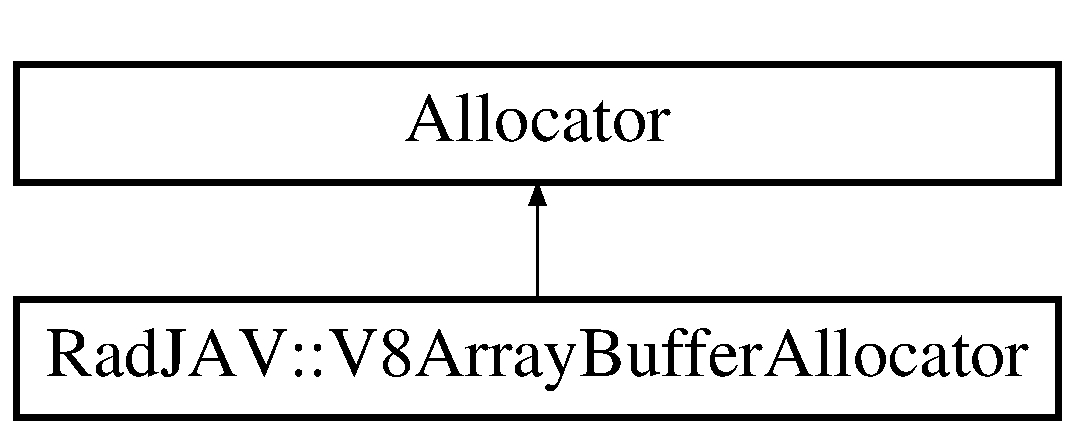
\includegraphics[height=2.000000cm]{class_rad_j_a_v_1_1_v8_array_buffer_allocator}
\end{center}
\end{figure}
\subsection*{Public Member Functions}
\begin{DoxyCompactItemize}
\item 
void $\ast$ \hyperlink{class_rad_j_a_v_1_1_v8_array_buffer_allocator_a3d01e3a6442b8dcb8d4905f91f56bc03}{Allocate} (size\+\_\+t length)
\item 
void $\ast$ \hyperlink{class_rad_j_a_v_1_1_v8_array_buffer_allocator_a11d4ca11d80a94a04c68785ad69622ea}{Allocate\+Uninitialized} (size\+\_\+t length)
\item 
void \hyperlink{class_rad_j_a_v_1_1_v8_array_buffer_allocator_ad1a8dae221c3fb45f6280a4e0841a90e}{Free} (void $\ast$data, size\+\_\+t length)
\end{DoxyCompactItemize}


\subsection{Detailed Description}
The array buffer allocator used for V8. 

\subsection{Member Function Documentation}
\index{Rad\+J\+A\+V\+::\+V8\+Array\+Buffer\+Allocator@{Rad\+J\+A\+V\+::\+V8\+Array\+Buffer\+Allocator}!Allocate@{Allocate}}
\index{Allocate@{Allocate}!Rad\+J\+A\+V\+::\+V8\+Array\+Buffer\+Allocator@{Rad\+J\+A\+V\+::\+V8\+Array\+Buffer\+Allocator}}
\subsubsection[{\texorpdfstring{Allocate(size\+\_\+t length)}{Allocate(size_t length)}}]{\setlength{\rightskip}{0pt plus 5cm}void $\ast$ Rad\+J\+A\+V\+::\+V8\+Array\+Buffer\+Allocator\+::\+Allocate (
\begin{DoxyParamCaption}
\item[{size\+\_\+t}]{length}
\end{DoxyParamCaption}
)}\hypertarget{class_rad_j_a_v_1_1_v8_array_buffer_allocator_a3d01e3a6442b8dcb8d4905f91f56bc03}{}\label{class_rad_j_a_v_1_1_v8_array_buffer_allocator_a3d01e3a6442b8dcb8d4905f91f56bc03}
\index{Rad\+J\+A\+V\+::\+V8\+Array\+Buffer\+Allocator@{Rad\+J\+A\+V\+::\+V8\+Array\+Buffer\+Allocator}!Allocate\+Uninitialized@{Allocate\+Uninitialized}}
\index{Allocate\+Uninitialized@{Allocate\+Uninitialized}!Rad\+J\+A\+V\+::\+V8\+Array\+Buffer\+Allocator@{Rad\+J\+A\+V\+::\+V8\+Array\+Buffer\+Allocator}}
\subsubsection[{\texorpdfstring{Allocate\+Uninitialized(size\+\_\+t length)}{AllocateUninitialized(size_t length)}}]{\setlength{\rightskip}{0pt plus 5cm}void $\ast$ Rad\+J\+A\+V\+::\+V8\+Array\+Buffer\+Allocator\+::\+Allocate\+Uninitialized (
\begin{DoxyParamCaption}
\item[{size\+\_\+t}]{length}
\end{DoxyParamCaption}
)}\hypertarget{class_rad_j_a_v_1_1_v8_array_buffer_allocator_a11d4ca11d80a94a04c68785ad69622ea}{}\label{class_rad_j_a_v_1_1_v8_array_buffer_allocator_a11d4ca11d80a94a04c68785ad69622ea}
\index{Rad\+J\+A\+V\+::\+V8\+Array\+Buffer\+Allocator@{Rad\+J\+A\+V\+::\+V8\+Array\+Buffer\+Allocator}!Free@{Free}}
\index{Free@{Free}!Rad\+J\+A\+V\+::\+V8\+Array\+Buffer\+Allocator@{Rad\+J\+A\+V\+::\+V8\+Array\+Buffer\+Allocator}}
\subsubsection[{\texorpdfstring{Free(void $\ast$data, size\+\_\+t length)}{Free(void *data, size_t length)}}]{\setlength{\rightskip}{0pt plus 5cm}void Rad\+J\+A\+V\+::\+V8\+Array\+Buffer\+Allocator\+::\+Free (
\begin{DoxyParamCaption}
\item[{void $\ast$}]{data, }
\item[{size\+\_\+t}]{length}
\end{DoxyParamCaption}
)}\hypertarget{class_rad_j_a_v_1_1_v8_array_buffer_allocator_ad1a8dae221c3fb45f6280a4e0841a90e}{}\label{class_rad_j_a_v_1_1_v8_array_buffer_allocator_ad1a8dae221c3fb45f6280a4e0841a90e}


The documentation for this class was generated from the following files\+:\begin{DoxyCompactItemize}
\item 
include/\+Rad\+Jav/\hyperlink{_rad_jav_v8_javascript_engine_8h}{Rad\+Jav\+V8\+Javascript\+Engine.\+h}\item 
src/\+Rad\+Jav/\hyperlink{_rad_jav_v8_javascript_engine_8cpp}{Rad\+Jav\+V8\+Javascript\+Engine.\+cpp}\end{DoxyCompactItemize}

\hypertarget{class_rad_j_a_v_1_1_v8_javascript_engine}{}\section{Rad\+J\+AV\+:\+:V8\+Javascript\+Engine Class Reference}
\label{class_rad_j_a_v_1_1_v8_javascript_engine}\index{Rad\+J\+A\+V\+::\+V8\+Javascript\+Engine@{Rad\+J\+A\+V\+::\+V8\+Javascript\+Engine}}


The V8 javascript engine.  




{\ttfamily \#include $<$Rad\+Jav\+V8\+Javascript\+Engine.\+h$>$}

Inheritance diagram for Rad\+J\+AV\+:\+:V8\+Javascript\+Engine\+:\begin{figure}[H]
\begin{center}
\leavevmode
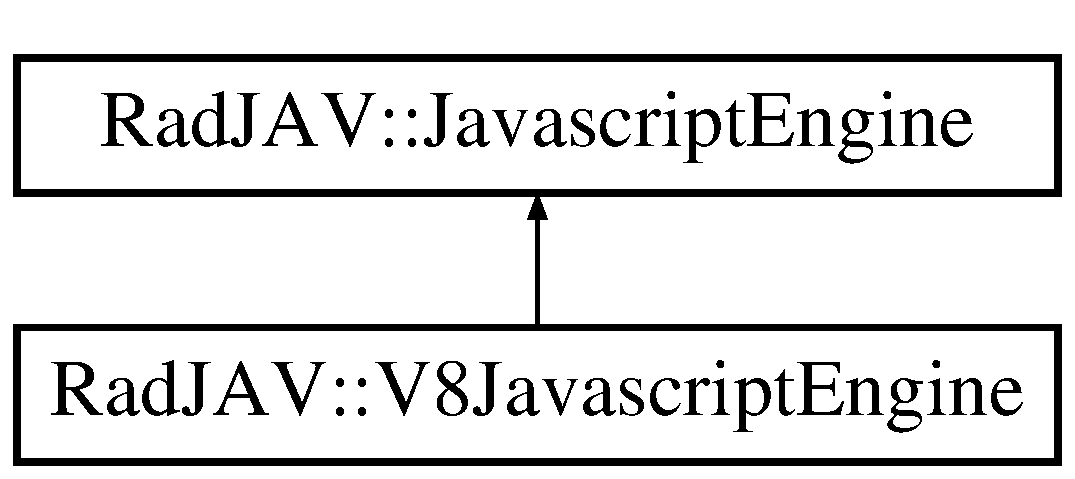
\includegraphics[height=2.000000cm]{class_rad_j_a_v_1_1_v8_javascript_engine}
\end{center}
\end{figure}
\subsection*{Public Member Functions}
\begin{DoxyCompactItemize}
\item 
\mbox{\hyperlink{class_rad_j_a_v_1_1_v8_javascript_engine_ae042dd701a9a521642c2b3daffd7b016}{V8\+Javascript\+Engine}} ()
\item 
\mbox{\hyperlink{class_rad_j_a_v_1_1_v8_javascript_engine_a067369088e8eb2727ed8816d949868a7}{$\sim$\+V8\+Javascript\+Engine}} ()
\item 
void \mbox{\hyperlink{class_rad_j_a_v_1_1_v8_javascript_engine_a85fca2239b08a4c600e5f1269dabf948}{start\+Inspector}} ()
\begin{DoxyCompactList}\small\item\em Start the inspector. \end{DoxyCompactList}\item 
void \mbox{\hyperlink{class_rad_j_a_v_1_1_v8_javascript_engine_af792154ac1ceaa6c65faf2409cea5014}{run\+Application}} (\mbox{\hyperlink{class_rad_j_a_v_1_1_string}{String}} application\+Source, \mbox{\hyperlink{class_rad_j_a_v_1_1_string}{String}} file\+Name)
\begin{DoxyCompactList}\small\item\em Run an application. \end{DoxyCompactList}\item 
void \mbox{\hyperlink{class_rad_j_a_v_1_1_v8_javascript_engine_aa0d9d2f20abcf434f8986f7417ebcc3e}{run\+Application\+From\+File}} (\mbox{\hyperlink{class_rad_j_a_v_1_1_string}{String}} file)
\begin{DoxyCompactList}\small\item\em Run an application from a javascript file. \end{DoxyCompactList}\item 
void \mbox{\hyperlink{class_rad_j_a_v_1_1_v8_javascript_engine_ac45d45c9a25fe8f0f9e90fe21e8ef035}{execute\+Script}} (\mbox{\hyperlink{class_rad_j_a_v_1_1_string}{String}} code, \mbox{\hyperlink{class_rad_j_a_v_1_1_string}{String}} file\+Name)
\begin{DoxyCompactList}\small\item\em Execute Javascript code. \end{DoxyCompactList}\item 
void \mbox{\hyperlink{class_rad_j_a_v_1_1_v8_javascript_engine_a6b6b18af2efefb9c3025310f02ab9596}{execute\+Script}} (\mbox{\hyperlink{class_rad_j_a_v_1_1_string}{String}} code, \mbox{\hyperlink{class_rad_j_a_v_1_1_string}{String}} file\+Name, v8\+::\+Local$<$ v8\+::\+Object $>$ context)
\begin{DoxyCompactList}\small\item\em Execute Javascript code. \end{DoxyCompactList}\item 
void \mbox{\hyperlink{class_rad_j_a_v_1_1_v8_javascript_engine_af5d6bcaa4575a6a1f724029365139c65}{unbounded\+Execute\+Script}} (\mbox{\hyperlink{class_rad_j_a_v_1_1_string}{String}} code, \mbox{\hyperlink{class_rad_j_a_v_1_1_string}{String}} file\+Name, v8\+::\+Local$<$ v8\+::\+Object $>$ context=v8\+::\+Local$<$ v8\+::\+Object $>$())
\begin{DoxyCompactList}\small\item\em Execute unbounded Javascript code. \end{DoxyCompactList}\item 
void \mbox{\hyperlink{class_rad_j_a_v_1_1_v8_javascript_engine_ad3054e8230802a30234d00f1df067701}{execute\+Script\+Next\+Tick}} (\mbox{\hyperlink{class_rad_j_a_v_1_1_string}{String}} code, \mbox{\hyperlink{class_rad_j_a_v_1_1_string}{String}} file\+Name, v8\+::\+Local$<$ v8\+::\+Object $>$ context=v8\+::\+Local$<$ v8\+::\+Object $>$())
\begin{DoxyCompactList}\small\item\em Execute javascript on the next tick. \end{DoxyCompactList}\item 
void \mbox{\hyperlink{class_rad_j_a_v_1_1_v8_javascript_engine_aa282f0464eebfd2a9ae53aea94853870}{call\+Function\+On\+Next\+Tick}} (v8\+::\+Persistent$<$ v8\+::\+Function $>$ $\ast$func, v8\+::\+Persistent$<$ v8\+::\+Array $>$ $\ast$args=N\+U\+LL, R\+J\+B\+O\+OL delete\+On\+Complete=true)
\begin{DoxyCompactList}\small\item\em Call a function on the next tick. Any args passed M\+U\+ST be an array. \end{DoxyCompactList}\item 
void \mbox{\hyperlink{class_rad_j_a_v_1_1_v8_javascript_engine_afd8d4baa780d5ee7a77754eb5ca52e4d}{load\+Native\+Code}} ()
\begin{DoxyCompactList}\small\item\em Connect the native library to the Javascript library. \end{DoxyCompactList}\item 
void \mbox{\hyperlink{class_rad_j_a_v_1_1_v8_javascript_engine_ab9624aca14bbbcb2bb248d81efe8e402}{collect\+Garbage}} ()
\begin{DoxyCompactList}\small\item\em Collect the garbage. This will only work if the engine is started with expose\+GC = true. \end{DoxyCompactList}\item 
void \mbox{\hyperlink{class_rad_j_a_v_1_1_v8_javascript_engine_ae2e4091f33966a1d722690bcd69f2cde}{start3\+D\+Engine}} ()
\begin{DoxyCompactList}\small\item\em Start the 3d engine. \end{DoxyCompactList}\item 
void \mbox{\hyperlink{class_rad_j_a_v_1_1_v8_javascript_engine_ad2c9ab23eb0f84c5776afb6e9e2ed006}{add\+Timeout}} (v8\+::\+Persistent$<$ v8\+::\+Function $>$ $\ast$func, R\+J\+I\+NT time)
\begin{DoxyCompactList}\small\item\em Add a timeout, process it. \end{DoxyCompactList}\item 
void \mbox{\hyperlink{class_rad_j_a_v_1_1_v8_javascript_engine_a13490748bc843ae2d2be22aa889e8e30}{blockchain\+Event}} (\mbox{\hyperlink{class_rad_j_a_v_1_1_string}{String}} event, \mbox{\hyperlink{class_rad_j_a_v_1_1_string}{String}} data\+Type=\char`\"{}null\char`\"{}, void $\ast$data=N\+U\+LL)
\begin{DoxyCompactList}\small\item\em A blockchain event has occurred, process it. \end{DoxyCompactList}\item 
void \mbox{\hyperlink{class_rad_j_a_v_1_1_v8_javascript_engine_adc3d7c751504d623017852ea8bfde1d2}{blockchain\+Event}} (\mbox{\hyperlink{class_rad_j_a_v_1_1_string}{String}} event, R\+J\+I\+NT numargs, v8\+::\+Local$<$ v8\+::\+Value $>$ $\ast$args, R\+J\+B\+O\+OL already\+Entered\+Critial\+Section=false)
\item 
void \mbox{\hyperlink{class_rad_j_a_v_1_1_v8_javascript_engine_ab72b1bfbf3740039b0ae00008a5e4dd3}{add\+Thread}} (\mbox{\hyperlink{class_rad_j_a_v_1_1_thread}{Thread}} $\ast$thread)
\begin{DoxyCompactList}\small\item\em Add a thread to be handled by the engine. \end{DoxyCompactList}\item 
void \mbox{\hyperlink{class_rad_j_a_v_1_1_v8_javascript_engine_a90a52c8c7d655d2e8e5e682d7618c2ab}{remove\+Thread}} (\mbox{\hyperlink{class_rad_j_a_v_1_1_thread}{Thread}} $\ast$thread)
\begin{DoxyCompactList}\small\item\em Remove a thread. \end{DoxyCompactList}\item 
void \mbox{\hyperlink{class_rad_j_a_v_1_1_v8_javascript_engine_a08ad9464e2efe78b0c84d32728b12632}{throw\+Exception}} (\mbox{\hyperlink{class_rad_j_a_v_1_1_string}{String}} message)
\begin{DoxyCompactList}\small\item\em Throw a Javascript exception. \end{DoxyCompactList}\item 
void \mbox{\hyperlink{class_rad_j_a_v_1_1_v8_javascript_engine_a23fcc70cb6805867951748fd1c9706f1}{exit}} (R\+J\+I\+NT exit\+Code)
\begin{DoxyCompactList}\small\item\em Shutdown the application entirely. \end{DoxyCompactList}\item 
v8\+::\+Handle$<$ v8\+::\+Function $>$ \mbox{\hyperlink{class_rad_j_a_v_1_1_v8_javascript_engine_a4470255c90c9b8b56a287a2078feefe3}{v8\+Get\+Function}} (v8\+::\+Local$<$ v8\+::\+Object $>$ context, \mbox{\hyperlink{class_rad_j_a_v_1_1_string}{String}} function\+Name)
\begin{DoxyCompactList}\small\item\em Get a V8 function. \end{DoxyCompactList}\item 
v8\+::\+Handle$<$ v8\+::\+Value $>$ \mbox{\hyperlink{class_rad_j_a_v_1_1_v8_javascript_engine_a3e1e2a736c2fbddc4365cafa94615833}{v8\+Get\+Value}} (v8\+::\+Local$<$ v8\+::\+Object $>$ context, \mbox{\hyperlink{class_rad_j_a_v_1_1_string}{String}} function\+Name)
\begin{DoxyCompactList}\small\item\em Get a V8 value. \end{DoxyCompactList}\item 
void \mbox{\hyperlink{class_rad_j_a_v_1_1_v8_javascript_engine_abe037103f725ff0bd14fdc07ec1d82c8}{v8\+Set\+String}} (v8\+::\+Local$<$ v8\+::\+Object $>$ context, \mbox{\hyperlink{class_rad_j_a_v_1_1_string}{String}} function\+Name, \mbox{\hyperlink{class_rad_j_a_v_1_1_string}{String}} str)
\begin{DoxyCompactList}\small\item\em Set a string. \end{DoxyCompactList}\item 
\mbox{\hyperlink{class_rad_j_a_v_1_1_string}{String}} \mbox{\hyperlink{class_rad_j_a_v_1_1_v8_javascript_engine_a7a92772c801855c5af4dd2afb5dbadca}{v8\+Get\+String}} (v8\+::\+Local$<$ v8\+::\+Object $>$ context, \mbox{\hyperlink{class_rad_j_a_v_1_1_string}{String}} function\+Name)
\begin{DoxyCompactList}\small\item\em Get a string from a V8 variable name. If the value is null or has an empty handle, an empty string will return. \end{DoxyCompactList}\item 
void \mbox{\hyperlink{class_rad_j_a_v_1_1_v8_javascript_engine_a05a3133ff9eba6aebe30e0678a2d8f41}{v8\+Set\+Number}} (v8\+::\+Local$<$ v8\+::\+Object $>$ context, \mbox{\hyperlink{class_rad_j_a_v_1_1_string}{String}} function\+Name, R\+D\+E\+C\+I\+M\+AL number)
\begin{DoxyCompactList}\small\item\em Set a number. \end{DoxyCompactList}\item 
R\+J\+I\+NT \mbox{\hyperlink{class_rad_j_a_v_1_1_v8_javascript_engine_ae9933ac14e6e4a7ad570d28a9d5d75d2}{v8\+Get\+Int}} (v8\+::\+Local$<$ v8\+::\+Object $>$ context, \mbox{\hyperlink{class_rad_j_a_v_1_1_string}{String}} function\+Name)
\begin{DoxyCompactList}\small\item\em Get a V8 int. If the value is null or has an empty handle, 0 will be returned. \end{DoxyCompactList}\item 
R\+D\+E\+C\+I\+M\+AL \mbox{\hyperlink{class_rad_j_a_v_1_1_v8_javascript_engine_a27221a196a2a0d65c687c013c71cf5c0}{v8\+Get\+Decimal}} (v8\+::\+Local$<$ v8\+::\+Object $>$ context, \mbox{\hyperlink{class_rad_j_a_v_1_1_string}{String}} function\+Name)
\begin{DoxyCompactList}\small\item\em Get a V8 decimal. If the value is null or has an empty handle, 0 will be returned. \end{DoxyCompactList}\item 
void \mbox{\hyperlink{class_rad_j_a_v_1_1_v8_javascript_engine_a063f58908a039df554d99bffd8883cb5}{v8\+Set\+Bool}} (v8\+::\+Local$<$ v8\+::\+Object $>$ context, \mbox{\hyperlink{class_rad_j_a_v_1_1_string}{String}} function\+Name, bool value)
\begin{DoxyCompactList}\small\item\em Set a bool from a V8 boolean value. \end{DoxyCompactList}\item 
R\+J\+B\+O\+OL \mbox{\hyperlink{class_rad_j_a_v_1_1_v8_javascript_engine_a688c6447c659170b028377150859996c}{v8\+Get\+Bool}} (v8\+::\+Local$<$ v8\+::\+Object $>$ context, \mbox{\hyperlink{class_rad_j_a_v_1_1_string}{String}} function\+Name)
\begin{DoxyCompactList}\small\item\em Get a V8 bool. If the value is null or has an empty handle, false will be returned. \end{DoxyCompactList}\item 
void \mbox{\hyperlink{class_rad_j_a_v_1_1_v8_javascript_engine_af8bcd13608787e3d2eef9287c2b27b40}{v8\+Set\+Object}} (v8\+::\+Local$<$ v8\+::\+Object $>$ context, \mbox{\hyperlink{class_rad_j_a_v_1_1_string}{String}} function\+Name, v8\+::\+Handle$<$ v8\+::\+Object $>$ obj)
\begin{DoxyCompactList}\small\item\em Set a V8 object. \end{DoxyCompactList}\item 
v8\+::\+Handle$<$ v8\+::\+Object $>$ \mbox{\hyperlink{class_rad_j_a_v_1_1_v8_javascript_engine_a2dd95ba66026d628daaf579cca1b0504}{v8\+Get\+Object}} (v8\+::\+Local$<$ v8\+::\+Object $>$ context, \mbox{\hyperlink{class_rad_j_a_v_1_1_string}{String}} function\+Name)
\begin{DoxyCompactList}\small\item\em Get a V8 object. \end{DoxyCompactList}\item 
v8\+::\+Local$<$ v8\+::\+Value $>$ \mbox{\hyperlink{class_rad_j_a_v_1_1_v8_javascript_engine_ade8a5121713c49ba07afcfd38d8c7960}{v8\+Call\+Function}} (v8\+::\+Local$<$ v8\+::\+Object $>$ context, \mbox{\hyperlink{class_rad_j_a_v_1_1_string}{String}} function\+Name, R\+J\+I\+NT num\+Args, v8\+::\+Local$<$ v8\+::\+Value $>$ $\ast$args)
\begin{DoxyCompactList}\small\item\em Call a V8 function. \end{DoxyCompactList}\item 
v8\+::\+Local$<$ v8\+::\+Object $>$ \mbox{\hyperlink{class_rad_j_a_v_1_1_v8_javascript_engine_a69ece27850f67c44a45292377f953823}{v8\+Call\+As\+Constructor}} (v8\+::\+Local$<$ v8\+::\+Object $>$ function, R\+J\+I\+NT num\+Args, v8\+::\+Local$<$ v8\+::\+Value $>$ $\ast$args)
\begin{DoxyCompactList}\small\item\em Call a V8 function as a constructor. \end{DoxyCompactList}\item 
void $\ast$ \mbox{\hyperlink{class_rad_j_a_v_1_1_v8_javascript_engine_a85e3f8d1a8da39f1197fabb6a1f1825d}{v8\+Get\+External}} (v8\+::\+Local$<$ v8\+::\+Object $>$ context, \mbox{\hyperlink{class_rad_j_a_v_1_1_string}{String}} function\+Name)
\begin{DoxyCompactList}\small\item\em Get a V8 native object. \end{DoxyCompactList}\item 
void \mbox{\hyperlink{class_rad_j_a_v_1_1_v8_javascript_engine_a5ebb5a5ca3ff577e0f32b16eb36827de}{v8\+Set\+External}} (v8\+::\+Local$<$ v8\+::\+Object $>$ context, \mbox{\hyperlink{class_rad_j_a_v_1_1_string}{String}} function\+Name, void $\ast$obj)
\begin{DoxyCompactList}\small\item\em Set a V8 native object. \end{DoxyCompactList}\item 
v8\+::\+Handle$<$ v8\+::\+Value $>$ \mbox{\hyperlink{class_rad_j_a_v_1_1_v8_javascript_engine_abbbd4c175913d3f27ee78d5a9a695571}{v8\+Get\+Argument}} (const v8\+::\+Function\+Callback\+Info$<$ v8\+::\+Value $>$ \&args, R\+J\+U\+I\+NT index)
\begin{DoxyCompactList}\small\item\em Get a V8 argument. \end{DoxyCompactList}\item 
void \mbox{\hyperlink{class_rad_j_a_v_1_1_v8_javascript_engine_a8d4bf88adc107aab88240b3bf1506593}{v8\+Set\+Value}} (v8\+::\+Local$<$ v8\+::\+Object $>$ context, \mbox{\hyperlink{class_rad_j_a_v_1_1_string}{String}} function\+Name, v8\+::\+Handle$<$ v8\+::\+Value $>$ obj)
\begin{DoxyCompactList}\small\item\em Set a V8 Value. \end{DoxyCompactList}\item 
bool \mbox{\hyperlink{class_rad_j_a_v_1_1_v8_javascript_engine_a4a972f2fd1b201f4c1d71926a6db0a56}{v8\+Is\+Null}} (v8\+::\+Local$<$ v8\+::\+Value $>$ val)
\begin{DoxyCompactList}\small\item\em Checks if a V8 value is undefined, null, or if the handle is empty. Returns true if it is. \end{DoxyCompactList}\item 
R\+J\+B\+O\+OL \mbox{\hyperlink{class_rad_j_a_v_1_1_v8_javascript_engine_a37593cc12296ff07e31b6f12d5aa2514}{v8\+Parse\+Bool}} (v8\+::\+Local$<$ v8\+::\+Value $>$ val)
\begin{DoxyCompactList}\small\item\em Get a bool value from a V8 value. \end{DoxyCompactList}\item 
R\+J\+I\+NT \mbox{\hyperlink{class_rad_j_a_v_1_1_v8_javascript_engine_a84c962d7d592cb90fb2b5650c1c4ebac}{v8\+Parse\+Int}} (v8\+::\+Local$<$ v8\+::\+Value $>$ val)
\begin{DoxyCompactList}\small\item\em Get an integer value from a V8 value. \end{DoxyCompactList}\item 
R\+D\+E\+C\+I\+M\+AL \mbox{\hyperlink{class_rad_j_a_v_1_1_v8_javascript_engine_a4be2d9f0eb007b9bff3b8cde3dca41ec}{v8\+Parse\+Decimal}} (v8\+::\+Local$<$ v8\+::\+Value $>$ val)
\begin{DoxyCompactList}\small\item\em Get a decimal value from a V8 value. \end{DoxyCompactList}\item 
v8\+::\+Local$<$ v8\+::\+Object $>$ \mbox{\hyperlink{class_rad_j_a_v_1_1_v8_javascript_engine_ae50f236f667aa73f1cc5b36fc79bfeda}{create\+Promise}} (v8\+::\+Local$<$ v8\+::\+Function $>$ function)
\item 
v8\+::\+Local$<$ v8\+::\+Object $>$ \mbox{\hyperlink{class_rad_j_a_v_1_1_v8_javascript_engine_aeba84f96b6350917eed87a9fc46bff9d}{create\+Promise}} (v8\+::\+Local$<$ v8\+::\+Object $>$ context, v8\+::\+Local$<$ v8\+::\+Function $>$ function, v8\+::\+Local$<$ v8\+::\+Array $>$ args=v8\+::\+Local$<$ v8\+::\+Array $>$())
\end{DoxyCompactItemize}
\subsection*{Static Public Member Functions}
\begin{DoxyCompactItemize}
\item 
static void \mbox{\hyperlink{class_rad_j_a_v_1_1_v8_javascript_engine_aacc9572ce9cc0e4c9977fa588adfe5f6}{load\+Templates}} (const v8\+::\+Function\+Callback\+Info$<$ v8\+::\+Value $>$ \&args)
\begin{DoxyCompactList}\small\item\em Load the native templates into the javascript library. \end{DoxyCompactList}\item 
static void \mbox{\hyperlink{class_rad_j_a_v_1_1_v8_javascript_engine_a724d0548650a735ceac32239f8442a20}{run\+Event\+Loop\+Single\+Step}} (const v8\+::\+Function\+Callback\+Info$<$ v8\+::\+Value $>$ \&args)
\begin{DoxyCompactList}\small\item\em Run the event loop. \end{DoxyCompactList}\item 
static void \mbox{\hyperlink{class_rad_j_a_v_1_1_v8_javascript_engine_a4564a04928c0dd79e002ed74b9dc6b5e}{run\+Script}} (const v8\+::\+Function\+Callback\+Info$<$ v8\+::\+Value $>$ \&args)
\begin{DoxyCompactList}\small\item\em Run a script. \end{DoxyCompactList}\end{DoxyCompactItemize}
\subsection*{Public Attributes}
\begin{DoxyCompactItemize}
\item 
\mbox{\hyperlink{class_rad_j_a_v_1_1_array}{Array}}$<$ v8\+::\+Persistent$<$ v8\+::\+Value, v8\+::\+Copyable\+Persistent\+Traits$<$ v8\+::\+Value $>$ $>$ $\ast$ $>$ \mbox{\hyperlink{class_rad_j_a_v_1_1_v8_javascript_engine_ac2ecff7e8c02bef18a9b23e776b183c9}{persistent\+Data}}
\begin{DoxyCompactList}\small\item\em Destroy an object from v8. \end{DoxyCompactList}\item 
v8\+::\+Isolate $\ast$ \mbox{\hyperlink{class_rad_j_a_v_1_1_v8_javascript_engine_a41236f05ac4ee41c64a9b5d913a19a32}{isolate}}
\begin{DoxyCompactList}\small\item\em The V8 isolate. \end{DoxyCompactList}\item 
v8\+::\+Platform $\ast$ \mbox{\hyperlink{class_rad_j_a_v_1_1_v8_javascript_engine_a6fe5450e6b86a5885af9a3601bcc8ea1}{platform}}
\item 
v8\+::\+Local$<$ v8\+::\+Context $>$ \mbox{\hyperlink{class_rad_j_a_v_1_1_v8_javascript_engine_a0990155ad5fa72dbb88988beb6bf767e}{global\+Context}}
\item 
v8\+::\+Persistent$<$ v8\+::\+Object $>$ $\ast$ \mbox{\hyperlink{class_rad_j_a_v_1_1_v8_javascript_engine_a6a6562df248aedfaf92dceecbee9c777}{rad\+Jav}}
\item 
wx\+Critical\+Section $\ast$ \mbox{\hyperlink{class_rad_j_a_v_1_1_v8_javascript_engine_a1585d63e5888148ed80dfd589f1f5c52}{critical\+Section}}
\end{DoxyCompactItemize}
\subsection*{Protected Attributes}
\begin{DoxyCompactItemize}
\item 
\mbox{\hyperlink{class_rad_j_a_v_1_1_array}{Array}}$<$ \mbox{\hyperlink{class_rad_j_a_v_1_1_string}{String}} $>$ \mbox{\hyperlink{class_rad_j_a_v_1_1_v8_javascript_engine_aee56cac86a4df71bf44c8bf4df05ab0f}{js\+To\+Execute\+Next\+Code}}
\item 
\mbox{\hyperlink{class_rad_j_a_v_1_1_array}{Array}}$<$ \mbox{\hyperlink{class_rad_j_a_v_1_1_string}{String}} $>$ \mbox{\hyperlink{class_rad_j_a_v_1_1_v8_javascript_engine_a7ad75e0d7bc5d1f2710c0b5ce82c6fa8}{js\+To\+Execute\+Next\+Filename}}
\item 
\mbox{\hyperlink{class_rad_j_a_v_1_1_array}{Array}}$<$ v8\+::\+Local$<$ v8\+::\+Object $>$ $>$ \mbox{\hyperlink{class_rad_j_a_v_1_1_v8_javascript_engine_a4f4ed922cbd92c5271639bfb6c86f5e0}{js\+To\+Execute\+Next\+Context}}
\item 
\mbox{\hyperlink{class_rad_j_a_v_1_1_array}{Array}}$<$ v8\+::\+Persistent$<$ v8\+::\+Function $>$ $\ast$ $>$ \mbox{\hyperlink{class_rad_j_a_v_1_1_v8_javascript_engine_a4f0245214c2db2b326d17682797f1f63}{func\+Next}}
\item 
\mbox{\hyperlink{class_rad_j_a_v_1_1_array}{Array}}$<$ v8\+::\+Persistent$<$ v8\+::\+Array $>$ $\ast$ $>$ \mbox{\hyperlink{class_rad_j_a_v_1_1_v8_javascript_engine_a27673918aa575066824d56c9d033bac2}{func\+Next\+Args}}
\item 
\mbox{\hyperlink{class_rad_j_a_v_1_1_array}{Array}}$<$ R\+J\+B\+O\+OL $>$ \mbox{\hyperlink{class_rad_j_a_v_1_1_v8_javascript_engine_a5aff3b1ae19e0782040c87f5205e0574}{func\+Delete}}
\item 
\mbox{\hyperlink{class_rad_j_a_v_1_1_array}{Array}}$<$ v8\+::\+Persistent$<$ v8\+::\+Function $>$ $\ast$ $>$ \mbox{\hyperlink{class_rad_j_a_v_1_1_v8_javascript_engine_a2cee06b34099a70d6efff924d81baf9d}{timeout\+Funcs}}
\item 
\mbox{\hyperlink{class_rad_j_a_v_1_1_array}{Array}}$<$ R\+J\+I\+NT $>$ \mbox{\hyperlink{class_rad_j_a_v_1_1_v8_javascript_engine_aedaa033cba92c65a288c3135a2dbe3f8}{timeouts}}
\item 
R\+J\+B\+O\+OL \mbox{\hyperlink{class_rad_j_a_v_1_1_v8_javascript_engine_a4810bdb10c5af9225f69ec2b7d8bb699}{use\+Inspector}}
\end{DoxyCompactItemize}


\subsection{Detailed Description}
The V8 javascript engine. 

\subsection{Constructor \& Destructor Documentation}
\mbox{\Hypertarget{class_rad_j_a_v_1_1_v8_javascript_engine_ae042dd701a9a521642c2b3daffd7b016}\label{class_rad_j_a_v_1_1_v8_javascript_engine_ae042dd701a9a521642c2b3daffd7b016}} 
\index{Rad\+J\+A\+V\+::\+V8\+Javascript\+Engine@{Rad\+J\+A\+V\+::\+V8\+Javascript\+Engine}!V8\+Javascript\+Engine@{V8\+Javascript\+Engine}}
\index{V8\+Javascript\+Engine@{V8\+Javascript\+Engine}!Rad\+J\+A\+V\+::\+V8\+Javascript\+Engine@{Rad\+J\+A\+V\+::\+V8\+Javascript\+Engine}}
\subsubsection{\texorpdfstring{V8\+Javascript\+Engine()}{V8JavascriptEngine()}}
{\footnotesize\ttfamily Rad\+J\+A\+V\+::\+V8\+Javascript\+Engine\+::\+V8\+Javascript\+Engine (\begin{DoxyParamCaption}{ }\end{DoxyParamCaption})}

\mbox{\Hypertarget{class_rad_j_a_v_1_1_v8_javascript_engine_a067369088e8eb2727ed8816d949868a7}\label{class_rad_j_a_v_1_1_v8_javascript_engine_a067369088e8eb2727ed8816d949868a7}} 
\index{Rad\+J\+A\+V\+::\+V8\+Javascript\+Engine@{Rad\+J\+A\+V\+::\+V8\+Javascript\+Engine}!````~V8\+Javascript\+Engine@{$\sim$\+V8\+Javascript\+Engine}}
\index{````~V8\+Javascript\+Engine@{$\sim$\+V8\+Javascript\+Engine}!Rad\+J\+A\+V\+::\+V8\+Javascript\+Engine@{Rad\+J\+A\+V\+::\+V8\+Javascript\+Engine}}
\subsubsection{\texorpdfstring{$\sim$\+V8\+Javascript\+Engine()}{~V8JavascriptEngine()}}
{\footnotesize\ttfamily Rad\+J\+A\+V\+::\+V8\+Javascript\+Engine\+::$\sim$\+V8\+Javascript\+Engine (\begin{DoxyParamCaption}{ }\end{DoxyParamCaption})}



\subsection{Member Function Documentation}
\mbox{\Hypertarget{class_rad_j_a_v_1_1_v8_javascript_engine_ab72b1bfbf3740039b0ae00008a5e4dd3}\label{class_rad_j_a_v_1_1_v8_javascript_engine_ab72b1bfbf3740039b0ae00008a5e4dd3}} 
\index{Rad\+J\+A\+V\+::\+V8\+Javascript\+Engine@{Rad\+J\+A\+V\+::\+V8\+Javascript\+Engine}!add\+Thread@{add\+Thread}}
\index{add\+Thread@{add\+Thread}!Rad\+J\+A\+V\+::\+V8\+Javascript\+Engine@{Rad\+J\+A\+V\+::\+V8\+Javascript\+Engine}}
\subsubsection{\texorpdfstring{add\+Thread()}{addThread()}}
{\footnotesize\ttfamily void Rad\+J\+A\+V\+::\+V8\+Javascript\+Engine\+::add\+Thread (\begin{DoxyParamCaption}\item[{\mbox{\hyperlink{class_rad_j_a_v_1_1_thread}{Thread}} $\ast$}]{thread }\end{DoxyParamCaption})\hspace{0.3cm}{\ttfamily [virtual]}}



Add a thread to be handled by the engine. 



Implements \mbox{\hyperlink{class_rad_j_a_v_1_1_javascript_engine_abfbd3bff5d4eb0e36d3d18347495bbd7}{Rad\+J\+A\+V\+::\+Javascript\+Engine}}.

\mbox{\Hypertarget{class_rad_j_a_v_1_1_v8_javascript_engine_ad2c9ab23eb0f84c5776afb6e9e2ed006}\label{class_rad_j_a_v_1_1_v8_javascript_engine_ad2c9ab23eb0f84c5776afb6e9e2ed006}} 
\index{Rad\+J\+A\+V\+::\+V8\+Javascript\+Engine@{Rad\+J\+A\+V\+::\+V8\+Javascript\+Engine}!add\+Timeout@{add\+Timeout}}
\index{add\+Timeout@{add\+Timeout}!Rad\+J\+A\+V\+::\+V8\+Javascript\+Engine@{Rad\+J\+A\+V\+::\+V8\+Javascript\+Engine}}
\subsubsection{\texorpdfstring{add\+Timeout()}{addTimeout()}}
{\footnotesize\ttfamily void Rad\+J\+A\+V\+::\+V8\+Javascript\+Engine\+::add\+Timeout (\begin{DoxyParamCaption}\item[{v8\+::\+Persistent$<$ v8\+::\+Function $>$ $\ast$}]{func,  }\item[{R\+J\+I\+NT}]{time }\end{DoxyParamCaption})}



Add a timeout, process it. 

\mbox{\Hypertarget{class_rad_j_a_v_1_1_v8_javascript_engine_a13490748bc843ae2d2be22aa889e8e30}\label{class_rad_j_a_v_1_1_v8_javascript_engine_a13490748bc843ae2d2be22aa889e8e30}} 
\index{Rad\+J\+A\+V\+::\+V8\+Javascript\+Engine@{Rad\+J\+A\+V\+::\+V8\+Javascript\+Engine}!blockchain\+Event@{blockchain\+Event}}
\index{blockchain\+Event@{blockchain\+Event}!Rad\+J\+A\+V\+::\+V8\+Javascript\+Engine@{Rad\+J\+A\+V\+::\+V8\+Javascript\+Engine}}
\subsubsection{\texorpdfstring{blockchain\+Event()}{blockchainEvent()}\hspace{0.1cm}{\footnotesize\ttfamily [1/2]}}
{\footnotesize\ttfamily void Rad\+J\+A\+V\+::\+V8\+Javascript\+Engine\+::blockchain\+Event (\begin{DoxyParamCaption}\item[{\mbox{\hyperlink{class_rad_j_a_v_1_1_string}{String}}}]{event,  }\item[{\mbox{\hyperlink{class_rad_j_a_v_1_1_string}{String}}}]{data\+Type = {\ttfamily \char`\"{}null\char`\"{}},  }\item[{void $\ast$}]{data = {\ttfamily NULL} }\end{DoxyParamCaption})\hspace{0.3cm}{\ttfamily [virtual]}}



A blockchain event has occurred, process it. 

\begin{DoxyRefDesc}{Bug}
\item[\mbox{\hyperlink{bug__bug000002}{Bug}}]Stupid hack for now. This will skip any function that needs to execute if a lock can\textquotesingle{}t be placed. \end{DoxyRefDesc}


Implements \mbox{\hyperlink{class_rad_j_a_v_1_1_javascript_engine_a91ebe8029a9658f66d9c39356eea2d80}{Rad\+J\+A\+V\+::\+Javascript\+Engine}}.

\mbox{\Hypertarget{class_rad_j_a_v_1_1_v8_javascript_engine_adc3d7c751504d623017852ea8bfde1d2}\label{class_rad_j_a_v_1_1_v8_javascript_engine_adc3d7c751504d623017852ea8bfde1d2}} 
\index{Rad\+J\+A\+V\+::\+V8\+Javascript\+Engine@{Rad\+J\+A\+V\+::\+V8\+Javascript\+Engine}!blockchain\+Event@{blockchain\+Event}}
\index{blockchain\+Event@{blockchain\+Event}!Rad\+J\+A\+V\+::\+V8\+Javascript\+Engine@{Rad\+J\+A\+V\+::\+V8\+Javascript\+Engine}}
\subsubsection{\texorpdfstring{blockchain\+Event()}{blockchainEvent()}\hspace{0.1cm}{\footnotesize\ttfamily [2/2]}}
{\footnotesize\ttfamily void Rad\+J\+A\+V\+::\+V8\+Javascript\+Engine\+::blockchain\+Event (\begin{DoxyParamCaption}\item[{\mbox{\hyperlink{class_rad_j_a_v_1_1_string}{String}}}]{event,  }\item[{R\+J\+I\+NT}]{numargs,  }\item[{v8\+::\+Local$<$ v8\+::\+Value $>$ $\ast$}]{args,  }\item[{R\+J\+B\+O\+OL}]{already\+Entered\+Critial\+Section = {\ttfamily false} }\end{DoxyParamCaption})}

\begin{DoxyRefDesc}{Bug}
\item[\mbox{\hyperlink{bug__bug000003}{Bug}}]Stupid hack for now. This will skip any function that needs to execute if a lock can\textquotesingle{}t be placed. \end{DoxyRefDesc}
\mbox{\Hypertarget{class_rad_j_a_v_1_1_v8_javascript_engine_aa282f0464eebfd2a9ae53aea94853870}\label{class_rad_j_a_v_1_1_v8_javascript_engine_aa282f0464eebfd2a9ae53aea94853870}} 
\index{Rad\+J\+A\+V\+::\+V8\+Javascript\+Engine@{Rad\+J\+A\+V\+::\+V8\+Javascript\+Engine}!call\+Function\+On\+Next\+Tick@{call\+Function\+On\+Next\+Tick}}
\index{call\+Function\+On\+Next\+Tick@{call\+Function\+On\+Next\+Tick}!Rad\+J\+A\+V\+::\+V8\+Javascript\+Engine@{Rad\+J\+A\+V\+::\+V8\+Javascript\+Engine}}
\subsubsection{\texorpdfstring{call\+Function\+On\+Next\+Tick()}{callFunctionOnNextTick()}}
{\footnotesize\ttfamily void Rad\+J\+A\+V\+::\+V8\+Javascript\+Engine\+::call\+Function\+On\+Next\+Tick (\begin{DoxyParamCaption}\item[{v8\+::\+Persistent$<$ v8\+::\+Function $>$ $\ast$}]{func,  }\item[{v8\+::\+Persistent$<$ v8\+::\+Array $>$ $\ast$}]{args = {\ttfamily NULL},  }\item[{R\+J\+B\+O\+OL}]{delete\+On\+Complete = {\ttfamily true} }\end{DoxyParamCaption})}



Call a function on the next tick. Any args passed M\+U\+ST be an array. 

\mbox{\Hypertarget{class_rad_j_a_v_1_1_v8_javascript_engine_ab9624aca14bbbcb2bb248d81efe8e402}\label{class_rad_j_a_v_1_1_v8_javascript_engine_ab9624aca14bbbcb2bb248d81efe8e402}} 
\index{Rad\+J\+A\+V\+::\+V8\+Javascript\+Engine@{Rad\+J\+A\+V\+::\+V8\+Javascript\+Engine}!collect\+Garbage@{collect\+Garbage}}
\index{collect\+Garbage@{collect\+Garbage}!Rad\+J\+A\+V\+::\+V8\+Javascript\+Engine@{Rad\+J\+A\+V\+::\+V8\+Javascript\+Engine}}
\subsubsection{\texorpdfstring{collect\+Garbage()}{collectGarbage()}}
{\footnotesize\ttfamily void Rad\+J\+A\+V\+::\+V8\+Javascript\+Engine\+::collect\+Garbage (\begin{DoxyParamCaption}{ }\end{DoxyParamCaption})\hspace{0.3cm}{\ttfamily [virtual]}}



Collect the garbage. This will only work if the engine is started with expose\+GC = true. 



Implements \mbox{\hyperlink{class_rad_j_a_v_1_1_javascript_engine_a07709e2f1afb9f49444c6605a7a6122f}{Rad\+J\+A\+V\+::\+Javascript\+Engine}}.

\mbox{\Hypertarget{class_rad_j_a_v_1_1_v8_javascript_engine_ae50f236f667aa73f1cc5b36fc79bfeda}\label{class_rad_j_a_v_1_1_v8_javascript_engine_ae50f236f667aa73f1cc5b36fc79bfeda}} 
\index{Rad\+J\+A\+V\+::\+V8\+Javascript\+Engine@{Rad\+J\+A\+V\+::\+V8\+Javascript\+Engine}!create\+Promise@{create\+Promise}}
\index{create\+Promise@{create\+Promise}!Rad\+J\+A\+V\+::\+V8\+Javascript\+Engine@{Rad\+J\+A\+V\+::\+V8\+Javascript\+Engine}}
\subsubsection{\texorpdfstring{create\+Promise()}{createPromise()}\hspace{0.1cm}{\footnotesize\ttfamily [1/2]}}
{\footnotesize\ttfamily v8\+::\+Local$<$ v8\+::\+Object $>$ Rad\+J\+A\+V\+::\+V8\+Javascript\+Engine\+::create\+Promise (\begin{DoxyParamCaption}\item[{v8\+::\+Local$<$ v8\+::\+Function $>$}]{function }\end{DoxyParamCaption})}

\mbox{\Hypertarget{class_rad_j_a_v_1_1_v8_javascript_engine_aeba84f96b6350917eed87a9fc46bff9d}\label{class_rad_j_a_v_1_1_v8_javascript_engine_aeba84f96b6350917eed87a9fc46bff9d}} 
\index{Rad\+J\+A\+V\+::\+V8\+Javascript\+Engine@{Rad\+J\+A\+V\+::\+V8\+Javascript\+Engine}!create\+Promise@{create\+Promise}}
\index{create\+Promise@{create\+Promise}!Rad\+J\+A\+V\+::\+V8\+Javascript\+Engine@{Rad\+J\+A\+V\+::\+V8\+Javascript\+Engine}}
\subsubsection{\texorpdfstring{create\+Promise()}{createPromise()}\hspace{0.1cm}{\footnotesize\ttfamily [2/2]}}
{\footnotesize\ttfamily v8\+::\+Local$<$ v8\+::\+Object $>$ Rad\+J\+A\+V\+::\+V8\+Javascript\+Engine\+::create\+Promise (\begin{DoxyParamCaption}\item[{v8\+::\+Local$<$ v8\+::\+Object $>$}]{context,  }\item[{v8\+::\+Local$<$ v8\+::\+Function $>$}]{function,  }\item[{v8\+::\+Local$<$ v8\+::\+Array $>$}]{args = {\ttfamily v8\+:\+:Local$<$v8\+:\+:Array$>$~()} }\end{DoxyParamCaption})}

\mbox{\Hypertarget{class_rad_j_a_v_1_1_v8_javascript_engine_ac45d45c9a25fe8f0f9e90fe21e8ef035}\label{class_rad_j_a_v_1_1_v8_javascript_engine_ac45d45c9a25fe8f0f9e90fe21e8ef035}} 
\index{Rad\+J\+A\+V\+::\+V8\+Javascript\+Engine@{Rad\+J\+A\+V\+::\+V8\+Javascript\+Engine}!execute\+Script@{execute\+Script}}
\index{execute\+Script@{execute\+Script}!Rad\+J\+A\+V\+::\+V8\+Javascript\+Engine@{Rad\+J\+A\+V\+::\+V8\+Javascript\+Engine}}
\subsubsection{\texorpdfstring{execute\+Script()}{executeScript()}\hspace{0.1cm}{\footnotesize\ttfamily [1/2]}}
{\footnotesize\ttfamily void Rad\+J\+A\+V\+::\+V8\+Javascript\+Engine\+::execute\+Script (\begin{DoxyParamCaption}\item[{\mbox{\hyperlink{class_rad_j_a_v_1_1_string}{String}}}]{code,  }\item[{\mbox{\hyperlink{class_rad_j_a_v_1_1_string}{String}}}]{file\+Name }\end{DoxyParamCaption})\hspace{0.3cm}{\ttfamily [virtual]}}



Execute Javascript code. 



Implements \mbox{\hyperlink{class_rad_j_a_v_1_1_javascript_engine_a4cdc81e5c398f7f1a2ce3ff45f135792}{Rad\+J\+A\+V\+::\+Javascript\+Engine}}.

\mbox{\Hypertarget{class_rad_j_a_v_1_1_v8_javascript_engine_a6b6b18af2efefb9c3025310f02ab9596}\label{class_rad_j_a_v_1_1_v8_javascript_engine_a6b6b18af2efefb9c3025310f02ab9596}} 
\index{Rad\+J\+A\+V\+::\+V8\+Javascript\+Engine@{Rad\+J\+A\+V\+::\+V8\+Javascript\+Engine}!execute\+Script@{execute\+Script}}
\index{execute\+Script@{execute\+Script}!Rad\+J\+A\+V\+::\+V8\+Javascript\+Engine@{Rad\+J\+A\+V\+::\+V8\+Javascript\+Engine}}
\subsubsection{\texorpdfstring{execute\+Script()}{executeScript()}\hspace{0.1cm}{\footnotesize\ttfamily [2/2]}}
{\footnotesize\ttfamily void Rad\+J\+A\+V\+::\+V8\+Javascript\+Engine\+::execute\+Script (\begin{DoxyParamCaption}\item[{\mbox{\hyperlink{class_rad_j_a_v_1_1_string}{String}}}]{code,  }\item[{\mbox{\hyperlink{class_rad_j_a_v_1_1_string}{String}}}]{file\+Name,  }\item[{v8\+::\+Local$<$ v8\+::\+Object $>$}]{context }\end{DoxyParamCaption})}



Execute Javascript code. 

\mbox{\Hypertarget{class_rad_j_a_v_1_1_v8_javascript_engine_ad3054e8230802a30234d00f1df067701}\label{class_rad_j_a_v_1_1_v8_javascript_engine_ad3054e8230802a30234d00f1df067701}} 
\index{Rad\+J\+A\+V\+::\+V8\+Javascript\+Engine@{Rad\+J\+A\+V\+::\+V8\+Javascript\+Engine}!execute\+Script\+Next\+Tick@{execute\+Script\+Next\+Tick}}
\index{execute\+Script\+Next\+Tick@{execute\+Script\+Next\+Tick}!Rad\+J\+A\+V\+::\+V8\+Javascript\+Engine@{Rad\+J\+A\+V\+::\+V8\+Javascript\+Engine}}
\subsubsection{\texorpdfstring{execute\+Script\+Next\+Tick()}{executeScriptNextTick()}}
{\footnotesize\ttfamily void Rad\+J\+A\+V\+::\+V8\+Javascript\+Engine\+::execute\+Script\+Next\+Tick (\begin{DoxyParamCaption}\item[{\mbox{\hyperlink{class_rad_j_a_v_1_1_string}{String}}}]{code,  }\item[{\mbox{\hyperlink{class_rad_j_a_v_1_1_string}{String}}}]{file\+Name,  }\item[{v8\+::\+Local$<$ v8\+::\+Object $>$}]{context = {\ttfamily v8\+:\+:Local$<$v8\+:\+:Object$>$()} }\end{DoxyParamCaption})}



Execute javascript on the next tick. 

\mbox{\Hypertarget{class_rad_j_a_v_1_1_v8_javascript_engine_a23fcc70cb6805867951748fd1c9706f1}\label{class_rad_j_a_v_1_1_v8_javascript_engine_a23fcc70cb6805867951748fd1c9706f1}} 
\index{Rad\+J\+A\+V\+::\+V8\+Javascript\+Engine@{Rad\+J\+A\+V\+::\+V8\+Javascript\+Engine}!exit@{exit}}
\index{exit@{exit}!Rad\+J\+A\+V\+::\+V8\+Javascript\+Engine@{Rad\+J\+A\+V\+::\+V8\+Javascript\+Engine}}
\subsubsection{\texorpdfstring{exit()}{exit()}}
{\footnotesize\ttfamily void Rad\+J\+A\+V\+::\+V8\+Javascript\+Engine\+::exit (\begin{DoxyParamCaption}\item[{R\+J\+I\+NT}]{exit\+Code }\end{DoxyParamCaption})\hspace{0.3cm}{\ttfamily [virtual]}}



Shutdown the application entirely. 



Implements \mbox{\hyperlink{class_rad_j_a_v_1_1_javascript_engine_a4a720b2e36ab737ab0b697e9b7317fb0}{Rad\+J\+A\+V\+::\+Javascript\+Engine}}.

\mbox{\Hypertarget{class_rad_j_a_v_1_1_v8_javascript_engine_afd8d4baa780d5ee7a77754eb5ca52e4d}\label{class_rad_j_a_v_1_1_v8_javascript_engine_afd8d4baa780d5ee7a77754eb5ca52e4d}} 
\index{Rad\+J\+A\+V\+::\+V8\+Javascript\+Engine@{Rad\+J\+A\+V\+::\+V8\+Javascript\+Engine}!load\+Native\+Code@{load\+Native\+Code}}
\index{load\+Native\+Code@{load\+Native\+Code}!Rad\+J\+A\+V\+::\+V8\+Javascript\+Engine@{Rad\+J\+A\+V\+::\+V8\+Javascript\+Engine}}
\subsubsection{\texorpdfstring{load\+Native\+Code()}{loadNativeCode()}}
{\footnotesize\ttfamily void Rad\+J\+A\+V\+::\+V8\+Javascript\+Engine\+::load\+Native\+Code (\begin{DoxyParamCaption}{ }\end{DoxyParamCaption})\hspace{0.3cm}{\ttfamily [virtual]}}



Connect the native library to the Javascript library. 

Text\+File 

Implements \mbox{\hyperlink{class_rad_j_a_v_1_1_javascript_engine_a91b208b07958c50ce906cd9f25eed669}{Rad\+J\+A\+V\+::\+Javascript\+Engine}}.

\mbox{\Hypertarget{class_rad_j_a_v_1_1_v8_javascript_engine_aacc9572ce9cc0e4c9977fa588adfe5f6}\label{class_rad_j_a_v_1_1_v8_javascript_engine_aacc9572ce9cc0e4c9977fa588adfe5f6}} 
\index{Rad\+J\+A\+V\+::\+V8\+Javascript\+Engine@{Rad\+J\+A\+V\+::\+V8\+Javascript\+Engine}!load\+Templates@{load\+Templates}}
\index{load\+Templates@{load\+Templates}!Rad\+J\+A\+V\+::\+V8\+Javascript\+Engine@{Rad\+J\+A\+V\+::\+V8\+Javascript\+Engine}}
\subsubsection{\texorpdfstring{load\+Templates()}{loadTemplates()}}
{\footnotesize\ttfamily void Rad\+J\+A\+V\+::\+V8\+Javascript\+Engine\+::load\+Templates (\begin{DoxyParamCaption}\item[{const v8\+::\+Function\+Callback\+Info$<$ v8\+::\+Value $>$ \&}]{args }\end{DoxyParamCaption})\hspace{0.3cm}{\ttfamily [static]}}



Load the native templates into the javascript library. 

\mbox{\Hypertarget{class_rad_j_a_v_1_1_v8_javascript_engine_a90a52c8c7d655d2e8e5e682d7618c2ab}\label{class_rad_j_a_v_1_1_v8_javascript_engine_a90a52c8c7d655d2e8e5e682d7618c2ab}} 
\index{Rad\+J\+A\+V\+::\+V8\+Javascript\+Engine@{Rad\+J\+A\+V\+::\+V8\+Javascript\+Engine}!remove\+Thread@{remove\+Thread}}
\index{remove\+Thread@{remove\+Thread}!Rad\+J\+A\+V\+::\+V8\+Javascript\+Engine@{Rad\+J\+A\+V\+::\+V8\+Javascript\+Engine}}
\subsubsection{\texorpdfstring{remove\+Thread()}{removeThread()}}
{\footnotesize\ttfamily void Rad\+J\+A\+V\+::\+V8\+Javascript\+Engine\+::remove\+Thread (\begin{DoxyParamCaption}\item[{\mbox{\hyperlink{class_rad_j_a_v_1_1_thread}{Thread}} $\ast$}]{thread }\end{DoxyParamCaption})\hspace{0.3cm}{\ttfamily [virtual]}}



Remove a thread. 



Implements \mbox{\hyperlink{class_rad_j_a_v_1_1_javascript_engine_afe08c6324e3958a5d3ec82fa9e0f1fd1}{Rad\+J\+A\+V\+::\+Javascript\+Engine}}.

\mbox{\Hypertarget{class_rad_j_a_v_1_1_v8_javascript_engine_af792154ac1ceaa6c65faf2409cea5014}\label{class_rad_j_a_v_1_1_v8_javascript_engine_af792154ac1ceaa6c65faf2409cea5014}} 
\index{Rad\+J\+A\+V\+::\+V8\+Javascript\+Engine@{Rad\+J\+A\+V\+::\+V8\+Javascript\+Engine}!run\+Application@{run\+Application}}
\index{run\+Application@{run\+Application}!Rad\+J\+A\+V\+::\+V8\+Javascript\+Engine@{Rad\+J\+A\+V\+::\+V8\+Javascript\+Engine}}
\subsubsection{\texorpdfstring{run\+Application()}{runApplication()}}
{\footnotesize\ttfamily void Rad\+J\+A\+V\+::\+V8\+Javascript\+Engine\+::run\+Application (\begin{DoxyParamCaption}\item[{\mbox{\hyperlink{class_rad_j_a_v_1_1_string}{String}}}]{application\+Source,  }\item[{\mbox{\hyperlink{class_rad_j_a_v_1_1_string}{String}}}]{file\+Name }\end{DoxyParamCaption})\hspace{0.3cm}{\ttfamily [virtual]}}



Run an application. 

\begin{DoxyRefDesc}{Bug}
\item[\mbox{\hyperlink{bug__bug000001}{Bug}}]tbegin-\/$>$second should be deleted, or does wx\+Widgets delete it automatically? \end{DoxyRefDesc}


Implements \mbox{\hyperlink{class_rad_j_a_v_1_1_javascript_engine_a11cc903f042db2b770183667ee36c6bf}{Rad\+J\+A\+V\+::\+Javascript\+Engine}}.

\mbox{\Hypertarget{class_rad_j_a_v_1_1_v8_javascript_engine_aa0d9d2f20abcf434f8986f7417ebcc3e}\label{class_rad_j_a_v_1_1_v8_javascript_engine_aa0d9d2f20abcf434f8986f7417ebcc3e}} 
\index{Rad\+J\+A\+V\+::\+V8\+Javascript\+Engine@{Rad\+J\+A\+V\+::\+V8\+Javascript\+Engine}!run\+Application\+From\+File@{run\+Application\+From\+File}}
\index{run\+Application\+From\+File@{run\+Application\+From\+File}!Rad\+J\+A\+V\+::\+V8\+Javascript\+Engine@{Rad\+J\+A\+V\+::\+V8\+Javascript\+Engine}}
\subsubsection{\texorpdfstring{run\+Application\+From\+File()}{runApplicationFromFile()}}
{\footnotesize\ttfamily void Rad\+J\+A\+V\+::\+V8\+Javascript\+Engine\+::run\+Application\+From\+File (\begin{DoxyParamCaption}\item[{\mbox{\hyperlink{class_rad_j_a_v_1_1_string}{String}}}]{file }\end{DoxyParamCaption})\hspace{0.3cm}{\ttfamily [virtual]}}



Run an application from a javascript file. 



Implements \mbox{\hyperlink{class_rad_j_a_v_1_1_javascript_engine_a0a435f458e118a813c95ccb359d546e9}{Rad\+J\+A\+V\+::\+Javascript\+Engine}}.

\mbox{\Hypertarget{class_rad_j_a_v_1_1_v8_javascript_engine_a724d0548650a735ceac32239f8442a20}\label{class_rad_j_a_v_1_1_v8_javascript_engine_a724d0548650a735ceac32239f8442a20}} 
\index{Rad\+J\+A\+V\+::\+V8\+Javascript\+Engine@{Rad\+J\+A\+V\+::\+V8\+Javascript\+Engine}!run\+Event\+Loop\+Single\+Step@{run\+Event\+Loop\+Single\+Step}}
\index{run\+Event\+Loop\+Single\+Step@{run\+Event\+Loop\+Single\+Step}!Rad\+J\+A\+V\+::\+V8\+Javascript\+Engine@{Rad\+J\+A\+V\+::\+V8\+Javascript\+Engine}}
\subsubsection{\texorpdfstring{run\+Event\+Loop\+Single\+Step()}{runEventLoopSingleStep()}}
{\footnotesize\ttfamily void Rad\+J\+A\+V\+::\+V8\+Javascript\+Engine\+::run\+Event\+Loop\+Single\+Step (\begin{DoxyParamCaption}\item[{const v8\+::\+Function\+Callback\+Info$<$ v8\+::\+Value $>$ \&}]{args }\end{DoxyParamCaption})\hspace{0.3cm}{\ttfamily [static]}}



Run the event loop. 

\mbox{\Hypertarget{class_rad_j_a_v_1_1_v8_javascript_engine_a4564a04928c0dd79e002ed74b9dc6b5e}\label{class_rad_j_a_v_1_1_v8_javascript_engine_a4564a04928c0dd79e002ed74b9dc6b5e}} 
\index{Rad\+J\+A\+V\+::\+V8\+Javascript\+Engine@{Rad\+J\+A\+V\+::\+V8\+Javascript\+Engine}!run\+Script@{run\+Script}}
\index{run\+Script@{run\+Script}!Rad\+J\+A\+V\+::\+V8\+Javascript\+Engine@{Rad\+J\+A\+V\+::\+V8\+Javascript\+Engine}}
\subsubsection{\texorpdfstring{run\+Script()}{runScript()}}
{\footnotesize\ttfamily void Rad\+J\+A\+V\+::\+V8\+Javascript\+Engine\+::run\+Script (\begin{DoxyParamCaption}\item[{const v8\+::\+Function\+Callback\+Info$<$ v8\+::\+Value $>$ \&}]{args }\end{DoxyParamCaption})\hspace{0.3cm}{\ttfamily [static]}}



Run a script. 

\mbox{\Hypertarget{class_rad_j_a_v_1_1_v8_javascript_engine_ae2e4091f33966a1d722690bcd69f2cde}\label{class_rad_j_a_v_1_1_v8_javascript_engine_ae2e4091f33966a1d722690bcd69f2cde}} 
\index{Rad\+J\+A\+V\+::\+V8\+Javascript\+Engine@{Rad\+J\+A\+V\+::\+V8\+Javascript\+Engine}!start3\+D\+Engine@{start3\+D\+Engine}}
\index{start3\+D\+Engine@{start3\+D\+Engine}!Rad\+J\+A\+V\+::\+V8\+Javascript\+Engine@{Rad\+J\+A\+V\+::\+V8\+Javascript\+Engine}}
\subsubsection{\texorpdfstring{start3\+D\+Engine()}{start3DEngine()}}
{\footnotesize\ttfamily void Rad\+J\+A\+V\+::\+V8\+Javascript\+Engine\+::start3\+D\+Engine (\begin{DoxyParamCaption}{ }\end{DoxyParamCaption})\hspace{0.3cm}{\ttfamily [virtual]}}



Start the 3d engine. 



Implements \mbox{\hyperlink{class_rad_j_a_v_1_1_javascript_engine_a76c00d87d65f69781e2dc4aa3143acac}{Rad\+J\+A\+V\+::\+Javascript\+Engine}}.

\mbox{\Hypertarget{class_rad_j_a_v_1_1_v8_javascript_engine_a85fca2239b08a4c600e5f1269dabf948}\label{class_rad_j_a_v_1_1_v8_javascript_engine_a85fca2239b08a4c600e5f1269dabf948}} 
\index{Rad\+J\+A\+V\+::\+V8\+Javascript\+Engine@{Rad\+J\+A\+V\+::\+V8\+Javascript\+Engine}!start\+Inspector@{start\+Inspector}}
\index{start\+Inspector@{start\+Inspector}!Rad\+J\+A\+V\+::\+V8\+Javascript\+Engine@{Rad\+J\+A\+V\+::\+V8\+Javascript\+Engine}}
\subsubsection{\texorpdfstring{start\+Inspector()}{startInspector()}}
{\footnotesize\ttfamily void Rad\+J\+A\+V\+::\+V8\+Javascript\+Engine\+::start\+Inspector (\begin{DoxyParamCaption}{ }\end{DoxyParamCaption})}



Start the inspector. 

\mbox{\Hypertarget{class_rad_j_a_v_1_1_v8_javascript_engine_a08ad9464e2efe78b0c84d32728b12632}\label{class_rad_j_a_v_1_1_v8_javascript_engine_a08ad9464e2efe78b0c84d32728b12632}} 
\index{Rad\+J\+A\+V\+::\+V8\+Javascript\+Engine@{Rad\+J\+A\+V\+::\+V8\+Javascript\+Engine}!throw\+Exception@{throw\+Exception}}
\index{throw\+Exception@{throw\+Exception}!Rad\+J\+A\+V\+::\+V8\+Javascript\+Engine@{Rad\+J\+A\+V\+::\+V8\+Javascript\+Engine}}
\subsubsection{\texorpdfstring{throw\+Exception()}{throwException()}}
{\footnotesize\ttfamily void Rad\+J\+A\+V\+::\+V8\+Javascript\+Engine\+::throw\+Exception (\begin{DoxyParamCaption}\item[{\mbox{\hyperlink{class_rad_j_a_v_1_1_string}{String}}}]{message }\end{DoxyParamCaption})\hspace{0.3cm}{\ttfamily [virtual]}}



Throw a Javascript exception. 



Implements \mbox{\hyperlink{class_rad_j_a_v_1_1_javascript_engine_ab9f13c1928d6967122d0f9a6a026dc73}{Rad\+J\+A\+V\+::\+Javascript\+Engine}}.

\mbox{\Hypertarget{class_rad_j_a_v_1_1_v8_javascript_engine_af5d6bcaa4575a6a1f724029365139c65}\label{class_rad_j_a_v_1_1_v8_javascript_engine_af5d6bcaa4575a6a1f724029365139c65}} 
\index{Rad\+J\+A\+V\+::\+V8\+Javascript\+Engine@{Rad\+J\+A\+V\+::\+V8\+Javascript\+Engine}!unbounded\+Execute\+Script@{unbounded\+Execute\+Script}}
\index{unbounded\+Execute\+Script@{unbounded\+Execute\+Script}!Rad\+J\+A\+V\+::\+V8\+Javascript\+Engine@{Rad\+J\+A\+V\+::\+V8\+Javascript\+Engine}}
\subsubsection{\texorpdfstring{unbounded\+Execute\+Script()}{unboundedExecuteScript()}}
{\footnotesize\ttfamily void Rad\+J\+A\+V\+::\+V8\+Javascript\+Engine\+::unbounded\+Execute\+Script (\begin{DoxyParamCaption}\item[{\mbox{\hyperlink{class_rad_j_a_v_1_1_string}{String}}}]{code,  }\item[{\mbox{\hyperlink{class_rad_j_a_v_1_1_string}{String}}}]{file\+Name,  }\item[{v8\+::\+Local$<$ v8\+::\+Object $>$}]{context = {\ttfamily v8\+:\+:Local$<$v8\+:\+:Object$>$()} }\end{DoxyParamCaption})}



Execute unbounded Javascript code. 

\mbox{\Hypertarget{class_rad_j_a_v_1_1_v8_javascript_engine_a69ece27850f67c44a45292377f953823}\label{class_rad_j_a_v_1_1_v8_javascript_engine_a69ece27850f67c44a45292377f953823}} 
\index{Rad\+J\+A\+V\+::\+V8\+Javascript\+Engine@{Rad\+J\+A\+V\+::\+V8\+Javascript\+Engine}!v8\+Call\+As\+Constructor@{v8\+Call\+As\+Constructor}}
\index{v8\+Call\+As\+Constructor@{v8\+Call\+As\+Constructor}!Rad\+J\+A\+V\+::\+V8\+Javascript\+Engine@{Rad\+J\+A\+V\+::\+V8\+Javascript\+Engine}}
\subsubsection{\texorpdfstring{v8\+Call\+As\+Constructor()}{v8CallAsConstructor()}}
{\footnotesize\ttfamily v8\+::\+Local$<$ v8\+::\+Object $>$ Rad\+J\+A\+V\+::\+V8\+Javascript\+Engine\+::v8\+Call\+As\+Constructor (\begin{DoxyParamCaption}\item[{v8\+::\+Local$<$ v8\+::\+Object $>$}]{function,  }\item[{R\+J\+I\+NT}]{num\+Args,  }\item[{v8\+::\+Local$<$ v8\+::\+Value $>$ $\ast$}]{args }\end{DoxyParamCaption})}



Call a V8 function as a constructor. 

\mbox{\Hypertarget{class_rad_j_a_v_1_1_v8_javascript_engine_ade8a5121713c49ba07afcfd38d8c7960}\label{class_rad_j_a_v_1_1_v8_javascript_engine_ade8a5121713c49ba07afcfd38d8c7960}} 
\index{Rad\+J\+A\+V\+::\+V8\+Javascript\+Engine@{Rad\+J\+A\+V\+::\+V8\+Javascript\+Engine}!v8\+Call\+Function@{v8\+Call\+Function}}
\index{v8\+Call\+Function@{v8\+Call\+Function}!Rad\+J\+A\+V\+::\+V8\+Javascript\+Engine@{Rad\+J\+A\+V\+::\+V8\+Javascript\+Engine}}
\subsubsection{\texorpdfstring{v8\+Call\+Function()}{v8CallFunction()}}
{\footnotesize\ttfamily v8\+::\+Local$<$ v8\+::\+Value $>$ Rad\+J\+A\+V\+::\+V8\+Javascript\+Engine\+::v8\+Call\+Function (\begin{DoxyParamCaption}\item[{v8\+::\+Local$<$ v8\+::\+Object $>$}]{context,  }\item[{\mbox{\hyperlink{class_rad_j_a_v_1_1_string}{String}}}]{function\+Name,  }\item[{R\+J\+I\+NT}]{num\+Args,  }\item[{v8\+::\+Local$<$ v8\+::\+Value $>$ $\ast$}]{args }\end{DoxyParamCaption})}



Call a V8 function. 

\mbox{\Hypertarget{class_rad_j_a_v_1_1_v8_javascript_engine_abbbd4c175913d3f27ee78d5a9a695571}\label{class_rad_j_a_v_1_1_v8_javascript_engine_abbbd4c175913d3f27ee78d5a9a695571}} 
\index{Rad\+J\+A\+V\+::\+V8\+Javascript\+Engine@{Rad\+J\+A\+V\+::\+V8\+Javascript\+Engine}!v8\+Get\+Argument@{v8\+Get\+Argument}}
\index{v8\+Get\+Argument@{v8\+Get\+Argument}!Rad\+J\+A\+V\+::\+V8\+Javascript\+Engine@{Rad\+J\+A\+V\+::\+V8\+Javascript\+Engine}}
\subsubsection{\texorpdfstring{v8\+Get\+Argument()}{v8GetArgument()}}
{\footnotesize\ttfamily v8\+::\+Handle$<$ v8\+::\+Value $>$ Rad\+J\+A\+V\+::\+V8\+Javascript\+Engine\+::v8\+Get\+Argument (\begin{DoxyParamCaption}\item[{const v8\+::\+Function\+Callback\+Info$<$ v8\+::\+Value $>$ \&}]{args,  }\item[{R\+J\+U\+I\+NT}]{index }\end{DoxyParamCaption})}



Get a V8 argument. 

\mbox{\Hypertarget{class_rad_j_a_v_1_1_v8_javascript_engine_a688c6447c659170b028377150859996c}\label{class_rad_j_a_v_1_1_v8_javascript_engine_a688c6447c659170b028377150859996c}} 
\index{Rad\+J\+A\+V\+::\+V8\+Javascript\+Engine@{Rad\+J\+A\+V\+::\+V8\+Javascript\+Engine}!v8\+Get\+Bool@{v8\+Get\+Bool}}
\index{v8\+Get\+Bool@{v8\+Get\+Bool}!Rad\+J\+A\+V\+::\+V8\+Javascript\+Engine@{Rad\+J\+A\+V\+::\+V8\+Javascript\+Engine}}
\subsubsection{\texorpdfstring{v8\+Get\+Bool()}{v8GetBool()}}
{\footnotesize\ttfamily R\+J\+B\+O\+OL Rad\+J\+A\+V\+::\+V8\+Javascript\+Engine\+::v8\+Get\+Bool (\begin{DoxyParamCaption}\item[{v8\+::\+Local$<$ v8\+::\+Object $>$}]{context,  }\item[{\mbox{\hyperlink{class_rad_j_a_v_1_1_string}{String}}}]{function\+Name }\end{DoxyParamCaption})}



Get a V8 bool. If the value is null or has an empty handle, false will be returned. 

\mbox{\Hypertarget{class_rad_j_a_v_1_1_v8_javascript_engine_a27221a196a2a0d65c687c013c71cf5c0}\label{class_rad_j_a_v_1_1_v8_javascript_engine_a27221a196a2a0d65c687c013c71cf5c0}} 
\index{Rad\+J\+A\+V\+::\+V8\+Javascript\+Engine@{Rad\+J\+A\+V\+::\+V8\+Javascript\+Engine}!v8\+Get\+Decimal@{v8\+Get\+Decimal}}
\index{v8\+Get\+Decimal@{v8\+Get\+Decimal}!Rad\+J\+A\+V\+::\+V8\+Javascript\+Engine@{Rad\+J\+A\+V\+::\+V8\+Javascript\+Engine}}
\subsubsection{\texorpdfstring{v8\+Get\+Decimal()}{v8GetDecimal()}}
{\footnotesize\ttfamily R\+D\+E\+C\+I\+M\+AL Rad\+J\+A\+V\+::\+V8\+Javascript\+Engine\+::v8\+Get\+Decimal (\begin{DoxyParamCaption}\item[{v8\+::\+Local$<$ v8\+::\+Object $>$}]{context,  }\item[{\mbox{\hyperlink{class_rad_j_a_v_1_1_string}{String}}}]{function\+Name }\end{DoxyParamCaption})}



Get a V8 decimal. If the value is null or has an empty handle, 0 will be returned. 

\mbox{\Hypertarget{class_rad_j_a_v_1_1_v8_javascript_engine_a85e3f8d1a8da39f1197fabb6a1f1825d}\label{class_rad_j_a_v_1_1_v8_javascript_engine_a85e3f8d1a8da39f1197fabb6a1f1825d}} 
\index{Rad\+J\+A\+V\+::\+V8\+Javascript\+Engine@{Rad\+J\+A\+V\+::\+V8\+Javascript\+Engine}!v8\+Get\+External@{v8\+Get\+External}}
\index{v8\+Get\+External@{v8\+Get\+External}!Rad\+J\+A\+V\+::\+V8\+Javascript\+Engine@{Rad\+J\+A\+V\+::\+V8\+Javascript\+Engine}}
\subsubsection{\texorpdfstring{v8\+Get\+External()}{v8GetExternal()}}
{\footnotesize\ttfamily void $\ast$ Rad\+J\+A\+V\+::\+V8\+Javascript\+Engine\+::v8\+Get\+External (\begin{DoxyParamCaption}\item[{v8\+::\+Local$<$ v8\+::\+Object $>$}]{context,  }\item[{\mbox{\hyperlink{class_rad_j_a_v_1_1_string}{String}}}]{function\+Name }\end{DoxyParamCaption})}



Get a V8 native object. 

\mbox{\Hypertarget{class_rad_j_a_v_1_1_v8_javascript_engine_a4470255c90c9b8b56a287a2078feefe3}\label{class_rad_j_a_v_1_1_v8_javascript_engine_a4470255c90c9b8b56a287a2078feefe3}} 
\index{Rad\+J\+A\+V\+::\+V8\+Javascript\+Engine@{Rad\+J\+A\+V\+::\+V8\+Javascript\+Engine}!v8\+Get\+Function@{v8\+Get\+Function}}
\index{v8\+Get\+Function@{v8\+Get\+Function}!Rad\+J\+A\+V\+::\+V8\+Javascript\+Engine@{Rad\+J\+A\+V\+::\+V8\+Javascript\+Engine}}
\subsubsection{\texorpdfstring{v8\+Get\+Function()}{v8GetFunction()}}
{\footnotesize\ttfamily v8\+::\+Handle$<$ v8\+::\+Function $>$ Rad\+J\+A\+V\+::\+V8\+Javascript\+Engine\+::v8\+Get\+Function (\begin{DoxyParamCaption}\item[{v8\+::\+Local$<$ v8\+::\+Object $>$}]{context,  }\item[{\mbox{\hyperlink{class_rad_j_a_v_1_1_string}{String}}}]{function\+Name }\end{DoxyParamCaption})}



Get a V8 function. 

\mbox{\Hypertarget{class_rad_j_a_v_1_1_v8_javascript_engine_ae9933ac14e6e4a7ad570d28a9d5d75d2}\label{class_rad_j_a_v_1_1_v8_javascript_engine_ae9933ac14e6e4a7ad570d28a9d5d75d2}} 
\index{Rad\+J\+A\+V\+::\+V8\+Javascript\+Engine@{Rad\+J\+A\+V\+::\+V8\+Javascript\+Engine}!v8\+Get\+Int@{v8\+Get\+Int}}
\index{v8\+Get\+Int@{v8\+Get\+Int}!Rad\+J\+A\+V\+::\+V8\+Javascript\+Engine@{Rad\+J\+A\+V\+::\+V8\+Javascript\+Engine}}
\subsubsection{\texorpdfstring{v8\+Get\+Int()}{v8GetInt()}}
{\footnotesize\ttfamily R\+J\+I\+NT Rad\+J\+A\+V\+::\+V8\+Javascript\+Engine\+::v8\+Get\+Int (\begin{DoxyParamCaption}\item[{v8\+::\+Local$<$ v8\+::\+Object $>$}]{context,  }\item[{\mbox{\hyperlink{class_rad_j_a_v_1_1_string}{String}}}]{function\+Name }\end{DoxyParamCaption})}



Get a V8 int. If the value is null or has an empty handle, 0 will be returned. 

\mbox{\Hypertarget{class_rad_j_a_v_1_1_v8_javascript_engine_a2dd95ba66026d628daaf579cca1b0504}\label{class_rad_j_a_v_1_1_v8_javascript_engine_a2dd95ba66026d628daaf579cca1b0504}} 
\index{Rad\+J\+A\+V\+::\+V8\+Javascript\+Engine@{Rad\+J\+A\+V\+::\+V8\+Javascript\+Engine}!v8\+Get\+Object@{v8\+Get\+Object}}
\index{v8\+Get\+Object@{v8\+Get\+Object}!Rad\+J\+A\+V\+::\+V8\+Javascript\+Engine@{Rad\+J\+A\+V\+::\+V8\+Javascript\+Engine}}
\subsubsection{\texorpdfstring{v8\+Get\+Object()}{v8GetObject()}}
{\footnotesize\ttfamily v8\+::\+Handle$<$ v8\+::\+Object $>$ Rad\+J\+A\+V\+::\+V8\+Javascript\+Engine\+::v8\+Get\+Object (\begin{DoxyParamCaption}\item[{v8\+::\+Local$<$ v8\+::\+Object $>$}]{context,  }\item[{\mbox{\hyperlink{class_rad_j_a_v_1_1_string}{String}}}]{function\+Name }\end{DoxyParamCaption})}



Get a V8 object. 

\mbox{\Hypertarget{class_rad_j_a_v_1_1_v8_javascript_engine_a7a92772c801855c5af4dd2afb5dbadca}\label{class_rad_j_a_v_1_1_v8_javascript_engine_a7a92772c801855c5af4dd2afb5dbadca}} 
\index{Rad\+J\+A\+V\+::\+V8\+Javascript\+Engine@{Rad\+J\+A\+V\+::\+V8\+Javascript\+Engine}!v8\+Get\+String@{v8\+Get\+String}}
\index{v8\+Get\+String@{v8\+Get\+String}!Rad\+J\+A\+V\+::\+V8\+Javascript\+Engine@{Rad\+J\+A\+V\+::\+V8\+Javascript\+Engine}}
\subsubsection{\texorpdfstring{v8\+Get\+String()}{v8GetString()}}
{\footnotesize\ttfamily \mbox{\hyperlink{class_rad_j_a_v_1_1_string}{String}} Rad\+J\+A\+V\+::\+V8\+Javascript\+Engine\+::v8\+Get\+String (\begin{DoxyParamCaption}\item[{v8\+::\+Local$<$ v8\+::\+Object $>$}]{context,  }\item[{\mbox{\hyperlink{class_rad_j_a_v_1_1_string}{String}}}]{function\+Name }\end{DoxyParamCaption})}



Get a string from a V8 variable name. If the value is null or has an empty handle, an empty string will return. 

\mbox{\Hypertarget{class_rad_j_a_v_1_1_v8_javascript_engine_a3e1e2a736c2fbddc4365cafa94615833}\label{class_rad_j_a_v_1_1_v8_javascript_engine_a3e1e2a736c2fbddc4365cafa94615833}} 
\index{Rad\+J\+A\+V\+::\+V8\+Javascript\+Engine@{Rad\+J\+A\+V\+::\+V8\+Javascript\+Engine}!v8\+Get\+Value@{v8\+Get\+Value}}
\index{v8\+Get\+Value@{v8\+Get\+Value}!Rad\+J\+A\+V\+::\+V8\+Javascript\+Engine@{Rad\+J\+A\+V\+::\+V8\+Javascript\+Engine}}
\subsubsection{\texorpdfstring{v8\+Get\+Value()}{v8GetValue()}}
{\footnotesize\ttfamily v8\+::\+Handle$<$ v8\+::\+Value $>$ Rad\+J\+A\+V\+::\+V8\+Javascript\+Engine\+::v8\+Get\+Value (\begin{DoxyParamCaption}\item[{v8\+::\+Local$<$ v8\+::\+Object $>$}]{context,  }\item[{\mbox{\hyperlink{class_rad_j_a_v_1_1_string}{String}}}]{function\+Name }\end{DoxyParamCaption})}



Get a V8 value. 

\mbox{\Hypertarget{class_rad_j_a_v_1_1_v8_javascript_engine_a4a972f2fd1b201f4c1d71926a6db0a56}\label{class_rad_j_a_v_1_1_v8_javascript_engine_a4a972f2fd1b201f4c1d71926a6db0a56}} 
\index{Rad\+J\+A\+V\+::\+V8\+Javascript\+Engine@{Rad\+J\+A\+V\+::\+V8\+Javascript\+Engine}!v8\+Is\+Null@{v8\+Is\+Null}}
\index{v8\+Is\+Null@{v8\+Is\+Null}!Rad\+J\+A\+V\+::\+V8\+Javascript\+Engine@{Rad\+J\+A\+V\+::\+V8\+Javascript\+Engine}}
\subsubsection{\texorpdfstring{v8\+Is\+Null()}{v8IsNull()}}
{\footnotesize\ttfamily bool Rad\+J\+A\+V\+::\+V8\+Javascript\+Engine\+::v8\+Is\+Null (\begin{DoxyParamCaption}\item[{v8\+::\+Local$<$ v8\+::\+Value $>$}]{val }\end{DoxyParamCaption})}



Checks if a V8 value is undefined, null, or if the handle is empty. Returns true if it is. 

\mbox{\Hypertarget{class_rad_j_a_v_1_1_v8_javascript_engine_a37593cc12296ff07e31b6f12d5aa2514}\label{class_rad_j_a_v_1_1_v8_javascript_engine_a37593cc12296ff07e31b6f12d5aa2514}} 
\index{Rad\+J\+A\+V\+::\+V8\+Javascript\+Engine@{Rad\+J\+A\+V\+::\+V8\+Javascript\+Engine}!v8\+Parse\+Bool@{v8\+Parse\+Bool}}
\index{v8\+Parse\+Bool@{v8\+Parse\+Bool}!Rad\+J\+A\+V\+::\+V8\+Javascript\+Engine@{Rad\+J\+A\+V\+::\+V8\+Javascript\+Engine}}
\subsubsection{\texorpdfstring{v8\+Parse\+Bool()}{v8ParseBool()}}
{\footnotesize\ttfamily R\+J\+B\+O\+OL Rad\+J\+A\+V\+::\+V8\+Javascript\+Engine\+::v8\+Parse\+Bool (\begin{DoxyParamCaption}\item[{v8\+::\+Local$<$ v8\+::\+Value $>$}]{val }\end{DoxyParamCaption})}



Get a bool value from a V8 value. 

\mbox{\Hypertarget{class_rad_j_a_v_1_1_v8_javascript_engine_a4be2d9f0eb007b9bff3b8cde3dca41ec}\label{class_rad_j_a_v_1_1_v8_javascript_engine_a4be2d9f0eb007b9bff3b8cde3dca41ec}} 
\index{Rad\+J\+A\+V\+::\+V8\+Javascript\+Engine@{Rad\+J\+A\+V\+::\+V8\+Javascript\+Engine}!v8\+Parse\+Decimal@{v8\+Parse\+Decimal}}
\index{v8\+Parse\+Decimal@{v8\+Parse\+Decimal}!Rad\+J\+A\+V\+::\+V8\+Javascript\+Engine@{Rad\+J\+A\+V\+::\+V8\+Javascript\+Engine}}
\subsubsection{\texorpdfstring{v8\+Parse\+Decimal()}{v8ParseDecimal()}}
{\footnotesize\ttfamily R\+D\+E\+C\+I\+M\+AL Rad\+J\+A\+V\+::\+V8\+Javascript\+Engine\+::v8\+Parse\+Decimal (\begin{DoxyParamCaption}\item[{v8\+::\+Local$<$ v8\+::\+Value $>$}]{val }\end{DoxyParamCaption})}



Get a decimal value from a V8 value. 

\mbox{\Hypertarget{class_rad_j_a_v_1_1_v8_javascript_engine_a84c962d7d592cb90fb2b5650c1c4ebac}\label{class_rad_j_a_v_1_1_v8_javascript_engine_a84c962d7d592cb90fb2b5650c1c4ebac}} 
\index{Rad\+J\+A\+V\+::\+V8\+Javascript\+Engine@{Rad\+J\+A\+V\+::\+V8\+Javascript\+Engine}!v8\+Parse\+Int@{v8\+Parse\+Int}}
\index{v8\+Parse\+Int@{v8\+Parse\+Int}!Rad\+J\+A\+V\+::\+V8\+Javascript\+Engine@{Rad\+J\+A\+V\+::\+V8\+Javascript\+Engine}}
\subsubsection{\texorpdfstring{v8\+Parse\+Int()}{v8ParseInt()}}
{\footnotesize\ttfamily R\+J\+I\+NT Rad\+J\+A\+V\+::\+V8\+Javascript\+Engine\+::v8\+Parse\+Int (\begin{DoxyParamCaption}\item[{v8\+::\+Local$<$ v8\+::\+Value $>$}]{val }\end{DoxyParamCaption})}



Get an integer value from a V8 value. 

\mbox{\Hypertarget{class_rad_j_a_v_1_1_v8_javascript_engine_a063f58908a039df554d99bffd8883cb5}\label{class_rad_j_a_v_1_1_v8_javascript_engine_a063f58908a039df554d99bffd8883cb5}} 
\index{Rad\+J\+A\+V\+::\+V8\+Javascript\+Engine@{Rad\+J\+A\+V\+::\+V8\+Javascript\+Engine}!v8\+Set\+Bool@{v8\+Set\+Bool}}
\index{v8\+Set\+Bool@{v8\+Set\+Bool}!Rad\+J\+A\+V\+::\+V8\+Javascript\+Engine@{Rad\+J\+A\+V\+::\+V8\+Javascript\+Engine}}
\subsubsection{\texorpdfstring{v8\+Set\+Bool()}{v8SetBool()}}
{\footnotesize\ttfamily void Rad\+J\+A\+V\+::\+V8\+Javascript\+Engine\+::v8\+Set\+Bool (\begin{DoxyParamCaption}\item[{v8\+::\+Local$<$ v8\+::\+Object $>$}]{context,  }\item[{\mbox{\hyperlink{class_rad_j_a_v_1_1_string}{String}}}]{function\+Name,  }\item[{bool}]{value }\end{DoxyParamCaption})}



Set a bool from a V8 boolean value. 

\mbox{\Hypertarget{class_rad_j_a_v_1_1_v8_javascript_engine_a5ebb5a5ca3ff577e0f32b16eb36827de}\label{class_rad_j_a_v_1_1_v8_javascript_engine_a5ebb5a5ca3ff577e0f32b16eb36827de}} 
\index{Rad\+J\+A\+V\+::\+V8\+Javascript\+Engine@{Rad\+J\+A\+V\+::\+V8\+Javascript\+Engine}!v8\+Set\+External@{v8\+Set\+External}}
\index{v8\+Set\+External@{v8\+Set\+External}!Rad\+J\+A\+V\+::\+V8\+Javascript\+Engine@{Rad\+J\+A\+V\+::\+V8\+Javascript\+Engine}}
\subsubsection{\texorpdfstring{v8\+Set\+External()}{v8SetExternal()}}
{\footnotesize\ttfamily void Rad\+J\+A\+V\+::\+V8\+Javascript\+Engine\+::v8\+Set\+External (\begin{DoxyParamCaption}\item[{v8\+::\+Local$<$ v8\+::\+Object $>$}]{context,  }\item[{\mbox{\hyperlink{class_rad_j_a_v_1_1_string}{String}}}]{function\+Name,  }\item[{void $\ast$}]{obj }\end{DoxyParamCaption})}



Set a V8 native object. 

\mbox{\Hypertarget{class_rad_j_a_v_1_1_v8_javascript_engine_a05a3133ff9eba6aebe30e0678a2d8f41}\label{class_rad_j_a_v_1_1_v8_javascript_engine_a05a3133ff9eba6aebe30e0678a2d8f41}} 
\index{Rad\+J\+A\+V\+::\+V8\+Javascript\+Engine@{Rad\+J\+A\+V\+::\+V8\+Javascript\+Engine}!v8\+Set\+Number@{v8\+Set\+Number}}
\index{v8\+Set\+Number@{v8\+Set\+Number}!Rad\+J\+A\+V\+::\+V8\+Javascript\+Engine@{Rad\+J\+A\+V\+::\+V8\+Javascript\+Engine}}
\subsubsection{\texorpdfstring{v8\+Set\+Number()}{v8SetNumber()}}
{\footnotesize\ttfamily void Rad\+J\+A\+V\+::\+V8\+Javascript\+Engine\+::v8\+Set\+Number (\begin{DoxyParamCaption}\item[{v8\+::\+Local$<$ v8\+::\+Object $>$}]{context,  }\item[{\mbox{\hyperlink{class_rad_j_a_v_1_1_string}{String}}}]{function\+Name,  }\item[{R\+D\+E\+C\+I\+M\+AL}]{number }\end{DoxyParamCaption})}



Set a number. 

\mbox{\Hypertarget{class_rad_j_a_v_1_1_v8_javascript_engine_af8bcd13608787e3d2eef9287c2b27b40}\label{class_rad_j_a_v_1_1_v8_javascript_engine_af8bcd13608787e3d2eef9287c2b27b40}} 
\index{Rad\+J\+A\+V\+::\+V8\+Javascript\+Engine@{Rad\+J\+A\+V\+::\+V8\+Javascript\+Engine}!v8\+Set\+Object@{v8\+Set\+Object}}
\index{v8\+Set\+Object@{v8\+Set\+Object}!Rad\+J\+A\+V\+::\+V8\+Javascript\+Engine@{Rad\+J\+A\+V\+::\+V8\+Javascript\+Engine}}
\subsubsection{\texorpdfstring{v8\+Set\+Object()}{v8SetObject()}}
{\footnotesize\ttfamily void Rad\+J\+A\+V\+::\+V8\+Javascript\+Engine\+::v8\+Set\+Object (\begin{DoxyParamCaption}\item[{v8\+::\+Local$<$ v8\+::\+Object $>$}]{context,  }\item[{\mbox{\hyperlink{class_rad_j_a_v_1_1_string}{String}}}]{function\+Name,  }\item[{v8\+::\+Handle$<$ v8\+::\+Object $>$}]{obj }\end{DoxyParamCaption})}



Set a V8 object. 

\mbox{\Hypertarget{class_rad_j_a_v_1_1_v8_javascript_engine_abe037103f725ff0bd14fdc07ec1d82c8}\label{class_rad_j_a_v_1_1_v8_javascript_engine_abe037103f725ff0bd14fdc07ec1d82c8}} 
\index{Rad\+J\+A\+V\+::\+V8\+Javascript\+Engine@{Rad\+J\+A\+V\+::\+V8\+Javascript\+Engine}!v8\+Set\+String@{v8\+Set\+String}}
\index{v8\+Set\+String@{v8\+Set\+String}!Rad\+J\+A\+V\+::\+V8\+Javascript\+Engine@{Rad\+J\+A\+V\+::\+V8\+Javascript\+Engine}}
\subsubsection{\texorpdfstring{v8\+Set\+String()}{v8SetString()}}
{\footnotesize\ttfamily void Rad\+J\+A\+V\+::\+V8\+Javascript\+Engine\+::v8\+Set\+String (\begin{DoxyParamCaption}\item[{v8\+::\+Local$<$ v8\+::\+Object $>$}]{context,  }\item[{\mbox{\hyperlink{class_rad_j_a_v_1_1_string}{String}}}]{function\+Name,  }\item[{\mbox{\hyperlink{class_rad_j_a_v_1_1_string}{String}}}]{str }\end{DoxyParamCaption})}



Set a string. 

\mbox{\Hypertarget{class_rad_j_a_v_1_1_v8_javascript_engine_a8d4bf88adc107aab88240b3bf1506593}\label{class_rad_j_a_v_1_1_v8_javascript_engine_a8d4bf88adc107aab88240b3bf1506593}} 
\index{Rad\+J\+A\+V\+::\+V8\+Javascript\+Engine@{Rad\+J\+A\+V\+::\+V8\+Javascript\+Engine}!v8\+Set\+Value@{v8\+Set\+Value}}
\index{v8\+Set\+Value@{v8\+Set\+Value}!Rad\+J\+A\+V\+::\+V8\+Javascript\+Engine@{Rad\+J\+A\+V\+::\+V8\+Javascript\+Engine}}
\subsubsection{\texorpdfstring{v8\+Set\+Value()}{v8SetValue()}}
{\footnotesize\ttfamily void Rad\+J\+A\+V\+::\+V8\+Javascript\+Engine\+::v8\+Set\+Value (\begin{DoxyParamCaption}\item[{v8\+::\+Local$<$ v8\+::\+Object $>$}]{context,  }\item[{\mbox{\hyperlink{class_rad_j_a_v_1_1_string}{String}}}]{function\+Name,  }\item[{v8\+::\+Handle$<$ v8\+::\+Value $>$}]{obj }\end{DoxyParamCaption})}



Set a V8 Value. 



\subsection{Member Data Documentation}
\mbox{\Hypertarget{class_rad_j_a_v_1_1_v8_javascript_engine_a1585d63e5888148ed80dfd589f1f5c52}\label{class_rad_j_a_v_1_1_v8_javascript_engine_a1585d63e5888148ed80dfd589f1f5c52}} 
\index{Rad\+J\+A\+V\+::\+V8\+Javascript\+Engine@{Rad\+J\+A\+V\+::\+V8\+Javascript\+Engine}!critical\+Section@{critical\+Section}}
\index{critical\+Section@{critical\+Section}!Rad\+J\+A\+V\+::\+V8\+Javascript\+Engine@{Rad\+J\+A\+V\+::\+V8\+Javascript\+Engine}}
\subsubsection{\texorpdfstring{critical\+Section}{criticalSection}}
{\footnotesize\ttfamily wx\+Critical\+Section$\ast$ Rad\+J\+A\+V\+::\+V8\+Javascript\+Engine\+::critical\+Section}

\mbox{\Hypertarget{class_rad_j_a_v_1_1_v8_javascript_engine_a5aff3b1ae19e0782040c87f5205e0574}\label{class_rad_j_a_v_1_1_v8_javascript_engine_a5aff3b1ae19e0782040c87f5205e0574}} 
\index{Rad\+J\+A\+V\+::\+V8\+Javascript\+Engine@{Rad\+J\+A\+V\+::\+V8\+Javascript\+Engine}!func\+Delete@{func\+Delete}}
\index{func\+Delete@{func\+Delete}!Rad\+J\+A\+V\+::\+V8\+Javascript\+Engine@{Rad\+J\+A\+V\+::\+V8\+Javascript\+Engine}}
\subsubsection{\texorpdfstring{func\+Delete}{funcDelete}}
{\footnotesize\ttfamily \mbox{\hyperlink{class_rad_j_a_v_1_1_array}{Array}}$<$R\+J\+B\+O\+OL$>$ Rad\+J\+A\+V\+::\+V8\+Javascript\+Engine\+::func\+Delete\hspace{0.3cm}{\ttfamily [protected]}}

\mbox{\Hypertarget{class_rad_j_a_v_1_1_v8_javascript_engine_a4f0245214c2db2b326d17682797f1f63}\label{class_rad_j_a_v_1_1_v8_javascript_engine_a4f0245214c2db2b326d17682797f1f63}} 
\index{Rad\+J\+A\+V\+::\+V8\+Javascript\+Engine@{Rad\+J\+A\+V\+::\+V8\+Javascript\+Engine}!func\+Next@{func\+Next}}
\index{func\+Next@{func\+Next}!Rad\+J\+A\+V\+::\+V8\+Javascript\+Engine@{Rad\+J\+A\+V\+::\+V8\+Javascript\+Engine}}
\subsubsection{\texorpdfstring{func\+Next}{funcNext}}
{\footnotesize\ttfamily \mbox{\hyperlink{class_rad_j_a_v_1_1_array}{Array}}$<$v8\+::\+Persistent$<$v8\+::\+Function$>$ $\ast$$>$ Rad\+J\+A\+V\+::\+V8\+Javascript\+Engine\+::func\+Next\hspace{0.3cm}{\ttfamily [protected]}}

\mbox{\Hypertarget{class_rad_j_a_v_1_1_v8_javascript_engine_a27673918aa575066824d56c9d033bac2}\label{class_rad_j_a_v_1_1_v8_javascript_engine_a27673918aa575066824d56c9d033bac2}} 
\index{Rad\+J\+A\+V\+::\+V8\+Javascript\+Engine@{Rad\+J\+A\+V\+::\+V8\+Javascript\+Engine}!func\+Next\+Args@{func\+Next\+Args}}
\index{func\+Next\+Args@{func\+Next\+Args}!Rad\+J\+A\+V\+::\+V8\+Javascript\+Engine@{Rad\+J\+A\+V\+::\+V8\+Javascript\+Engine}}
\subsubsection{\texorpdfstring{func\+Next\+Args}{funcNextArgs}}
{\footnotesize\ttfamily \mbox{\hyperlink{class_rad_j_a_v_1_1_array}{Array}}$<$v8\+::\+Persistent$<$v8\+::\+Array$>$ $\ast$$>$ Rad\+J\+A\+V\+::\+V8\+Javascript\+Engine\+::func\+Next\+Args\hspace{0.3cm}{\ttfamily [protected]}}

\mbox{\Hypertarget{class_rad_j_a_v_1_1_v8_javascript_engine_a0990155ad5fa72dbb88988beb6bf767e}\label{class_rad_j_a_v_1_1_v8_javascript_engine_a0990155ad5fa72dbb88988beb6bf767e}} 
\index{Rad\+J\+A\+V\+::\+V8\+Javascript\+Engine@{Rad\+J\+A\+V\+::\+V8\+Javascript\+Engine}!global\+Context@{global\+Context}}
\index{global\+Context@{global\+Context}!Rad\+J\+A\+V\+::\+V8\+Javascript\+Engine@{Rad\+J\+A\+V\+::\+V8\+Javascript\+Engine}}
\subsubsection{\texorpdfstring{global\+Context}{globalContext}}
{\footnotesize\ttfamily v8\+::\+Local$<$v8\+::\+Context$>$ Rad\+J\+A\+V\+::\+V8\+Javascript\+Engine\+::global\+Context}

\mbox{\Hypertarget{class_rad_j_a_v_1_1_v8_javascript_engine_a41236f05ac4ee41c64a9b5d913a19a32}\label{class_rad_j_a_v_1_1_v8_javascript_engine_a41236f05ac4ee41c64a9b5d913a19a32}} 
\index{Rad\+J\+A\+V\+::\+V8\+Javascript\+Engine@{Rad\+J\+A\+V\+::\+V8\+Javascript\+Engine}!isolate@{isolate}}
\index{isolate@{isolate}!Rad\+J\+A\+V\+::\+V8\+Javascript\+Engine@{Rad\+J\+A\+V\+::\+V8\+Javascript\+Engine}}
\subsubsection{\texorpdfstring{isolate}{isolate}}
{\footnotesize\ttfamily v8\+::\+Isolate$\ast$ Rad\+J\+A\+V\+::\+V8\+Javascript\+Engine\+::isolate}



The V8 isolate. 

\mbox{\Hypertarget{class_rad_j_a_v_1_1_v8_javascript_engine_aee56cac86a4df71bf44c8bf4df05ab0f}\label{class_rad_j_a_v_1_1_v8_javascript_engine_aee56cac86a4df71bf44c8bf4df05ab0f}} 
\index{Rad\+J\+A\+V\+::\+V8\+Javascript\+Engine@{Rad\+J\+A\+V\+::\+V8\+Javascript\+Engine}!js\+To\+Execute\+Next\+Code@{js\+To\+Execute\+Next\+Code}}
\index{js\+To\+Execute\+Next\+Code@{js\+To\+Execute\+Next\+Code}!Rad\+J\+A\+V\+::\+V8\+Javascript\+Engine@{Rad\+J\+A\+V\+::\+V8\+Javascript\+Engine}}
\subsubsection{\texorpdfstring{js\+To\+Execute\+Next\+Code}{jsToExecuteNextCode}}
{\footnotesize\ttfamily \mbox{\hyperlink{class_rad_j_a_v_1_1_array}{Array}}$<$\mbox{\hyperlink{class_rad_j_a_v_1_1_string}{String}}$>$ Rad\+J\+A\+V\+::\+V8\+Javascript\+Engine\+::js\+To\+Execute\+Next\+Code\hspace{0.3cm}{\ttfamily [protected]}}

\mbox{\Hypertarget{class_rad_j_a_v_1_1_v8_javascript_engine_a4f4ed922cbd92c5271639bfb6c86f5e0}\label{class_rad_j_a_v_1_1_v8_javascript_engine_a4f4ed922cbd92c5271639bfb6c86f5e0}} 
\index{Rad\+J\+A\+V\+::\+V8\+Javascript\+Engine@{Rad\+J\+A\+V\+::\+V8\+Javascript\+Engine}!js\+To\+Execute\+Next\+Context@{js\+To\+Execute\+Next\+Context}}
\index{js\+To\+Execute\+Next\+Context@{js\+To\+Execute\+Next\+Context}!Rad\+J\+A\+V\+::\+V8\+Javascript\+Engine@{Rad\+J\+A\+V\+::\+V8\+Javascript\+Engine}}
\subsubsection{\texorpdfstring{js\+To\+Execute\+Next\+Context}{jsToExecuteNextContext}}
{\footnotesize\ttfamily \mbox{\hyperlink{class_rad_j_a_v_1_1_array}{Array}}$<$ v8\+::\+Local$<$v8\+::\+Object$>$ $>$ Rad\+J\+A\+V\+::\+V8\+Javascript\+Engine\+::js\+To\+Execute\+Next\+Context\hspace{0.3cm}{\ttfamily [protected]}}

\mbox{\Hypertarget{class_rad_j_a_v_1_1_v8_javascript_engine_a7ad75e0d7bc5d1f2710c0b5ce82c6fa8}\label{class_rad_j_a_v_1_1_v8_javascript_engine_a7ad75e0d7bc5d1f2710c0b5ce82c6fa8}} 
\index{Rad\+J\+A\+V\+::\+V8\+Javascript\+Engine@{Rad\+J\+A\+V\+::\+V8\+Javascript\+Engine}!js\+To\+Execute\+Next\+Filename@{js\+To\+Execute\+Next\+Filename}}
\index{js\+To\+Execute\+Next\+Filename@{js\+To\+Execute\+Next\+Filename}!Rad\+J\+A\+V\+::\+V8\+Javascript\+Engine@{Rad\+J\+A\+V\+::\+V8\+Javascript\+Engine}}
\subsubsection{\texorpdfstring{js\+To\+Execute\+Next\+Filename}{jsToExecuteNextFilename}}
{\footnotesize\ttfamily \mbox{\hyperlink{class_rad_j_a_v_1_1_array}{Array}}$<$\mbox{\hyperlink{class_rad_j_a_v_1_1_string}{String}}$>$ Rad\+J\+A\+V\+::\+V8\+Javascript\+Engine\+::js\+To\+Execute\+Next\+Filename\hspace{0.3cm}{\ttfamily [protected]}}

\mbox{\Hypertarget{class_rad_j_a_v_1_1_v8_javascript_engine_ac2ecff7e8c02bef18a9b23e776b183c9}\label{class_rad_j_a_v_1_1_v8_javascript_engine_ac2ecff7e8c02bef18a9b23e776b183c9}} 
\index{Rad\+J\+A\+V\+::\+V8\+Javascript\+Engine@{Rad\+J\+A\+V\+::\+V8\+Javascript\+Engine}!persistent\+Data@{persistent\+Data}}
\index{persistent\+Data@{persistent\+Data}!Rad\+J\+A\+V\+::\+V8\+Javascript\+Engine@{Rad\+J\+A\+V\+::\+V8\+Javascript\+Engine}}
\subsubsection{\texorpdfstring{persistent\+Data}{persistentData}}
{\footnotesize\ttfamily \mbox{\hyperlink{class_rad_j_a_v_1_1_array}{Array}}$<$v8\+::\+Persistent$<$v8\+::\+Value, v8\+::\+Copyable\+Persistent\+Traits$<$v8\+::\+Value$>$ $>$ $\ast$$>$ Rad\+J\+A\+V\+::\+V8\+Javascript\+Engine\+::persistent\+Data}



Destroy an object from v8. 

The persistent data being held. \mbox{\Hypertarget{class_rad_j_a_v_1_1_v8_javascript_engine_a6fe5450e6b86a5885af9a3601bcc8ea1}\label{class_rad_j_a_v_1_1_v8_javascript_engine_a6fe5450e6b86a5885af9a3601bcc8ea1}} 
\index{Rad\+J\+A\+V\+::\+V8\+Javascript\+Engine@{Rad\+J\+A\+V\+::\+V8\+Javascript\+Engine}!platform@{platform}}
\index{platform@{platform}!Rad\+J\+A\+V\+::\+V8\+Javascript\+Engine@{Rad\+J\+A\+V\+::\+V8\+Javascript\+Engine}}
\subsubsection{\texorpdfstring{platform}{platform}}
{\footnotesize\ttfamily v8\+::\+Platform$\ast$ Rad\+J\+A\+V\+::\+V8\+Javascript\+Engine\+::platform}

\mbox{\Hypertarget{class_rad_j_a_v_1_1_v8_javascript_engine_a6a6562df248aedfaf92dceecbee9c777}\label{class_rad_j_a_v_1_1_v8_javascript_engine_a6a6562df248aedfaf92dceecbee9c777}} 
\index{Rad\+J\+A\+V\+::\+V8\+Javascript\+Engine@{Rad\+J\+A\+V\+::\+V8\+Javascript\+Engine}!rad\+Jav@{rad\+Jav}}
\index{rad\+Jav@{rad\+Jav}!Rad\+J\+A\+V\+::\+V8\+Javascript\+Engine@{Rad\+J\+A\+V\+::\+V8\+Javascript\+Engine}}
\subsubsection{\texorpdfstring{rad\+Jav}{radJav}}
{\footnotesize\ttfamily v8\+::\+Persistent$<$v8\+::\+Object$>$$\ast$ Rad\+J\+A\+V\+::\+V8\+Javascript\+Engine\+::rad\+Jav}

\mbox{\Hypertarget{class_rad_j_a_v_1_1_v8_javascript_engine_a2cee06b34099a70d6efff924d81baf9d}\label{class_rad_j_a_v_1_1_v8_javascript_engine_a2cee06b34099a70d6efff924d81baf9d}} 
\index{Rad\+J\+A\+V\+::\+V8\+Javascript\+Engine@{Rad\+J\+A\+V\+::\+V8\+Javascript\+Engine}!timeout\+Funcs@{timeout\+Funcs}}
\index{timeout\+Funcs@{timeout\+Funcs}!Rad\+J\+A\+V\+::\+V8\+Javascript\+Engine@{Rad\+J\+A\+V\+::\+V8\+Javascript\+Engine}}
\subsubsection{\texorpdfstring{timeout\+Funcs}{timeoutFuncs}}
{\footnotesize\ttfamily \mbox{\hyperlink{class_rad_j_a_v_1_1_array}{Array}}$<$v8\+::\+Persistent$<$v8\+::\+Function$>$ $\ast$$>$ Rad\+J\+A\+V\+::\+V8\+Javascript\+Engine\+::timeout\+Funcs\hspace{0.3cm}{\ttfamily [protected]}}

\mbox{\Hypertarget{class_rad_j_a_v_1_1_v8_javascript_engine_aedaa033cba92c65a288c3135a2dbe3f8}\label{class_rad_j_a_v_1_1_v8_javascript_engine_aedaa033cba92c65a288c3135a2dbe3f8}} 
\index{Rad\+J\+A\+V\+::\+V8\+Javascript\+Engine@{Rad\+J\+A\+V\+::\+V8\+Javascript\+Engine}!timeouts@{timeouts}}
\index{timeouts@{timeouts}!Rad\+J\+A\+V\+::\+V8\+Javascript\+Engine@{Rad\+J\+A\+V\+::\+V8\+Javascript\+Engine}}
\subsubsection{\texorpdfstring{timeouts}{timeouts}}
{\footnotesize\ttfamily \mbox{\hyperlink{class_rad_j_a_v_1_1_array}{Array}}$<$R\+J\+I\+NT$>$ Rad\+J\+A\+V\+::\+V8\+Javascript\+Engine\+::timeouts\hspace{0.3cm}{\ttfamily [protected]}}

\mbox{\Hypertarget{class_rad_j_a_v_1_1_v8_javascript_engine_a4810bdb10c5af9225f69ec2b7d8bb699}\label{class_rad_j_a_v_1_1_v8_javascript_engine_a4810bdb10c5af9225f69ec2b7d8bb699}} 
\index{Rad\+J\+A\+V\+::\+V8\+Javascript\+Engine@{Rad\+J\+A\+V\+::\+V8\+Javascript\+Engine}!use\+Inspector@{use\+Inspector}}
\index{use\+Inspector@{use\+Inspector}!Rad\+J\+A\+V\+::\+V8\+Javascript\+Engine@{Rad\+J\+A\+V\+::\+V8\+Javascript\+Engine}}
\subsubsection{\texorpdfstring{use\+Inspector}{useInspector}}
{\footnotesize\ttfamily R\+J\+B\+O\+OL Rad\+J\+A\+V\+::\+V8\+Javascript\+Engine\+::use\+Inspector\hspace{0.3cm}{\ttfamily [protected]}}



The documentation for this class was generated from the following files\+:\begin{DoxyCompactItemize}
\item 
include/\+Rad\+Jav/v8/\mbox{\hyperlink{_rad_jav_v8_javascript_engine_8h}{Rad\+Jav\+V8\+Javascript\+Engine.\+h}}\item 
src/\+Rad\+Jav/\mbox{\hyperlink{_rad_jav_v8_javascript_engine_8cpp}{Rad\+Jav\+V8\+Javascript\+Engine.\+cpp}}\end{DoxyCompactItemize}

\hypertarget{class_rad_j_a_v_1_1_vector2}{}\section{Rad\+J\+AV\+:\+:Vector2 Class Reference}
\label{class_rad_j_a_v_1_1_vector2}\index{Rad\+J\+A\+V\+::\+Vector2@{Rad\+J\+A\+V\+::\+Vector2}}


{\ttfamily \#include $<$Rad\+Jav\+Vector2.\+h$>$}

\subsection*{Public Member Functions}
\begin{DoxyCompactItemize}
\item 
\hyperlink{class_rad_j_a_v_1_1_vector2_a4b5e87d419a018009ee3258114ac6c21}{Vector2} (R\+D\+E\+C\+I\+M\+AL newX=0.\+0, R\+D\+E\+C\+I\+M\+AL newY=0.\+0)
\item 
void \hyperlink{class_rad_j_a_v_1_1_vector2_a1ff6f0708a8b8451c5217e54d85f244d}{setX} (R\+D\+E\+C\+I\+M\+AL n)
\begin{DoxyCompactList}\small\item\em Set the X component of this object. \end{DoxyCompactList}\item 
void \hyperlink{class_rad_j_a_v_1_1_vector2_a787c3054983fe12b59af032728acd16d}{setY} (R\+D\+E\+C\+I\+M\+AL n)
\begin{DoxyCompactList}\small\item\em Set the Y component of this object. \end{DoxyCompactList}\item 
void \hyperlink{class_rad_j_a_v_1_1_vector2_aaf46e8ea7e2ea888ef92938ff00ea717}{set} (R\+D\+E\+C\+I\+M\+AL newX, R\+D\+E\+C\+I\+M\+AL newY=0.\+0)
\begin{DoxyCompactList}\small\item\em Set the X,Y component of this object. \end{DoxyCompactList}\item 
void \hyperlink{class_rad_j_a_v_1_1_vector2_a3f9387eeaed21e53850f888ccc36e0a2}{add} (\hyperlink{class_rad_j_a_v_1_1_vector2}{Vector2} vector)
\begin{DoxyCompactList}\small\item\em Add X and Y values to the X and Y components of this object. \end{DoxyCompactList}\item 
void \hyperlink{class_rad_j_a_v_1_1_vector2_af69e5c5d4ea3b00a9c56f6e20de48430}{add} (R\+D\+E\+C\+I\+M\+AL num)
\begin{DoxyCompactList}\small\item\em Add X and Y values to the X and Y components of this object. \end{DoxyCompactList}\item 
void \hyperlink{class_rad_j_a_v_1_1_vector2_a96936a951f11a4ea4dad7fdd78904701}{add} (R\+D\+E\+C\+I\+M\+AL newX, R\+D\+E\+C\+I\+M\+AL newY)
\begin{DoxyCompactList}\small\item\em Add X and Y values to the X and Y components of this object. \end{DoxyCompactList}\item 
void \hyperlink{class_rad_j_a_v_1_1_vector2_a6cba03da72b10ed83ee80a3b2bb3b1e0}{sub} (\hyperlink{class_rad_j_a_v_1_1_vector2}{Vector2} vector)
\begin{DoxyCompactList}\small\item\em Subtract X and Y values from the X and Y components of this object. \end{DoxyCompactList}\item 
void \hyperlink{class_rad_j_a_v_1_1_vector2_aedc6db4bcceba217e9d34ca6eb25e098}{sub} (R\+D\+E\+C\+I\+M\+AL num)
\begin{DoxyCompactList}\small\item\em Subtract X and Y values from the X and Y components of this object. \end{DoxyCompactList}\item 
void \hyperlink{class_rad_j_a_v_1_1_vector2_aa86e848dee86f95c149f331ad8b8f791}{sub} (R\+D\+E\+C\+I\+M\+AL newX, R\+D\+E\+C\+I\+M\+AL newY)
\begin{DoxyCompactList}\small\item\em Subtract X and Y values from the X and Y components of this object. \end{DoxyCompactList}\item 
void \hyperlink{class_rad_j_a_v_1_1_vector2_a676fb57b7dc4aa9f2f5937d3d09393aa}{mult} (\hyperlink{class_rad_j_a_v_1_1_vector2}{Vector2} vector)
\begin{DoxyCompactList}\small\item\em Multiply X and Y values to the X and Y components of this object. \end{DoxyCompactList}\item 
void \hyperlink{class_rad_j_a_v_1_1_vector2_a4b88e593ccb0c1baa89aca01ffa109b5}{mult} (R\+D\+E\+C\+I\+M\+AL num)
\begin{DoxyCompactList}\small\item\em Subtract X and Y values from the X and Y components of this object. \end{DoxyCompactList}\item 
void \hyperlink{class_rad_j_a_v_1_1_vector2_a78cf22468d8439e648986a0a24cdf8e0}{mult} (R\+D\+E\+C\+I\+M\+AL newX, R\+D\+E\+C\+I\+M\+AL newY)
\begin{DoxyCompactList}\small\item\em Subtract X and Y values from the X and Y components of this object. \end{DoxyCompactList}\item 
void \hyperlink{class_rad_j_a_v_1_1_vector2_a55fbc1afa95bb47dfd196345ad8769e1}{divide} (\hyperlink{class_rad_j_a_v_1_1_vector2}{Vector2} vector)
\begin{DoxyCompactList}\small\item\em Divide this object by another \hyperlink{class_rad_j_a_v_1_1_vector2}{Vector2} object or number. \end{DoxyCompactList}\item 
void \hyperlink{class_rad_j_a_v_1_1_vector2_a77e41c583b4ebd992667e73d4461a467}{divide} (R\+D\+E\+C\+I\+M\+AL num)
\begin{DoxyCompactList}\small\item\em Divide this object by another \hyperlink{class_rad_j_a_v_1_1_vector2}{Vector2} object or number. \end{DoxyCompactList}\item 
void \hyperlink{class_rad_j_a_v_1_1_vector2_a3280ad74cae19bf47ebcb566e77d163f}{divide} (R\+D\+E\+C\+I\+M\+AL newX, R\+D\+E\+C\+I\+M\+AL newY)
\begin{DoxyCompactList}\small\item\em Divide this object by another \hyperlink{class_rad_j_a_v_1_1_vector2}{Vector2} object or number. \end{DoxyCompactList}\item 
R\+D\+E\+C\+I\+M\+AL \hyperlink{class_rad_j_a_v_1_1_vector2_a494ea0583bcb5173767d11a87fd1e505}{dot} (\hyperlink{class_rad_j_a_v_1_1_vector2}{Vector2} vector)
\begin{DoxyCompactList}\small\item\em Perform a dot product on this object. \end{DoxyCompactList}\item 
R\+D\+E\+C\+I\+M\+AL \hyperlink{class_rad_j_a_v_1_1_vector2_a5bf17d1538599fdbddd9d3b899fae7b5}{length} ()
\begin{DoxyCompactList}\small\item\em Get the length of this object using a square root. This will use Math.\+sqrt. \end{DoxyCompactList}\item 
void \hyperlink{class_rad_j_a_v_1_1_vector2_abccc47b7aaeb61ff785cf3f65a15d753}{normalize} ()
\begin{DoxyCompactList}\small\item\em Normalize this object, this will use this object\textquotesingle{}s length method. \end{DoxyCompactList}\item 
virtual \hyperlink{class_rad_j_a_v_1_1_string}{String} \hyperlink{class_rad_j_a_v_1_1_vector2_a500b4dd1d0bd63cfa28a02c462cd9414}{to\+String} ()
\begin{DoxyCompactList}\small\item\em Convert this object to a string. \end{DoxyCompactList}\end{DoxyCompactItemize}
\subsection*{Static Public Member Functions}
\begin{DoxyCompactItemize}
\item 
static \hyperlink{class_rad_j_a_v_1_1_vector2}{Vector2} \hyperlink{class_rad_j_a_v_1_1_vector2_a9b3839229bae353b0abd7e7ff0065b37}{parse\+Vector2} (\hyperlink{class_rad_j_a_v_1_1_string}{String} str)
\begin{DoxyCompactList}\small\item\em Parse a \hyperlink{class_rad_j_a_v_1_1_vector2}{Vector2} string and create a \hyperlink{class_rad_j_a_v_1_1_vector2}{Vector2} object from it. \end{DoxyCompactList}\end{DoxyCompactItemize}
\subsection*{Public Attributes}
\begin{DoxyCompactItemize}
\item 
R\+D\+E\+C\+I\+M\+AL \hyperlink{class_rad_j_a_v_1_1_vector2_a0c7b2ac402b2594c86071930bdb396fe}{x}
\item 
R\+D\+E\+C\+I\+M\+AL \hyperlink{class_rad_j_a_v_1_1_vector2_a98eaf64b58e2c602544b1b4e11702e9c}{y}
\end{DoxyCompactItemize}


\subsection{Constructor \& Destructor Documentation}
\index{Rad\+J\+A\+V\+::\+Vector2@{Rad\+J\+A\+V\+::\+Vector2}!Vector2@{Vector2}}
\index{Vector2@{Vector2}!Rad\+J\+A\+V\+::\+Vector2@{Rad\+J\+A\+V\+::\+Vector2}}
\subsubsection[{\texorpdfstring{Vector2(\+R\+D\+E\+C\+I\+M\+A\+L new\+X=0.\+0, R\+D\+E\+C\+I\+M\+A\+L new\+Y=0.\+0)}{Vector2(RDECIMAL newX=0.0, RDECIMAL newY=0.0)}}]{\setlength{\rightskip}{0pt plus 5cm}Rad\+J\+A\+V\+::\+Vector2\+::\+Vector2 (
\begin{DoxyParamCaption}
\item[{R\+D\+E\+C\+I\+M\+AL}]{newX = {\ttfamily 0.0}, }
\item[{R\+D\+E\+C\+I\+M\+AL}]{newY = {\ttfamily 0.0}}
\end{DoxyParamCaption}
)\hspace{0.3cm}{\ttfamily [inline]}}\hypertarget{class_rad_j_a_v_1_1_vector2_a4b5e87d419a018009ee3258114ac6c21}{}\label{class_rad_j_a_v_1_1_vector2_a4b5e87d419a018009ee3258114ac6c21}


\subsection{Member Function Documentation}
\index{Rad\+J\+A\+V\+::\+Vector2@{Rad\+J\+A\+V\+::\+Vector2}!add@{add}}
\index{add@{add}!Rad\+J\+A\+V\+::\+Vector2@{Rad\+J\+A\+V\+::\+Vector2}}
\subsubsection[{\texorpdfstring{add(\+Vector2 vector)}{add(Vector2 vector)}}]{\setlength{\rightskip}{0pt plus 5cm}void Rad\+J\+A\+V\+::\+Vector2\+::add (
\begin{DoxyParamCaption}
\item[{{\bf Vector2}}]{vector}
\end{DoxyParamCaption}
)\hspace{0.3cm}{\ttfamily [inline]}}\hypertarget{class_rad_j_a_v_1_1_vector2_a3f9387eeaed21e53850f888ccc36e0a2}{}\label{class_rad_j_a_v_1_1_vector2_a3f9387eeaed21e53850f888ccc36e0a2}


Add X and Y values to the X and Y components of this object. 

\index{Rad\+J\+A\+V\+::\+Vector2@{Rad\+J\+A\+V\+::\+Vector2}!add@{add}}
\index{add@{add}!Rad\+J\+A\+V\+::\+Vector2@{Rad\+J\+A\+V\+::\+Vector2}}
\subsubsection[{\texorpdfstring{add(\+R\+D\+E\+C\+I\+M\+A\+L num)}{add(RDECIMAL num)}}]{\setlength{\rightskip}{0pt plus 5cm}void Rad\+J\+A\+V\+::\+Vector2\+::add (
\begin{DoxyParamCaption}
\item[{R\+D\+E\+C\+I\+M\+AL}]{num}
\end{DoxyParamCaption}
)\hspace{0.3cm}{\ttfamily [inline]}}\hypertarget{class_rad_j_a_v_1_1_vector2_af69e5c5d4ea3b00a9c56f6e20de48430}{}\label{class_rad_j_a_v_1_1_vector2_af69e5c5d4ea3b00a9c56f6e20de48430}


Add X and Y values to the X and Y components of this object. 

\index{Rad\+J\+A\+V\+::\+Vector2@{Rad\+J\+A\+V\+::\+Vector2}!add@{add}}
\index{add@{add}!Rad\+J\+A\+V\+::\+Vector2@{Rad\+J\+A\+V\+::\+Vector2}}
\subsubsection[{\texorpdfstring{add(\+R\+D\+E\+C\+I\+M\+A\+L new\+X, R\+D\+E\+C\+I\+M\+A\+L new\+Y)}{add(RDECIMAL newX, RDECIMAL newY)}}]{\setlength{\rightskip}{0pt plus 5cm}void Rad\+J\+A\+V\+::\+Vector2\+::add (
\begin{DoxyParamCaption}
\item[{R\+D\+E\+C\+I\+M\+AL}]{newX, }
\item[{R\+D\+E\+C\+I\+M\+AL}]{newY}
\end{DoxyParamCaption}
)\hspace{0.3cm}{\ttfamily [inline]}}\hypertarget{class_rad_j_a_v_1_1_vector2_a96936a951f11a4ea4dad7fdd78904701}{}\label{class_rad_j_a_v_1_1_vector2_a96936a951f11a4ea4dad7fdd78904701}


Add X and Y values to the X and Y components of this object. 

\index{Rad\+J\+A\+V\+::\+Vector2@{Rad\+J\+A\+V\+::\+Vector2}!divide@{divide}}
\index{divide@{divide}!Rad\+J\+A\+V\+::\+Vector2@{Rad\+J\+A\+V\+::\+Vector2}}
\subsubsection[{\texorpdfstring{divide(\+Vector2 vector)}{divide(Vector2 vector)}}]{\setlength{\rightskip}{0pt plus 5cm}void Rad\+J\+A\+V\+::\+Vector2\+::divide (
\begin{DoxyParamCaption}
\item[{{\bf Vector2}}]{vector}
\end{DoxyParamCaption}
)\hspace{0.3cm}{\ttfamily [inline]}}\hypertarget{class_rad_j_a_v_1_1_vector2_a55fbc1afa95bb47dfd196345ad8769e1}{}\label{class_rad_j_a_v_1_1_vector2_a55fbc1afa95bb47dfd196345ad8769e1}


Divide this object by another \hyperlink{class_rad_j_a_v_1_1_vector2}{Vector2} object or number. 

\index{Rad\+J\+A\+V\+::\+Vector2@{Rad\+J\+A\+V\+::\+Vector2}!divide@{divide}}
\index{divide@{divide}!Rad\+J\+A\+V\+::\+Vector2@{Rad\+J\+A\+V\+::\+Vector2}}
\subsubsection[{\texorpdfstring{divide(\+R\+D\+E\+C\+I\+M\+A\+L num)}{divide(RDECIMAL num)}}]{\setlength{\rightskip}{0pt plus 5cm}void Rad\+J\+A\+V\+::\+Vector2\+::divide (
\begin{DoxyParamCaption}
\item[{R\+D\+E\+C\+I\+M\+AL}]{num}
\end{DoxyParamCaption}
)\hspace{0.3cm}{\ttfamily [inline]}}\hypertarget{class_rad_j_a_v_1_1_vector2_a77e41c583b4ebd992667e73d4461a467}{}\label{class_rad_j_a_v_1_1_vector2_a77e41c583b4ebd992667e73d4461a467}


Divide this object by another \hyperlink{class_rad_j_a_v_1_1_vector2}{Vector2} object or number. 

\index{Rad\+J\+A\+V\+::\+Vector2@{Rad\+J\+A\+V\+::\+Vector2}!divide@{divide}}
\index{divide@{divide}!Rad\+J\+A\+V\+::\+Vector2@{Rad\+J\+A\+V\+::\+Vector2}}
\subsubsection[{\texorpdfstring{divide(\+R\+D\+E\+C\+I\+M\+A\+L new\+X, R\+D\+E\+C\+I\+M\+A\+L new\+Y)}{divide(RDECIMAL newX, RDECIMAL newY)}}]{\setlength{\rightskip}{0pt plus 5cm}void Rad\+J\+A\+V\+::\+Vector2\+::divide (
\begin{DoxyParamCaption}
\item[{R\+D\+E\+C\+I\+M\+AL}]{newX, }
\item[{R\+D\+E\+C\+I\+M\+AL}]{newY}
\end{DoxyParamCaption}
)\hspace{0.3cm}{\ttfamily [inline]}}\hypertarget{class_rad_j_a_v_1_1_vector2_a3280ad74cae19bf47ebcb566e77d163f}{}\label{class_rad_j_a_v_1_1_vector2_a3280ad74cae19bf47ebcb566e77d163f}


Divide this object by another \hyperlink{class_rad_j_a_v_1_1_vector2}{Vector2} object or number. 

\index{Rad\+J\+A\+V\+::\+Vector2@{Rad\+J\+A\+V\+::\+Vector2}!dot@{dot}}
\index{dot@{dot}!Rad\+J\+A\+V\+::\+Vector2@{Rad\+J\+A\+V\+::\+Vector2}}
\subsubsection[{\texorpdfstring{dot(\+Vector2 vector)}{dot(Vector2 vector)}}]{\setlength{\rightskip}{0pt plus 5cm}R\+D\+E\+C\+I\+M\+AL Rad\+J\+A\+V\+::\+Vector2\+::dot (
\begin{DoxyParamCaption}
\item[{{\bf Vector2}}]{vector}
\end{DoxyParamCaption}
)\hspace{0.3cm}{\ttfamily [inline]}}\hypertarget{class_rad_j_a_v_1_1_vector2_a494ea0583bcb5173767d11a87fd1e505}{}\label{class_rad_j_a_v_1_1_vector2_a494ea0583bcb5173767d11a87fd1e505}


Perform a dot product on this object. 

\index{Rad\+J\+A\+V\+::\+Vector2@{Rad\+J\+A\+V\+::\+Vector2}!length@{length}}
\index{length@{length}!Rad\+J\+A\+V\+::\+Vector2@{Rad\+J\+A\+V\+::\+Vector2}}
\subsubsection[{\texorpdfstring{length()}{length()}}]{\setlength{\rightskip}{0pt plus 5cm}R\+D\+E\+C\+I\+M\+AL Rad\+J\+A\+V\+::\+Vector2\+::length (
\begin{DoxyParamCaption}
{}
\end{DoxyParamCaption}
)\hspace{0.3cm}{\ttfamily [inline]}}\hypertarget{class_rad_j_a_v_1_1_vector2_a5bf17d1538599fdbddd9d3b899fae7b5}{}\label{class_rad_j_a_v_1_1_vector2_a5bf17d1538599fdbddd9d3b899fae7b5}


Get the length of this object using a square root. This will use Math.\+sqrt. 

\index{Rad\+J\+A\+V\+::\+Vector2@{Rad\+J\+A\+V\+::\+Vector2}!mult@{mult}}
\index{mult@{mult}!Rad\+J\+A\+V\+::\+Vector2@{Rad\+J\+A\+V\+::\+Vector2}}
\subsubsection[{\texorpdfstring{mult(\+Vector2 vector)}{mult(Vector2 vector)}}]{\setlength{\rightskip}{0pt plus 5cm}void Rad\+J\+A\+V\+::\+Vector2\+::mult (
\begin{DoxyParamCaption}
\item[{{\bf Vector2}}]{vector}
\end{DoxyParamCaption}
)\hspace{0.3cm}{\ttfamily [inline]}}\hypertarget{class_rad_j_a_v_1_1_vector2_a676fb57b7dc4aa9f2f5937d3d09393aa}{}\label{class_rad_j_a_v_1_1_vector2_a676fb57b7dc4aa9f2f5937d3d09393aa}


Multiply X and Y values to the X and Y components of this object. 

\index{Rad\+J\+A\+V\+::\+Vector2@{Rad\+J\+A\+V\+::\+Vector2}!mult@{mult}}
\index{mult@{mult}!Rad\+J\+A\+V\+::\+Vector2@{Rad\+J\+A\+V\+::\+Vector2}}
\subsubsection[{\texorpdfstring{mult(\+R\+D\+E\+C\+I\+M\+A\+L num)}{mult(RDECIMAL num)}}]{\setlength{\rightskip}{0pt plus 5cm}void Rad\+J\+A\+V\+::\+Vector2\+::mult (
\begin{DoxyParamCaption}
\item[{R\+D\+E\+C\+I\+M\+AL}]{num}
\end{DoxyParamCaption}
)\hspace{0.3cm}{\ttfamily [inline]}}\hypertarget{class_rad_j_a_v_1_1_vector2_a4b88e593ccb0c1baa89aca01ffa109b5}{}\label{class_rad_j_a_v_1_1_vector2_a4b88e593ccb0c1baa89aca01ffa109b5}


Subtract X and Y values from the X and Y components of this object. 

\index{Rad\+J\+A\+V\+::\+Vector2@{Rad\+J\+A\+V\+::\+Vector2}!mult@{mult}}
\index{mult@{mult}!Rad\+J\+A\+V\+::\+Vector2@{Rad\+J\+A\+V\+::\+Vector2}}
\subsubsection[{\texorpdfstring{mult(\+R\+D\+E\+C\+I\+M\+A\+L new\+X, R\+D\+E\+C\+I\+M\+A\+L new\+Y)}{mult(RDECIMAL newX, RDECIMAL newY)}}]{\setlength{\rightskip}{0pt plus 5cm}void Rad\+J\+A\+V\+::\+Vector2\+::mult (
\begin{DoxyParamCaption}
\item[{R\+D\+E\+C\+I\+M\+AL}]{newX, }
\item[{R\+D\+E\+C\+I\+M\+AL}]{newY}
\end{DoxyParamCaption}
)\hspace{0.3cm}{\ttfamily [inline]}}\hypertarget{class_rad_j_a_v_1_1_vector2_a78cf22468d8439e648986a0a24cdf8e0}{}\label{class_rad_j_a_v_1_1_vector2_a78cf22468d8439e648986a0a24cdf8e0}


Subtract X and Y values from the X and Y components of this object. 

\index{Rad\+J\+A\+V\+::\+Vector2@{Rad\+J\+A\+V\+::\+Vector2}!normalize@{normalize}}
\index{normalize@{normalize}!Rad\+J\+A\+V\+::\+Vector2@{Rad\+J\+A\+V\+::\+Vector2}}
\subsubsection[{\texorpdfstring{normalize()}{normalize()}}]{\setlength{\rightskip}{0pt plus 5cm}void Rad\+J\+A\+V\+::\+Vector2\+::normalize (
\begin{DoxyParamCaption}
{}
\end{DoxyParamCaption}
)\hspace{0.3cm}{\ttfamily [inline]}}\hypertarget{class_rad_j_a_v_1_1_vector2_abccc47b7aaeb61ff785cf3f65a15d753}{}\label{class_rad_j_a_v_1_1_vector2_abccc47b7aaeb61ff785cf3f65a15d753}


Normalize this object, this will use this object\textquotesingle{}s length method. 

\index{Rad\+J\+A\+V\+::\+Vector2@{Rad\+J\+A\+V\+::\+Vector2}!parse\+Vector2@{parse\+Vector2}}
\index{parse\+Vector2@{parse\+Vector2}!Rad\+J\+A\+V\+::\+Vector2@{Rad\+J\+A\+V\+::\+Vector2}}
\subsubsection[{\texorpdfstring{parse\+Vector2(\+String str)}{parseVector2(String str)}}]{\setlength{\rightskip}{0pt plus 5cm}{\bf Vector2} Rad\+J\+A\+V\+::\+Vector2\+::parse\+Vector2 (
\begin{DoxyParamCaption}
\item[{{\bf String}}]{str}
\end{DoxyParamCaption}
)\hspace{0.3cm}{\ttfamily [static]}}\hypertarget{class_rad_j_a_v_1_1_vector2_a9b3839229bae353b0abd7e7ff0065b37}{}\label{class_rad_j_a_v_1_1_vector2_a9b3839229bae353b0abd7e7ff0065b37}


Parse a \hyperlink{class_rad_j_a_v_1_1_vector2}{Vector2} string and create a \hyperlink{class_rad_j_a_v_1_1_vector2}{Vector2} object from it. 

\index{Rad\+J\+A\+V\+::\+Vector2@{Rad\+J\+A\+V\+::\+Vector2}!set@{set}}
\index{set@{set}!Rad\+J\+A\+V\+::\+Vector2@{Rad\+J\+A\+V\+::\+Vector2}}
\subsubsection[{\texorpdfstring{set(\+R\+D\+E\+C\+I\+M\+A\+L new\+X, R\+D\+E\+C\+I\+M\+A\+L new\+Y=0.\+0)}{set(RDECIMAL newX, RDECIMAL newY=0.0)}}]{\setlength{\rightskip}{0pt plus 5cm}void Rad\+J\+A\+V\+::\+Vector2\+::set (
\begin{DoxyParamCaption}
\item[{R\+D\+E\+C\+I\+M\+AL}]{newX, }
\item[{R\+D\+E\+C\+I\+M\+AL}]{newY = {\ttfamily 0.0}}
\end{DoxyParamCaption}
)\hspace{0.3cm}{\ttfamily [inline]}}\hypertarget{class_rad_j_a_v_1_1_vector2_aaf46e8ea7e2ea888ef92938ff00ea717}{}\label{class_rad_j_a_v_1_1_vector2_aaf46e8ea7e2ea888ef92938ff00ea717}


Set the X,Y component of this object. 

\index{Rad\+J\+A\+V\+::\+Vector2@{Rad\+J\+A\+V\+::\+Vector2}!setX@{setX}}
\index{setX@{setX}!Rad\+J\+A\+V\+::\+Vector2@{Rad\+J\+A\+V\+::\+Vector2}}
\subsubsection[{\texorpdfstring{set\+X(\+R\+D\+E\+C\+I\+M\+A\+L n)}{setX(RDECIMAL n)}}]{\setlength{\rightskip}{0pt plus 5cm}void Rad\+J\+A\+V\+::\+Vector2\+::setX (
\begin{DoxyParamCaption}
\item[{R\+D\+E\+C\+I\+M\+AL}]{n}
\end{DoxyParamCaption}
)\hspace{0.3cm}{\ttfamily [inline]}}\hypertarget{class_rad_j_a_v_1_1_vector2_a1ff6f0708a8b8451c5217e54d85f244d}{}\label{class_rad_j_a_v_1_1_vector2_a1ff6f0708a8b8451c5217e54d85f244d}


Set the X component of this object. 

\index{Rad\+J\+A\+V\+::\+Vector2@{Rad\+J\+A\+V\+::\+Vector2}!setY@{setY}}
\index{setY@{setY}!Rad\+J\+A\+V\+::\+Vector2@{Rad\+J\+A\+V\+::\+Vector2}}
\subsubsection[{\texorpdfstring{set\+Y(\+R\+D\+E\+C\+I\+M\+A\+L n)}{setY(RDECIMAL n)}}]{\setlength{\rightskip}{0pt plus 5cm}void Rad\+J\+A\+V\+::\+Vector2\+::setY (
\begin{DoxyParamCaption}
\item[{R\+D\+E\+C\+I\+M\+AL}]{n}
\end{DoxyParamCaption}
)\hspace{0.3cm}{\ttfamily [inline]}}\hypertarget{class_rad_j_a_v_1_1_vector2_a787c3054983fe12b59af032728acd16d}{}\label{class_rad_j_a_v_1_1_vector2_a787c3054983fe12b59af032728acd16d}


Set the Y component of this object. 

\index{Rad\+J\+A\+V\+::\+Vector2@{Rad\+J\+A\+V\+::\+Vector2}!sub@{sub}}
\index{sub@{sub}!Rad\+J\+A\+V\+::\+Vector2@{Rad\+J\+A\+V\+::\+Vector2}}
\subsubsection[{\texorpdfstring{sub(\+Vector2 vector)}{sub(Vector2 vector)}}]{\setlength{\rightskip}{0pt plus 5cm}void Rad\+J\+A\+V\+::\+Vector2\+::sub (
\begin{DoxyParamCaption}
\item[{{\bf Vector2}}]{vector}
\end{DoxyParamCaption}
)\hspace{0.3cm}{\ttfamily [inline]}}\hypertarget{class_rad_j_a_v_1_1_vector2_a6cba03da72b10ed83ee80a3b2bb3b1e0}{}\label{class_rad_j_a_v_1_1_vector2_a6cba03da72b10ed83ee80a3b2bb3b1e0}


Subtract X and Y values from the X and Y components of this object. 

\index{Rad\+J\+A\+V\+::\+Vector2@{Rad\+J\+A\+V\+::\+Vector2}!sub@{sub}}
\index{sub@{sub}!Rad\+J\+A\+V\+::\+Vector2@{Rad\+J\+A\+V\+::\+Vector2}}
\subsubsection[{\texorpdfstring{sub(\+R\+D\+E\+C\+I\+M\+A\+L num)}{sub(RDECIMAL num)}}]{\setlength{\rightskip}{0pt plus 5cm}void Rad\+J\+A\+V\+::\+Vector2\+::sub (
\begin{DoxyParamCaption}
\item[{R\+D\+E\+C\+I\+M\+AL}]{num}
\end{DoxyParamCaption}
)\hspace{0.3cm}{\ttfamily [inline]}}\hypertarget{class_rad_j_a_v_1_1_vector2_aedc6db4bcceba217e9d34ca6eb25e098}{}\label{class_rad_j_a_v_1_1_vector2_aedc6db4bcceba217e9d34ca6eb25e098}


Subtract X and Y values from the X and Y components of this object. 

\index{Rad\+J\+A\+V\+::\+Vector2@{Rad\+J\+A\+V\+::\+Vector2}!sub@{sub}}
\index{sub@{sub}!Rad\+J\+A\+V\+::\+Vector2@{Rad\+J\+A\+V\+::\+Vector2}}
\subsubsection[{\texorpdfstring{sub(\+R\+D\+E\+C\+I\+M\+A\+L new\+X, R\+D\+E\+C\+I\+M\+A\+L new\+Y)}{sub(RDECIMAL newX, RDECIMAL newY)}}]{\setlength{\rightskip}{0pt plus 5cm}void Rad\+J\+A\+V\+::\+Vector2\+::sub (
\begin{DoxyParamCaption}
\item[{R\+D\+E\+C\+I\+M\+AL}]{newX, }
\item[{R\+D\+E\+C\+I\+M\+AL}]{newY}
\end{DoxyParamCaption}
)\hspace{0.3cm}{\ttfamily [inline]}}\hypertarget{class_rad_j_a_v_1_1_vector2_aa86e848dee86f95c149f331ad8b8f791}{}\label{class_rad_j_a_v_1_1_vector2_aa86e848dee86f95c149f331ad8b8f791}


Subtract X and Y values from the X and Y components of this object. 

\index{Rad\+J\+A\+V\+::\+Vector2@{Rad\+J\+A\+V\+::\+Vector2}!to\+String@{to\+String}}
\index{to\+String@{to\+String}!Rad\+J\+A\+V\+::\+Vector2@{Rad\+J\+A\+V\+::\+Vector2}}
\subsubsection[{\texorpdfstring{to\+String()}{toString()}}]{\setlength{\rightskip}{0pt plus 5cm}{\bf String} Rad\+J\+A\+V\+::\+Vector2\+::to\+String (
\begin{DoxyParamCaption}
{}
\end{DoxyParamCaption}
)\hspace{0.3cm}{\ttfamily [virtual]}}\hypertarget{class_rad_j_a_v_1_1_vector2_a500b4dd1d0bd63cfa28a02c462cd9414}{}\label{class_rad_j_a_v_1_1_vector2_a500b4dd1d0bd63cfa28a02c462cd9414}


Convert this object to a string. 



\subsection{Member Data Documentation}
\index{Rad\+J\+A\+V\+::\+Vector2@{Rad\+J\+A\+V\+::\+Vector2}!x@{x}}
\index{x@{x}!Rad\+J\+A\+V\+::\+Vector2@{Rad\+J\+A\+V\+::\+Vector2}}
\subsubsection[{\texorpdfstring{x}{x}}]{\setlength{\rightskip}{0pt plus 5cm}R\+D\+E\+C\+I\+M\+AL Rad\+J\+A\+V\+::\+Vector2\+::x}\hypertarget{class_rad_j_a_v_1_1_vector2_a0c7b2ac402b2594c86071930bdb396fe}{}\label{class_rad_j_a_v_1_1_vector2_a0c7b2ac402b2594c86071930bdb396fe}
\index{Rad\+J\+A\+V\+::\+Vector2@{Rad\+J\+A\+V\+::\+Vector2}!y@{y}}
\index{y@{y}!Rad\+J\+A\+V\+::\+Vector2@{Rad\+J\+A\+V\+::\+Vector2}}
\subsubsection[{\texorpdfstring{y}{y}}]{\setlength{\rightskip}{0pt plus 5cm}R\+D\+E\+C\+I\+M\+AL Rad\+J\+A\+V\+::\+Vector2\+::y}\hypertarget{class_rad_j_a_v_1_1_vector2_a98eaf64b58e2c602544b1b4e11702e9c}{}\label{class_rad_j_a_v_1_1_vector2_a98eaf64b58e2c602544b1b4e11702e9c}


The documentation for this class was generated from the following files\+:\begin{DoxyCompactItemize}
\item 
include/\+Rad\+Jav/\hyperlink{_rad_jav_vector2_8h}{Rad\+Jav\+Vector2.\+h}\item 
src/\+Rad\+Jav/\hyperlink{_rad_jav_vector2_8cpp}{Rad\+Jav\+Vector2.\+cpp}\end{DoxyCompactItemize}

\hypertarget{class_rad_j_a_v_1_1_g_u_i_1_1_window}{}\section{Rad\+J\+AV\+:\+:G\+UI\+:\+:Window Class Reference}
\label{class_rad_j_a_v_1_1_g_u_i_1_1_window}\index{Rad\+J\+A\+V\+::\+G\+U\+I\+::\+Window@{Rad\+J\+A\+V\+::\+G\+U\+I\+::\+Window}}


{\ttfamily \#include $<$Rad\+Jav\+G\+U\+I\+Window.\+h$>$}

Inheritance diagram for Rad\+J\+AV\+:\+:G\+UI\+:\+:Window\+:\begin{figure}[H]
\begin{center}
\leavevmode
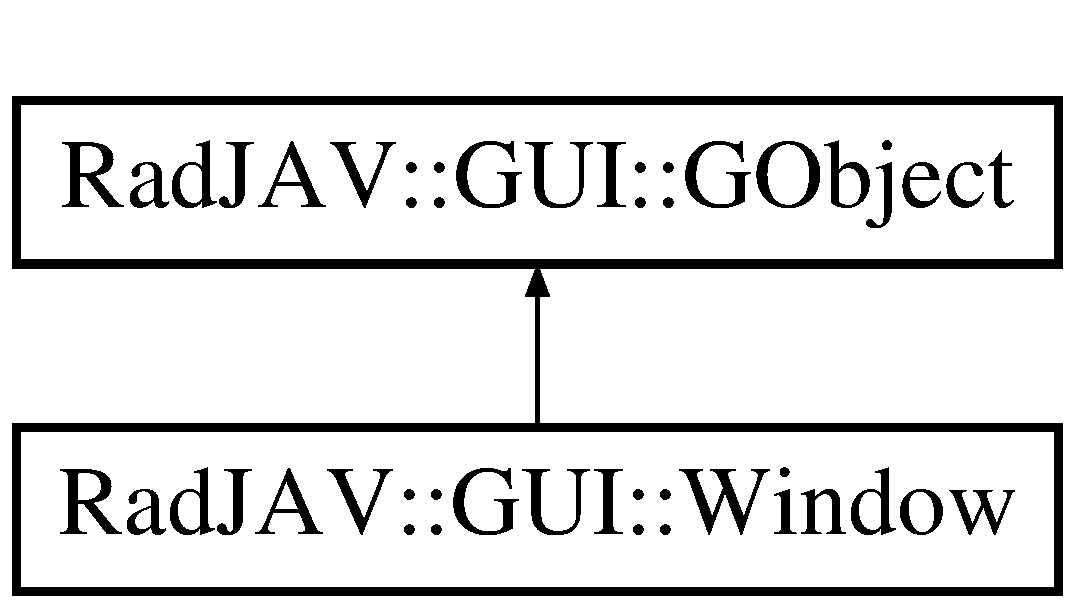
\includegraphics[height=2.000000cm]{class_rad_j_a_v_1_1_g_u_i_1_1_window}
\end{center}
\end{figure}
\subsection*{Public Member Functions}
\begin{DoxyCompactItemize}
\item 
\hyperlink{class_rad_j_a_v_1_1_g_u_i_1_1_window_afe6c5fda53deb03924a3587fdf0a2f21}{Window} (\hyperlink{class_rad_j_a_v_1_1_string}{String} new\+Name)
\item 
\hyperlink{class_rad_j_a_v_1_1_g_u_i_1_1_window_a0ff0dc6d9051251bf5a82f8bd6b7ede1}{Window} (\hyperlink{class_rad_j_a_v_1_1_string}{String} new\+Name, \hyperlink{class_rad_j_a_v_1_1_string}{String} new\+Text)
\item 
\hyperlink{class_rad_j_a_v_1_1_g_u_i_1_1_window_a91fa44be744ead01b131f5e81f14cb7f}{Window} (\hyperlink{class_rad_j_a_v_1_1_string}{String} new\+Name, \hyperlink{class_rad_j_a_v_1_1_string}{String} new\+Text, std\+::shared\+\_\+ptr$<$ \hyperlink{class_rad_j_a_v_1_1_g_u_i_1_1_g_object}{G\+Object} $>$ new\+Parent)
\item 
void \hyperlink{class_rad_j_a_v_1_1_g_u_i_1_1_window_a92bf59c30dd5b9f77d77a31f9a2f8982}{create} ()
\begin{DoxyCompactList}\small\item\em Create the object. \end{DoxyCompactList}\item 
void \hyperlink{class_rad_j_a_v_1_1_g_u_i_1_1_window_acbc9c4caf87c4922bafa4b89dc2a9c03}{set\+Text} (\hyperlink{class_rad_j_a_v_1_1_string}{String} new\+Text)
\begin{DoxyCompactList}\small\item\em Set the object\textquotesingle{}s text. \end{DoxyCompactList}\item 
\hyperlink{class_rad_j_a_v_1_1_string}{String} \hyperlink{class_rad_j_a_v_1_1_g_u_i_1_1_window_a91a0cb7a172dc0ff1e378706b033cf3d}{get\+Text} ()
\begin{DoxyCompactList}\small\item\em Get the object\textquotesingle{}s text. \end{DoxyCompactList}\item 
void \hyperlink{class_rad_j_a_v_1_1_g_u_i_1_1_window_a7e92748e13733aa6c2b15beaaa76ab55}{set\+Visibility} (bool new\+Visible)
\begin{DoxyCompactList}\small\item\em Set the visibility of this object. \end{DoxyCompactList}\item 
bool \hyperlink{class_rad_j_a_v_1_1_g_u_i_1_1_window_a4ddb8d5a94c7fcaadb1bed004c80561b}{get\+Visibility} ()
\begin{DoxyCompactList}\small\item\em Get the visibility of this object. \end{DoxyCompactList}\item 
void \hyperlink{class_rad_j_a_v_1_1_g_u_i_1_1_window_a0b9e73f35922418bd2a6c52d349b8bcf}{on} (\hyperlink{class_rad_j_a_v_1_1_string}{String} event\+Name, std\+::function$<$ void()$>$ func)
\begin{DoxyCompactList}\small\item\em Calls a function when an event is triggered. \end{DoxyCompactList}\end{DoxyCompactItemize}
\subsection*{Additional Inherited Members}


\subsection{Constructor \& Destructor Documentation}
\index{Rad\+J\+A\+V\+::\+G\+U\+I\+::\+Window@{Rad\+J\+A\+V\+::\+G\+U\+I\+::\+Window}!Window@{Window}}
\index{Window@{Window}!Rad\+J\+A\+V\+::\+G\+U\+I\+::\+Window@{Rad\+J\+A\+V\+::\+G\+U\+I\+::\+Window}}
\subsubsection[{\texorpdfstring{Window(\+String new\+Name)}{Window(String newName)}}]{\setlength{\rightskip}{0pt plus 5cm}Rad\+J\+A\+V\+::\+G\+U\+I\+::\+Window\+::\+Window (
\begin{DoxyParamCaption}
\item[{{\bf String}}]{new\+Name}
\end{DoxyParamCaption}
)}\hypertarget{class_rad_j_a_v_1_1_g_u_i_1_1_window_afe6c5fda53deb03924a3587fdf0a2f21}{}\label{class_rad_j_a_v_1_1_g_u_i_1_1_window_afe6c5fda53deb03924a3587fdf0a2f21}
\index{Rad\+J\+A\+V\+::\+G\+U\+I\+::\+Window@{Rad\+J\+A\+V\+::\+G\+U\+I\+::\+Window}!Window@{Window}}
\index{Window@{Window}!Rad\+J\+A\+V\+::\+G\+U\+I\+::\+Window@{Rad\+J\+A\+V\+::\+G\+U\+I\+::\+Window}}
\subsubsection[{\texorpdfstring{Window(\+String new\+Name, String new\+Text)}{Window(String newName, String newText)}}]{\setlength{\rightskip}{0pt plus 5cm}Rad\+J\+A\+V\+::\+G\+U\+I\+::\+Window\+::\+Window (
\begin{DoxyParamCaption}
\item[{{\bf String}}]{new\+Name, }
\item[{{\bf String}}]{new\+Text}
\end{DoxyParamCaption}
)}\hypertarget{class_rad_j_a_v_1_1_g_u_i_1_1_window_a0ff0dc6d9051251bf5a82f8bd6b7ede1}{}\label{class_rad_j_a_v_1_1_g_u_i_1_1_window_a0ff0dc6d9051251bf5a82f8bd6b7ede1}
\index{Rad\+J\+A\+V\+::\+G\+U\+I\+::\+Window@{Rad\+J\+A\+V\+::\+G\+U\+I\+::\+Window}!Window@{Window}}
\index{Window@{Window}!Rad\+J\+A\+V\+::\+G\+U\+I\+::\+Window@{Rad\+J\+A\+V\+::\+G\+U\+I\+::\+Window}}
\subsubsection[{\texorpdfstring{Window(\+String new\+Name, String new\+Text, std\+::shared\+\_\+ptr$<$ G\+Object $>$ new\+Parent)}{Window(String newName, String newText, std::shared_ptr< GObject > newParent)}}]{\setlength{\rightskip}{0pt plus 5cm}Rad\+J\+A\+V\+::\+G\+U\+I\+::\+Window\+::\+Window (
\begin{DoxyParamCaption}
\item[{{\bf String}}]{new\+Name, }
\item[{{\bf String}}]{new\+Text, }
\item[{std\+::shared\+\_\+ptr$<$ {\bf G\+Object} $>$}]{new\+Parent}
\end{DoxyParamCaption}
)}\hypertarget{class_rad_j_a_v_1_1_g_u_i_1_1_window_a91fa44be744ead01b131f5e81f14cb7f}{}\label{class_rad_j_a_v_1_1_g_u_i_1_1_window_a91fa44be744ead01b131f5e81f14cb7f}


\subsection{Member Function Documentation}
\index{Rad\+J\+A\+V\+::\+G\+U\+I\+::\+Window@{Rad\+J\+A\+V\+::\+G\+U\+I\+::\+Window}!create@{create}}
\index{create@{create}!Rad\+J\+A\+V\+::\+G\+U\+I\+::\+Window@{Rad\+J\+A\+V\+::\+G\+U\+I\+::\+Window}}
\subsubsection[{\texorpdfstring{create()}{create()}}]{\setlength{\rightskip}{0pt plus 5cm}void Rad\+J\+A\+V\+::\+G\+U\+I\+::\+Window\+::create (
\begin{DoxyParamCaption}
{}
\end{DoxyParamCaption}
)\hspace{0.3cm}{\ttfamily [virtual]}}\hypertarget{class_rad_j_a_v_1_1_g_u_i_1_1_window_a92bf59c30dd5b9f77d77a31f9a2f8982}{}\label{class_rad_j_a_v_1_1_g_u_i_1_1_window_a92bf59c30dd5b9f77d77a31f9a2f8982}


Create the object. 



Implements \hyperlink{class_rad_j_a_v_1_1_g_u_i_1_1_g_object_a0758b7d4b69fc985c20c8dc680c8464c}{Rad\+J\+A\+V\+::\+G\+U\+I\+::\+G\+Object}.

\index{Rad\+J\+A\+V\+::\+G\+U\+I\+::\+Window@{Rad\+J\+A\+V\+::\+G\+U\+I\+::\+Window}!get\+Text@{get\+Text}}
\index{get\+Text@{get\+Text}!Rad\+J\+A\+V\+::\+G\+U\+I\+::\+Window@{Rad\+J\+A\+V\+::\+G\+U\+I\+::\+Window}}
\subsubsection[{\texorpdfstring{get\+Text()}{getText()}}]{\setlength{\rightskip}{0pt plus 5cm}{\bf String} Rad\+J\+A\+V\+::\+G\+U\+I\+::\+Window\+::get\+Text (
\begin{DoxyParamCaption}
{}
\end{DoxyParamCaption}
)\hspace{0.3cm}{\ttfamily [virtual]}}\hypertarget{class_rad_j_a_v_1_1_g_u_i_1_1_window_a91a0cb7a172dc0ff1e378706b033cf3d}{}\label{class_rad_j_a_v_1_1_g_u_i_1_1_window_a91a0cb7a172dc0ff1e378706b033cf3d}


Get the object\textquotesingle{}s text. 



Implements \hyperlink{class_rad_j_a_v_1_1_g_u_i_1_1_g_object_a623610eb55210a2f88afbdeda31f088e}{Rad\+J\+A\+V\+::\+G\+U\+I\+::\+G\+Object}.

\index{Rad\+J\+A\+V\+::\+G\+U\+I\+::\+Window@{Rad\+J\+A\+V\+::\+G\+U\+I\+::\+Window}!get\+Visibility@{get\+Visibility}}
\index{get\+Visibility@{get\+Visibility}!Rad\+J\+A\+V\+::\+G\+U\+I\+::\+Window@{Rad\+J\+A\+V\+::\+G\+U\+I\+::\+Window}}
\subsubsection[{\texorpdfstring{get\+Visibility()}{getVisibility()}}]{\setlength{\rightskip}{0pt plus 5cm}bool Rad\+J\+A\+V\+::\+G\+U\+I\+::\+Window\+::get\+Visibility (
\begin{DoxyParamCaption}
{}
\end{DoxyParamCaption}
)\hspace{0.3cm}{\ttfamily [virtual]}}\hypertarget{class_rad_j_a_v_1_1_g_u_i_1_1_window_a4ddb8d5a94c7fcaadb1bed004c80561b}{}\label{class_rad_j_a_v_1_1_g_u_i_1_1_window_a4ddb8d5a94c7fcaadb1bed004c80561b}


Get the visibility of this object. 



Implements \hyperlink{class_rad_j_a_v_1_1_g_u_i_1_1_g_object_a9b30394c246dc1cce788c93e48e6e00d}{Rad\+J\+A\+V\+::\+G\+U\+I\+::\+G\+Object}.

\index{Rad\+J\+A\+V\+::\+G\+U\+I\+::\+Window@{Rad\+J\+A\+V\+::\+G\+U\+I\+::\+Window}!on@{on}}
\index{on@{on}!Rad\+J\+A\+V\+::\+G\+U\+I\+::\+Window@{Rad\+J\+A\+V\+::\+G\+U\+I\+::\+Window}}
\subsubsection[{\texorpdfstring{on(\+String event\+Name, std\+::function$<$ void()$>$ func)}{on(String eventName, std::function< void()> func)}}]{\setlength{\rightskip}{0pt plus 5cm}void Rad\+J\+A\+V\+::\+G\+U\+I\+::\+Window\+::on (
\begin{DoxyParamCaption}
\item[{{\bf String}}]{event\+Name, }
\item[{std\+::function$<$ void()$>$}]{func}
\end{DoxyParamCaption}
)\hspace{0.3cm}{\ttfamily [virtual]}}\hypertarget{class_rad_j_a_v_1_1_g_u_i_1_1_window_a0b9e73f35922418bd2a6c52d349b8bcf}{}\label{class_rad_j_a_v_1_1_g_u_i_1_1_window_a0b9e73f35922418bd2a6c52d349b8bcf}


Calls a function when an event is triggered. 



Implements \hyperlink{class_rad_j_a_v_1_1_g_u_i_1_1_g_object_a224cec9275e8e5197d813ac5996f713c}{Rad\+J\+A\+V\+::\+G\+U\+I\+::\+G\+Object}.

\index{Rad\+J\+A\+V\+::\+G\+U\+I\+::\+Window@{Rad\+J\+A\+V\+::\+G\+U\+I\+::\+Window}!set\+Text@{set\+Text}}
\index{set\+Text@{set\+Text}!Rad\+J\+A\+V\+::\+G\+U\+I\+::\+Window@{Rad\+J\+A\+V\+::\+G\+U\+I\+::\+Window}}
\subsubsection[{\texorpdfstring{set\+Text(\+String new\+Text)}{setText(String newText)}}]{\setlength{\rightskip}{0pt plus 5cm}void Rad\+J\+A\+V\+::\+G\+U\+I\+::\+Window\+::set\+Text (
\begin{DoxyParamCaption}
\item[{{\bf String}}]{new\+Text}
\end{DoxyParamCaption}
)\hspace{0.3cm}{\ttfamily [virtual]}}\hypertarget{class_rad_j_a_v_1_1_g_u_i_1_1_window_acbc9c4caf87c4922bafa4b89dc2a9c03}{}\label{class_rad_j_a_v_1_1_g_u_i_1_1_window_acbc9c4caf87c4922bafa4b89dc2a9c03}


Set the object\textquotesingle{}s text. 



Implements \hyperlink{class_rad_j_a_v_1_1_g_u_i_1_1_g_object_a361fe7962341e8d0562b39d28ad1b465}{Rad\+J\+A\+V\+::\+G\+U\+I\+::\+G\+Object}.

\index{Rad\+J\+A\+V\+::\+G\+U\+I\+::\+Window@{Rad\+J\+A\+V\+::\+G\+U\+I\+::\+Window}!set\+Visibility@{set\+Visibility}}
\index{set\+Visibility@{set\+Visibility}!Rad\+J\+A\+V\+::\+G\+U\+I\+::\+Window@{Rad\+J\+A\+V\+::\+G\+U\+I\+::\+Window}}
\subsubsection[{\texorpdfstring{set\+Visibility(bool new\+Visible)}{setVisibility(bool newVisible)}}]{\setlength{\rightskip}{0pt plus 5cm}void Rad\+J\+A\+V\+::\+G\+U\+I\+::\+Window\+::set\+Visibility (
\begin{DoxyParamCaption}
\item[{bool}]{new\+Visible}
\end{DoxyParamCaption}
)\hspace{0.3cm}{\ttfamily [virtual]}}\hypertarget{class_rad_j_a_v_1_1_g_u_i_1_1_window_a7e92748e13733aa6c2b15beaaa76ab55}{}\label{class_rad_j_a_v_1_1_g_u_i_1_1_window_a7e92748e13733aa6c2b15beaaa76ab55}


Set the visibility of this object. 



Implements \hyperlink{class_rad_j_a_v_1_1_g_u_i_1_1_g_object_a108ec023dce72af50ce3bbe5fb61b394}{Rad\+J\+A\+V\+::\+G\+U\+I\+::\+G\+Object}.



The documentation for this class was generated from the following files\+:\begin{DoxyCompactItemize}
\item 
include/\+Rad\+Jav/\hyperlink{_rad_jav_g_u_i_window_8h}{Rad\+Jav\+G\+U\+I\+Window.\+h}\item 
src/\+Rad\+Jav/\hyperlink{_rad_jav_g_u_i_window_8cpp}{Rad\+Jav\+G\+U\+I\+Window.\+cpp}\end{DoxyCompactItemize}

\hypertarget{class_rad_j_a_v_1_1wx_widgets_rad_jav}{}\section{Rad\+J\+AV\+:\+:wx\+Widgets\+Rad\+Jav Class Reference}
\label{class_rad_j_a_v_1_1wx_widgets_rad_jav}\index{Rad\+J\+A\+V\+::wx\+Widgets\+Rad\+Jav@{Rad\+J\+A\+V\+::wx\+Widgets\+Rad\+Jav}}


wx\+Widgets for \mbox{\hyperlink{class_rad_j_a_v_1_1_rad_jav}{Rad\+Jav}}  




{\ttfamily \#include $<$Rad\+Jav\+Wx\+Widgets.\+h$>$}

Inheritance diagram for Rad\+J\+AV\+:\+:wx\+Widgets\+Rad\+Jav\+:\begin{figure}[H]
\begin{center}
\leavevmode
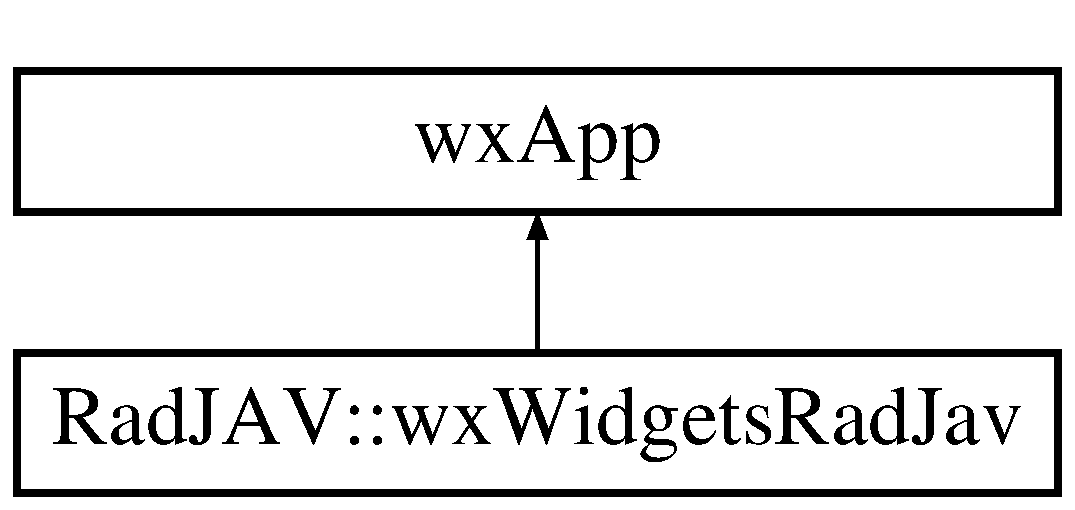
\includegraphics[height=2.000000cm]{class_rad_j_a_v_1_1wx_widgets_rad_jav}
\end{center}
\end{figure}
\subsection*{Public Member Functions}
\begin{DoxyCompactItemize}
\item 
\mbox{\hyperlink{class_rad_j_a_v_1_1wx_widgets_rad_jav_a81ff56b4ae9e9d4c50155151eadc35b7}{wx\+Widgets\+Rad\+Jav}} ()
\item 
bool \mbox{\hyperlink{class_rad_j_a_v_1_1wx_widgets_rad_jav_a9e8269312d40feafc94718a0b2912de8}{On\+Init}} ()
\begin{DoxyCompactList}\small\item\em Executes when the app has initialized. \end{DoxyCompactList}\item 
int \mbox{\hyperlink{class_rad_j_a_v_1_1wx_widgets_rad_jav_a37c46a1705f10f3bd0a79fa148361400}{On\+Run}} ()
\item 
void \mbox{\hyperlink{class_rad_j_a_v_1_1wx_widgets_rad_jav_a8fc014edbdcd68cc1ad849fe148f9871}{On\+Unhandled\+Exception}} ()
\item 
void \mbox{\hyperlink{class_rad_j_a_v_1_1wx_widgets_rad_jav_ad73346ef2ddf9aa8855bf07c349519cb}{On\+Fatal\+Exception}} ()
\item 
int \mbox{\hyperlink{class_rad_j_a_v_1_1wx_widgets_rad_jav_add7d79813e2e017382a8a9da399e91ce}{On\+Exit}} ()
\item 
void \mbox{\hyperlink{class_rad_j_a_v_1_1wx_widgets_rad_jav_ad96e50771b485673fbefaf9bb102441d}{Server\+Event}} (wx\+Socket\+Event \&evt\+Event)
\item 
void \mbox{\hyperlink{class_rad_j_a_v_1_1wx_widgets_rad_jav_a2bf79b1939cb6f8239e6a5144701fa6d}{Socket\+Event}} (wx\+Socket\+Event \&evt\+Event)
\item 
void \mbox{\hyperlink{class_rad_j_a_v_1_1wx_widgets_rad_jav_aefe213408c6f7fb404d5a8a270e9b7d7}{run\+System}} ()
\end{DoxyCompactItemize}
\subsection*{Public Attributes}
\begin{DoxyCompactItemize}
\item 
\mbox{\hyperlink{class_rad_j_a_v_1_1_array}{Array}}$<$ wx\+Thread $\ast$ $>$ \mbox{\hyperlink{class_rad_j_a_v_1_1wx_widgets_rad_jav_a5fca84f30363bbe567c2c3c020fad9a4}{ary\+Threads}}
\item 
wx\+Critical\+Section \mbox{\hyperlink{class_rad_j_a_v_1_1wx_widgets_rad_jav_a93753443d9f01ad987a127cf496ba39e}{wcs\+Critical}}
\end{DoxyCompactItemize}


\subsection{Detailed Description}
wx\+Widgets for \mbox{\hyperlink{class_rad_j_a_v_1_1_rad_jav}{Rad\+Jav}} 

\subsection{Constructor \& Destructor Documentation}
\mbox{\Hypertarget{class_rad_j_a_v_1_1wx_widgets_rad_jav_a81ff56b4ae9e9d4c50155151eadc35b7}\label{class_rad_j_a_v_1_1wx_widgets_rad_jav_a81ff56b4ae9e9d4c50155151eadc35b7}} 
\index{Rad\+J\+A\+V\+::wx\+Widgets\+Rad\+Jav@{Rad\+J\+A\+V\+::wx\+Widgets\+Rad\+Jav}!wx\+Widgets\+Rad\+Jav@{wx\+Widgets\+Rad\+Jav}}
\index{wx\+Widgets\+Rad\+Jav@{wx\+Widgets\+Rad\+Jav}!Rad\+J\+A\+V\+::wx\+Widgets\+Rad\+Jav@{Rad\+J\+A\+V\+::wx\+Widgets\+Rad\+Jav}}
\subsubsection{\texorpdfstring{wx\+Widgets\+Rad\+Jav()}{wxWidgetsRadJav()}}
{\footnotesize\ttfamily Rad\+J\+A\+V\+::wx\+Widgets\+Rad\+Jav\+::wx\+Widgets\+Rad\+Jav (\begin{DoxyParamCaption}{ }\end{DoxyParamCaption})\hspace{0.3cm}{\ttfamily [inline]}}



\subsection{Member Function Documentation}
\mbox{\Hypertarget{class_rad_j_a_v_1_1wx_widgets_rad_jav_add7d79813e2e017382a8a9da399e91ce}\label{class_rad_j_a_v_1_1wx_widgets_rad_jav_add7d79813e2e017382a8a9da399e91ce}} 
\index{Rad\+J\+A\+V\+::wx\+Widgets\+Rad\+Jav@{Rad\+J\+A\+V\+::wx\+Widgets\+Rad\+Jav}!On\+Exit@{On\+Exit}}
\index{On\+Exit@{On\+Exit}!Rad\+J\+A\+V\+::wx\+Widgets\+Rad\+Jav@{Rad\+J\+A\+V\+::wx\+Widgets\+Rad\+Jav}}
\subsubsection{\texorpdfstring{On\+Exit()}{OnExit()}}
{\footnotesize\ttfamily int Rad\+J\+A\+V\+::wx\+Widgets\+Rad\+Jav\+::\+On\+Exit (\begin{DoxyParamCaption}{ }\end{DoxyParamCaption})}

\mbox{\Hypertarget{class_rad_j_a_v_1_1wx_widgets_rad_jav_ad73346ef2ddf9aa8855bf07c349519cb}\label{class_rad_j_a_v_1_1wx_widgets_rad_jav_ad73346ef2ddf9aa8855bf07c349519cb}} 
\index{Rad\+J\+A\+V\+::wx\+Widgets\+Rad\+Jav@{Rad\+J\+A\+V\+::wx\+Widgets\+Rad\+Jav}!On\+Fatal\+Exception@{On\+Fatal\+Exception}}
\index{On\+Fatal\+Exception@{On\+Fatal\+Exception}!Rad\+J\+A\+V\+::wx\+Widgets\+Rad\+Jav@{Rad\+J\+A\+V\+::wx\+Widgets\+Rad\+Jav}}
\subsubsection{\texorpdfstring{On\+Fatal\+Exception()}{OnFatalException()}}
{\footnotesize\ttfamily void Rad\+J\+A\+V\+::wx\+Widgets\+Rad\+Jav\+::\+On\+Fatal\+Exception (\begin{DoxyParamCaption}{ }\end{DoxyParamCaption})}

\mbox{\Hypertarget{class_rad_j_a_v_1_1wx_widgets_rad_jav_a9e8269312d40feafc94718a0b2912de8}\label{class_rad_j_a_v_1_1wx_widgets_rad_jav_a9e8269312d40feafc94718a0b2912de8}} 
\index{Rad\+J\+A\+V\+::wx\+Widgets\+Rad\+Jav@{Rad\+J\+A\+V\+::wx\+Widgets\+Rad\+Jav}!On\+Init@{On\+Init}}
\index{On\+Init@{On\+Init}!Rad\+J\+A\+V\+::wx\+Widgets\+Rad\+Jav@{Rad\+J\+A\+V\+::wx\+Widgets\+Rad\+Jav}}
\subsubsection{\texorpdfstring{On\+Init()}{OnInit()}}
{\footnotesize\ttfamily bool Rad\+J\+A\+V\+::wx\+Widgets\+Rad\+Jav\+::\+On\+Init (\begin{DoxyParamCaption}{ }\end{DoxyParamCaption})}



Executes when the app has initialized. 

\mbox{\Hypertarget{class_rad_j_a_v_1_1wx_widgets_rad_jav_a37c46a1705f10f3bd0a79fa148361400}\label{class_rad_j_a_v_1_1wx_widgets_rad_jav_a37c46a1705f10f3bd0a79fa148361400}} 
\index{Rad\+J\+A\+V\+::wx\+Widgets\+Rad\+Jav@{Rad\+J\+A\+V\+::wx\+Widgets\+Rad\+Jav}!On\+Run@{On\+Run}}
\index{On\+Run@{On\+Run}!Rad\+J\+A\+V\+::wx\+Widgets\+Rad\+Jav@{Rad\+J\+A\+V\+::wx\+Widgets\+Rad\+Jav}}
\subsubsection{\texorpdfstring{On\+Run()}{OnRun()}}
{\footnotesize\ttfamily int Rad\+J\+A\+V\+::wx\+Widgets\+Rad\+Jav\+::\+On\+Run (\begin{DoxyParamCaption}{ }\end{DoxyParamCaption})}

\mbox{\Hypertarget{class_rad_j_a_v_1_1wx_widgets_rad_jav_a8fc014edbdcd68cc1ad849fe148f9871}\label{class_rad_j_a_v_1_1wx_widgets_rad_jav_a8fc014edbdcd68cc1ad849fe148f9871}} 
\index{Rad\+J\+A\+V\+::wx\+Widgets\+Rad\+Jav@{Rad\+J\+A\+V\+::wx\+Widgets\+Rad\+Jav}!On\+Unhandled\+Exception@{On\+Unhandled\+Exception}}
\index{On\+Unhandled\+Exception@{On\+Unhandled\+Exception}!Rad\+J\+A\+V\+::wx\+Widgets\+Rad\+Jav@{Rad\+J\+A\+V\+::wx\+Widgets\+Rad\+Jav}}
\subsubsection{\texorpdfstring{On\+Unhandled\+Exception()}{OnUnhandledException()}}
{\footnotesize\ttfamily void Rad\+J\+A\+V\+::wx\+Widgets\+Rad\+Jav\+::\+On\+Unhandled\+Exception (\begin{DoxyParamCaption}{ }\end{DoxyParamCaption})}

\mbox{\Hypertarget{class_rad_j_a_v_1_1wx_widgets_rad_jav_aefe213408c6f7fb404d5a8a270e9b7d7}\label{class_rad_j_a_v_1_1wx_widgets_rad_jav_aefe213408c6f7fb404d5a8a270e9b7d7}} 
\index{Rad\+J\+A\+V\+::wx\+Widgets\+Rad\+Jav@{Rad\+J\+A\+V\+::wx\+Widgets\+Rad\+Jav}!run\+System@{run\+System}}
\index{run\+System@{run\+System}!Rad\+J\+A\+V\+::wx\+Widgets\+Rad\+Jav@{Rad\+J\+A\+V\+::wx\+Widgets\+Rad\+Jav}}
\subsubsection{\texorpdfstring{run\+System()}{runSystem()}}
{\footnotesize\ttfamily void Rad\+J\+A\+V\+::wx\+Widgets\+Rad\+Jav\+::run\+System (\begin{DoxyParamCaption}{ }\end{DoxyParamCaption})}

\mbox{\Hypertarget{class_rad_j_a_v_1_1wx_widgets_rad_jav_ad96e50771b485673fbefaf9bb102441d}\label{class_rad_j_a_v_1_1wx_widgets_rad_jav_ad96e50771b485673fbefaf9bb102441d}} 
\index{Rad\+J\+A\+V\+::wx\+Widgets\+Rad\+Jav@{Rad\+J\+A\+V\+::wx\+Widgets\+Rad\+Jav}!Server\+Event@{Server\+Event}}
\index{Server\+Event@{Server\+Event}!Rad\+J\+A\+V\+::wx\+Widgets\+Rad\+Jav@{Rad\+J\+A\+V\+::wx\+Widgets\+Rad\+Jav}}
\subsubsection{\texorpdfstring{Server\+Event()}{ServerEvent()}}
{\footnotesize\ttfamily void Rad\+J\+A\+V\+::wx\+Widgets\+Rad\+Jav\+::\+Server\+Event (\begin{DoxyParamCaption}\item[{wx\+Socket\+Event \&}]{evt\+Event }\end{DoxyParamCaption})}

\mbox{\Hypertarget{class_rad_j_a_v_1_1wx_widgets_rad_jav_a2bf79b1939cb6f8239e6a5144701fa6d}\label{class_rad_j_a_v_1_1wx_widgets_rad_jav_a2bf79b1939cb6f8239e6a5144701fa6d}} 
\index{Rad\+J\+A\+V\+::wx\+Widgets\+Rad\+Jav@{Rad\+J\+A\+V\+::wx\+Widgets\+Rad\+Jav}!Socket\+Event@{Socket\+Event}}
\index{Socket\+Event@{Socket\+Event}!Rad\+J\+A\+V\+::wx\+Widgets\+Rad\+Jav@{Rad\+J\+A\+V\+::wx\+Widgets\+Rad\+Jav}}
\subsubsection{\texorpdfstring{Socket\+Event()}{SocketEvent()}}
{\footnotesize\ttfamily void Rad\+J\+A\+V\+::wx\+Widgets\+Rad\+Jav\+::\+Socket\+Event (\begin{DoxyParamCaption}\item[{wx\+Socket\+Event \&}]{evt\+Event }\end{DoxyParamCaption})}



\subsection{Member Data Documentation}
\mbox{\Hypertarget{class_rad_j_a_v_1_1wx_widgets_rad_jav_a5fca84f30363bbe567c2c3c020fad9a4}\label{class_rad_j_a_v_1_1wx_widgets_rad_jav_a5fca84f30363bbe567c2c3c020fad9a4}} 
\index{Rad\+J\+A\+V\+::wx\+Widgets\+Rad\+Jav@{Rad\+J\+A\+V\+::wx\+Widgets\+Rad\+Jav}!ary\+Threads@{ary\+Threads}}
\index{ary\+Threads@{ary\+Threads}!Rad\+J\+A\+V\+::wx\+Widgets\+Rad\+Jav@{Rad\+J\+A\+V\+::wx\+Widgets\+Rad\+Jav}}
\subsubsection{\texorpdfstring{ary\+Threads}{aryThreads}}
{\footnotesize\ttfamily \mbox{\hyperlink{class_rad_j_a_v_1_1_array}{Array}}$<$wx\+Thread $\ast$$>$ Rad\+J\+A\+V\+::wx\+Widgets\+Rad\+Jav\+::ary\+Threads}

\mbox{\Hypertarget{class_rad_j_a_v_1_1wx_widgets_rad_jav_a93753443d9f01ad987a127cf496ba39e}\label{class_rad_j_a_v_1_1wx_widgets_rad_jav_a93753443d9f01ad987a127cf496ba39e}} 
\index{Rad\+J\+A\+V\+::wx\+Widgets\+Rad\+Jav@{Rad\+J\+A\+V\+::wx\+Widgets\+Rad\+Jav}!wcs\+Critical@{wcs\+Critical}}
\index{wcs\+Critical@{wcs\+Critical}!Rad\+J\+A\+V\+::wx\+Widgets\+Rad\+Jav@{Rad\+J\+A\+V\+::wx\+Widgets\+Rad\+Jav}}
\subsubsection{\texorpdfstring{wcs\+Critical}{wcsCritical}}
{\footnotesize\ttfamily wx\+Critical\+Section Rad\+J\+A\+V\+::wx\+Widgets\+Rad\+Jav\+::wcs\+Critical}



The documentation for this class was generated from the following file\+:\begin{DoxyCompactItemize}
\item 
include/\+Rad\+Jav/\mbox{\hyperlink{_rad_jav_wx_widgets_8h}{Rad\+Jav\+Wx\+Widgets.\+h}}\end{DoxyCompactItemize}

\hypertarget{class_rad_j_a_v_1_1_networking_1_1wx_widgets_t_c_p_client}{}\section{Rad\+J\+AV\+:\+:Networking\+:\+:wx\+Widgets\+T\+C\+P\+Client Class Reference}
\label{class_rad_j_a_v_1_1_networking_1_1wx_widgets_t_c_p_client}\index{Rad\+J\+A\+V\+::\+Networking\+::wx\+Widgets\+T\+C\+P\+Client@{Rad\+J\+A\+V\+::\+Networking\+::wx\+Widgets\+T\+C\+P\+Client}}


{\ttfamily \#include $<$Rad\+Jav\+Wx\+Widgets\+Networking.\+h$>$}

Inheritance diagram for Rad\+J\+AV\+:\+:Networking\+:\+:wx\+Widgets\+T\+C\+P\+Client\+:\begin{figure}[H]
\begin{center}
\leavevmode
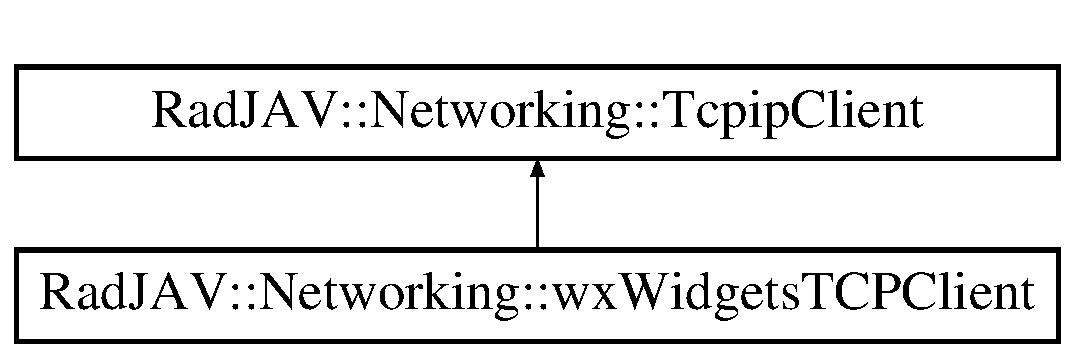
\includegraphics[height=2.000000cm]{class_rad_j_a_v_1_1_networking_1_1wx_widgets_t_c_p_client}
\end{center}
\end{figure}
\subsection*{Public Member Functions}
\begin{DoxyCompactItemize}
\item 
\mbox{\hyperlink{class_rad_j_a_v_1_1_networking_1_1wx_widgets_t_c_p_client_af80442d38749a9cd12a45ef7d8f7928c}{wx\+Widgets\+T\+C\+P\+Client}} ()
\item 
bool \mbox{\hyperlink{class_rad_j_a_v_1_1_networking_1_1wx_widgets_t_c_p_client_aee6ffb935babab8f984e3edd6ab100cd}{Init}} (unsigned short us\+Port\+Pass)
\item 
bool \mbox{\hyperlink{class_rad_j_a_v_1_1_networking_1_1wx_widgets_t_c_p_client_a92d5158fc70110d7c152d32382418640}{Connect\+With\+Blocking}} (\mbox{\hyperlink{class_rad_j_a_v_1_1_string}{String}} str\+Connect\+To)
\item 
bool \mbox{\hyperlink{class_rad_j_a_v_1_1_networking_1_1wx_widgets_t_c_p_client_a2aebbf48ef53705babf0f4914cc8e23e}{Connect\+Without\+Blocking}} (\mbox{\hyperlink{class_rad_j_a_v_1_1_string}{String}} str\+Connect\+To)
\item 
bool \mbox{\hyperlink{class_rad_j_a_v_1_1_networking_1_1wx_widgets_t_c_p_client_ad683dafeb275ab9b1dd60bcd1f177107}{send\+Float}} (float f\+Float)
\begin{DoxyCompactList}\small\item\em Send a float to the server. \end{DoxyCompactList}\item 
bool \mbox{\hyperlink{class_rad_j_a_v_1_1_networking_1_1wx_widgets_t_c_p_client_afb57ef92f150833532015d14475a5ae1}{send\+Double}} (double d\+Double)
\begin{DoxyCompactList}\small\item\em Send a double to the server. \end{DoxyCompactList}\item 
bool \mbox{\hyperlink{class_rad_j_a_v_1_1_networking_1_1wx_widgets_t_c_p_client_a8463c6778160ef13bfd87dac47676614}{send\+Int}} (int i\+Int)
\begin{DoxyCompactList}\small\item\em Send an int to the server. \end{DoxyCompactList}\item 
bool \mbox{\hyperlink{class_rad_j_a_v_1_1_networking_1_1wx_widgets_t_c_p_client_a548db141df3e65127f8a96dbfe63cea1}{send\+U\+Int}} (size\+\_\+t ui\+Int)
\begin{DoxyCompactList}\small\item\em Send an size\+\_\+t to the server. \end{DoxyCompactList}\item 
bool \mbox{\hyperlink{class_rad_j_a_v_1_1_networking_1_1wx_widgets_t_c_p_client_aaa40b254965bfc2b4d3b27877602da9c}{send\+Long}} (long l\+Long)
\begin{DoxyCompactList}\small\item\em Send a long to the server. \end{DoxyCompactList}\item 
bool \mbox{\hyperlink{class_rad_j_a_v_1_1_networking_1_1wx_widgets_t_c_p_client_a8440ad8c4446f1525329cfe40d630ead}{send\+U\+Long}} (unsigned long ul\+Long)
\begin{DoxyCompactList}\small\item\em Send an unsigned long to the server. \end{DoxyCompactList}\item 
bool \mbox{\hyperlink{class_rad_j_a_v_1_1_networking_1_1wx_widgets_t_c_p_client_afeb26d6478b3c8f869f67c41e3105bec}{send\+Short}} (short s\+Short)
\begin{DoxyCompactList}\small\item\em Send a short to the server. \end{DoxyCompactList}\item 
bool \mbox{\hyperlink{class_rad_j_a_v_1_1_networking_1_1wx_widgets_t_c_p_client_a909ddced28c91178cfc77be15e79751d}{send\+U\+Short}} (unsigned short us\+Short)
\begin{DoxyCompactList}\small\item\em Send an unsigned short to the server. \end{DoxyCompactList}\item 
bool \mbox{\hyperlink{class_rad_j_a_v_1_1_networking_1_1wx_widgets_t_c_p_client_a3fdaa69183625a5555d99da0a32c6700}{send\+Char}} (char c\+Char)
\begin{DoxyCompactList}\small\item\em Send a char to the server. \end{DoxyCompactList}\item 
bool \mbox{\hyperlink{class_rad_j_a_v_1_1_networking_1_1wx_widgets_t_c_p_client_ae50f5c377cd8116159f7afa5e7f0bbd5}{send\+U\+Char}} (unsigned char uc\+Char)
\begin{DoxyCompactList}\small\item\em Send an unsigned char to the server. \end{DoxyCompactList}\item 
bool \mbox{\hyperlink{class_rad_j_a_v_1_1_networking_1_1wx_widgets_t_c_p_client_a2282375d71da7b7d38ef06a977e46827}{send\+String}} (\mbox{\hyperlink{class_rad_j_a_v_1_1_string}{String}} str\+Line)
\begin{DoxyCompactList}\small\item\em Send a string to the server. \end{DoxyCompactList}\item 
float \mbox{\hyperlink{class_rad_j_a_v_1_1_networking_1_1wx_widgets_t_c_p_client_accbbc7a429265395c0aaa0e55120ab36}{Recv\+Float}} ()
\item 
double \mbox{\hyperlink{class_rad_j_a_v_1_1_networking_1_1wx_widgets_t_c_p_client_a5fe45956f526465748febd1dfbf1a738}{Recv\+Double}} ()
\item 
int \mbox{\hyperlink{class_rad_j_a_v_1_1_networking_1_1wx_widgets_t_c_p_client_ad80311f3c9bfb5e6d3f432b4227bc65a}{Recv\+Int}} ()
\item 
size\+\_\+t \mbox{\hyperlink{class_rad_j_a_v_1_1_networking_1_1wx_widgets_t_c_p_client_ade7a4048aacdfac8a29b0936e1c87749}{Recv\+U\+Int}} ()
\item 
long \mbox{\hyperlink{class_rad_j_a_v_1_1_networking_1_1wx_widgets_t_c_p_client_a33ec446384ae86b928dfd92793f671af}{Recv\+Long}} ()
\item 
unsigned long \mbox{\hyperlink{class_rad_j_a_v_1_1_networking_1_1wx_widgets_t_c_p_client_a1ccd980056060e875f5cc680c91732e6}{Recv\+U\+Long}} ()
\item 
short \mbox{\hyperlink{class_rad_j_a_v_1_1_networking_1_1wx_widgets_t_c_p_client_a13eee779bf8281cadfa24f927dc02158}{Recv\+Short}} ()
\item 
unsigned short \mbox{\hyperlink{class_rad_j_a_v_1_1_networking_1_1wx_widgets_t_c_p_client_a80e785e8bf0473ab47f1dc906f0ac0b1}{Recv\+U\+Short}} ()
\item 
char \mbox{\hyperlink{class_rad_j_a_v_1_1_networking_1_1wx_widgets_t_c_p_client_a2c2ec4d4c31f46ad085ba5bde8645a53}{Recv\+Char}} ()
\item 
unsigned char \mbox{\hyperlink{class_rad_j_a_v_1_1_networking_1_1wx_widgets_t_c_p_client_a3b212a49fa6e35f2b15c7ed58b53188d}{Recv\+U\+Char}} ()
\item 
char $\ast$ \mbox{\hyperlink{class_rad_j_a_v_1_1_networking_1_1wx_widgets_t_c_p_client_a6bce2ed1b76426bbdc7fddc1c676fe57}{Recv\+String}} (int i\+Length)
\item 
\mbox{\hyperlink{class_rad_j_a_v_1_1_string}{String}} \mbox{\hyperlink{class_rad_j_a_v_1_1_networking_1_1wx_widgets_t_c_p_client_abd7b224de561ac1a90d1677df5243952}{Recv\+String}} ()
\item 
void \mbox{\hyperlink{class_rad_j_a_v_1_1_networking_1_1wx_widgets_t_c_p_client_a7a5b908897319073f06fac0a70859ce8}{Set\+Port}} (unsigned short us\+Port\+Pass)
\item 
unsigned short \mbox{\hyperlink{class_rad_j_a_v_1_1_networking_1_1wx_widgets_t_c_p_client_a1b51e3638dc1cefcad9926b38e6e1fdb}{Get\+Port}} ()
\item 
void \mbox{\hyperlink{class_rad_j_a_v_1_1_networking_1_1wx_widgets_t_c_p_client_aeb23b2c93b6be3edb631cc47778ffc84}{Set\+Socket}} (wx\+Socket\+Client $\ast$soc\+Socket\+Pass)
\item 
wx\+Socket\+Client $\ast$ \mbox{\hyperlink{class_rad_j_a_v_1_1_networking_1_1wx_widgets_t_c_p_client_a89808fa1a512f020412427d22eb6af8e}{Get\+Socket}} ()
\item 
\mbox{\hyperlink{class_rad_j_a_v_1_1_string}{String}} \mbox{\hyperlink{class_rad_j_a_v_1_1_networking_1_1wx_widgets_t_c_p_client_a6b5ffa78a073659879d3ce2a60e4b1c7}{Get\+Server\+IP}} ()
\item 
\mbox{\hyperlink{class_rad_j_a_v_1_1_string}{String}} \mbox{\hyperlink{class_rad_j_a_v_1_1_networking_1_1wx_widgets_t_c_p_client_a0addc1f9cd997cf6357fe5e655ba40a9}{Get\+Last\+Error}} ()
\item 
bool \mbox{\hyperlink{class_rad_j_a_v_1_1_networking_1_1wx_widgets_t_c_p_client_a6a9a078dcbb3083eae6398e374fb8aa6}{Close}} ()
\end{DoxyCompactItemize}


\subsection{Constructor \& Destructor Documentation}
\mbox{\Hypertarget{class_rad_j_a_v_1_1_networking_1_1wx_widgets_t_c_p_client_af80442d38749a9cd12a45ef7d8f7928c}\label{class_rad_j_a_v_1_1_networking_1_1wx_widgets_t_c_p_client_af80442d38749a9cd12a45ef7d8f7928c}} 
\index{Rad\+J\+A\+V\+::\+Networking\+::wx\+Widgets\+T\+C\+P\+Client@{Rad\+J\+A\+V\+::\+Networking\+::wx\+Widgets\+T\+C\+P\+Client}!wx\+Widgets\+T\+C\+P\+Client@{wx\+Widgets\+T\+C\+P\+Client}}
\index{wx\+Widgets\+T\+C\+P\+Client@{wx\+Widgets\+T\+C\+P\+Client}!Rad\+J\+A\+V\+::\+Networking\+::wx\+Widgets\+T\+C\+P\+Client@{Rad\+J\+A\+V\+::\+Networking\+::wx\+Widgets\+T\+C\+P\+Client}}
\subsubsection{\texorpdfstring{wx\+Widgets\+T\+C\+P\+Client()}{wxWidgetsTCPClient()}}
{\footnotesize\ttfamily Rad\+J\+A\+V\+::\+Networking\+::wx\+Widgets\+T\+C\+P\+Client\+::wx\+Widgets\+T\+C\+P\+Client (\begin{DoxyParamCaption}{ }\end{DoxyParamCaption})}



\subsection{Member Function Documentation}
\mbox{\Hypertarget{class_rad_j_a_v_1_1_networking_1_1wx_widgets_t_c_p_client_a6a9a078dcbb3083eae6398e374fb8aa6}\label{class_rad_j_a_v_1_1_networking_1_1wx_widgets_t_c_p_client_a6a9a078dcbb3083eae6398e374fb8aa6}} 
\index{Rad\+J\+A\+V\+::\+Networking\+::wx\+Widgets\+T\+C\+P\+Client@{Rad\+J\+A\+V\+::\+Networking\+::wx\+Widgets\+T\+C\+P\+Client}!Close@{Close}}
\index{Close@{Close}!Rad\+J\+A\+V\+::\+Networking\+::wx\+Widgets\+T\+C\+P\+Client@{Rad\+J\+A\+V\+::\+Networking\+::wx\+Widgets\+T\+C\+P\+Client}}
\subsubsection{\texorpdfstring{Close()}{Close()}}
{\footnotesize\ttfamily bool Rad\+J\+A\+V\+::\+Networking\+::wx\+Widgets\+T\+C\+P\+Client\+::\+Close (\begin{DoxyParamCaption}{ }\end{DoxyParamCaption})}

\mbox{\Hypertarget{class_rad_j_a_v_1_1_networking_1_1wx_widgets_t_c_p_client_a92d5158fc70110d7c152d32382418640}\label{class_rad_j_a_v_1_1_networking_1_1wx_widgets_t_c_p_client_a92d5158fc70110d7c152d32382418640}} 
\index{Rad\+J\+A\+V\+::\+Networking\+::wx\+Widgets\+T\+C\+P\+Client@{Rad\+J\+A\+V\+::\+Networking\+::wx\+Widgets\+T\+C\+P\+Client}!Connect\+With\+Blocking@{Connect\+With\+Blocking}}
\index{Connect\+With\+Blocking@{Connect\+With\+Blocking}!Rad\+J\+A\+V\+::\+Networking\+::wx\+Widgets\+T\+C\+P\+Client@{Rad\+J\+A\+V\+::\+Networking\+::wx\+Widgets\+T\+C\+P\+Client}}
\subsubsection{\texorpdfstring{Connect\+With\+Blocking()}{ConnectWithBlocking()}}
{\footnotesize\ttfamily bool Rad\+J\+A\+V\+::\+Networking\+::wx\+Widgets\+T\+C\+P\+Client\+::\+Connect\+With\+Blocking (\begin{DoxyParamCaption}\item[{\mbox{\hyperlink{class_rad_j_a_v_1_1_string}{String}}}]{str\+Connect\+To }\end{DoxyParamCaption})}

\mbox{\Hypertarget{class_rad_j_a_v_1_1_networking_1_1wx_widgets_t_c_p_client_a2aebbf48ef53705babf0f4914cc8e23e}\label{class_rad_j_a_v_1_1_networking_1_1wx_widgets_t_c_p_client_a2aebbf48ef53705babf0f4914cc8e23e}} 
\index{Rad\+J\+A\+V\+::\+Networking\+::wx\+Widgets\+T\+C\+P\+Client@{Rad\+J\+A\+V\+::\+Networking\+::wx\+Widgets\+T\+C\+P\+Client}!Connect\+Without\+Blocking@{Connect\+Without\+Blocking}}
\index{Connect\+Without\+Blocking@{Connect\+Without\+Blocking}!Rad\+J\+A\+V\+::\+Networking\+::wx\+Widgets\+T\+C\+P\+Client@{Rad\+J\+A\+V\+::\+Networking\+::wx\+Widgets\+T\+C\+P\+Client}}
\subsubsection{\texorpdfstring{Connect\+Without\+Blocking()}{ConnectWithoutBlocking()}}
{\footnotesize\ttfamily bool Rad\+J\+A\+V\+::\+Networking\+::wx\+Widgets\+T\+C\+P\+Client\+::\+Connect\+Without\+Blocking (\begin{DoxyParamCaption}\item[{\mbox{\hyperlink{class_rad_j_a_v_1_1_string}{String}}}]{str\+Connect\+To }\end{DoxyParamCaption})}

\mbox{\Hypertarget{class_rad_j_a_v_1_1_networking_1_1wx_widgets_t_c_p_client_a0addc1f9cd997cf6357fe5e655ba40a9}\label{class_rad_j_a_v_1_1_networking_1_1wx_widgets_t_c_p_client_a0addc1f9cd997cf6357fe5e655ba40a9}} 
\index{Rad\+J\+A\+V\+::\+Networking\+::wx\+Widgets\+T\+C\+P\+Client@{Rad\+J\+A\+V\+::\+Networking\+::wx\+Widgets\+T\+C\+P\+Client}!Get\+Last\+Error@{Get\+Last\+Error}}
\index{Get\+Last\+Error@{Get\+Last\+Error}!Rad\+J\+A\+V\+::\+Networking\+::wx\+Widgets\+T\+C\+P\+Client@{Rad\+J\+A\+V\+::\+Networking\+::wx\+Widgets\+T\+C\+P\+Client}}
\subsubsection{\texorpdfstring{Get\+Last\+Error()}{GetLastError()}}
{\footnotesize\ttfamily \mbox{\hyperlink{class_rad_j_a_v_1_1_string}{String}} Rad\+J\+A\+V\+::\+Networking\+::wx\+Widgets\+T\+C\+P\+Client\+::\+Get\+Last\+Error (\begin{DoxyParamCaption}{ }\end{DoxyParamCaption})}

\mbox{\Hypertarget{class_rad_j_a_v_1_1_networking_1_1wx_widgets_t_c_p_client_a1b51e3638dc1cefcad9926b38e6e1fdb}\label{class_rad_j_a_v_1_1_networking_1_1wx_widgets_t_c_p_client_a1b51e3638dc1cefcad9926b38e6e1fdb}} 
\index{Rad\+J\+A\+V\+::\+Networking\+::wx\+Widgets\+T\+C\+P\+Client@{Rad\+J\+A\+V\+::\+Networking\+::wx\+Widgets\+T\+C\+P\+Client}!Get\+Port@{Get\+Port}}
\index{Get\+Port@{Get\+Port}!Rad\+J\+A\+V\+::\+Networking\+::wx\+Widgets\+T\+C\+P\+Client@{Rad\+J\+A\+V\+::\+Networking\+::wx\+Widgets\+T\+C\+P\+Client}}
\subsubsection{\texorpdfstring{Get\+Port()}{GetPort()}}
{\footnotesize\ttfamily unsigned short Rad\+J\+A\+V\+::\+Networking\+::wx\+Widgets\+T\+C\+P\+Client\+::\+Get\+Port (\begin{DoxyParamCaption}{ }\end{DoxyParamCaption})}

\mbox{\Hypertarget{class_rad_j_a_v_1_1_networking_1_1wx_widgets_t_c_p_client_a6b5ffa78a073659879d3ce2a60e4b1c7}\label{class_rad_j_a_v_1_1_networking_1_1wx_widgets_t_c_p_client_a6b5ffa78a073659879d3ce2a60e4b1c7}} 
\index{Rad\+J\+A\+V\+::\+Networking\+::wx\+Widgets\+T\+C\+P\+Client@{Rad\+J\+A\+V\+::\+Networking\+::wx\+Widgets\+T\+C\+P\+Client}!Get\+Server\+IP@{Get\+Server\+IP}}
\index{Get\+Server\+IP@{Get\+Server\+IP}!Rad\+J\+A\+V\+::\+Networking\+::wx\+Widgets\+T\+C\+P\+Client@{Rad\+J\+A\+V\+::\+Networking\+::wx\+Widgets\+T\+C\+P\+Client}}
\subsubsection{\texorpdfstring{Get\+Server\+I\+P()}{GetServerIP()}}
{\footnotesize\ttfamily \mbox{\hyperlink{class_rad_j_a_v_1_1_string}{String}} Rad\+J\+A\+V\+::\+Networking\+::wx\+Widgets\+T\+C\+P\+Client\+::\+Get\+Server\+IP (\begin{DoxyParamCaption}{ }\end{DoxyParamCaption})}

\mbox{\Hypertarget{class_rad_j_a_v_1_1_networking_1_1wx_widgets_t_c_p_client_a89808fa1a512f020412427d22eb6af8e}\label{class_rad_j_a_v_1_1_networking_1_1wx_widgets_t_c_p_client_a89808fa1a512f020412427d22eb6af8e}} 
\index{Rad\+J\+A\+V\+::\+Networking\+::wx\+Widgets\+T\+C\+P\+Client@{Rad\+J\+A\+V\+::\+Networking\+::wx\+Widgets\+T\+C\+P\+Client}!Get\+Socket@{Get\+Socket}}
\index{Get\+Socket@{Get\+Socket}!Rad\+J\+A\+V\+::\+Networking\+::wx\+Widgets\+T\+C\+P\+Client@{Rad\+J\+A\+V\+::\+Networking\+::wx\+Widgets\+T\+C\+P\+Client}}
\subsubsection{\texorpdfstring{Get\+Socket()}{GetSocket()}}
{\footnotesize\ttfamily wx\+Socket\+Client $\ast$ Rad\+J\+A\+V\+::\+Networking\+::wx\+Widgets\+T\+C\+P\+Client\+::\+Get\+Socket (\begin{DoxyParamCaption}{ }\end{DoxyParamCaption})}

\mbox{\Hypertarget{class_rad_j_a_v_1_1_networking_1_1wx_widgets_t_c_p_client_aee6ffb935babab8f984e3edd6ab100cd}\label{class_rad_j_a_v_1_1_networking_1_1wx_widgets_t_c_p_client_aee6ffb935babab8f984e3edd6ab100cd}} 
\index{Rad\+J\+A\+V\+::\+Networking\+::wx\+Widgets\+T\+C\+P\+Client@{Rad\+J\+A\+V\+::\+Networking\+::wx\+Widgets\+T\+C\+P\+Client}!Init@{Init}}
\index{Init@{Init}!Rad\+J\+A\+V\+::\+Networking\+::wx\+Widgets\+T\+C\+P\+Client@{Rad\+J\+A\+V\+::\+Networking\+::wx\+Widgets\+T\+C\+P\+Client}}
\subsubsection{\texorpdfstring{Init()}{Init()}}
{\footnotesize\ttfamily bool Rad\+J\+A\+V\+::\+Networking\+::wx\+Widgets\+T\+C\+P\+Client\+::\+Init (\begin{DoxyParamCaption}\item[{unsigned short}]{us\+Port\+Pass }\end{DoxyParamCaption})}

\mbox{\Hypertarget{class_rad_j_a_v_1_1_networking_1_1wx_widgets_t_c_p_client_a2c2ec4d4c31f46ad085ba5bde8645a53}\label{class_rad_j_a_v_1_1_networking_1_1wx_widgets_t_c_p_client_a2c2ec4d4c31f46ad085ba5bde8645a53}} 
\index{Rad\+J\+A\+V\+::\+Networking\+::wx\+Widgets\+T\+C\+P\+Client@{Rad\+J\+A\+V\+::\+Networking\+::wx\+Widgets\+T\+C\+P\+Client}!Recv\+Char@{Recv\+Char}}
\index{Recv\+Char@{Recv\+Char}!Rad\+J\+A\+V\+::\+Networking\+::wx\+Widgets\+T\+C\+P\+Client@{Rad\+J\+A\+V\+::\+Networking\+::wx\+Widgets\+T\+C\+P\+Client}}
\subsubsection{\texorpdfstring{Recv\+Char()}{RecvChar()}}
{\footnotesize\ttfamily char Rad\+J\+A\+V\+::\+Networking\+::wx\+Widgets\+T\+C\+P\+Client\+::\+Recv\+Char (\begin{DoxyParamCaption}{ }\end{DoxyParamCaption})}

\mbox{\Hypertarget{class_rad_j_a_v_1_1_networking_1_1wx_widgets_t_c_p_client_a5fe45956f526465748febd1dfbf1a738}\label{class_rad_j_a_v_1_1_networking_1_1wx_widgets_t_c_p_client_a5fe45956f526465748febd1dfbf1a738}} 
\index{Rad\+J\+A\+V\+::\+Networking\+::wx\+Widgets\+T\+C\+P\+Client@{Rad\+J\+A\+V\+::\+Networking\+::wx\+Widgets\+T\+C\+P\+Client}!Recv\+Double@{Recv\+Double}}
\index{Recv\+Double@{Recv\+Double}!Rad\+J\+A\+V\+::\+Networking\+::wx\+Widgets\+T\+C\+P\+Client@{Rad\+J\+A\+V\+::\+Networking\+::wx\+Widgets\+T\+C\+P\+Client}}
\subsubsection{\texorpdfstring{Recv\+Double()}{RecvDouble()}}
{\footnotesize\ttfamily double Rad\+J\+A\+V\+::\+Networking\+::wx\+Widgets\+T\+C\+P\+Client\+::\+Recv\+Double (\begin{DoxyParamCaption}{ }\end{DoxyParamCaption})}

\mbox{\Hypertarget{class_rad_j_a_v_1_1_networking_1_1wx_widgets_t_c_p_client_accbbc7a429265395c0aaa0e55120ab36}\label{class_rad_j_a_v_1_1_networking_1_1wx_widgets_t_c_p_client_accbbc7a429265395c0aaa0e55120ab36}} 
\index{Rad\+J\+A\+V\+::\+Networking\+::wx\+Widgets\+T\+C\+P\+Client@{Rad\+J\+A\+V\+::\+Networking\+::wx\+Widgets\+T\+C\+P\+Client}!Recv\+Float@{Recv\+Float}}
\index{Recv\+Float@{Recv\+Float}!Rad\+J\+A\+V\+::\+Networking\+::wx\+Widgets\+T\+C\+P\+Client@{Rad\+J\+A\+V\+::\+Networking\+::wx\+Widgets\+T\+C\+P\+Client}}
\subsubsection{\texorpdfstring{Recv\+Float()}{RecvFloat()}}
{\footnotesize\ttfamily float Rad\+J\+A\+V\+::\+Networking\+::wx\+Widgets\+T\+C\+P\+Client\+::\+Recv\+Float (\begin{DoxyParamCaption}{ }\end{DoxyParamCaption})}

\mbox{\Hypertarget{class_rad_j_a_v_1_1_networking_1_1wx_widgets_t_c_p_client_ad80311f3c9bfb5e6d3f432b4227bc65a}\label{class_rad_j_a_v_1_1_networking_1_1wx_widgets_t_c_p_client_ad80311f3c9bfb5e6d3f432b4227bc65a}} 
\index{Rad\+J\+A\+V\+::\+Networking\+::wx\+Widgets\+T\+C\+P\+Client@{Rad\+J\+A\+V\+::\+Networking\+::wx\+Widgets\+T\+C\+P\+Client}!Recv\+Int@{Recv\+Int}}
\index{Recv\+Int@{Recv\+Int}!Rad\+J\+A\+V\+::\+Networking\+::wx\+Widgets\+T\+C\+P\+Client@{Rad\+J\+A\+V\+::\+Networking\+::wx\+Widgets\+T\+C\+P\+Client}}
\subsubsection{\texorpdfstring{Recv\+Int()}{RecvInt()}}
{\footnotesize\ttfamily int Rad\+J\+A\+V\+::\+Networking\+::wx\+Widgets\+T\+C\+P\+Client\+::\+Recv\+Int (\begin{DoxyParamCaption}{ }\end{DoxyParamCaption})}

\mbox{\Hypertarget{class_rad_j_a_v_1_1_networking_1_1wx_widgets_t_c_p_client_a33ec446384ae86b928dfd92793f671af}\label{class_rad_j_a_v_1_1_networking_1_1wx_widgets_t_c_p_client_a33ec446384ae86b928dfd92793f671af}} 
\index{Rad\+J\+A\+V\+::\+Networking\+::wx\+Widgets\+T\+C\+P\+Client@{Rad\+J\+A\+V\+::\+Networking\+::wx\+Widgets\+T\+C\+P\+Client}!Recv\+Long@{Recv\+Long}}
\index{Recv\+Long@{Recv\+Long}!Rad\+J\+A\+V\+::\+Networking\+::wx\+Widgets\+T\+C\+P\+Client@{Rad\+J\+A\+V\+::\+Networking\+::wx\+Widgets\+T\+C\+P\+Client}}
\subsubsection{\texorpdfstring{Recv\+Long()}{RecvLong()}}
{\footnotesize\ttfamily long Rad\+J\+A\+V\+::\+Networking\+::wx\+Widgets\+T\+C\+P\+Client\+::\+Recv\+Long (\begin{DoxyParamCaption}{ }\end{DoxyParamCaption})}

\mbox{\Hypertarget{class_rad_j_a_v_1_1_networking_1_1wx_widgets_t_c_p_client_a13eee779bf8281cadfa24f927dc02158}\label{class_rad_j_a_v_1_1_networking_1_1wx_widgets_t_c_p_client_a13eee779bf8281cadfa24f927dc02158}} 
\index{Rad\+J\+A\+V\+::\+Networking\+::wx\+Widgets\+T\+C\+P\+Client@{Rad\+J\+A\+V\+::\+Networking\+::wx\+Widgets\+T\+C\+P\+Client}!Recv\+Short@{Recv\+Short}}
\index{Recv\+Short@{Recv\+Short}!Rad\+J\+A\+V\+::\+Networking\+::wx\+Widgets\+T\+C\+P\+Client@{Rad\+J\+A\+V\+::\+Networking\+::wx\+Widgets\+T\+C\+P\+Client}}
\subsubsection{\texorpdfstring{Recv\+Short()}{RecvShort()}}
{\footnotesize\ttfamily short Rad\+J\+A\+V\+::\+Networking\+::wx\+Widgets\+T\+C\+P\+Client\+::\+Recv\+Short (\begin{DoxyParamCaption}{ }\end{DoxyParamCaption})}

\mbox{\Hypertarget{class_rad_j_a_v_1_1_networking_1_1wx_widgets_t_c_p_client_a6bce2ed1b76426bbdc7fddc1c676fe57}\label{class_rad_j_a_v_1_1_networking_1_1wx_widgets_t_c_p_client_a6bce2ed1b76426bbdc7fddc1c676fe57}} 
\index{Rad\+J\+A\+V\+::\+Networking\+::wx\+Widgets\+T\+C\+P\+Client@{Rad\+J\+A\+V\+::\+Networking\+::wx\+Widgets\+T\+C\+P\+Client}!Recv\+String@{Recv\+String}}
\index{Recv\+String@{Recv\+String}!Rad\+J\+A\+V\+::\+Networking\+::wx\+Widgets\+T\+C\+P\+Client@{Rad\+J\+A\+V\+::\+Networking\+::wx\+Widgets\+T\+C\+P\+Client}}
\subsubsection{\texorpdfstring{Recv\+String()}{RecvString()}\hspace{0.1cm}{\footnotesize\ttfamily [1/2]}}
{\footnotesize\ttfamily char $\ast$ Rad\+J\+A\+V\+::\+Networking\+::wx\+Widgets\+T\+C\+P\+Client\+::\+Recv\+String (\begin{DoxyParamCaption}\item[{int}]{i\+Length }\end{DoxyParamCaption})}

\mbox{\Hypertarget{class_rad_j_a_v_1_1_networking_1_1wx_widgets_t_c_p_client_abd7b224de561ac1a90d1677df5243952}\label{class_rad_j_a_v_1_1_networking_1_1wx_widgets_t_c_p_client_abd7b224de561ac1a90d1677df5243952}} 
\index{Rad\+J\+A\+V\+::\+Networking\+::wx\+Widgets\+T\+C\+P\+Client@{Rad\+J\+A\+V\+::\+Networking\+::wx\+Widgets\+T\+C\+P\+Client}!Recv\+String@{Recv\+String}}
\index{Recv\+String@{Recv\+String}!Rad\+J\+A\+V\+::\+Networking\+::wx\+Widgets\+T\+C\+P\+Client@{Rad\+J\+A\+V\+::\+Networking\+::wx\+Widgets\+T\+C\+P\+Client}}
\subsubsection{\texorpdfstring{Recv\+String()}{RecvString()}\hspace{0.1cm}{\footnotesize\ttfamily [2/2]}}
{\footnotesize\ttfamily \mbox{\hyperlink{class_rad_j_a_v_1_1_string}{String}} Rad\+J\+A\+V\+::\+Networking\+::wx\+Widgets\+T\+C\+P\+Client\+::\+Recv\+String (\begin{DoxyParamCaption}{ }\end{DoxyParamCaption})}

\mbox{\Hypertarget{class_rad_j_a_v_1_1_networking_1_1wx_widgets_t_c_p_client_a3b212a49fa6e35f2b15c7ed58b53188d}\label{class_rad_j_a_v_1_1_networking_1_1wx_widgets_t_c_p_client_a3b212a49fa6e35f2b15c7ed58b53188d}} 
\index{Rad\+J\+A\+V\+::\+Networking\+::wx\+Widgets\+T\+C\+P\+Client@{Rad\+J\+A\+V\+::\+Networking\+::wx\+Widgets\+T\+C\+P\+Client}!Recv\+U\+Char@{Recv\+U\+Char}}
\index{Recv\+U\+Char@{Recv\+U\+Char}!Rad\+J\+A\+V\+::\+Networking\+::wx\+Widgets\+T\+C\+P\+Client@{Rad\+J\+A\+V\+::\+Networking\+::wx\+Widgets\+T\+C\+P\+Client}}
\subsubsection{\texorpdfstring{Recv\+U\+Char()}{RecvUChar()}}
{\footnotesize\ttfamily unsigned char Rad\+J\+A\+V\+::\+Networking\+::wx\+Widgets\+T\+C\+P\+Client\+::\+Recv\+U\+Char (\begin{DoxyParamCaption}{ }\end{DoxyParamCaption})}

\mbox{\Hypertarget{class_rad_j_a_v_1_1_networking_1_1wx_widgets_t_c_p_client_ade7a4048aacdfac8a29b0936e1c87749}\label{class_rad_j_a_v_1_1_networking_1_1wx_widgets_t_c_p_client_ade7a4048aacdfac8a29b0936e1c87749}} 
\index{Rad\+J\+A\+V\+::\+Networking\+::wx\+Widgets\+T\+C\+P\+Client@{Rad\+J\+A\+V\+::\+Networking\+::wx\+Widgets\+T\+C\+P\+Client}!Recv\+U\+Int@{Recv\+U\+Int}}
\index{Recv\+U\+Int@{Recv\+U\+Int}!Rad\+J\+A\+V\+::\+Networking\+::wx\+Widgets\+T\+C\+P\+Client@{Rad\+J\+A\+V\+::\+Networking\+::wx\+Widgets\+T\+C\+P\+Client}}
\subsubsection{\texorpdfstring{Recv\+U\+Int()}{RecvUInt()}}
{\footnotesize\ttfamily size\+\_\+t Rad\+J\+A\+V\+::\+Networking\+::wx\+Widgets\+T\+C\+P\+Client\+::\+Recv\+U\+Int (\begin{DoxyParamCaption}{ }\end{DoxyParamCaption})}

\mbox{\Hypertarget{class_rad_j_a_v_1_1_networking_1_1wx_widgets_t_c_p_client_a1ccd980056060e875f5cc680c91732e6}\label{class_rad_j_a_v_1_1_networking_1_1wx_widgets_t_c_p_client_a1ccd980056060e875f5cc680c91732e6}} 
\index{Rad\+J\+A\+V\+::\+Networking\+::wx\+Widgets\+T\+C\+P\+Client@{Rad\+J\+A\+V\+::\+Networking\+::wx\+Widgets\+T\+C\+P\+Client}!Recv\+U\+Long@{Recv\+U\+Long}}
\index{Recv\+U\+Long@{Recv\+U\+Long}!Rad\+J\+A\+V\+::\+Networking\+::wx\+Widgets\+T\+C\+P\+Client@{Rad\+J\+A\+V\+::\+Networking\+::wx\+Widgets\+T\+C\+P\+Client}}
\subsubsection{\texorpdfstring{Recv\+U\+Long()}{RecvULong()}}
{\footnotesize\ttfamily unsigned long Rad\+J\+A\+V\+::\+Networking\+::wx\+Widgets\+T\+C\+P\+Client\+::\+Recv\+U\+Long (\begin{DoxyParamCaption}{ }\end{DoxyParamCaption})}

\mbox{\Hypertarget{class_rad_j_a_v_1_1_networking_1_1wx_widgets_t_c_p_client_a80e785e8bf0473ab47f1dc906f0ac0b1}\label{class_rad_j_a_v_1_1_networking_1_1wx_widgets_t_c_p_client_a80e785e8bf0473ab47f1dc906f0ac0b1}} 
\index{Rad\+J\+A\+V\+::\+Networking\+::wx\+Widgets\+T\+C\+P\+Client@{Rad\+J\+A\+V\+::\+Networking\+::wx\+Widgets\+T\+C\+P\+Client}!Recv\+U\+Short@{Recv\+U\+Short}}
\index{Recv\+U\+Short@{Recv\+U\+Short}!Rad\+J\+A\+V\+::\+Networking\+::wx\+Widgets\+T\+C\+P\+Client@{Rad\+J\+A\+V\+::\+Networking\+::wx\+Widgets\+T\+C\+P\+Client}}
\subsubsection{\texorpdfstring{Recv\+U\+Short()}{RecvUShort()}}
{\footnotesize\ttfamily unsigned short Rad\+J\+A\+V\+::\+Networking\+::wx\+Widgets\+T\+C\+P\+Client\+::\+Recv\+U\+Short (\begin{DoxyParamCaption}{ }\end{DoxyParamCaption})}

\mbox{\Hypertarget{class_rad_j_a_v_1_1_networking_1_1wx_widgets_t_c_p_client_a3fdaa69183625a5555d99da0a32c6700}\label{class_rad_j_a_v_1_1_networking_1_1wx_widgets_t_c_p_client_a3fdaa69183625a5555d99da0a32c6700}} 
\index{Rad\+J\+A\+V\+::\+Networking\+::wx\+Widgets\+T\+C\+P\+Client@{Rad\+J\+A\+V\+::\+Networking\+::wx\+Widgets\+T\+C\+P\+Client}!send\+Char@{send\+Char}}
\index{send\+Char@{send\+Char}!Rad\+J\+A\+V\+::\+Networking\+::wx\+Widgets\+T\+C\+P\+Client@{Rad\+J\+A\+V\+::\+Networking\+::wx\+Widgets\+T\+C\+P\+Client}}
\subsubsection{\texorpdfstring{send\+Char()}{sendChar()}}
{\footnotesize\ttfamily bool Rad\+J\+A\+V\+::\+Networking\+::wx\+Widgets\+T\+C\+P\+Client\+::send\+Char (\begin{DoxyParamCaption}\item[{char}]{c\+Char }\end{DoxyParamCaption})\hspace{0.3cm}{\ttfamily [virtual]}}



Send a char to the server. 



Implements \mbox{\hyperlink{class_rad_j_a_v_1_1_networking_1_1_tcpip_client_a03068a5be5c7a1482aacf0c706ad3d9d}{Rad\+J\+A\+V\+::\+Networking\+::\+Tcpip\+Client}}.

\mbox{\Hypertarget{class_rad_j_a_v_1_1_networking_1_1wx_widgets_t_c_p_client_afb57ef92f150833532015d14475a5ae1}\label{class_rad_j_a_v_1_1_networking_1_1wx_widgets_t_c_p_client_afb57ef92f150833532015d14475a5ae1}} 
\index{Rad\+J\+A\+V\+::\+Networking\+::wx\+Widgets\+T\+C\+P\+Client@{Rad\+J\+A\+V\+::\+Networking\+::wx\+Widgets\+T\+C\+P\+Client}!send\+Double@{send\+Double}}
\index{send\+Double@{send\+Double}!Rad\+J\+A\+V\+::\+Networking\+::wx\+Widgets\+T\+C\+P\+Client@{Rad\+J\+A\+V\+::\+Networking\+::wx\+Widgets\+T\+C\+P\+Client}}
\subsubsection{\texorpdfstring{send\+Double()}{sendDouble()}}
{\footnotesize\ttfamily bool Rad\+J\+A\+V\+::\+Networking\+::wx\+Widgets\+T\+C\+P\+Client\+::send\+Double (\begin{DoxyParamCaption}\item[{double}]{d\+Double }\end{DoxyParamCaption})\hspace{0.3cm}{\ttfamily [virtual]}}



Send a double to the server. 



Implements \mbox{\hyperlink{class_rad_j_a_v_1_1_networking_1_1_tcpip_client_a5f058b50cc9da6de81da6b9f02f2ca24}{Rad\+J\+A\+V\+::\+Networking\+::\+Tcpip\+Client}}.

\mbox{\Hypertarget{class_rad_j_a_v_1_1_networking_1_1wx_widgets_t_c_p_client_ad683dafeb275ab9b1dd60bcd1f177107}\label{class_rad_j_a_v_1_1_networking_1_1wx_widgets_t_c_p_client_ad683dafeb275ab9b1dd60bcd1f177107}} 
\index{Rad\+J\+A\+V\+::\+Networking\+::wx\+Widgets\+T\+C\+P\+Client@{Rad\+J\+A\+V\+::\+Networking\+::wx\+Widgets\+T\+C\+P\+Client}!send\+Float@{send\+Float}}
\index{send\+Float@{send\+Float}!Rad\+J\+A\+V\+::\+Networking\+::wx\+Widgets\+T\+C\+P\+Client@{Rad\+J\+A\+V\+::\+Networking\+::wx\+Widgets\+T\+C\+P\+Client}}
\subsubsection{\texorpdfstring{send\+Float()}{sendFloat()}}
{\footnotesize\ttfamily bool Rad\+J\+A\+V\+::\+Networking\+::wx\+Widgets\+T\+C\+P\+Client\+::send\+Float (\begin{DoxyParamCaption}\item[{float}]{f\+Float }\end{DoxyParamCaption})\hspace{0.3cm}{\ttfamily [virtual]}}



Send a float to the server. 



Implements \mbox{\hyperlink{class_rad_j_a_v_1_1_networking_1_1_tcpip_client_a0b8da5667dd8c42e8fb358e35b4c8f96}{Rad\+J\+A\+V\+::\+Networking\+::\+Tcpip\+Client}}.

\mbox{\Hypertarget{class_rad_j_a_v_1_1_networking_1_1wx_widgets_t_c_p_client_a8463c6778160ef13bfd87dac47676614}\label{class_rad_j_a_v_1_1_networking_1_1wx_widgets_t_c_p_client_a8463c6778160ef13bfd87dac47676614}} 
\index{Rad\+J\+A\+V\+::\+Networking\+::wx\+Widgets\+T\+C\+P\+Client@{Rad\+J\+A\+V\+::\+Networking\+::wx\+Widgets\+T\+C\+P\+Client}!send\+Int@{send\+Int}}
\index{send\+Int@{send\+Int}!Rad\+J\+A\+V\+::\+Networking\+::wx\+Widgets\+T\+C\+P\+Client@{Rad\+J\+A\+V\+::\+Networking\+::wx\+Widgets\+T\+C\+P\+Client}}
\subsubsection{\texorpdfstring{send\+Int()}{sendInt()}}
{\footnotesize\ttfamily bool Rad\+J\+A\+V\+::\+Networking\+::wx\+Widgets\+T\+C\+P\+Client\+::send\+Int (\begin{DoxyParamCaption}\item[{int}]{i\+Int }\end{DoxyParamCaption})\hspace{0.3cm}{\ttfamily [virtual]}}



Send an int to the server. 



Implements \mbox{\hyperlink{class_rad_j_a_v_1_1_networking_1_1_tcpip_client_a55e9334efa84818084a55b8121faaf2f}{Rad\+J\+A\+V\+::\+Networking\+::\+Tcpip\+Client}}.

\mbox{\Hypertarget{class_rad_j_a_v_1_1_networking_1_1wx_widgets_t_c_p_client_aaa40b254965bfc2b4d3b27877602da9c}\label{class_rad_j_a_v_1_1_networking_1_1wx_widgets_t_c_p_client_aaa40b254965bfc2b4d3b27877602da9c}} 
\index{Rad\+J\+A\+V\+::\+Networking\+::wx\+Widgets\+T\+C\+P\+Client@{Rad\+J\+A\+V\+::\+Networking\+::wx\+Widgets\+T\+C\+P\+Client}!send\+Long@{send\+Long}}
\index{send\+Long@{send\+Long}!Rad\+J\+A\+V\+::\+Networking\+::wx\+Widgets\+T\+C\+P\+Client@{Rad\+J\+A\+V\+::\+Networking\+::wx\+Widgets\+T\+C\+P\+Client}}
\subsubsection{\texorpdfstring{send\+Long()}{sendLong()}}
{\footnotesize\ttfamily bool Rad\+J\+A\+V\+::\+Networking\+::wx\+Widgets\+T\+C\+P\+Client\+::send\+Long (\begin{DoxyParamCaption}\item[{long}]{l\+Long }\end{DoxyParamCaption})\hspace{0.3cm}{\ttfamily [virtual]}}



Send a long to the server. 



Implements \mbox{\hyperlink{class_rad_j_a_v_1_1_networking_1_1_tcpip_client_aceb6808d0f664dca25ebd56ca1d487ed}{Rad\+J\+A\+V\+::\+Networking\+::\+Tcpip\+Client}}.

\mbox{\Hypertarget{class_rad_j_a_v_1_1_networking_1_1wx_widgets_t_c_p_client_afeb26d6478b3c8f869f67c41e3105bec}\label{class_rad_j_a_v_1_1_networking_1_1wx_widgets_t_c_p_client_afeb26d6478b3c8f869f67c41e3105bec}} 
\index{Rad\+J\+A\+V\+::\+Networking\+::wx\+Widgets\+T\+C\+P\+Client@{Rad\+J\+A\+V\+::\+Networking\+::wx\+Widgets\+T\+C\+P\+Client}!send\+Short@{send\+Short}}
\index{send\+Short@{send\+Short}!Rad\+J\+A\+V\+::\+Networking\+::wx\+Widgets\+T\+C\+P\+Client@{Rad\+J\+A\+V\+::\+Networking\+::wx\+Widgets\+T\+C\+P\+Client}}
\subsubsection{\texorpdfstring{send\+Short()}{sendShort()}}
{\footnotesize\ttfamily bool Rad\+J\+A\+V\+::\+Networking\+::wx\+Widgets\+T\+C\+P\+Client\+::send\+Short (\begin{DoxyParamCaption}\item[{short}]{s\+Short }\end{DoxyParamCaption})\hspace{0.3cm}{\ttfamily [virtual]}}



Send a short to the server. 



Implements \mbox{\hyperlink{class_rad_j_a_v_1_1_networking_1_1_tcpip_client_ab9d07bcc1dc53c68a1f65bce0fdf613b}{Rad\+J\+A\+V\+::\+Networking\+::\+Tcpip\+Client}}.

\mbox{\Hypertarget{class_rad_j_a_v_1_1_networking_1_1wx_widgets_t_c_p_client_a2282375d71da7b7d38ef06a977e46827}\label{class_rad_j_a_v_1_1_networking_1_1wx_widgets_t_c_p_client_a2282375d71da7b7d38ef06a977e46827}} 
\index{Rad\+J\+A\+V\+::\+Networking\+::wx\+Widgets\+T\+C\+P\+Client@{Rad\+J\+A\+V\+::\+Networking\+::wx\+Widgets\+T\+C\+P\+Client}!send\+String@{send\+String}}
\index{send\+String@{send\+String}!Rad\+J\+A\+V\+::\+Networking\+::wx\+Widgets\+T\+C\+P\+Client@{Rad\+J\+A\+V\+::\+Networking\+::wx\+Widgets\+T\+C\+P\+Client}}
\subsubsection{\texorpdfstring{send\+String()}{sendString()}}
{\footnotesize\ttfamily bool Rad\+J\+A\+V\+::\+Networking\+::wx\+Widgets\+T\+C\+P\+Client\+::send\+String (\begin{DoxyParamCaption}\item[{\mbox{\hyperlink{class_rad_j_a_v_1_1_string}{String}}}]{line }\end{DoxyParamCaption})\hspace{0.3cm}{\ttfamily [virtual]}}



Send a string to the server. 



Implements \mbox{\hyperlink{class_rad_j_a_v_1_1_networking_1_1_tcpip_client_abb5360e05cb078ed7cdc42bc70ffc3ab}{Rad\+J\+A\+V\+::\+Networking\+::\+Tcpip\+Client}}.

\mbox{\Hypertarget{class_rad_j_a_v_1_1_networking_1_1wx_widgets_t_c_p_client_ae50f5c377cd8116159f7afa5e7f0bbd5}\label{class_rad_j_a_v_1_1_networking_1_1wx_widgets_t_c_p_client_ae50f5c377cd8116159f7afa5e7f0bbd5}} 
\index{Rad\+J\+A\+V\+::\+Networking\+::wx\+Widgets\+T\+C\+P\+Client@{Rad\+J\+A\+V\+::\+Networking\+::wx\+Widgets\+T\+C\+P\+Client}!send\+U\+Char@{send\+U\+Char}}
\index{send\+U\+Char@{send\+U\+Char}!Rad\+J\+A\+V\+::\+Networking\+::wx\+Widgets\+T\+C\+P\+Client@{Rad\+J\+A\+V\+::\+Networking\+::wx\+Widgets\+T\+C\+P\+Client}}
\subsubsection{\texorpdfstring{send\+U\+Char()}{sendUChar()}}
{\footnotesize\ttfamily bool Rad\+J\+A\+V\+::\+Networking\+::wx\+Widgets\+T\+C\+P\+Client\+::send\+U\+Char (\begin{DoxyParamCaption}\item[{unsigned char}]{uc\+Char }\end{DoxyParamCaption})\hspace{0.3cm}{\ttfamily [virtual]}}



Send an unsigned char to the server. 



Implements \mbox{\hyperlink{class_rad_j_a_v_1_1_networking_1_1_tcpip_client_a27e9adfc9d218a82cca52bdbe50c8ebf}{Rad\+J\+A\+V\+::\+Networking\+::\+Tcpip\+Client}}.

\mbox{\Hypertarget{class_rad_j_a_v_1_1_networking_1_1wx_widgets_t_c_p_client_a548db141df3e65127f8a96dbfe63cea1}\label{class_rad_j_a_v_1_1_networking_1_1wx_widgets_t_c_p_client_a548db141df3e65127f8a96dbfe63cea1}} 
\index{Rad\+J\+A\+V\+::\+Networking\+::wx\+Widgets\+T\+C\+P\+Client@{Rad\+J\+A\+V\+::\+Networking\+::wx\+Widgets\+T\+C\+P\+Client}!send\+U\+Int@{send\+U\+Int}}
\index{send\+U\+Int@{send\+U\+Int}!Rad\+J\+A\+V\+::\+Networking\+::wx\+Widgets\+T\+C\+P\+Client@{Rad\+J\+A\+V\+::\+Networking\+::wx\+Widgets\+T\+C\+P\+Client}}
\subsubsection{\texorpdfstring{send\+U\+Int()}{sendUInt()}}
{\footnotesize\ttfamily bool Rad\+J\+A\+V\+::\+Networking\+::wx\+Widgets\+T\+C\+P\+Client\+::send\+U\+Int (\begin{DoxyParamCaption}\item[{size\+\_\+t}]{ui\+Int }\end{DoxyParamCaption})\hspace{0.3cm}{\ttfamily [virtual]}}



Send an size\+\_\+t to the server. 



Implements \mbox{\hyperlink{class_rad_j_a_v_1_1_networking_1_1_tcpip_client_a2d318570f9e5e1c08c64c34a4b0e424b}{Rad\+J\+A\+V\+::\+Networking\+::\+Tcpip\+Client}}.

\mbox{\Hypertarget{class_rad_j_a_v_1_1_networking_1_1wx_widgets_t_c_p_client_a8440ad8c4446f1525329cfe40d630ead}\label{class_rad_j_a_v_1_1_networking_1_1wx_widgets_t_c_p_client_a8440ad8c4446f1525329cfe40d630ead}} 
\index{Rad\+J\+A\+V\+::\+Networking\+::wx\+Widgets\+T\+C\+P\+Client@{Rad\+J\+A\+V\+::\+Networking\+::wx\+Widgets\+T\+C\+P\+Client}!send\+U\+Long@{send\+U\+Long}}
\index{send\+U\+Long@{send\+U\+Long}!Rad\+J\+A\+V\+::\+Networking\+::wx\+Widgets\+T\+C\+P\+Client@{Rad\+J\+A\+V\+::\+Networking\+::wx\+Widgets\+T\+C\+P\+Client}}
\subsubsection{\texorpdfstring{send\+U\+Long()}{sendULong()}}
{\footnotesize\ttfamily bool Rad\+J\+A\+V\+::\+Networking\+::wx\+Widgets\+T\+C\+P\+Client\+::send\+U\+Long (\begin{DoxyParamCaption}\item[{unsigned long}]{ul\+Long }\end{DoxyParamCaption})\hspace{0.3cm}{\ttfamily [virtual]}}



Send an unsigned long to the server. 



Implements \mbox{\hyperlink{class_rad_j_a_v_1_1_networking_1_1_tcpip_client_a0d74f790e410fbecba34e53d4d47ad9f}{Rad\+J\+A\+V\+::\+Networking\+::\+Tcpip\+Client}}.

\mbox{\Hypertarget{class_rad_j_a_v_1_1_networking_1_1wx_widgets_t_c_p_client_a909ddced28c91178cfc77be15e79751d}\label{class_rad_j_a_v_1_1_networking_1_1wx_widgets_t_c_p_client_a909ddced28c91178cfc77be15e79751d}} 
\index{Rad\+J\+A\+V\+::\+Networking\+::wx\+Widgets\+T\+C\+P\+Client@{Rad\+J\+A\+V\+::\+Networking\+::wx\+Widgets\+T\+C\+P\+Client}!send\+U\+Short@{send\+U\+Short}}
\index{send\+U\+Short@{send\+U\+Short}!Rad\+J\+A\+V\+::\+Networking\+::wx\+Widgets\+T\+C\+P\+Client@{Rad\+J\+A\+V\+::\+Networking\+::wx\+Widgets\+T\+C\+P\+Client}}
\subsubsection{\texorpdfstring{send\+U\+Short()}{sendUShort()}}
{\footnotesize\ttfamily bool Rad\+J\+A\+V\+::\+Networking\+::wx\+Widgets\+T\+C\+P\+Client\+::send\+U\+Short (\begin{DoxyParamCaption}\item[{unsigned short}]{us\+Short }\end{DoxyParamCaption})\hspace{0.3cm}{\ttfamily [virtual]}}



Send an unsigned short to the server. 



Implements \mbox{\hyperlink{class_rad_j_a_v_1_1_networking_1_1_tcpip_client_a47f22ef4c7e7a8b5a938b8f567eee0ee}{Rad\+J\+A\+V\+::\+Networking\+::\+Tcpip\+Client}}.

\mbox{\Hypertarget{class_rad_j_a_v_1_1_networking_1_1wx_widgets_t_c_p_client_a7a5b908897319073f06fac0a70859ce8}\label{class_rad_j_a_v_1_1_networking_1_1wx_widgets_t_c_p_client_a7a5b908897319073f06fac0a70859ce8}} 
\index{Rad\+J\+A\+V\+::\+Networking\+::wx\+Widgets\+T\+C\+P\+Client@{Rad\+J\+A\+V\+::\+Networking\+::wx\+Widgets\+T\+C\+P\+Client}!Set\+Port@{Set\+Port}}
\index{Set\+Port@{Set\+Port}!Rad\+J\+A\+V\+::\+Networking\+::wx\+Widgets\+T\+C\+P\+Client@{Rad\+J\+A\+V\+::\+Networking\+::wx\+Widgets\+T\+C\+P\+Client}}
\subsubsection{\texorpdfstring{Set\+Port()}{SetPort()}}
{\footnotesize\ttfamily void Rad\+J\+A\+V\+::\+Networking\+::wx\+Widgets\+T\+C\+P\+Client\+::\+Set\+Port (\begin{DoxyParamCaption}\item[{unsigned short}]{us\+Port\+Pass }\end{DoxyParamCaption})}

\mbox{\Hypertarget{class_rad_j_a_v_1_1_networking_1_1wx_widgets_t_c_p_client_aeb23b2c93b6be3edb631cc47778ffc84}\label{class_rad_j_a_v_1_1_networking_1_1wx_widgets_t_c_p_client_aeb23b2c93b6be3edb631cc47778ffc84}} 
\index{Rad\+J\+A\+V\+::\+Networking\+::wx\+Widgets\+T\+C\+P\+Client@{Rad\+J\+A\+V\+::\+Networking\+::wx\+Widgets\+T\+C\+P\+Client}!Set\+Socket@{Set\+Socket}}
\index{Set\+Socket@{Set\+Socket}!Rad\+J\+A\+V\+::\+Networking\+::wx\+Widgets\+T\+C\+P\+Client@{Rad\+J\+A\+V\+::\+Networking\+::wx\+Widgets\+T\+C\+P\+Client}}
\subsubsection{\texorpdfstring{Set\+Socket()}{SetSocket()}}
{\footnotesize\ttfamily void Rad\+J\+A\+V\+::\+Networking\+::wx\+Widgets\+T\+C\+P\+Client\+::\+Set\+Socket (\begin{DoxyParamCaption}\item[{wx\+Socket\+Client $\ast$}]{soc\+Socket\+Pass }\end{DoxyParamCaption})}



The documentation for this class was generated from the following files\+:\begin{DoxyCompactItemize}
\item 
include/\+Rad\+Jav/\mbox{\hyperlink{_rad_jav_wx_widgets_networking_8h}{Rad\+Jav\+Wx\+Widgets\+Networking.\+h}}\item 
src/\+Rad\+Jav/\mbox{\hyperlink{_rad_jav_wx_widgets_networking_8cpp}{Rad\+Jav\+Wx\+Widgets\+Networking.\+cpp}}\end{DoxyCompactItemize}

\hypertarget{class_rad_j_a_v_1_1_networking_1_1wx_widgets_t_c_p_server}{}\section{Rad\+J\+AV\+:\+:Networking\+:\+:wx\+Widgets\+T\+C\+P\+Server Class Reference}
\label{class_rad_j_a_v_1_1_networking_1_1wx_widgets_t_c_p_server}\index{Rad\+J\+A\+V\+::\+Networking\+::wx\+Widgets\+T\+C\+P\+Server@{Rad\+J\+A\+V\+::\+Networking\+::wx\+Widgets\+T\+C\+P\+Server}}


{\ttfamily \#include $<$Rad\+Jav\+Wx\+Widgets\+Networking.\+h$>$}

Inheritance diagram for Rad\+J\+AV\+:\+:Networking\+:\+:wx\+Widgets\+T\+C\+P\+Server\+:\begin{figure}[H]
\begin{center}
\leavevmode
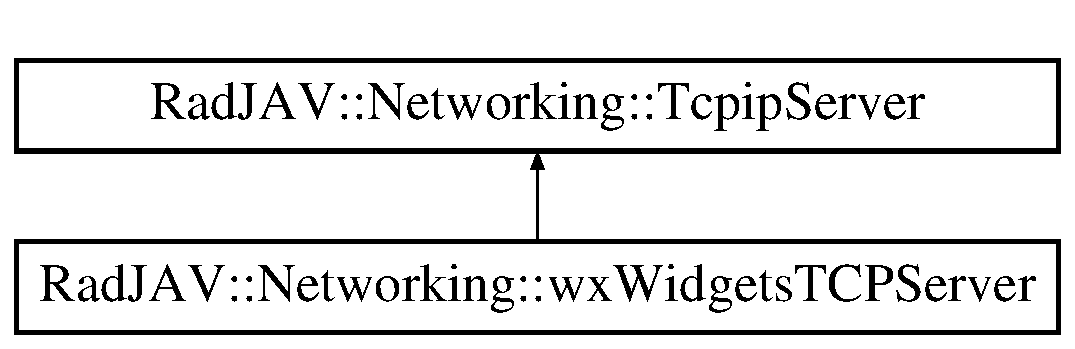
\includegraphics[height=2.000000cm]{class_rad_j_a_v_1_1_networking_1_1wx_widgets_t_c_p_server}
\end{center}
\end{figure}
\subsection*{Public Member Functions}
\begin{DoxyCompactItemize}
\item 
\hyperlink{class_rad_j_a_v_1_1_networking_1_1wx_widgets_t_c_p_server_ac000741f10b0be7e6800f948fba6cdc8}{wx\+Widgets\+T\+C\+P\+Server} ()
\item 
bool \hyperlink{class_rad_j_a_v_1_1_networking_1_1wx_widgets_t_c_p_server_aa0c34e3462f10c401629f9cea3a113a4}{init} (unsigned short new\+Port)
\begin{DoxyCompactList}\small\item\em Start the server. \end{DoxyCompactList}\item 
bool \hyperlink{class_rad_j_a_v_1_1_networking_1_1wx_widgets_t_c_p_server_a09b2a943dc69cab1aa3bf1573a8f72c1}{accept\+With\+Blocking} ()
\item 
bool \hyperlink{class_rad_j_a_v_1_1_networking_1_1wx_widgets_t_c_p_server_a1e78417fa012bebbc21fbcf8557c8008}{accept\+Without\+Blocking} ()
\item 
bool \hyperlink{class_rad_j_a_v_1_1_networking_1_1wx_widgets_t_c_p_server_a42d29962406a990eeeaa97014fae1921}{send\+Float\+To\+All} (float f\+Float, std\+::vector$<$ unsigned int $>$ ary\+Except=std\+::vector$<$ unsigned int $>$())
\item 
bool \hyperlink{class_rad_j_a_v_1_1_networking_1_1wx_widgets_t_c_p_server_a2c0f9bf6466f22c44cba8921b2086d4a}{send\+Float} (wx\+Socket\+Base $\ast$soc\+Socket, float f\+Float)
\item 
bool \hyperlink{class_rad_j_a_v_1_1_networking_1_1wx_widgets_t_c_p_server_a0a575ffac3793d7713d1ba30a64f79e8}{send\+Double\+To\+All} (double d\+Double, std\+::vector$<$ unsigned int $>$ ary\+Except=std\+::vector$<$ unsigned int $>$())
\item 
bool \hyperlink{class_rad_j_a_v_1_1_networking_1_1wx_widgets_t_c_p_server_a9cc3924985547cc4e63be3d91b57e94a}{send\+Double} (wx\+Socket\+Base $\ast$soc\+Socket, double d\+Double)
\item 
bool \hyperlink{class_rad_j_a_v_1_1_networking_1_1wx_widgets_t_c_p_server_a88939471a8291c875699b5c21897be8f}{send\+Int\+To\+All} (int i\+Int, std\+::vector$<$ unsigned int $>$ ary\+Except=std\+::vector$<$ unsigned int $>$())
\item 
bool \hyperlink{class_rad_j_a_v_1_1_networking_1_1wx_widgets_t_c_p_server_a61087019c5c04e8f53f5ab72cacd4535}{send\+Int} (wx\+Socket\+Base $\ast$soc\+Socket, int i\+Int)
\item 
bool \hyperlink{class_rad_j_a_v_1_1_networking_1_1wx_widgets_t_c_p_server_a47832f18cdf7bee7b162c65986042041}{send\+U\+Int\+To\+All} (unsigned int ui\+Int, std\+::vector$<$ unsigned int $>$ ary\+Except=std\+::vector$<$ unsigned int $>$())
\item 
bool \hyperlink{class_rad_j_a_v_1_1_networking_1_1wx_widgets_t_c_p_server_af85993c2e1af60c0867c827c64cb0064}{send\+U\+Int} (wx\+Socket\+Base $\ast$soc\+Socket, unsigned int ui\+Int)
\item 
bool \hyperlink{class_rad_j_a_v_1_1_networking_1_1wx_widgets_t_c_p_server_a6a86177efba9d0d84ed34358b7d417a7}{send\+Long\+To\+All} (long l\+Long, std\+::vector$<$ unsigned int $>$ ary\+Except=std\+::vector$<$ unsigned int $>$())
\item 
bool \hyperlink{class_rad_j_a_v_1_1_networking_1_1wx_widgets_t_c_p_server_a82159c7ca10a3e5267936e8c02c8fbbc}{send\+Long} (wx\+Socket\+Base $\ast$soc\+Socket, long l\+Long)
\item 
bool \hyperlink{class_rad_j_a_v_1_1_networking_1_1wx_widgets_t_c_p_server_afce0d88374bfbd8ed5bc1f0eb67669d3}{send\+U\+Long\+To\+All} (unsigned long ul\+Long, std\+::vector$<$ unsigned int $>$ ary\+Except=std\+::vector$<$ unsigned int $>$())
\item 
bool \hyperlink{class_rad_j_a_v_1_1_networking_1_1wx_widgets_t_c_p_server_a45d4749373218af45168ac52b9cb7881}{send\+U\+Long} (wx\+Socket\+Base $\ast$soc\+Socket, unsigned long ul\+Long)
\item 
bool \hyperlink{class_rad_j_a_v_1_1_networking_1_1wx_widgets_t_c_p_server_a6d6fb3552b75634646d525d2c23e4904}{send\+Short\+To\+All} (short s\+Short, std\+::vector$<$ unsigned int $>$ ary\+Except=std\+::vector$<$ unsigned int $>$())
\item 
bool \hyperlink{class_rad_j_a_v_1_1_networking_1_1wx_widgets_t_c_p_server_a109a7cfe9f0aed3c0ab385e22b7dccfc}{send\+Short} (wx\+Socket\+Base $\ast$soc\+Socket, short s\+Short)
\item 
bool \hyperlink{class_rad_j_a_v_1_1_networking_1_1wx_widgets_t_c_p_server_a5f4d94b2c8d1972c3b01c6de0eee3fc6}{send\+U\+Short\+To\+All} (unsigned short us\+Short, std\+::vector$<$ unsigned int $>$ ary\+Except=std\+::vector$<$ unsigned int $>$())
\item 
bool \hyperlink{class_rad_j_a_v_1_1_networking_1_1wx_widgets_t_c_p_server_ab0c0c636b5b9eedba7402d18f177005d}{send\+U\+Short} (wx\+Socket\+Base $\ast$soc\+Socket, unsigned short us\+Short)
\item 
bool \hyperlink{class_rad_j_a_v_1_1_networking_1_1wx_widgets_t_c_p_server_aa6f6b6b62002a95f65ed1746a25d3048}{send\+Char\+To\+All} (char c\+Char, std\+::vector$<$ unsigned int $>$ ary\+Except=std\+::vector$<$ unsigned int $>$())
\item 
bool \hyperlink{class_rad_j_a_v_1_1_networking_1_1wx_widgets_t_c_p_server_ae40280956d8bba29f636b6104c08b719}{send\+Char} (wx\+Socket\+Base $\ast$soc\+Socket, char c\+Char)
\item 
bool \hyperlink{class_rad_j_a_v_1_1_networking_1_1wx_widgets_t_c_p_server_a74a6dd1c944b3781e2ed286f14d79813}{send\+U\+Char\+To\+All} (unsigned char uc\+Char, std\+::vector$<$ unsigned int $>$ ary\+Except=std\+::vector$<$ unsigned int $>$())
\item 
bool \hyperlink{class_rad_j_a_v_1_1_networking_1_1wx_widgets_t_c_p_server_adf18ccc8867bb45e801a0ad699e14cbe}{send\+U\+Char} (wx\+Socket\+Base $\ast$soc\+Socket, unsigned char uc\+Char)
\item 
bool \hyperlink{class_rad_j_a_v_1_1_networking_1_1wx_widgets_t_c_p_server_ab94fd4375ec2d5a37951b9004bd8cdae}{send\+String\+To\+All} (\hyperlink{class_rad_j_a_v_1_1_string}{String} str\+Line, std\+::vector$<$ unsigned int $>$ ary\+Except=std\+::vector$<$ unsigned int $>$())
\item 
bool \hyperlink{class_rad_j_a_v_1_1_networking_1_1wx_widgets_t_c_p_server_a60916dc2a924530fe488de6d7d38659b}{send\+String} (wx\+Socket\+Base $\ast$soc\+Socket, \hyperlink{class_rad_j_a_v_1_1_string}{String} str\+Line)
\item 
std\+::vector$<$ \hyperlink{class_rad_j_a_v_1_1_networking_1_1_t_c_p_response}{T\+C\+P\+Response}$<$ float $>$ $>$ \hyperlink{class_rad_j_a_v_1_1_networking_1_1wx_widgets_t_c_p_server_a25f1060df172b7ac485c062d5598ee04}{recv\+Float} ()
\begin{DoxyCompactList}\small\item\em Receive an array of floats from the connected clients. \end{DoxyCompactList}\item 
float \hyperlink{class_rad_j_a_v_1_1_networking_1_1wx_widgets_t_c_p_server_a9296263dca17a376711a36753965dd51}{Recv\+Float} (wx\+Socket\+Base $\ast$soc\+Socket)
\item 
std\+::vector$<$ \hyperlink{class_rad_j_a_v_1_1_networking_1_1_t_c_p_response}{T\+C\+P\+Response}$<$ double $>$ $>$ \hyperlink{class_rad_j_a_v_1_1_networking_1_1wx_widgets_t_c_p_server_a1c445d2b459e6a249ec132da08f230bd}{recv\+Double} ()
\begin{DoxyCompactList}\small\item\em Receive an array of doubles from the connected clients. \end{DoxyCompactList}\item 
double \hyperlink{class_rad_j_a_v_1_1_networking_1_1wx_widgets_t_c_p_server_a174193c32b2d90a5b25fd1d44be7e3ac}{Recv\+Double} (wx\+Socket\+Base $\ast$soc\+Socket)
\item 
std\+::vector$<$ \hyperlink{class_rad_j_a_v_1_1_networking_1_1_t_c_p_response}{T\+C\+P\+Response}$<$ int $>$ $>$ \hyperlink{class_rad_j_a_v_1_1_networking_1_1wx_widgets_t_c_p_server_a141060e567ebda7607cf74fe086a8e4c}{recv\+Int} ()
\begin{DoxyCompactList}\small\item\em Receive an array of ints from the connected clients. \end{DoxyCompactList}\item 
int \hyperlink{class_rad_j_a_v_1_1_networking_1_1wx_widgets_t_c_p_server_a6b95b5c066ae471279a2d47cee0a08c9}{Recv\+Int} (wx\+Socket\+Base $\ast$soc\+Socket)
\item 
std\+::vector$<$ \hyperlink{class_rad_j_a_v_1_1_networking_1_1_t_c_p_response}{T\+C\+P\+Response}$<$ unsigned int $>$ $>$ \hyperlink{class_rad_j_a_v_1_1_networking_1_1wx_widgets_t_c_p_server_aefa435e65eef2200e74f1fd903447071}{recv\+U\+Int} ()
\begin{DoxyCompactList}\small\item\em Receive an array of unsigned ints from the connected clients. \end{DoxyCompactList}\item 
unsigned int \hyperlink{class_rad_j_a_v_1_1_networking_1_1wx_widgets_t_c_p_server_abadf9ba29321eee138d88bf2b1390ded}{Recv\+U\+Int} (wx\+Socket\+Base $\ast$soc\+Socket)
\item 
std\+::vector$<$ \hyperlink{class_rad_j_a_v_1_1_networking_1_1_t_c_p_response}{T\+C\+P\+Response}$<$ long $>$ $>$ \hyperlink{class_rad_j_a_v_1_1_networking_1_1wx_widgets_t_c_p_server_aa52be52a0a3aaec2402f838ce39d734d}{recv\+Long} ()
\begin{DoxyCompactList}\small\item\em Receive an array of longs from the connected clients. \end{DoxyCompactList}\item 
long \hyperlink{class_rad_j_a_v_1_1_networking_1_1wx_widgets_t_c_p_server_a1d173552c639864d6e1a27f57b59ff9b}{Recv\+Long} (wx\+Socket\+Base $\ast$soc\+Socket)
\item 
std\+::vector$<$ \hyperlink{class_rad_j_a_v_1_1_networking_1_1_t_c_p_response}{T\+C\+P\+Response}$<$ unsigned long $>$ $>$ \hyperlink{class_rad_j_a_v_1_1_networking_1_1wx_widgets_t_c_p_server_a9330de8d1fe3d184006cbcfb3c88e87f}{recv\+U\+Long} ()
\begin{DoxyCompactList}\small\item\em Receive an array of unsigned longs from the connected clients. \end{DoxyCompactList}\item 
unsigned long \hyperlink{class_rad_j_a_v_1_1_networking_1_1wx_widgets_t_c_p_server_a5ed7e7f894f05987dc9801eed98235e2}{Recv\+U\+Long} (wx\+Socket\+Base $\ast$soc\+Socket)
\item 
std\+::vector$<$ \hyperlink{class_rad_j_a_v_1_1_networking_1_1_t_c_p_response}{T\+C\+P\+Response}$<$ short $>$ $>$ \hyperlink{class_rad_j_a_v_1_1_networking_1_1wx_widgets_t_c_p_server_a28d61fa54cb79db09a4877832e3488ed}{recv\+Short} ()
\begin{DoxyCompactList}\small\item\em Receive an array of shorts from the connected clients. \end{DoxyCompactList}\item 
short \hyperlink{class_rad_j_a_v_1_1_networking_1_1wx_widgets_t_c_p_server_a9ffb0da4edac465b8e4d1ee8c5f3cd18}{Recv\+Short} (wx\+Socket\+Base $\ast$soc\+Socket)
\item 
std\+::vector$<$ \hyperlink{class_rad_j_a_v_1_1_networking_1_1_t_c_p_response}{T\+C\+P\+Response}$<$ unsigned short $>$ $>$ \hyperlink{class_rad_j_a_v_1_1_networking_1_1wx_widgets_t_c_p_server_ad7440dbd5ac95f86a7da35306af67174}{recv\+U\+Short} ()
\begin{DoxyCompactList}\small\item\em Receive an array of unsigned shorts from the connected clients. \end{DoxyCompactList}\item 
unsigned short \hyperlink{class_rad_j_a_v_1_1_networking_1_1wx_widgets_t_c_p_server_a5ffedb767253cf86eff27accd77b5a6f}{Recv\+U\+Short} (wx\+Socket\+Base $\ast$soc\+Socket)
\item 
std\+::vector$<$ \hyperlink{class_rad_j_a_v_1_1_networking_1_1_t_c_p_response}{T\+C\+P\+Response}$<$ char $>$ $>$ \hyperlink{class_rad_j_a_v_1_1_networking_1_1wx_widgets_t_c_p_server_ae964ef6ac1547ac313d8ab580ae3f7b4}{recv\+Char} ()
\begin{DoxyCompactList}\small\item\em Receive an array of chars from the connected clients. \end{DoxyCompactList}\item 
char \hyperlink{class_rad_j_a_v_1_1_networking_1_1wx_widgets_t_c_p_server_a253113c833bf5ac8a384de6d2c61684d}{Recv\+Char} (wx\+Socket\+Base $\ast$soc\+Socket)
\item 
std\+::vector$<$ \hyperlink{class_rad_j_a_v_1_1_networking_1_1_t_c_p_response}{T\+C\+P\+Response}$<$ unsigned char $>$ $>$ \hyperlink{class_rad_j_a_v_1_1_networking_1_1wx_widgets_t_c_p_server_ab4f0c794a4711e14b805f0ffde01160c}{recv\+U\+Char} ()
\begin{DoxyCompactList}\small\item\em Receive an array of unsigned chars from the connected clients. \end{DoxyCompactList}\item 
unsigned char \hyperlink{class_rad_j_a_v_1_1_networking_1_1wx_widgets_t_c_p_server_a424a50ecae9cde2a17b90e6a0fd2f32f}{Recv\+U\+Char} (wx\+Socket\+Base $\ast$soc\+Socket)
\item 
std\+::vector$<$ \hyperlink{class_rad_j_a_v_1_1_networking_1_1_t_c_p_response}{T\+C\+P\+Response}$<$ char $\ast$ $>$ $>$ \hyperlink{class_rad_j_a_v_1_1_networking_1_1wx_widgets_t_c_p_server_a6b3ea7891f3111f89cd1610a9b1db15d}{recv\+String} (int i\+Length)
\begin{DoxyCompactList}\small\item\em Receive a char array from the connected clients. \end{DoxyCompactList}\item 
char $\ast$ \hyperlink{class_rad_j_a_v_1_1_networking_1_1wx_widgets_t_c_p_server_add4a137d2a89f6fb6a64c7b8055f46c2}{Recv\+String} (wx\+Socket\+Base $\ast$soc\+Socket, int i\+Length)
\item 
std\+::vector$<$ \hyperlink{class_rad_j_a_v_1_1_networking_1_1_t_c_p_response}{T\+C\+P\+Response}$<$ \hyperlink{class_rad_j_a_v_1_1_string}{String} $>$ $>$ \hyperlink{class_rad_j_a_v_1_1_networking_1_1wx_widgets_t_c_p_server_ac33b6977b1d527476c8f95eb91464fd9}{recv\+String} ()
\begin{DoxyCompactList}\small\item\em Receive an array of strings from the connected clients. \end{DoxyCompactList}\item 
\hyperlink{class_rad_j_a_v_1_1_string}{String} \hyperlink{class_rad_j_a_v_1_1_networking_1_1wx_widgets_t_c_p_server_ae10f57d8657a085aaad9ea967cfcdda3}{Recv\+String} (wx\+Socket\+Base $\ast$soc\+Socket)
\item 
void \hyperlink{class_rad_j_a_v_1_1_networking_1_1wx_widgets_t_c_p_server_a3779c06a1fca6293155a34008ae044d3}{Set\+Port} (unsigned short us\+Port\+Pass)
\item 
unsigned short \hyperlink{class_rad_j_a_v_1_1_networking_1_1wx_widgets_t_c_p_server_a0a8c3796d3ea9536001e993155f9ffca}{Get\+Port} ()
\item 
void \hyperlink{class_rad_j_a_v_1_1_networking_1_1wx_widgets_t_c_p_server_af1f01bbea328dbb2024f49ea0a078300}{Set\+Server\+Addr} (wx\+I\+P\+V4address adr\+Server\+Pass)
\item 
wx\+I\+P\+V4address \hyperlink{class_rad_j_a_v_1_1_networking_1_1wx_widgets_t_c_p_server_a95f0ce3c74eaa8e5482b7a47c3c4afd4}{Get\+Server\+Addr} ()
\item 
void \hyperlink{class_rad_j_a_v_1_1_networking_1_1wx_widgets_t_c_p_server_a3e088be7abe0d7306546bc76f665a24e}{Set\+Server\+Socket} (wx\+Socket\+Server $\ast$ary\+Sockets\+Pass)
\item 
wx\+Socket\+Server $\ast$ \hyperlink{class_rad_j_a_v_1_1_networking_1_1wx_widgets_t_c_p_server_ad4131a0658edc2d70ee89221e6fa417a}{Get\+Server\+Socket} ()
\item 
void \hyperlink{class_rad_j_a_v_1_1_networking_1_1wx_widgets_t_c_p_server_afdbe6afcd98c24ca8c5284dfd60a7682}{Set\+Client\+Sockets} (std\+::vector$<$ wx\+Socket\+Base $\ast$ $>$ ary\+Sockets\+Pass)
\item 
std\+::vector$<$ wx\+Socket\+Base $\ast$ $>$ \hyperlink{class_rad_j_a_v_1_1_networking_1_1wx_widgets_t_c_p_server_a7bb7ecbbb9b2c6a363bbf972eb3a1626}{Get\+Client\+Sockets} ()
\item 
wx\+Socket\+Base $\ast$ \hyperlink{class_rad_j_a_v_1_1_networking_1_1wx_widgets_t_c_p_server_abccb4388bb5da5f597c9be492f93b45e}{Get\+Client\+Socket} (unsigned int ui\+Id)
\item 
std\+::vector$<$ \hyperlink{class_rad_j_a_v_1_1_string}{String} $>$ \hyperlink{class_rad_j_a_v_1_1_networking_1_1wx_widgets_t_c_p_server_a34eace4489a5e639b9480ea307daf16d}{Get\+Connected\+I\+Ps} ()
\item 
\hyperlink{class_rad_j_a_v_1_1_string}{String} \hyperlink{class_rad_j_a_v_1_1_networking_1_1wx_widgets_t_c_p_server_a5fd51ffee2812c7b94a5ffcd97f24f04}{Get\+Connected\+Ip} (unsigned int ui\+Id)
\item 
\hyperlink{class_rad_j_a_v_1_1_string}{String} \hyperlink{class_rad_j_a_v_1_1_networking_1_1wx_widgets_t_c_p_server_a9b53e846668e7a9c99e95a4d5ea1e6ec}{Get\+Last\+Connected\+Ip} ()
\item 
std\+::vector$<$ unsigned int $>$ \hyperlink{class_rad_j_a_v_1_1_networking_1_1wx_widgets_t_c_p_server_a8c5c5a3f9fcabd44b003259ef55ba599}{Get\+Last\+Received\+From\+List} ()
\item 
\hyperlink{class_rad_j_a_v_1_1_string}{String} \hyperlink{class_rad_j_a_v_1_1_networking_1_1wx_widgets_t_c_p_server_a1d60f5ce0c16c5788fb9b9cb1fe0fa88}{Get\+Last\+Error} ()
\item 
bool \hyperlink{class_rad_j_a_v_1_1_networking_1_1wx_widgets_t_c_p_server_a9d98e3e750d9040db42389f82e0f74f9}{Is\+Socket\+Open} (wx\+Socket\+Base $\ast$soc\+Socket)
\item 
bool \hyperlink{class_rad_j_a_v_1_1_networking_1_1wx_widgets_t_c_p_server_a39bcdb370eee7e96c0bce1429038c548}{Close\+Server\+Socket} ()
\item 
bool \hyperlink{class_rad_j_a_v_1_1_networking_1_1wx_widgets_t_c_p_server_a462129a4742f6b752b2cc57670555606}{Close\+Client\+Socket} (wx\+Socket\+Base $\ast$soc\+Socket)
\item 
bool \hyperlink{class_rad_j_a_v_1_1_networking_1_1wx_widgets_t_c_p_server_a83718025ada3888b0cb3eab89ab9e97f}{Close\+All\+Sockets} ()
\end{DoxyCompactItemize}


\subsection{Constructor \& Destructor Documentation}
\index{Rad\+J\+A\+V\+::\+Networking\+::wx\+Widgets\+T\+C\+P\+Server@{Rad\+J\+A\+V\+::\+Networking\+::wx\+Widgets\+T\+C\+P\+Server}!wx\+Widgets\+T\+C\+P\+Server@{wx\+Widgets\+T\+C\+P\+Server}}
\index{wx\+Widgets\+T\+C\+P\+Server@{wx\+Widgets\+T\+C\+P\+Server}!Rad\+J\+A\+V\+::\+Networking\+::wx\+Widgets\+T\+C\+P\+Server@{Rad\+J\+A\+V\+::\+Networking\+::wx\+Widgets\+T\+C\+P\+Server}}
\subsubsection[{\texorpdfstring{wx\+Widgets\+T\+C\+P\+Server()}{wxWidgetsTCPServer()}}]{\setlength{\rightskip}{0pt plus 5cm}Rad\+J\+A\+V\+::\+Networking\+::wx\+Widgets\+T\+C\+P\+Server\+::wx\+Widgets\+T\+C\+P\+Server (
\begin{DoxyParamCaption}
{}
\end{DoxyParamCaption}
)}\hypertarget{class_rad_j_a_v_1_1_networking_1_1wx_widgets_t_c_p_server_ac000741f10b0be7e6800f948fba6cdc8}{}\label{class_rad_j_a_v_1_1_networking_1_1wx_widgets_t_c_p_server_ac000741f10b0be7e6800f948fba6cdc8}


\subsection{Member Function Documentation}
\index{Rad\+J\+A\+V\+::\+Networking\+::wx\+Widgets\+T\+C\+P\+Server@{Rad\+J\+A\+V\+::\+Networking\+::wx\+Widgets\+T\+C\+P\+Server}!accept\+With\+Blocking@{accept\+With\+Blocking}}
\index{accept\+With\+Blocking@{accept\+With\+Blocking}!Rad\+J\+A\+V\+::\+Networking\+::wx\+Widgets\+T\+C\+P\+Server@{Rad\+J\+A\+V\+::\+Networking\+::wx\+Widgets\+T\+C\+P\+Server}}
\subsubsection[{\texorpdfstring{accept\+With\+Blocking()}{acceptWithBlocking()}}]{\setlength{\rightskip}{0pt plus 5cm}bool Rad\+J\+A\+V\+::\+Networking\+::wx\+Widgets\+T\+C\+P\+Server\+::accept\+With\+Blocking (
\begin{DoxyParamCaption}
{}
\end{DoxyParamCaption}
)\hspace{0.3cm}{\ttfamily [virtual]}}\hypertarget{class_rad_j_a_v_1_1_networking_1_1wx_widgets_t_c_p_server_a09b2a943dc69cab1aa3bf1573a8f72c1}{}\label{class_rad_j_a_v_1_1_networking_1_1wx_widgets_t_c_p_server_a09b2a943dc69cab1aa3bf1573a8f72c1}
Listen for connections and lock the current thread. 

Implements \hyperlink{class_rad_j_a_v_1_1_networking_1_1_tcpip_server_a53555ae267a5f3d6ac8aafbb7a567ee9}{Rad\+J\+A\+V\+::\+Networking\+::\+Tcpip\+Server}.

\index{Rad\+J\+A\+V\+::\+Networking\+::wx\+Widgets\+T\+C\+P\+Server@{Rad\+J\+A\+V\+::\+Networking\+::wx\+Widgets\+T\+C\+P\+Server}!accept\+Without\+Blocking@{accept\+Without\+Blocking}}
\index{accept\+Without\+Blocking@{accept\+Without\+Blocking}!Rad\+J\+A\+V\+::\+Networking\+::wx\+Widgets\+T\+C\+P\+Server@{Rad\+J\+A\+V\+::\+Networking\+::wx\+Widgets\+T\+C\+P\+Server}}
\subsubsection[{\texorpdfstring{accept\+Without\+Blocking()}{acceptWithoutBlocking()}}]{\setlength{\rightskip}{0pt plus 5cm}bool Rad\+J\+A\+V\+::\+Networking\+::wx\+Widgets\+T\+C\+P\+Server\+::accept\+Without\+Blocking (
\begin{DoxyParamCaption}
{}
\end{DoxyParamCaption}
)\hspace{0.3cm}{\ttfamily [virtual]}}\hypertarget{class_rad_j_a_v_1_1_networking_1_1wx_widgets_t_c_p_server_a1e78417fa012bebbc21fbcf8557c8008}{}\label{class_rad_j_a_v_1_1_networking_1_1wx_widgets_t_c_p_server_a1e78417fa012bebbc21fbcf8557c8008}
Listen for connections and do not lock the current thread. 

Implements \hyperlink{class_rad_j_a_v_1_1_networking_1_1_tcpip_server_a3d7ea19180509cffa6d4ee802767ca90}{Rad\+J\+A\+V\+::\+Networking\+::\+Tcpip\+Server}.

\index{Rad\+J\+A\+V\+::\+Networking\+::wx\+Widgets\+T\+C\+P\+Server@{Rad\+J\+A\+V\+::\+Networking\+::wx\+Widgets\+T\+C\+P\+Server}!Close\+All\+Sockets@{Close\+All\+Sockets}}
\index{Close\+All\+Sockets@{Close\+All\+Sockets}!Rad\+J\+A\+V\+::\+Networking\+::wx\+Widgets\+T\+C\+P\+Server@{Rad\+J\+A\+V\+::\+Networking\+::wx\+Widgets\+T\+C\+P\+Server}}
\subsubsection[{\texorpdfstring{Close\+All\+Sockets()}{CloseAllSockets()}}]{\setlength{\rightskip}{0pt plus 5cm}bool Rad\+J\+A\+V\+::\+Networking\+::wx\+Widgets\+T\+C\+P\+Server\+::\+Close\+All\+Sockets (
\begin{DoxyParamCaption}
{}
\end{DoxyParamCaption}
)}\hypertarget{class_rad_j_a_v_1_1_networking_1_1wx_widgets_t_c_p_server_a83718025ada3888b0cb3eab89ab9e97f}{}\label{class_rad_j_a_v_1_1_networking_1_1wx_widgets_t_c_p_server_a83718025ada3888b0cb3eab89ab9e97f}
\index{Rad\+J\+A\+V\+::\+Networking\+::wx\+Widgets\+T\+C\+P\+Server@{Rad\+J\+A\+V\+::\+Networking\+::wx\+Widgets\+T\+C\+P\+Server}!Close\+Client\+Socket@{Close\+Client\+Socket}}
\index{Close\+Client\+Socket@{Close\+Client\+Socket}!Rad\+J\+A\+V\+::\+Networking\+::wx\+Widgets\+T\+C\+P\+Server@{Rad\+J\+A\+V\+::\+Networking\+::wx\+Widgets\+T\+C\+P\+Server}}
\subsubsection[{\texorpdfstring{Close\+Client\+Socket(wx\+Socket\+Base $\ast$soc\+Socket)}{CloseClientSocket(wxSocketBase *socSocket)}}]{\setlength{\rightskip}{0pt plus 5cm}bool Rad\+J\+A\+V\+::\+Networking\+::wx\+Widgets\+T\+C\+P\+Server\+::\+Close\+Client\+Socket (
\begin{DoxyParamCaption}
\item[{wx\+Socket\+Base $\ast$}]{soc\+Socket}
\end{DoxyParamCaption}
)}\hypertarget{class_rad_j_a_v_1_1_networking_1_1wx_widgets_t_c_p_server_a462129a4742f6b752b2cc57670555606}{}\label{class_rad_j_a_v_1_1_networking_1_1wx_widgets_t_c_p_server_a462129a4742f6b752b2cc57670555606}
\index{Rad\+J\+A\+V\+::\+Networking\+::wx\+Widgets\+T\+C\+P\+Server@{Rad\+J\+A\+V\+::\+Networking\+::wx\+Widgets\+T\+C\+P\+Server}!Close\+Server\+Socket@{Close\+Server\+Socket}}
\index{Close\+Server\+Socket@{Close\+Server\+Socket}!Rad\+J\+A\+V\+::\+Networking\+::wx\+Widgets\+T\+C\+P\+Server@{Rad\+J\+A\+V\+::\+Networking\+::wx\+Widgets\+T\+C\+P\+Server}}
\subsubsection[{\texorpdfstring{Close\+Server\+Socket()}{CloseServerSocket()}}]{\setlength{\rightskip}{0pt plus 5cm}bool Rad\+J\+A\+V\+::\+Networking\+::wx\+Widgets\+T\+C\+P\+Server\+::\+Close\+Server\+Socket (
\begin{DoxyParamCaption}
{}
\end{DoxyParamCaption}
)}\hypertarget{class_rad_j_a_v_1_1_networking_1_1wx_widgets_t_c_p_server_a39bcdb370eee7e96c0bce1429038c548}{}\label{class_rad_j_a_v_1_1_networking_1_1wx_widgets_t_c_p_server_a39bcdb370eee7e96c0bce1429038c548}
\index{Rad\+J\+A\+V\+::\+Networking\+::wx\+Widgets\+T\+C\+P\+Server@{Rad\+J\+A\+V\+::\+Networking\+::wx\+Widgets\+T\+C\+P\+Server}!Get\+Client\+Socket@{Get\+Client\+Socket}}
\index{Get\+Client\+Socket@{Get\+Client\+Socket}!Rad\+J\+A\+V\+::\+Networking\+::wx\+Widgets\+T\+C\+P\+Server@{Rad\+J\+A\+V\+::\+Networking\+::wx\+Widgets\+T\+C\+P\+Server}}
\subsubsection[{\texorpdfstring{Get\+Client\+Socket(unsigned int ui\+Id)}{GetClientSocket(unsigned int uiId)}}]{\setlength{\rightskip}{0pt plus 5cm}wx\+Socket\+Base $\ast$ Rad\+J\+A\+V\+::\+Networking\+::wx\+Widgets\+T\+C\+P\+Server\+::\+Get\+Client\+Socket (
\begin{DoxyParamCaption}
\item[{unsigned int}]{ui\+Id}
\end{DoxyParamCaption}
)}\hypertarget{class_rad_j_a_v_1_1_networking_1_1wx_widgets_t_c_p_server_abccb4388bb5da5f597c9be492f93b45e}{}\label{class_rad_j_a_v_1_1_networking_1_1wx_widgets_t_c_p_server_abccb4388bb5da5f597c9be492f93b45e}
\index{Rad\+J\+A\+V\+::\+Networking\+::wx\+Widgets\+T\+C\+P\+Server@{Rad\+J\+A\+V\+::\+Networking\+::wx\+Widgets\+T\+C\+P\+Server}!Get\+Client\+Sockets@{Get\+Client\+Sockets}}
\index{Get\+Client\+Sockets@{Get\+Client\+Sockets}!Rad\+J\+A\+V\+::\+Networking\+::wx\+Widgets\+T\+C\+P\+Server@{Rad\+J\+A\+V\+::\+Networking\+::wx\+Widgets\+T\+C\+P\+Server}}
\subsubsection[{\texorpdfstring{Get\+Client\+Sockets()}{GetClientSockets()}}]{\setlength{\rightskip}{0pt plus 5cm}std\+::vector$<$ wx\+Socket\+Base $\ast$ $>$ Rad\+J\+A\+V\+::\+Networking\+::wx\+Widgets\+T\+C\+P\+Server\+::\+Get\+Client\+Sockets (
\begin{DoxyParamCaption}
{}
\end{DoxyParamCaption}
)}\hypertarget{class_rad_j_a_v_1_1_networking_1_1wx_widgets_t_c_p_server_a7bb7ecbbb9b2c6a363bbf972eb3a1626}{}\label{class_rad_j_a_v_1_1_networking_1_1wx_widgets_t_c_p_server_a7bb7ecbbb9b2c6a363bbf972eb3a1626}
\index{Rad\+J\+A\+V\+::\+Networking\+::wx\+Widgets\+T\+C\+P\+Server@{Rad\+J\+A\+V\+::\+Networking\+::wx\+Widgets\+T\+C\+P\+Server}!Get\+Connected\+Ip@{Get\+Connected\+Ip}}
\index{Get\+Connected\+Ip@{Get\+Connected\+Ip}!Rad\+J\+A\+V\+::\+Networking\+::wx\+Widgets\+T\+C\+P\+Server@{Rad\+J\+A\+V\+::\+Networking\+::wx\+Widgets\+T\+C\+P\+Server}}
\subsubsection[{\texorpdfstring{Get\+Connected\+Ip(unsigned int ui\+Id)}{GetConnectedIp(unsigned int uiId)}}]{\setlength{\rightskip}{0pt plus 5cm}{\bf String} Rad\+J\+A\+V\+::\+Networking\+::wx\+Widgets\+T\+C\+P\+Server\+::\+Get\+Connected\+Ip (
\begin{DoxyParamCaption}
\item[{unsigned int}]{ui\+Id}
\end{DoxyParamCaption}
)}\hypertarget{class_rad_j_a_v_1_1_networking_1_1wx_widgets_t_c_p_server_a5fd51ffee2812c7b94a5ffcd97f24f04}{}\label{class_rad_j_a_v_1_1_networking_1_1wx_widgets_t_c_p_server_a5fd51ffee2812c7b94a5ffcd97f24f04}
\index{Rad\+J\+A\+V\+::\+Networking\+::wx\+Widgets\+T\+C\+P\+Server@{Rad\+J\+A\+V\+::\+Networking\+::wx\+Widgets\+T\+C\+P\+Server}!Get\+Connected\+I\+Ps@{Get\+Connected\+I\+Ps}}
\index{Get\+Connected\+I\+Ps@{Get\+Connected\+I\+Ps}!Rad\+J\+A\+V\+::\+Networking\+::wx\+Widgets\+T\+C\+P\+Server@{Rad\+J\+A\+V\+::\+Networking\+::wx\+Widgets\+T\+C\+P\+Server}}
\subsubsection[{\texorpdfstring{Get\+Connected\+I\+Ps()}{GetConnectedIPs()}}]{\setlength{\rightskip}{0pt plus 5cm}std\+::vector$<$ {\bf String} $>$ Rad\+J\+A\+V\+::\+Networking\+::wx\+Widgets\+T\+C\+P\+Server\+::\+Get\+Connected\+I\+Ps (
\begin{DoxyParamCaption}
{}
\end{DoxyParamCaption}
)}\hypertarget{class_rad_j_a_v_1_1_networking_1_1wx_widgets_t_c_p_server_a34eace4489a5e639b9480ea307daf16d}{}\label{class_rad_j_a_v_1_1_networking_1_1wx_widgets_t_c_p_server_a34eace4489a5e639b9480ea307daf16d}
\index{Rad\+J\+A\+V\+::\+Networking\+::wx\+Widgets\+T\+C\+P\+Server@{Rad\+J\+A\+V\+::\+Networking\+::wx\+Widgets\+T\+C\+P\+Server}!Get\+Last\+Connected\+Ip@{Get\+Last\+Connected\+Ip}}
\index{Get\+Last\+Connected\+Ip@{Get\+Last\+Connected\+Ip}!Rad\+J\+A\+V\+::\+Networking\+::wx\+Widgets\+T\+C\+P\+Server@{Rad\+J\+A\+V\+::\+Networking\+::wx\+Widgets\+T\+C\+P\+Server}}
\subsubsection[{\texorpdfstring{Get\+Last\+Connected\+Ip()}{GetLastConnectedIp()}}]{\setlength{\rightskip}{0pt plus 5cm}{\bf String} Rad\+J\+A\+V\+::\+Networking\+::wx\+Widgets\+T\+C\+P\+Server\+::\+Get\+Last\+Connected\+Ip (
\begin{DoxyParamCaption}
{}
\end{DoxyParamCaption}
)}\hypertarget{class_rad_j_a_v_1_1_networking_1_1wx_widgets_t_c_p_server_a9b53e846668e7a9c99e95a4d5ea1e6ec}{}\label{class_rad_j_a_v_1_1_networking_1_1wx_widgets_t_c_p_server_a9b53e846668e7a9c99e95a4d5ea1e6ec}
\index{Rad\+J\+A\+V\+::\+Networking\+::wx\+Widgets\+T\+C\+P\+Server@{Rad\+J\+A\+V\+::\+Networking\+::wx\+Widgets\+T\+C\+P\+Server}!Get\+Last\+Error@{Get\+Last\+Error}}
\index{Get\+Last\+Error@{Get\+Last\+Error}!Rad\+J\+A\+V\+::\+Networking\+::wx\+Widgets\+T\+C\+P\+Server@{Rad\+J\+A\+V\+::\+Networking\+::wx\+Widgets\+T\+C\+P\+Server}}
\subsubsection[{\texorpdfstring{Get\+Last\+Error()}{GetLastError()}}]{\setlength{\rightskip}{0pt plus 5cm}{\bf String} Rad\+J\+A\+V\+::\+Networking\+::wx\+Widgets\+T\+C\+P\+Server\+::\+Get\+Last\+Error (
\begin{DoxyParamCaption}
{}
\end{DoxyParamCaption}
)}\hypertarget{class_rad_j_a_v_1_1_networking_1_1wx_widgets_t_c_p_server_a1d60f5ce0c16c5788fb9b9cb1fe0fa88}{}\label{class_rad_j_a_v_1_1_networking_1_1wx_widgets_t_c_p_server_a1d60f5ce0c16c5788fb9b9cb1fe0fa88}
\index{Rad\+J\+A\+V\+::\+Networking\+::wx\+Widgets\+T\+C\+P\+Server@{Rad\+J\+A\+V\+::\+Networking\+::wx\+Widgets\+T\+C\+P\+Server}!Get\+Last\+Received\+From\+List@{Get\+Last\+Received\+From\+List}}
\index{Get\+Last\+Received\+From\+List@{Get\+Last\+Received\+From\+List}!Rad\+J\+A\+V\+::\+Networking\+::wx\+Widgets\+T\+C\+P\+Server@{Rad\+J\+A\+V\+::\+Networking\+::wx\+Widgets\+T\+C\+P\+Server}}
\subsubsection[{\texorpdfstring{Get\+Last\+Received\+From\+List()}{GetLastReceivedFromList()}}]{\setlength{\rightskip}{0pt plus 5cm}std\+::vector$<$ unsigned int $>$ Rad\+J\+A\+V\+::\+Networking\+::wx\+Widgets\+T\+C\+P\+Server\+::\+Get\+Last\+Received\+From\+List (
\begin{DoxyParamCaption}
{}
\end{DoxyParamCaption}
)}\hypertarget{class_rad_j_a_v_1_1_networking_1_1wx_widgets_t_c_p_server_a8c5c5a3f9fcabd44b003259ef55ba599}{}\label{class_rad_j_a_v_1_1_networking_1_1wx_widgets_t_c_p_server_a8c5c5a3f9fcabd44b003259ef55ba599}
\index{Rad\+J\+A\+V\+::\+Networking\+::wx\+Widgets\+T\+C\+P\+Server@{Rad\+J\+A\+V\+::\+Networking\+::wx\+Widgets\+T\+C\+P\+Server}!Get\+Port@{Get\+Port}}
\index{Get\+Port@{Get\+Port}!Rad\+J\+A\+V\+::\+Networking\+::wx\+Widgets\+T\+C\+P\+Server@{Rad\+J\+A\+V\+::\+Networking\+::wx\+Widgets\+T\+C\+P\+Server}}
\subsubsection[{\texorpdfstring{Get\+Port()}{GetPort()}}]{\setlength{\rightskip}{0pt plus 5cm}unsigned short Rad\+J\+A\+V\+::\+Networking\+::wx\+Widgets\+T\+C\+P\+Server\+::\+Get\+Port (
\begin{DoxyParamCaption}
{}
\end{DoxyParamCaption}
)}\hypertarget{class_rad_j_a_v_1_1_networking_1_1wx_widgets_t_c_p_server_a0a8c3796d3ea9536001e993155f9ffca}{}\label{class_rad_j_a_v_1_1_networking_1_1wx_widgets_t_c_p_server_a0a8c3796d3ea9536001e993155f9ffca}
\index{Rad\+J\+A\+V\+::\+Networking\+::wx\+Widgets\+T\+C\+P\+Server@{Rad\+J\+A\+V\+::\+Networking\+::wx\+Widgets\+T\+C\+P\+Server}!Get\+Server\+Addr@{Get\+Server\+Addr}}
\index{Get\+Server\+Addr@{Get\+Server\+Addr}!Rad\+J\+A\+V\+::\+Networking\+::wx\+Widgets\+T\+C\+P\+Server@{Rad\+J\+A\+V\+::\+Networking\+::wx\+Widgets\+T\+C\+P\+Server}}
\subsubsection[{\texorpdfstring{Get\+Server\+Addr()}{GetServerAddr()}}]{\setlength{\rightskip}{0pt plus 5cm}wx\+I\+P\+V4address Rad\+J\+A\+V\+::\+Networking\+::wx\+Widgets\+T\+C\+P\+Server\+::\+Get\+Server\+Addr (
\begin{DoxyParamCaption}
{}
\end{DoxyParamCaption}
)}\hypertarget{class_rad_j_a_v_1_1_networking_1_1wx_widgets_t_c_p_server_a95f0ce3c74eaa8e5482b7a47c3c4afd4}{}\label{class_rad_j_a_v_1_1_networking_1_1wx_widgets_t_c_p_server_a95f0ce3c74eaa8e5482b7a47c3c4afd4}
\index{Rad\+J\+A\+V\+::\+Networking\+::wx\+Widgets\+T\+C\+P\+Server@{Rad\+J\+A\+V\+::\+Networking\+::wx\+Widgets\+T\+C\+P\+Server}!Get\+Server\+Socket@{Get\+Server\+Socket}}
\index{Get\+Server\+Socket@{Get\+Server\+Socket}!Rad\+J\+A\+V\+::\+Networking\+::wx\+Widgets\+T\+C\+P\+Server@{Rad\+J\+A\+V\+::\+Networking\+::wx\+Widgets\+T\+C\+P\+Server}}
\subsubsection[{\texorpdfstring{Get\+Server\+Socket()}{GetServerSocket()}}]{\setlength{\rightskip}{0pt plus 5cm}wx\+Socket\+Server $\ast$ Rad\+J\+A\+V\+::\+Networking\+::wx\+Widgets\+T\+C\+P\+Server\+::\+Get\+Server\+Socket (
\begin{DoxyParamCaption}
{}
\end{DoxyParamCaption}
)}\hypertarget{class_rad_j_a_v_1_1_networking_1_1wx_widgets_t_c_p_server_ad4131a0658edc2d70ee89221e6fa417a}{}\label{class_rad_j_a_v_1_1_networking_1_1wx_widgets_t_c_p_server_ad4131a0658edc2d70ee89221e6fa417a}
\index{Rad\+J\+A\+V\+::\+Networking\+::wx\+Widgets\+T\+C\+P\+Server@{Rad\+J\+A\+V\+::\+Networking\+::wx\+Widgets\+T\+C\+P\+Server}!init@{init}}
\index{init@{init}!Rad\+J\+A\+V\+::\+Networking\+::wx\+Widgets\+T\+C\+P\+Server@{Rad\+J\+A\+V\+::\+Networking\+::wx\+Widgets\+T\+C\+P\+Server}}
\subsubsection[{\texorpdfstring{init(unsigned short new\+Port)}{init(unsigned short newPort)}}]{\setlength{\rightskip}{0pt plus 5cm}bool Rad\+J\+A\+V\+::\+Networking\+::wx\+Widgets\+T\+C\+P\+Server\+::init (
\begin{DoxyParamCaption}
\item[{unsigned short}]{new\+Port}
\end{DoxyParamCaption}
)\hspace{0.3cm}{\ttfamily [virtual]}}\hypertarget{class_rad_j_a_v_1_1_networking_1_1wx_widgets_t_c_p_server_aa0c34e3462f10c401629f9cea3a113a4}{}\label{class_rad_j_a_v_1_1_networking_1_1wx_widgets_t_c_p_server_aa0c34e3462f10c401629f9cea3a113a4}


Start the server. 



Implements \hyperlink{class_rad_j_a_v_1_1_networking_1_1_tcpip_server_a3d67bcb55aae5c4cc937113c2def86b9}{Rad\+J\+A\+V\+::\+Networking\+::\+Tcpip\+Server}.

\index{Rad\+J\+A\+V\+::\+Networking\+::wx\+Widgets\+T\+C\+P\+Server@{Rad\+J\+A\+V\+::\+Networking\+::wx\+Widgets\+T\+C\+P\+Server}!Is\+Socket\+Open@{Is\+Socket\+Open}}
\index{Is\+Socket\+Open@{Is\+Socket\+Open}!Rad\+J\+A\+V\+::\+Networking\+::wx\+Widgets\+T\+C\+P\+Server@{Rad\+J\+A\+V\+::\+Networking\+::wx\+Widgets\+T\+C\+P\+Server}}
\subsubsection[{\texorpdfstring{Is\+Socket\+Open(wx\+Socket\+Base $\ast$soc\+Socket)}{IsSocketOpen(wxSocketBase *socSocket)}}]{\setlength{\rightskip}{0pt plus 5cm}bool Rad\+J\+A\+V\+::\+Networking\+::wx\+Widgets\+T\+C\+P\+Server\+::\+Is\+Socket\+Open (
\begin{DoxyParamCaption}
\item[{wx\+Socket\+Base $\ast$}]{soc\+Socket}
\end{DoxyParamCaption}
)}\hypertarget{class_rad_j_a_v_1_1_networking_1_1wx_widgets_t_c_p_server_a9d98e3e750d9040db42389f82e0f74f9}{}\label{class_rad_j_a_v_1_1_networking_1_1wx_widgets_t_c_p_server_a9d98e3e750d9040db42389f82e0f74f9}
\index{Rad\+J\+A\+V\+::\+Networking\+::wx\+Widgets\+T\+C\+P\+Server@{Rad\+J\+A\+V\+::\+Networking\+::wx\+Widgets\+T\+C\+P\+Server}!recv\+Char@{recv\+Char}}
\index{recv\+Char@{recv\+Char}!Rad\+J\+A\+V\+::\+Networking\+::wx\+Widgets\+T\+C\+P\+Server@{Rad\+J\+A\+V\+::\+Networking\+::wx\+Widgets\+T\+C\+P\+Server}}
\subsubsection[{\texorpdfstring{recv\+Char()}{recvChar()}}]{\setlength{\rightskip}{0pt plus 5cm}std\+::vector$<$ {\bf T\+C\+P\+Response}$<$char$>$ $>$ Rad\+J\+A\+V\+::\+Networking\+::wx\+Widgets\+T\+C\+P\+Server\+::recv\+Char (
\begin{DoxyParamCaption}
{}
\end{DoxyParamCaption}
)\hspace{0.3cm}{\ttfamily [virtual]}}\hypertarget{class_rad_j_a_v_1_1_networking_1_1wx_widgets_t_c_p_server_ae964ef6ac1547ac313d8ab580ae3f7b4}{}\label{class_rad_j_a_v_1_1_networking_1_1wx_widgets_t_c_p_server_ae964ef6ac1547ac313d8ab580ae3f7b4}


Receive an array of chars from the connected clients. 



Implements \hyperlink{class_rad_j_a_v_1_1_networking_1_1_tcpip_server_a1e9b75bd3eccf46033d3c3b0a14c4ced}{Rad\+J\+A\+V\+::\+Networking\+::\+Tcpip\+Server}.

\index{Rad\+J\+A\+V\+::\+Networking\+::wx\+Widgets\+T\+C\+P\+Server@{Rad\+J\+A\+V\+::\+Networking\+::wx\+Widgets\+T\+C\+P\+Server}!Recv\+Char@{Recv\+Char}}
\index{Recv\+Char@{Recv\+Char}!Rad\+J\+A\+V\+::\+Networking\+::wx\+Widgets\+T\+C\+P\+Server@{Rad\+J\+A\+V\+::\+Networking\+::wx\+Widgets\+T\+C\+P\+Server}}
\subsubsection[{\texorpdfstring{Recv\+Char(wx\+Socket\+Base $\ast$soc\+Socket)}{RecvChar(wxSocketBase *socSocket)}}]{\setlength{\rightskip}{0pt plus 5cm}char Rad\+J\+A\+V\+::\+Networking\+::wx\+Widgets\+T\+C\+P\+Server\+::\+Recv\+Char (
\begin{DoxyParamCaption}
\item[{wx\+Socket\+Base $\ast$}]{soc\+Socket}
\end{DoxyParamCaption}
)}\hypertarget{class_rad_j_a_v_1_1_networking_1_1wx_widgets_t_c_p_server_a253113c833bf5ac8a384de6d2c61684d}{}\label{class_rad_j_a_v_1_1_networking_1_1wx_widgets_t_c_p_server_a253113c833bf5ac8a384de6d2c61684d}
\index{Rad\+J\+A\+V\+::\+Networking\+::wx\+Widgets\+T\+C\+P\+Server@{Rad\+J\+A\+V\+::\+Networking\+::wx\+Widgets\+T\+C\+P\+Server}!recv\+Double@{recv\+Double}}
\index{recv\+Double@{recv\+Double}!Rad\+J\+A\+V\+::\+Networking\+::wx\+Widgets\+T\+C\+P\+Server@{Rad\+J\+A\+V\+::\+Networking\+::wx\+Widgets\+T\+C\+P\+Server}}
\subsubsection[{\texorpdfstring{recv\+Double()}{recvDouble()}}]{\setlength{\rightskip}{0pt plus 5cm}std\+::vector$<$ {\bf T\+C\+P\+Response}$<$double$>$ $>$ Rad\+J\+A\+V\+::\+Networking\+::wx\+Widgets\+T\+C\+P\+Server\+::recv\+Double (
\begin{DoxyParamCaption}
{}
\end{DoxyParamCaption}
)\hspace{0.3cm}{\ttfamily [virtual]}}\hypertarget{class_rad_j_a_v_1_1_networking_1_1wx_widgets_t_c_p_server_a1c445d2b459e6a249ec132da08f230bd}{}\label{class_rad_j_a_v_1_1_networking_1_1wx_widgets_t_c_p_server_a1c445d2b459e6a249ec132da08f230bd}


Receive an array of doubles from the connected clients. 



Implements \hyperlink{class_rad_j_a_v_1_1_networking_1_1_tcpip_server_a42628f9e5e784604d970fea3fce7d5c9}{Rad\+J\+A\+V\+::\+Networking\+::\+Tcpip\+Server}.

\index{Rad\+J\+A\+V\+::\+Networking\+::wx\+Widgets\+T\+C\+P\+Server@{Rad\+J\+A\+V\+::\+Networking\+::wx\+Widgets\+T\+C\+P\+Server}!Recv\+Double@{Recv\+Double}}
\index{Recv\+Double@{Recv\+Double}!Rad\+J\+A\+V\+::\+Networking\+::wx\+Widgets\+T\+C\+P\+Server@{Rad\+J\+A\+V\+::\+Networking\+::wx\+Widgets\+T\+C\+P\+Server}}
\subsubsection[{\texorpdfstring{Recv\+Double(wx\+Socket\+Base $\ast$soc\+Socket)}{RecvDouble(wxSocketBase *socSocket)}}]{\setlength{\rightskip}{0pt plus 5cm}double Rad\+J\+A\+V\+::\+Networking\+::wx\+Widgets\+T\+C\+P\+Server\+::\+Recv\+Double (
\begin{DoxyParamCaption}
\item[{wx\+Socket\+Base $\ast$}]{soc\+Socket}
\end{DoxyParamCaption}
)}\hypertarget{class_rad_j_a_v_1_1_networking_1_1wx_widgets_t_c_p_server_a174193c32b2d90a5b25fd1d44be7e3ac}{}\label{class_rad_j_a_v_1_1_networking_1_1wx_widgets_t_c_p_server_a174193c32b2d90a5b25fd1d44be7e3ac}
\index{Rad\+J\+A\+V\+::\+Networking\+::wx\+Widgets\+T\+C\+P\+Server@{Rad\+J\+A\+V\+::\+Networking\+::wx\+Widgets\+T\+C\+P\+Server}!recv\+Float@{recv\+Float}}
\index{recv\+Float@{recv\+Float}!Rad\+J\+A\+V\+::\+Networking\+::wx\+Widgets\+T\+C\+P\+Server@{Rad\+J\+A\+V\+::\+Networking\+::wx\+Widgets\+T\+C\+P\+Server}}
\subsubsection[{\texorpdfstring{recv\+Float()}{recvFloat()}}]{\setlength{\rightskip}{0pt plus 5cm}std\+::vector$<$ {\bf T\+C\+P\+Response}$<$float$>$ $>$ Rad\+J\+A\+V\+::\+Networking\+::wx\+Widgets\+T\+C\+P\+Server\+::recv\+Float (
\begin{DoxyParamCaption}
{}
\end{DoxyParamCaption}
)\hspace{0.3cm}{\ttfamily [virtual]}}\hypertarget{class_rad_j_a_v_1_1_networking_1_1wx_widgets_t_c_p_server_a25f1060df172b7ac485c062d5598ee04}{}\label{class_rad_j_a_v_1_1_networking_1_1wx_widgets_t_c_p_server_a25f1060df172b7ac485c062d5598ee04}


Receive an array of floats from the connected clients. 



Implements \hyperlink{class_rad_j_a_v_1_1_networking_1_1_tcpip_server_a99113c9c8db6b16c804c8efefd0fedae}{Rad\+J\+A\+V\+::\+Networking\+::\+Tcpip\+Server}.

\index{Rad\+J\+A\+V\+::\+Networking\+::wx\+Widgets\+T\+C\+P\+Server@{Rad\+J\+A\+V\+::\+Networking\+::wx\+Widgets\+T\+C\+P\+Server}!Recv\+Float@{Recv\+Float}}
\index{Recv\+Float@{Recv\+Float}!Rad\+J\+A\+V\+::\+Networking\+::wx\+Widgets\+T\+C\+P\+Server@{Rad\+J\+A\+V\+::\+Networking\+::wx\+Widgets\+T\+C\+P\+Server}}
\subsubsection[{\texorpdfstring{Recv\+Float(wx\+Socket\+Base $\ast$soc\+Socket)}{RecvFloat(wxSocketBase *socSocket)}}]{\setlength{\rightskip}{0pt plus 5cm}float Rad\+J\+A\+V\+::\+Networking\+::wx\+Widgets\+T\+C\+P\+Server\+::\+Recv\+Float (
\begin{DoxyParamCaption}
\item[{wx\+Socket\+Base $\ast$}]{soc\+Socket}
\end{DoxyParamCaption}
)}\hypertarget{class_rad_j_a_v_1_1_networking_1_1wx_widgets_t_c_p_server_a9296263dca17a376711a36753965dd51}{}\label{class_rad_j_a_v_1_1_networking_1_1wx_widgets_t_c_p_server_a9296263dca17a376711a36753965dd51}
\index{Rad\+J\+A\+V\+::\+Networking\+::wx\+Widgets\+T\+C\+P\+Server@{Rad\+J\+A\+V\+::\+Networking\+::wx\+Widgets\+T\+C\+P\+Server}!recv\+Int@{recv\+Int}}
\index{recv\+Int@{recv\+Int}!Rad\+J\+A\+V\+::\+Networking\+::wx\+Widgets\+T\+C\+P\+Server@{Rad\+J\+A\+V\+::\+Networking\+::wx\+Widgets\+T\+C\+P\+Server}}
\subsubsection[{\texorpdfstring{recv\+Int()}{recvInt()}}]{\setlength{\rightskip}{0pt plus 5cm}std\+::vector$<$ {\bf T\+C\+P\+Response}$<$int$>$ $>$ Rad\+J\+A\+V\+::\+Networking\+::wx\+Widgets\+T\+C\+P\+Server\+::recv\+Int (
\begin{DoxyParamCaption}
{}
\end{DoxyParamCaption}
)\hspace{0.3cm}{\ttfamily [virtual]}}\hypertarget{class_rad_j_a_v_1_1_networking_1_1wx_widgets_t_c_p_server_a141060e567ebda7607cf74fe086a8e4c}{}\label{class_rad_j_a_v_1_1_networking_1_1wx_widgets_t_c_p_server_a141060e567ebda7607cf74fe086a8e4c}


Receive an array of ints from the connected clients. 



Implements \hyperlink{class_rad_j_a_v_1_1_networking_1_1_tcpip_server_a728b63e038645a7da857c1e1e628a249}{Rad\+J\+A\+V\+::\+Networking\+::\+Tcpip\+Server}.

\index{Rad\+J\+A\+V\+::\+Networking\+::wx\+Widgets\+T\+C\+P\+Server@{Rad\+J\+A\+V\+::\+Networking\+::wx\+Widgets\+T\+C\+P\+Server}!Recv\+Int@{Recv\+Int}}
\index{Recv\+Int@{Recv\+Int}!Rad\+J\+A\+V\+::\+Networking\+::wx\+Widgets\+T\+C\+P\+Server@{Rad\+J\+A\+V\+::\+Networking\+::wx\+Widgets\+T\+C\+P\+Server}}
\subsubsection[{\texorpdfstring{Recv\+Int(wx\+Socket\+Base $\ast$soc\+Socket)}{RecvInt(wxSocketBase *socSocket)}}]{\setlength{\rightskip}{0pt plus 5cm}int Rad\+J\+A\+V\+::\+Networking\+::wx\+Widgets\+T\+C\+P\+Server\+::\+Recv\+Int (
\begin{DoxyParamCaption}
\item[{wx\+Socket\+Base $\ast$}]{soc\+Socket}
\end{DoxyParamCaption}
)}\hypertarget{class_rad_j_a_v_1_1_networking_1_1wx_widgets_t_c_p_server_a6b95b5c066ae471279a2d47cee0a08c9}{}\label{class_rad_j_a_v_1_1_networking_1_1wx_widgets_t_c_p_server_a6b95b5c066ae471279a2d47cee0a08c9}
\index{Rad\+J\+A\+V\+::\+Networking\+::wx\+Widgets\+T\+C\+P\+Server@{Rad\+J\+A\+V\+::\+Networking\+::wx\+Widgets\+T\+C\+P\+Server}!recv\+Long@{recv\+Long}}
\index{recv\+Long@{recv\+Long}!Rad\+J\+A\+V\+::\+Networking\+::wx\+Widgets\+T\+C\+P\+Server@{Rad\+J\+A\+V\+::\+Networking\+::wx\+Widgets\+T\+C\+P\+Server}}
\subsubsection[{\texorpdfstring{recv\+Long()}{recvLong()}}]{\setlength{\rightskip}{0pt plus 5cm}std\+::vector$<$ {\bf T\+C\+P\+Response}$<$long$>$ $>$ Rad\+J\+A\+V\+::\+Networking\+::wx\+Widgets\+T\+C\+P\+Server\+::recv\+Long (
\begin{DoxyParamCaption}
{}
\end{DoxyParamCaption}
)\hspace{0.3cm}{\ttfamily [virtual]}}\hypertarget{class_rad_j_a_v_1_1_networking_1_1wx_widgets_t_c_p_server_aa52be52a0a3aaec2402f838ce39d734d}{}\label{class_rad_j_a_v_1_1_networking_1_1wx_widgets_t_c_p_server_aa52be52a0a3aaec2402f838ce39d734d}


Receive an array of longs from the connected clients. 



Implements \hyperlink{class_rad_j_a_v_1_1_networking_1_1_tcpip_server_aaf828d5448e9ef57b7f5c3748941fb9d}{Rad\+J\+A\+V\+::\+Networking\+::\+Tcpip\+Server}.

\index{Rad\+J\+A\+V\+::\+Networking\+::wx\+Widgets\+T\+C\+P\+Server@{Rad\+J\+A\+V\+::\+Networking\+::wx\+Widgets\+T\+C\+P\+Server}!Recv\+Long@{Recv\+Long}}
\index{Recv\+Long@{Recv\+Long}!Rad\+J\+A\+V\+::\+Networking\+::wx\+Widgets\+T\+C\+P\+Server@{Rad\+J\+A\+V\+::\+Networking\+::wx\+Widgets\+T\+C\+P\+Server}}
\subsubsection[{\texorpdfstring{Recv\+Long(wx\+Socket\+Base $\ast$soc\+Socket)}{RecvLong(wxSocketBase *socSocket)}}]{\setlength{\rightskip}{0pt plus 5cm}long Rad\+J\+A\+V\+::\+Networking\+::wx\+Widgets\+T\+C\+P\+Server\+::\+Recv\+Long (
\begin{DoxyParamCaption}
\item[{wx\+Socket\+Base $\ast$}]{soc\+Socket}
\end{DoxyParamCaption}
)}\hypertarget{class_rad_j_a_v_1_1_networking_1_1wx_widgets_t_c_p_server_a1d173552c639864d6e1a27f57b59ff9b}{}\label{class_rad_j_a_v_1_1_networking_1_1wx_widgets_t_c_p_server_a1d173552c639864d6e1a27f57b59ff9b}
\index{Rad\+J\+A\+V\+::\+Networking\+::wx\+Widgets\+T\+C\+P\+Server@{Rad\+J\+A\+V\+::\+Networking\+::wx\+Widgets\+T\+C\+P\+Server}!recv\+Short@{recv\+Short}}
\index{recv\+Short@{recv\+Short}!Rad\+J\+A\+V\+::\+Networking\+::wx\+Widgets\+T\+C\+P\+Server@{Rad\+J\+A\+V\+::\+Networking\+::wx\+Widgets\+T\+C\+P\+Server}}
\subsubsection[{\texorpdfstring{recv\+Short()}{recvShort()}}]{\setlength{\rightskip}{0pt plus 5cm}std\+::vector$<$ {\bf T\+C\+P\+Response}$<$short$>$ $>$ Rad\+J\+A\+V\+::\+Networking\+::wx\+Widgets\+T\+C\+P\+Server\+::recv\+Short (
\begin{DoxyParamCaption}
{}
\end{DoxyParamCaption}
)\hspace{0.3cm}{\ttfamily [virtual]}}\hypertarget{class_rad_j_a_v_1_1_networking_1_1wx_widgets_t_c_p_server_a28d61fa54cb79db09a4877832e3488ed}{}\label{class_rad_j_a_v_1_1_networking_1_1wx_widgets_t_c_p_server_a28d61fa54cb79db09a4877832e3488ed}


Receive an array of shorts from the connected clients. 



Implements \hyperlink{class_rad_j_a_v_1_1_networking_1_1_tcpip_server_a398843f8da75d99ed5ff5c10b5504304}{Rad\+J\+A\+V\+::\+Networking\+::\+Tcpip\+Server}.

\index{Rad\+J\+A\+V\+::\+Networking\+::wx\+Widgets\+T\+C\+P\+Server@{Rad\+J\+A\+V\+::\+Networking\+::wx\+Widgets\+T\+C\+P\+Server}!Recv\+Short@{Recv\+Short}}
\index{Recv\+Short@{Recv\+Short}!Rad\+J\+A\+V\+::\+Networking\+::wx\+Widgets\+T\+C\+P\+Server@{Rad\+J\+A\+V\+::\+Networking\+::wx\+Widgets\+T\+C\+P\+Server}}
\subsubsection[{\texorpdfstring{Recv\+Short(wx\+Socket\+Base $\ast$soc\+Socket)}{RecvShort(wxSocketBase *socSocket)}}]{\setlength{\rightskip}{0pt plus 5cm}short Rad\+J\+A\+V\+::\+Networking\+::wx\+Widgets\+T\+C\+P\+Server\+::\+Recv\+Short (
\begin{DoxyParamCaption}
\item[{wx\+Socket\+Base $\ast$}]{soc\+Socket}
\end{DoxyParamCaption}
)}\hypertarget{class_rad_j_a_v_1_1_networking_1_1wx_widgets_t_c_p_server_a9ffb0da4edac465b8e4d1ee8c5f3cd18}{}\label{class_rad_j_a_v_1_1_networking_1_1wx_widgets_t_c_p_server_a9ffb0da4edac465b8e4d1ee8c5f3cd18}
\index{Rad\+J\+A\+V\+::\+Networking\+::wx\+Widgets\+T\+C\+P\+Server@{Rad\+J\+A\+V\+::\+Networking\+::wx\+Widgets\+T\+C\+P\+Server}!recv\+String@{recv\+String}}
\index{recv\+String@{recv\+String}!Rad\+J\+A\+V\+::\+Networking\+::wx\+Widgets\+T\+C\+P\+Server@{Rad\+J\+A\+V\+::\+Networking\+::wx\+Widgets\+T\+C\+P\+Server}}
\subsubsection[{\texorpdfstring{recv\+String(int i\+Length)}{recvString(int iLength)}}]{\setlength{\rightskip}{0pt plus 5cm}std\+::vector$<$ {\bf T\+C\+P\+Response}$<$char $\ast$$>$ $>$ Rad\+J\+A\+V\+::\+Networking\+::wx\+Widgets\+T\+C\+P\+Server\+::recv\+String (
\begin{DoxyParamCaption}
\item[{int}]{i\+Length}
\end{DoxyParamCaption}
)\hspace{0.3cm}{\ttfamily [virtual]}}\hypertarget{class_rad_j_a_v_1_1_networking_1_1wx_widgets_t_c_p_server_a6b3ea7891f3111f89cd1610a9b1db15d}{}\label{class_rad_j_a_v_1_1_networking_1_1wx_widgets_t_c_p_server_a6b3ea7891f3111f89cd1610a9b1db15d}


Receive a char array from the connected clients. 



Implements \hyperlink{class_rad_j_a_v_1_1_networking_1_1_tcpip_server_a20703e81091a1823c8d9f62c28785e48}{Rad\+J\+A\+V\+::\+Networking\+::\+Tcpip\+Server}.

\index{Rad\+J\+A\+V\+::\+Networking\+::wx\+Widgets\+T\+C\+P\+Server@{Rad\+J\+A\+V\+::\+Networking\+::wx\+Widgets\+T\+C\+P\+Server}!Recv\+String@{Recv\+String}}
\index{Recv\+String@{Recv\+String}!Rad\+J\+A\+V\+::\+Networking\+::wx\+Widgets\+T\+C\+P\+Server@{Rad\+J\+A\+V\+::\+Networking\+::wx\+Widgets\+T\+C\+P\+Server}}
\subsubsection[{\texorpdfstring{Recv\+String(wx\+Socket\+Base $\ast$soc\+Socket, int i\+Length)}{RecvString(wxSocketBase *socSocket, int iLength)}}]{\setlength{\rightskip}{0pt plus 5cm}char $\ast$ Rad\+J\+A\+V\+::\+Networking\+::wx\+Widgets\+T\+C\+P\+Server\+::\+Recv\+String (
\begin{DoxyParamCaption}
\item[{wx\+Socket\+Base $\ast$}]{soc\+Socket, }
\item[{int}]{i\+Length}
\end{DoxyParamCaption}
)}\hypertarget{class_rad_j_a_v_1_1_networking_1_1wx_widgets_t_c_p_server_add4a137d2a89f6fb6a64c7b8055f46c2}{}\label{class_rad_j_a_v_1_1_networking_1_1wx_widgets_t_c_p_server_add4a137d2a89f6fb6a64c7b8055f46c2}
\index{Rad\+J\+A\+V\+::\+Networking\+::wx\+Widgets\+T\+C\+P\+Server@{Rad\+J\+A\+V\+::\+Networking\+::wx\+Widgets\+T\+C\+P\+Server}!recv\+String@{recv\+String}}
\index{recv\+String@{recv\+String}!Rad\+J\+A\+V\+::\+Networking\+::wx\+Widgets\+T\+C\+P\+Server@{Rad\+J\+A\+V\+::\+Networking\+::wx\+Widgets\+T\+C\+P\+Server}}
\subsubsection[{\texorpdfstring{recv\+String()}{recvString()}}]{\setlength{\rightskip}{0pt plus 5cm}std\+::vector$<$ {\bf T\+C\+P\+Response}$<${\bf String}$>$ $>$ Rad\+J\+A\+V\+::\+Networking\+::wx\+Widgets\+T\+C\+P\+Server\+::recv\+String (
\begin{DoxyParamCaption}
{}
\end{DoxyParamCaption}
)\hspace{0.3cm}{\ttfamily [virtual]}}\hypertarget{class_rad_j_a_v_1_1_networking_1_1wx_widgets_t_c_p_server_ac33b6977b1d527476c8f95eb91464fd9}{}\label{class_rad_j_a_v_1_1_networking_1_1wx_widgets_t_c_p_server_ac33b6977b1d527476c8f95eb91464fd9}


Receive an array of strings from the connected clients. 



Implements \hyperlink{class_rad_j_a_v_1_1_networking_1_1_tcpip_server_a167e4f5fd04b01e43a00f99fd1227ce5}{Rad\+J\+A\+V\+::\+Networking\+::\+Tcpip\+Server}.

\index{Rad\+J\+A\+V\+::\+Networking\+::wx\+Widgets\+T\+C\+P\+Server@{Rad\+J\+A\+V\+::\+Networking\+::wx\+Widgets\+T\+C\+P\+Server}!Recv\+String@{Recv\+String}}
\index{Recv\+String@{Recv\+String}!Rad\+J\+A\+V\+::\+Networking\+::wx\+Widgets\+T\+C\+P\+Server@{Rad\+J\+A\+V\+::\+Networking\+::wx\+Widgets\+T\+C\+P\+Server}}
\subsubsection[{\texorpdfstring{Recv\+String(wx\+Socket\+Base $\ast$soc\+Socket)}{RecvString(wxSocketBase *socSocket)}}]{\setlength{\rightskip}{0pt plus 5cm}{\bf String} Rad\+J\+A\+V\+::\+Networking\+::wx\+Widgets\+T\+C\+P\+Server\+::\+Recv\+String (
\begin{DoxyParamCaption}
\item[{wx\+Socket\+Base $\ast$}]{soc\+Socket}
\end{DoxyParamCaption}
)}\hypertarget{class_rad_j_a_v_1_1_networking_1_1wx_widgets_t_c_p_server_ae10f57d8657a085aaad9ea967cfcdda3}{}\label{class_rad_j_a_v_1_1_networking_1_1wx_widgets_t_c_p_server_ae10f57d8657a085aaad9ea967cfcdda3}
\index{Rad\+J\+A\+V\+::\+Networking\+::wx\+Widgets\+T\+C\+P\+Server@{Rad\+J\+A\+V\+::\+Networking\+::wx\+Widgets\+T\+C\+P\+Server}!recv\+U\+Char@{recv\+U\+Char}}
\index{recv\+U\+Char@{recv\+U\+Char}!Rad\+J\+A\+V\+::\+Networking\+::wx\+Widgets\+T\+C\+P\+Server@{Rad\+J\+A\+V\+::\+Networking\+::wx\+Widgets\+T\+C\+P\+Server}}
\subsubsection[{\texorpdfstring{recv\+U\+Char()}{recvUChar()}}]{\setlength{\rightskip}{0pt plus 5cm}std\+::vector$<$ {\bf T\+C\+P\+Response}$<$unsigned char$>$ $>$ Rad\+J\+A\+V\+::\+Networking\+::wx\+Widgets\+T\+C\+P\+Server\+::recv\+U\+Char (
\begin{DoxyParamCaption}
{}
\end{DoxyParamCaption}
)\hspace{0.3cm}{\ttfamily [virtual]}}\hypertarget{class_rad_j_a_v_1_1_networking_1_1wx_widgets_t_c_p_server_ab4f0c794a4711e14b805f0ffde01160c}{}\label{class_rad_j_a_v_1_1_networking_1_1wx_widgets_t_c_p_server_ab4f0c794a4711e14b805f0ffde01160c}


Receive an array of unsigned chars from the connected clients. 



Implements \hyperlink{class_rad_j_a_v_1_1_networking_1_1_tcpip_server_ac4d92ac7eb86c234f4f46cb7c794c917}{Rad\+J\+A\+V\+::\+Networking\+::\+Tcpip\+Server}.

\index{Rad\+J\+A\+V\+::\+Networking\+::wx\+Widgets\+T\+C\+P\+Server@{Rad\+J\+A\+V\+::\+Networking\+::wx\+Widgets\+T\+C\+P\+Server}!Recv\+U\+Char@{Recv\+U\+Char}}
\index{Recv\+U\+Char@{Recv\+U\+Char}!Rad\+J\+A\+V\+::\+Networking\+::wx\+Widgets\+T\+C\+P\+Server@{Rad\+J\+A\+V\+::\+Networking\+::wx\+Widgets\+T\+C\+P\+Server}}
\subsubsection[{\texorpdfstring{Recv\+U\+Char(wx\+Socket\+Base $\ast$soc\+Socket)}{RecvUChar(wxSocketBase *socSocket)}}]{\setlength{\rightskip}{0pt plus 5cm}unsigned char Rad\+J\+A\+V\+::\+Networking\+::wx\+Widgets\+T\+C\+P\+Server\+::\+Recv\+U\+Char (
\begin{DoxyParamCaption}
\item[{wx\+Socket\+Base $\ast$}]{soc\+Socket}
\end{DoxyParamCaption}
)}\hypertarget{class_rad_j_a_v_1_1_networking_1_1wx_widgets_t_c_p_server_a424a50ecae9cde2a17b90e6a0fd2f32f}{}\label{class_rad_j_a_v_1_1_networking_1_1wx_widgets_t_c_p_server_a424a50ecae9cde2a17b90e6a0fd2f32f}
\index{Rad\+J\+A\+V\+::\+Networking\+::wx\+Widgets\+T\+C\+P\+Server@{Rad\+J\+A\+V\+::\+Networking\+::wx\+Widgets\+T\+C\+P\+Server}!recv\+U\+Int@{recv\+U\+Int}}
\index{recv\+U\+Int@{recv\+U\+Int}!Rad\+J\+A\+V\+::\+Networking\+::wx\+Widgets\+T\+C\+P\+Server@{Rad\+J\+A\+V\+::\+Networking\+::wx\+Widgets\+T\+C\+P\+Server}}
\subsubsection[{\texorpdfstring{recv\+U\+Int()}{recvUInt()}}]{\setlength{\rightskip}{0pt plus 5cm}std\+::vector$<$ {\bf T\+C\+P\+Response}$<$unsigned int$>$ $>$ Rad\+J\+A\+V\+::\+Networking\+::wx\+Widgets\+T\+C\+P\+Server\+::recv\+U\+Int (
\begin{DoxyParamCaption}
{}
\end{DoxyParamCaption}
)\hspace{0.3cm}{\ttfamily [virtual]}}\hypertarget{class_rad_j_a_v_1_1_networking_1_1wx_widgets_t_c_p_server_aefa435e65eef2200e74f1fd903447071}{}\label{class_rad_j_a_v_1_1_networking_1_1wx_widgets_t_c_p_server_aefa435e65eef2200e74f1fd903447071}


Receive an array of unsigned ints from the connected clients. 



Implements \hyperlink{class_rad_j_a_v_1_1_networking_1_1_tcpip_server_a05ea2d808e273d6e2cd4561df51323a7}{Rad\+J\+A\+V\+::\+Networking\+::\+Tcpip\+Server}.

\index{Rad\+J\+A\+V\+::\+Networking\+::wx\+Widgets\+T\+C\+P\+Server@{Rad\+J\+A\+V\+::\+Networking\+::wx\+Widgets\+T\+C\+P\+Server}!Recv\+U\+Int@{Recv\+U\+Int}}
\index{Recv\+U\+Int@{Recv\+U\+Int}!Rad\+J\+A\+V\+::\+Networking\+::wx\+Widgets\+T\+C\+P\+Server@{Rad\+J\+A\+V\+::\+Networking\+::wx\+Widgets\+T\+C\+P\+Server}}
\subsubsection[{\texorpdfstring{Recv\+U\+Int(wx\+Socket\+Base $\ast$soc\+Socket)}{RecvUInt(wxSocketBase *socSocket)}}]{\setlength{\rightskip}{0pt plus 5cm}unsigned int Rad\+J\+A\+V\+::\+Networking\+::wx\+Widgets\+T\+C\+P\+Server\+::\+Recv\+U\+Int (
\begin{DoxyParamCaption}
\item[{wx\+Socket\+Base $\ast$}]{soc\+Socket}
\end{DoxyParamCaption}
)}\hypertarget{class_rad_j_a_v_1_1_networking_1_1wx_widgets_t_c_p_server_abadf9ba29321eee138d88bf2b1390ded}{}\label{class_rad_j_a_v_1_1_networking_1_1wx_widgets_t_c_p_server_abadf9ba29321eee138d88bf2b1390ded}
\index{Rad\+J\+A\+V\+::\+Networking\+::wx\+Widgets\+T\+C\+P\+Server@{Rad\+J\+A\+V\+::\+Networking\+::wx\+Widgets\+T\+C\+P\+Server}!recv\+U\+Long@{recv\+U\+Long}}
\index{recv\+U\+Long@{recv\+U\+Long}!Rad\+J\+A\+V\+::\+Networking\+::wx\+Widgets\+T\+C\+P\+Server@{Rad\+J\+A\+V\+::\+Networking\+::wx\+Widgets\+T\+C\+P\+Server}}
\subsubsection[{\texorpdfstring{recv\+U\+Long()}{recvULong()}}]{\setlength{\rightskip}{0pt plus 5cm}std\+::vector$<$ {\bf T\+C\+P\+Response}$<$unsigned long$>$ $>$ Rad\+J\+A\+V\+::\+Networking\+::wx\+Widgets\+T\+C\+P\+Server\+::recv\+U\+Long (
\begin{DoxyParamCaption}
{}
\end{DoxyParamCaption}
)\hspace{0.3cm}{\ttfamily [virtual]}}\hypertarget{class_rad_j_a_v_1_1_networking_1_1wx_widgets_t_c_p_server_a9330de8d1fe3d184006cbcfb3c88e87f}{}\label{class_rad_j_a_v_1_1_networking_1_1wx_widgets_t_c_p_server_a9330de8d1fe3d184006cbcfb3c88e87f}


Receive an array of unsigned longs from the connected clients. 



Implements \hyperlink{class_rad_j_a_v_1_1_networking_1_1_tcpip_server_abc20c6804ca546955ce5e9e4e7c3f55c}{Rad\+J\+A\+V\+::\+Networking\+::\+Tcpip\+Server}.

\index{Rad\+J\+A\+V\+::\+Networking\+::wx\+Widgets\+T\+C\+P\+Server@{Rad\+J\+A\+V\+::\+Networking\+::wx\+Widgets\+T\+C\+P\+Server}!Recv\+U\+Long@{Recv\+U\+Long}}
\index{Recv\+U\+Long@{Recv\+U\+Long}!Rad\+J\+A\+V\+::\+Networking\+::wx\+Widgets\+T\+C\+P\+Server@{Rad\+J\+A\+V\+::\+Networking\+::wx\+Widgets\+T\+C\+P\+Server}}
\subsubsection[{\texorpdfstring{Recv\+U\+Long(wx\+Socket\+Base $\ast$soc\+Socket)}{RecvULong(wxSocketBase *socSocket)}}]{\setlength{\rightskip}{0pt plus 5cm}unsigned long Rad\+J\+A\+V\+::\+Networking\+::wx\+Widgets\+T\+C\+P\+Server\+::\+Recv\+U\+Long (
\begin{DoxyParamCaption}
\item[{wx\+Socket\+Base $\ast$}]{soc\+Socket}
\end{DoxyParamCaption}
)}\hypertarget{class_rad_j_a_v_1_1_networking_1_1wx_widgets_t_c_p_server_a5ed7e7f894f05987dc9801eed98235e2}{}\label{class_rad_j_a_v_1_1_networking_1_1wx_widgets_t_c_p_server_a5ed7e7f894f05987dc9801eed98235e2}
\index{Rad\+J\+A\+V\+::\+Networking\+::wx\+Widgets\+T\+C\+P\+Server@{Rad\+J\+A\+V\+::\+Networking\+::wx\+Widgets\+T\+C\+P\+Server}!recv\+U\+Short@{recv\+U\+Short}}
\index{recv\+U\+Short@{recv\+U\+Short}!Rad\+J\+A\+V\+::\+Networking\+::wx\+Widgets\+T\+C\+P\+Server@{Rad\+J\+A\+V\+::\+Networking\+::wx\+Widgets\+T\+C\+P\+Server}}
\subsubsection[{\texorpdfstring{recv\+U\+Short()}{recvUShort()}}]{\setlength{\rightskip}{0pt plus 5cm}std\+::vector$<$ {\bf T\+C\+P\+Response}$<$unsigned short$>$ $>$ Rad\+J\+A\+V\+::\+Networking\+::wx\+Widgets\+T\+C\+P\+Server\+::recv\+U\+Short (
\begin{DoxyParamCaption}
{}
\end{DoxyParamCaption}
)\hspace{0.3cm}{\ttfamily [virtual]}}\hypertarget{class_rad_j_a_v_1_1_networking_1_1wx_widgets_t_c_p_server_ad7440dbd5ac95f86a7da35306af67174}{}\label{class_rad_j_a_v_1_1_networking_1_1wx_widgets_t_c_p_server_ad7440dbd5ac95f86a7da35306af67174}


Receive an array of unsigned shorts from the connected clients. 



Implements \hyperlink{class_rad_j_a_v_1_1_networking_1_1_tcpip_server_a506ef837d82be03aa3c6bb1c6b44bfc1}{Rad\+J\+A\+V\+::\+Networking\+::\+Tcpip\+Server}.

\index{Rad\+J\+A\+V\+::\+Networking\+::wx\+Widgets\+T\+C\+P\+Server@{Rad\+J\+A\+V\+::\+Networking\+::wx\+Widgets\+T\+C\+P\+Server}!Recv\+U\+Short@{Recv\+U\+Short}}
\index{Recv\+U\+Short@{Recv\+U\+Short}!Rad\+J\+A\+V\+::\+Networking\+::wx\+Widgets\+T\+C\+P\+Server@{Rad\+J\+A\+V\+::\+Networking\+::wx\+Widgets\+T\+C\+P\+Server}}
\subsubsection[{\texorpdfstring{Recv\+U\+Short(wx\+Socket\+Base $\ast$soc\+Socket)}{RecvUShort(wxSocketBase *socSocket)}}]{\setlength{\rightskip}{0pt plus 5cm}unsigned short Rad\+J\+A\+V\+::\+Networking\+::wx\+Widgets\+T\+C\+P\+Server\+::\+Recv\+U\+Short (
\begin{DoxyParamCaption}
\item[{wx\+Socket\+Base $\ast$}]{soc\+Socket}
\end{DoxyParamCaption}
)}\hypertarget{class_rad_j_a_v_1_1_networking_1_1wx_widgets_t_c_p_server_a5ffedb767253cf86eff27accd77b5a6f}{}\label{class_rad_j_a_v_1_1_networking_1_1wx_widgets_t_c_p_server_a5ffedb767253cf86eff27accd77b5a6f}
\index{Rad\+J\+A\+V\+::\+Networking\+::wx\+Widgets\+T\+C\+P\+Server@{Rad\+J\+A\+V\+::\+Networking\+::wx\+Widgets\+T\+C\+P\+Server}!send\+Char@{send\+Char}}
\index{send\+Char@{send\+Char}!Rad\+J\+A\+V\+::\+Networking\+::wx\+Widgets\+T\+C\+P\+Server@{Rad\+J\+A\+V\+::\+Networking\+::wx\+Widgets\+T\+C\+P\+Server}}
\subsubsection[{\texorpdfstring{send\+Char(wx\+Socket\+Base $\ast$soc\+Socket, char c\+Char)}{sendChar(wxSocketBase *socSocket, char cChar)}}]{\setlength{\rightskip}{0pt plus 5cm}bool Rad\+J\+A\+V\+::\+Networking\+::wx\+Widgets\+T\+C\+P\+Server\+::send\+Char (
\begin{DoxyParamCaption}
\item[{wx\+Socket\+Base $\ast$}]{soc\+Socket, }
\item[{char}]{c\+Char}
\end{DoxyParamCaption}
)}\hypertarget{class_rad_j_a_v_1_1_networking_1_1wx_widgets_t_c_p_server_ae40280956d8bba29f636b6104c08b719}{}\label{class_rad_j_a_v_1_1_networking_1_1wx_widgets_t_c_p_server_ae40280956d8bba29f636b6104c08b719}
\index{Rad\+J\+A\+V\+::\+Networking\+::wx\+Widgets\+T\+C\+P\+Server@{Rad\+J\+A\+V\+::\+Networking\+::wx\+Widgets\+T\+C\+P\+Server}!send\+Char\+To\+All@{send\+Char\+To\+All}}
\index{send\+Char\+To\+All@{send\+Char\+To\+All}!Rad\+J\+A\+V\+::\+Networking\+::wx\+Widgets\+T\+C\+P\+Server@{Rad\+J\+A\+V\+::\+Networking\+::wx\+Widgets\+T\+C\+P\+Server}}
\subsubsection[{\texorpdfstring{send\+Char\+To\+All(char c\+Char, std\+::vector$<$ unsigned int $>$ ary\+Except=std\+::vector$<$ unsigned int $>$())}{sendCharToAll(char cChar, std::vector< unsigned int > aryExcept=std::vector< unsigned int >())}}]{\setlength{\rightskip}{0pt plus 5cm}bool Rad\+J\+A\+V\+::\+Networking\+::wx\+Widgets\+T\+C\+P\+Server\+::send\+Char\+To\+All (
\begin{DoxyParamCaption}
\item[{char}]{c\+Char, }
\item[{std\+::vector$<$ unsigned int $>$}]{except = {\ttfamily std\+:\+:vector$<$~unsigned~int~$>$()}}
\end{DoxyParamCaption}
)\hspace{0.3cm}{\ttfamily [virtual]}}\hypertarget{class_rad_j_a_v_1_1_networking_1_1wx_widgets_t_c_p_server_aa6f6b6b62002a95f65ed1746a25d3048}{}\label{class_rad_j_a_v_1_1_networking_1_1wx_widgets_t_c_p_server_aa6f6b6b62002a95f65ed1746a25d3048}
Send a char to all connected clients. You can exempt some clients from receiving as well. 

Implements \hyperlink{class_rad_j_a_v_1_1_networking_1_1_tcpip_server_a870b35e5674485806030587fa5e80cf7}{Rad\+J\+A\+V\+::\+Networking\+::\+Tcpip\+Server}.

\index{Rad\+J\+A\+V\+::\+Networking\+::wx\+Widgets\+T\+C\+P\+Server@{Rad\+J\+A\+V\+::\+Networking\+::wx\+Widgets\+T\+C\+P\+Server}!send\+Double@{send\+Double}}
\index{send\+Double@{send\+Double}!Rad\+J\+A\+V\+::\+Networking\+::wx\+Widgets\+T\+C\+P\+Server@{Rad\+J\+A\+V\+::\+Networking\+::wx\+Widgets\+T\+C\+P\+Server}}
\subsubsection[{\texorpdfstring{send\+Double(wx\+Socket\+Base $\ast$soc\+Socket, double d\+Double)}{sendDouble(wxSocketBase *socSocket, double dDouble)}}]{\setlength{\rightskip}{0pt plus 5cm}bool Rad\+J\+A\+V\+::\+Networking\+::wx\+Widgets\+T\+C\+P\+Server\+::send\+Double (
\begin{DoxyParamCaption}
\item[{wx\+Socket\+Base $\ast$}]{soc\+Socket, }
\item[{double}]{d\+Double}
\end{DoxyParamCaption}
)}\hypertarget{class_rad_j_a_v_1_1_networking_1_1wx_widgets_t_c_p_server_a9cc3924985547cc4e63be3d91b57e94a}{}\label{class_rad_j_a_v_1_1_networking_1_1wx_widgets_t_c_p_server_a9cc3924985547cc4e63be3d91b57e94a}
\index{Rad\+J\+A\+V\+::\+Networking\+::wx\+Widgets\+T\+C\+P\+Server@{Rad\+J\+A\+V\+::\+Networking\+::wx\+Widgets\+T\+C\+P\+Server}!send\+Double\+To\+All@{send\+Double\+To\+All}}
\index{send\+Double\+To\+All@{send\+Double\+To\+All}!Rad\+J\+A\+V\+::\+Networking\+::wx\+Widgets\+T\+C\+P\+Server@{Rad\+J\+A\+V\+::\+Networking\+::wx\+Widgets\+T\+C\+P\+Server}}
\subsubsection[{\texorpdfstring{send\+Double\+To\+All(double d\+Double, std\+::vector$<$ unsigned int $>$ ary\+Except=std\+::vector$<$ unsigned int $>$())}{sendDoubleToAll(double dDouble, std::vector< unsigned int > aryExcept=std::vector< unsigned int >())}}]{\setlength{\rightskip}{0pt plus 5cm}bool Rad\+J\+A\+V\+::\+Networking\+::wx\+Widgets\+T\+C\+P\+Server\+::send\+Double\+To\+All (
\begin{DoxyParamCaption}
\item[{double}]{d\+Double, }
\item[{std\+::vector$<$ unsigned int $>$}]{except = {\ttfamily std\+:\+:vector$<$~unsigned~int~$>$()}}
\end{DoxyParamCaption}
)\hspace{0.3cm}{\ttfamily [virtual]}}\hypertarget{class_rad_j_a_v_1_1_networking_1_1wx_widgets_t_c_p_server_a0a575ffac3793d7713d1ba30a64f79e8}{}\label{class_rad_j_a_v_1_1_networking_1_1wx_widgets_t_c_p_server_a0a575ffac3793d7713d1ba30a64f79e8}
Send a double to all connected clients. You can exempt some clients from receiving as well. 

Implements \hyperlink{class_rad_j_a_v_1_1_networking_1_1_tcpip_server_a898cff16cd54978e362100333e29fb50}{Rad\+J\+A\+V\+::\+Networking\+::\+Tcpip\+Server}.

\index{Rad\+J\+A\+V\+::\+Networking\+::wx\+Widgets\+T\+C\+P\+Server@{Rad\+J\+A\+V\+::\+Networking\+::wx\+Widgets\+T\+C\+P\+Server}!send\+Float@{send\+Float}}
\index{send\+Float@{send\+Float}!Rad\+J\+A\+V\+::\+Networking\+::wx\+Widgets\+T\+C\+P\+Server@{Rad\+J\+A\+V\+::\+Networking\+::wx\+Widgets\+T\+C\+P\+Server}}
\subsubsection[{\texorpdfstring{send\+Float(wx\+Socket\+Base $\ast$soc\+Socket, float f\+Float)}{sendFloat(wxSocketBase *socSocket, float fFloat)}}]{\setlength{\rightskip}{0pt plus 5cm}bool Rad\+J\+A\+V\+::\+Networking\+::wx\+Widgets\+T\+C\+P\+Server\+::send\+Float (
\begin{DoxyParamCaption}
\item[{wx\+Socket\+Base $\ast$}]{soc\+Socket, }
\item[{float}]{f\+Float}
\end{DoxyParamCaption}
)}\hypertarget{class_rad_j_a_v_1_1_networking_1_1wx_widgets_t_c_p_server_a2c0f9bf6466f22c44cba8921b2086d4a}{}\label{class_rad_j_a_v_1_1_networking_1_1wx_widgets_t_c_p_server_a2c0f9bf6466f22c44cba8921b2086d4a}
\index{Rad\+J\+A\+V\+::\+Networking\+::wx\+Widgets\+T\+C\+P\+Server@{Rad\+J\+A\+V\+::\+Networking\+::wx\+Widgets\+T\+C\+P\+Server}!send\+Float\+To\+All@{send\+Float\+To\+All}}
\index{send\+Float\+To\+All@{send\+Float\+To\+All}!Rad\+J\+A\+V\+::\+Networking\+::wx\+Widgets\+T\+C\+P\+Server@{Rad\+J\+A\+V\+::\+Networking\+::wx\+Widgets\+T\+C\+P\+Server}}
\subsubsection[{\texorpdfstring{send\+Float\+To\+All(float f\+Float, std\+::vector$<$ unsigned int $>$ ary\+Except=std\+::vector$<$ unsigned int $>$())}{sendFloatToAll(float fFloat, std::vector< unsigned int > aryExcept=std::vector< unsigned int >())}}]{\setlength{\rightskip}{0pt plus 5cm}bool Rad\+J\+A\+V\+::\+Networking\+::wx\+Widgets\+T\+C\+P\+Server\+::send\+Float\+To\+All (
\begin{DoxyParamCaption}
\item[{float}]{f\+Float, }
\item[{std\+::vector$<$ unsigned int $>$}]{except = {\ttfamily std\+:\+:vector$<$~unsigned~int~$>$()}}
\end{DoxyParamCaption}
)\hspace{0.3cm}{\ttfamily [virtual]}}\hypertarget{class_rad_j_a_v_1_1_networking_1_1wx_widgets_t_c_p_server_a42d29962406a990eeeaa97014fae1921}{}\label{class_rad_j_a_v_1_1_networking_1_1wx_widgets_t_c_p_server_a42d29962406a990eeeaa97014fae1921}
Send a float to all connected clients. You can exempt some clients from receiving as well. 

Implements \hyperlink{class_rad_j_a_v_1_1_networking_1_1_tcpip_server_a010c397f06fd6b6344fed2957082cc94}{Rad\+J\+A\+V\+::\+Networking\+::\+Tcpip\+Server}.

\index{Rad\+J\+A\+V\+::\+Networking\+::wx\+Widgets\+T\+C\+P\+Server@{Rad\+J\+A\+V\+::\+Networking\+::wx\+Widgets\+T\+C\+P\+Server}!send\+Int@{send\+Int}}
\index{send\+Int@{send\+Int}!Rad\+J\+A\+V\+::\+Networking\+::wx\+Widgets\+T\+C\+P\+Server@{Rad\+J\+A\+V\+::\+Networking\+::wx\+Widgets\+T\+C\+P\+Server}}
\subsubsection[{\texorpdfstring{send\+Int(wx\+Socket\+Base $\ast$soc\+Socket, int i\+Int)}{sendInt(wxSocketBase *socSocket, int iInt)}}]{\setlength{\rightskip}{0pt plus 5cm}bool Rad\+J\+A\+V\+::\+Networking\+::wx\+Widgets\+T\+C\+P\+Server\+::send\+Int (
\begin{DoxyParamCaption}
\item[{wx\+Socket\+Base $\ast$}]{soc\+Socket, }
\item[{int}]{i\+Int}
\end{DoxyParamCaption}
)}\hypertarget{class_rad_j_a_v_1_1_networking_1_1wx_widgets_t_c_p_server_a61087019c5c04e8f53f5ab72cacd4535}{}\label{class_rad_j_a_v_1_1_networking_1_1wx_widgets_t_c_p_server_a61087019c5c04e8f53f5ab72cacd4535}
\index{Rad\+J\+A\+V\+::\+Networking\+::wx\+Widgets\+T\+C\+P\+Server@{Rad\+J\+A\+V\+::\+Networking\+::wx\+Widgets\+T\+C\+P\+Server}!send\+Int\+To\+All@{send\+Int\+To\+All}}
\index{send\+Int\+To\+All@{send\+Int\+To\+All}!Rad\+J\+A\+V\+::\+Networking\+::wx\+Widgets\+T\+C\+P\+Server@{Rad\+J\+A\+V\+::\+Networking\+::wx\+Widgets\+T\+C\+P\+Server}}
\subsubsection[{\texorpdfstring{send\+Int\+To\+All(int i\+Int, std\+::vector$<$ unsigned int $>$ ary\+Except=std\+::vector$<$ unsigned int $>$())}{sendIntToAll(int iInt, std::vector< unsigned int > aryExcept=std::vector< unsigned int >())}}]{\setlength{\rightskip}{0pt plus 5cm}bool Rad\+J\+A\+V\+::\+Networking\+::wx\+Widgets\+T\+C\+P\+Server\+::send\+Int\+To\+All (
\begin{DoxyParamCaption}
\item[{int}]{i\+Int, }
\item[{std\+::vector$<$ unsigned int $>$}]{except = {\ttfamily std\+:\+:vector$<$~unsigned~int~$>$()}}
\end{DoxyParamCaption}
)\hspace{0.3cm}{\ttfamily [virtual]}}\hypertarget{class_rad_j_a_v_1_1_networking_1_1wx_widgets_t_c_p_server_a88939471a8291c875699b5c21897be8f}{}\label{class_rad_j_a_v_1_1_networking_1_1wx_widgets_t_c_p_server_a88939471a8291c875699b5c21897be8f}
Send an integer to all connected clients. You can exempt some clients from receiving as well. 

Implements \hyperlink{class_rad_j_a_v_1_1_networking_1_1_tcpip_server_a50b7f5fd03623836a5ee82e8389ed66f}{Rad\+J\+A\+V\+::\+Networking\+::\+Tcpip\+Server}.

\index{Rad\+J\+A\+V\+::\+Networking\+::wx\+Widgets\+T\+C\+P\+Server@{Rad\+J\+A\+V\+::\+Networking\+::wx\+Widgets\+T\+C\+P\+Server}!send\+Long@{send\+Long}}
\index{send\+Long@{send\+Long}!Rad\+J\+A\+V\+::\+Networking\+::wx\+Widgets\+T\+C\+P\+Server@{Rad\+J\+A\+V\+::\+Networking\+::wx\+Widgets\+T\+C\+P\+Server}}
\subsubsection[{\texorpdfstring{send\+Long(wx\+Socket\+Base $\ast$soc\+Socket, long l\+Long)}{sendLong(wxSocketBase *socSocket, long lLong)}}]{\setlength{\rightskip}{0pt plus 5cm}bool Rad\+J\+A\+V\+::\+Networking\+::wx\+Widgets\+T\+C\+P\+Server\+::send\+Long (
\begin{DoxyParamCaption}
\item[{wx\+Socket\+Base $\ast$}]{soc\+Socket, }
\item[{long}]{l\+Long}
\end{DoxyParamCaption}
)}\hypertarget{class_rad_j_a_v_1_1_networking_1_1wx_widgets_t_c_p_server_a82159c7ca10a3e5267936e8c02c8fbbc}{}\label{class_rad_j_a_v_1_1_networking_1_1wx_widgets_t_c_p_server_a82159c7ca10a3e5267936e8c02c8fbbc}
\index{Rad\+J\+A\+V\+::\+Networking\+::wx\+Widgets\+T\+C\+P\+Server@{Rad\+J\+A\+V\+::\+Networking\+::wx\+Widgets\+T\+C\+P\+Server}!send\+Long\+To\+All@{send\+Long\+To\+All}}
\index{send\+Long\+To\+All@{send\+Long\+To\+All}!Rad\+J\+A\+V\+::\+Networking\+::wx\+Widgets\+T\+C\+P\+Server@{Rad\+J\+A\+V\+::\+Networking\+::wx\+Widgets\+T\+C\+P\+Server}}
\subsubsection[{\texorpdfstring{send\+Long\+To\+All(long l\+Long, std\+::vector$<$ unsigned int $>$ ary\+Except=std\+::vector$<$ unsigned int $>$())}{sendLongToAll(long lLong, std::vector< unsigned int > aryExcept=std::vector< unsigned int >())}}]{\setlength{\rightskip}{0pt plus 5cm}bool Rad\+J\+A\+V\+::\+Networking\+::wx\+Widgets\+T\+C\+P\+Server\+::send\+Long\+To\+All (
\begin{DoxyParamCaption}
\item[{long}]{l\+Long, }
\item[{std\+::vector$<$ unsigned int $>$}]{except = {\ttfamily std\+:\+:vector$<$~unsigned~int~$>$()}}
\end{DoxyParamCaption}
)\hspace{0.3cm}{\ttfamily [virtual]}}\hypertarget{class_rad_j_a_v_1_1_networking_1_1wx_widgets_t_c_p_server_a6a86177efba9d0d84ed34358b7d417a7}{}\label{class_rad_j_a_v_1_1_networking_1_1wx_widgets_t_c_p_server_a6a86177efba9d0d84ed34358b7d417a7}
Send a long to all connected clients. You can exempt some clients from receiving as well. 

Implements \hyperlink{class_rad_j_a_v_1_1_networking_1_1_tcpip_server_a127b99aa98eb1d48001376a33190e81a}{Rad\+J\+A\+V\+::\+Networking\+::\+Tcpip\+Server}.

\index{Rad\+J\+A\+V\+::\+Networking\+::wx\+Widgets\+T\+C\+P\+Server@{Rad\+J\+A\+V\+::\+Networking\+::wx\+Widgets\+T\+C\+P\+Server}!send\+Short@{send\+Short}}
\index{send\+Short@{send\+Short}!Rad\+J\+A\+V\+::\+Networking\+::wx\+Widgets\+T\+C\+P\+Server@{Rad\+J\+A\+V\+::\+Networking\+::wx\+Widgets\+T\+C\+P\+Server}}
\subsubsection[{\texorpdfstring{send\+Short(wx\+Socket\+Base $\ast$soc\+Socket, short s\+Short)}{sendShort(wxSocketBase *socSocket, short sShort)}}]{\setlength{\rightskip}{0pt plus 5cm}bool Rad\+J\+A\+V\+::\+Networking\+::wx\+Widgets\+T\+C\+P\+Server\+::send\+Short (
\begin{DoxyParamCaption}
\item[{wx\+Socket\+Base $\ast$}]{soc\+Socket, }
\item[{short}]{s\+Short}
\end{DoxyParamCaption}
)}\hypertarget{class_rad_j_a_v_1_1_networking_1_1wx_widgets_t_c_p_server_a109a7cfe9f0aed3c0ab385e22b7dccfc}{}\label{class_rad_j_a_v_1_1_networking_1_1wx_widgets_t_c_p_server_a109a7cfe9f0aed3c0ab385e22b7dccfc}
\index{Rad\+J\+A\+V\+::\+Networking\+::wx\+Widgets\+T\+C\+P\+Server@{Rad\+J\+A\+V\+::\+Networking\+::wx\+Widgets\+T\+C\+P\+Server}!send\+Short\+To\+All@{send\+Short\+To\+All}}
\index{send\+Short\+To\+All@{send\+Short\+To\+All}!Rad\+J\+A\+V\+::\+Networking\+::wx\+Widgets\+T\+C\+P\+Server@{Rad\+J\+A\+V\+::\+Networking\+::wx\+Widgets\+T\+C\+P\+Server}}
\subsubsection[{\texorpdfstring{send\+Short\+To\+All(short s\+Short, std\+::vector$<$ unsigned int $>$ ary\+Except=std\+::vector$<$ unsigned int $>$())}{sendShortToAll(short sShort, std::vector< unsigned int > aryExcept=std::vector< unsigned int >())}}]{\setlength{\rightskip}{0pt plus 5cm}bool Rad\+J\+A\+V\+::\+Networking\+::wx\+Widgets\+T\+C\+P\+Server\+::send\+Short\+To\+All (
\begin{DoxyParamCaption}
\item[{short}]{s\+Short, }
\item[{std\+::vector$<$ unsigned int $>$}]{except = {\ttfamily std\+:\+:vector$<$~unsigned~int~$>$()}}
\end{DoxyParamCaption}
)\hspace{0.3cm}{\ttfamily [virtual]}}\hypertarget{class_rad_j_a_v_1_1_networking_1_1wx_widgets_t_c_p_server_a6d6fb3552b75634646d525d2c23e4904}{}\label{class_rad_j_a_v_1_1_networking_1_1wx_widgets_t_c_p_server_a6d6fb3552b75634646d525d2c23e4904}
Send a short to all connected clients. You can exempt some clients from receiving as well. 

Implements \hyperlink{class_rad_j_a_v_1_1_networking_1_1_tcpip_server_a10114a421a940cc5da3b54a10f732e30}{Rad\+J\+A\+V\+::\+Networking\+::\+Tcpip\+Server}.

\index{Rad\+J\+A\+V\+::\+Networking\+::wx\+Widgets\+T\+C\+P\+Server@{Rad\+J\+A\+V\+::\+Networking\+::wx\+Widgets\+T\+C\+P\+Server}!send\+String@{send\+String}}
\index{send\+String@{send\+String}!Rad\+J\+A\+V\+::\+Networking\+::wx\+Widgets\+T\+C\+P\+Server@{Rad\+J\+A\+V\+::\+Networking\+::wx\+Widgets\+T\+C\+P\+Server}}
\subsubsection[{\texorpdfstring{send\+String(wx\+Socket\+Base $\ast$soc\+Socket, String str\+Line)}{sendString(wxSocketBase *socSocket, String strLine)}}]{\setlength{\rightskip}{0pt plus 5cm}bool Rad\+J\+A\+V\+::\+Networking\+::wx\+Widgets\+T\+C\+P\+Server\+::send\+String (
\begin{DoxyParamCaption}
\item[{wx\+Socket\+Base $\ast$}]{soc\+Socket, }
\item[{{\bf String}}]{str\+Line}
\end{DoxyParamCaption}
)}\hypertarget{class_rad_j_a_v_1_1_networking_1_1wx_widgets_t_c_p_server_a60916dc2a924530fe488de6d7d38659b}{}\label{class_rad_j_a_v_1_1_networking_1_1wx_widgets_t_c_p_server_a60916dc2a924530fe488de6d7d38659b}
\index{Rad\+J\+A\+V\+::\+Networking\+::wx\+Widgets\+T\+C\+P\+Server@{Rad\+J\+A\+V\+::\+Networking\+::wx\+Widgets\+T\+C\+P\+Server}!send\+String\+To\+All@{send\+String\+To\+All}}
\index{send\+String\+To\+All@{send\+String\+To\+All}!Rad\+J\+A\+V\+::\+Networking\+::wx\+Widgets\+T\+C\+P\+Server@{Rad\+J\+A\+V\+::\+Networking\+::wx\+Widgets\+T\+C\+P\+Server}}
\subsubsection[{\texorpdfstring{send\+String\+To\+All(\+String str\+Line, std\+::vector$<$ unsigned int $>$ ary\+Except=std\+::vector$<$ unsigned int $>$())}{sendStringToAll(String strLine, std::vector< unsigned int > aryExcept=std::vector< unsigned int >())}}]{\setlength{\rightskip}{0pt plus 5cm}bool Rad\+J\+A\+V\+::\+Networking\+::wx\+Widgets\+T\+C\+P\+Server\+::send\+String\+To\+All (
\begin{DoxyParamCaption}
\item[{{\bf String}}]{line, }
\item[{std\+::vector$<$ unsigned int $>$}]{except = {\ttfamily std\+:\+:vector$<$~unsigned~int~$>$()}}
\end{DoxyParamCaption}
)\hspace{0.3cm}{\ttfamily [virtual]}}\hypertarget{class_rad_j_a_v_1_1_networking_1_1wx_widgets_t_c_p_server_ab94fd4375ec2d5a37951b9004bd8cdae}{}\label{class_rad_j_a_v_1_1_networking_1_1wx_widgets_t_c_p_server_ab94fd4375ec2d5a37951b9004bd8cdae}
Send a string to all connected clients. You can exempt some clients from receiving as well. 

Implements \hyperlink{class_rad_j_a_v_1_1_networking_1_1_tcpip_server_a4259c3a04b3b0eb6ffaf175f5a779b2b}{Rad\+J\+A\+V\+::\+Networking\+::\+Tcpip\+Server}.

\index{Rad\+J\+A\+V\+::\+Networking\+::wx\+Widgets\+T\+C\+P\+Server@{Rad\+J\+A\+V\+::\+Networking\+::wx\+Widgets\+T\+C\+P\+Server}!send\+U\+Char@{send\+U\+Char}}
\index{send\+U\+Char@{send\+U\+Char}!Rad\+J\+A\+V\+::\+Networking\+::wx\+Widgets\+T\+C\+P\+Server@{Rad\+J\+A\+V\+::\+Networking\+::wx\+Widgets\+T\+C\+P\+Server}}
\subsubsection[{\texorpdfstring{send\+U\+Char(wx\+Socket\+Base $\ast$soc\+Socket, unsigned char uc\+Char)}{sendUChar(wxSocketBase *socSocket, unsigned char ucChar)}}]{\setlength{\rightskip}{0pt plus 5cm}bool Rad\+J\+A\+V\+::\+Networking\+::wx\+Widgets\+T\+C\+P\+Server\+::send\+U\+Char (
\begin{DoxyParamCaption}
\item[{wx\+Socket\+Base $\ast$}]{soc\+Socket, }
\item[{unsigned char}]{uc\+Char}
\end{DoxyParamCaption}
)}\hypertarget{class_rad_j_a_v_1_1_networking_1_1wx_widgets_t_c_p_server_adf18ccc8867bb45e801a0ad699e14cbe}{}\label{class_rad_j_a_v_1_1_networking_1_1wx_widgets_t_c_p_server_adf18ccc8867bb45e801a0ad699e14cbe}
\index{Rad\+J\+A\+V\+::\+Networking\+::wx\+Widgets\+T\+C\+P\+Server@{Rad\+J\+A\+V\+::\+Networking\+::wx\+Widgets\+T\+C\+P\+Server}!send\+U\+Char\+To\+All@{send\+U\+Char\+To\+All}}
\index{send\+U\+Char\+To\+All@{send\+U\+Char\+To\+All}!Rad\+J\+A\+V\+::\+Networking\+::wx\+Widgets\+T\+C\+P\+Server@{Rad\+J\+A\+V\+::\+Networking\+::wx\+Widgets\+T\+C\+P\+Server}}
\subsubsection[{\texorpdfstring{send\+U\+Char\+To\+All(unsigned char uc\+Char, std\+::vector$<$ unsigned int $>$ ary\+Except=std\+::vector$<$ unsigned int $>$())}{sendUCharToAll(unsigned char ucChar, std::vector< unsigned int > aryExcept=std::vector< unsigned int >())}}]{\setlength{\rightskip}{0pt plus 5cm}bool Rad\+J\+A\+V\+::\+Networking\+::wx\+Widgets\+T\+C\+P\+Server\+::send\+U\+Char\+To\+All (
\begin{DoxyParamCaption}
\item[{unsigned char}]{uc\+Char, }
\item[{std\+::vector$<$ unsigned int $>$}]{except = {\ttfamily std\+:\+:vector$<$~unsigned~int~$>$()}}
\end{DoxyParamCaption}
)\hspace{0.3cm}{\ttfamily [virtual]}}\hypertarget{class_rad_j_a_v_1_1_networking_1_1wx_widgets_t_c_p_server_a74a6dd1c944b3781e2ed286f14d79813}{}\label{class_rad_j_a_v_1_1_networking_1_1wx_widgets_t_c_p_server_a74a6dd1c944b3781e2ed286f14d79813}
Send an unsigned char to all connected clients. You can exempt some clients from receiving as well. 

Implements \hyperlink{class_rad_j_a_v_1_1_networking_1_1_tcpip_server_a9dcb14e9366e92436de6c604722424f1}{Rad\+J\+A\+V\+::\+Networking\+::\+Tcpip\+Server}.

\index{Rad\+J\+A\+V\+::\+Networking\+::wx\+Widgets\+T\+C\+P\+Server@{Rad\+J\+A\+V\+::\+Networking\+::wx\+Widgets\+T\+C\+P\+Server}!send\+U\+Int@{send\+U\+Int}}
\index{send\+U\+Int@{send\+U\+Int}!Rad\+J\+A\+V\+::\+Networking\+::wx\+Widgets\+T\+C\+P\+Server@{Rad\+J\+A\+V\+::\+Networking\+::wx\+Widgets\+T\+C\+P\+Server}}
\subsubsection[{\texorpdfstring{send\+U\+Int(wx\+Socket\+Base $\ast$soc\+Socket, unsigned int ui\+Int)}{sendUInt(wxSocketBase *socSocket, unsigned int uiInt)}}]{\setlength{\rightskip}{0pt plus 5cm}bool Rad\+J\+A\+V\+::\+Networking\+::wx\+Widgets\+T\+C\+P\+Server\+::send\+U\+Int (
\begin{DoxyParamCaption}
\item[{wx\+Socket\+Base $\ast$}]{soc\+Socket, }
\item[{unsigned int}]{ui\+Int}
\end{DoxyParamCaption}
)}\hypertarget{class_rad_j_a_v_1_1_networking_1_1wx_widgets_t_c_p_server_af85993c2e1af60c0867c827c64cb0064}{}\label{class_rad_j_a_v_1_1_networking_1_1wx_widgets_t_c_p_server_af85993c2e1af60c0867c827c64cb0064}
\index{Rad\+J\+A\+V\+::\+Networking\+::wx\+Widgets\+T\+C\+P\+Server@{Rad\+J\+A\+V\+::\+Networking\+::wx\+Widgets\+T\+C\+P\+Server}!send\+U\+Int\+To\+All@{send\+U\+Int\+To\+All}}
\index{send\+U\+Int\+To\+All@{send\+U\+Int\+To\+All}!Rad\+J\+A\+V\+::\+Networking\+::wx\+Widgets\+T\+C\+P\+Server@{Rad\+J\+A\+V\+::\+Networking\+::wx\+Widgets\+T\+C\+P\+Server}}
\subsubsection[{\texorpdfstring{send\+U\+Int\+To\+All(unsigned int ui\+Int, std\+::vector$<$ unsigned int $>$ ary\+Except=std\+::vector$<$ unsigned int $>$())}{sendUIntToAll(unsigned int uiInt, std::vector< unsigned int > aryExcept=std::vector< unsigned int >())}}]{\setlength{\rightskip}{0pt plus 5cm}bool Rad\+J\+A\+V\+::\+Networking\+::wx\+Widgets\+T\+C\+P\+Server\+::send\+U\+Int\+To\+All (
\begin{DoxyParamCaption}
\item[{unsigned int}]{ui\+Int, }
\item[{std\+::vector$<$ unsigned int $>$}]{except = {\ttfamily std\+:\+:vector$<$~unsigned~int~$>$()}}
\end{DoxyParamCaption}
)\hspace{0.3cm}{\ttfamily [virtual]}}\hypertarget{class_rad_j_a_v_1_1_networking_1_1wx_widgets_t_c_p_server_a47832f18cdf7bee7b162c65986042041}{}\label{class_rad_j_a_v_1_1_networking_1_1wx_widgets_t_c_p_server_a47832f18cdf7bee7b162c65986042041}
Send an unsigned integer to all connected clients. You can exempt some clients from receiving as well. 

Implements \hyperlink{class_rad_j_a_v_1_1_networking_1_1_tcpip_server_a6e60288010a4560fc00a4035e1c2a470}{Rad\+J\+A\+V\+::\+Networking\+::\+Tcpip\+Server}.

\index{Rad\+J\+A\+V\+::\+Networking\+::wx\+Widgets\+T\+C\+P\+Server@{Rad\+J\+A\+V\+::\+Networking\+::wx\+Widgets\+T\+C\+P\+Server}!send\+U\+Long@{send\+U\+Long}}
\index{send\+U\+Long@{send\+U\+Long}!Rad\+J\+A\+V\+::\+Networking\+::wx\+Widgets\+T\+C\+P\+Server@{Rad\+J\+A\+V\+::\+Networking\+::wx\+Widgets\+T\+C\+P\+Server}}
\subsubsection[{\texorpdfstring{send\+U\+Long(wx\+Socket\+Base $\ast$soc\+Socket, unsigned long ul\+Long)}{sendULong(wxSocketBase *socSocket, unsigned long ulLong)}}]{\setlength{\rightskip}{0pt plus 5cm}bool Rad\+J\+A\+V\+::\+Networking\+::wx\+Widgets\+T\+C\+P\+Server\+::send\+U\+Long (
\begin{DoxyParamCaption}
\item[{wx\+Socket\+Base $\ast$}]{soc\+Socket, }
\item[{unsigned long}]{ul\+Long}
\end{DoxyParamCaption}
)}\hypertarget{class_rad_j_a_v_1_1_networking_1_1wx_widgets_t_c_p_server_a45d4749373218af45168ac52b9cb7881}{}\label{class_rad_j_a_v_1_1_networking_1_1wx_widgets_t_c_p_server_a45d4749373218af45168ac52b9cb7881}
\index{Rad\+J\+A\+V\+::\+Networking\+::wx\+Widgets\+T\+C\+P\+Server@{Rad\+J\+A\+V\+::\+Networking\+::wx\+Widgets\+T\+C\+P\+Server}!send\+U\+Long\+To\+All@{send\+U\+Long\+To\+All}}
\index{send\+U\+Long\+To\+All@{send\+U\+Long\+To\+All}!Rad\+J\+A\+V\+::\+Networking\+::wx\+Widgets\+T\+C\+P\+Server@{Rad\+J\+A\+V\+::\+Networking\+::wx\+Widgets\+T\+C\+P\+Server}}
\subsubsection[{\texorpdfstring{send\+U\+Long\+To\+All(unsigned long ul\+Long, std\+::vector$<$ unsigned int $>$ ary\+Except=std\+::vector$<$ unsigned int $>$())}{sendULongToAll(unsigned long ulLong, std::vector< unsigned int > aryExcept=std::vector< unsigned int >())}}]{\setlength{\rightskip}{0pt plus 5cm}bool Rad\+J\+A\+V\+::\+Networking\+::wx\+Widgets\+T\+C\+P\+Server\+::send\+U\+Long\+To\+All (
\begin{DoxyParamCaption}
\item[{unsigned long}]{ul\+Long, }
\item[{std\+::vector$<$ unsigned int $>$}]{except = {\ttfamily std\+:\+:vector$<$~unsigned~int~$>$()}}
\end{DoxyParamCaption}
)\hspace{0.3cm}{\ttfamily [virtual]}}\hypertarget{class_rad_j_a_v_1_1_networking_1_1wx_widgets_t_c_p_server_afce0d88374bfbd8ed5bc1f0eb67669d3}{}\label{class_rad_j_a_v_1_1_networking_1_1wx_widgets_t_c_p_server_afce0d88374bfbd8ed5bc1f0eb67669d3}
Send an unsigned long to all connected clients. You can exempt some clients from receiving as well. 

Implements \hyperlink{class_rad_j_a_v_1_1_networking_1_1_tcpip_server_ab87680c4aa41a1cd7bb7b9e56bc0e344}{Rad\+J\+A\+V\+::\+Networking\+::\+Tcpip\+Server}.

\index{Rad\+J\+A\+V\+::\+Networking\+::wx\+Widgets\+T\+C\+P\+Server@{Rad\+J\+A\+V\+::\+Networking\+::wx\+Widgets\+T\+C\+P\+Server}!send\+U\+Short@{send\+U\+Short}}
\index{send\+U\+Short@{send\+U\+Short}!Rad\+J\+A\+V\+::\+Networking\+::wx\+Widgets\+T\+C\+P\+Server@{Rad\+J\+A\+V\+::\+Networking\+::wx\+Widgets\+T\+C\+P\+Server}}
\subsubsection[{\texorpdfstring{send\+U\+Short(wx\+Socket\+Base $\ast$soc\+Socket, unsigned short us\+Short)}{sendUShort(wxSocketBase *socSocket, unsigned short usShort)}}]{\setlength{\rightskip}{0pt plus 5cm}bool Rad\+J\+A\+V\+::\+Networking\+::wx\+Widgets\+T\+C\+P\+Server\+::send\+U\+Short (
\begin{DoxyParamCaption}
\item[{wx\+Socket\+Base $\ast$}]{soc\+Socket, }
\item[{unsigned short}]{us\+Short}
\end{DoxyParamCaption}
)}\hypertarget{class_rad_j_a_v_1_1_networking_1_1wx_widgets_t_c_p_server_ab0c0c636b5b9eedba7402d18f177005d}{}\label{class_rad_j_a_v_1_1_networking_1_1wx_widgets_t_c_p_server_ab0c0c636b5b9eedba7402d18f177005d}
\index{Rad\+J\+A\+V\+::\+Networking\+::wx\+Widgets\+T\+C\+P\+Server@{Rad\+J\+A\+V\+::\+Networking\+::wx\+Widgets\+T\+C\+P\+Server}!send\+U\+Short\+To\+All@{send\+U\+Short\+To\+All}}
\index{send\+U\+Short\+To\+All@{send\+U\+Short\+To\+All}!Rad\+J\+A\+V\+::\+Networking\+::wx\+Widgets\+T\+C\+P\+Server@{Rad\+J\+A\+V\+::\+Networking\+::wx\+Widgets\+T\+C\+P\+Server}}
\subsubsection[{\texorpdfstring{send\+U\+Short\+To\+All(unsigned short us\+Short, std\+::vector$<$ unsigned int $>$ ary\+Except=std\+::vector$<$ unsigned int $>$())}{sendUShortToAll(unsigned short usShort, std::vector< unsigned int > aryExcept=std::vector< unsigned int >())}}]{\setlength{\rightskip}{0pt plus 5cm}bool Rad\+J\+A\+V\+::\+Networking\+::wx\+Widgets\+T\+C\+P\+Server\+::send\+U\+Short\+To\+All (
\begin{DoxyParamCaption}
\item[{unsigned short}]{us\+Short, }
\item[{std\+::vector$<$ unsigned int $>$}]{except = {\ttfamily std\+:\+:vector$<$~unsigned~int~$>$()}}
\end{DoxyParamCaption}
)\hspace{0.3cm}{\ttfamily [virtual]}}\hypertarget{class_rad_j_a_v_1_1_networking_1_1wx_widgets_t_c_p_server_a5f4d94b2c8d1972c3b01c6de0eee3fc6}{}\label{class_rad_j_a_v_1_1_networking_1_1wx_widgets_t_c_p_server_a5f4d94b2c8d1972c3b01c6de0eee3fc6}
Send an unsigned short to all connected clients. You can exempt some clients from receiving as well. 

Implements \hyperlink{class_rad_j_a_v_1_1_networking_1_1_tcpip_server_ae883e39f5bde3d790a47faa29f79b49d}{Rad\+J\+A\+V\+::\+Networking\+::\+Tcpip\+Server}.

\index{Rad\+J\+A\+V\+::\+Networking\+::wx\+Widgets\+T\+C\+P\+Server@{Rad\+J\+A\+V\+::\+Networking\+::wx\+Widgets\+T\+C\+P\+Server}!Set\+Client\+Sockets@{Set\+Client\+Sockets}}
\index{Set\+Client\+Sockets@{Set\+Client\+Sockets}!Rad\+J\+A\+V\+::\+Networking\+::wx\+Widgets\+T\+C\+P\+Server@{Rad\+J\+A\+V\+::\+Networking\+::wx\+Widgets\+T\+C\+P\+Server}}
\subsubsection[{\texorpdfstring{Set\+Client\+Sockets(std\+::vector$<$ wx\+Socket\+Base $\ast$ $>$ ary\+Sockets\+Pass)}{SetClientSockets(std::vector< wxSocketBase * > arySocketsPass)}}]{\setlength{\rightskip}{0pt plus 5cm}void Rad\+J\+A\+V\+::\+Networking\+::wx\+Widgets\+T\+C\+P\+Server\+::\+Set\+Client\+Sockets (
\begin{DoxyParamCaption}
\item[{std\+::vector$<$ wx\+Socket\+Base $\ast$ $>$}]{ary\+Sockets\+Pass}
\end{DoxyParamCaption}
)}\hypertarget{class_rad_j_a_v_1_1_networking_1_1wx_widgets_t_c_p_server_afdbe6afcd98c24ca8c5284dfd60a7682}{}\label{class_rad_j_a_v_1_1_networking_1_1wx_widgets_t_c_p_server_afdbe6afcd98c24ca8c5284dfd60a7682}
\index{Rad\+J\+A\+V\+::\+Networking\+::wx\+Widgets\+T\+C\+P\+Server@{Rad\+J\+A\+V\+::\+Networking\+::wx\+Widgets\+T\+C\+P\+Server}!Set\+Port@{Set\+Port}}
\index{Set\+Port@{Set\+Port}!Rad\+J\+A\+V\+::\+Networking\+::wx\+Widgets\+T\+C\+P\+Server@{Rad\+J\+A\+V\+::\+Networking\+::wx\+Widgets\+T\+C\+P\+Server}}
\subsubsection[{\texorpdfstring{Set\+Port(unsigned short us\+Port\+Pass)}{SetPort(unsigned short usPortPass)}}]{\setlength{\rightskip}{0pt plus 5cm}void Rad\+J\+A\+V\+::\+Networking\+::wx\+Widgets\+T\+C\+P\+Server\+::\+Set\+Port (
\begin{DoxyParamCaption}
\item[{unsigned short}]{us\+Port\+Pass}
\end{DoxyParamCaption}
)}\hypertarget{class_rad_j_a_v_1_1_networking_1_1wx_widgets_t_c_p_server_a3779c06a1fca6293155a34008ae044d3}{}\label{class_rad_j_a_v_1_1_networking_1_1wx_widgets_t_c_p_server_a3779c06a1fca6293155a34008ae044d3}
\index{Rad\+J\+A\+V\+::\+Networking\+::wx\+Widgets\+T\+C\+P\+Server@{Rad\+J\+A\+V\+::\+Networking\+::wx\+Widgets\+T\+C\+P\+Server}!Set\+Server\+Addr@{Set\+Server\+Addr}}
\index{Set\+Server\+Addr@{Set\+Server\+Addr}!Rad\+J\+A\+V\+::\+Networking\+::wx\+Widgets\+T\+C\+P\+Server@{Rad\+J\+A\+V\+::\+Networking\+::wx\+Widgets\+T\+C\+P\+Server}}
\subsubsection[{\texorpdfstring{Set\+Server\+Addr(wx\+I\+P\+V4address adr\+Server\+Pass)}{SetServerAddr(wxIPV4address adrServerPass)}}]{\setlength{\rightskip}{0pt plus 5cm}void Rad\+J\+A\+V\+::\+Networking\+::wx\+Widgets\+T\+C\+P\+Server\+::\+Set\+Server\+Addr (
\begin{DoxyParamCaption}
\item[{wx\+I\+P\+V4address}]{adr\+Server\+Pass}
\end{DoxyParamCaption}
)}\hypertarget{class_rad_j_a_v_1_1_networking_1_1wx_widgets_t_c_p_server_af1f01bbea328dbb2024f49ea0a078300}{}\label{class_rad_j_a_v_1_1_networking_1_1wx_widgets_t_c_p_server_af1f01bbea328dbb2024f49ea0a078300}
\index{Rad\+J\+A\+V\+::\+Networking\+::wx\+Widgets\+T\+C\+P\+Server@{Rad\+J\+A\+V\+::\+Networking\+::wx\+Widgets\+T\+C\+P\+Server}!Set\+Server\+Socket@{Set\+Server\+Socket}}
\index{Set\+Server\+Socket@{Set\+Server\+Socket}!Rad\+J\+A\+V\+::\+Networking\+::wx\+Widgets\+T\+C\+P\+Server@{Rad\+J\+A\+V\+::\+Networking\+::wx\+Widgets\+T\+C\+P\+Server}}
\subsubsection[{\texorpdfstring{Set\+Server\+Socket(wx\+Socket\+Server $\ast$ary\+Sockets\+Pass)}{SetServerSocket(wxSocketServer *arySocketsPass)}}]{\setlength{\rightskip}{0pt plus 5cm}void Rad\+J\+A\+V\+::\+Networking\+::wx\+Widgets\+T\+C\+P\+Server\+::\+Set\+Server\+Socket (
\begin{DoxyParamCaption}
\item[{wx\+Socket\+Server $\ast$}]{ary\+Sockets\+Pass}
\end{DoxyParamCaption}
)}\hypertarget{class_rad_j_a_v_1_1_networking_1_1wx_widgets_t_c_p_server_a3e088be7abe0d7306546bc76f665a24e}{}\label{class_rad_j_a_v_1_1_networking_1_1wx_widgets_t_c_p_server_a3e088be7abe0d7306546bc76f665a24e}


The documentation for this class was generated from the following files\+:\begin{DoxyCompactItemize}
\item 
include/\+Rad\+Jav/\hyperlink{_rad_jav_wx_widgets_networking_8h}{Rad\+Jav\+Wx\+Widgets\+Networking.\+h}\item 
src/\+Rad\+Jav/\hyperlink{_rad_jav_wx_widgets_networking_8cpp}{Rad\+Jav\+Wx\+Widgets\+Networking.\+cpp}\end{DoxyCompactItemize}

\hypertarget{class_rad_j_a_v_1_1_networking_1_1wx_widgets_utils}{}\section{Rad\+J\+AV\+:\+:Networking\+:\+:wx\+Widgets\+Utils Class Reference}
\label{class_rad_j_a_v_1_1_networking_1_1wx_widgets_utils}\index{Rad\+J\+A\+V\+::\+Networking\+::wx\+Widgets\+Utils@{Rad\+J\+A\+V\+::\+Networking\+::wx\+Widgets\+Utils}}


Additional functions to aide with wx\+Widgets networking.  




{\ttfamily \#include $<$Rad\+Jav\+Wx\+Widgets\+Networking.\+h$>$}



\subsection{Detailed Description}
Additional functions to aide with wx\+Widgets networking. 

The documentation for this class was generated from the following files\+:\begin{DoxyCompactItemize}
\item 
include/\+Rad\+Jav/\hyperlink{_rad_jav_wx_widgets_networking_8h}{Rad\+Jav\+Wx\+Widgets\+Networking.\+h}\item 
src/\+Rad\+Jav/\hyperlink{_rad_jav_wx_widgets_networking_8cpp}{Rad\+Jav\+Wx\+Widgets\+Networking.\+cpp}\end{DoxyCompactItemize}

\chapter{File Documentation}
\hypertarget{_c_make_c_compiler_id_8c}{}\section{build/\+C\+Make\+Files/3.5.0/\+Compiler\+Id\+C/\+C\+Make\+C\+Compiler\+Id.c File Reference}
\label{_c_make_c_compiler_id_8c}\index{build/\+C\+Make\+Files/3.\+5.\+0/\+Compiler\+Id\+C/\+C\+Make\+C\+Compiler\+Id.\+c@{build/\+C\+Make\+Files/3.\+5.\+0/\+Compiler\+Id\+C/\+C\+Make\+C\+Compiler\+Id.\+c}}
\subsection*{Functions}
\begin{DoxyCompactItemize}
\item 
void \hyperlink{_c_make_c_compiler_id_8c_acdef7a1fd863a6d3770c1268cb06add3}{main} ()
\item 
int \hyperlink{_c_make_c_compiler_id_8c_a0ddf1224851353fc92bfbff6f499fa97}{main} (int argc, char $\ast$argv\mbox{[}$\,$\mbox{]})
\end{DoxyCompactItemize}
\subsection*{Variables}
\begin{DoxyCompactItemize}
\item 
char const $\ast$ \hyperlink{_c_make_c_compiler_id_8c_a4b0efeb7a5d59313986b3a0390f050f6}{info\+\_\+compiler} = \char`\"{}I\+N\+FO\char`\"{} \char`\"{}\+:\char`\"{} \char`\"{}compiler\mbox{[}\char`\"{} C\+O\+M\+P\+I\+L\+E\+R\+\_\+\+ID \char`\"{}\mbox{]}\char`\"{}
\item 
char const $\ast$ \hyperlink{_c_make_c_compiler_id_8c_a3183b7b04f5924048f9b117ebcb45226}{info\+\_\+simulate} = \char`\"{}I\+N\+FO\char`\"{} \char`\"{}\+:\char`\"{} \char`\"{}simulate\mbox{[}\char`\"{} S\+I\+M\+U\+L\+A\+T\+E\+\_\+\+ID \char`\"{}\mbox{]}\char`\"{}
\item 
char const $\ast$ \hyperlink{_c_make_c_compiler_id_8c_a6369dd31ba1f7ebce2384ff8f8f32df7}{qnxnto} = \char`\"{}I\+N\+FO\char`\"{} \char`\"{}\+:\char`\"{} \char`\"{}qnxnto\mbox{[}$\,$\mbox{]}\char`\"{}
\item 
char const $\ast$ \hyperlink{_c_make_c_compiler_id_8c_a9e28d482fff14a350c956c48524712d6}{info\+\_\+cray} = \char`\"{}I\+N\+FO\char`\"{} \char`\"{}\+:\char`\"{} \char`\"{}compiler\+\_\+wrapper\mbox{[}Cray\+Prg\+Env\mbox{]}\char`\"{}
\item 
char const \hyperlink{_c_make_c_compiler_id_8c_a74688a78009d8531274b1c3cb63ba8aa}{info\+\_\+version} \mbox{[}$\,$\mbox{]}
\item 
char const \hyperlink{_c_make_c_compiler_id_8c_a05fcc1e67566c09b9c89ff04c20daf0a}{info\+\_\+simulate\+\_\+version} \mbox{[}$\,$\mbox{]}
\item 
char const $\ast$ \hyperlink{_c_make_c_compiler_id_8c_a2321403dee54ee23f0c2fa849c60f7d4}{info\+\_\+platform} = \char`\"{}I\+N\+FO\char`\"{} \char`\"{}\+:\char`\"{} \char`\"{}platform\mbox{[}\char`\"{} P\+L\+A\+T\+F\+O\+R\+M\+\_\+\+ID \char`\"{}\mbox{]}\char`\"{}
\item 
char const $\ast$ \hyperlink{_c_make_c_compiler_id_8c_a59647e99d304ed33b15cb284c27ed391}{info\+\_\+arch} = \char`\"{}I\+N\+FO\char`\"{} \char`\"{}\+:\char`\"{} \char`\"{}arch\mbox{[}\char`\"{} A\+R\+C\+H\+I\+T\+E\+C\+T\+U\+R\+E\+\_\+\+ID \char`\"{}\mbox{]}\char`\"{}
\item 
const char $\ast$ \hyperlink{_c_make_c_compiler_id_8c_a1ce162bad2fe6966ac8b33cc19e120b8}{info\+\_\+language\+\_\+dialect\+\_\+default}
\end{DoxyCompactItemize}


\subsection{Function Documentation}
\index{C\+Make\+C\+Compiler\+Id.\+c@{C\+Make\+C\+Compiler\+Id.\+c}!main@{main}}
\index{main@{main}!C\+Make\+C\+Compiler\+Id.\+c@{C\+Make\+C\+Compiler\+Id.\+c}}
\subsubsection[{\texorpdfstring{main()}{main()}}]{\setlength{\rightskip}{0pt plus 5cm}void main (
\begin{DoxyParamCaption}
{}
\end{DoxyParamCaption}
)}\hypertarget{_c_make_c_compiler_id_8c_acdef7a1fd863a6d3770c1268cb06add3}{}\label{_c_make_c_compiler_id_8c_acdef7a1fd863a6d3770c1268cb06add3}
\index{C\+Make\+C\+Compiler\+Id.\+c@{C\+Make\+C\+Compiler\+Id.\+c}!main@{main}}
\index{main@{main}!C\+Make\+C\+Compiler\+Id.\+c@{C\+Make\+C\+Compiler\+Id.\+c}}
\subsubsection[{\texorpdfstring{main(int argc, char $\ast$argv[])}{main(int argc, char *argv[])}}]{\setlength{\rightskip}{0pt plus 5cm}int main (
\begin{DoxyParamCaption}
\item[{int}]{argc, }
\item[{char $\ast$}]{argv\mbox{[}$\,$\mbox{]}}
\end{DoxyParamCaption}
)}\hypertarget{_c_make_c_compiler_id_8c_a0ddf1224851353fc92bfbff6f499fa97}{}\label{_c_make_c_compiler_id_8c_a0ddf1224851353fc92bfbff6f499fa97}


\subsection{Variable Documentation}
\index{C\+Make\+C\+Compiler\+Id.\+c@{C\+Make\+C\+Compiler\+Id.\+c}!info\+\_\+arch@{info\+\_\+arch}}
\index{info\+\_\+arch@{info\+\_\+arch}!C\+Make\+C\+Compiler\+Id.\+c@{C\+Make\+C\+Compiler\+Id.\+c}}
\subsubsection[{\texorpdfstring{info\+\_\+arch}{info_arch}}]{\setlength{\rightskip}{0pt plus 5cm}char const$\ast$ info\+\_\+arch = \char`\"{}I\+N\+FO\char`\"{} \char`\"{}\+:\char`\"{} \char`\"{}arch\mbox{[}\char`\"{} A\+R\+C\+H\+I\+T\+E\+C\+T\+U\+R\+E\+\_\+\+ID \char`\"{}\mbox{]}\char`\"{}}\hypertarget{_c_make_c_compiler_id_8c_a59647e99d304ed33b15cb284c27ed391}{}\label{_c_make_c_compiler_id_8c_a59647e99d304ed33b15cb284c27ed391}
\index{C\+Make\+C\+Compiler\+Id.\+c@{C\+Make\+C\+Compiler\+Id.\+c}!info\+\_\+compiler@{info\+\_\+compiler}}
\index{info\+\_\+compiler@{info\+\_\+compiler}!C\+Make\+C\+Compiler\+Id.\+c@{C\+Make\+C\+Compiler\+Id.\+c}}
\subsubsection[{\texorpdfstring{info\+\_\+compiler}{info_compiler}}]{\setlength{\rightskip}{0pt plus 5cm}char const$\ast$ info\+\_\+compiler = \char`\"{}I\+N\+FO\char`\"{} \char`\"{}\+:\char`\"{} \char`\"{}compiler\mbox{[}\char`\"{} C\+O\+M\+P\+I\+L\+E\+R\+\_\+\+ID \char`\"{}\mbox{]}\char`\"{}}\hypertarget{_c_make_c_compiler_id_8c_a4b0efeb7a5d59313986b3a0390f050f6}{}\label{_c_make_c_compiler_id_8c_a4b0efeb7a5d59313986b3a0390f050f6}
\index{C\+Make\+C\+Compiler\+Id.\+c@{C\+Make\+C\+Compiler\+Id.\+c}!info\+\_\+cray@{info\+\_\+cray}}
\index{info\+\_\+cray@{info\+\_\+cray}!C\+Make\+C\+Compiler\+Id.\+c@{C\+Make\+C\+Compiler\+Id.\+c}}
\subsubsection[{\texorpdfstring{info\+\_\+cray}{info_cray}}]{\setlength{\rightskip}{0pt plus 5cm}char const$\ast$ info\+\_\+cray = \char`\"{}I\+N\+FO\char`\"{} \char`\"{}\+:\char`\"{} \char`\"{}compiler\+\_\+wrapper\mbox{[}Cray\+Prg\+Env\mbox{]}\char`\"{}}\hypertarget{_c_make_c_compiler_id_8c_a9e28d482fff14a350c956c48524712d6}{}\label{_c_make_c_compiler_id_8c_a9e28d482fff14a350c956c48524712d6}
\index{C\+Make\+C\+Compiler\+Id.\+c@{C\+Make\+C\+Compiler\+Id.\+c}!info\+\_\+language\+\_\+dialect\+\_\+default@{info\+\_\+language\+\_\+dialect\+\_\+default}}
\index{info\+\_\+language\+\_\+dialect\+\_\+default@{info\+\_\+language\+\_\+dialect\+\_\+default}!C\+Make\+C\+Compiler\+Id.\+c@{C\+Make\+C\+Compiler\+Id.\+c}}
\subsubsection[{\texorpdfstring{info\+\_\+language\+\_\+dialect\+\_\+default}{info_language_dialect_default}}]{\setlength{\rightskip}{0pt plus 5cm}const char$\ast$ info\+\_\+language\+\_\+dialect\+\_\+default}\hypertarget{_c_make_c_compiler_id_8c_a1ce162bad2fe6966ac8b33cc19e120b8}{}\label{_c_make_c_compiler_id_8c_a1ce162bad2fe6966ac8b33cc19e120b8}
{\bfseries Initial value\+:}
\begin{DoxyCode}
= \textcolor{stringliteral}{"INFO"} \textcolor{stringliteral}{":"} \textcolor{stringliteral}{"dialect\_default["}
\textcolor{preprocessor}{#if !defined(\_\_STDC\_VERSION\_\_)}
  \textcolor{stringliteral}{"90"}
\textcolor{preprocessor}{#elif \_\_STDC\_VERSION\_\_ >= 201000L}
  \textcolor{stringliteral}{"11"}
\textcolor{preprocessor}{#elif \_\_STDC\_VERSION\_\_ >= 199901L}
  \textcolor{stringliteral}{"99"}
\textcolor{preprocessor}{#else}
\textcolor{preprocessor}{#endif}
\textcolor{preprocessor}{"]"}
\end{DoxyCode}
\index{C\+Make\+C\+Compiler\+Id.\+c@{C\+Make\+C\+Compiler\+Id.\+c}!info\+\_\+platform@{info\+\_\+platform}}
\index{info\+\_\+platform@{info\+\_\+platform}!C\+Make\+C\+Compiler\+Id.\+c@{C\+Make\+C\+Compiler\+Id.\+c}}
\subsubsection[{\texorpdfstring{info\+\_\+platform}{info_platform}}]{\setlength{\rightskip}{0pt plus 5cm}char const$\ast$ info\+\_\+platform = \char`\"{}I\+N\+FO\char`\"{} \char`\"{}\+:\char`\"{} \char`\"{}platform\mbox{[}\char`\"{} P\+L\+A\+T\+F\+O\+R\+M\+\_\+\+ID \char`\"{}\mbox{]}\char`\"{}}\hypertarget{_c_make_c_compiler_id_8c_a2321403dee54ee23f0c2fa849c60f7d4}{}\label{_c_make_c_compiler_id_8c_a2321403dee54ee23f0c2fa849c60f7d4}
\index{C\+Make\+C\+Compiler\+Id.\+c@{C\+Make\+C\+Compiler\+Id.\+c}!info\+\_\+simulate@{info\+\_\+simulate}}
\index{info\+\_\+simulate@{info\+\_\+simulate}!C\+Make\+C\+Compiler\+Id.\+c@{C\+Make\+C\+Compiler\+Id.\+c}}
\subsubsection[{\texorpdfstring{info\+\_\+simulate}{info_simulate}}]{\setlength{\rightskip}{0pt plus 5cm}char const$\ast$ info\+\_\+simulate = \char`\"{}I\+N\+FO\char`\"{} \char`\"{}\+:\char`\"{} \char`\"{}simulate\mbox{[}\char`\"{} S\+I\+M\+U\+L\+A\+T\+E\+\_\+\+ID \char`\"{}\mbox{]}\char`\"{}}\hypertarget{_c_make_c_compiler_id_8c_a3183b7b04f5924048f9b117ebcb45226}{}\label{_c_make_c_compiler_id_8c_a3183b7b04f5924048f9b117ebcb45226}
\index{C\+Make\+C\+Compiler\+Id.\+c@{C\+Make\+C\+Compiler\+Id.\+c}!info\+\_\+simulate\+\_\+version@{info\+\_\+simulate\+\_\+version}}
\index{info\+\_\+simulate\+\_\+version@{info\+\_\+simulate\+\_\+version}!C\+Make\+C\+Compiler\+Id.\+c@{C\+Make\+C\+Compiler\+Id.\+c}}
\subsubsection[{\texorpdfstring{info\+\_\+simulate\+\_\+version}{info_simulate_version}}]{\setlength{\rightskip}{0pt plus 5cm}char const info\+\_\+simulate\+\_\+version\mbox{[}$\,$\mbox{]}}\hypertarget{_c_make_c_compiler_id_8c_a05fcc1e67566c09b9c89ff04c20daf0a}{}\label{_c_make_c_compiler_id_8c_a05fcc1e67566c09b9c89ff04c20daf0a}
{\bfseries Initial value\+:}
\begin{DoxyCode}
= \{
  \textcolor{charliteral}{'I'}, \textcolor{charliteral}{'N'}, \textcolor{charliteral}{'F'}, \textcolor{charliteral}{'O'}, \textcolor{charliteral}{':'},
  \textcolor{charliteral}{'s'},\textcolor{charliteral}{'i'},\textcolor{charliteral}{'m'},\textcolor{charliteral}{'u'},\textcolor{charliteral}{'l'},\textcolor{charliteral}{'a'},\textcolor{charliteral}{'t'},\textcolor{charliteral}{'e'},\textcolor{charliteral}{'\_'},\textcolor{charliteral}{'v'},\textcolor{charliteral}{'e'},\textcolor{charliteral}{'r'},\textcolor{charliteral}{'s'},\textcolor{charliteral}{'i'},\textcolor{charliteral}{'o'},\textcolor{charliteral}{'n'},\textcolor{charliteral}{'['},
  SIMULATE\_VERSION\_MAJOR,
\textcolor{preprocessor}{# ifdef SIMULATE\_VERSION\_MINOR}
  \textcolor{charliteral}{'.'}, SIMULATE\_VERSION\_MINOR,
\textcolor{preprocessor}{#  ifdef SIMULATE\_VERSION\_PATCH}
   \textcolor{charliteral}{'.'}, SIMULATE\_VERSION\_PATCH,
\textcolor{preprocessor}{#   ifdef SIMULATE\_VERSION\_TWEAK}
    \textcolor{charliteral}{'.'}, SIMULATE\_VERSION\_TWEAK,
\textcolor{preprocessor}{#   endif}
\textcolor{preprocessor}{#  endif}
\textcolor{preprocessor}{# endif}
\textcolor{preprocessor}{  ']','\(\backslash\)0'\}}
\end{DoxyCode}
\index{C\+Make\+C\+Compiler\+Id.\+c@{C\+Make\+C\+Compiler\+Id.\+c}!info\+\_\+version@{info\+\_\+version}}
\index{info\+\_\+version@{info\+\_\+version}!C\+Make\+C\+Compiler\+Id.\+c@{C\+Make\+C\+Compiler\+Id.\+c}}
\subsubsection[{\texorpdfstring{info\+\_\+version}{info_version}}]{\setlength{\rightskip}{0pt plus 5cm}char const info\+\_\+version\mbox{[}$\,$\mbox{]}}\hypertarget{_c_make_c_compiler_id_8c_a74688a78009d8531274b1c3cb63ba8aa}{}\label{_c_make_c_compiler_id_8c_a74688a78009d8531274b1c3cb63ba8aa}
{\bfseries Initial value\+:}
\begin{DoxyCode}
= \{
  \textcolor{charliteral}{'I'}, \textcolor{charliteral}{'N'}, \textcolor{charliteral}{'F'}, \textcolor{charliteral}{'O'}, \textcolor{charliteral}{':'},
  \textcolor{charliteral}{'c'},\textcolor{charliteral}{'o'},\textcolor{charliteral}{'m'},\textcolor{charliteral}{'p'},\textcolor{charliteral}{'i'},\textcolor{charliteral}{'l'},\textcolor{charliteral}{'e'},\textcolor{charliteral}{'r'},\textcolor{charliteral}{'\_'},\textcolor{charliteral}{'v'},\textcolor{charliteral}{'e'},\textcolor{charliteral}{'r'},\textcolor{charliteral}{'s'},\textcolor{charliteral}{'i'},\textcolor{charliteral}{'o'},\textcolor{charliteral}{'n'},\textcolor{charliteral}{'['},
  COMPILER\_VERSION\_MAJOR,
\textcolor{preprocessor}{# ifdef COMPILER\_VERSION\_MINOR}
  \textcolor{charliteral}{'.'}, COMPILER\_VERSION\_MINOR,
\textcolor{preprocessor}{#  ifdef COMPILER\_VERSION\_PATCH}
   \textcolor{charliteral}{'.'}, COMPILER\_VERSION\_PATCH,
\textcolor{preprocessor}{#   ifdef COMPILER\_VERSION\_TWEAK}
    \textcolor{charliteral}{'.'}, COMPILER\_VERSION\_TWEAK,
\textcolor{preprocessor}{#   endif}
\textcolor{preprocessor}{#  endif}
\textcolor{preprocessor}{# endif}
\textcolor{preprocessor}{  ']','\(\backslash\)0'\}}
\end{DoxyCode}
\index{C\+Make\+C\+Compiler\+Id.\+c@{C\+Make\+C\+Compiler\+Id.\+c}!qnxnto@{qnxnto}}
\index{qnxnto@{qnxnto}!C\+Make\+C\+Compiler\+Id.\+c@{C\+Make\+C\+Compiler\+Id.\+c}}
\subsubsection[{\texorpdfstring{qnxnto}{qnxnto}}]{\setlength{\rightskip}{0pt plus 5cm}char const$\ast$ qnxnto = \char`\"{}I\+N\+FO\char`\"{} \char`\"{}\+:\char`\"{} \char`\"{}qnxnto\mbox{[}$\,$\mbox{]}\char`\"{}}\hypertarget{_c_make_c_compiler_id_8c_a6369dd31ba1f7ebce2384ff8f8f32df7}{}\label{_c_make_c_compiler_id_8c_a6369dd31ba1f7ebce2384ff8f8f32df7}

\hypertarget{_c_make_c_x_x_compiler_id_8cpp}{}\section{build/\+C\+Make\+Files/3.5.0/\+Compiler\+Id\+C\+X\+X/\+C\+Make\+C\+X\+X\+Compiler\+Id.cpp File Reference}
\label{_c_make_c_x_x_compiler_id_8cpp}\index{build/\+C\+Make\+Files/3.\+5.\+0/\+Compiler\+Id\+C\+X\+X/\+C\+Make\+C\+X\+X\+Compiler\+Id.\+cpp@{build/\+C\+Make\+Files/3.\+5.\+0/\+Compiler\+Id\+C\+X\+X/\+C\+Make\+C\+X\+X\+Compiler\+Id.\+cpp}}
\subsection*{Functions}
\begin{DoxyCompactItemize}
\item 
int \hyperlink{_c_make_c_x_x_compiler_id_8cpp_a0ddf1224851353fc92bfbff6f499fa97}{main} (int argc, char $\ast$argv\mbox{[}$\,$\mbox{]})
\end{DoxyCompactItemize}
\subsection*{Variables}
\begin{DoxyCompactItemize}
\item 
char const $\ast$ \hyperlink{_c_make_c_x_x_compiler_id_8cpp_a4b0efeb7a5d59313986b3a0390f050f6}{info\+\_\+compiler} = \char`\"{}I\+N\+FO\char`\"{} \char`\"{}\+:\char`\"{} \char`\"{}compiler\mbox{[}\char`\"{} C\+O\+M\+P\+I\+L\+E\+R\+\_\+\+ID \char`\"{}\mbox{]}\char`\"{}
\item 
char const $\ast$ \hyperlink{_c_make_c_x_x_compiler_id_8cpp_a3183b7b04f5924048f9b117ebcb45226}{info\+\_\+simulate} = \char`\"{}I\+N\+FO\char`\"{} \char`\"{}\+:\char`\"{} \char`\"{}simulate\mbox{[}\char`\"{} S\+I\+M\+U\+L\+A\+T\+E\+\_\+\+ID \char`\"{}\mbox{]}\char`\"{}
\item 
char const $\ast$ \hyperlink{_c_make_c_x_x_compiler_id_8cpp_a6369dd31ba1f7ebce2384ff8f8f32df7}{qnxnto} = \char`\"{}I\+N\+FO\char`\"{} \char`\"{}\+:\char`\"{} \char`\"{}qnxnto\mbox{[}$\,$\mbox{]}\char`\"{}
\item 
char const $\ast$ \hyperlink{_c_make_c_x_x_compiler_id_8cpp_a9e28d482fff14a350c956c48524712d6}{info\+\_\+cray} = \char`\"{}I\+N\+FO\char`\"{} \char`\"{}\+:\char`\"{} \char`\"{}compiler\+\_\+wrapper\mbox{[}Cray\+Prg\+Env\mbox{]}\char`\"{}
\item 
char const \hyperlink{_c_make_c_x_x_compiler_id_8cpp_a74688a78009d8531274b1c3cb63ba8aa}{info\+\_\+version} \mbox{[}$\,$\mbox{]}
\item 
char const \hyperlink{_c_make_c_x_x_compiler_id_8cpp_a05fcc1e67566c09b9c89ff04c20daf0a}{info\+\_\+simulate\+\_\+version} \mbox{[}$\,$\mbox{]}
\item 
char const $\ast$ \hyperlink{_c_make_c_x_x_compiler_id_8cpp_a2321403dee54ee23f0c2fa849c60f7d4}{info\+\_\+platform} = \char`\"{}I\+N\+FO\char`\"{} \char`\"{}\+:\char`\"{} \char`\"{}platform\mbox{[}\char`\"{} P\+L\+A\+T\+F\+O\+R\+M\+\_\+\+ID \char`\"{}\mbox{]}\char`\"{}
\item 
char const $\ast$ \hyperlink{_c_make_c_x_x_compiler_id_8cpp_a59647e99d304ed33b15cb284c27ed391}{info\+\_\+arch} = \char`\"{}I\+N\+FO\char`\"{} \char`\"{}\+:\char`\"{} \char`\"{}arch\mbox{[}\char`\"{} A\+R\+C\+H\+I\+T\+E\+C\+T\+U\+R\+E\+\_\+\+ID \char`\"{}\mbox{]}\char`\"{}
\item 
const char $\ast$ \hyperlink{_c_make_c_x_x_compiler_id_8cpp_a1ce162bad2fe6966ac8b33cc19e120b8}{info\+\_\+language\+\_\+dialect\+\_\+default}
\end{DoxyCompactItemize}


\subsection{Function Documentation}
\index{C\+Make\+C\+X\+X\+Compiler\+Id.\+cpp@{C\+Make\+C\+X\+X\+Compiler\+Id.\+cpp}!main@{main}}
\index{main@{main}!C\+Make\+C\+X\+X\+Compiler\+Id.\+cpp@{C\+Make\+C\+X\+X\+Compiler\+Id.\+cpp}}
\subsubsection[{\texorpdfstring{main(int argc, char $\ast$argv[])}{main(int argc, char *argv[])}}]{\setlength{\rightskip}{0pt plus 5cm}int main (
\begin{DoxyParamCaption}
\item[{int}]{argc, }
\item[{char $\ast$}]{argv\mbox{[}$\,$\mbox{]}}
\end{DoxyParamCaption}
)}\hypertarget{_c_make_c_x_x_compiler_id_8cpp_a0ddf1224851353fc92bfbff6f499fa97}{}\label{_c_make_c_x_x_compiler_id_8cpp_a0ddf1224851353fc92bfbff6f499fa97}


\subsection{Variable Documentation}
\index{C\+Make\+C\+X\+X\+Compiler\+Id.\+cpp@{C\+Make\+C\+X\+X\+Compiler\+Id.\+cpp}!info\+\_\+arch@{info\+\_\+arch}}
\index{info\+\_\+arch@{info\+\_\+arch}!C\+Make\+C\+X\+X\+Compiler\+Id.\+cpp@{C\+Make\+C\+X\+X\+Compiler\+Id.\+cpp}}
\subsubsection[{\texorpdfstring{info\+\_\+arch}{info_arch}}]{\setlength{\rightskip}{0pt plus 5cm}char const$\ast$ info\+\_\+arch = \char`\"{}I\+N\+FO\char`\"{} \char`\"{}\+:\char`\"{} \char`\"{}arch\mbox{[}\char`\"{} A\+R\+C\+H\+I\+T\+E\+C\+T\+U\+R\+E\+\_\+\+ID \char`\"{}\mbox{]}\char`\"{}}\hypertarget{_c_make_c_x_x_compiler_id_8cpp_a59647e99d304ed33b15cb284c27ed391}{}\label{_c_make_c_x_x_compiler_id_8cpp_a59647e99d304ed33b15cb284c27ed391}
\index{C\+Make\+C\+X\+X\+Compiler\+Id.\+cpp@{C\+Make\+C\+X\+X\+Compiler\+Id.\+cpp}!info\+\_\+compiler@{info\+\_\+compiler}}
\index{info\+\_\+compiler@{info\+\_\+compiler}!C\+Make\+C\+X\+X\+Compiler\+Id.\+cpp@{C\+Make\+C\+X\+X\+Compiler\+Id.\+cpp}}
\subsubsection[{\texorpdfstring{info\+\_\+compiler}{info_compiler}}]{\setlength{\rightskip}{0pt plus 5cm}char const$\ast$ info\+\_\+compiler = \char`\"{}I\+N\+FO\char`\"{} \char`\"{}\+:\char`\"{} \char`\"{}compiler\mbox{[}\char`\"{} C\+O\+M\+P\+I\+L\+E\+R\+\_\+\+ID \char`\"{}\mbox{]}\char`\"{}}\hypertarget{_c_make_c_x_x_compiler_id_8cpp_a4b0efeb7a5d59313986b3a0390f050f6}{}\label{_c_make_c_x_x_compiler_id_8cpp_a4b0efeb7a5d59313986b3a0390f050f6}
\index{C\+Make\+C\+X\+X\+Compiler\+Id.\+cpp@{C\+Make\+C\+X\+X\+Compiler\+Id.\+cpp}!info\+\_\+cray@{info\+\_\+cray}}
\index{info\+\_\+cray@{info\+\_\+cray}!C\+Make\+C\+X\+X\+Compiler\+Id.\+cpp@{C\+Make\+C\+X\+X\+Compiler\+Id.\+cpp}}
\subsubsection[{\texorpdfstring{info\+\_\+cray}{info_cray}}]{\setlength{\rightskip}{0pt plus 5cm}char const$\ast$ info\+\_\+cray = \char`\"{}I\+N\+FO\char`\"{} \char`\"{}\+:\char`\"{} \char`\"{}compiler\+\_\+wrapper\mbox{[}Cray\+Prg\+Env\mbox{]}\char`\"{}}\hypertarget{_c_make_c_x_x_compiler_id_8cpp_a9e28d482fff14a350c956c48524712d6}{}\label{_c_make_c_x_x_compiler_id_8cpp_a9e28d482fff14a350c956c48524712d6}
\index{C\+Make\+C\+X\+X\+Compiler\+Id.\+cpp@{C\+Make\+C\+X\+X\+Compiler\+Id.\+cpp}!info\+\_\+language\+\_\+dialect\+\_\+default@{info\+\_\+language\+\_\+dialect\+\_\+default}}
\index{info\+\_\+language\+\_\+dialect\+\_\+default@{info\+\_\+language\+\_\+dialect\+\_\+default}!C\+Make\+C\+X\+X\+Compiler\+Id.\+cpp@{C\+Make\+C\+X\+X\+Compiler\+Id.\+cpp}}
\subsubsection[{\texorpdfstring{info\+\_\+language\+\_\+dialect\+\_\+default}{info_language_dialect_default}}]{\setlength{\rightskip}{0pt plus 5cm}const char$\ast$ info\+\_\+language\+\_\+dialect\+\_\+default}\hypertarget{_c_make_c_x_x_compiler_id_8cpp_a1ce162bad2fe6966ac8b33cc19e120b8}{}\label{_c_make_c_x_x_compiler_id_8cpp_a1ce162bad2fe6966ac8b33cc19e120b8}
{\bfseries Initial value\+:}
\begin{DoxyCode}
= \textcolor{stringliteral}{"INFO"} \textcolor{stringliteral}{":"} \textcolor{stringliteral}{"dialect\_default["}
\textcolor{preprocessor}{#if \_\_cplusplus >= 201402L}
  \textcolor{stringliteral}{"14"}
\textcolor{preprocessor}{#elif \_\_cplusplus >= 201103L}
  \textcolor{stringliteral}{"11"}
\textcolor{preprocessor}{#else}
  \textcolor{stringliteral}{"98"}
\textcolor{preprocessor}{#endif}
\textcolor{preprocessor}{"]"}
\end{DoxyCode}
\index{C\+Make\+C\+X\+X\+Compiler\+Id.\+cpp@{C\+Make\+C\+X\+X\+Compiler\+Id.\+cpp}!info\+\_\+platform@{info\+\_\+platform}}
\index{info\+\_\+platform@{info\+\_\+platform}!C\+Make\+C\+X\+X\+Compiler\+Id.\+cpp@{C\+Make\+C\+X\+X\+Compiler\+Id.\+cpp}}
\subsubsection[{\texorpdfstring{info\+\_\+platform}{info_platform}}]{\setlength{\rightskip}{0pt plus 5cm}char const$\ast$ info\+\_\+platform = \char`\"{}I\+N\+FO\char`\"{} \char`\"{}\+:\char`\"{} \char`\"{}platform\mbox{[}\char`\"{} P\+L\+A\+T\+F\+O\+R\+M\+\_\+\+ID \char`\"{}\mbox{]}\char`\"{}}\hypertarget{_c_make_c_x_x_compiler_id_8cpp_a2321403dee54ee23f0c2fa849c60f7d4}{}\label{_c_make_c_x_x_compiler_id_8cpp_a2321403dee54ee23f0c2fa849c60f7d4}
\index{C\+Make\+C\+X\+X\+Compiler\+Id.\+cpp@{C\+Make\+C\+X\+X\+Compiler\+Id.\+cpp}!info\+\_\+simulate@{info\+\_\+simulate}}
\index{info\+\_\+simulate@{info\+\_\+simulate}!C\+Make\+C\+X\+X\+Compiler\+Id.\+cpp@{C\+Make\+C\+X\+X\+Compiler\+Id.\+cpp}}
\subsubsection[{\texorpdfstring{info\+\_\+simulate}{info_simulate}}]{\setlength{\rightskip}{0pt plus 5cm}char const$\ast$ info\+\_\+simulate = \char`\"{}I\+N\+FO\char`\"{} \char`\"{}\+:\char`\"{} \char`\"{}simulate\mbox{[}\char`\"{} S\+I\+M\+U\+L\+A\+T\+E\+\_\+\+ID \char`\"{}\mbox{]}\char`\"{}}\hypertarget{_c_make_c_x_x_compiler_id_8cpp_a3183b7b04f5924048f9b117ebcb45226}{}\label{_c_make_c_x_x_compiler_id_8cpp_a3183b7b04f5924048f9b117ebcb45226}
\index{C\+Make\+C\+X\+X\+Compiler\+Id.\+cpp@{C\+Make\+C\+X\+X\+Compiler\+Id.\+cpp}!info\+\_\+simulate\+\_\+version@{info\+\_\+simulate\+\_\+version}}
\index{info\+\_\+simulate\+\_\+version@{info\+\_\+simulate\+\_\+version}!C\+Make\+C\+X\+X\+Compiler\+Id.\+cpp@{C\+Make\+C\+X\+X\+Compiler\+Id.\+cpp}}
\subsubsection[{\texorpdfstring{info\+\_\+simulate\+\_\+version}{info_simulate_version}}]{\setlength{\rightskip}{0pt plus 5cm}char const info\+\_\+simulate\+\_\+version\mbox{[}$\,$\mbox{]}}\hypertarget{_c_make_c_x_x_compiler_id_8cpp_a05fcc1e67566c09b9c89ff04c20daf0a}{}\label{_c_make_c_x_x_compiler_id_8cpp_a05fcc1e67566c09b9c89ff04c20daf0a}
{\bfseries Initial value\+:}
\begin{DoxyCode}
= \{
  \textcolor{charliteral}{'I'}, \textcolor{charliteral}{'N'}, \textcolor{charliteral}{'F'}, \textcolor{charliteral}{'O'}, \textcolor{charliteral}{':'},
  \textcolor{charliteral}{'s'},\textcolor{charliteral}{'i'},\textcolor{charliteral}{'m'},\textcolor{charliteral}{'u'},\textcolor{charliteral}{'l'},\textcolor{charliteral}{'a'},\textcolor{charliteral}{'t'},\textcolor{charliteral}{'e'},\textcolor{charliteral}{'\_'},\textcolor{charliteral}{'v'},\textcolor{charliteral}{'e'},\textcolor{charliteral}{'r'},\textcolor{charliteral}{'s'},\textcolor{charliteral}{'i'},\textcolor{charliteral}{'o'},\textcolor{charliteral}{'n'},\textcolor{charliteral}{'['},
  SIMULATE\_VERSION\_MAJOR,
\textcolor{preprocessor}{# ifdef SIMULATE\_VERSION\_MINOR}
  \textcolor{charliteral}{'.'}, SIMULATE\_VERSION\_MINOR,
\textcolor{preprocessor}{#  ifdef SIMULATE\_VERSION\_PATCH}
   \textcolor{charliteral}{'.'}, SIMULATE\_VERSION\_PATCH,
\textcolor{preprocessor}{#   ifdef SIMULATE\_VERSION\_TWEAK}
    \textcolor{charliteral}{'.'}, SIMULATE\_VERSION\_TWEAK,
\textcolor{preprocessor}{#   endif}
\textcolor{preprocessor}{#  endif}
\textcolor{preprocessor}{# endif}
\textcolor{preprocessor}{  ']','\(\backslash\)0'\}}
\end{DoxyCode}
\index{C\+Make\+C\+X\+X\+Compiler\+Id.\+cpp@{C\+Make\+C\+X\+X\+Compiler\+Id.\+cpp}!info\+\_\+version@{info\+\_\+version}}
\index{info\+\_\+version@{info\+\_\+version}!C\+Make\+C\+X\+X\+Compiler\+Id.\+cpp@{C\+Make\+C\+X\+X\+Compiler\+Id.\+cpp}}
\subsubsection[{\texorpdfstring{info\+\_\+version}{info_version}}]{\setlength{\rightskip}{0pt plus 5cm}char const info\+\_\+version\mbox{[}$\,$\mbox{]}}\hypertarget{_c_make_c_x_x_compiler_id_8cpp_a74688a78009d8531274b1c3cb63ba8aa}{}\label{_c_make_c_x_x_compiler_id_8cpp_a74688a78009d8531274b1c3cb63ba8aa}
{\bfseries Initial value\+:}
\begin{DoxyCode}
= \{
  \textcolor{charliteral}{'I'}, \textcolor{charliteral}{'N'}, \textcolor{charliteral}{'F'}, \textcolor{charliteral}{'O'}, \textcolor{charliteral}{':'},
  \textcolor{charliteral}{'c'},\textcolor{charliteral}{'o'},\textcolor{charliteral}{'m'},\textcolor{charliteral}{'p'},\textcolor{charliteral}{'i'},\textcolor{charliteral}{'l'},\textcolor{charliteral}{'e'},\textcolor{charliteral}{'r'},\textcolor{charliteral}{'\_'},\textcolor{charliteral}{'v'},\textcolor{charliteral}{'e'},\textcolor{charliteral}{'r'},\textcolor{charliteral}{'s'},\textcolor{charliteral}{'i'},\textcolor{charliteral}{'o'},\textcolor{charliteral}{'n'},\textcolor{charliteral}{'['},
  COMPILER\_VERSION\_MAJOR,
\textcolor{preprocessor}{# ifdef COMPILER\_VERSION\_MINOR}
  \textcolor{charliteral}{'.'}, COMPILER\_VERSION\_MINOR,
\textcolor{preprocessor}{#  ifdef COMPILER\_VERSION\_PATCH}
   \textcolor{charliteral}{'.'}, COMPILER\_VERSION\_PATCH,
\textcolor{preprocessor}{#   ifdef COMPILER\_VERSION\_TWEAK}
    \textcolor{charliteral}{'.'}, COMPILER\_VERSION\_TWEAK,
\textcolor{preprocessor}{#   endif}
\textcolor{preprocessor}{#  endif}
\textcolor{preprocessor}{# endif}
\textcolor{preprocessor}{  ']','\(\backslash\)0'\}}
\end{DoxyCode}
\index{C\+Make\+C\+X\+X\+Compiler\+Id.\+cpp@{C\+Make\+C\+X\+X\+Compiler\+Id.\+cpp}!qnxnto@{qnxnto}}
\index{qnxnto@{qnxnto}!C\+Make\+C\+X\+X\+Compiler\+Id.\+cpp@{C\+Make\+C\+X\+X\+Compiler\+Id.\+cpp}}
\subsubsection[{\texorpdfstring{qnxnto}{qnxnto}}]{\setlength{\rightskip}{0pt plus 5cm}char const$\ast$ qnxnto = \char`\"{}I\+N\+FO\char`\"{} \char`\"{}\+:\char`\"{} \char`\"{}qnxnto\mbox{[}$\,$\mbox{]}\char`\"{}}\hypertarget{_c_make_c_x_x_compiler_id_8cpp_a6369dd31ba1f7ebce2384ff8f8f32df7}{}\label{_c_make_c_x_x_compiler_id_8cpp_a6369dd31ba1f7ebce2384ff8f8f32df7}

\hypertarget{feature__tests_8cxx}{}\section{build/\+C\+Make\+Files/feature\+\_\+tests.cxx File Reference}
\label{feature__tests_8cxx}\index{build/\+C\+Make\+Files/feature\+\_\+tests.\+cxx@{build/\+C\+Make\+Files/feature\+\_\+tests.\+cxx}}
\subsection*{Functions}
\begin{DoxyCompactItemize}
\item 
int \hyperlink{feature__tests_8cxx_a3c04138a5bfe5d72780bb7e82a18e627}{main} (int argc, char $\ast$$\ast$argv)
\end{DoxyCompactItemize}
\subsection*{Variables}
\begin{DoxyCompactItemize}
\item 
const char \hyperlink{feature__tests_8cxx_a1582568e32f689337602a16bf8a5bff0}{features} \mbox{[}$\,$\mbox{]}
\end{DoxyCompactItemize}


\subsection{Function Documentation}
\index{feature\+\_\+tests.\+cxx@{feature\+\_\+tests.\+cxx}!main@{main}}
\index{main@{main}!feature\+\_\+tests.\+cxx@{feature\+\_\+tests.\+cxx}}
\subsubsection[{\texorpdfstring{main(int argc, char $\ast$$\ast$argv)}{main(int argc, char **argv)}}]{\setlength{\rightskip}{0pt plus 5cm}int main (
\begin{DoxyParamCaption}
\item[{int}]{argc, }
\item[{char $\ast$$\ast$}]{argv}
\end{DoxyParamCaption}
)}\hypertarget{feature__tests_8cxx_a3c04138a5bfe5d72780bb7e82a18e627}{}\label{feature__tests_8cxx_a3c04138a5bfe5d72780bb7e82a18e627}


\subsection{Variable Documentation}
\index{feature\+\_\+tests.\+cxx@{feature\+\_\+tests.\+cxx}!features@{features}}
\index{features@{features}!feature\+\_\+tests.\+cxx@{feature\+\_\+tests.\+cxx}}
\subsubsection[{\texorpdfstring{features}{features}}]{\setlength{\rightskip}{0pt plus 5cm}const char features\mbox{[}$\,$\mbox{]}}\hypertarget{feature__tests_8cxx_a1582568e32f689337602a16bf8a5bff0}{}\label{feature__tests_8cxx_a1582568e32f689337602a16bf8a5bff0}

\hypertarget{window_8js}{}\section{build/\+Debug/window.js File Reference}
\label{window_8js}\index{build/\+Debug/window.\+js@{build/\+Debug/window.\+js}}
\subsection*{Functions}
\begin{DoxyCompactItemize}
\item 
\hyperlink{window_8js_aea3ed3b49d235e2a889508215a348e11}{win} \hyperlink{window_8js_af5e31061d3845fa1c1ed8e2c3691e72a}{create} ()
\end{DoxyCompactItemize}
\subsection*{Variables}
\begin{DoxyCompactItemize}
\item 
var \hyperlink{window_8js_aea3ed3b49d235e2a889508215a348e11}{win} = new Rad\+Jav.\+G\+U\+I.\+Window (\char`\"{}win\char`\"{}, \char`\"{}text2\char`\"{})
\end{DoxyCompactItemize}


\subsection{Function Documentation}
\index{window.\+js@{window.\+js}!create@{create}}
\index{create@{create}!window.\+js@{window.\+js}}
\subsubsection[{\texorpdfstring{create()}{create()}}]{\setlength{\rightskip}{0pt plus 5cm}{\bf win} create (
\begin{DoxyParamCaption}
{}
\end{DoxyParamCaption}
)}\hypertarget{window_8js_af5e31061d3845fa1c1ed8e2c3691e72a}{}\label{window_8js_af5e31061d3845fa1c1ed8e2c3691e72a}


\subsection{Variable Documentation}
\index{window.\+js@{window.\+js}!win@{win}}
\index{win@{win}!window.\+js@{window.\+js}}
\subsubsection[{\texorpdfstring{win}{win}}]{\setlength{\rightskip}{0pt plus 5cm}var win = new Rad\+Jav.\+G\+U\+I.\+Window (\char`\"{}win\char`\"{}, \char`\"{}text2\char`\"{})}\hypertarget{window_8js_aea3ed3b49d235e2a889508215a348e11}{}\label{window_8js_aea3ed3b49d235e2a889508215a348e11}

\hypertarget{_rad_jav_8h}{}\section{include/\+Rad\+Jav/\+Rad\+Jav.h File Reference}
\label{_rad_jav_8h}\index{include/\+Rad\+Jav/\+Rad\+Jav.\+h@{include/\+Rad\+Jav/\+Rad\+Jav.\+h}}
\subsection*{Classes}
\begin{DoxyCompactItemize}
\item 
class \mbox{\hyperlink{class_rad_j_a_v_1_1_rad_jav}{Rad\+J\+A\+V\+::\+Rad\+Jav}}
\begin{DoxyCompactList}\small\item\em The main \mbox{\hyperlink{class_rad_j_a_v_1_1_rad_jav}{Rad\+Jav}} class, this class handles most if not all functionality. \end{DoxyCompactList}\end{DoxyCompactItemize}
\subsection*{Namespaces}
\begin{DoxyCompactItemize}
\item 
 \mbox{\hyperlink{namespace_rad_j_a_v}{Rad\+J\+AV}}
\begin{DoxyCompactList}\small\item\em The \mbox{\hyperlink{namespace_rad_j_a_v}{Rad\+J\+AV}} namespace. \end{DoxyCompactList}\end{DoxyCompactItemize}
\subsection*{Enumerations}
\begin{DoxyCompactItemize}
\item 
enum \mbox{\hyperlink{namespace_rad_j_a_v_a74e0b9a4c586a0346af4029e5a7e3d30}{Rad\+J\+A\+V\+::\+Rad\+Jav\+Type}} \{ \mbox{\hyperlink{namespace_rad_j_a_v_a74e0b9a4c586a0346af4029e5a7e3d30a8c496b9e4e3cc4176831be1b38f25da3}{Rad\+J\+A\+V\+::\+VM}} = 1, 
\mbox{\hyperlink{namespace_rad_j_a_v_a74e0b9a4c586a0346af4029e5a7e3d30a188e6c69ae697d159a590bac0abe3c1f}{Rad\+J\+A\+V\+::\+X\+R\+J\+\_\+\+N\+O\+DE}} = 2
 \}
\end{DoxyCompactItemize}

\hypertarget{_rad_jav_exception_8h}{}\section{include/\+Rad\+Jav/\+Rad\+Jav\+Exception.h File Reference}
\label{_rad_jav_exception_8h}\index{include/\+Rad\+Jav/\+Rad\+Jav\+Exception.\+h@{include/\+Rad\+Jav/\+Rad\+Jav\+Exception.\+h}}
\subsection*{Classes}
\begin{DoxyCompactItemize}
\item 
class \mbox{\hyperlink{class_rad_j_a_v_1_1_exception}{Rad\+J\+A\+V\+::\+Exception}}
\end{DoxyCompactItemize}
\subsection*{Namespaces}
\begin{DoxyCompactItemize}
\item 
 \mbox{\hyperlink{namespace_rad_j_a_v}{Rad\+J\+AV}}
\begin{DoxyCompactList}\small\item\em The \mbox{\hyperlink{namespace_rad_j_a_v}{Rad\+J\+AV}} namespace. \end{DoxyCompactList}\end{DoxyCompactItemize}

\hypertarget{_rad_jav_g_u_i_g_object_8h}{}\section{include/\+Rad\+Jav/\+Rad\+Jav\+G\+U\+I\+G\+Object.h File Reference}
\label{_rad_jav_g_u_i_g_object_8h}\index{include/\+Rad\+Jav/\+Rad\+Jav\+G\+U\+I\+G\+Object.\+h@{include/\+Rad\+Jav/\+Rad\+Jav\+G\+U\+I\+G\+Object.\+h}}
\subsection*{Classes}
\begin{DoxyCompactItemize}
\item 
class \hyperlink{class_rad_j_a_v_1_1_g_u_i_1_1_g_object}{Rad\+J\+A\+V\+::\+G\+U\+I\+::\+G\+Object}
\end{DoxyCompactItemize}
\subsection*{Namespaces}
\begin{DoxyCompactItemize}
\item 
 \hyperlink{namespace_rad_j_a_v}{Rad\+J\+AV}
\begin{DoxyCompactList}\small\item\em The \hyperlink{namespace_rad_j_a_v}{Rad\+J\+AV} namespace. \end{DoxyCompactList}\item 
 \hyperlink{namespace_rad_j_a_v_1_1_g_u_i}{Rad\+J\+A\+V\+::\+G\+UI}
\begin{DoxyCompactList}\small\item\em Contains classes for the OS \hyperlink{namespace_rad_j_a_v_1_1_g_u_i}{G\+UI}. \end{DoxyCompactList}\end{DoxyCompactItemize}

\hypertarget{_rad_jav_g_u_i_window_8h}{}\section{include/\+Rad\+Jav/\+Rad\+Jav\+G\+U\+I\+Window.h File Reference}
\label{_rad_jav_g_u_i_window_8h}\index{include/\+Rad\+Jav/\+Rad\+Jav\+G\+U\+I\+Window.\+h@{include/\+Rad\+Jav/\+Rad\+Jav\+G\+U\+I\+Window.\+h}}
\subsection*{Classes}
\begin{DoxyCompactItemize}
\item 
class \hyperlink{class_rad_j_a_v_1_1_g_u_i_1_1_window}{Rad\+J\+A\+V\+::\+G\+U\+I\+::\+Window}
\end{DoxyCompactItemize}
\subsection*{Namespaces}
\begin{DoxyCompactItemize}
\item 
 \hyperlink{namespace_rad_j_a_v}{Rad\+J\+AV}
\begin{DoxyCompactList}\small\item\em The \hyperlink{namespace_rad_j_a_v}{Rad\+J\+AV} namespace. \end{DoxyCompactList}\item 
 \hyperlink{namespace_rad_j_a_v_1_1_g_u_i}{Rad\+J\+A\+V\+::\+G\+UI}
\begin{DoxyCompactList}\small\item\em Contains classes for the OS \hyperlink{namespace_rad_j_a_v_1_1_g_u_i}{G\+UI}. \end{DoxyCompactList}\end{DoxyCompactItemize}

\hypertarget{_rad_jav_javascript_engine_8h}{}\section{include/\+Rad\+Jav/\+Rad\+Jav\+Javascript\+Engine.h File Reference}
\label{_rad_jav_javascript_engine_8h}\index{include/\+Rad\+Jav/\+Rad\+Jav\+Javascript\+Engine.\+h@{include/\+Rad\+Jav/\+Rad\+Jav\+Javascript\+Engine.\+h}}
\subsection*{Classes}
\begin{DoxyCompactItemize}
\item 
class \mbox{\hyperlink{class_rad_j_a_v_1_1_javascript_engine}{Rad\+J\+A\+V\+::\+Javascript\+Engine}}
\begin{DoxyCompactList}\small\item\em The javascript engine to be used. \end{DoxyCompactList}\end{DoxyCompactItemize}
\subsection*{Namespaces}
\begin{DoxyCompactItemize}
\item 
 \mbox{\hyperlink{namespace_rad_j_a_v}{Rad\+J\+AV}}
\begin{DoxyCompactList}\small\item\em The \mbox{\hyperlink{namespace_rad_j_a_v}{Rad\+J\+AV}} namespace. \end{DoxyCompactList}\end{DoxyCompactItemize}

\hypertarget{_rad_jav_lang_8h}{}\section{include/\+Rad\+Jav/\+Rad\+Jav\+Lang.h File Reference}
\label{_rad_jav_lang_8h}\index{include/\+Rad\+Jav/\+Rad\+Jav\+Lang.\+h@{include/\+Rad\+Jav/\+Rad\+Jav\+Lang.\+h}}
\subsection*{Classes}
\begin{DoxyCompactItemize}
\item 
class \hyperlink{class_rad_j_a_v_1_1_lang}{Rad\+J\+A\+V\+::\+Lang}
\begin{DoxyCompactList}\small\item\em The language to be used. \end{DoxyCompactList}\end{DoxyCompactItemize}
\subsection*{Namespaces}
\begin{DoxyCompactItemize}
\item 
 \hyperlink{namespace_rad_j_a_v}{Rad\+J\+AV}
\begin{DoxyCompactList}\small\item\em The \hyperlink{namespace_rad_j_a_v}{Rad\+J\+AV} namespace. \end{DoxyCompactList}\end{DoxyCompactItemize}

\hypertarget{_rad_jav_networking_8h}{}\section{include/\+Rad\+Jav/\+Rad\+Jav\+Networking.h File Reference}
\label{_rad_jav_networking_8h}\index{include/\+Rad\+Jav/\+Rad\+Jav\+Networking.\+h@{include/\+Rad\+Jav/\+Rad\+Jav\+Networking.\+h}}
\subsection*{Classes}
\begin{DoxyCompactItemize}
\item 
class \mbox{\hyperlink{class_rad_j_a_v_1_1_networking_1_1_i_pv4}{Rad\+J\+A\+V\+::\+Networking\+::\+I\+Pv4}}
\item 
class \mbox{\hyperlink{class_rad_j_a_v_1_1_networking_1_1_i_pv6}{Rad\+J\+A\+V\+::\+Networking\+::\+I\+Pv6}}
\item 
class \mbox{\hyperlink{class_rad_j_a_v_1_1_networking_1_1_t_c_p_connection}{Rad\+J\+A\+V\+::\+Networking\+::\+T\+C\+P\+Connection}}
\begin{DoxyCompactList}\small\item\em Represents a T\+CP connection. \end{DoxyCompactList}\item 
class \mbox{\hyperlink{class_rad_j_a_v_1_1_networking_1_1_t_c_p_response}{Rad\+J\+A\+V\+::\+Networking\+::\+T\+C\+P\+Response$<$ Data\+Type $>$}}
\begin{DoxyCompactList}\small\item\em Represents a T\+CP response. \end{DoxyCompactList}\item 
class \mbox{\hyperlink{class_rad_j_a_v_1_1_networking_1_1_utils}{Rad\+J\+A\+V\+::\+Networking\+::\+Utils}}
\begin{DoxyCompactList}\small\item\em Additional functions to aide with networking. \end{DoxyCompactList}\item 
class \mbox{\hyperlink{class_rad_j_a_v_1_1_networking_1_1_tcpip_server}{Rad\+J\+A\+V\+::\+Networking\+::\+Tcpip\+Server}}
\item 
class \mbox{\hyperlink{class_rad_j_a_v_1_1_networking_1_1_tcpip_client}{Rad\+J\+A\+V\+::\+Networking\+::\+Tcpip\+Client}}
\end{DoxyCompactItemize}
\subsection*{Namespaces}
\begin{DoxyCompactItemize}
\item 
 \mbox{\hyperlink{namespace_rad_j_a_v}{Rad\+J\+AV}}
\begin{DoxyCompactList}\small\item\em The \mbox{\hyperlink{namespace_rad_j_a_v}{Rad\+J\+AV}} namespace. \end{DoxyCompactList}\item 
 \mbox{\hyperlink{namespace_rad_j_a_v_1_1_networking}{Rad\+J\+A\+V\+::\+Networking}}
\begin{DoxyCompactList}\small\item\em The namespace containing all the networking functionality. \end{DoxyCompactList}\end{DoxyCompactItemize}
\subsection*{Enumerations}
\begin{DoxyCompactItemize}
\item 
enum \{ \newline
\mbox{\hyperlink{_rad_jav_networking_8h_a06fc87d81c62e9abb8790b6e5713c55ba3ac3b64b97acacf876afac688dbea853}{N\+E\+T\+\_\+\+H\+A\+N\+D\+L\+E\+\_\+\+T\+Y\+P\+E\+\_\+\+R\+E\+AD}} = 1, 
\mbox{\hyperlink{_rad_jav_networking_8h_a06fc87d81c62e9abb8790b6e5713c55bac95ec047a5bf02683227f5965e9dd0b9}{N\+E\+T\+\_\+\+H\+A\+N\+D\+L\+E\+\_\+\+T\+Y\+P\+E\+\_\+\+W\+R\+I\+TE}} = 2, 
\mbox{\hyperlink{_rad_jav_networking_8h_a06fc87d81c62e9abb8790b6e5713c55ba0b4427c9a21e097bb8290ccd45f79c3e}{N\+E\+T\+\_\+\+H\+A\+N\+D\+L\+E\+\_\+\+T\+Y\+P\+E\+\_\+\+A\+C\+C\+E\+PT}} = 3, 
\mbox{\hyperlink{_rad_jav_networking_8h_a06fc87d81c62e9abb8790b6e5713c55ba8eccf63c853cdc925623bb5690dbc92e}{N\+E\+T\+\_\+\+H\+A\+N\+D\+L\+E\+\_\+\+T\+Y\+P\+E\+\_\+\+C\+O\+N\+N\+E\+CT}} = 4, 
\newline
\mbox{\hyperlink{_rad_jav_networking_8h_a06fc87d81c62e9abb8790b6e5713c55ba50717bdc6e13fda8ae92c066f719df21}{N\+E\+T\+\_\+\+H\+A\+N\+D\+L\+E\+\_\+\+T\+Y\+P\+E\+\_\+\+C\+L\+O\+SE}} = 5, 
\mbox{\hyperlink{_rad_jav_networking_8h_a06fc87d81c62e9abb8790b6e5713c55ba94edd9f1bb10693d6200ef225caf24e8}{N\+E\+T\+\_\+\+H\+A\+N\+D\+L\+E\+\_\+\+T\+Y\+P\+E\+\_\+\+E\+R\+R\+OR}} = 6
 \}
\item 
enum \{ \mbox{\hyperlink{_rad_jav_networking_8h_adf764cbdea00d65edcd07bb9953ad2b7a417df57e3f46a1ef192b6a4c4490ff21}{N\+E\+T\+\_\+\+U\+S\+I\+N\+G\+\_\+\+T\+C\+P\+V4}} = 1, 
\mbox{\hyperlink{_rad_jav_networking_8h_adf764cbdea00d65edcd07bb9953ad2b7a9c310bcee2ddfc9e58edf67ff823e6bd}{N\+E\+T\+\_\+\+U\+S\+I\+N\+G\+\_\+\+T\+C\+P\+V6}} = 2
 \}
\end{DoxyCompactItemize}


\subsection{Enumeration Type Documentation}
\mbox{\Hypertarget{_rad_jav_networking_8h_a06fc87d81c62e9abb8790b6e5713c55b}\label{_rad_jav_networking_8h_a06fc87d81c62e9abb8790b6e5713c55b}} 
\subsubsection{\texorpdfstring{anonymous enum}{anonymous enum}}
{\footnotesize\ttfamily anonymous enum}

\begin{DoxyEnumFields}{Enumerator}
\raisebox{\heightof{T}}[0pt][0pt]{\index{N\+E\+T\+\_\+\+H\+A\+N\+D\+L\+E\+\_\+\+T\+Y\+P\+E\+\_\+\+R\+E\+AD@{N\+E\+T\+\_\+\+H\+A\+N\+D\+L\+E\+\_\+\+T\+Y\+P\+E\+\_\+\+R\+E\+AD}!Rad\+Jav\+Networking.\+h@{Rad\+Jav\+Networking.\+h}}\index{Rad\+Jav\+Networking.\+h@{Rad\+Jav\+Networking.\+h}!N\+E\+T\+\_\+\+H\+A\+N\+D\+L\+E\+\_\+\+T\+Y\+P\+E\+\_\+\+R\+E\+AD@{N\+E\+T\+\_\+\+H\+A\+N\+D\+L\+E\+\_\+\+T\+Y\+P\+E\+\_\+\+R\+E\+AD}}}\mbox{\Hypertarget{_rad_jav_networking_8h_a06fc87d81c62e9abb8790b6e5713c55ba3ac3b64b97acacf876afac688dbea853}\label{_rad_jav_networking_8h_a06fc87d81c62e9abb8790b6e5713c55ba3ac3b64b97acacf876afac688dbea853}} 
N\+E\+T\+\_\+\+H\+A\+N\+D\+L\+E\+\_\+\+T\+Y\+P\+E\+\_\+\+R\+E\+AD&\\
\hline

\raisebox{\heightof{T}}[0pt][0pt]{\index{N\+E\+T\+\_\+\+H\+A\+N\+D\+L\+E\+\_\+\+T\+Y\+P\+E\+\_\+\+W\+R\+I\+TE@{N\+E\+T\+\_\+\+H\+A\+N\+D\+L\+E\+\_\+\+T\+Y\+P\+E\+\_\+\+W\+R\+I\+TE}!Rad\+Jav\+Networking.\+h@{Rad\+Jav\+Networking.\+h}}\index{Rad\+Jav\+Networking.\+h@{Rad\+Jav\+Networking.\+h}!N\+E\+T\+\_\+\+H\+A\+N\+D\+L\+E\+\_\+\+T\+Y\+P\+E\+\_\+\+W\+R\+I\+TE@{N\+E\+T\+\_\+\+H\+A\+N\+D\+L\+E\+\_\+\+T\+Y\+P\+E\+\_\+\+W\+R\+I\+TE}}}\mbox{\Hypertarget{_rad_jav_networking_8h_a06fc87d81c62e9abb8790b6e5713c55bac95ec047a5bf02683227f5965e9dd0b9}\label{_rad_jav_networking_8h_a06fc87d81c62e9abb8790b6e5713c55bac95ec047a5bf02683227f5965e9dd0b9}} 
N\+E\+T\+\_\+\+H\+A\+N\+D\+L\+E\+\_\+\+T\+Y\+P\+E\+\_\+\+W\+R\+I\+TE&\\
\hline

\raisebox{\heightof{T}}[0pt][0pt]{\index{N\+E\+T\+\_\+\+H\+A\+N\+D\+L\+E\+\_\+\+T\+Y\+P\+E\+\_\+\+A\+C\+C\+E\+PT@{N\+E\+T\+\_\+\+H\+A\+N\+D\+L\+E\+\_\+\+T\+Y\+P\+E\+\_\+\+A\+C\+C\+E\+PT}!Rad\+Jav\+Networking.\+h@{Rad\+Jav\+Networking.\+h}}\index{Rad\+Jav\+Networking.\+h@{Rad\+Jav\+Networking.\+h}!N\+E\+T\+\_\+\+H\+A\+N\+D\+L\+E\+\_\+\+T\+Y\+P\+E\+\_\+\+A\+C\+C\+E\+PT@{N\+E\+T\+\_\+\+H\+A\+N\+D\+L\+E\+\_\+\+T\+Y\+P\+E\+\_\+\+A\+C\+C\+E\+PT}}}\mbox{\Hypertarget{_rad_jav_networking_8h_a06fc87d81c62e9abb8790b6e5713c55ba0b4427c9a21e097bb8290ccd45f79c3e}\label{_rad_jav_networking_8h_a06fc87d81c62e9abb8790b6e5713c55ba0b4427c9a21e097bb8290ccd45f79c3e}} 
N\+E\+T\+\_\+\+H\+A\+N\+D\+L\+E\+\_\+\+T\+Y\+P\+E\+\_\+\+A\+C\+C\+E\+PT&\\
\hline

\raisebox{\heightof{T}}[0pt][0pt]{\index{N\+E\+T\+\_\+\+H\+A\+N\+D\+L\+E\+\_\+\+T\+Y\+P\+E\+\_\+\+C\+O\+N\+N\+E\+CT@{N\+E\+T\+\_\+\+H\+A\+N\+D\+L\+E\+\_\+\+T\+Y\+P\+E\+\_\+\+C\+O\+N\+N\+E\+CT}!Rad\+Jav\+Networking.\+h@{Rad\+Jav\+Networking.\+h}}\index{Rad\+Jav\+Networking.\+h@{Rad\+Jav\+Networking.\+h}!N\+E\+T\+\_\+\+H\+A\+N\+D\+L\+E\+\_\+\+T\+Y\+P\+E\+\_\+\+C\+O\+N\+N\+E\+CT@{N\+E\+T\+\_\+\+H\+A\+N\+D\+L\+E\+\_\+\+T\+Y\+P\+E\+\_\+\+C\+O\+N\+N\+E\+CT}}}\mbox{\Hypertarget{_rad_jav_networking_8h_a06fc87d81c62e9abb8790b6e5713c55ba8eccf63c853cdc925623bb5690dbc92e}\label{_rad_jav_networking_8h_a06fc87d81c62e9abb8790b6e5713c55ba8eccf63c853cdc925623bb5690dbc92e}} 
N\+E\+T\+\_\+\+H\+A\+N\+D\+L\+E\+\_\+\+T\+Y\+P\+E\+\_\+\+C\+O\+N\+N\+E\+CT&\\
\hline

\raisebox{\heightof{T}}[0pt][0pt]{\index{N\+E\+T\+\_\+\+H\+A\+N\+D\+L\+E\+\_\+\+T\+Y\+P\+E\+\_\+\+C\+L\+O\+SE@{N\+E\+T\+\_\+\+H\+A\+N\+D\+L\+E\+\_\+\+T\+Y\+P\+E\+\_\+\+C\+L\+O\+SE}!Rad\+Jav\+Networking.\+h@{Rad\+Jav\+Networking.\+h}}\index{Rad\+Jav\+Networking.\+h@{Rad\+Jav\+Networking.\+h}!N\+E\+T\+\_\+\+H\+A\+N\+D\+L\+E\+\_\+\+T\+Y\+P\+E\+\_\+\+C\+L\+O\+SE@{N\+E\+T\+\_\+\+H\+A\+N\+D\+L\+E\+\_\+\+T\+Y\+P\+E\+\_\+\+C\+L\+O\+SE}}}\mbox{\Hypertarget{_rad_jav_networking_8h_a06fc87d81c62e9abb8790b6e5713c55ba50717bdc6e13fda8ae92c066f719df21}\label{_rad_jav_networking_8h_a06fc87d81c62e9abb8790b6e5713c55ba50717bdc6e13fda8ae92c066f719df21}} 
N\+E\+T\+\_\+\+H\+A\+N\+D\+L\+E\+\_\+\+T\+Y\+P\+E\+\_\+\+C\+L\+O\+SE&\\
\hline

\raisebox{\heightof{T}}[0pt][0pt]{\index{N\+E\+T\+\_\+\+H\+A\+N\+D\+L\+E\+\_\+\+T\+Y\+P\+E\+\_\+\+E\+R\+R\+OR@{N\+E\+T\+\_\+\+H\+A\+N\+D\+L\+E\+\_\+\+T\+Y\+P\+E\+\_\+\+E\+R\+R\+OR}!Rad\+Jav\+Networking.\+h@{Rad\+Jav\+Networking.\+h}}\index{Rad\+Jav\+Networking.\+h@{Rad\+Jav\+Networking.\+h}!N\+E\+T\+\_\+\+H\+A\+N\+D\+L\+E\+\_\+\+T\+Y\+P\+E\+\_\+\+E\+R\+R\+OR@{N\+E\+T\+\_\+\+H\+A\+N\+D\+L\+E\+\_\+\+T\+Y\+P\+E\+\_\+\+E\+R\+R\+OR}}}\mbox{\Hypertarget{_rad_jav_networking_8h_a06fc87d81c62e9abb8790b6e5713c55ba94edd9f1bb10693d6200ef225caf24e8}\label{_rad_jav_networking_8h_a06fc87d81c62e9abb8790b6e5713c55ba94edd9f1bb10693d6200ef225caf24e8}} 
N\+E\+T\+\_\+\+H\+A\+N\+D\+L\+E\+\_\+\+T\+Y\+P\+E\+\_\+\+E\+R\+R\+OR&\\
\hline

\end{DoxyEnumFields}
\mbox{\Hypertarget{_rad_jav_networking_8h_adf764cbdea00d65edcd07bb9953ad2b7}\label{_rad_jav_networking_8h_adf764cbdea00d65edcd07bb9953ad2b7}} 
\subsubsection{\texorpdfstring{anonymous enum}{anonymous enum}}
{\footnotesize\ttfamily anonymous enum}

\begin{DoxyEnumFields}{Enumerator}
\raisebox{\heightof{T}}[0pt][0pt]{\index{N\+E\+T\+\_\+\+U\+S\+I\+N\+G\+\_\+\+T\+C\+P\+V4@{N\+E\+T\+\_\+\+U\+S\+I\+N\+G\+\_\+\+T\+C\+P\+V4}!Rad\+Jav\+Networking.\+h@{Rad\+Jav\+Networking.\+h}}\index{Rad\+Jav\+Networking.\+h@{Rad\+Jav\+Networking.\+h}!N\+E\+T\+\_\+\+U\+S\+I\+N\+G\+\_\+\+T\+C\+P\+V4@{N\+E\+T\+\_\+\+U\+S\+I\+N\+G\+\_\+\+T\+C\+P\+V4}}}\mbox{\Hypertarget{_rad_jav_networking_8h_adf764cbdea00d65edcd07bb9953ad2b7a417df57e3f46a1ef192b6a4c4490ff21}\label{_rad_jav_networking_8h_adf764cbdea00d65edcd07bb9953ad2b7a417df57e3f46a1ef192b6a4c4490ff21}} 
N\+E\+T\+\_\+\+U\+S\+I\+N\+G\+\_\+\+T\+C\+P\+V4&\\
\hline

\raisebox{\heightof{T}}[0pt][0pt]{\index{N\+E\+T\+\_\+\+U\+S\+I\+N\+G\+\_\+\+T\+C\+P\+V6@{N\+E\+T\+\_\+\+U\+S\+I\+N\+G\+\_\+\+T\+C\+P\+V6}!Rad\+Jav\+Networking.\+h@{Rad\+Jav\+Networking.\+h}}\index{Rad\+Jav\+Networking.\+h@{Rad\+Jav\+Networking.\+h}!N\+E\+T\+\_\+\+U\+S\+I\+N\+G\+\_\+\+T\+C\+P\+V6@{N\+E\+T\+\_\+\+U\+S\+I\+N\+G\+\_\+\+T\+C\+P\+V6}}}\mbox{\Hypertarget{_rad_jav_networking_8h_adf764cbdea00d65edcd07bb9953ad2b7a9c310bcee2ddfc9e58edf67ff823e6bd}\label{_rad_jav_networking_8h_adf764cbdea00d65edcd07bb9953ad2b7a9c310bcee2ddfc9e58edf67ff823e6bd}} 
N\+E\+T\+\_\+\+U\+S\+I\+N\+G\+\_\+\+T\+C\+P\+V6&\\
\hline

\end{DoxyEnumFields}

\hypertarget{_rad_jav_preprocessor_8h}{}\section{include/\+Rad\+Jav/\+Rad\+Jav\+Preprocessor.h File Reference}
\label{_rad_jav_preprocessor_8h}\index{include/\+Rad\+Jav/\+Rad\+Jav\+Preprocessor.\+h@{include/\+Rad\+Jav/\+Rad\+Jav\+Preprocessor.\+h}}

\hypertarget{_rad_jav_rectangle_8h}{}\section{include/\+Rad\+Jav/\+Rad\+Jav\+Rectangle.h File Reference}
\label{_rad_jav_rectangle_8h}\index{include/\+Rad\+Jav/\+Rad\+Jav\+Rectangle.\+h@{include/\+Rad\+Jav/\+Rad\+Jav\+Rectangle.\+h}}
\subsection*{Classes}
\begin{DoxyCompactItemize}
\item 
class \hyperlink{class_rad_j_a_v_1_1_rectangle}{Rad\+J\+A\+V\+::\+Rectangle}
\end{DoxyCompactItemize}
\subsection*{Namespaces}
\begin{DoxyCompactItemize}
\item 
 \hyperlink{namespace_rad_j_a_v}{Rad\+J\+AV}
\begin{DoxyCompactList}\small\item\em The \hyperlink{namespace_rad_j_a_v}{Rad\+J\+AV} namespace. \end{DoxyCompactList}\end{DoxyCompactItemize}

\hypertarget{_rad_jav_string_8h}{}\section{include/\+Rad\+Jav/\+Rad\+Jav\+String.h File Reference}
\label{_rad_jav_string_8h}\index{include/\+Rad\+Jav/\+Rad\+Jav\+String.\+h@{include/\+Rad\+Jav/\+Rad\+Jav\+String.\+h}}
\subsection*{Classes}
\begin{DoxyCompactItemize}
\item 
class \hyperlink{class_rad_j_a_v_1_1_string}{Rad\+J\+A\+V\+::\+String}
\end{DoxyCompactItemize}
\subsection*{Namespaces}
\begin{DoxyCompactItemize}
\item 
 \hyperlink{namespace_rad_j_a_v}{Rad\+J\+AV}
\begin{DoxyCompactList}\small\item\em The \hyperlink{namespace_rad_j_a_v}{Rad\+J\+AV} namespace. \end{DoxyCompactList}\end{DoxyCompactItemize}
\subsection*{Functions}
\begin{DoxyCompactItemize}
\item 
R\+D\+E\+C\+I\+M\+AL \hyperlink{namespace_rad_j_a_v_afb127eaa0609cdc7d800f9239bd59e98}{Rad\+J\+A\+V\+::parse\+Decimal} (String decimal)
\begin{DoxyCompactList}\small\item\em Parse a decimal value. \end{DoxyCompactList}\item 
int \hyperlink{namespace_rad_j_a_v_a49f8eb01edf646954f8695daccc62fd6}{Rad\+J\+A\+V\+::parse\+Int} (String str)
\begin{DoxyCompactList}\small\item\em Convert an string into an int. \end{DoxyCompactList}\item 
long \hyperlink{namespace_rad_j_a_v_a3ff124a25d6c3f369fb0c6549b8cc715}{Rad\+J\+A\+V\+::parse\+Long} (String str)
\begin{DoxyCompactList}\small\item\em Convert a long into a string. \end{DoxyCompactList}\item 
unsigned long \hyperlink{namespace_rad_j_a_v_ac8f5f34f742526d09fcc982780f97c43}{Rad\+J\+A\+V\+::parse\+Unsigned\+Long} (String str)
\begin{DoxyCompactList}\small\item\em Convert an unsigned long into a string. \end{DoxyCompactList}\item 
double \hyperlink{namespace_rad_j_a_v_a6aeeb0a6113b36fc86478e43a2792935}{Rad\+J\+A\+V\+::parse\+Double} (String str)
\begin{DoxyCompactList}\small\item\em Convert a double into a string. \end{DoxyCompactList}\item 
float \hyperlink{namespace_rad_j_a_v_a5ca1dcc1c7f181ae77b19c1b3c31a70a}{Rad\+J\+A\+V\+::parse\+Float} (String str)
\begin{DoxyCompactList}\small\item\em Convert a float into a string. \end{DoxyCompactList}\item 
bool \hyperlink{namespace_rad_j_a_v_aeadea788704996c8d0d8352c434ba1c6}{Rad\+J\+A\+V\+::parse\+Boolean} (String str, bool case\+Sensitive=false)
\begin{DoxyCompactList}\small\item\em Convert a boolean into a string. \end{DoxyCompactList}\item 
String \hyperlink{namespace_rad_j_a_v_a6c77eaa06c1cacff5e3eca5569e587a3}{Rad\+J\+A\+V\+::parsewx\+String} (wx\+String str)
\item 
int \hyperlink{namespace_rad_j_a_v_a55e36aeb12f245adf1ce6d66c606aff3}{Rad\+J\+A\+V\+::hex\+String\+To\+Int} (String hex\+String)
\begin{DoxyCompactList}\small\item\em Convert a hex string into an integer. \end{DoxyCompactList}\item 
String \hyperlink{namespace_rad_j_a_v_a5d863b29fa911427399686369688928a}{Rad\+J\+A\+V\+::int\+To\+Hex\+String} (int i\+Int)
\begin{DoxyCompactList}\small\item\em Convert an integer into a hex string. \end{DoxyCompactList}\end{DoxyCompactItemize}

\hypertarget{_rad_jav_theme_8h}{}\section{include/\+Rad\+Jav/\+Rad\+Jav\+Theme.h File Reference}
\label{_rad_jav_theme_8h}\index{include/\+Rad\+Jav/\+Rad\+Jav\+Theme.\+h@{include/\+Rad\+Jav/\+Rad\+Jav\+Theme.\+h}}
\subsection*{Classes}
\begin{DoxyCompactItemize}
\item 
class \mbox{\hyperlink{class_rad_j_a_v_1_1_theme}{Rad\+J\+A\+V\+::\+Theme}}
\begin{DoxyCompactList}\small\item\em A \mbox{\hyperlink{class_rad_j_a_v_1_1_rad_jav}{Rad\+Jav}} theme. \end{DoxyCompactList}\end{DoxyCompactItemize}
\subsection*{Namespaces}
\begin{DoxyCompactItemize}
\item 
 \mbox{\hyperlink{namespace_rad_j_a_v}{Rad\+J\+AV}}
\begin{DoxyCompactList}\small\item\em The \mbox{\hyperlink{namespace_rad_j_a_v}{Rad\+J\+AV}} namespace. \end{DoxyCompactList}\end{DoxyCompactItemize}

\hypertarget{_rad_jav_v8_javascript_engine_8h}{}\section{include/\+Rad\+Jav/v8/\+Rad\+Jav\+V8\+Javascript\+Engine.h File Reference}
\label{_rad_jav_v8_javascript_engine_8h}\index{include/\+Rad\+Jav/v8/\+Rad\+Jav\+V8\+Javascript\+Engine.\+h@{include/\+Rad\+Jav/v8/\+Rad\+Jav\+V8\+Javascript\+Engine.\+h}}
\subsection*{Classes}
\begin{DoxyCompactItemize}
\item 
class \mbox{\hyperlink{class_rad_j_a_v_1_1_v8_j_s_inspector}{Rad\+J\+A\+V\+::\+V8\+J\+S\+Inspector}}
\begin{DoxyCompactList}\small\item\em The array buffer allocator used for V8. \end{DoxyCompactList}\item 
class \mbox{\hyperlink{class_rad_j_a_v_1_1_v8_javascript_engine}{Rad\+J\+A\+V\+::\+V8\+Javascript\+Engine}}
\begin{DoxyCompactList}\small\item\em The V8 javascript engine. \end{DoxyCompactList}\end{DoxyCompactItemize}
\subsection*{Namespaces}
\begin{DoxyCompactItemize}
\item 
 \mbox{\hyperlink{namespace_rad_j_a_v}{Rad\+J\+AV}}
\begin{DoxyCompactList}\small\item\em The \mbox{\hyperlink{namespace_rad_j_a_v}{Rad\+J\+AV}} namespace. \end{DoxyCompactList}\end{DoxyCompactItemize}

\hypertarget{_rad_jav_vector2_8h}{}\section{include/\+Rad\+Jav/\+Rad\+Jav\+Vector2.h File Reference}
\label{_rad_jav_vector2_8h}\index{include/\+Rad\+Jav/\+Rad\+Jav\+Vector2.\+h@{include/\+Rad\+Jav/\+Rad\+Jav\+Vector2.\+h}}
\subsection*{Classes}
\begin{DoxyCompactItemize}
\item 
class \hyperlink{class_rad_j_a_v_1_1_vector2}{Rad\+J\+A\+V\+::\+Vector2}
\end{DoxyCompactItemize}
\subsection*{Namespaces}
\begin{DoxyCompactItemize}
\item 
 \hyperlink{namespace_rad_j_a_v}{Rad\+J\+AV}
\begin{DoxyCompactList}\small\item\em The \hyperlink{namespace_rad_j_a_v}{Rad\+J\+AV} namespace. \end{DoxyCompactList}\end{DoxyCompactItemize}

\hypertarget{_rad_jav_wx_widgets_8h}{}\section{include/\+Rad\+Jav/\+Rad\+Jav\+Wx\+Widgets.h File Reference}
\label{_rad_jav_wx_widgets_8h}\index{include/\+Rad\+Jav/\+Rad\+Jav\+Wx\+Widgets.\+h@{include/\+Rad\+Jav/\+Rad\+Jav\+Wx\+Widgets.\+h}}
\subsection*{Classes}
\begin{DoxyCompactItemize}
\item 
class \mbox{\hyperlink{class_rad_j_a_v_1_1wx_widgets_rad_jav}{Rad\+J\+A\+V\+::wx\+Widgets\+Rad\+Jav}}
\begin{DoxyCompactList}\small\item\em wx\+Widgets for \mbox{\hyperlink{class_rad_j_a_v_1_1_rad_jav}{Rad\+Jav}} \end{DoxyCompactList}\end{DoxyCompactItemize}
\subsection*{Namespaces}
\begin{DoxyCompactItemize}
\item 
 \mbox{\hyperlink{namespace_rad_j_a_v}{Rad\+J\+AV}}
\begin{DoxyCompactList}\small\item\em The \mbox{\hyperlink{namespace_rad_j_a_v}{Rad\+J\+AV}} namespace. \end{DoxyCompactList}\end{DoxyCompactItemize}

\hypertarget{_rad_jav_wx_widgets_networking_8h}{}\section{include/\+Rad\+Jav/\+Rad\+Jav\+Wx\+Widgets\+Networking.h File Reference}
\label{_rad_jav_wx_widgets_networking_8h}\index{include/\+Rad\+Jav/\+Rad\+Jav\+Wx\+Widgets\+Networking.\+h@{include/\+Rad\+Jav/\+Rad\+Jav\+Wx\+Widgets\+Networking.\+h}}
\subsection*{Classes}
\begin{DoxyCompactItemize}
\item 
class \mbox{\hyperlink{class_rad_j_a_v_1_1_networking_1_1wx_widgets_utils}{Rad\+J\+A\+V\+::\+Networking\+::wx\+Widgets\+Utils}}
\begin{DoxyCompactList}\small\item\em Additional functions to aide with wx\+Widgets networking. \end{DoxyCompactList}\item 
class \mbox{\hyperlink{class_rad_j_a_v_1_1_networking_1_1wx_widgets_t_c_p_server}{Rad\+J\+A\+V\+::\+Networking\+::wx\+Widgets\+T\+C\+P\+Server}}
\item 
class \mbox{\hyperlink{class_rad_j_a_v_1_1_networking_1_1wx_widgets_t_c_p_client}{Rad\+J\+A\+V\+::\+Networking\+::wx\+Widgets\+T\+C\+P\+Client}}
\end{DoxyCompactItemize}
\subsection*{Namespaces}
\begin{DoxyCompactItemize}
\item 
 \mbox{\hyperlink{namespace_rad_j_a_v}{Rad\+J\+AV}}
\begin{DoxyCompactList}\small\item\em The \mbox{\hyperlink{namespace_rad_j_a_v}{Rad\+J\+AV}} namespace. \end{DoxyCompactList}\item 
 \mbox{\hyperlink{namespace_rad_j_a_v_1_1_networking}{Rad\+J\+A\+V\+::\+Networking}}
\begin{DoxyCompactList}\small\item\em The namespace containing all the networking functionality. \end{DoxyCompactList}\end{DoxyCompactItemize}
\subsection*{Enumerations}
\begin{DoxyCompactItemize}
\item 
enum \{ \mbox{\hyperlink{namespace_rad_j_a_v_1_1_networking_a9835cabf529b549093bd0c7048bada48a84a07e932f5c2b0454a13e10f15e4103}{Rad\+J\+A\+V\+::\+Networking\+::\+S\+O\+C\+K\+E\+T\+\_\+\+S\+E\+R\+V\+ER}} = 5000, 
\mbox{\hyperlink{namespace_rad_j_a_v_1_1_networking_a9835cabf529b549093bd0c7048bada48a35e69c9623c550c84a5b2ba52ea3af2d}{Rad\+J\+A\+V\+::\+Networking\+::\+S\+O\+C\+K\+E\+T\+\_\+\+S\+O\+C\+K\+ET}} = 5001, 
\mbox{\hyperlink{namespace_rad_j_a_v_1_1_networking_a9835cabf529b549093bd0c7048bada48a11c51975fabad7dd57dc8c5aee4d95c1}{Rad\+J\+A\+V\+::\+Networking\+::\+S\+O\+C\+K\+E\+T\+\_\+\+C\+L\+I\+E\+NT}} = 5002
 \}
\end{DoxyCompactItemize}

\hypertarget{_rad_jav_8cpp}{}\section{src/\+Rad\+Jav/\+Rad\+Jav.cpp File Reference}
\label{_rad_jav_8cpp}\index{src/\+Rad\+Jav/\+Rad\+Jav.\+cpp@{src/\+Rad\+Jav/\+Rad\+Jav.\+cpp}}
\subsection*{Namespaces}
\begin{DoxyCompactItemize}
\item 
 \mbox{\hyperlink{namespace_rad_j_a_v}{Rad\+J\+AV}}
\begin{DoxyCompactList}\small\item\em The \mbox{\hyperlink{namespace_rad_j_a_v}{Rad\+J\+AV}} namespace. \end{DoxyCompactList}\end{DoxyCompactItemize}
\subsection*{Functions}
\begin{DoxyCompactItemize}
\item 
void $\ast$ \mbox{\hyperlink{_rad_jav_8cpp_a26dcc280e37cfe79afcc63bd6cfa5432}{operator new}} (size\+\_\+t size, const char $\ast$file, int line, const char $\ast$func)
\item 
void $\ast$ \mbox{\hyperlink{_rad_jav_8cpp_a209167fb9c5de93479ed859ae4480778}{operator new \mbox{[}$\,$\mbox{]}}} (size\+\_\+t size, const char $\ast$file, int line, const char $\ast$func)
\item 
void \mbox{\hyperlink{_rad_jav_8cpp_a7ba39f80165c410532b10315b95f2357}{operator delete}} (void $\ast$alloc, const char $\ast$file, int line, const char $\ast$func)
\end{DoxyCompactItemize}


\subsection{Function Documentation}
\mbox{\Hypertarget{_rad_jav_8cpp_a7ba39f80165c410532b10315b95f2357}\label{_rad_jav_8cpp_a7ba39f80165c410532b10315b95f2357}} 
\index{Rad\+Jav.\+cpp@{Rad\+Jav.\+cpp}!operator delete@{operator delete}}
\index{operator delete@{operator delete}!Rad\+Jav.\+cpp@{Rad\+Jav.\+cpp}}
\subsubsection{\texorpdfstring{operator delete()}{operator delete()}}
{\footnotesize\ttfamily void operator delete (\begin{DoxyParamCaption}\item[{void $\ast$}]{alloc,  }\item[{const char $\ast$}]{file,  }\item[{int}]{line,  }\item[{const char $\ast$}]{func }\end{DoxyParamCaption})}

\mbox{\Hypertarget{_rad_jav_8cpp_a26dcc280e37cfe79afcc63bd6cfa5432}\label{_rad_jav_8cpp_a26dcc280e37cfe79afcc63bd6cfa5432}} 
\index{Rad\+Jav.\+cpp@{Rad\+Jav.\+cpp}!operator new@{operator new}}
\index{operator new@{operator new}!Rad\+Jav.\+cpp@{Rad\+Jav.\+cpp}}
\subsubsection{\texorpdfstring{operator new()}{operator new()}}
{\footnotesize\ttfamily void$\ast$ operator new (\begin{DoxyParamCaption}\item[{size\+\_\+t}]{size,  }\item[{const char $\ast$}]{file,  }\item[{int}]{line,  }\item[{const char $\ast$}]{func }\end{DoxyParamCaption})}

\mbox{\Hypertarget{_rad_jav_8cpp_a209167fb9c5de93479ed859ae4480778}\label{_rad_jav_8cpp_a209167fb9c5de93479ed859ae4480778}} 
\index{Rad\+Jav.\+cpp@{Rad\+Jav.\+cpp}!operator new \mbox{[}\mbox{]}@{operator new []}}
\index{operator new \mbox{[}\mbox{]}@{operator new []}!Rad\+Jav.\+cpp@{Rad\+Jav.\+cpp}}
\subsubsection{\texorpdfstring{operator new []()}{operator new []()}}
{\footnotesize\ttfamily void$\ast$ operator new \mbox{[}$\,$\mbox{]} (\begin{DoxyParamCaption}\item[{size\+\_\+t}]{size,  }\item[{const char $\ast$}]{file,  }\item[{int}]{line,  }\item[{const char $\ast$}]{func }\end{DoxyParamCaption})}


\hypertarget{_rad_jav_g_u_i_g_object_8cpp}{}\section{src/\+Rad\+Jav/\+Rad\+Jav\+G\+U\+I\+G\+Object.cpp File Reference}
\label{_rad_jav_g_u_i_g_object_8cpp}\index{src/\+Rad\+Jav/\+Rad\+Jav\+G\+U\+I\+G\+Object.\+cpp@{src/\+Rad\+Jav/\+Rad\+Jav\+G\+U\+I\+G\+Object.\+cpp}}
\subsection*{Namespaces}
\begin{DoxyCompactItemize}
\item 
 \hyperlink{namespace_rad_j_a_v}{Rad\+J\+AV}
\begin{DoxyCompactList}\small\item\em The \hyperlink{namespace_rad_j_a_v}{Rad\+J\+AV} namespace. \end{DoxyCompactList}\item 
 \hyperlink{namespace_rad_j_a_v_1_1_g_u_i}{Rad\+J\+A\+V\+::\+G\+UI}
\begin{DoxyCompactList}\small\item\em Contains classes for the OS \hyperlink{namespace_rad_j_a_v_1_1_g_u_i}{G\+UI}. \end{DoxyCompactList}\end{DoxyCompactItemize}

\hypertarget{_rad_jav_g_u_i_window_8cpp}{}\section{src/\+Rad\+Jav/\+Rad\+Jav\+G\+U\+I\+Window.cpp File Reference}
\label{_rad_jav_g_u_i_window_8cpp}\index{src/\+Rad\+Jav/\+Rad\+Jav\+G\+U\+I\+Window.\+cpp@{src/\+Rad\+Jav/\+Rad\+Jav\+G\+U\+I\+Window.\+cpp}}
\subsection*{Namespaces}
\begin{DoxyCompactItemize}
\item 
 \hyperlink{namespace_rad_j_a_v}{Rad\+J\+AV}
\begin{DoxyCompactList}\small\item\em The \hyperlink{namespace_rad_j_a_v}{Rad\+J\+AV} namespace. \end{DoxyCompactList}\item 
 \hyperlink{namespace_rad_j_a_v_1_1_g_u_i}{Rad\+J\+A\+V\+::\+G\+UI}
\begin{DoxyCompactList}\small\item\em Contains classes for the OS \hyperlink{namespace_rad_j_a_v_1_1_g_u_i}{G\+UI}. \end{DoxyCompactList}\end{DoxyCompactItemize}

\hypertarget{_rad_jav_lang_8cpp}{}\section{src/\+Rad\+Jav/\+Rad\+Jav\+Lang.cpp File Reference}
\label{_rad_jav_lang_8cpp}\index{src/\+Rad\+Jav/\+Rad\+Jav\+Lang.\+cpp@{src/\+Rad\+Jav/\+Rad\+Jav\+Lang.\+cpp}}
\subsection*{Namespaces}
\begin{DoxyCompactItemize}
\item 
 \hyperlink{namespace_rad_j_a_v}{Rad\+J\+AV}
\begin{DoxyCompactList}\small\item\em The \hyperlink{namespace_rad_j_a_v}{Rad\+J\+AV} namespace. \end{DoxyCompactList}\end{DoxyCompactItemize}

\hypertarget{_rad_jav_networking_8cpp}{}\section{src/\+Rad\+Jav/\+Rad\+Jav\+Networking.cpp File Reference}
\label{_rad_jav_networking_8cpp}\index{src/\+Rad\+Jav/\+Rad\+Jav\+Networking.\+cpp@{src/\+Rad\+Jav/\+Rad\+Jav\+Networking.\+cpp}}
\subsection*{Namespaces}
\begin{DoxyCompactItemize}
\item 
 \mbox{\hyperlink{namespace_rad_j_a_v}{Rad\+J\+AV}}
\begin{DoxyCompactList}\small\item\em The \mbox{\hyperlink{namespace_rad_j_a_v}{Rad\+J\+AV}} namespace. \end{DoxyCompactList}\item 
 \mbox{\hyperlink{namespace_rad_j_a_v_1_1_networking}{Rad\+J\+A\+V\+::\+Networking}}
\begin{DoxyCompactList}\small\item\em The namespace containing all the networking functionality. \end{DoxyCompactList}\end{DoxyCompactItemize}

\hypertarget{_rad_jav_rectangle_8cpp}{}\section{src/\+Rad\+Jav/\+Rad\+Jav\+Rectangle.cpp File Reference}
\label{_rad_jav_rectangle_8cpp}\index{src/\+Rad\+Jav/\+Rad\+Jav\+Rectangle.\+cpp@{src/\+Rad\+Jav/\+Rad\+Jav\+Rectangle.\+cpp}}
\subsection*{Namespaces}
\begin{DoxyCompactItemize}
\item 
 \hyperlink{namespace_rad_j_a_v}{Rad\+J\+AV}
\begin{DoxyCompactList}\small\item\em The \hyperlink{namespace_rad_j_a_v}{Rad\+J\+AV} namespace. \end{DoxyCompactList}\end{DoxyCompactItemize}

\hypertarget{_rad_jav_string_8cpp}{}\section{src/\+Rad\+Jav/\+Rad\+Jav\+String.cpp File Reference}
\label{_rad_jav_string_8cpp}\index{src/\+Rad\+Jav/\+Rad\+Jav\+String.\+cpp@{src/\+Rad\+Jav/\+Rad\+Jav\+String.\+cpp}}
\subsection*{Namespaces}
\begin{DoxyCompactItemize}
\item 
 \mbox{\hyperlink{namespace_rad_j_a_v}{Rad\+J\+AV}}
\begin{DoxyCompactList}\small\item\em The \mbox{\hyperlink{namespace_rad_j_a_v}{Rad\+J\+AV}} namespace. \end{DoxyCompactList}\end{DoxyCompactItemize}
\subsection*{Functions}
\begin{DoxyCompactItemize}
\item 
R\+D\+E\+C\+I\+M\+AL \mbox{\hyperlink{namespace_rad_j_a_v_afb127eaa0609cdc7d800f9239bd59e98}{Rad\+J\+A\+V\+::parse\+Decimal}} (String decimal)
\begin{DoxyCompactList}\small\item\em Parse a decimal value. \end{DoxyCompactList}\item 
int \mbox{\hyperlink{namespace_rad_j_a_v_a49f8eb01edf646954f8695daccc62fd6}{Rad\+J\+A\+V\+::parse\+Int}} (String str)
\begin{DoxyCompactList}\small\item\em Convert an string into an int. \end{DoxyCompactList}\item 
long \mbox{\hyperlink{namespace_rad_j_a_v_a3ff124a25d6c3f369fb0c6549b8cc715}{Rad\+J\+A\+V\+::parse\+Long}} (String str)
\begin{DoxyCompactList}\small\item\em Convert a long into a string. \end{DoxyCompactList}\item 
unsigned long \mbox{\hyperlink{namespace_rad_j_a_v_ac8f5f34f742526d09fcc982780f97c43}{Rad\+J\+A\+V\+::parse\+Unsigned\+Long}} (String str)
\begin{DoxyCompactList}\small\item\em Convert an unsigned long into a string. \end{DoxyCompactList}\item 
double \mbox{\hyperlink{namespace_rad_j_a_v_a6aeeb0a6113b36fc86478e43a2792935}{Rad\+J\+A\+V\+::parse\+Double}} (String str)
\begin{DoxyCompactList}\small\item\em Convert a double into a string. \end{DoxyCompactList}\item 
float \mbox{\hyperlink{namespace_rad_j_a_v_a5ca1dcc1c7f181ae77b19c1b3c31a70a}{Rad\+J\+A\+V\+::parse\+Float}} (String str)
\begin{DoxyCompactList}\small\item\em Convert a float into a string. \end{DoxyCompactList}\item 
bool \mbox{\hyperlink{namespace_rad_j_a_v_aeadea788704996c8d0d8352c434ba1c6}{Rad\+J\+A\+V\+::parse\+Boolean}} (String str, bool case\+Sensitive=false)
\begin{DoxyCompactList}\small\item\em Convert a boolean into a string. \end{DoxyCompactList}\item 
String \mbox{\hyperlink{namespace_rad_j_a_v_a6c77eaa06c1cacff5e3eca5569e587a3}{Rad\+J\+A\+V\+::parsewx\+String}} (wx\+String str)
\item 
String \mbox{\hyperlink{namespace_rad_j_a_v_a08d7731efefd73097db75edfda8f0b8e}{Rad\+J\+A\+V\+::parse\+V8\+Value}} (v8\+::\+Local$<$ v8\+::\+Value $>$ str)
\item 
int \mbox{\hyperlink{namespace_rad_j_a_v_a55e36aeb12f245adf1ce6d66c606aff3}{Rad\+J\+A\+V\+::hex\+String\+To\+Int}} (String hex\+String)
\begin{DoxyCompactList}\small\item\em Convert a hex string into an integer. \end{DoxyCompactList}\item 
String \mbox{\hyperlink{namespace_rad_j_a_v_a5d863b29fa911427399686369688928a}{Rad\+J\+A\+V\+::int\+To\+Hex\+String}} (int i\+Int)
\begin{DoxyCompactList}\small\item\em Convert an integer into a hex string. \end{DoxyCompactList}\end{DoxyCompactItemize}

\hypertarget{_rad_jav_theme_8cpp}{}\section{src/\+Rad\+Jav/\+Rad\+Jav\+Theme.cpp File Reference}
\label{_rad_jav_theme_8cpp}\index{src/\+Rad\+Jav/\+Rad\+Jav\+Theme.\+cpp@{src/\+Rad\+Jav/\+Rad\+Jav\+Theme.\+cpp}}
\subsection*{Namespaces}
\begin{DoxyCompactItemize}
\item 
 \hyperlink{namespace_rad_j_a_v}{Rad\+J\+AV}
\begin{DoxyCompactList}\small\item\em The \hyperlink{namespace_rad_j_a_v}{Rad\+J\+AV} namespace. \end{DoxyCompactList}\end{DoxyCompactItemize}

\hypertarget{_rad_jav_v8_javascript_engine_8cpp}{}\section{src/\+Rad\+Jav/\+Rad\+Jav\+V8\+Javascript\+Engine.cpp File Reference}
\label{_rad_jav_v8_javascript_engine_8cpp}\index{src/\+Rad\+Jav/\+Rad\+Jav\+V8\+Javascript\+Engine.\+cpp@{src/\+Rad\+Jav/\+Rad\+Jav\+V8\+Javascript\+Engine.\+cpp}}
\subsection*{Namespaces}
\begin{DoxyCompactItemize}
\item 
 \hyperlink{namespace_rad_j_a_v}{Rad\+J\+AV}
\begin{DoxyCompactList}\small\item\em The \hyperlink{namespace_rad_j_a_v}{Rad\+J\+AV} namespace. \end{DoxyCompactList}\end{DoxyCompactItemize}

\hypertarget{_rad_jav_vector2_8cpp}{}\section{src/\+Rad\+Jav/\+Rad\+Jav\+Vector2.cpp File Reference}
\label{_rad_jav_vector2_8cpp}\index{src/\+Rad\+Jav/\+Rad\+Jav\+Vector2.\+cpp@{src/\+Rad\+Jav/\+Rad\+Jav\+Vector2.\+cpp}}
\subsection*{Namespaces}
\begin{DoxyCompactItemize}
\item 
 \hyperlink{namespace_rad_j_a_v}{Rad\+J\+AV}
\begin{DoxyCompactList}\small\item\em The \hyperlink{namespace_rad_j_a_v}{Rad\+J\+AV} namespace. \end{DoxyCompactList}\end{DoxyCompactItemize}

\hypertarget{_rad_jav_wx_widgets_8cpp}{}\section{src/\+Rad\+Jav/\+Rad\+Jav\+Wx\+Widgets.cpp File Reference}
\label{_rad_jav_wx_widgets_8cpp}\index{src/\+Rad\+Jav/\+Rad\+Jav\+Wx\+Widgets.\+cpp@{src/\+Rad\+Jav/\+Rad\+Jav\+Wx\+Widgets.\+cpp}}
\subsection*{Functions}
\begin{DoxyCompactItemize}
\item 
\mbox{\hyperlink{_rad_jav_wx_widgets_8cpp_a9a8e388565792a4649f9bad3b79ac5c4}{B\+E\+G\+I\+N\+\_\+\+E\+V\+E\+N\+T\+\_\+\+T\+A\+B\+LE}} (\mbox{\hyperlink{class_rad_j_a_v_1_1wx_widgets_rad_jav}{Rad\+J\+A\+V\+::wx\+Widgets\+Rad\+Jav}}, wx\+App) E\+V\+T\+\_\+\+S\+O\+C\+K\+ET(S\+O\+C\+K\+E\+T\+\_\+\+S\+E\+R\+V\+ER
\end{DoxyCompactItemize}


\subsection{Function Documentation}
\mbox{\Hypertarget{_rad_jav_wx_widgets_8cpp_a9a8e388565792a4649f9bad3b79ac5c4}\label{_rad_jav_wx_widgets_8cpp_a9a8e388565792a4649f9bad3b79ac5c4}} 
\index{Rad\+Jav\+Wx\+Widgets.\+cpp@{Rad\+Jav\+Wx\+Widgets.\+cpp}!B\+E\+G\+I\+N\+\_\+\+E\+V\+E\+N\+T\+\_\+\+T\+A\+B\+LE@{B\+E\+G\+I\+N\+\_\+\+E\+V\+E\+N\+T\+\_\+\+T\+A\+B\+LE}}
\index{B\+E\+G\+I\+N\+\_\+\+E\+V\+E\+N\+T\+\_\+\+T\+A\+B\+LE@{B\+E\+G\+I\+N\+\_\+\+E\+V\+E\+N\+T\+\_\+\+T\+A\+B\+LE}!Rad\+Jav\+Wx\+Widgets.\+cpp@{Rad\+Jav\+Wx\+Widgets.\+cpp}}
\subsubsection{\texorpdfstring{B\+E\+G\+I\+N\+\_\+\+E\+V\+E\+N\+T\+\_\+\+T\+A\+B\+L\+E()}{BEGIN\_EVENT\_TABLE()}}
{\footnotesize\ttfamily B\+E\+G\+I\+N\+\_\+\+E\+V\+E\+N\+T\+\_\+\+T\+A\+B\+LE (\begin{DoxyParamCaption}\item[{\mbox{\hyperlink{class_rad_j_a_v_1_1wx_widgets_rad_jav}{Rad\+J\+A\+V\+::wx\+Widgets\+Rad\+Jav}}}]{,  }\item[{wx\+App}]{ }\end{DoxyParamCaption})}


\hypertarget{_rad_jav_wx_widgets_networking_8cpp}{}\section{src/\+Rad\+Jav/\+Rad\+Jav\+Wx\+Widgets\+Networking.cpp File Reference}
\label{_rad_jav_wx_widgets_networking_8cpp}\index{src/\+Rad\+Jav/\+Rad\+Jav\+Wx\+Widgets\+Networking.\+cpp@{src/\+Rad\+Jav/\+Rad\+Jav\+Wx\+Widgets\+Networking.\+cpp}}
\subsection*{Namespaces}
\begin{DoxyCompactItemize}
\item 
 \mbox{\hyperlink{namespace_rad_j_a_v}{Rad\+J\+AV}}
\begin{DoxyCompactList}\small\item\em The \mbox{\hyperlink{namespace_rad_j_a_v}{Rad\+J\+AV}} namespace. \end{DoxyCompactList}\item 
 \mbox{\hyperlink{namespace_rad_j_a_v_1_1_networking}{Rad\+J\+A\+V\+::\+Networking}}
\begin{DoxyCompactList}\small\item\em The namespace containing all the networking functionality. \end{DoxyCompactList}\end{DoxyCompactItemize}

%--- End generated contents ---

% Index
\backmatter
\newpage
\phantomsection
\clearemptydoublepage
\addcontentsline{toc}{chapter}{Index}
\printindex

\end{document}
